\documentclass[10pt,oneside]{book}

\usepackage[margin=0.9in]{geometry}
\usepackage{amsmath,amssymb,mathtools}
\usepackage{physics}
\usepackage{tikz}
\usepackage{tikz-cd}
\usepackage{enumitem}
\usepackage{hyperref}
\usepackage{xcolor}

\usetikzlibrary{arrows.meta,backgrounds,calc,decorations.markings,decorations.pathmorphing,decorations.pathreplacing,fit,intersections,patterns,positioning,shapes.geometric}
\tikzset{
  every picture/.append style={line cap=round,line join=round},
  qft surface/.style={green!45!black,thick},
  qft contour/.style={violet,thick},
  qft operator/.style={circle,fill=black,inner sep=1.45pt},
  qft insertion/.style={circle,fill=violet,inner sep=1.45pt},
  qft flow/.style={blue!70!black,thick,-{Stealth[length=2.4mm]}},
  qft arrow/.style={thick,-{Stealth[length=2.4mm]}},
  qft feynman/.style={thick},
  qft dashed/.style={thick,dashed},
  qft note/.style={font=\scriptsize,align=center}
}

\hypersetup{colorlinks=true,linkcolor=blue,urlcolor=blue}

\setlength{\parindent}{0pt}
\setlength{\parskip}{0.45em}
\setlist[itemize]{leftmargin=1.6em,itemsep=0.2em,topsep=0.2em}

\newcommand{\todoverify}[1]{\textcolor{red!70!black}{[verify: #1]}}
\providecommand{\dd}{\mathrm{d}}
\newcommand{\ii}{\mathrm{i}}
\newcommand{\ee}{\mathrm{e}}
\newcommand{\QFT}{\mathrm{QFT}}
\newcommand{\QM}{\mathrm{QM}}
\newcommand{\UV}{\mathrm{UV}}
\newcommand{\IR}{\mathrm{IR}}
\providecommand{\vev}[1]{\langle #1\rangle}

\begin{document}

\frontmatter
\begin{titlepage}
\centering
{\Huge Quantum Field Theory\par}
\vspace{1em}
{\Large Lecture Notes\par}
\vfill
{\large TeX reconstruction from the handwritten notes\par}
\end{titlepage}

\tableofcontents

\mainmatter

\chapter{Foundations: Fields, Particles, and Locality}

\section{What is Quantum Field Theory?}

\[
\text{Q: What is QFT?}
\qquad
\text{A: QM + locality}
\]

\begin{center}
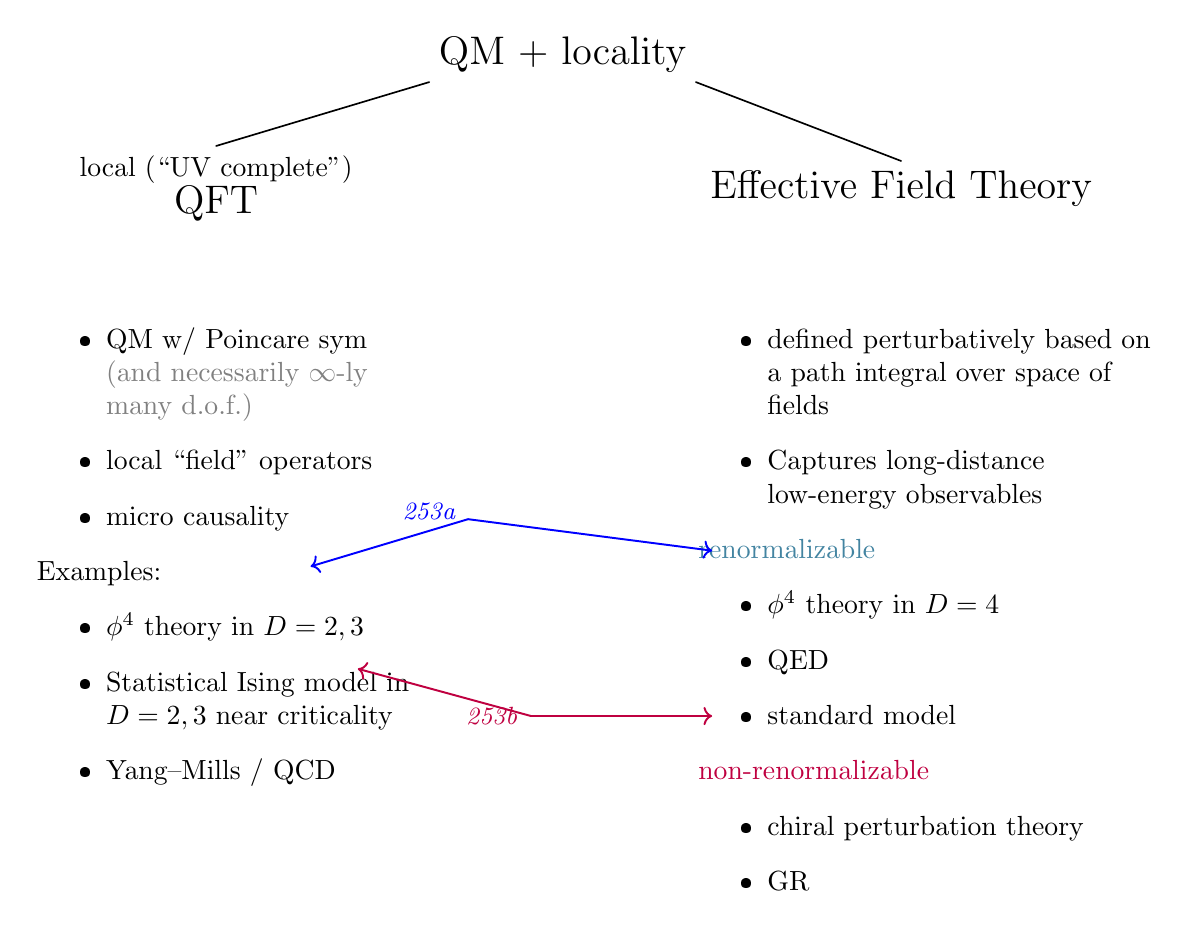
\begin{tikzpicture}[
  every node/.style={align=left},
  branch/.style={line width=0.6pt},
  note/.style={font=\small\itshape}
]
\node (root) at (0,0) {\Large QM + locality};
\node[align=center] (local) at (-4.4,-1.7) {local (``UV complete'')\\ \Large QFT};
\node[align=center] (eft) at (4.3,-1.7) {\Large Effective Field Theory};
\draw[branch] (root.south west) -- (local.north);
\draw[branch] (root.south east) -- (eft.north);

\node[text width=5.0cm,anchor=north west] at (-6.8,-2.9) {
\begin{itemize}
  \item QM w/ Poincare sym\\
  {\color{gray}(and necessarily $\infty$-ly many d.o.f.)}
  \item local ``field'' operators
  \item micro causality
\end{itemize}
Examples:
\begin{itemize}
  \item $\phi^4$ theory in $D=2,3$
  \item Statistical Ising model in $D=2,3$ near criticality
  \item Yang--Mills / QCD
\end{itemize}
};

\node[text width=5.8cm,anchor=north west] at (1.6,-2.9) {
\begin{itemize}
  \item defined perturbatively based on a path integral over space of fields
  \item Captures long-distance low-energy observables
\end{itemize}
\textcolor{cyan!60!black}{renormalizable}
\begin{itemize}
  \item $\phi^4$ theory in $D=4$
  \item QED
  \item standard model
\end{itemize}
\textcolor{purple}{non-renormalizable}
\begin{itemize}
  \item chiral perturbation theory
  \item GR
\end{itemize}
};

\node[note,blue] at (-1.7,-5.8) {253a};
\draw[->,blue,line width=0.7pt] (-1.2,-5.9) -- (-3.2,-6.5);
\draw[->,blue,line width=0.7pt] (-1.2,-5.9) -- (1.9,-6.3);
\node[note,purple] at (-0.9,-8.4) {253b};
\draw[->,purple,line width=0.7pt] (-0.4,-8.4) -- (-2.6,-7.8);
\draw[->,purple,line width=0.7pt] (-0.4,-8.4) -- (1.9,-8.4);
\end{tikzpicture}
\end{center}

\section{Plan of the Course}

\begin{enumerate}
\item Lagrangian formulation of QM
\begin{itemize}
  \item path integral, regularization
  \item perturbation theory, Feynman diagrams
  \item renormalization and counter terms
\end{itemize}

\item Relativistic particles and fields
\begin{itemize}
  \item $\phi^4$ theory
  \item Green functions
  \item asymptotic states
  \item S-matrix, LSZ reduction
\end{itemize}

\item Particles and fields with spin
\begin{itemize}
  \item classification of relativistic particles
  \item fermions and gauge bosons
  \item QED
  \item Applications: electron $g$-factor, Lamb shift.
\end{itemize}
\end{enumerate}

\section{Relativistic Particles}

Prelude: why do we need ``field theory'' to describe QM of particles with
relativistic symmetry?

\begin{itemize}
  \item Hilbert space $\mathcal H$
  \begin{itemize}
    \item vacuum $\ket{\Omega}$,
    \[
      H\ket{\Omega}=0.
    \]
    \item single particle $\ket{\vec p}$,
    \[
      p^\mu=(p^0,\vec p)
      \qquad
      \text{$D$-dimensional}
    \]
    \[
      H\ket{\vec p}=\sqrt{\vec p^{\,2}+m^2}\ket{\vec p}.
    \]
    \item multi-particle
    \[
      \ket{\vec p_1,\ldots,\vec p_n}
      \qquad
      \text{(non-interacting)}
    \]
    \[
      H=\sum_i \sqrt{\vec p_i^{\,2}+m^2}.
    \]
  \end{itemize}
\end{itemize}

Equivalently, we can introduce creation and annihilation operators:
\[
  \ket{\vec p}=a^\dagger_{\vec p}\ket{\Omega}.
\]

\[
  \ket{\vec p_1,\vec p_2}
  =
  a^\dagger_{\vec p_1}a^\dagger_{\vec p_2}\ket{\Omega},
  \qquad \text{etc.}
\]

\[
  [a,a]=[a^\dagger,a^\dagger]=0,
  \qquad
  [a_{\vec p},a^\dagger_{\vec p'}]
  =
  \delta^{(D-1)}(\vec p-\vec p'),
\]
so that
\[
  \braket{\vec p}{\vec p'}
  =
  \delta^{(D-1)}(\vec p-\vec p').
\]

We can then express the Hamiltonian as
\[
  H
  =
  \int \dd^{D-1}\vec p\,
  \sqrt{\vec p^{\,2}+m^2}\,
  a^\dagger_{\vec p}a_{\vec p}.
\]

This is a QM system of free relativistic particles.

What about interacting particles?
\[
  H=H_0+H_{\mathrm{int}},
\]
with possible terms such as
\[
  a^\dagger a^\dagger a,\qquad
  a a a^\dagger,\qquad \ldots
\]

It is not easy to find $H_{\mathrm{int}}$ that respects relativistic symmetry!

\section{Causality and Local Field Operators}

Issue: causality.

\begin{center}
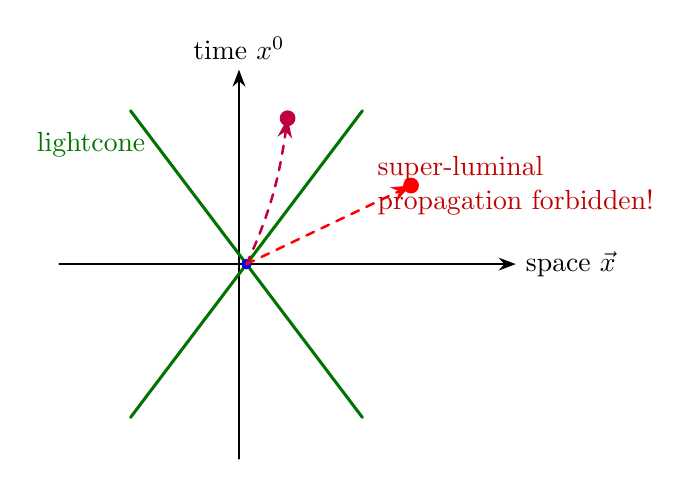
\begin{tikzpicture}[scale=0.95,>=Stealth]
\draw[->,line width=0.7pt] (-0.1,-2.6) -- (-0.1,2.6)
  node[above] {time $x^0$};
\draw[->,line width=0.7pt] (-2.5,0) -- (3.6,0)
  node[right] {space $\vec x$};
\draw[green!45!black,line width=1.1pt] (0,0) -- (-1.55,2.05)
  node[pos=0.78,left] {lightcone};
\draw[green!45!black,line width=1.1pt] (0,0) -- (1.55,2.05);
\draw[green!45!black,line width=1.1pt] (0,0) -- (-1.55,-2.05);
\draw[green!45!black,line width=1.1pt] (0,0) -- (1.55,-2.05);
\fill[blue] (0,0) circle (2pt);
\draw[purple,dashed,line width=0.9pt,->] (0,0) .. controls (0.35,0.75) and (0.45,1.25) .. (0.55,1.95);
\fill[purple] (0.55,1.95) circle (3pt);
\draw[red,dashed,line width=0.9pt,->] (0,0) -- (2.2,1.05);
\fill[red] (2.2,1.05) circle (3pt);
\node[red!75!black,align=left] at (3.6,1.05)
  {super-luminal\\ propagation forbidden!};
\end{tikzpicture}
\end{center}

In a generic QM system, signal propagation can be instantaneous.

In a relativistic system, expect local disturbance to be represented by
``field operator''
\[
  \hat\phi(x),
  \qquad
  x^\mu=(x^0,\vec x).
\]
The $x^\mu$ are merely parameters, not themselves operators.

\[
  \hat\phi(x)\ \text{and}\ \hat\phi(x')
\]
are related by Poincare symmetry.

\subsection{Poincare covariance}

\[
  x^\mu \longmapsto x'^\mu
  =
  \Lambda^\mu{}_\nu x^\nu+a^\mu,
\]
where
\[
  \eta_{\alpha\beta}\Lambda^\alpha{}_\mu\Lambda^\beta{}_\nu
  =
  \eta_{\mu\nu},
  \qquad
  \eta_{\mu\nu}=(-1,1,\ldots,1).
\]

In QM, represented by a unitary operator $U(\Lambda,a)$, such that
\[
  \hat\phi(\Lambda x+a)
  =
  U(\Lambda,a)\hat\phi(x)\bigl(U(\Lambda,a)\bigr)^{-1}.
\]

It suffices to study the infinitesimal version
\[
  \Lambda^\mu{}_\nu=\delta^\mu{}_\nu+\omega^\mu{}_\nu,
  \qquad
  a^\mu=\epsilon^\mu,
\]
small, keeping only first order,
\[
  U(\Lambda,a)
  =
  1-\ii\epsilon^\mu P_\mu+\frac{\ii}{2}\omega_{\mu\nu}J^{\mu\nu}.
\]
Here $P_\mu$ is energy-momentum, and $J^{\mu\nu}$ contains boosts and angular
momentum.

\[
  U(\Lambda',a')U(\Lambda,a)
  =
  U(\Lambda'\Lambda,\Lambda'a+a').
\]

\[
  [P^\mu,P^\nu]=0,
\]
\[
  [P^\mu,J^{\rho\sigma}]
  =
  -\ii\left(\eta^{\mu\rho}P^\sigma-\eta^{\mu\sigma}P^\rho\right),
\]
\[
  [J^{\mu\nu},J^{\rho\sigma}]
  =
  -\ii\left(
    \eta^{\mu\rho}J^{\nu\sigma}
    -\eta^{\nu\rho}J^{\mu\sigma}
    -(\rho\leftrightarrow\sigma)
  \right).
\]

\subsection{Microcausality}

Microcausality:
\[
  [\hat\phi(x),\hat\phi(y)]=0
\]
whenever $x,y$ are spacelike-separated, i.e.
\[
  (x-y)^2
  \equiv
  -(x^0-y^0)^2+(\vec x-\vec y)^2
  >0.
\]

What about our model of free relativistic particles?
\[
  H=\int \dd^{D-1}\vec p\,\sqrt{\vec p^{\,2}+m^2}\,
  a^\dagger_{\vec p}a_{\vec p},
\]
\[
  \vec P=\int \dd^{D-1}\vec p\,\vec p\,
  a^\dagger_{\vec p}a_{\vec p},
  \qquad
  P^\mu=(H,\vec P).
\]

Does $\hat\phi(x)$ exist? Yes!
\[
  \hat\phi(x)
  =
  \int
  \frac{\dd^{D-1}\vec p}
       {\sqrt{(2\pi)^{D-1}2\omega_{\vec p}}}
  \left(
    a_{\vec p}\ee^{\ii p\cdot x}
    +
    a^\dagger_{\vec p}\ee^{-\ii p\cdot x}
  \right).
\]

\[
  p\cdot x \equiv \vec p\cdot \vec x-\omega_{\vec p}x^0,
  \qquad
  \omega_{\vec p}\equiv\sqrt{\vec p^{\,2}+m^2}.
\]

Check microcausality:
\[
\begin{aligned}
[\hat\phi(x),\hat\phi(y)]
&=
\int
\frac{\dd^{D-1}\vec p}{(2\pi)^{D-1}2\omega_{\vec p}}
\left[
  \ee^{\ii p\cdot(x-y)}
  -
  \ee^{-\ii p\cdot(x-y)}
\right]
\\
&=
\int
\frac{\dd^D p}{(2\pi)^{D-1}}\,
\theta(p^0)\delta(p^2+m^2)
\left[
  \ee^{\ii p\cdot(x-y)}
  -
  \ee^{-\ii p\cdot(x-y)}
\right].
\end{aligned}
\]

The measure and mass-shell factor are invariant under
\[
  p^\mu\longmapsto \Lambda^\mu{}_\nu p^\nu,
\]
and the result is a function of $(x-y)^2$ only.

If $(x-y)^2>0$, WLOG can take
\[
  x^0-y^0=0,
  \qquad
  \vec x-\vec y\neq 0.
\]
The integrand is odd under $\vec p\mapsto-\vec p$, thus
\[
  \int \cdots =0,
\]
i.e.
\[
  [\hat\phi(x),\hat\phi(y)]=0
  \qquad
  \text{for }(x-y)^2>0.
\]

\subsection{Interacting theories}

Can also verify that
\[
  U(\Lambda,a)\hat\phi(x)\bigl(U(\Lambda,a)\bigr)^{-1}
  =
  \hat\phi(\Lambda x+a).
\]

Postulate that the properties
\begin{itemize}
  \item Hilbert space $\mathcal H$,
  \item Poincare sym $U(\Lambda,a)$,
  \item Poincare-invariant vacuum $\ket{\Omega}$,
  \item local ``field'' operators $\hat\phi(x)$ that obey Poincare covariance and
  microcausality,
\end{itemize}
hold for systems of interacting relativistic particles as well!

How to construct such theories?

It is useful to work with a formalism in which Poincare sym is manifest.

\section{Lagrangian Formalism}

Recall in classical mechanics:

\begin{center}
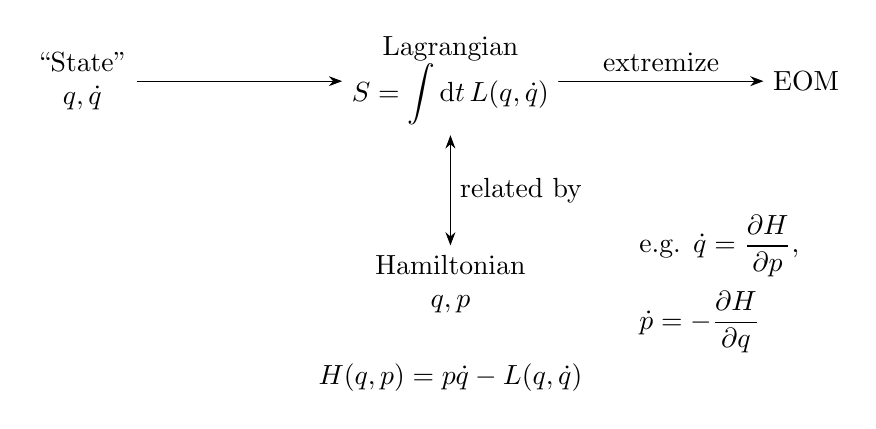
\begin{tikzpicture}[>=Stealth,node distance=2.6cm]
\node[align=center] (state) {``State''\\ $q,\dot q$};
\node[align=center,right=of state] (lag) {Lagrangian\\ $S=\displaystyle\int \dd t\,L(q,\dot q)$};
\node[align=center,right=of lag] (eom) {EOM};
\node[align=center,below=1.4cm of lag] (ham) {Hamiltonian\\ $q,p$};
\draw[->] (state) -- (lag);
\draw[->] (lag) -- node[above]{extremize} (eom);
\draw[<->] (lag) -- node[right] {related by} (ham);
\node[align=left,right=1.2cm of ham] {
e.g. $\dot q=\dfrac{\partial H}{\partial p}$,\\[0.4em]
$\dot p=-\dfrac{\partial H}{\partial q}$};
\node[align=center,below=0.4cm of ham] {
$H(q,p)=p\dot q-L(q,\dot q)$};
\end{tikzpicture}
\end{center}

QM:

\begin{center}
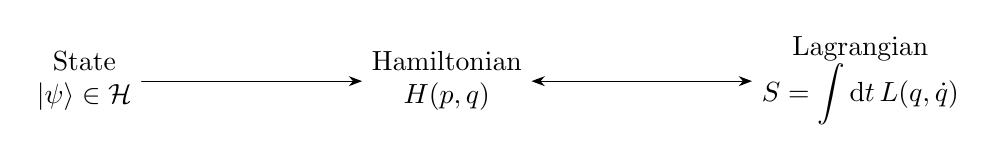
\begin{tikzpicture}[>=Stealth,node distance=2.8cm]
\node[align=center] (state) {State\\ $\ket{\psi}\in\mathcal H$};
\node[align=center,right=of state] (ham) {Hamiltonian\\ $H(p,q)$};
\node[align=center,right=of ham] (lag) {Lagrangian\\ $S=\displaystyle\int \dd t\,L(q,\dot q)$};
\draw[->] (state) -- (ham);
\draw[<->] (ham) -- (lag);
\end{tikzpicture}
\end{center}

\subsection{Time Evolution and the Path Integral Measure}

Schrodinger:
\[
  \ket{\psi}\longmapsto U(t)\ket{\psi},
  \qquad
  U(t)=\ee^{-\frac{\ii}{\hbar}\hat Ht}.
\]

Heisenberg:
\[
  \hat O\longmapsto \bigl(U(t)\bigr)^{-1}\hat O\,U(t)
  \equiv
  \hat O(t),
  \qquad
  \dot{\hat O}(t)=\frac{\ii}{\hbar}\,[\hat H,\hat O(t)].
\]

The Lagrangian transition amplitude is written
\[
  \bra{q_f}U(T)\ket{q_i}
  =
  \int
  \left[\mathcal D q\right]_{\substack{q(T)=q_f\\ q(0)=q_i}}
  \ee^{\frac{\ii}{\hbar}S}.
\]
The subtle object here is the path-integral measure $[\mathcal Dq]$.

To revisit its derivation, consider time evolution by $T$ in $N$ steps:
\begin{center}
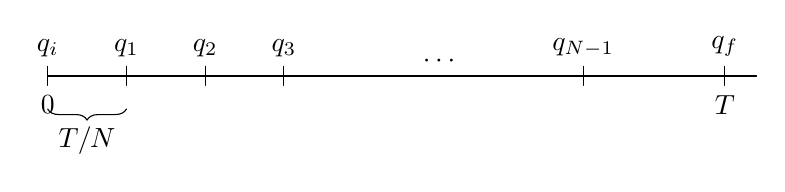
\begin{tikzpicture}[>=Stealth]
\draw[line width=0.6pt] (0,0) -- (9,0);
\foreach \x/\lab in {
  0/{q_i},
  1/{q_1},
  2/{q_2},
  3/{q_3},
  6.8/{q_{N-1}},
  8.6/{q_f}
}{
  \draw (\x,0.12) -- (\x,-0.12);
  \node[above] at (\x,0.12) {$\lab$};
}
\node[below] at (0,-0.12) {$0$};
\draw[decorate,decoration={brace,amplitude=4pt,mirror}]
  (0,-0.42) -- node[below=3pt] {$T/N$} (1,-0.42);
\node[below] at (8.6,-0.12) {$T$};
\node at (5,0.18) {$\cdots$};
\end{tikzpicture}
\end{center}

\[
\begin{aligned}
  \bra{q_f}U(T)\ket{q_i}
  &=
  \int \dd q_1\cdots \dd q_{N-1}\,
  \bra{q_f}\ee^{-\frac{\ii}{\hbar}\hat H\frac{T}{N}}\ket{q_{N-1}}
  \cdots
  \bra{q_1}\ee^{-\frac{\ii}{\hbar}\hat H\frac{T}{N}}\ket{q_i}
  \\
  &=
  \int \dd q_1\cdots \dd q_{N-1}\,
  \prod_{n=0}^{N-1}
  \bra{q_{n+1}}\ee^{-\frac{\ii}{\hbar}\hat H\frac{T}{N}}\ket{q_n},
  \qquad
  q_f\equiv q_N,\quad q_i\equiv q_0.
\end{aligned}
\]

Insert a complete set of momentum eigenstates:
\[
\begin{aligned}
  \bra{q_f}U(T)\ket{q_i}
  &=
  \int
  \prod_{n=1}^{N-1}\dd q_n
  \prod_{n=0}^{N-1}\frac{\dd^D p_n}{(2\pi\hbar)^D}\,
  \bra{q_{n+1}}p_n\rangle
  \bra{p_n}\ee^{-\frac{\ii}{\hbar}\hat H\frac{T}{N}}\ket{q_n}
  \\
  &=
  \int
  \prod_{n=1}^{N-1}\dd q_n
  \prod_{n=0}^{N-1}\frac{\dd^D p_n}{(2\pi\hbar)^D}
  \exp\left\{
    \frac{\ii}{\hbar}
    \sum_{n=0}^{N-1}
    \left[
      p_n\cdot(q_{n+1}-q_n)
      -H(q_n,p_n)\frac{T}{N}
      +O\!\left(\hbar,\left(\frac{T}{N}\right)^2\right)
    \right]
  \right\}.
\end{aligned}
\]
Here $H(q,p)$ denotes the classical Hamiltonian.

Formally, in the $N\to\infty$ limit,
\[
  \bra{q_f}U(T)\ket{q_i}
  =
  \int \mathcal Dq\,\mathcal Dp\,
  \exp\left\{
    \frac{\ii}{\hbar}
    \int_0^T \dd t\,
    \bigl(p\cdot\dot q-H(q,p)\bigr)
  \right\}.
\]
The measure is defined via regularization, for example by discretizing time.
The action contains $O(\hbar)$ ambiguities, or counterterms; these ambiguities
are tied to the scheme of regularization.

For example, one may replace
\[
  \int_0^T \dd t\,p\,\dot q
\]
by either
\[
  \sum_{n=0}^{N-1}p_n(q_{n+1}-q_n)
  \qquad\text{or}\qquad
  \sum_{n=0}^{N-1}p_{n+1}(q_{n+1}-q_n).
\]
The exact representation of the time evolution is schematically
\[
  \cdots
  \bra{q_{n+1}}p_n\rangle
  \bra{p_n}\ee^{-\frac{\ii}{\hbar}\hat H\frac{T}{N}}\ket{q_n}
  \cdots
\]
in the former case, with
\[
  \bra{p_n}\hat H\ket{q_n}
  =
  H(p_n,q_n)\bra{p_n}q_n\rangle,
\]
and
\[
  \cdots
  \bra{p_{n+1}}q_{n+1}\rangle
  \bra{q_{n+1}}\ee^{-\frac{\ii}{\hbar}\hat H\frac{T}{N}}\ket{p_n}
  \cdots
\]
in the latter case, with
\[
  \bra{q_n}\hat H\ket{p_n}
  =
  H'(p_n,q_n)\bra{q_n}p_n\rangle.
\]
The functions $H(p_n,q_n)$ and $H'(p_n,q_n)$ can differ at order $O(\hbar)$.

If $H(q,p)$ is quadratic in $p$, for example
\[
  H(q,p)=\frac{p^2}{2m}+V(q),
\]
then $p(t)$ can be integrated out as a Gaussian, leaving
\[
  \int [\mathcal Dq]\,
  \ee^{\frac{\ii}{\hbar}\int_0^T \dd t\,L(q,\dot q)}.
\]
For this example
\[
  L(q,\dot q)=\frac12 m\dot q^2-V(q),
\]
and the Gaussian determinant of $p(t)$ is absorbed into the measure.

More generally, a Lagrangian in generalized coordinates typically takes the
form
\[
  L=\frac12 G_{\alpha\beta}(q)\dot q^\alpha\dot q^\beta-V(q)
  \qquad
  \text{(e.g. rotating 3D rigid body),}
\]
so that
\[
  H=\frac12\bigl(G^{-1}(q)\bigr)^{\alpha\beta}p_\alpha p_\beta+V(q)+O(\hbar).
\]
The phase-space path integral
\[
  \int \mathcal Dp\,\mathcal Dq\,
  \ee^{\frac{\ii}{\hbar}\int \dd t\,(p_\alpha\dot q^\alpha-H(p,q))}
\]
becomes
\[
  \int [\mathcal Dq]\,
  \ee^{\frac{\ii}{\hbar}\int \dd t\,L(q,\dot q)},
\]
with the regularized measure of the form
\[
  [\mathcal Dq]
  \sim
  \prod_n
  \frac{\dd q_n^\alpha}{\sqrt{2\pi\ii\hbar\,T/N}}\,
  \sqrt{\det G_{\alpha\beta}(q_n)}.
\]

\subsection{Correlation Functions and Wick Rotation}

Consider a correlation function in the ground state $\ket{0}$, for example
\[
  G(t)=\bra{0}\hat q(t)\hat q(0)\ket{0}.
\]
Insert a basis of $\hat H$-eigenstates, $\hat H\ket{n}=E_n\ket{n}$:
\[
\begin{aligned}
  G(t)
  &=
  \sum_n
  \bra{0}\hat q(t)\ket{n}\bra{n}\hat q(0)\ket{0}
  \\
  &=
  \sum_n
  \bra{0}
  \ee^{\frac{\ii}{\hbar}\hat Ht}
  \hat q(0)
  \ee^{-\frac{\ii}{\hbar}\hat Ht}
  \ket{n}
  \bra{n}\hat q(0)\ket{0}
  \\
  &=
  \sum_n
  \bra{0}\hat q(0)\ket{n}
  \bra{n}\hat q(0)\ket{0}\,
  \ee^{-\frac{\ii}{\hbar}(E_n-E_0)t}.
\end{aligned}
\]
Since $E_n-E_0\ge 0$, $G(t)$ can be analytically continued as a function of
complex $t$, provided $\operatorname{Im}t<0$, so that the sum converges
(Paley--Wiener theorem).

For example, set
\[
  t=-\ii\tau,
  \qquad
  \tau\in\mathbb R_+,
\]
the Wick rotation. Then
\[
  \bra{0}\hat q(t)\hat q(0)\ket{0}
  =
  \sum_n
  \bra{0}\hat q(0)\ket{n}
  \bra{n}\hat q(0)\ket{0}\,
  \ee^{-\frac{1}{\hbar}(E_n-E_0)\tau}.
\]

Assuming a gap $E_1-E_0>0$, one can replace $\ket{0}$ by
\[
  \lim_{T\to\infty}
  \ee^{-\frac{1}{\hbar}(\hat H-E_0)T}\ket{\psi},
\]
up to overall normalization, for any generic state $\ket{\psi}$ with nonzero
overlap with $\ket{0}$. Thus
\[
  \bra{0}\hat q(t)\hat q(0)\ket{0}
  =
  \lim_{T\to\infty}
  \frac{
  \bra{\psi}
  \ee^{-\frac{1}{\hbar}\hat H T}
  \hat q(t)\hat q(0)
  \ee^{-\frac{1}{\hbar}\hat H T}
  \ket{\psi}
  }{
  \bra{\psi}\ee^{-\frac{2}{\hbar}\hat H T}\ket{\psi}
  }.
\]

\begin{center}
\begin{tikzpicture}[>=Stealth,scale=0.95]
\draw[->] (-3.2,0) -- (3.4,0) node[right] {$\operatorname{Re}t$};
\draw[->] (0,-2.0) -- (0,2.3) node[above] {$-\operatorname{Im}t$};
\draw[green!45!black,line width=1.1pt,->] (0,0) -- (2.1,0);
\draw[blue,line width=1.1pt,->] (0,-1.6) -- (0,-0.15);
\draw[purple,line width=1.1pt,->] (0,0.05) -- (0,1.7);
\fill[orange] (0,0) circle (2pt);
\fill[red] (2.1,0) circle (2pt);
\end{tikzpicture}
\end{center}

Alternatively,
\[
  G(t=-\ii\tau)
  =
  \bra{0}
  \ee^{\frac{1}{\hbar}\hat H\tau}
  \hat q(0)
  \ee^{-\frac{1}{\hbar}\hat H\tau}
  \hat q(0)
  \ket{0},
\]
and
\[
  G(t=-\ii\tau)
  =
  \lim_{T\to\infty}
  \frac{
  \bra{\psi}
  \ee^{-\frac{1}{\hbar}\hat H(T-\tau)}
  \hat q(0)
  \ee^{-\frac{1}{\hbar}\hat H\tau}
  \hat q(0)
  \ee^{-\frac{1}{\hbar}\hat H T}
  \ket{\psi}
  }{
  \bra{\psi}\ee^{-\frac{2}{\hbar}\hat H T}\ket{\psi}
  }.
\]

\begin{center}
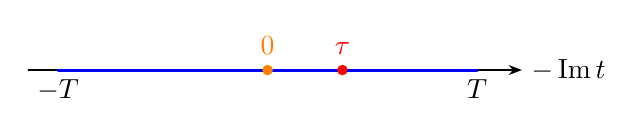
\begin{tikzpicture}[>=Stealth,scale=0.95]
\draw[->] (-3.2,0) -- (3.4,0) node[right] {$-\operatorname{Im}t$};
\draw[blue,line width=1.1pt] (-2.8,0) -- (2.8,0);
\fill[orange] (0,0) circle (2pt) node[above=2pt] {$0$};
\fill[red] (1.0,0) circle (2pt) node[above=2pt] {$\tau$};
\node[below] at (-2.8,0) {$-T$};
\node[below] at (2.8,0) {$T$};
\end{tikzpicture}
\end{center}

From the path integral,
\[
  \bra{0}\hat q(t)\hat q(0)\ket{0}
  =
  \lim_{\substack{\operatorname{Im}t_f\to-\infty\\
                  \operatorname{Im}t_i\to+\infty}}
  \frac{
  \int [\mathcal Dq]\,
  \ee^{\frac{\ii}{\hbar}\int_{t_i}^{t_f}L[q,\dot q]\dd t}\,
  q(t)q(0)
  }{
  \int [\mathcal Dq]\,
  \ee^{\frac{\ii}{\hbar}\int_{t_i}^{t_f}L[q,\dot q]\dd t}
  }.
\]

Under Wick rotation, $t=-\ii\tau$, still using the same notation,
\[
  \dd t\,\dot q=+\ii\,\dd\tau\,q',
  \qquad
  q'=\frac{\dd q}{\dd\tau}.
\]
Define
\[
  L^E[q,q']\equiv -L[q,\ii q']
\]
so that
\[
  \ee^{\frac{\ii}{\hbar}\int L[q,\dot q]\dd t}
  =
  \ee^{-\frac{1}{\hbar}\int L^E[q,q']\dd\tau}.
\]
For example, if
\[
  L[q,\dot q]=\frac12\dot q^2-V(q),
\]
then
\[
  L^E[q,q']=\frac12(q')^2+V(q).
\]

How do we evaluate the path integral? The key is to find a convenient
regularized expression of the measure $[\mathcal Dq]$. For instance, write
\[
  q(\tau)=\sum_n q_n f_n(\tau),
\]
where $f_n$ is a suitable basis of functions, and ask whether
\[
  [\mathcal Dq]\stackrel{?}{=}\prod_n\dd q_n.
\]

\subsection{Harmonic Oscillator Example}

Consider
\[
  H=\frac{p^2+\omega^2q^2}{2}
  \qquad\Longleftrightarrow\qquad
  L=\frac12\dot q^2-\frac12\omega^2q^2.
\]
After the Wick rotation $t=-\ii\tau$, evaluate
\[
  \int[\mathcal Dq]\,\ee^{-\frac{1}{\hbar}S^E}\cdots.
\]
Choose boundary conditions in imaginary time, for example
\[
  q(-T)=q(T)=0.
\]

\begin{center}
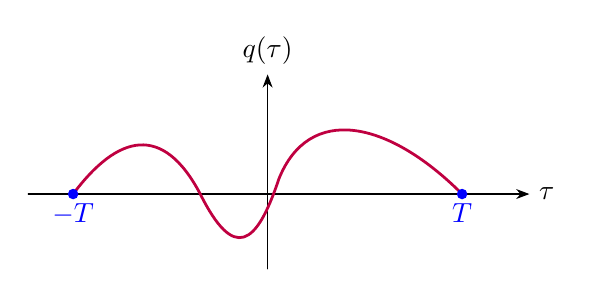
\begin{tikzpicture}[>=Stealth,scale=0.95]
\draw[->] (-3.2,0) -- (3.5,0) node[right] {$\tau$};
\draw[->] (0,-1.0) -- (0,1.6) node[above] {$q(\tau)$};
\draw[purple,line width=1pt]
  (-2.6,0)
  .. controls (-2.0,0.8) and (-1.4,0.95) .. (-0.9,0.0)
  .. controls (-0.45,-0.9) and (-0.15,-0.7) .. (0.15,0.2)
  .. controls (0.55,1.2) and (1.6,1.0) .. (2.6,0);
\fill[blue] (-2.6,0) circle (2pt) node[below] {$-T$};
\fill[blue] (2.6,0) circle (2pt) node[below] {$T$};
\end{tikzpicture}
\end{center}

Expand $q(\tau)$ on a Fourier basis:
\[
  q(\tau)=\sum_{n=1}^\infty q_n f_n(\tau),
  \qquad
  f_n(\tau)=\frac{1}{\sqrt{T}}\,
  \sin\frac{n\pi(\tau+T)}{2T}.
\]
The functions $f_n(\tau)$ obey the prescribed boundary condition and are
orthonormal with respect to a suitable inner product:
\[
  (f_n,f_m)
  :=
  \int_{-T}^{T}f_n^*(\tau)f_m(\tau)\dd\tau
  =
  \delta_{nm}.
\]
For convenience, they also diagonalize the kinetic term in the action:
\[
\begin{aligned}
  S^E
  &=
  \int_{-T}^{T}
  \left[
    \frac12(q')^2+\frac12\omega^2q^2
  \right]\dd\tau
  \\
  &=
  \sum_{n=1}^{\infty}
  \left[
    \frac12\left(\frac{n\pi}{2T}\right)^2
    +
    \frac12\omega^2
  \right]q_n^2.
\end{aligned}
\]
Therefore
\[
  \int[\mathcal Dq]\,\ee^{-\frac{1}{\hbar}S^E}\cdots
  \sim
  \int \prod_{n=1}^{\infty}\dd q_n\,
  \exp\left\{
    -\frac{1}{\hbar}
    \sum_{n=1}^{\infty}
    \frac12
    \left[
      \left(\frac{n\pi}{2T}\right)^2+\omega^2
    \right]q_n^2
  \right\}
  \cdots,
\]
a Gaussian.

Write the normalized expectation value as
\[
  \langle \cdots\rangle
  =
  \frac{\int[\mathcal Dq]\,\ee^{-\frac{1}{\hbar}S^E}\cdots}
       {\int[\mathcal Dq]\,\ee^{-\frac{1}{\hbar}S^E}}.
\]
It is easy to evaluate using the Gaussian integral:
\[
  \langle q_n q_m\rangle
  =
  \delta_{nm}
  \frac{\hbar}{\left(\frac{n\pi}{2T}\right)^2+\omega^2}.
\]
Therefore
\[
\begin{aligned}
  \langle q(\tau_1)q(\tau_2)\rangle
  &=
  \sum_{n,m=1}^{\infty}
  \langle q_nq_m\rangle f_n(\tau_1)f_m(\tau_2)
  \\
  &=
  \sum_{n=1}^{\infty}
  \frac{\hbar}{\left(\frac{n\pi}{2T}\right)^2+\omega^2}
  \frac{1}{T}
  \sin\frac{n\pi(\tau_1+T)}{2T}\,
  \sin\frac{n\pi(\tau_2+T)}{2T}.
\end{aligned}
\]
Take the limit $T\to\infty$. With
\[
  \frac{n\pi}{2T}\equiv k,
  \qquad
  \sum_n\frac{\pi}{2T}\cdots\longrightarrow\int\dd k\,\cdots,
\]
we get
\[
  \langle q(\tau_1)q(\tau_2)\rangle
  =
  \frac{2\hbar}{\pi}
  \int_0^\infty\dd k\,
  \frac{
    \sin k(\tau_1+T)\,\sin k(\tau_2+T)
  }{k^2+\omega^2}.
\]
Equivalently,
\[
\begin{aligned}
  \langle q(\tau_1)q(\tau_2)\rangle
  &=
  \frac{\hbar}{\pi}
  \int_{-\infty}^{\infty}
  \frac{\dd k}{k^2+\omega^2}
  \biggl[
    \frac14\ee^{\ii k(\tau_1-\tau_2)}
    +\frac14\ee^{-\ii k(\tau_1-\tau_2)}
    \\
    &\hspace{4.1cm}
    -\frac14\ee^{\ii k(\tau_1+\tau_2+2T)}
    -\frac14\ee^{-\ii k(\tau_1+\tau_2+2T)}
  \biggr].
\end{aligned}
\]

Consider
\[
  \int_{-\infty}^{\infty}
  \dd k\,\frac{\ee^{\ii k\tau}}{k^2+\omega^2}.
\]
The integrand, as an analytic function in the complex $k$-plane, has poles at
$k=\pm\ii\omega$.

\begin{center}
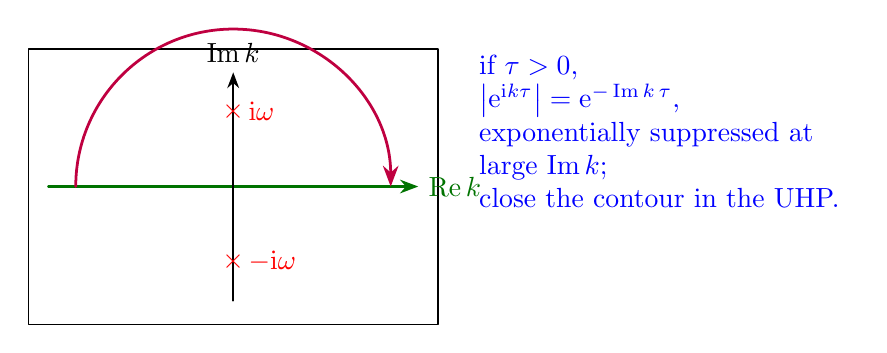
\begin{tikzpicture}[>=Stealth,scale=1.0]
\draw[line width=0.6pt] (-2.6,-1.75) rectangle (2.6,1.75);
\draw[->,green!45!black,line width=0.8pt] (-2.35,0) -- (2.35,0)
  node[right] {$\operatorname{Re}k$};
\draw[->,line width=0.6pt] (0,-1.45) -- (0,1.45)
  node[above] {$\operatorname{Im}k$};
\draw[purple,line width=1.0pt,->]
  (-2.0,0) arc[start angle=180,end angle=0,radius=2.0];
\node[red] at (0,0.95) {$\times$};
\node[red,right=2pt] at (0,0.95) {$\ii\omega$};
\node[red] at (0,-0.95) {$\times$};
\node[red,right=2pt] at (0,-0.95) {$-\ii\omega$};
\node[blue,align=left,text width=4.7cm,anchor=west] at (3.0,0.7)
  {if $\tau>0$,\\
   $\left|\ee^{\ii k\tau}\right|=\ee^{-\operatorname{Im}k\,\tau}$,\\
   exponentially suppressed at large $\operatorname{Im}k$;\\
   close the contour in the UHP.};
\end{tikzpicture}
\end{center}

For $\tau>0$,
\[
\begin{aligned}
  \int_{-\infty}^{\infty}
  \dd k\,\frac{\ee^{\ii k\tau}}{k^2+\omega^2}
  &=
  2\pi\ii\,
  \operatorname*{Res}_{k=\ii\omega}
  \frac{\ee^{\ii k\tau}}{k^2+\omega^2}
  \\
  &=
  \frac{\pi}{\omega}\ee^{-\omega\tau}.
\end{aligned}
\]
Similarly, for $\tau<0$, the result is
\[
  \frac{\pi}{\omega}\ee^{\omega\tau}.
\]
Returning to the two-point function, the terms involving
$\tau_1+\tau_2+2T$ vanish as $T\to\infty$, and
\[
  \langle q(\tau_1)q(\tau_2)\rangle
  =
  \frac{\hbar}{\omega}
  \left(
    \frac12\ee^{-\omega|\tau_1-\tau_2|}
    -
    \frac12\ee^{-\omega(\tau_1+\tau_2+2T)}
  \right)
  \longrightarrow
  \frac{\hbar}{2\omega}\ee^{-\omega|\tau_1-\tau_2|}.
\]

\subsection{Gaussian Integrals and Wick Contractions}

Consider a general Gaussian integral
\[
  Z[\vec J]
  =
  \int\dd^N\vec q\,
  \exp\left\{
    -\frac12\vec q^{\,T}A\vec q+\vec J\cdot\vec q
  \right\},
  \qquad
  A=A^T,
\]
where $A$ is a symmetric matrix. Then
\[
  Z[\vec J]
  =
  (2\pi)^{N/2}(\det A)^{-1/2}
  \exp\left\{\frac12\vec J^{\,T}A^{-1}\vec J\right\}.
\]
For any function $F(\vec q)$, define
\[
\begin{aligned}
  \langle F(\vec q)\rangle
  &:=
  \frac{1}{Z[0]}
  \int\dd^N\vec q\,
  \ee^{-\frac12\vec q^{\,T}A\vec q}F(\vec q)
  \\
  &=
  \left.
  \frac{1}{Z[0]}
  F\left(\frac{\partial}{\partial\vec J}\right)Z[\vec J]
  \right|_{\vec J=0}.
\end{aligned}
\]
For example,
\[
  \langle q_n\rangle=0,
\]
and
\[
\begin{aligned}
  \langle q_nq_m\rangle
  &=
  \left.
  \frac{\partial}{\partial J_n}\frac{\partial}{\partial J_m}
  \exp\left\{\frac12 J_p(A^{-1})_{pq}J_q\right\}
  \right|_{\vec J=0}
  \\
  &=
  (A^{-1})_{nm}.
\end{aligned}
\]
For four variables,
\[
\begin{aligned}
  \langle q_nq_mq_rq_s\rangle
  &=
  \left.
  \frac{\partial}{\partial J_n}
  \frac{\partial}{\partial J_m}
  \frac{\partial}{\partial J_r}
  \frac{\partial}{\partial J_s}
  \exp\left\{\frac12 J_p(A^{-1})_{pq}J_q\right\}
  \right|_{\vec J=0}
  \\
  &=
  \left.
  \frac{\partial}{\partial J_n}
  \frac{\partial}{\partial J_m}
  \frac{\partial}{\partial J_r}
  \frac{\partial}{\partial J_s}
  \frac12\left(\frac12 J_p(A^{-1})_{pq}J_q\right)^2
  \right|_{\vec J=0}.
\end{aligned}
\]
The derivatives pick all possible ways of connecting the four labels.

\begin{center}
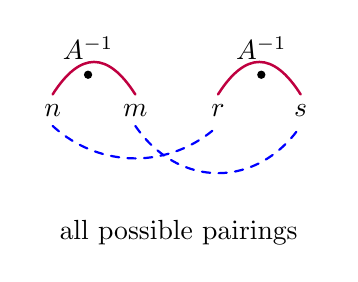
\begin{tikzpicture}[scale=1.0,baseline=(current bounding box.center)]
\node (n) at (0,0) {$n$};
\node (m) at (1.05,0) {$m$};
\node (r) at (2.1,0) {$r$};
\node (s) at (3.15,0) {$s$};
\fill (0.45,0.45) circle (1.5pt) node[above=2pt] {$A^{-1}$};
\fill (2.65,0.45) circle (1.5pt) node[above=2pt] {$A^{-1}$};
\draw[purple,line width=0.9pt] (n.north) .. controls (0.35,0.75) and (0.7,0.75) .. (m.north);
\draw[purple,line width=0.9pt] (r.north) .. controls (2.45,0.75) and (2.8,0.75) .. (s.north);
\draw[blue,dashed,line width=0.8pt] (n.south) .. controls (0.6,-0.75) and (1.5,-0.75) .. (r.south);
\draw[blue,dashed,line width=0.8pt] (m.south) .. controls (1.6,-1.0) and (2.6,-1.0) .. (s.south);
\node[text width=3.6cm,align=center] at (1.6,-1.55)
  {all possible pairings};
\end{tikzpicture}
\end{center}

There are $4!=24$ such terms before grouping, and the result is
\[
  \langle q_nq_mq_rq_s\rangle
  =
  (A^{-1})_{nm}(A^{-1})_{rs}
  +(A^{-1})_{nr}(A^{-1})_{ms}
  +(A^{-1})_{ns}(A^{-1})_{mr}.
\]
This is the Wick contraction rule:
\[
  \langle q_nq_mq_r\cdots\rangle
  =
  \sum_{\text{all inequivalent Wick contractions}}
  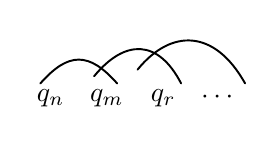
\begin{tikzpicture}[baseline=-0.55ex,scale=0.65]
    \node at (0,0) {$q_n$};
    \node at (1.1,0) {$q_m$};
    \node at (2.2,0) {$q_r$};
    \node at (3.3,0) {$\cdots$};
    \draw[line width=0.7pt] (-0.2,0.28) .. controls (0.35,0.9) and (0.75,0.9) .. (1.3,0.28);
    \draw[line width=0.7pt] (0.85,0.42) .. controls (1.45,1.15) and (2.1,1.15) .. (2.55,0.28);
    \draw[line width=0.7pt] (1.7,0.55) .. controls (2.35,1.35) and (3.2,1.35) .. (3.8,0.28);
  \end{tikzpicture},
\]
with
\[
  q_nq_m\ \hbox{contracted}\ :=\ (A^{-1})_{nm}.
\]

\subsection{Gaussian Functional Integrals}

Now generalize the Gaussian integral to a functional integral. In the following
formulas we set $\hbar=1$:
\[
  \vec q\longrightarrow q(\tau)
  \in
  \text{a linear space of real functions}
\]
with a suitable measure, and
\[
  \vec q\cdot\vec J
  \longrightarrow
  \int\dd\tau\,q(\tau)J(\tau).
\]
Consider the linear operator $A$,
\[
  A\cdot q(\tau):=\left(-\partial_\tau^2+\omega^2\right)q(\tau),
\]
and write its inverse as
\[
  A^{-1}\cdot g(\tau)
  =
  \int\dd\tau'\,G(\tau,\tau')g(\tau').
\]
The Green function obeys
\[
  \left(-\partial_\tau^2+\omega^2\right)G(\tau,\tau')
  =
  \delta(\tau-\tau').
\]
The Euclidean action is
\[
  S^E
  =
  \frac12(q,Aq)
  =
  \frac12\int\dd\tau\,q(\tau)\,A\cdot q(\tau),
\]
so
\[
  \langle q(\tau_1)q(\tau_2)\rangle
  =
  \frac{
    \int[\mathcal Dq]\,
    \ee^{-\frac12(q,Aq)}
    q(\tau_1)q(\tau_2)
  }{
    \int[\mathcal Dq]\,
    \ee^{-\frac12(q,Aq)}
  }.
\]

To avoid confusion with normalization in discretizing the integral in $\tau$,
we can obtain the answer using an integration-by-parts trick. Since
\[
  q(\tau_1)\ee^{-\frac12(q,Aq)}
  =
  -\left(A^{-1}\cdot\frac{\delta}{\delta q}\right)(\tau_1)
  \ee^{-\frac12(q,Aq)},
\]
we have
\[
\begin{aligned}
  &\int[\mathcal Dq]\,
  \ee^{-\frac12(q,Aq)}q(\tau_1)q(\tau_2)
  \\
  &\qquad =
  \int[\mathcal Dq]\,
  q(\tau_2)
  \left[
    -\left(A^{-1}\cdot\frac{\delta}{\delta q}\right)(\tau_1)
  \right]
  \ee^{-\frac12(q,Aq)}
  \\
  &\qquad =
  \int[\mathcal Dq]\,
  \ee^{-\frac12(q,Aq)}
  \left(A^{-1}\cdot\frac{\delta}{\delta q}\right)(\tau_1)
  q(\tau_2)
  \\
  &\qquad =
  \int[\mathcal Dq]\,
  \ee^{-\frac12(q,Aq)}
  \int\dd\tau'\,G(\tau_1,\tau')\delta(\tau'-\tau_2).
\end{aligned}
\]
Thus
\[
  \langle q(\tau_1)q(\tau_2)\rangle
  =
  G(\tau_1,\tau_2).
\]

Alternatively, work with the Fourier transformed variable
\[
  q(\tau)
  =
  \int_{-\infty}^{\infty}
  \frac{\dd k}{2\pi}\,\tilde q(k)\ee^{\ii k\tau},
  \qquad
  \tilde q^{\,*}(k)=\tilde q(-k).
\]
Then
\[
  A\cdot\tilde q(k)=(k^2+\omega^2)\tilde q(k),
  \qquad
  A^{-1}\cdot\tilde q(k)=\frac{1}{k^2+\omega^2}\tilde q(k).
\]
Therefore
\[
  G(\tau,\tau')
  =
  \int_{-\infty}^{\infty}
  \frac{\dd k}{2\pi}\,
  \frac{\ee^{\ii k(\tau-\tau')}}{k^2+\omega^2}
  =
  \frac{\ee^{-\omega|\tau-\tau'|}}{2\omega},
\]
in agreement with the earlier direct evaluation, having set $\hbar=1$.

Since $A$ is diagonal in the $\tilde q(k)$ basis,
\[
\begin{aligned}
  S^E
  &=
  \frac12(q,Aq)
  =
  \frac12\int_{-\infty}^{\infty}\dd\tau\,q(\tau)A\cdot q(\tau)
  \\
  &=
  \frac12
  \int_{-\infty}^{\infty}
  \frac{\dd k}{2\pi}\,
  \tilde q(-k)(k^2+\omega^2)\tilde q(k).
\end{aligned}
\]
Using the same integration-by-parts trick,
\[
  \langle \tilde q(k_1)\tilde q(k_2)\rangle
  =
  \frac{2\pi\delta(k_1+k_2)}{k_1^2+\omega^2}.
\]

\subsection{Anharmonic Oscillator}

Example 2 is the anharmonic oscillator,
\[
  H=\frac{p^2}{2}+\frac{q^2}{2}+\frac{g}{4!}q^4,
\]
or equivalently
\[
  L=\frac12\dot q^{\,2}-\frac{q^2}{2}-\frac{g}{4!}q^4.
\]
Study its spectrum using
\[
  \bra{0}\hat q(\tau)\hat q(0)\ket{0},
  \qquad
  \tau>0.
\]
By inserting a complete set of energy eigenstates,
\[
  \bra{0}\hat q(\tau)\hat q(0)\ket{0}
  =
  \sum_n
  \left|\bra{n}\hat q(0)\ket{0}\right|^2
  \ee^{-E_n\tau}.
\]
The same correlation function is represented by the Euclidean path integral
\[
  \bra{0}\hat q(\tau)\hat q(0)\ket{0}
  =
  \frac{1}{Z}
  \int[\mathcal Dq]\,
  \ee^{-\int\dd\tau\,L^E}
  q(\tau)q(0),
\]
where
\[
  Z=\int[\mathcal Dq]\,\ee^{-\int\dd\tau\,L^E},
  \qquad
  L^E=\frac12(\partial_\tau q)^2+\frac{q^2}{2}+\frac{g}{4!}q^4.
\]
Expand in powers of $g$:
\[
  Z
  =
  \int[\mathcal Dq]\,
  \ee^{-\int\dd\tau\left(\frac12(\partial_\tau q)^2+\frac12q^2\right)}
  \sum_{n=0}^{\infty}
  \frac{1}{n!}
  \left(
    -\frac{g}{4!}\int\dd\tau'\,q^4(\tau')
  \right)^n.
\]
At this stage one assumes that exchanging the order of the functional integral
and the expansion in $g$ is allowed; this point will be revisited later.

Let $Z_0$ denote the free Gaussian partition function. Then
\[
  \frac{Z_g}{Z_0}
  =
  \sum_{n=0}^{\infty}
  \frac{1}{n!}\left(-\frac{g}{4!}\right)^n
  \int \dd\tau_1\cdots \dd\tau_n\,
  \left\langle
    \bigl(q(\tau_1)\bigr)^4\cdots
    \bigl(q(\tau_n)\bigr)^4
  \right\rangle_0,
\]
where the expectation value is computed using the ``free'' Wick
contractions. For example, at order $g$,
\[
  -\frac{g}{4!}\int \dd\tau\,\left\langle q(\tau)^4\right\rangle_0
  =
  -\frac{g}{8}\int \dd\tau\,\bigl(G_0(\tau,\tau)\bigr)^2.
\]
Here $G_0(\tau,\tau)$ is a constant, so this expression diverges as the
range of $\tau$ is taken to infinity. We shall interpret this divergence
below.

At order $g^2$ one has
\[
  \frac{1}{2}\left(-\frac{g}{4!}\right)^2
  \int \dd\tau_1\,\dd\tau_2\,
  \left\langle \bigl(q(\tau_1)\bigr)^4\bigl(q(\tau_2)\bigr)^4
  \right\rangle_0.
\]
There are two types of Wick contractions:
\begin{center}
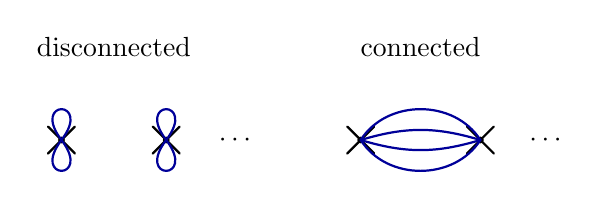
\begin{tikzpicture}[baseline=(current bounding box.center),scale=0.95]
  \node at (-1.0,1.25) {disconnected};
  \foreach \x in {-1.7,-0.3} {
    \draw[thick] (\x-0.18,-0.18) -- (\x+0.18,0.18);
    \draw[thick] (\x-0.18,0.18) -- (\x+0.18,-0.18);
    \fill (\x,0) circle (1.3pt);
    \draw[thick,blue!60!black]
      (\x,0) .. controls (\x-0.42,0.55) and (\x+0.42,0.55) .. (\x,0);
    \draw[thick,blue!60!black]
      (\x,0) .. controls (\x-0.42,-0.55) and (\x+0.42,-0.55) .. (\x,0);
  }
  \node at (0.65,0) {$\cdots$};

  \node at (3.1,1.25) {connected};
  \foreach \x in {2.3,3.9} {
    \draw[thick] (\x-0.18,-0.18) -- (\x+0.18,0.18);
    \draw[thick] (\x-0.18,0.18) -- (\x+0.18,-0.18);
    \fill (\x,0) circle (1.3pt);
  }
  \draw[thick,blue!60!black]
    (2.3,0) .. controls (2.65,0.55) and (3.55,0.55) .. (3.9,0);
  \draw[thick,blue!60!black]
    (2.3,0) .. controls (2.65,-0.55) and (3.55,-0.55) .. (3.9,0);
  \draw[thick,blue!60!black]
    (2.3,0) .. controls (2.9,0.18) and (3.3,0.18) .. (3.9,0);
  \draw[thick,blue!60!black]
    (2.3,0) .. controls (2.9,-0.18) and (3.3,-0.18) .. (3.9,0);
  \node at (4.8,0) {$\cdots$};
\end{tikzpicture}
\end{center}

More generally, at order $g^n$, each set of Wick contractions can be
represented by a graph. Suppose that the graph has $K$ connected components,
and that among them there are $m_\ell$ connected graphs containing
$\ell$ vertices each, for $\ell=1,2,3,\ldots$. Thus
\[
  \sum_{\ell\geq 1} m_\ell = K,
  \qquad
  \sum_{\ell\geq 1} \ell\,m_\ell = n.
\]
For a given partition of $n$, specified by the integers $m_\ell$, the
number of ways of grouping the $n$ vertices in this pattern is
\[
  \frac{n!}{\prod_{\ell\geq 1}(\ell!)^{m_\ell}m_\ell!}.
\]
If $G^{(\ell)}$ denotes the contribution from connected Wick contractions
of $\ell$ vertices, the total contribution of this partition is
\[
  \frac{1}{n!}\,
  \frac{n!}{\prod_{\ell\geq 1}(\ell!)^{m_\ell}m_\ell!}
  \prod_{\ell\geq 1}\bigl(G^{(\ell)}\bigr)^{m_\ell}
  =
  \prod_{\ell\geq 1}
  \frac{1}{m_\ell!}\left(\frac{1}{\ell!}G^{(\ell)}\right)^{m_\ell}.
\]
Summing over all $m_\ell$'s gives
\[
  \frac{Z_g}{Z_0}
  =
  \sum_{\{m_\ell\}}
  \prod_{\ell\geq 1}
  \frac{1}{m_\ell!}\left(\frac{1}{\ell!}G^{(\ell)}\right)^{m_\ell}
  =
  \prod_{\ell\geq 1}\exp\left(\frac{1}{\ell!}G^{(\ell)}\right)
  =
  \exp\left(\sum_{\ell\geq 1}\frac{1}{\ell!}G^{(\ell)}\right).
\]
Thus the logarithm of the partition function is the contribution from all
connected graphs.

As an example, one connected graph with three vertices contributes
\[
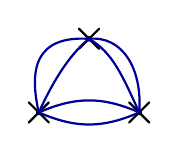
\begin{tikzpicture}[baseline=-0.45ex,scale=0.85]
  \coordinate (a) at (0,0);
  \coordinate (b) at (1.5,0);
  \coordinate (c) at (0.75,1.1);
  \foreach \p in {a,b,c} {
    \draw[thick] ($(\p)+(-0.15,-0.15)$) -- ($(\p)+(0.15,0.15)$);
    \draw[thick] ($(\p)+(-0.15,0.15)$) -- ($(\p)+(0.15,-0.15)$);
    \fill (\p) circle (1.2pt);
  }
  \draw[thick,blue!60!black] (a) .. controls (0.55,0.24) and (0.95,0.24) .. (b);
  \draw[thick,blue!60!black] (a) .. controls (0.55,-0.24) and (0.95,-0.24) .. (b);
  \draw[thick,blue!60!black] (b) .. controls (1.25,0.55) and (1.1,0.9) .. (c);
  \draw[thick,blue!60!black] (b) .. controls (1.55,0.65) and (1.25,1.15) .. (c);
  \draw[thick,blue!60!black] (c) .. controls (0.5,0.9) and (0.25,0.55) .. (a);
  \draw[thick,blue!60!black] (c) .. controls (-0.05,1.15) and (-0.15,0.65) .. (a);
\end{tikzpicture}
\quad
=
\frac{1}{3!}\left(-\frac{g}{4!}\right)^3
\int \dd\tau_1\,\dd\tau_2\,\dd\tau_3\,
\bigl(G_0(\tau_1,\tau_2)\bigr)^2
\bigl(G_0(\tau_2,\tau_3)\bigr)^2
\bigl(G_0(\tau_3,\tau_1)\bigr)^2.
\]
This still diverges like $\int\dd\tau$ times a constant.

\subsection{Ground State Energy from Vacuum Diagrams}

The interpretation of
\[
  Z=\int [\mathcal Dq]\,e^{-\int\dd\tau\,L^E}
\]
is
\[
  Z=\bra{q_f}e^{-HT}\ket{q_i},
\]
with boundary conditions at the initial and final imaginary times
$\tau=0,T$. Since these boundary conditions become unimportant as
$T\to\infty$,
\[
  \log Z=-E_0T+O(1),
\]
where $E_0$ is the ground-state energy. Indeed, perturbation theory gave
\[
  \log\left(\frac{Z_g}{Z_0}\right)
  =
  \sum_{\ell=1}^{\infty}\frac{1}{\ell!}G^{(\ell)},
\]
the sum of all connected Wick contractions of $\ell$ vertices.

One often absorbs the combinatorical factor $1/\ell!$ into the symmetry
factor of the graph itself. Each $G^{(\ell)}$ is of the form
$\int\dd\tau\,(\text{const.})$, and therefore is proportional to $T$.
Thus
\[
  E_0=-\lim_{T\to\infty}\frac{1}{T}\log Z
\]
is well-defined.

As already seen, at order $g$, $\ell=1$. The connected vacuum graph is
\[
  G^{(1)}
  =
  3\,
  
\begin{tikzpicture}[baseline=-0.5ex,scale=0.82]
    \draw[thick] (-0.15,-0.15) -- (0.15,0.15);
    \draw[thick] (-0.15,0.15) -- (0.15,-0.15);
    \fill (0,0) circle (1.2pt);
    \draw[thick,blue!60!black]
      (0,0) .. controls (-0.45,0.55) and (0.45,0.55) .. (0,0);
    \draw[thick,blue!60!black]
      (0,0) .. controls (-0.45,-0.55) and (0.45,-0.55) .. (0,0);
  \end{tikzpicture}
  =
  -\frac{g}{8}\int\dd\tau\,\bigl(G_0(\tau,\tau)\bigr)^2.
\]
Recall that
\[
  G_0(\tau_1,\tau_2)=\frac{1}{2\omega}e^{-\omega|\tau_{12}|},
  \qquad
  G_0(\tau,\tau)=\frac{1}{2\omega}.
\]
Thus, setting $\omega=1$ when desired,
\[
  \Delta E_0
  =
  \frac{g}{8}\left(\frac{1}{2\omega}\right)^2+O(g^2).
\]

This agrees with Hamiltonian perturbation theory. Writing
\[
  H=
  \underbrace{\frac{\hat p^2}{2}+\frac{\hat q^2}{2}}_{H_0}
  +
  \underbrace{\frac{g}{4!}\hat q^4}_{H_1},
\]
and letting $\ket{\psi_0}$ be the ground state of $H_0$, to leading order
in $g$,
\[
  \Delta E_0\simeq
  \bra{\psi_0}H_1\ket{\psi_0}
  =
  \frac{g}{4!}\left\langle q^4\right\rangle_0
  =
  \frac{g}{4!}\cdot\frac{3}{4}
  =
  \frac{g}{32}.
\]

\subsection{The Two-Point Function and One-Particle-Irreducible Graphs}

\newcommand{\qftFreeProp}{%
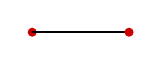
\begin{tikzpicture}[baseline=-0.55ex,scale=0.82]
  \fill[red!80!black] (0,0) circle (2pt);
  \draw[thick] (0,0) -- (1.5,0);
  \fill[red!80!black] (1.5,0) circle (2pt);
\end{tikzpicture}}
\newcommand{\qftTadpoleProp}{%
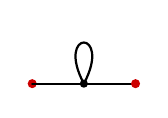
\begin{tikzpicture}[baseline=-0.55ex,scale=0.82]
  \fill[red!80!black] (0,0) circle (2pt);
  \draw[thick] (0,0) -- (1.6,0);
  \fill[red!80!black] (1.6,0) circle (2pt);
  \fill (0.8,0) circle (1.8pt);
  \draw[thick] (0.8,0) .. controls (0.35,0.85) and (1.25,0.85) .. (0.8,0);
\end{tikzpicture}}
\newcommand{\qftDoubleTadpoleProp}{%
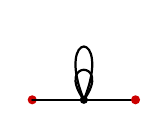
\begin{tikzpicture}[baseline=-0.55ex,scale=0.82]
  \fill[red!80!black] (0,0) circle (2pt);
  \draw[thick] (0,0) -- (1.6,0);
  \fill[red!80!black] (1.6,0) circle (2pt);
  \fill (0.8,0) circle (1.8pt);
  \draw[thick] (0.8,0) .. controls (0.35,0.62) and (1.25,0.62) .. (0.8,0);
  \draw[thick] (0.8,0) .. controls (0.35,1.1) and (1.25,1.1) .. (0.8,0);
\end{tikzpicture}}
\newcommand{\qftTwoVertexTadpoles}{%
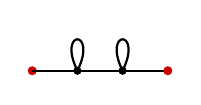
\begin{tikzpicture}[baseline=-0.55ex,scale=0.82]
  \fill[red!80!black] (0,0) circle (2pt);
  \draw[thick] (0,0) -- (2.1,0);
  \fill[red!80!black] (2.1,0) circle (2pt);
  \foreach \x in {0.7,1.4} {
    \fill (\x,0) circle (1.8pt);
    \draw[thick] (\x,0) .. controls (\x-0.32,0.65) and (\x+0.32,0.65) .. (\x,0);
  }
\end{tikzpicture}}
\newcommand{\qftBubbleProp}{%
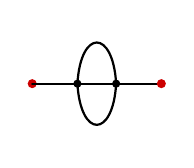
\begin{tikzpicture}[baseline=-0.55ex,scale=0.82]
  \fill[red!80!black] (0,0) circle (2pt);
  \draw[thick] (0,0) -- (2.0,0);
  \fill[red!80!black] (2.0,0) circle (2pt);
  \fill (0.7,0) circle (1.8pt);
  \fill (1.3,0) circle (1.8pt);
  \draw[thick] (0.7,0) .. controls (0.75,0.85) and (1.25,0.85) .. (1.3,0);
  \draw[thick] (0.7,0) .. controls (0.75,-0.85) and (1.25,-0.85) .. (1.3,0);
\end{tikzpicture}}
\newcommand{\qftBlobProp}{%
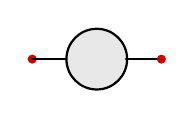
\begin{tikzpicture}[baseline=-0.55ex,scale=0.82]
  \fill[red!80!black] (0,0) circle (2pt);
  \draw[thick] (0,0) -- (0.55,0);
  \draw[fill=gray!18,thick] (1.0,0) circle (0.47);
  \draw[thick] (1.45,0) -- (2.0,0);
  \fill[red!80!black] (2.0,0) circle (2pt);
\end{tikzpicture}}
\newcommand{\qftOnePI}{%
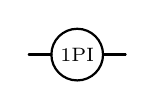
\begin{tikzpicture}[baseline=-0.55ex,scale=0.82]
  \draw[thick] (0,0) -- (0.35,0);
  \draw[thick] (1.15,0) -- (1.5,0);
  \draw[thick] (0.75,0) circle (0.4);
  \node at (0.75,0) {\scriptsize 1PI};
\end{tikzpicture}}
\newcommand{\qftOnePIChain}{%
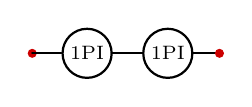
\begin{tikzpicture}[baseline=-0.55ex,scale=0.82]
  \fill[red!80!black] (0,0) circle (2pt);
  \draw[thick] (0,0) -- (0.45,0);
  \draw[thick] (0.85,0) circle (0.38);
  \node at (0.85,0) {\scriptsize 1PI};
  \draw[thick] (1.23,0) -- (1.72,0);
  \draw[thick] (2.1,0) circle (0.38);
  \node at (2.1,0) {\scriptsize 1PI};
  \draw[thick] (2.48,0) -- (2.9,0);
  \fill[red!80!black] (2.9,0) circle (2pt);
\end{tikzpicture}}

Next we turn to
\[
  \bra{0}\hat q(\tau)\hat q(0)\ket{0},
  \qquad \tau>0,
\]
which is
\[
  \frac{1}{Z}\int[\mathcal Dq]\,
  e^{-\int\dd\tau\,L^E}\,q(\tau)q(0).
\]
Expanding in \(g\),
\[
  \bra{0}\hat q(\tau)\hat q(0)\ket{0}
  =
  \frac{1}{Z}
  \left\langle
    q(\tau)q(0)
    \sum_{n=0}^{\infty}
    \frac{1}{n!}
    \left(
      -\frac{g}{4!}\int\dd\tau'\,q^4(\tau')
    \right)^n
  \right\rangle_0.
\]
This is computed by summing all possible Wick contractions. A typical term
has one connected component containing the external insertions, together
with other disconnected components:
\begin{center}
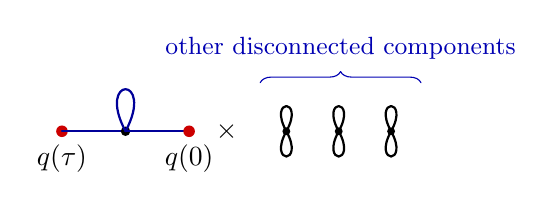
\begin{tikzpicture}[scale=0.95]
  \fill[red!80!black] (0,0) circle (2.2pt);
  \node[below] at (0,-0.05) {$q(\tau)$};
  \draw[thick,blue!60!black] (0,0) -- (0.85,0);
  \fill (0.85,0) circle (1.8pt);
  \draw[thick,blue!60!black] (0.85,0) .. controls (0.45,0.75) and (1.25,0.75) .. (0.85,0);
  \draw[thick,blue!60!black] (0.85,0) -- (1.7,0);
  \fill[red!80!black] (1.7,0) circle (2.2pt);
  \node[below] at (1.7,-0.05) {$q(0)$};
  \node at (2.2,0) {$\times$};
  \draw[decorate,decoration={brace,amplitude=4pt},blue!70!black]
    (2.65,0.65) -- (4.8,0.65)
    node[midway,above=5pt] {\small other disconnected components};
  \foreach \x in {3.0,3.7,4.4} {
    \draw[thick] (\x,0) .. controls (\x-0.25,0.45) and (\x+0.25,0.45) .. (\x,0);
    \draw[thick] (\x,0) .. controls (\x-0.25,-0.45) and (\x+0.25,-0.45) .. (\x,0);
    \fill (\x,0) circle (1.5pt);
  }
\end{tikzpicture}
\end{center}
The sum factorizes into a connected graph joining \(q(\tau)\) to \(q(0)\)
times disconnected vacuum graphs. The disconnected vacuum graphs cancel
against the factor \(1/Z\), leaving
\[
  \bra{0}\hat q(\tau)\hat q(0)\ket{0}
  =
  \qftFreeProp
  \;+\;
  \qftTadpoleProp
  \;+\;
  \qftTwoVertexTadpoles
  \;+\;
  \qftDoubleTadpoleProp
  \;+\;
  \qftBubbleProp
  \;+\;\cdots .
\]

The same path integral expression computes
\(\bra{0}\hat q(0)\hat q(\tau)\ket{0}\) for \(\tau<0\). We can write the
Euclidean Green function as
\[
  G_E(\tau)=\langle q(\tau)q(0)\rangle
  =
  \begin{cases}
    \bra{0}\hat q(\tau)\hat q(0)\ket{0}, & \tau>0,\\
    \bra{0}\hat q(0)\hat q(\tau)\ket{0}, & \tau<0.
  \end{cases}
\]
At zeroth order,
\[
  \qftFreeProp
  =
  G_0(\tau)
  =
  \frac{1}{2}e^{-|\tau|}
  =
  \int\frac{\dd k}{2\pi}\,\widetilde G_0(k)e^{ik\tau},
  \qquad
  \widetilde G_0(k)=\frac{1}{k^2+1}.
\]
At order \(g\), the connected correction is
\[
  \qftTadpoleProp
  =
  -\frac{g}{2}
  \int\dd\tau'\,
  G_0(\tau-\tau')G_0(\tau')G_0(0).
\]
It is convenient to evaluate this using the Fourier transform:
\[
\begin{aligned}
  \qftTadpoleProp
  &=
  -\frac{g}{2}
  \int\dd\tau'
  \int\frac{\dd k}{2\pi}\frac{\dd k'}{2\pi}\frac{\dd k''}{2\pi}\,
  \widetilde G_0(k)\widetilde G_0(k')\widetilde G_0(k'')\,
  e^{ik(\tau-\tau')+ik'\tau'}                                      \\
  &=
  -\frac{g}{2}\cdot\frac{1}{2}
  \int\frac{\dd k}{2\pi}\,
  \frac{e^{ik\tau}}{(k^2+1)^2}.
\end{aligned}
\]
At order \(g^2\), the diagrams
\[
  \qftTwoVertexTadpoles
  \qquad
  \qftDoubleTadpoleProp
  \qquad
  \qftBubbleProp
\]
are left as a Problem Set 2 calculation.

The full perturbative two-point function has the structure
\[
  \qftBlobProp
  =
  \qftFreeProp
  \;+\;
  \qftOnePI
  \;+\;
  \qftOnePIChain
  \;+\;\cdots .
\]
Here ``1PI'' means one-particle-irreducible: the graph remains connected
after cutting any one propagator. In momentum space this gives
\[
  G(\tau)
  =
  \int\frac{\dd k}{2\pi}\,e^{ik\tau}\,
  \widetilde G_0(k)
  \sum_{n=0}^{\infty}\bigl(\widetilde G_0(k)\Sigma(k)\bigr)^n
  =
  \int\frac{\dd k}{2\pi}\,e^{ik\tau}\,
  \frac{1}{k^2+1-\Sigma(k)}.
\]
The self-energy \(\Sigma(k)\) is the sum of amputated 1PI graphs, not
including the external propagators. To second order,
\[
  \Sigma(k)
  =
  -\frac{g}{4}
  +
  \frac{g^2}{8}
  \left(
    \frac{1}{4}+\frac{1}{k^2+9}
  \right)
  +O(g^3).
\]
Therefore
\[
  \langle q(\tau)q(0)\rangle
  \equiv G(\tau)
  =
  \int\frac{\dd k}{2\pi}\,\widetilde G(k)e^{ik\tau},
\]
with
\[
  \widetilde G(k)
  =
  \frac{1}{
    k^2+1+\frac{g}{4}
    -\frac{g^2}{8}\left(\frac{1}{4}+\frac{1}{k^2+9}\right)
    +O(g^3)
  }.
\]

On the other hand, for \(\tau>0\) we know that
\[
  \bra{0}\hat q(\tau)\hat q(0)\ket{0}
  =
  \sum_n
  \left|\bra{n}\hat q(0)\ket{0}\right|^2
  e^{-(E_n-E_0)\tau}.
\]
Consider the analytic continuation of \(\widetilde G(k)\) to the complex
\(k\)-plane:
\begin{center}
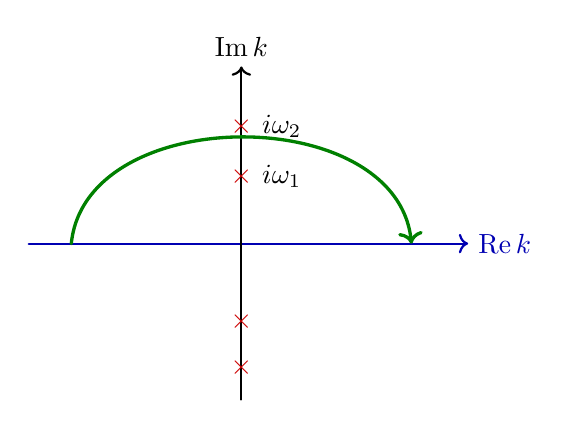
\begin{tikzpicture}[scale=0.9]
  \draw[->,thick,blue!70!black] (-3.0,0) -- (3.2,0) node[right] {$\operatorname{Re}k$};
  \draw[->,thick] (0,-2.2) -- (0,2.5) node[above] {$\operatorname{Im}k$};
  \draw[very thick,green!50!black,->]
    (-2.4,0) .. controls (-2.2,2.0) and (2.2,2.0) .. (2.4,0);
  \foreach \y/\lab in {0.95/{i\omega_1},1.65/{i\omega_2}} {
    \node[red!80!black] at (0,\y) {$\times$};
    \node[right=4pt] at (0,\y) {$\lab$};
  }
  \node[red!80!black] at (0,-1.1) {$\times$};
  \node[red!80!black] at (0,-1.75) {$\times$};
\end{tikzpicture}
\end{center}
Closing the contour at infinity in the upper half-plane,
\[
  \int\frac{\dd k}{2\pi}\,\widetilde G(k)e^{ik\tau}
  =
  i\sum_n e^{-\omega_n\tau}
  \operatorname*{Res}_{k\to i\omega_n}\widetilde G(k),
  \qquad
  \omega_n=E_n-E_0.
\]
For example, from the expression above for \(\widetilde G(k)\), the first
pole is expected near \(k\simeq i\), and one finds
\[
  \omega_1
  =
  1+\frac{g}{8}-\frac{g^2}{32}+O(g^3),
\]
which agrees with Hamiltonian perturbation theory at second order.

\subsection{Derivative Interactions and the Measure}

Here is a closely related example which is more subtle. Take
\[
  L=\frac12\dot q^2-\frac12 q^2-\frac{g}{8}q^2\dot q^2 .
\]
The canonical momentum is
\[
  p=\frac{\partial L}{\partial \dot q}
    =\dot q\left(1-\frac{g}{4}q^2\right),
\]
and therefore
\[
  H=\dot q p-L
   =\frac12\left(1-\frac{g}{4}q^2\right)^{-1}p^2+\frac12q^2 .
\]
This expression already suggests a possible operator-ordering ambiguity in
quantization.

One can also consider a change of variable
\[
  \dot y=\left(1-\frac{g}{4}q^2\right)^{1/2}\dot q,
  \qquad
  y=q-\frac{g}{24}q^3+\cdots .
\]
In terms of the new variable the Lagrangian takes the form
\[
  L=\frac12\dot y^2-V(y),
  \qquad
  V(y)=\frac12 y^2+\frac{g}{24}y^4+\cdots ,
\]
which is the anharmonic oscillator up to corrections of order \(g^2\) in the
potential. We will instead insist on working with the \(q\)-variable in the
path integral and see what happens.

The Euclidean Lagrangian is
\[
  L^E
  =\frac12(\partial_\tau q)^2+\frac12q^2
    -\frac{g}{8}q^2(\partial_\tau q)^2 .
\]
It is useful to write the interaction term as
\[
  q^2(\partial_\tau q)^2
  =\frac13\,\partial_\tau\!\left(q^3\partial_\tau q\right)
    -\frac13\,q^3\partial_\tau^2q,
\]
so that, up to a total derivative,
\[
  L^E
  =\frac12(\partial_\tau q)^2+\frac12q^2
    +\frac{g}{24}q^3\partial_\tau^2q .
\]

To first order in \(g\), the two-point function is
\[
\begin{aligned}
  \langle q(\tau)q(0)\rangle
  &=G_0(\tau)
    +\frac{g}{8}\int \dd \tau'\,
      \big\langle q(\tau)q(0)\,q(\tau')^2
      \big(\partial_{\tau'}q(\tau')\big)^2\big\rangle_0+\cdots .
\end{aligned}
\]
The possible Wick contractions are represented schematically by
\[
\begin{tikzpicture}[baseline=(current bounding box.center), x=1cm, y=1cm]
  \coordinate (a) at (0,0);
  \coordinate (b) at (1.2,0);
  \coordinate (c) at (2.4,0);
  \draw (a) node[below] {\(\tau\)};
  \draw (c) node[below] {\(0\)};
  \draw (a) -- (b) -- (c);
  \draw (b) circle[radius=.28];
  \draw[blue, thick] ($(b)+(-.08,.28)$) -- ($(b)+(-.08,.48)$);
  \draw[blue, thick] ($(b)+(.08,.28)$) -- ($(b)+(.08,.48)$);
  \node at (b) [below=.38cm] {\(\tau'\)};

  \node at (3.1,0) {\(+\)};

  \coordinate (d) at (3.8,0);
  \coordinate (e) at (5.0,0);
  \coordinate (f) at (6.2,0);
  \draw (d) -- (e) -- (f);
  \draw (e) circle[radius=.28];
  \draw[blue, thick] ($(e)+(-.22,.15)$) -- ($(e)+(-.35,.32)$);
  \draw[blue, thick] ($(e)+(.22,.15)$) -- ($(e)+(.35,.32)$);
  \node at (e) [below=.38cm] {\(\tau'\)};

  \node at (6.9,0) {\(+\)};

  \coordinate (g) at (7.6,0);
  \coordinate (h) at (8.8,0);
  \coordinate (i) at (10.0,0);
  \draw (g) -- (h) -- (i);
  \draw (h) .. controls +(70:.55) and +(110:.55) .. (h);
  \draw[blue, thick] ($(h)+(-.18,.2)$) -- ($(h)+(-.35,.38)$);
  \draw[blue, thick] ($(h)+(.18,.2)$) -- ($(h)+(.35,.38)$);
  \node at (h) [below=.38cm] {\(\tau'\)};

  \node at (10.7,0) {\(+\cdots\)};
\end{tikzpicture}
\]
where the blue marks indicate derivatives acting on the corresponding
propagators.

One of these terms gives
\[
  2\cdot\frac{g}{8}\int\dd\tau'\,
  G_0(\tau-\tau')G_0(\tau')\,\bigl(-\partial^2G_0(0)\bigr)
  =
  \frac{g}{4}\int\dd\tau'\,
  G_0(\tau-\tau')G_0(\tau')\,\bigl(-\partial^2G_0(0)\bigr).
\]
Since
\[
  G_0(\tau)=\frac12e^{-|\tau|},
\]
the factor \(-\partial^2G_0(0)\) is divergent. The other contributions are
finite. For example,
\[
  \frac{g}{4}
  \int\frac{\dd k}{2\pi}\,
    \frac{e^{ik\tau}}{(k^2+1)^2}\,k^2
  \int\frac{\dd k'}{2\pi}\,\frac{1}{k'^2+1},
\]
and
\[
  -\frac{g}{2}
  \int\frac{\dd k}{2\pi}\,
    \frac{e^{ik\tau}}{(k^2+1)^2}\,ik
  \int\frac{\dd k'}{2\pi}\,\frac{ik'}{k'^2+1}=0
\]
by symmetry. The remaining diagrams are similar.

The divergence comes from the integral at large momentum. Its origin lies in
the definition of the path integral measure. Writing
\[
  q(\tau)=\int\frac{\dd k}{2\pi}\,\widetilde q(k)e^{ik\tau},
\]
the formal measure is
\[
  [Dq]=\prod_k \dd \widetilde q_k .
\]
To define it, introduce a cutoff
\[
  [Dq]_\Lambda=\prod_{|k|<\Lambda}\dd \widetilde q_k .
\]
This cuts off the loop integral by \(|k'|<\Lambda\); only after computing do
we ask whether \(\Lambda\to\infty\) can be taken.

With this regularization,
\[
  \widetilde G(k)
  =\frac{1}{k^2+1-\Sigma(k)} ,
\]
and, to first order in \(g\),
\[
\begin{aligned}
  \Sigma_\Lambda(k)
  &=
  \frac{g}{4}\int_{|k'|<\Lambda}
       \frac{\dd k'}{2\pi}\,\frac{k'^2}{k'^2+1}
  +\frac{g}{4}k^2
       \int_{|k'|<\Lambda}
       \frac{\dd k'}{2\pi}\,\frac{1}{k'^2+1}
  +O(g^2)\\
  &=
  \frac{g}{4}\left(
    \frac{\Lambda}{\pi}+\frac{k^2}{2}-\frac12+O(\Lambda^{-1})
  \right)+O(g^2).
\end{aligned}
\]

What is the interpretation of the \(\Lambda\to\infty\) limit? There is
nothing wrong with the quantum-mechanical Hamiltonian
\[
  H=\frac12\left(1-\frac{g}{4}q^2\right)^{-1}p^2+\frac12q^2
\]
at least for \(g<0\), aside from the operator-ordering ambiguity mentioned
above. To understand what is going on, restore the \(\hbar\)-dependence:
\[
  Z=\int[Dq]\,
  \exp\left[-\frac{1}{\hbar}\int\dd\tau\,L^E\right].
\]
Then
\[
  \widetilde G(k)=\frac{\hbar}{k^2+1-\Sigma(k)}
\]
and
\[
  \Sigma_\Lambda(k)
  =\frac{\hbar g}{4}\left(
    \frac{\Lambda}{\pi}+\frac{k^2}{2}-\frac12+O(\Lambda^{-1})
  \right)+O(\hbar^2g^2).
\]

Indeed, if we include a counterterm
\[
  \Delta L^E=C\,g\,\hbar\,\frac{q^2}{2},
\]
the one-particle-irreducible two-point function receives an extra
contribution \(-C g\hbar\). Thus
\[
  \Sigma_\Lambda(k)
  =
  \hbar g\left(
    \frac{k^2}{8}+\frac{\Lambda}{4\pi}
    -\frac18-C+O(\Lambda^{-1})
  \right)+O(g^2).
\]
The path integral is only defined once a regularization has been specified.
Choosing
\[
  C=\frac{\Lambda}{4\pi}+\text{finite}
\]
and taking \(\Lambda\to\infty\) at the end gives a finite answer for
\(\Sigma(k)\). The finite part of \(C\) represents an ambiguity in
quantization, namely the possibility of adjusting the quantum Hamiltonian by a
term of order \(\hbar\).

The pole of
\[
  \widetilde G(k)=\frac{\hbar}{k^2+1-\Sigma(k)}
\]
at \(k=i\omega_1\) gives
\[
  \omega_1
  =
  1+\hbar g\left(
    -\frac{\Lambda}{8\pi}+\frac{C}{2}+\frac18
  \right)+O(g^2)
  =E_1-E_0 .
\]
This energy gap is an unambiguous physical observable, regardless of the
interpretation of \(q(\tau)\). The counterterms, together with the
regularization scheme, should be viewed as part of the definition of the path
integral. Fixing the finite part of the counterterms requires additional
physical input, for example symmetries of the quantum Hamiltonian. In general
quantum mechanics anything can appear in \(H\); in quantum field theory,
Poincare symmetry and causality are highly restrictive.

\section{A Manifestly Relativistic Theory of Fields}

In classical mechanics the dynamical variables are \(q^i(t)\). In a field
theory they are replaced by fields
\[
  q^i(t)\quad\leadsto\quad \phi(t,\vec x),
\]
where \(\vec x\in \mathbb R^{D-1}\) is viewed as a continuous label for the
variables. We will write
\[
  x^\mu=(x^0,\vec x),\qquad x^0=t,
\]
interchangeably.

The action is
\[
  S=\int \dd t\,\dd^{D-1}\vec x\,
  \mathcal L\bigl[\phi(x),\partial_\mu\phi(x),\ldots\bigr]
  =
  \int \dd^D x\,
  \mathcal L\bigl[\phi(x),\partial_\mu\phi(x),\ldots\bigr],
\]
where \(\mathcal L\) is the Lagrangian density. The equation of motion is
\[
  \frac{\delta S}{\delta\phi(x)}=0.
\]
Assume for now that \(\mathcal L\) depends on \(\phi(x)\) only through
\(\phi(x)\) and its first-order derivatives \(\partial_\mu\phi(x)\). Then
\[
\begin{aligned}
  \delta S
  &=
  \int\dd^D x\left[
    \delta\phi(x)\frac{\partial\mathcal L}{\partial\phi(x)}
    +\delta\partial_\mu\phi(x)
      \frac{\partial\mathcal L}{\partial(\partial_\mu\phi(x))}
  \right]\\
  &=
  \int\dd^D x\,\delta\phi(x)\left[
    \frac{\partial\mathcal L}{\partial\phi(x)}
    -\partial_\mu
      \frac{\partial\mathcal L}{\partial(\partial_\mu\phi(x))}
  \right],
\end{aligned}
\]
where the second line follows by integration by parts. The Euler-Lagrange
equation is therefore
\[
  \frac{\partial\mathcal L}{\partial\phi(x)}
  -\partial_\mu
   \frac{\partial\mathcal L}{\partial(\partial_\mu\phi(x))}
  =0 .
\]

\subsection{The Free Massive Scalar Field}

For a free massive scalar field,
\[
  \mathcal L
  =
  \frac12(\partial_t\phi)^2
  -\frac12\sum_{i=1}^{D-1}(\partial_{x^i}\phi)^2
  -\frac12m^2\phi^2 .
\]
With the convention
\[
  \eta^{\mu\nu}=\operatorname{diag}(-1,1,\ldots,1),
\]
this can be written as
\[
  \mathcal L
  =
  -\frac12(\partial_\mu\phi)^2-\frac12m^2\phi^2 .
\]
The Euler-Lagrange equation gives the Klein-Gordon equation
\[
  \partial^\mu\partial_\mu\phi-m^2\phi=0 .
\]

The general solution can be written as a Fourier transform
\[
  \phi(x)=\int \dd^D k\, f(k)e^{ik\cdot x}.
\]
Using
\[
  k\cdot x=\vec k\cdot\vec x-k^0x^0,
\]
the equation of motion requires
\[
  (k^2+m^2)f(k)=0.
\]
Thus \(f(k)\) is a distribution supported on the mass shell
\[
  k^2+m^2=0,
  \qquad
  k^0=\pm\sqrt{\vec k^2+m^2}.
\]
Equivalently,
\[
  \phi(x)
  =
  \int \dd^{D-1}\vec k\,
  \left[
    \widetilde f(\vec k)\,
      e^{i\vec k\cdot\vec x-i\omega_{\vec k}x^0}
    +
    \widetilde f^*(\vec k)\,
      e^{-i\vec k\cdot\vec x+i\omega_{\vec k}x^0}
  \right],
\]
where
\[
  \omega_{\vec k}=\sqrt{\vec k^2+m^2}.
\]

The initial-value problem is: given
\(\phi(t=0,\vec x)\) and \(\partial_t\phi(t=0,\vec x)\), determine
\(\phi(t>0,\vec x)\). At \(t=0\),
\[
  \phi(t=0,\vec x)
  =
  \int\dd^{D-1}\vec k\,e^{i\vec k\cdot\vec x}
  \left[
    \widetilde f(\vec k)+\widetilde f^*(-\vec k)
  \right],
\]
and
\[
  \partial_t\phi(t=0,\vec x)
  =
  \int\dd^{D-1}\vec k\,e^{i\vec k\cdot\vec x}
  (-i\omega_{\vec k})
  \left[
    \widetilde f(\vec k)-\widetilde f^*(-\vec k)
  \right].
\]
Together these determine \(\widetilde f(\vec k)\) and
\(\widetilde f^*(-\vec k)\), and hence \(\phi(x)\) at any time
\(t\equiv x^0\).

A relativistic quantum theory may be constructed by quantizing the classical
field theory. There are two approaches.

\begin{enumerate}[label=(\arabic*)]
\item Canonical quantization: construct a Hilbert space using wave functions
  in the variables \(\phi(\vec x,t=0)\), together with the Hamiltonian \(H\).
\item Path integral:
  \[
    Z=\int[D\phi]\,
    e^{\frac{i}{\hbar}S[\phi]} .
  \]
  To make sense of the functional measure typically requires regularization.
\end{enumerate}

\subsection{Canonical Formalism}

The Lagrangian is
\[
  L=\int\dd^{D-1}\vec x\,
  \mathcal L[\phi,\partial_\mu\phi].
\]
For the free scalar field,
\[
  L=\int\dd^{D-1}\vec x\,
  \left[
    -\frac12(\partial_\mu\phi)^2-\frac12m^2\phi^2
  \right].
\]
The dynamical variable is \(\phi(t,\vec x)\). The time \(t\) is the evolution
parameter, while \(\vec x\) is just a continuous label. Thus the canonical
coordinates are the values of \(\phi(t,\vec x)\).

The conjugate canonical momentum density is
\[
  \Pi(t,\vec x)
  =
  \frac{\partial\mathcal L}{\partial\dot\phi(t,\vec x)}
  =
  \dot\phi(t,\vec x)
\]
in the present example. The classical Hamiltonian is
\[
  H=\int\dd^{D-1}\vec x\,\mathcal H,
\]
with Hamiltonian density
\[
  \mathcal H
  =
  \Pi(t,\vec x)\dot\phi(t,\vec x)-\mathcal L.
\]
For the free scalar field,
\[
  \mathcal H
  =
  \frac12\dot\phi^2+\frac12(\partial_{\vec x}\phi)^2+\frac12m^2\phi^2
  =
  \frac12\Pi^2+\frac12(\partial_{\vec x}\phi)^2+\frac12m^2\phi^2.
\]
In terms of \((\phi,\Pi)\), the \(\Pi^2\) term is kinetic and the remaining
terms are potential.

Omitting the time argument, the Poisson brackets are
\[
  \{\phi(\vec x),\phi(\vec x')\}=0=\{\Pi(\vec x),\Pi(\vec x')\},
\]
and
\[
  \{\Pi(\vec x),\phi(\vec x')\}
  =\delta^{D-1}(\vec x-\vec x').
\]
For two functionals,
\[
  \{F,G\}
  =
  \int\dd^{D-1}\vec x\left[
    \frac{\delta F}{\delta\Pi(\vec x)}
    \frac{\delta G}{\delta\phi(\vec x)}
    -
    \frac{\delta F}{\delta\phi(\vec x)}
    \frac{\delta G}{\delta\Pi(\vec x)}
  \right].
\]
The equations of motion are
\[
  \dot F=\{H,F\}
\]
as usual.

Quantization promotes \(\phi(t,\vec x)\) and \(\Pi(t,\vec x)\) to operators
\[
  \hat\phi(t,\vec x),\qquad \hat\Pi(t,\vec x),
\]
which obey equal-time commutators
\[
  [\hat\phi(t,\vec x),\hat\phi(t,\vec x')]
  =0=
  [\hat\Pi(t,\vec x),\hat\Pi(t,\vec x')],
\]
and
\[
  [\hat\phi(t,\vec x),\hat\Pi(t,\vec x')]
  =
  i\hbar\,\delta^{D-1}(\vec x-\vec x').
\]

It is convenient to perform a spatial Fourier transform, say at \(t=0\):
\[
  \hat\phi(t=0,\vec x)
  =
  \int
  \frac{\dd^{D-1}\vec k}
  {\sqrt{(2\pi)^{D-1}2\nu(\vec k)}}\,
  \bigl(a_{\vec k}+a^\dagger_{-\vec k}\bigr)
  e^{i\vec k\cdot\vec x}.
\]
For now the denominator is just a normalization convention, and the
combination \(a_{\vec k}+a^\dagger_{-\vec k}\) can be viewed as a definition
of the \(a\)'s. Similarly,
\[
  \hat\Pi(t=0,\vec x)
  =
  \int
  \frac{\dd^{D-1}\vec k}
  {\sqrt{(2\pi)^{D-1}2\nu(\vec k)}}\,
  \bigl(-i\nu(\vec k)\bigr)
  \bigl(a_{\vec k}-a^\dagger_{-\vec k}\bigr)
  e^{i\vec k\cdot\vec x}.
\]

It follows from the canonical commutation relation that
\[
  [a_{\vec k}+a^\dagger_{-\vec k},
   a_{\vec k'}+a^\dagger_{-\vec k'}]=0,
\]
\[
  [a_{\vec k}-a^\dagger_{-\vec k},
   a_{\vec k'}-a^\dagger_{-\vec k'}]=0,
\]
and
\[
  [a_{\vec k}+a^\dagger_{-\vec k},
   a_{\vec k'}-a^\dagger_{-\vec k'}]
  =
  -2\,\delta^{D-1}(\vec k+\vec k').
\]
Also,
\[
  [a_{\vec k}-a^\dagger_{-\vec k},
   a_{\vec k'}+a^\dagger_{-\vec k'}]
  =
  2\,\delta^{D-1}(\vec k+\vec k').
\]
The fact that \(a^\dagger_{\vec k}\) is the Hermitian conjugate of
\(a_{\vec k}\) ensures that \(\hat\phi\) and \(\hat\Pi\) are Hermitian.

These commutation relations are equivalent to
\[
  [a_{\vec k},a_{\vec k'}]=0=[a^\dagger_{\vec k},a^\dagger_{\vec k'}],
  \qquad
  [a_{\vec k},a^\dagger_{\vec k'}]
  =
  \delta^{D-1}(\vec k-\vec k').
\]
These are precisely the commutation relations obeyed by particle annihilation
and creation operators. However, this does not mean that \(a_{\vec k}\) and
\(a^\dagger_{\vec k}\) are actually annihilation and creation operators: we
have not used the Hamiltonian, nor specified \(\nu(\vec k)\).

Indeed, had we defined \(b_{\vec k}\) and \(b^\dagger_{\vec k}\) by
\[
  b_{\vec k}+b^\dagger_{-\vec k}
  =
  \lambda(\vec k)\bigl(a_{\vec k}+a^\dagger_{-\vec k}\bigr),
  \qquad
  b_{\vec k}-b^\dagger_{-\vec k}
  =
  \lambda(\vec k)^{-1}
  \bigl(a_{\vec k}-a^\dagger_{-\vec k}\bigr),
\]
then \(b_{\vec k}\) and \(b^\dagger_{\vec k}\) would also obey the
commutation relations of annihilation and creation operators. Explicitly,
\[
  b_{\vec k}
  =
  \frac{\lambda+\lambda^{-1}}{2}a_{\vec k}
  +
  \frac{\lambda-\lambda^{-1}}{2}a^\dagger_{-\vec k},
\]
which is a Bogoliubov transformation. Is the vacuum state \(\ket{\Omega}\)
annihilated by \(a_{\vec k}\)? If so,
\[
  b_{\vec k}\ket{\Omega}\ne 0
  \qquad
  (\lambda\ne 1).
\]

Now consider the Hamiltonian of the free scalar field. Substituting the
Fourier expansions into \(\hat H_0\) gives
\[
\begin{aligned}
  \hat H_0
  =
  \int\dd^{D-1}\vec k\,
  \Bigg[
  &\frac12\frac{\nu(\vec k)}{2}
  \bigl(a_{\vec k}-a^\dagger_{-\vec k}\bigr)
  \bigl(a_{-\vec k}-a^\dagger_{\vec k}\bigr)\\
  &+
  \frac12\frac{1}{2\nu(\vec k)}
  (\vec k^2+m^2)
  \bigl(a_{\vec k}+a^\dagger_{-\vec k}\bigr)
  \bigl(a_{-\vec k}+a^\dagger_{\vec k}\bigr)
  \Bigg].
\end{aligned}
\]
Setting
\[
  \nu(\vec k)=\omega_{\vec k},
  \qquad
  \omega_{\vec k}\equiv\sqrt{\vec k^2+m^2},
\]
diagonalizes the Hamiltonian:
\[
  \hat H_0
  =
  \int\dd^{D-1}\vec k\,
  \omega_{\vec k}
  \left(
    a^\dagger_{\vec k}a_{\vec k}
    +\frac12\delta^{D-1}(0)
  \right).
\]
The term proportional to \(\delta^{D-1}(0)\) is the normal-ordering constant,
and it reflects an ordering ambiguity. The true quantum Hamiltonian must be a
well-defined self-adjoint operator. We will remove the normal-ordering
constant by a constant shift of \(\hat H\). This will be justified as a
consequence of assuming Poincare invariance of the vacuum \(\ket{\Omega}\).

Using
\[
  \dot F=\frac{i}{\hbar}[\hat H,F],
\]
we can determine the time-dependence of \(\hat\phi(t,\vec x)\) and
\(\hat\Pi(t,\vec x)\). For example,
\[
  \hat\phi(t,\vec x)
  =
  \int
  \frac{\dd^{D-1}\vec k}
  {\sqrt{(2\pi)^{D-1}2\omega_{\vec k}}}
  \left(
    a_{\vec k}e^{ik\cdot x}
    +a^\dagger_{\vec k}e^{-ik\cdot x}
  \right),
\]
where
\[
  k\cdot x=\vec k\cdot\vec x-\omega_{\vec k}t .
\]

As we have seen previously, \(\hat\phi(x)\) is a Poincare-covariant local
operator:
\[
  \hat\phi(\Lambda x+a)
  =
  U(\Lambda,a)\hat\phi(x)U(\Lambda,a)^{-1}.
\]
The vacuum obeys
\[
  a_{\vec k}\ket{\Omega}=0
  \qquad \forall\,\vec k,
\]
and
\[
  H\ket{\Omega}=0.
\]

\section{Symmetries and Noether's Theorem}

A symmetry of a classical field theory is a transformation under which the
action is invariant. We write the infinitesimal transformation of the field as
\[
  \phi(x)\sim \phi'(x)=\phi(x)+\epsilon\,\delta\phi(x),
\]
where \(\epsilon\) is an infinitesimal parameter and \(\delta\phi(x)\) is
determined by \(\phi(x),\partial_\mu\phi(x),\ldots\).

For example, Poincare symmetry acts on a scalar field \(\phi(x)\) by
\[
  \phi(x)\sim \phi'(x),
\]
where \(\phi'(x)\) is such that
\[
  \phi'(\Lambda\cdot x+a)=\phi(x).
\]
In infinitesimal form,
\[
  \Lambda^\mu{}_\nu=\delta^\mu{}_\nu+\omega^\mu{}_\nu,
\]
where
\[
  \omega_{\mu\nu}\equiv \eta_{\mu\rho}\omega^\rho{}_\nu
\]
is antisymmetric in \(\mu,\nu\). The parameters \(\omega^\mu{}_\nu\) and
\(a^\mu\) are infinitesimal. Then
\[
  \phi'(\Lambda\cdot x+a)
  =
  \phi'(x)+\bigl(\omega^\mu{}_\nu x^\nu+a^\mu\bigr)\partial_\mu\phi'(x),
\]
and therefore
\[
  \delta\phi(x)
  =
  -\bigl(\omega^\mu{}_\nu x^\nu+a^\mu\bigr)\partial_\mu\phi(x).
\]

The action is
\[
  S[\phi]
  =
  \int\dd^Dx\,
  \mathcal L[\phi(x),\partial_\mu\phi(x),\ldots].
\]
Renaming variables by \(x'=\Lambda\cdot x+a\) gives
\[
\begin{aligned}
  S[\phi]
  &=
  \int\dd^Dx'\,
  \mathcal L\left[
    \phi'(x'),
    \frac{\partial\phi'(x')}{\partial x'^\mu},
    \ldots
  \right] \\
  &=S[\phi'],
\end{aligned}
\]
provided that the measure is invariant under Poincare transformations and that
\(\mathcal L\) is covariant. For instance,
\[
  \mathcal L
  =
  -\frac12(\partial_\mu\phi)^2 - V(\phi)
\]
has this form.

Noether's theorem says that a continuous symmetry implies a conserved current
\(j^\mu(x)\). The conservation equation
\[
  \partial_\mu j^\mu(x)=0
\]
will be a consequence of the equations of motion, and
\[
  Q=\int\dd^{D-1}\vec x\,j^0(x)
\]
is the corresponding conserved charge.

The idea is to consider a transformation which is no longer a symmetry by
making the parameter coordinate-dependent:
\[
  \widetilde{\delta}\phi(x)=\epsilon(x)\delta\phi(x).
\]
Here \(\delta\phi(x)\) is the same variation as in the symmetry
transformation, but the parameter \(\epsilon(x)\) now depends on position. The
variation
\[
  \widetilde{\delta}S[\phi]
  =
  S[\phi+\widetilde{\delta}\phi]-S[\phi]
\]
is not expected to vanish, but it should take the form
\[
  \widetilde{\delta}S
  =
  \int\dd^Dx\,\partial_\mu\epsilon(x)j^\mu(x),
\]
so that it vanishes when \(\epsilon(x)\) is constant.

Now assume that \(\epsilon(x)\) has compact support. For example,
\(\epsilon(x)=0\) for \(x\notin\mathcal D\), where
\(\mathcal D\subset\mathbb R^{D-1,1}\) is a compact domain. Integrating by
parts gives
\[
  \widetilde{\delta}S
  =
  -\int\dd^Dx\,\epsilon(x)\partial_\mu j^\mu(x).
\]
By construction, \(j^\mu(x)\) is built out of
\[
  \phi(x),\partial_\mu\phi(x),\ldots .
\]
If we restrict to \(\phi(x)\) obeying the equations of motion, then
\(\delta S=0\) for any variation \(\delta'\phi\). Hence
\(\widetilde{\delta}S=0\) for any \(\epsilon(x)\), and therefore
\[
  \partial_\mu j^\mu(x)=0.
\]
This is the conservation law.

The charge
\[
  Q=\int\dd^{D-1}\vec x\,j^0(x)
\]
is conserved:
\[
\begin{aligned}
  \partial_t Q
  &=
  \int\dd^{D-1}\vec x\,\partial_0 j^0  \\
  &=
  -\sum_{i=1}^{D-1}
  \int\dd^{D-1}\vec x\,\partial_i j^i
  =
  0,
\end{aligned}
\]
assuming the required boundary conditions.

There is more: if we express \(Q\) in terms of the canonical variables, namely
coordinates \(\phi(\vec x)\) and conjugate momenta \(\Pi(\vec x)\), then \(Q\)
is also the generator of the symmetry. It generates the transformation in the
sense that
\[
  \delta\phi(x)=\{Q,\phi(x)\},
\]
where the bracket is the Poisson bracket.

To see this, compute
\[
\begin{aligned}
  \widetilde{\delta}S
  =
  \int\dd^Dx\,\Bigg[
  &\frac{\partial\mathcal L}{\partial\phi}\,
    \epsilon(x)\delta\phi
  +
  \frac{\partial\mathcal L}{\partial(\partial_\mu\phi)}
  \partial_\mu\bigl(\epsilon(x)\delta\phi\bigr)
  \Bigg].
\end{aligned}
\]
The current is
\[
  j^\mu
  =
  \delta\phi\,
  \frac{\partial\mathcal L}{\partial(\partial_\mu\phi)}
  -\delta U^\mu,
\]
where \(\delta U^\mu\) is the possible boundary term in the variation of the
Lagrangian. Thus
\[
  Q
  =
  \int\dd^{D-1}\vec x\,
  \left[
    \delta\phi\cdot\Pi-\delta U^0
  \right].
\]
If \(\delta\phi\) is independent of \(\dot\phi\), and hence of \(\Pi\), then
\(\delta U^0\) must also vanish, and
\[
  \{Q,\phi(\vec x)\}
  =
  \frac{\delta Q}{\delta\Pi(\vec x)}
  =
  \delta\phi(\vec x).
\]
If \(\delta\phi\) depends on \(\dot\phi\), say
\(\delta\phi\propto\dot\phi\) in the case of time-translation symmetry, then
for
\[
  \mathcal L
  =
  \frac12G_{\alpha\beta}(\phi)\dot\phi^\alpha\dot\phi^\beta
  -V(\phi)
\]
we have
\[
  \delta U^0
  =
  \frac12\delta\phi^\alpha\Pi_\alpha
  +(\text{terms independent of }\dot\phi\text{ or }\Pi),
\]
and \(\{Q,\phi\}=\delta\phi\) still holds.

\subsection{Translation Symmetry and the Stress-Energy Tensor}

The Noether current associated with translation symmetry,
\[
  \delta\phi(x)=-a^\mu\partial_\mu\phi(x),
\]
is
\[
  j^\mu(x)=a^\nu T^\mu{}_\nu(x),
\]
where \(T^\mu{}_\nu(x)\) is the stress-energy tensor.

As an example, consider scalar field theory with action
\[
  S[\phi]
  =
  \int\dd^Dx
  \left[
    -\frac12(\partial_\mu\phi)^2-V(\phi)
  \right].
\]
Under the coordinate-dependent translation
\[
  \widetilde{\delta}\phi(x)=-\epsilon^\mu(x)\partial_\mu\phi(x),
\]
we find
\[
\begin{aligned}
  \widetilde{\delta}S
  &=
  \int\dd^Dx\,
  \left[
    \partial^\mu\phi\,\partial_\mu
      \bigl(\epsilon^\nu(x)\partial_\nu\phi\bigr)
    +
    \epsilon^\mu(x)\partial_\mu V(\phi)
  \right]  \\
  &=
  \int\dd^Dx\,\partial_\mu\epsilon^\nu(x)T^\mu{}_\nu(x),
\end{aligned}
\]
where
\[
  T^\mu{}_\nu(x)
  =
  \partial^\mu\phi\,\partial_\nu\phi
  -
  \delta^\mu{}_\nu
  \left[
    \frac12\partial^\rho\phi\,\partial_\rho\phi+V(\phi)
  \right].
\]
In particular,
\[
\begin{aligned}
  T^{00}
  &=
  (\partial_0\phi)^2
  +\frac12\partial^\rho\phi\,\partial_\rho\phi
  +V(\phi) \\
  &=
  \frac12(\partial_0\phi)^2
  +
  \frac12\sum_{i=1}^{D-1}(\partial_i\phi)^2
  +V(\phi)
  =
  \mathcal H .
\end{aligned}
\]
The Hamiltonian
\[
  H=\int\dd^{D-1}\vec x\,T^{00}
\]
is the Noether charge associated with time translation. Similarly,
\[
  P^i=\int\dd^{D-1}\vec x\,T^{0i},
  \qquad i=1,\ldots,D-1,
\]
are the conserved spatial momenta.

For Lorentz symmetry of a scalar field,
\[
  \delta\phi(x)
  =
  -\omega^\mu{}_\nu x^\nu\partial_\mu\phi(x).
\]
The corresponding Noether current is
\[
  j^\mu(x)
  =
  \omega^\nu{}_\rho x^\rho T^\mu{}_\nu(x).
\]
Its conservation follows from
\[
  \partial_\mu j^\mu
  =
  \omega_{\mu\nu}T^{\mu\nu}
  =
  0,
\]
provided that
\[
  T^{\mu\nu}=T^{\nu\mu}.
\]

Upon quantization, the Noether current \(j^\mu(x)\) becomes a local field
operator, just like \(\phi(x)\). The charge
\[
  Q=\int\dd^{D-1}\vec x\,j^0(x)
\]
is now a Hermitian operator that generates the symmetry by
\[
  \delta\hat\phi(x)
  =
  -\frac{i}{\hbar}[Q,\hat\phi(x)].
\]

The stress-energy tensor \(T^{\mu\nu}(x)\) is always a well-defined local
operator in a QFT. The operator
\[
  \hat P^\mu
  =
  \int\dd^{D-1}\vec x\,\hat T^{0\mu}(x)
\]
is the energy-momentum operator, and
\[
  \hat J^{\mu\nu}
  =
  \int\dd^{D-1}\vec x\,
  \left(
    x^\mu \hat T^{0\nu}(x)
    -
    x^\nu \hat T^{0\mu}(x)
  \right)
\]
is the boost-angular-momentum operator encountered in Lecture 1. Recall that
for infinitesimal transformations,
\[
  U(\Lambda,a)
  =
  1
  -\frac{i}{\hbar}\epsilon^\mu\hat P_\mu
  +\frac{i}{2\hbar}\omega_{\mu\nu}\hat J^{\mu\nu}.
\]

\section{Path Integral Quantization of Scalar Field Theory}

The formal partition function is
\[
  Z
  =
  \int [D\phi]\,
  \exp\left\{
    i\int \dd^D x\,\mathcal L(\phi,\partial_\mu\phi)
  \right\}.
\]
Formally, this is an extension of the path integral of quantum mechanics in
the case of finitely many degrees of freedom.

A state is an element \(\Psi\in\mathcal H\), where \(\mathcal H\) is the
Hilbert space. At a fixed time \(t_0\), it may be represented by a wave
functional
\[
  \Psi[\phi(\vec x,t_0)].
\]
The transition amplitude with fixed initial and final field configurations is
\[
  \int_{\phi(\vec x,t_i)=\phi_i(\vec x)}^{\phi(\vec x,t_f)=\phi_f(\vec x)}
  [D\phi]\,
  \exp\left\{
    i\int_{t_i}^{t_f}\dd x^0
    \int \dd^{D-1}\vec x\,
    \mathcal L(\phi,\partial_\mu\phi)
  \right\}
  =
  \langle \phi_f|U(t_f,t_i)|\phi_i\rangle,
\]
with \(U(t_f,t_i)=\exp[-iH(t_f-t_i)]\) for a time-independent Hamiltonian.

The state \(|\phi_i\rangle\) is an eigenstate with respect to the operator
\(\hat\phi(\vec x)\) defined via insertion of \(\phi(\vec x)\) in the path
integral:
\[
  \hat\phi(\vec x,0)\,\Psi[\phi(\vec x,0)]
  =
  \phi(\vec x,0)\,\Psi[\phi(\vec x,0)].
\]
Thus
\[
  |\phi_i\rangle
  \longleftrightarrow
  \Psi_i[\phi(\vec x,0)]
  \propto
  \delta[\phi(\vec x,0)-\phi_i(\vec x)],
\]
a functional \(\delta\)-distribution.

As always, to make all of this precise requires regularization, for example
discretizing space or cutting off the spatial wave number of
\(\phi(\vec x,t)\). We will mostly avoid directly working with the wave
functional \(\Psi[\phi(\vec x,0)]\), which is harder to regularize. It will
be more convenient to extract physical observables from vacuum expectation
values, for instance
\[
  \langle\Omega|
  \hat\phi(x_1)\cdots\hat\phi(x_n)
  |\Omega\rangle.
\]

To ensure convergence of the path integral, it is useful to analytically
continue \(x_1^0,x_2^0,\ldots,x_n^0\) to complex time, with the specific
ordering of imaginary time
\[
  \operatorname{Im}x_1^0
  <
  \operatorname{Im}x_2^0
  <
  \cdots
  <
  \operatorname{Im}x_n^0,
\]
so that analyticity is maintained. The real parts
\(\operatorname{Re}x_1^0,\ldots,\operatorname{Re}x_n^0\) are not subject to
any ordering a priori.

\begin{center}
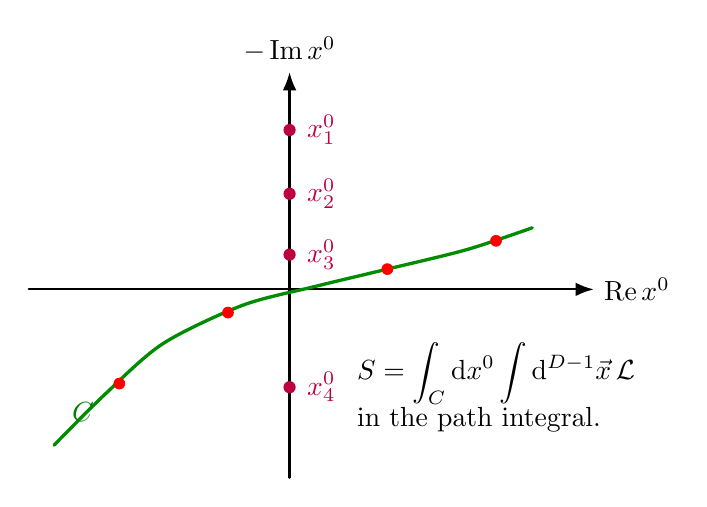
\begin{tikzpicture}[>=Latex, scale=0.92]
  \draw[->, thick] (-3.6,0) -- (4.2,0)
    node[right] {$\operatorname{Re}x^0$};
  \draw[->, thick] (0,-2.6) -- (0,3.0)
    node[above] {$-\operatorname{Im}x^0$};
  \draw[green!55!black, very thick, smooth]
    plot coordinates {
      (-3.25,-2.15) (-2.55,-1.45) (-1.75,-0.75) (-0.65,-0.22)
      (0.35,0.04) (1.35,0.28) (2.45,0.55) (3.35,0.85)
    };
  \node[green!50!black] at (-2.85,-1.7) {$C$};
  \foreach \x/\y in {-2.35/-1.30,-0.85/-0.32,1.35/0.28,2.85/0.67}
    \fill[red] (\x,\y) circle (2.3pt);
  \foreach \y/\lab in {2.20/x_1^0,1.32/x_2^0,0.48/x_3^0,-1.35/x_4^0}{
    \fill[purple] (0,\y) circle (2.4pt);
    \node[purple, right=0.10cm] at (0,\y) {$\lab$};
  }
  \node[align=left] at (2.85,-1.35)
    {$S=\displaystyle\int_C\dd x^0
      \int\dd^{D-1}\vec x\,\mathcal L$\\
     in the path integral.};
\end{tikzpicture}
\end{center}

It is most convenient to start with the Euclidean correlator
\[
  \langle\Omega|
  \hat\phi(x_1)\cdots\hat\phi(x_n)
  |\Omega\rangle
  \equiv
  \langle
  \hat\phi_E(x_1^E)\cdots\hat\phi_E(x_n^E)
  \rangle,
\]
where
\[
  x_i^0=-i\tau_i,
  \qquad
  \vec x_i=\vec x_i^E,
  \qquad
  x_i^E=(\tau_i,\vec x_i^E)\in\mathbb R^D,
  \qquad
  \hat\phi(x)=\hat\phi_E(x_E).
\]
Later we will typically omit the subscript \(E\) and write simply
\(\hat\phi\) in the context of Euclidean correlators.

The Euclidean path integral gives
\[
  \langle \phi(x_1)\cdots\phi(x_n)\rangle
  =
  \frac{1}{Z}
  \int [D\phi]\,
  e^{-S^E[\phi]}\,
  \phi(x_1)\cdots\phi(x_n),
\]
where
\[
  S^E
  =
  \int \dd^D x_E\,
  \mathcal L^E(\phi,\partial_\mu\phi),
\]
and, as in quantum mechanics,
\[
  \mathcal L^E(q,\partial_\tau q)
  =
  -\mathcal L(q,i\partial_\tau q).
\]

\begin{center}
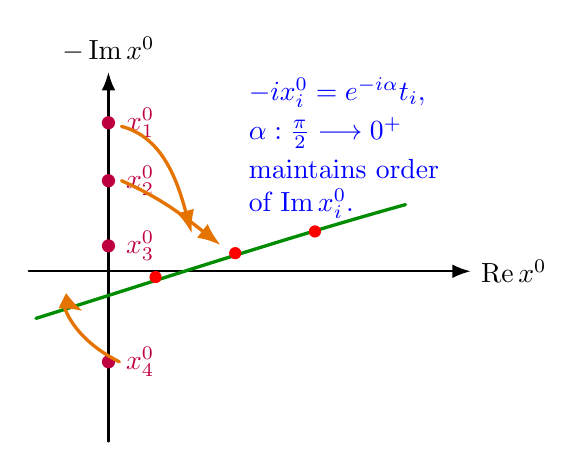
\begin{tikzpicture}[>=Latex, scale=0.92]
  \draw[->, thick] (-1.1,0) -- (5.0,0)
    node[right] {$\operatorname{Re}x^0$};
  \draw[->, thick] (0,-2.35) -- (0,2.75)
    node[above] {$-\operatorname{Im}x^0$};
  \draw[green!55!black, very thick]
    (-1.0,-0.65) .. controls (0.6,-0.15) and (2.4,0.45) .. (4.1,0.92);
  \foreach \y/\lab in {2.05/x_1^0,1.25/x_2^0,0.35/x_3^0,-1.25/x_4^0}{
    \fill[purple] (0,\y) circle (2.6pt);
    \node[purple, right=0.10cm] at (0,\y) {$\lab$};
  }
  \foreach \x/\y in {0.65/-0.08,1.75/0.25,2.85/0.55}{
    \fill[red] (\x,\y) circle (2.4pt);
  }
  \draw[->, orange!90!black, very thick]
    (0.18,2.00) .. controls (0.75,1.85) and (0.95,1.25) .. (1.15,0.52);
  \draw[->, orange!90!black, very thick]
    (0.18,1.25) .. controls (0.75,1.00) and (1.05,0.75) .. (1.55,0.36);
  \draw[->, orange!90!black, very thick]
    (0.15,-1.25) .. controls (-0.55,-0.90) and (-0.65,-0.40) .. (-0.35,-0.55);
  \node[blue, align=left] at (3.25,1.70)
    {$-i x_i^0=e^{-i\alpha}t_i,$\\[0.2em]
     $\alpha:\frac{\pi}{2}\longrightarrow 0^+$\\[0.2em]
     maintains order\\
     of \(\operatorname{Im}x_i^0\).};
\end{tikzpicture}
\end{center}

A uniform Wick rotation on all \(i=1,\ldots,n\) simultaneously leads to
\[
  \langle\Omega|
  \hat\phi(x_1)\cdots\hat\phi(x_n)
  |\Omega\rangle,
\]
and in the limit \(\alpha\to0^+\) we have a real-time correlator that is
time ordered, i.e.
\[
  x_1^0>x_2^0>\cdots>x_n^0.
\]
Conclusion: the time-ordered real-time correlator is obtained from the
Euclidean one by uniform Wick rotation on all \(x_i\)'s.

For example, in the free scalar field theory
\[
  \mathcal L
  =
  -\frac12\eta^{\mu\nu}\partial_\mu\phi\,\partial_\nu\phi
  -\frac12m^2\phi^2,
\]
the Euclidean Lagrangian is
\[
  \mathcal L^E
  =
  \frac12\sum_{\mu=1}^D(\partial_\mu\phi)^2
  +\frac12m^2\phi^2.
\]
The Euclidean two-point function is
\[
  \langle\phi(x)\phi(y)\rangle
  =
  \frac{1}{Z}
  \int [D\phi]\,
  e^{-S^E[\phi]}\,
  \phi(x)\phi(y)
  =
  G(x,y),
\]
where
\[
  (-\partial_x^2+m^2)G(x,y)=\delta^D(x-y)
\]
in Euclidean signature, and hence
\[
  G(x,y)
  =
  \int\frac{\dd^D k}{(2\pi)^D}
  \frac{e^{ik\cdot(x-y)}}{k^2+m^2}.
\]

For the continuation to real time, set
\[
  -i x^D=e^{-i\alpha}t,
  \qquad
  -i y^D=e^{-i\alpha}t',
  \qquad
  t>t',
  \qquad
  \alpha\to0^+.
\]
To maintain analyticity of \(G(x,y)\), also Wick rotate the
\(k^D\)-integration contour. Set
\[
  -ik^D=e^{+i\alpha}k^0.
\]
Then
\[
  G(x,y)
  =
  -i e^{i\alpha}
  \int
  \frac{\dd k^0\,\dd^{D-1}\vec k}{(2\pi)^D}
  \frac{
    e^{i\vec k\cdot(\vec x-\vec y)-ik^0(t-t')}
  }{
    -e^{2i\alpha}(k^0)^2+\vec k^2+m^2
  },
\]
where the overall sign comes from the orientation of the contour. The
denominator never vanishes as \(\alpha\) ranges from \(\pi/2\) to \(0^+\).

What about the \(\alpha\to0\) limit? If we set \(\alpha=0\) in the integrand,
the denominator would vanish when \(k^0\) hits
\(\pm\sqrt{\vec k^2+m^2}\), so the integral is ill-defined. To maintain
analyticity, we can add \(-i\epsilon\) to the denominator, so that its
imaginary part never vanishes, and take the \(\epsilon\to0^+\) limit after
evaluating the \(k\)-integrals.

This results in the time-ordered two-point function
\[
  \langle\Omega|
  T\hat\phi(x)\hat\phi(y)
  |\Omega\rangle
  =
  -i
  \int
  \frac{\dd k^0\,\dd^{D-1}\vec k}{(2\pi)^D}
  \frac{
    e^{i\vec k\cdot(\vec x-\vec y)-ik^0(x^0-y^0)}
  }{
    -(k^0)^2+\vec k^2+m^2-i\epsilon
  }.
\]
Equivalently,
\[
  \langle\Omega|
  T\hat\phi(x)\hat\phi(y)
  |\Omega\rangle
  =
  -i
  \int\frac{\dd^D k}{(2\pi)^D}
  \frac{e^{ik\cdot(x-y)}}{k^2+m^2-i\epsilon},
\]
where \(k^2=-(k^0)^2+\vec k^2\) is Lorentzian. The poles in the complex
\(k^0\)-plane are at
\[
  k^0
  =
  \pm\sqrt{\vec k^2+m^2-i\epsilon}.
\]

There are three useful types of Green functions in a general QFT.

The Wightman function, for
\[
  x_a=(t_a,\vec x_a)\in\mathbb R^{1,D-1},
\]
is
\[
  W(x_1,\ldots,x_n)
  =
  \langle\Omega|
  \hat\phi(x_1)\cdots\hat\phi(x_n)
  |\Omega\rangle.
\]
The time-ordered Green function is
\[
  G(x_1,\ldots,x_n)
  =
  \langle\Omega|
  T\hat\phi(x_1)\cdots\hat\phi(x_n)
  |\Omega\rangle.
\]
If \(x_{i_1}^0>x_{i_2}^0>\cdots>x_{i_n}^0\), then
\[
  G(x_1,\ldots,x_n)
  =
  \langle\Omega|
  \hat\phi(x_{i_1})\cdots\hat\phi(x_{i_n})
  |\Omega\rangle,
\]
where \((i_1,\ldots,i_n)\) is a permutation of \((1,\ldots,n)\).

The Euclidean Green function, or Schwinger function, has
\[
  x_a^E=(\tau_a,\vec x_a)\in\mathbb R^D,
\]
and is
\[
  G_E(x_1^E,\ldots,x_n^E)
  =
  W(x_{i_1},\ldots,x_{i_n})
  \Big|_{t_a\to -i\tau_a}.
\]
This is the analytic continuation for
\[
  \tau_{i_1}\ge \tau_{i_2}\ge\cdots\ge\tau_{i_n},
\]
with \((i_1,\ldots,i_n)\) a permutation of \((1,\ldots,n)\).

\section{Spectral Representations and Particle Content}

The Wightman functions are most directly related to the spectrum. For example,
\[
  \langle\Omega|\hat\phi(x)\hat\phi(y)|\Omega\rangle
  =
  \int \dd\alpha\,
  \langle\Omega|\hat\phi(x)|\alpha\rangle
  \langle\alpha|\hat\phi(y)|\Omega\rangle,
\]
where
\[
  \int \dd\alpha\,|\alpha\rangle\langle\alpha|=1,
  \qquad
  \hat P^\mu|\alpha\rangle=P_\alpha^\mu|\alpha\rangle.
\]
Using translation invariance,
\[
\begin{aligned}
  \langle\Omega|\hat\phi(x)\hat\phi(y)|\Omega\rangle
  &=
  \int \dd\alpha\,
  \langle\Omega|
  e^{i\hat P\cdot x}\hat\phi(0)e^{-i\hat P\cdot x}
  |\alpha\rangle
  \langle\alpha|
  e^{i\hat P\cdot y}\hat\phi(0)e^{-i\hat P\cdot y}
  |\Omega\rangle  \\
  &=
  \int \dd\alpha\,
  e^{iP_\alpha\cdot(x-y)}
  \left|\langle\Omega|\hat\phi(0)|\alpha\rangle\right|^2  \\
  &=
  \int \dd^D k\, e^{ik\cdot(x-y)}
  \int \dd\alpha\,\delta^D(k-P_\alpha)
  \left|\langle\Omega|\hat\phi(0)|\alpha\rangle\right|^2 .
\end{aligned}
\]
The final factor is invariant under the Lorentz transformation
\[
  k^\mu\mapsto \Lambda^\mu{}_\nu k^\nu .
\]
Indeed, Lorentz transformations act unitarily, and for a scalar field
\[
  U(\Lambda)\hat\phi(x)U(\Lambda)^{-1}
  =
  \hat\phi(\Lambda\cdot x),
\]
while
\[
  U(\Lambda)|\alpha\rangle=|\alpha'\rangle,
  \qquad
  P_{\alpha'}^\mu=\Lambda^\mu{}_\nu P_\alpha^\nu .
\]
Thus
\[
\begin{aligned}
  &\int \dd\alpha\,
  \delta^D(\Lambda k-P_\alpha)
  \left|\langle\Omega|\hat\phi(0)|\alpha\rangle\right|^2  \\
  &\qquad =
  \int \dd\alpha\,
  \delta^D(k-P_\alpha)
  \left|
    \langle\Omega|
    U(\Lambda)\hat\phi(0)U(\Lambda)^{-1}
    |\alpha\rangle
  \right|^2  \\
  &\qquad =
  \int \dd\alpha\,
  \delta^D(k-P_\alpha)
  \left|\langle\Omega|\hat\phi(0)|\alpha\rangle\right|^2 .
\end{aligned}
\]
We can therefore write
\[
  \int \dd\alpha\,
  \delta^D(k-P_\alpha)
  \left|\langle\Omega|\hat\phi(0)|\alpha\rangle\right|^2
  =
  \frac{\theta(k^0)}{(2\pi)^{D-1}}\rho(-k^2),
\]
where \(k^2=-(k^0)^2+\vec k^2\). The function
\(\rho(-k^2)\) is non-negative. The appearance of \(\theta(k^0)\),
where
\[
  \theta(k^0)=
  \begin{cases}
    1, & k^0\ge 0,\\
    0, & k^0<0,
  \end{cases}
\]
is due to the assumption that \(P^0\ge 0\) for all physical states.
It follows that
\[
  \langle\Omega|\hat\phi(x)\hat\phi(y)|\Omega\rangle
  =
  \int \dd^D k\,
  e^{ik\cdot(x-y)}
  \frac{\theta(k^0)}{(2\pi)^{D-1}}\rho(-k^2),
\]
or equivalently
\[
  \langle\Omega|\hat\phi(x)\hat\phi(y)|\Omega\rangle
  =
  \int_0^\infty \dd\mu^2\,
  \rho(\mu^2)\Delta_+(x-y;\mu^2),
\]
where
\[
\begin{aligned}
  \Delta_+(x;\mu^2)
  &=
  \int \frac{\dd^D k}{(2\pi)^{D-1}}\,
  \theta(k^0)\delta(k^2+\mu^2)e^{ik\cdot x}  \\
  &=
  \int \frac{\dd^{D-1}\vec k}{(2\pi)^{D-1}}\,
  \frac{
    e^{i\vec k\cdot\vec x-i\sqrt{\vec k^2+\mu^2}\,x^0}
  }{2\sqrt{\vec k^2+\mu^2}} .
\end{aligned}
\]
We have already seen that
\[
  \Delta_+(x;\mu^2)=\Delta_+(-x;\mu^2)
\]
for spacelike \(x^\mu\), namely for \(x^2>0\). This is not true in
general for timelike \(x^\mu\), where \(x^2<0\).

The time-ordered Green function will be closely related to the scattering
amplitude of particles through LSZ reduction. For now,
\[
  G(x,y):=
  \langle\Omega|T\hat\phi(x)\hat\phi(y)|\Omega\rangle
\]
is
\[
\begin{aligned}
  G(x,y)
  &=
  \theta(x^0-y^0)
  \langle\Omega|\hat\phi(x)\hat\phi(y)|\Omega\rangle
  +
  \theta(y^0-x^0)
  \langle\Omega|\hat\phi(y)\hat\phi(x)|\Omega\rangle  \\
  &=
  \int_0^\infty \dd\mu^2\,\rho(\mu^2)
  \Bigl[
    \theta(x^0-y^0)\Delta_+(x-y;\mu^2)
    +
    \theta(y^0-x^0)\Delta_+(y-x;\mu^2)
  \Bigr]  \\
  &=
  \int_0^\infty \dd\mu^2\,\rho(\mu^2)
  \Delta_F(x-y;\mu^2).
\end{aligned}
\]
Here the Feynman propagator is
\[
  \Delta_F(x;\mu^2)
  =
  \int \frac{\dd^D k}{(2\pi)^D}
  \frac{-i\,e^{ik\cdot x}}{k^2+\mu^2-i\epsilon},
\]
and equivalently
\[
\begin{aligned}
  \Delta_F(x;\mu^2)
  =
  \int \frac{\dd^{D-1}\vec k}{(2\pi)^{D-1}}\,
  \frac{1}{2\sqrt{\vec k^2+\mu^2}}
  \Bigl[
    &\theta(x^0)
    e^{i\vec k\cdot\vec x-i\sqrt{\vec k^2+\mu^2}\,x^0}  \\
    &+
    \theta(-x^0)
    e^{-i\vec k\cdot\vec x+i\sqrt{\vec k^2+\mu^2}\,x^0}
  \Bigr].
\end{aligned}
\]

To see the \(i\epsilon\) prescription explicitly, consider
\[
  \int \frac{\dd k^0}{2\pi i}\,
  \frac{e^{-ik^0x^0}}{-(k^0)^2+\vec k^2+\mu^2-i\epsilon}
\]
as a contour integral on the complex \(k^0\)-plane. The poles lie at
\[
  k^0=
  \pm\sqrt{\vec k^2+\mu^2-i\epsilon}
  \simeq
  \pm\sqrt{\vec k^2+\mu^2}
  \left(1-\frac{i\epsilon}{2(\vec k^2+\mu^2)}\right).
\]

\begin{center}
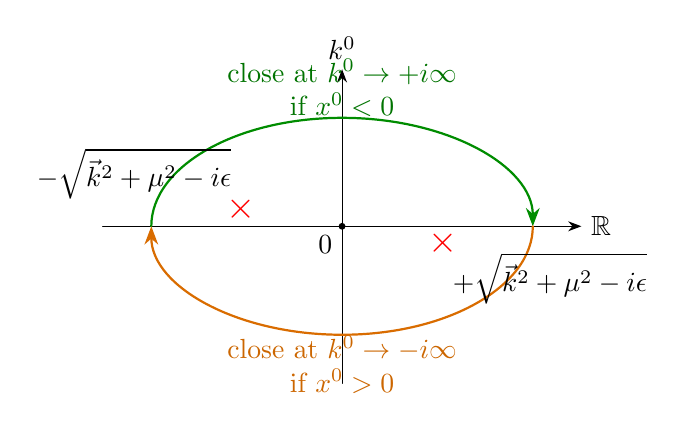
\begin{tikzpicture}[scale=0.95, >=Stealth]
  \draw[->] (-3.2,0) -- (3.2,0) node[right] {$\mathbb R$};
  \draw[->] (0,-2.1) -- (0,2.1) node[above] {$k^0$};
  \fill (0,0) circle (1.3pt) node[below left] {$0$};

  \draw[green!55!black, thick, ->]
    (-2.55,0) arc[start angle=180,end angle=0,x radius=2.55,y radius=1.45];
  \draw[orange!85!black, thick, ->]
    (2.55,0) arc[start angle=0,end angle=-180,x radius=2.55,y radius=1.45];

  \node[red, scale=1.35] at (1.35,-0.23) {$\times$};
  \node[red, scale=1.35] at (-1.35,0.23) {$\times$};
  \node[below right] at (1.35,-0.23)
    {$+\sqrt{\vec k^2+\mu^2-i\epsilon}$};
  \node[above left] at (-1.35,0.23)
    {$-\sqrt{\vec k^2+\mu^2-i\epsilon}$};

  \node[green!45!black, align=center] at (0,1.85)
    {close at \(k^0\to+i\infty\)\\if \(x^0<0\)};
  \node[orange!80!black, align=center] at (0,-1.85)
    {close at \(k^0\to-i\infty\)\\if \(x^0>0\)};
\end{tikzpicture}
\end{center}

The contour gives
\[
\begin{aligned}
  &\int \frac{\dd k^0}{2\pi i}\,
  \frac{e^{-ik^0x^0}}{-(k^0)^2+\vec k^2+\mu^2-i\epsilon}  \\
  &\quad =
  -\theta(x^0)
  \operatorname*{Res}_{k^0\to+\sqrt{\vec k^2+\mu^2-i\epsilon}}
  \frac{e^{-ik^0x^0}}{k^2+\mu^2-i\epsilon}
  +
  \theta(-x^0)
  \operatorname*{Res}_{k^0\to-\sqrt{\vec k^2+\mu^2-i\epsilon}}
  \frac{e^{-ik^0x^0}}{k^2+\mu^2-i\epsilon}  \\
  &\quad =
  -\theta(x^0)
  \left(
    \frac{e^{-i\sqrt{\vec k^2+\mu^2}\,x^0}}
         {-2\sqrt{\vec k^2+\mu^2}}
  \right)
  +
  \theta(-x^0)
  \left(
    \frac{e^{i\sqrt{\vec k^2+\mu^2}\,x^0}}
         {2\sqrt{\vec k^2+\mu^2}}
  \right).
\end{aligned}
\]
Comparing with the definition of \(\Delta_F\) above, we can write
equivalently
\[
  \Delta_F(x;\mu^2)
  =
  -i\int\frac{\dd^Dk}{(2\pi)^D}
  \frac{e^{ik\cdot x}}{k^2+\mu^2-i\epsilon}.
\]
This is the Feynman propagator.

Next consider the Euclidean Green function. The Wightman function may be
written
\[
\begin{aligned}
  W(x,y)
  &:=
  \langle\Omega|\hat\phi(x)\hat\phi(y)|\Omega\rangle  \\
  &=
  \int \dd\alpha\,
  e^{iP_\alpha\cdot(x-y)}
  \left|\langle\Omega|\hat\phi(0)|\alpha\rangle\right|^2  \\
  &\sim
  e^{i\vec P_\alpha\cdot(\vec x-\vec y)
    -iP_\alpha^0(x^0-y^0)} .
\end{aligned}
\]
Since \(P_\alpha^0\ge 0\), \(W(x,y)\) is an analytic function of complex
\(x^0\) and \(y^0\) provided
\[
  e^{-iP_\alpha^0(x^0-y^0)}
\]
is exponentially suppressed at large \(P_\alpha^0\), namely provided
\[
  \operatorname{Im}(x^0-y^0)<0.
\]
It is possible to maintain this condition while going from real
\(x^0,y^0\) to
\[
  x^0=-i\tau_1,
  \qquad
  y^0=-i\tau_2,
  \qquad
  \tau_1>\tau_2.
\]
Writing \(x_E=(\tau_1,\vec x)\) and \(y_E=(\tau_2,\vec y)\), define
\[
\begin{aligned}
  G_E(x_E,y_E)
  &:=
  \text{analytic continuation of }W(x,y)  \\
  &\qquad
  \text{to }x^0=-i\tau_1,\quad y^0=-i\tau_2
  \quad\text{for }\tau_1>\tau_2 .
\end{aligned}
\]
For \(\tau_1<\tau_2\), \(G_E(x_E,y_E)\) is instead the analytic continuation
of \(W(y,x)\). The result is
\[
  G_E(x_E,y_E)
  =
  \int_0^\infty \dd\mu^2\,\rho(\mu^2)
  \Delta_E(x_E-y_E;\mu^2),
\]
where
\[
  \Delta_E(x_E;\mu^2)
  =
  \int \frac{\dd^D k_E}{(2\pi)^D}
  \frac{e^{ik_E\cdot x_E}}{(k_E)^2+\mu^2},
  \qquad
  k_E\cdot x_E=\sum_j k_jx_j.
\]
The Euclidean Green function has the simplest analytic structure: it is
singular only when points collide, and is easiest to evaluate, for example
with numerical approximations.

\subsection*{More on the Structure of Green Functions}

The Wightman function is
\[
  \langle\Omega|\hat\phi(x)\hat\phi(y)|\Omega\rangle
  =
  \int_0^\infty \dd\mu^2\,\rho(\mu^2)\Delta_+(x-y;\mu^2),
\]
where
\[
  \rho(\mu^2)
  =
  (2\pi)^{D-1}
  \int\dd\alpha\,\delta^D(k-P_\alpha)
  \left|\langle\Omega|\hat\phi(0)|\alpha\rangle\right|^2,
  \qquad
  k^2=-\mu^2,\quad k^0>0.
\]
What is the content of \(\hat\phi(x)|\Omega\rangle\)?

\begin{center}
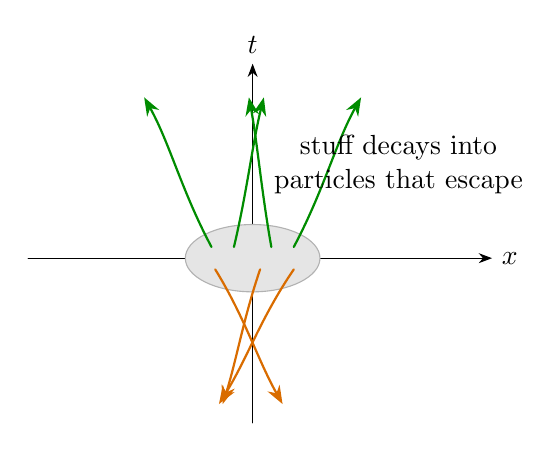
\begin{tikzpicture}[scale=0.95, >=Stealth]
  \draw[->] (-3,0) -- (3.2,0) node[right] {$x$};
  \draw[->] (0,-2.2) -- (0,2.6) node[above] {$t$};

  \fill[gray!20, draw=gray!60] (0,0) ellipse (0.9 and 0.45);
  \foreach \x/\bend in {-0.55/-18,-0.25/8,0.25/-6,0.55/18} {
    \draw[green!55!black, thick, ->]
      (\x,0.15) .. controls ({\x+\bend/45},0.9) and ({\x+\bend/32},1.55) ..
      ({\x+\bend/20},2.15);
  }
  \foreach \x/\bend in {-0.5/18,0.1/-10,0.55/-20} {
    \draw[orange!85!black, thick, ->]
      (\x,-0.15) .. controls ({\x+\bend/45},-0.8) and ({\x+\bend/32},-1.35) ..
      ({\x+\bend/20},-1.95);
  }
  \node[align=center] at (1.95,1.25)
    {stuff decays into\\particles that escape};
\end{tikzpicture}
\end{center}

At a given instance of time, a physical state may not admit any obvious
particle interpretation, but it is expected to evolve into a superposition of
states that consist of far-separated wave packets of individual particles as
\(t\to+\infty\) or \(t\to-\infty\). An underlying assumption is that
``particles'' are weakly interacting at long distance. The particles could be
strongly interacting at finite distances, but the invariant mass squared,
namely \(-P_\mu P^\mu\), of any state is identical to that of its decay
product.

Suppose there is only one species of particle, with mass \(m\). The possible
invariant masses of \(|\alpha\rangle\) are
\[
\begin{array}{rcl}
  |\Omega\rangle
  &:&
  -P^2=0, \\[2mm]
  \text{one-particle state}
  &:&
  -P^2=m^2, \\[2mm]
  \text{states that decay into two or more particles}
  &:&
  -P^2\ge (2m)^2,
\end{array}
\]
with a continuum of possible values in the multi-particle case.

Without loss of generality, we can shift \(\hat\phi(x)\) by a constant so that
\[
  \langle\Omega|\hat\phi(x)|\Omega\rangle=0.
\]
Then
\[
  \hat\phi(x)|\Omega\rangle
  =
  |\text{one-particle}\rangle
  +
  |\text{multi-particle stuff}\rangle,
\]
where the one-particle contribution has \(-P^2=m^2\), while the
multi-particle contribution has \(-P^2\ge(2m)^2\).

Assuming no internal, or spin, degree of freedom, a basis of one-particle
states is labeled by the spatial momentum \(|\vec k\rangle\), with
\[
  \hat P^i|\vec k\rangle=k^i|\vec k\rangle,
  \qquad
  i=1,\ldots,D-1,
\]
and
\[
  \hat P^0|\vec k\rangle
  =
  \sqrt{\vec k^2+m^2}\,|\vec k\rangle.
\]
Choose the normalization
\[
  \langle\vec k'|\vec k\rangle
  =
  \delta^{D-1}(\vec k'-\vec k).
\]
How does Lorentz symmetry \(U(\Lambda)\) act on \(|\vec k\rangle\)?
We expect
\[
  U(\Lambda)|\vec k\rangle
  =
  C(\Lambda,\vec k)|\Lambda\vec k\rangle,
\]
where \(\Lambda\vec k\) means the spatial component of
\((\Lambda k)^\mu=\Lambda^\mu{}_\nu k^\nu\).

Pick a reference momentum \(k_R^\mu\), with
\[
  k_R^2=k_R^\mu k_{R\mu}=-m^2.
\]
For every possible momentum \(k^\mu\), choose a standard boost
\(L^\mu{}_\nu(\vec k)\) such that
\[
  k^\mu=L^\mu{}_\nu(\vec k)k_R^\nu .
\]

\begin{center}
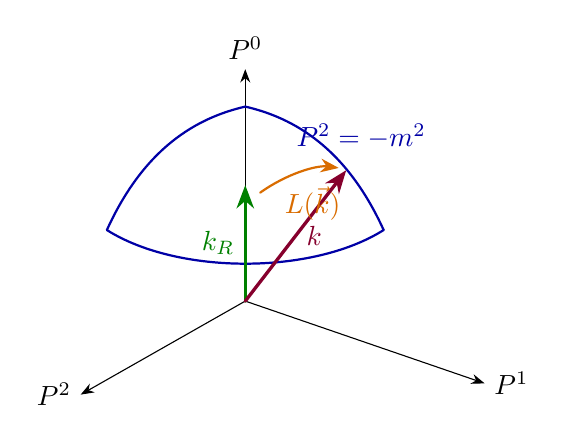
\begin{tikzpicture}[scale=0.95, >=Stealth]
  \draw[->] (0,0) -- (0,3.1) node[above] {$P^0$};
  \draw[->] (0,0) -- (3.2,-1.1) node[right] {$P^1$};
  \draw[->] (0,0) -- (-2.2,-1.25) node[left] {$P^2$};

  \draw[blue!65!black, thick]
    (-1.85,0.95) .. controls (-0.9,0.35) and (0.9,0.35) .. (1.85,0.95);
  \draw[blue!65!black, thick]
    (-1.85,0.95) .. controls (-1.35,2.05) and (-0.65,2.45) .. (0,2.6);
  \draw[blue!65!black, thick]
    (1.85,0.95) .. controls (1.35,2.05) and (0.65,2.45) .. (0,2.6);
  \node[blue!65!black] at (1.55,2.2) {$P^2=-m^2$};

  \draw[green!50!black, very thick, ->] (0,0) -- (0,1.55)
    node[midway,left] {$k_R$};
  \draw[purple!70!black, very thick, ->] (0,0) -- (1.35,1.75)
    node[midway,right] {$k$};
  \draw[orange!85!black, thick, ->]
    (0.2,1.45) .. controls (0.55,1.7) and (0.95,1.82) .. (1.25,1.78);
  \node[orange!85!black] at (0.9,1.3) {$L(\vec k)$};
\end{tikzpicture}
\end{center}

We can specify the phase of \(|\vec k\rangle\) by defining
\[
  |\vec k\rangle
  :=
  N(\vec k)U(L(\vec k))|\vec k_R\rangle,
\]
where \(N(\vec k)\) is a normalization factor to be determined. For any
Lorentz transformation \(\Lambda\),
\[
\begin{aligned}
  U(\Lambda)|\vec k\rangle
  &=
  N(\vec k)U(\Lambda)U(L(\vec k))|\vec k_R\rangle  \\
  &=
  N(\vec k)U(\Lambda L(\vec k))|\vec k_R\rangle  \\
  &=
  N(\vec k)
  U(L(\Lambda\vec k))
  U(L(\Lambda\vec k)^{-1}\Lambda L(\vec k))
  |\vec k_R\rangle .
\end{aligned}
\]
Let
\[
  W=L(\Lambda\vec k)^{-1}\Lambda L(\vec k).
\]
Then \(W\) fixes \(k_R\):
\[
  Wk_R
  =
  L(\Lambda\vec k)^{-1}\Lambda L(\vec k)k_R
  =
  L(\Lambda\vec k)^{-1}\Lambda k
  =
  k_R.
\]
Thus \(U(W)|\vec k_R\rangle\) is proportional to \(|\vec k_R\rangle\);
\(U(W)\) acts on \(|\vec k_R\rangle\) by multiplication by a phase
\(D(W)\). Therefore
\[
\begin{aligned}
  U(\Lambda)|\vec k\rangle
  &=
  N(\vec k)U(L(\Lambda\vec k))D(W)|\vec k_R\rangle  \\
  &=
  \frac{N(\vec k)}{N(\Lambda\vec k)}
  D(W)|\Lambda\vec k\rangle .
\end{aligned}
\]
This is \(C(\Lambda,\vec k)\).

For now assume \(m>0\). Without loss of generality, choose
\[
  k_R^\mu=(m,\vec 0).
\]
Then \(W\) is a Lorentz transformation that fixes \(k_R\), i.e. a spatial
rotation, \(W\in \operatorname{SO}(D-1)\). Moreover
\[
  D(W_1W_2)=D(W_1)D(W_2),
  \qquad
  |D(W)|=1.
\]
For \(D=4\), \(\operatorname{SO}(D-1)\) is non-abelian. Furthermore every
element of \(\operatorname{SO}(D-1)\) can be written as a commutator
\[
  W=XYX^{-1}Y^{-1},
  \qquad
  X,Y\in\operatorname{SO}(D-1).
\]
Therefore
\[
  D(W)=D(X)D(Y)D(X)^{-1}D(Y)^{-1}=1.
\]
Such particles are called scalar particles; this has no obvious relation to
the phrase scalar fields.

We conclude that
\[
  U(\Lambda)|\vec k\rangle
  =
  \frac{N(\vec k)}{N(\Lambda\vec k)}|\Lambda\vec k\rangle.
\]
Compare
\[
\begin{aligned}
  \langle\vec k'|U(\Lambda)^\dagger U(\Lambda)|\vec k\rangle
  &=
  \frac{N(\vec k)N(\vec k')}
       {N(\Lambda\vec k)N(\Lambda\vec k')}
  \langle\Lambda\vec k'|\Lambda\vec k\rangle  \\
  &=
  \left(\frac{N(\vec k)}{N(\Lambda\vec k)}\right)^2
  \delta^{D-1}(\Lambda\vec k'-\Lambda\vec k),
\end{aligned}
\]
with
\[
  \langle\vec k'|\vec k\rangle
  =
  \delta^{D-1}(\vec k'-\vec k).
\]
Using
\[
  \delta^D(k'-k)
  =
  2k^0\delta(k'^2-k^2)\delta^{D-1}(\vec k'-\vec k),
\]
under \(k\to\Lambda k\) and \(k'\to\Lambda k'\), we obtain
\[
  \delta^{D-1}(\vec k'-\vec k)
  =
  \frac{(\Lambda k)^0}{k^0}
  \delta^{D-1}(\Lambda\vec k'-\Lambda\vec k).
\]
Since \(N(\vec k_R)=1\), this gives
\[
  N(\vec k)=\sqrt{\frac{m}{k^0}}.
\]

Returning to
\[
  \hat\phi(x)|\Omega\rangle
  =
  |\text{one-particle}\rangle
  +
  |\text{multi-particle}\rangle,
\]
let us study the overlap with one-particle states:
\[
\begin{aligned}
  \langle\vec k|\hat\phi(x)|\Omega\rangle
  &=
  \langle\vec k|
  e^{-i\hat P\cdot x}\hat\phi(0)e^{i\hat P\cdot x}
  |\Omega\rangle  \\
  &=
  e^{ik\cdot x}
  \langle\vec k|\hat\phi(0)|\Omega\rangle .
\end{aligned}
\]
Lorentz invariance implies
\[
\begin{aligned}
  \langle\vec k|\hat\phi(0)|\Omega\rangle
  &=
  \langle\vec k|U(\Lambda)^{-1}\hat\phi(0)U(\Lambda)|\Omega\rangle  \\
  &=
  \frac{N(\Lambda\vec k)}{N(\vec k)}
  \langle\Lambda\vec k|\hat\phi(0)|\Omega\rangle,
\end{aligned}
\]
and hence
\[
  \langle\vec k|\hat\phi(0)|\Omega\rangle
  \propto
  N(\vec k)
  =
  \sqrt{\frac{m}{k^0}}.
\]
We can write
\[
  \langle\vec k|\hat\phi(0)|\Omega\rangle
  =
  \left[
    \frac{Z}{(2\pi)^{D-1}2\omega_{\vec k}}
  \right]^{1/2},
  \qquad
  \omega_{\vec k}=\sqrt{\vec k^2+m^2},
\]
where \(Z\ge 0\) is a constant. The constant \(Z\) is often called the
field renormalization constant. For a free scalar field, \(Z=1\). It is
sometimes asserted that \(Z\) is unphysical; this is false. The constant \(Z\)
is intrinsic to the field operator \(\hat\phi(x)\), and is unambiguously
defined if \(\hat\phi(x)\) is defined.

Recall the spectral function
\[
  \rho(\mu^2)
  =
  (2\pi)^{D-1}
  \int\dd\alpha\,
  \delta^D(p-P_\alpha)
  \left|\langle\alpha|\hat\phi(0)|\Omega\rangle\right|^2,
  \qquad
  p^2=-\mu^2,\quad p^0>0.
\]
The one-particle contribution gives
\[
\begin{aligned}
  \rho(\mu^2)
  &=
  \int\dd^{D-1}\vec k\,
  \delta^D(p-k)
  \frac{Z}{2\omega_{\vec k}}
  +
  \text{multi-particle }|\alpha\rangle\text{ contributions}  \\
  &=
  Z\delta(\mu^2-m^2)+\sigma(\mu^2).
\end{aligned}
\]

\begin{center}
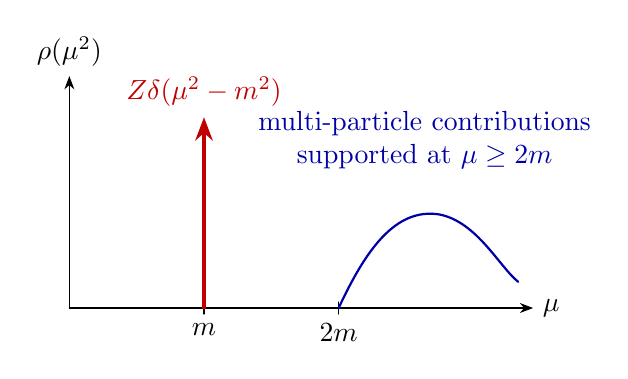
\begin{tikzpicture}[scale=0.95, >=Stealth]
  \draw[->] (0,0) -- (6.2,0) node[right] {$\mu$};
  \draw[->] (0,0) -- (0,3.1) node[above] {$\rho(\mu^2)$};
  \draw (1.8,0.08) -- (1.8,-0.08) node[below] {$m$};
  \draw (3.6,0.08) -- (3.6,-0.08) node[below] {$2m$};

  \draw[red!75!black, very thick, ->] (1.8,0) -- (1.8,2.55)
    node[above] {$Z\delta(\mu^2-m^2)$};
  \draw[blue!65!black, thick]
    (3.6,0) .. controls (3.95,0.75) and (4.35,1.35) .. (4.95,1.25)
    .. controls (5.45,1.15) and (5.75,0.55) .. (6.0,0.35);
  \node[blue!65!black, align=center] at (4.75,2.25)
    {multi-particle contributions\\supported at \(\mu\ge 2m\)};
\end{tikzpicture}
\end{center}

Thus
\[
  \rho(\mu^2)
  =
  Z\delta(\mu^2-m^2)+\sigma(\mu^2),
\]
where the multi-particle contribution is supported at invariant mass
\(\mu\ge 2m\). It follows that
\[
  \langle\Omega|T\hat\phi(x)\hat\phi(y)|\Omega\rangle
  =
  Z\Delta_F(x-y;m^2)
  +
  \int_{4m^2}^{\infty}\dd\mu^2\,
  \sigma(\mu^2)\Delta_F(x-y;\mu^2).
\]
This is the Kallen-Lehmann spectral representation.

\section{Computation of Correlation Functions in Perturbation Theory}

We illustrate the computation of correlation functions in perturbation theory
with scalar \(\phi^4\) theory. In Lorentzian signature,
\[
  \mathcal L
  =
  -\frac12\eta^{\mu\nu}\partial_\mu\phi\,\partial_\nu\phi
  -\frac12m^2\phi^2
  -\frac{1}{4!}g\phi^4 .
\]
In Euclidean signature,
\[
  \mathcal L^E
  =
  \frac12(\partial_\mu\phi)^2
  +\frac12m^2\phi^2
  +\frac{1}{4!}g\phi^4 .
\]
The Euclidean correlation functions are
\[
\begin{aligned}
  \langle\phi(x_1^E)\cdots\phi(x_n^E)\rangle
  &=
  \frac{
    \int[D\phi]\,
    e^{-S^E[\phi]}\,
    \phi(x_1^E)\cdots\phi(x_n^E)
  }{
    \int[D\phi]\,e^{-S^E[\phi]}
  }  \\
  &=
  \sum
  \text{graphs whose connected components are connected to external }
  \phi\text{-lines}.
\end{aligned}
\]

\begin{center}
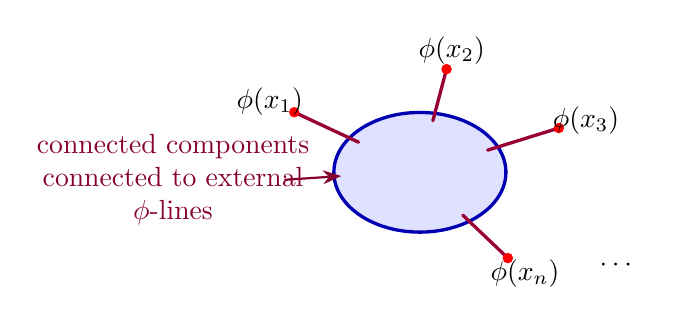
\begin{tikzpicture}[scale=0.95, >=Stealth]
  \fill[blue!12, draw=blue!70!black, very thick] (0,0) ellipse (1.15 and 0.8);
  \foreach \ang/\lab in {145/{\phi(x_1)},80/{\phi(x_2)},25/{\phi(x_3)},-55/{\phi(x_n)}} {
    \draw[purple!80!black, very thick]
      ({1.0*cos(\ang)},{0.7*sin(\ang)}) --
      ({2.05*cos(\ang)},{1.4*sin(\ang)});
    \fill[red] ({2.05*cos(\ang)},{1.4*sin(\ang)}) circle (2pt);
    \node at ({2.45*cos(\ang)},{1.65*sin(\ang)}) {$\lab$};
  }
  \node[purple!70!black, align=center] at (-3.3,-0.1)
    {connected components\\connected to external\\\(\phi\)-lines};
  \draw[purple!70!black, thick, ->] (-1.8,-0.1) -- (-1.05,-0.05);
  \node at (2.65,-1.25) {$\cdots$};
\end{tikzpicture}
\end{center}

For the two-point function,
\[
  \langle\phi(x)\phi(y)\rangle
\]
has a graph expansion of the form
\[
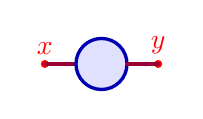
\begin{tikzpicture}[baseline=-0.45ex, scale=0.72]
  \fill[red] (-1,0) circle (2pt) node[above] {$x$};
  \fill[red] (1,0) circle (2pt) node[above] {$y$};
  \draw[purple!80!black, very thick] (-1,0)--(-0.45,0);
  \fill[blue!12, draw=blue!70!black, very thick] (0,0) circle (0.45);
  \draw[purple!80!black, very thick] (0.45,0)--(1,0);
\end{tikzpicture}
\quad=\quad
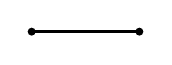
\begin{tikzpicture}[baseline=-0.45ex, scale=0.72]
  \fill ( -0.95,0) circle (2pt);
  \fill ( 0.95,0) circle (2pt);
  \draw[very thick] (-0.95,0)--(0.95,0);
\end{tikzpicture}
\quad+\quad
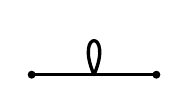
\begin{tikzpicture}[baseline=-0.45ex, scale=0.72]
  \fill (-1.1,0) circle (2pt);
  \fill (1.1,0) circle (2pt);
  \draw[very thick] (-1.1,0)--(1.1,0);
  \draw[very thick] (0,0) .. controls (-0.35,0.8) and (0.35,0.8) .. (0,0);
\end{tikzpicture}
\quad+\quad
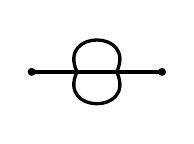
\begin{tikzpicture}[baseline=-0.45ex, scale=0.72]
  \fill (-1.15,0) circle (2pt);
  \fill (1.15,0) circle (2pt);
  \draw[very thick] (-1.15,0)--(1.15,0);
  \draw[very thick] (-0.35,0) .. controls (-0.7,0.75) and (0.7,0.75) .. (0.35,0);
  \draw[very thick] (-0.35,0) .. controls (-0.7,-0.75) and (0.7,-0.75) .. (0.35,0);
\end{tikzpicture}
\quad+\quad
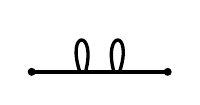
\begin{tikzpicture}[baseline=-0.45ex, scale=0.72]
  \fill (-1.2,0) circle (2pt);
  \fill (1.2,0) circle (2pt);
  \draw[very thick] (-1.2,0)--(1.2,0);
  \draw[very thick] (-0.35,0) .. controls (-0.6,0.75) and (-0.05,0.75) .. (-0.25,0);
  \draw[very thick] (0.35,0) .. controls (0.6,0.75) and (0.05,0.75) .. (0.25,0);
\end{tikzpicture}
\quad+\cdots .
\]
Writing
\[
  G_E(x,y)
  =
  \int\frac{\dd^D k}{(2\pi)^D}
  e^{ik\cdot(x-y)}\widetilde G_E(k),
\]
the Kallen-Lehmann representation says
\[
  G_E(x,y)
  =
  \int_0^\infty\dd\mu^2\,\rho(\mu^2)
  \int\frac{\dd^D k}{(2\pi)^D}
  \frac{e^{ik\cdot(x-y)}}{k^2+\mu^2}.
\]
The self-energy \(\Sigma(k)\) is obtained from one-particle-irreducible
graphs after amputating the external propagators:
\[
  \widetilde G_E(k)
  =
  \frac{1}{k^2+m^2-\Sigma(k)}.
\]
Diagrammatically,
\[
\Sigma(k)
=
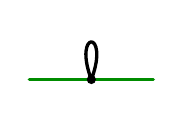
\begin{tikzpicture}[baseline=-0.45ex, scale=0.75]
  \draw[green!55!black, very thick] (-1.05,0)--(1.05,0);
  \fill (0,0) circle (2.2pt);
  \draw[very thick] (0,0) .. controls (-0.32,0.85) and (0.32,0.85) .. (0,0);
\end{tikzpicture}
\quad+\quad
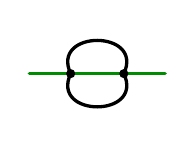
\begin{tikzpicture}[baseline=-0.45ex, scale=0.75]
  \draw[green!55!black, very thick] (-1.15,0)--(1.15,0);
  \fill (-0.45,0) circle (2.2pt);
  \fill (0.45,0) circle (2.2pt);
  \draw[very thick] (-0.45,0) .. controls (-0.8,0.75) and (0.8,0.75) .. (0.45,0);
  \draw[very thick] (-0.45,0) .. controls (-0.8,-0.75) and (0.8,-0.75) .. (0.45,0);
\end{tikzpicture}
\quad+\quad

\begin{tikzpicture}[baseline=-0.45ex, scale=0.75]
  \draw[green!55!black, very thick] (-1.2,0)--(1.2,0);
  \fill (-0.5,0) circle (2.2pt);
  \fill (0.5,0) circle (2.2pt);
  \draw[very thick] (-0.5,0) .. controls (-0.7,0.75) and (-0.1,0.75) .. (-0.4,0);
  \draw[very thick] (-0.5,0) .. controls (-0.2,0.75) and (0.2,0.75) .. (0.5,0);
  \draw[very thick] (0.5,0) .. controls (0.7,0.75) and (0.1,0.75) .. (0.4,0);
\end{tikzpicture}
\quad+\cdots .
\]

The Euclidean Feynman rules are as follows. A propagator carrying momentum
\(k\) contributes
\[
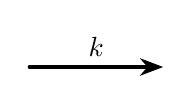
\begin{tikzpicture}[baseline=-0.45ex, scale=0.85, >=Stealth]
  \draw[very thick, ->] (-1,0)--(1,0) node[midway, above] {$k$};
\end{tikzpicture}
\qquad =\qquad
\frac{1}{k^2+m^2}.
\]
A vertex contributes
\[
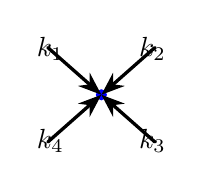
\begin{tikzpicture}[baseline=-0.45ex, scale=0.8, >=Stealth]
  \fill[blue] (0,0) circle (2.5pt);
  \draw[very thick, ->] (-0.85,0.75)--(0,0) node[midway, above left] {$k_1$};
  \draw[very thick, ->] (0.85,0.75)--(0,0) node[midway, above right] {$k_2$};
  \draw[very thick, ->] (0.85,-0.75)--(0,0) node[midway, below right] {$k_3$};
  \draw[very thick, ->] (-0.85,-0.75)--(0,0) node[midway, below left] {$k_4$};
\end{tikzpicture}
\qquad =\qquad
-\frac{g}{4!}\,(2\pi)^D
\delta^D(k_1+k_2+k_3+k_4).
\]
For example, the tadpole contribution is
\[
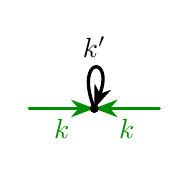
\begin{tikzpicture}[baseline=-0.45ex, scale=0.75, >=Stealth]
  \draw[green!55!black, very thick, ->] (-1.1,0)--(0,0) node[midway, below] {$k$};
  \draw[green!55!black, very thick, ->] (1.1,0)--(0,0) node[midway, below] {$k$};
  \fill (0,0) circle (2.2pt);
  \draw[very thick, ->] (0,0) .. controls (-0.35,0.9) and (0.35,0.9) .. (0,0)
    node[midway, above] {$k'$};
\end{tikzpicture}
\quad=\quad
4\cdot\frac{3!}{2}
\left(-\frac{g}{4!}\right)
\int\frac{\dd^D k'}{(2\pi)^D}\frac{1}{k'^2+m^2}
\quad=\quad
-\frac{g}{2}
\int\frac{\dd^D k'}{(2\pi)^D}\frac{1}{k'^2+m^2}.
\]
The sunset contribution is
\[
\begin{aligned}
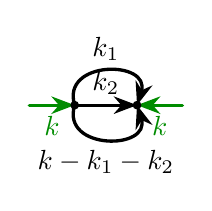
\begin{tikzpicture}[baseline=-0.45ex, scale=0.72, >=Stealth]
  \draw[green!55!black, very thick, ->] (-1.35,0)--(-0.55,0) node[midway, below] {$k$};
  \draw[green!55!black, very thick, ->] (1.35,0)--(0.55,0) node[midway, below] {$k$};
  \fill (-0.55,0) circle (2.2pt);
  \fill (0.55,0) circle (2.2pt);
  \draw[very thick, ->] (-0.55,0) .. controls (-0.8,0.8) and (0.8,0.8) .. (0.55,0)
    node[midway, above] {$k_1$};
  \draw[very thick, ->] (-0.55,0)--(0.55,0) node[midway, above] {$k_2$};
  \draw[very thick, ->] (-0.55,0) .. controls (-0.8,-0.8) and (0.8,-0.8) .. (0.55,0)
    node[midway, below] {$k-k_1-k_2$};
\end{tikzpicture}
&=
4\cdot 4!
\left(-\frac{g}{4!}\right)^2
\int\frac{\dd^D k_1\,\dd^D k_2}{(2\pi)^{2D}}\,
\frac{1}{
  (k_1^2+m^2)(k_2^2+m^2)
  ((k-k_1-k_2)^2+m^2)
}  \\
&=
\frac{g^2}{6}
\int\frac{\dd^D k_1\,\dd^D k_2}{(2\pi)^{2D}}\,
\frac{1}{
  (k_1^2+m^2)(k_2^2+m^2)
  ((k-k_1-k_2)^2+m^2)
}.
\end{aligned}
\]

Let us interpret the order \(g\) contribution to \(\Sigma(k)\),
\[
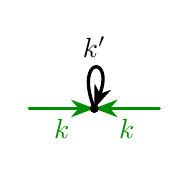
\begin{tikzpicture}[baseline=-0.45ex, scale=0.75, >=Stealth]
  \draw[green!55!black, very thick, ->] (-1.1,0)--(0,0) node[midway, below] {$k$};
  \draw[green!55!black, very thick, ->] (1.1,0)--(0,0) node[midway, below] {$k$};
  \fill (0,0) circle (2.2pt);
  \draw[very thick, ->] (0,0) .. controls (-0.35,0.9) and (0.35,0.9) .. (0,0)
    node[midway, above] {$k'$};
\end{tikzpicture}
\quad=\quad
-\frac{g}{2}
\int\frac{\dd^D k'}{(2\pi)^D}\frac{1}{k'^2+m^2}.
\]
This is divergent for \(D\ge 2\), but independent of \(k\).
First, regularize the path integral:
\[
  \int[D\phi]
  \longrightarrow
  \int \prod_{|k|\le\Lambda}\dd\widetilde\phi(k).
\]
Then
\[
\begin{aligned}
  -\frac{g}{2}
  \int_{|k'|\le\Lambda}
  \frac{\dd^D k'}{(2\pi)^D}\frac{1}{k'^2+m^2}
  &=
  -\frac{g}{2}
  \frac{\operatorname{vol}(S^{D-1})}{(2\pi)^D}
  \int_0^\Lambda \dd k\,
  \frac{k^{D-1}}{k^2+m^2}  \\
  &\equiv
  -g C_1 .
\end{aligned}
\]
Here
\[
  \operatorname{vol}(S^{D-1})
  =
  \frac{2\pi^{D/2}}{\Gamma(D/2)}
\]
is the area of the unit \((D-1)\)-sphere, and
\[
  \int_0^\Lambda \dd k\,\frac{k^{D-1}}{k^2+m^2}
  =
  \begin{cases}
    \dfrac12\log\dfrac{\Lambda^2+m^2}{m^2}, & D=2,\\[3mm]
    \dfrac{\Lambda^{D-2}}{D-2}+\cdots, & D\ge 3.
  \end{cases}
\]

Recall the Kallen-Lehmann spectral representation:
\[
  \widetilde G_E(k)
  =
  \frac{1}{k^2+m^2-\Sigma(k)}
  =
  \frac{Z}{k^2+m_*^2}
  +
  \int_{\mu^2\ge 4m_*^2}\dd\mu^2\,
  \frac{\sigma(\mu^2)}{k^2+\mu^2}.
\]
The parameter \(m_*\) is the actual mass of the particle, corresponding to
the pole in \(k^2\), or just \(k^D\) at fixed
\(\vec k=(k^1,\ldots,k^{D-1})\), closest to the origin. A constant term at
order \(g\) in \(\Sigma(k)\) shifts the pole position:
\[
  m_*^2=m^2+gC_1+O(g^2),
\]
where
\[
  C_1\sim
  \begin{cases}
    \log\Lambda, & D=2,\\
    \Lambda^{D-2}, & D\ge 3.
  \end{cases}
\]

The interpretation is as follows.
\begin{enumerate}[label=\arabic*.]
  \item \(m_*\) is the mass of the particle.
  \item \(m\) is just some parameter in the Lagrangian; its relation to the
  physical mass is dependent on the regularization scheme.
  \item It is standard terminology to refer to \(m\) as the bare mass, and to
  the Lagrangian that enters the regularized path integral as the bare
  Lagrangian.
  \item One might be slightly disturbed by the fact that while the difference
  between \(m^2\) and \(m_*^2\) is formally suppressed by the coupling \(g\),
  the coefficient \(C_1\) diverges as \(\Lambda\to\infty\), and so \(gC_1\)
  is not exactly small.
\end{enumerate}

One way to handle this in a consistent manner in perturbation theory is to
write
\[
  m^2=m_R^2+\delta m^2,
\]
where \(m_R\) is a finite renormalized mass close to \(m_*\), and
\(\delta m^2\) is viewed as a counterterm, diverging as
\(\Lambda\to\infty\), but appearing at order \(g\). Generally,
\[
  \delta m^2=\sum_{n=1}^{\infty}(\delta m^2)^{(n)}g^n .
\]
The coefficient \((\delta m^2)^{(n)}\) is chosen to cancel the divergent
contribution to the pole position \(m_*^2\) at order \(g^n\) in perturbation
theory. For example,
\[
  m_*^2=m_R^2+\delta m^2+gC_1+O(g^2),
\]
so we choose
\[
  (\delta m^2)^{(1)}=-C_1+\text{finite}.
\]
Correspondingly, we split the bare Lagrangian as
\[
  \mathcal L^E
  =
  \mathcal L_R^E+\Delta\mathcal L^E,
  \qquad
  \Delta\mathcal L^E=\frac12\delta m^2\phi^2,
\]
where \(\mathcal L_R^E\) contains the term \(\frac12m_R^2\phi^2\). We then
treat \(\Delta\mathcal L^E\) as producing interaction vertices at order
\(g^n\):
\[

\begin{tikzpicture}[baseline=-0.45ex, scale=0.85]
  \draw[purple!80!black, very thick] (-1,0)--(1,0);
  \fill (0,0) circle (2.4pt);
\end{tikzpicture}
\qquad\longleftrightarrow\qquad
-(\delta m^2)^{(n)}g^n\phi^2 .
\]
The separation of \(m^2\) into \(m_R^2\) and \(\delta m^2\) is entirely ad hoc.
Its only purpose is to reorganize perturbation theory so that when we take
\(\Lambda\to\infty\), divergences cancel manifestly at each order in \(g\), as
opposed to cancelling divergences between different orders in \(g\), for
example between \(m^2\) at zeroth order and \(C_1g\) at first order.

To make meaningful physical predictions, we should pick a regularization
scheme, find the relation between \(m\) and \(m_*\), compute observables using
the Lagrangian that includes \(m^2=m_R^2+\delta m^2\), and express the result
in terms of \(m_*\), the physical mass.

For a four-point function,
\[
  \langle
    \phi(x_1^E)\phi(x_2^E)\phi(x_3^E)\phi(x_4^E)
  \rangle,
\]
the disconnected and connected pieces are
\[
\begin{aligned}
  &\langle
    \phi(x_1^E)\phi(x_2^E)\phi(x_3^E)\phi(x_4^E)
  \rangle  \\
  &\quad =
  \langle\phi(x_1^E)\phi(x_2^E)\rangle
  \langle\phi(x_3^E)\phi(x_4^E)\rangle
  +(2\leftrightarrow 4)
  +(2\leftrightarrow 3)  \\
  &\qquad
  +
  \langle
    \phi(x_1^E)\phi(x_2^E)\phi(x_3^E)\phi(x_4^E)
  \rangle_{\mathrm{conn}} .
\end{aligned}
\]

\begin{center}
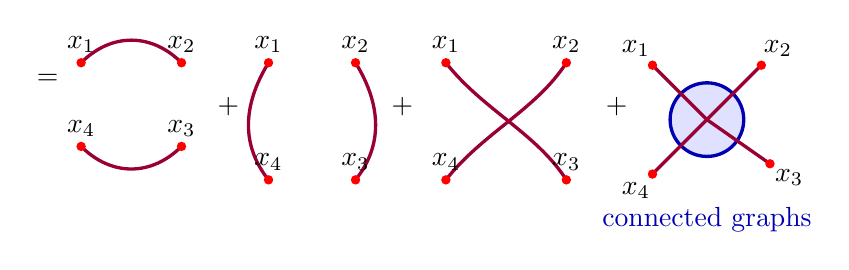
\begin{tikzpicture}[scale=0.85]
  \node at (-0.5,1.65) {$=$};
  \draw[purple!80!black, very thick] (0,1.9) .. controls (0.45,2.35) and (1.05,2.35) .. (1.5,1.9);
  \draw[purple!80!black, very thick] (0,0.65) .. controls (0.45,0.2) and (1.05,0.2) .. (1.5,0.65);
  \foreach \p/\lab in {(0,1.9)/x_1,(1.5,1.9)/x_2,(1.5,0.65)/x_3,(0,0.65)/x_4} {
    \fill[red] \p circle (2pt);
    \node[above] at \p {$\lab$};
  }

  \node at (2.2,1.25) {$+$};
  \draw[purple!80!black, very thick] (2.8,1.9) .. controls (2.4,1.25) and (2.4,0.65) .. (2.8,0.15);
  \draw[purple!80!black, very thick] (4.1,1.9) .. controls (4.5,1.25) and (4.5,0.65) .. (4.1,0.15);
  \foreach \p/\lab in {(2.8,1.9)/x_1,(4.1,1.9)/x_2,(4.1,0.15)/x_3,(2.8,0.15)/x_4} {
    \fill[red] \p circle (2pt);
    \node[above] at \p {$\lab$};
  }

  \node at (4.8,1.25) {$+$};
  \draw[purple!80!black, very thick] (5.45,1.9) .. controls (6.0,1.2) and (6.8,0.85) .. (7.25,0.15);
  \draw[purple!80!black, very thick] (7.25,1.9) .. controls (6.8,1.2) and (6.0,0.85) .. (5.45,0.15);
  \foreach \p/\lab in {(5.45,1.9)/x_1,(7.25,1.9)/x_2,(7.25,0.15)/x_3,(5.45,0.15)/x_4} {
    \fill[red] \p circle (2pt);
    \node[above] at \p {$\lab$};
  }

  \node at (8.0,1.25) {$+$};
  \fill[blue!12, draw=blue!70!black, very thick] (9.35,1.05) circle (0.55);
  \foreach \ang/\lab in {135/x_1,45/x_2,-35/x_3,-135/x_4} {
    \draw[purple!80!black, very thick]
      (9.35,1.05) -- ({9.35+1.15*cos(\ang)},{1.05+1.15*sin(\ang)});
    \fill[red] ({9.35+1.15*cos(\ang)},{1.05+1.15*sin(\ang)}) circle (2pt);
    \node at ({9.35+1.5*cos(\ang)},{1.05+1.5*sin(\ang)}) {$\lab$};
  }
  \node[blue!70!black] at (9.35,-0.45) {connected graphs};
\end{tikzpicture}
\end{center}

The final term is the connected correlator.

Define its Fourier transform by
\[
\begin{aligned}
  G_E^{\mathrm{conn}}(x_1^E,\ldots,x_4^E)
  &=
  \left\langle
    \phi(x_1^E)\cdots\phi(x_4^E)
  \right\rangle_{\mathrm{conn}}  \\
  &\equiv
  \int
  \frac{\dd^Dk_1^E}{(2\pi)^D}\cdots
  \frac{\dd^Dk_4^E}{(2\pi)^D}\,
  \ee^{\ii k_1^E\cdot x_1^E+\cdots+\ii k_4^E\cdot x_4^E}
  \widetilde G_E^{\mathrm{conn}}(k_1^E,\ldots,k_4^E).
\end{aligned}
\]
To leading order in \(g\),
\[
\begin{aligned}
  \widetilde G_E^{\mathrm{conn}}(k_1^E,\ldots,k_4^E)
  &=
  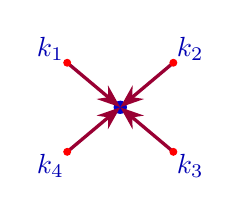
\begin{tikzpicture}[baseline=-0.6ex, scale=0.8, >=Stealth]
    \fill[blue!80!black] (0,0) circle (3pt);
    \foreach \ang/\lab in {140/k_1,40/k_2,-40/k_3,-140/k_4} {
      \draw[purple!80!black, very thick, ->]
        ({1.1*cos(\ang)},{1.1*sin(\ang)}) -- (0,0);
      \fill[red] ({1.1*cos(\ang)},{1.1*sin(\ang)}) circle (1.8pt);
      \node[blue!70!black] at ({1.45*cos(\ang)},{1.45*sin(\ang)}) {$\lab$};
    }
  \end{tikzpicture}
  +\cdots  \\
  &=
  (2\pi)^D
  \delta^D(k_1^E+k_2^E+k_3^E+k_4^E)
  \left[
    -g
    \prod_{j=1}^{4}
    \frac{1}{(k_j^E)^2+m^2}
    +O(g^2)
  \right].
\end{aligned}
\]
As above, one can write
\[
  m^2=m_R^2+\delta m^2
\]
and expand in \(\delta m^2\), regrouping the terms according to powers of
\(g\). A convenient choice is \(m_R=m_*\).

\subsection{Lorentzian Green Functions}

Everything said so far about the perturbative computation of
\[
  G_E(x_1^E,\ldots,x_n^E)
\]
can be equally applied to computing the time-ordered Green function
\[
  G(x_1,\ldots,x_n)
  =
  \langle\Omega|
  T\hat\phi(x_1)\cdots\hat\phi(x_n)
  |\Omega\rangle,
\]
with the modification of Feynman rules:
\[
\begin{array}{ccl}
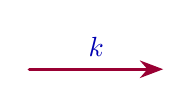
\begin{tikzpicture}[baseline=-0.5ex, scale=0.85, >=Stealth]
  \draw[purple!80!black, very thick, ->] (-1,0)--(1,0);
  \node[blue!70!black, above] at (0,0.05) {$k$};
\end{tikzpicture}
&=&
\displaystyle
\frac{-\ii}{k^2+m^2-\ii\epsilon},
\\[2.0em]
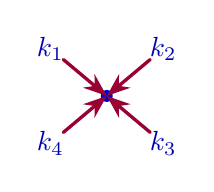
\begin{tikzpicture}[baseline=-0.6ex, scale=0.72, >=Stealth]
  \fill[blue!80!black] (0,0) circle (3pt);
  \foreach \ang/\lab in {140/k_1,40/k_2,-40/k_3,-140/k_4} {
    \draw[purple!80!black, very thick, ->]
      ({1.0*cos(\ang)},{1.0*sin(\ang)}) -- (0,0);
    \node[blue!70!black] at ({1.3*cos(\ang)},{1.3*sin(\ang)}) {$\lab$};
  }
\end{tikzpicture}
&=&
\displaystyle
-\frac{\ii g}{4!}\,
(2\pi)^D\delta^D(k_1+k_2+k_3+k_4).
\end{array}
\]
All momenta \(k^\mu\) are now Lorentzian, for example
\[
  k^2\equiv \eta_{\mu\nu}k^\mu k^\nu.
\]
For instance, the one-loop tadpole is
\[
\begin{tikzpicture}[baseline=-0.5ex, scale=0.75, >=Stealth]
  \draw[purple!80!black, very thick, ->] (-1.3,0)--(-0.05,0);
  \draw[purple!80!black, very thick, ->] (0.05,0)--(1.3,0);
  \draw[purple!80!black, very thick]
    (0,0) .. controls (-0.42,0.88) and (0.42,0.88) .. (0,0);
  \fill (0,0) circle (2.2pt);
  \node[blue!70!black] at (-1.0,-0.33) {$k$};
  \node[blue!70!black] at (1.0,-0.33) {$k$};
  \node[blue!70!black] at (0,0.92) {$k'$};
\end{tikzpicture}
=
-\frac{\ii g}{2}
\int\frac{\dd^Dk'}{(2\pi)^D}
\frac{-\ii}{k'^2+m^2-\ii\epsilon}.
\]
In the complex \((k')^0\)-plane this may be Wick rotated:
\begin{center}
\begin{tikzpicture}[baseline=-0.5ex, scale=0.95, >=Stealth]
  \draw[line width=0.55pt] (-2.65,-1.7) rectangle (2.65,1.7);
  \draw[->,green!50!black, thick] (-2.35,0)--(2.35,0) node[right] {$\mathbb R$};
  \draw[->,purple!80!black, thick] (0,-1.45)--(0,1.45);
  \node[purple!80!black, above] at (0,1.45) {cplx \((k')^0\)};
  \node[red] at (-1.35,0.32) {\(\times\)};
  \node[red] at (1.35,-0.32) {\(\times\)};
  \draw[->,orange!85!black, very thick]
    (1.05,1.08) .. controls (0.5,0.92) and (0.32,0.45) .. (-0.16,0.42);
  \draw[->,orange!85!black, very thick]
    (-1.05,-1.05) .. controls (-0.55,-0.9) and (-0.35,-0.45) .. (0.18,-0.42);
  \node[orange!85!black] at (1.25,1.05) {Wick rotation};
  \node[purple!80!black, right] at (2.55,1.15) {\((k')^0=\ii k^D\)};
\end{tikzpicture}
\end{center}
The rotation gives
\[
\begin{aligned}
-\frac{\ii g}{2}
\int\frac{\dd^Dk'}{(2\pi)^D}
\frac{-\ii}{k'^2+m^2-\ii\epsilon}
=
\ii\left[
-\frac{g}{2}
\int\frac{\dd^Dk_E'}{(2\pi)^D}
\frac{1}{(k_E')^2+m^2}
\right].
\end{aligned}
\]
Thus this contribution is to \(\ii\Sigma(k)\), consistently with the
Euclidean computation.

The full time-ordered two-point function takes the form
\[
  G(x,y)
  =
  \int\frac{\dd^Dk}{(2\pi)^D}
  \ee^{\ii k\cdot(x-y)}
  \widetilde G(k),
\]
where
\[
  \widetilde G(k)
  =
  \frac{-\ii}{k^2+m^2-\ii\epsilon-\Sigma(k)}.
\]
The function \(\Sigma(k)\) is expected to have a pair of branch cuts in
\(k^0\), starting at the multi-particle threshold
\[
  -k^2=M^2,
\]
where \(M\) is the invariant mass of the lightest multi-particle state.
These branch cuts may be chosen to extend along the real \(k^0\)-axis:
\[
  k^0>\sqrt{\vec k^2+M^2},
  \qquad
  k^0<-\sqrt{\vec k^2+M^2}.
\]

\begin{center}
\begin{tikzpicture}[scale=0.95, >=Stealth]
  \draw[line width=0.55pt] (-3.0,-2.0) rectangle (3.0,2.0);
  \draw[->,blue!70!black, thick] (-2.65,0)--(2.65,0)
    node[right] {$\operatorname{Re} k^0$};
  \draw[->,green!50!black, thick] (0,-1.75)--(0,1.75)
    node[above] {$\operatorname{Im} k^0$};
  \draw[red!80!black, very thick, decorate,
    decoration={zigzag,segment length=4pt,amplitude=1.2pt}]
    (-2.65,0)--(-1.0,0);
  \draw[red!80!black, very thick, decorate,
    decoration={zigzag,segment length=4pt,amplitude=1.2pt}]
    (1.0,0)--(2.65,0);
  \node[below] at (-1.0,-0.05)
    {$-\sqrt{\vec k^2+M^2}$};
  \node[below] at (1.0,-0.05)
    {$\sqrt{\vec k^2+M^2}$};
  \draw[->,orange!85!black, very thick]
    (1.55,1.0) .. controls (2.1,0.8) and (2.1,0.3) .. (1.55,0.12);
  \draw[->,orange!85!black, very thick]
    (-1.45,-1.0) .. controls (-2.05,-0.8) and (-2.05,-0.3) .. (-1.45,-0.12);
  \node[blue!70!black, anchor=west] at (-2.75,1.65) {cplx \(k^0\)};
\end{tikzpicture}
\end{center}

The actual value of \(\Sigma(k)\) at real \(k^0\) is determined by our Wick
rotation procedure relating \(G_E\) to \(G\). For example, for real
\[
  k^0>\sqrt{\vec k^2+M^2},
\]
\(\Sigma(k)\) is given by analytic continuation from \(k^0\in\ii\mathbb R\)
(or, more generally, complex \(k^0\) on the ``first sheet'') to the positive
real \(k^0\)-axis from above.

\section{Scattering Theory}

We now introduce in- and out-basis states.

\begin{center}
\begin{tikzpicture}[scale=0.95, >=Stealth]
  \draw[->, thick] (-3.3,-2.4)--(-3.3,2.5) node[above] {$t$};
  \draw[->, thick] (-3.3,-2.4)--(-1.1,-2.4) node[right] {$\vec x$};
  \fill[pattern=north east lines, pattern color=black!55, draw=black,
    line width=0.9pt] (0,0) ellipse (1.2 and 0.55);
  \draw[blue!75!black, dashed, thick] (-1.9,1.45)--(2.2,1.45);
  \draw[green!50!black, dashed, thick] (-1.9,-1.45)--(2.2,-1.45);
  \foreach \x in {-0.55,0.15,0.85} {
    \draw[->, blue!75!black, very thick]
      (\x,0.45)--({\x+0.55},1.55);
  }
  \foreach \x in {-0.55,0.55} {
    \draw[->, green!50!black, very thick]
      ({\x-0.55},-1.55)--(\x,-0.45);
  }
  \node[blue!75!black, align=left, anchor=west] at (2.45,1.45)
    {out-basis: states that look like far-separated\\
     (wave packets of) particles in the far future};
  \node[green!50!black, align=left, anchor=west] at (2.45,-1.45)
    {in-basis: states that look like far-separated\\
     particles in the far past};
\end{tikzpicture}
\end{center}

One can label out- or in-basis states as if they consist of free particles:
\[
  |\vec k_1,\vec k_2,\ldots,\vec k_n\rangle^{\mathrm{out}},
  \qquad
  |\vec k_1,\vec k_2,\ldots,\vec k_n\rangle^{\mathrm{in}}.
\]
For now we assume one particle species. Otherwise one also adds labels of
particle type and helicity, and so on.

Either the out-basis states \(|\alpha\rangle^{\mathrm{out}}\) or the in-basis
states \(|\alpha\rangle^{\mathrm{in}}\) span the entire Hilbert space
\(\mathcal H\). In an interacting QFT, the in- and out-bases are different,
and are related by a linear change of basis:
\[
  {}^{\mathrm{out}}\langle\beta|\alpha\rangle^{\mathrm{in}}
  \equiv S_{\beta\alpha},
\]
the \(S\)-matrix. Equivalently,
\[
  |\alpha\rangle^{\mathrm{in}}
  =
  \int\dd\beta\,
  S_{\beta\alpha}|\beta\rangle^{\mathrm{out}},
\]
with normalization
\[
  \int\dd\beta\,
  S_{\gamma\beta}^{\dagger}S_{\beta\alpha}
  =
  \delta_{\gamma\alpha}.
\]
Next we will give an explicit construction of in- or out-basis states using
the local field operator \(\hat\phi(x)\), thereby relating the \(S\)-matrix to
correlators of \(\hat\phi\). This is the Haag-Ruelle construction.

\subsection{Smeared Operators and One-Particle States}

Recall that
\[
\begin{aligned}
  \hat\phi(x)|\Omega\rangle
  &=
  \int\dd^{D-1}\vec k\,
  \ee^{-\ii\vec k\cdot\vec x+\ii\omega_{\vec k}x^0}
  \left[
    \frac{Z}{(2\pi)^{D-1}2\omega_{\vec k}}
  \right]^{1/2}
  |\vec k\rangle  \\
  &\quad
  +
  \int\dd\alpha\,
  \ee^{-\ii P_\alpha\cdot x}
  \langle\alpha|\hat\phi(0)|\Omega\rangle
  |\alpha\rangle .
\end{aligned}
\]
The second term is the multi-particle part. The multi-particle states are
separated from the one-particle states by a gap in their invariant masses.

Consider a smearing function \(f(x)\), \(x\in\mathbb R^{1,D-1}\), with
\[
  f(x)
  =
  \int\frac{\dd^Dk}{(2\pi)^D}\,\widetilde f(k)\,
  \ee^{\ii k\cdot x},
\]
such that \(\widetilde f(k)\) is supported near the mass shell
\[
  k^0>0,\qquad k^2+m^2=0,
\]
and at the same time \(f(x)\) is concentrated in a finite domain in spacetime.
For example, take the Gaussian profile
\[
\begin{aligned}
  f(x)
  &=
  \frac{1}{(2\pi)^{D/2}L^D}
  \exp\biggl[
    -\frac{1}{2L^2}(x^0-t_*)^2
    -\frac{1}{2L^2}(\vec x-\vec x_*)^2  \\
  &\hspace{3.7cm}
    +\ii\vec P_*\cdot(\vec x-\vec x_*)
    -\ii E_*(x^0-t_*)
  \biggr],
\end{aligned}
\]
for some large constant distance \(L>0\). Then
\[
  \widetilde f(k)
  =
  \exp\left[
    -\frac{L^2}{2}(k^0-E_*)^2
    -\frac{L^2}{2}(\vec k-\vec P_*)^2
    -\ii\vec k\cdot\vec x_*
    +\ii k^0t_*
  \right],
\]
peaked near
\[
  (k^0,\vec k)\simeq(E_*,\vec P_*),
\]
but still remembering \((t_*,\vec x_*)\).

A more convenient choice is to make \(\widetilde f(k)\) compactly supported
within a momentum domain of size \(\sim 1/L\), but still smooth. In that case
\(f(x)\) spreads to a blob of size \(\sim L\) and diminishes outside the blob
faster than \(|x|^{-N}\) for any \(N>0\) as \(|x|\to\infty\).

We further choose \((E_*,\vec P_*)\) such that
\[
  E_*^2-\vec P_*^{\,2}=m^2.
\]
Now consider the smeared operator
\[
  \hat\phi_f
  \equiv
  \int\dd^Dx\, f(x)\hat\phi(x).
\]
Then
\[
\begin{aligned}
  \hat\phi_f|\Omega\rangle
  &=
  \int\dd^{D-1}\vec k\,
  \widetilde f(\omega_{\vec k},\vec k)
  \left[
    \frac{Z}{(2\pi)^{D-1}2\omega_{\vec k}}
  \right]^{1/2}
  |\vec k\rangle \\
  &\quad
  +
  \int_{\mathrm{m.p.}}\dd\alpha\,
  \widetilde f(P_\alpha)
  \langle\alpha|\hat\phi(0)|\Omega\rangle
  |\alpha\rangle .
\end{aligned}
\]
The multi-particle contribution is suppressed by our choice of
\(\widetilde f(k)\), so only the one-particle state is retained.

Define the transformation \(f(x)\mapsto f^{(T)}(x)\) by setting
\[
  \widetilde f^{(T)}(k)
  :=
  \ee^{\ii(k^0-\omega_{\vec k})T}\widetilde f(k),
  \qquad
  \omega_{\vec k}=\sqrt{\vec k^2+m^2}.
\]
In particular,
\[
  \widetilde f^{(T)}(\omega_{\vec k},\vec k)
  =
  \widetilde f(\omega_{\vec k},\vec k),
\]
independent of \(T\). Therefore the one-particle part of
\(\hat\phi_{f^{(T)}}|\Omega\rangle\) is independent of \(T\). With the above
prescribed \(f(x)\), the multi-particle component of
\(\hat\phi_{f^{(T)}}|\Omega\rangle\) is negligible, and therefore
\[
  \hat\phi_{f^{(T)}}|\Omega\rangle
  \simeq
  \hat\phi_f|\Omega\rangle.
\]
The approximation is uniformly valid for all \(T\), including arbitrarily
large \(T\).

What does \(f^{(T)}(x)\) look like? By definition,
\[
  f^{(T)}(x)
  =
  \int\frac{\dd^Dk}{(2\pi)^D}\,
  \ee^{\ii k\cdot x+\ii(k^0-\omega_{\vec k})T}
  \widetilde f(k).
\]
Equivalently,
\[
\begin{aligned}
  f^{(T)}(x)
  &=
  \int\dd^Dy\,
  \int\frac{\dd^Dk}{(2\pi)^D}\,
  \ee^{\ii k\cdot(x-y)+\ii(k^0-\omega_{\vec k})T}
  f(y) \\
  &=
  \int\dd^Dy\,
  \delta(x^0-y^0-T)
  \int\frac{\dd^{D-1}\vec k}{(2\pi)^{D-1}}\,
  \ee^{\ii\vec k\cdot(\vec x-\vec y)-\ii\omega_{\vec k}T}
  f(y) \\
  &=
  \int\dd^{D-1}\vec y\,
  K(\vec x-\vec y;T)\,
  f(x^0-T,\vec y),
\end{aligned}
\]
where
\[
  K(\vec x;T)
  =
  \int\frac{\dd^{D-1}\vec k}{(2\pi)^{D-1}}\,
  \ee^{\ii\vec k\cdot\vec x-\ii\omega_{\vec k}T}.
\]
The kernel \(K(\vec x;T)\) obeys the Klein-Gordon equation
\[
  \left(
    \frac{\partial^2}{\partial\vec x^{\,2}}
    -
    \frac{\partial^2}{\partial T^2}
    -
    m^2
  \right)
  K(\vec x;T)=0,
\]
with initial condition
\[
  K(\vec x;0)=\delta^{D-1}(\vec x).
\]
If \(\widetilde f(k)\) is peaked at
\[
  k_*\simeq(E_*,\vec P_*),
\]
then \(f^{(T)}(x^0,\vec x)\) looks like the wave packet
\[
  f(x^0-T,\vec x)
\]
having moved with group velocity
\[
  \vec v
  =
  \frac{\partial\omega_{\vec P_*}}{\partial\vec P_*}
  =
  \frac{\vec P_*}{E_*}
\]
for time \(T\).

\begin{center}
\begin{tikzpicture}[scale=0.95, >=Stealth]
  \draw[->, thick] (-2.7,-1.65)--(-2.7,2.6) node[above] {$x^0$};
  \draw[->, thick] (-2.7,-1.65)--(3.2,-1.65) node[right] {$\vec x$};
  \fill[blue!8, draw=blue!80!black, very thick]
    (-0.7,-0.75) ellipse (0.95 and 0.55);
  \foreach \s in {-0.35,0,0.35} {
    \draw[blue!80!black, thick] (-1.2+\s,-1.0)--(-0.55+\s,-0.45);
  }
  \fill[purple!8, draw=purple!80!black, very thick]
    (1.45,1.35) ellipse (0.95 and 0.55);
  \foreach \s in {-0.35,0,0.35} {
    \draw[purple!80!black, thick] (0.95+\s,1.1)--(1.6+\s,1.65);
  }
  \draw[->, green!60!black, very thick] (-0.1,-0.25)--(1.15,0.95);
  \node[blue!80!black] at (0.35,-0.7) {$\operatorname{supp}(f)$};
  \node[purple!80!black] at (2.65,1.7)
    {$\operatorname{supp}(f^{(T)})$};
  \node[green!60!black] at (0.95,0.22) {$\Delta\vec x=\vec vT$};
  \draw[dashed, gray] (-1.75,-0.75)--(2.45,-0.75);
  \draw[dashed, gray] (0.1,1.35)--(2.45,1.35);
\end{tikzpicture}
\end{center}

Evolving \(f\mapsto f^{(T)}\), the support of \(f(x)\), say a region in
spacetime of large size \(\sim L\) centered around \((t_*,\vec x_*)\), moves
to a region centered around
\[
  (t_*+T,\vec x_*+\vec vT),
\]
and yet
\[
  \hat\phi_{f^{(T)}}|\Omega\rangle
  \simeq
  \hat\phi_f|\Omega\rangle.
\]
It is the same one-particle state. This may seem counterintuitive, but there
is no contradiction: there are a lot more operators than states.

Now consider a pair of functions \(f_1(x)\), \(f_2(x)\) of the above prescribed
form, whose Fourier transforms \(\widetilde f_1(k)\), \(\widetilde f_2(k)\)
are supported near \(k\simeq k_1,k_2\) respectively,
\[
  k_1^2=k_2^2=-m^2.
\]
Also assume
\[
  \vec k_1\neq \vec k_2 .
\]

\begin{center}
\begin{tikzpicture}[>=Stealth,scale=0.95]
  \begin{scope}[shift={(-3.7,0)}]
    \draw[->, thick] (0,-2.1)--(0,2.1) node[above] {$p^0$};
    \draw[->, thick] (0,-2.1)--(2.6,-3.0) node[below] {$p^1$};
    \draw[->, thick] (0,-2.1)--(3.0,-1.75) node[right] {$p^2$};
    \draw[blue!75!black, very thick]
      (-2.1,0.35) .. controls (-1.45,1.9) and (1.45,1.9) .. (2.1,0.35);
    \draw[blue!75!black, very thick]
      (-2.1,0.35) .. controls (-1.15,-0.15) and (1.15,-0.15) .. (2.1,0.35);
    \fill[purple!25,draw=purple!80!black,very thick]
      (-0.85,0.35) ellipse (0.32 and 0.22);
    \foreach \s in {-0.12,0.08}
      \draw[purple!80!black,thick] (-1.05+\s,0.23)--(-0.72+\s,0.48);
    \fill[green!25,draw=green!55!black,very thick]
      (1.05,0.55) ellipse (0.32 and 0.22);
    \foreach \s in {-0.12,0.08}
      \draw[green!55!black,thick] (0.85+\s,0.43)--(1.18+\s,0.68);
    \node[purple!80!black] at (-1.25,-0.2) {$k_1$};
    \node[green!55!black] at (1.75,0.57) {$\sim k_2$};
  \end{scope}

  \begin{scope}[shift={(3.4,-0.4)}]
    \draw[->, thick] (-2.2,-1.5)--(-2.2,2.1) node[above] {$x^0$};
    \draw[->, thick] (-2.2,-1.5)--(2.9,-1.5) node[right] {$\vec x$};
    \fill[blue!12,draw=blue!75!black,very thick]
      (-0.25,-1.3) ellipse (0.62 and 0.38);
    \fill[green!12,draw=green!55!black,very thick]
      (0.35,-1.3) ellipse (0.62 and 0.38);
    \fill[blue!12,draw=blue!75!black,very thick]
      (-0.75,0.75) ellipse (0.55 and 0.35);
    \fill[green!12,draw=green!55!black,very thick]
      (1.4,0.55) ellipse (0.55 and 0.35);
    \foreach \x/\c in {-0.25/blue!75!black,0.35/green!55!black,
                       -0.75/blue!75!black,1.4/green!55!black} {
      \draw[\c,thick] (\x-0.22,-1.42)--(\x+0.12,-1.18);
    }
    \draw[->,blue!75!black,thick] (-0.35,-0.95)--(-0.68,0.38);
    \draw[->,green!55!black,thick] (0.48,-0.95)--(1.18,0.25);
    \node[blue!75!black] at (-1.55,0.95) {$f_1^{(T)}$};
    \node[green!55!black] at (2.15,0.82) {$f_2^{(T)}$};
  \end{scope}
\end{tikzpicture}
\end{center}

The regions of concentration of \(f_1^{(T)}\) and \(f_2^{(T)}\) move apart as
\[
  T\to\pm\infty,
\]
and become far space-like separated.

\subsection{Multi-Particle In/Out States}

Consider the state
\[
  |\Psi^{(T)}\rangle
  \equiv
  \hat\phi_{f_1^{(T)}}\hat\phi_{f_2^{(T)}}|\Omega\rangle .
\]
The overlap between \(|\Psi^{(T)}\rangle\) and \(|\Psi^{(T')}\rangle\) is
\[
\begin{aligned}
  \langle\Psi^{(T)}|\Psi^{(T')}\rangle
  &=
  \langle\Omega|
  \hat\phi_{f_2^{(T)}*}
  \hat\phi_{f_1^{(T)}*}
  \hat\phi_{f_1^{(T')}}
  \hat\phi_{f_2^{(T')}}
  |\Omega\rangle .
\end{aligned}
\]
Fix
\[
  T'-T\equiv\Delta T,
  \qquad
  \text{send }T\to\pm\infty .
\]

\begin{center}
\begin{tikzpicture}[>=Stealth,scale=0.95]
  \draw[->,thick] (-3.3,-1.8)--(-3.3,2.0) node[above] {$x^0$};
  \draw[->,thick] (-3.3,-1.8)--(3.4,-1.8) node[right] {$\vec x$};
  \fill[purple!15,draw=purple!85!black,very thick] (-2.1,-1.1) ellipse (0.45 and 0.3);
  \fill[blue!12,draw=blue!75!black,very thick] (-1.45,0.65) ellipse (0.48 and 0.3);
  \fill[green!12,draw=green!55!black,very thick] (2.0,-1.0) ellipse (0.45 and 0.3);
  \fill[teal!12,draw=teal!70!black,very thick] (2.55,0.55) ellipse (0.48 and 0.3);
  \draw[<->,purple!80!black,very thick] (-0.8,0.15)--(1.2,0.0)
    node[midway,above,align=center] {large spacelike\\separation};
  \node[purple!85!black] at (-2.7,-0.72) {$f_1^{(T')}$};
  \node[blue!75!black] at (-2.0,1.08) {$f_1^{(T)}$};
  \node[green!55!black] at (2.6,-0.65) {$f_2^{(T')}$};
  \node[teal!70!black] at (3.1,0.95) {$f_2^{(T)}$};
\end{tikzpicture}
\end{center}

By the cluster property,
\[
\begin{aligned}
&\langle\Omega|
  \hat\phi_{f_2^{(T)}*}
  \hat\phi_{f_1^{(T)}*}
  \hat\phi_{f_1^{(T')}}
  \hat\phi_{f_2^{(T')}}
  |\Omega\rangle
\\
&\qquad\longrightarrow
  \langle\Omega|
  \hat\phi_{f_1^{(T)}*}
  \hat\phi_{f_1^{(T')}}
  |\Omega\rangle\,
  \langle\Omega|
  \hat\phi_{f_2^{(T)}*}
  \hat\phi_{f_2^{(T')}}
  |\Omega\rangle ,
\end{aligned}
\]
which is independent of \(\Delta T\). It follows that
\[
  \bigl\|\,|\Psi^{(T')}\rangle-|\Psi^{(T)}\rangle\,\bigr\|
  \longrightarrow 0
  \qquad
  \text{as }T\to\pm\infty .
\]
In fact, with non-overlapping and smooth \(\widetilde f_i(k)\), this norm
vanishes faster than \(|T|^{-N}\) for any \(N>0\) as \(T\to\pm\infty\)
\((\text{Hepp }1965)\).

Thus
\[
  \lim_{T\to\pm\infty}
  \hat\phi_{f_1^{(T)}}\hat\phi_{f_2^{(T)}}|\Omega\rangle
  :=
  |\phi_{f_1},\phi_{f_2}\rangle^{\mathrm{out/in}}
\]
is a well-defined state in \(\mathcal H\). Compare this with
\[
  \hat\phi_f|\Omega\rangle
  =
  \int\dd^{D-1}\vec k\,
  \widetilde f(\omega_{\vec k},\vec k)
  \left[
    \frac{Z}{(2\pi)^{D-1}2\omega_{\vec k}}
  \right]^{1/2}
  |\vec k\rangle ,
\]
assuming \(\operatorname{supp}\widetilde f\) is concentrated near the
one-particle mass shell, with no overlap with the multi-particle momentum
region. We can write
\[
\begin{aligned}
  |\phi_{f_1},\phi_{f_2}\rangle^{\mathrm{out/in}}
  &=
  \int\prod_{j=1}^2 \dd^{D-1}\vec k_j\,
  \widetilde f_j(\omega_{\vec k_j},\vec k_j)
  \left[
    \frac{Z}{(2\pi)^{D-1}2\omega_{\vec k_j}}
  \right]^{1/2}
  |\vec k_1,\vec k_2\rangle^{\mathrm{out/in}} .
\end{aligned}
\]

Using the cluster property, one can verify that
\(|\vec k_1,\vec k_2\rangle^{\mathrm{out/in}}\) obey the orthogonality
\[
\begin{aligned}
  {}^{\mathrm{out}}\langle
  \vec k_1,\vec k_2|\vec k_1',\vec k_2'
  \rangle^{\mathrm{out}}
  &=
  \delta^{D-1}(\vec k_1-\vec k_1')\,
  \delta^{D-1}(\vec k_2-\vec k_2')
  +(\vec k_1'\leftrightarrow\vec k_2'),
\end{aligned}
\]
and the same with
\[
  {}^{\mathrm{in}}\langle
  \vec k_1,\vec k_2|\vec k_1',\vec k_2'
  \rangle^{\mathrm{in}} .
\]

The generalization to \(n\)-particle in/out-states
\[
  |\vec k_1,\ldots,\vec k_n\rangle^{\mathrm{in/out}}
\]
is obvious. Given \(f_1(x),\ldots,f_n(x)\) whose Fourier transforms
\(\widetilde f_1(k),\ldots,\widetilde f_n(k)\) are supported near the mass
shell
\[
  k^2+m^2=0,
  \qquad
  k^0>0,
\]
and do not overlap,
\[
\begin{aligned}
  \lim_{T\to\pm\infty}
  \hat\phi_{f_1^{(T)}}\cdots\hat\phi_{f_n^{(T)}}|\Omega\rangle
  &:=
  |\phi_{f_1},\ldots,\phi_{f_n}\rangle^{\mathrm{out/in}} \\
  &=
  \int\prod_{j=1}^n \dd^{D-1}\vec k_j\,
  \widetilde f_j(\omega_{\vec k_j},\vec k_j)
  \left[
    \frac{Z}{(2\pi)^{D-1}2\omega_{\vec k_j}}
  \right]^{1/2}
  |\vec k_1,\ldots,\vec k_n\rangle^{\mathrm{out/in}} .
\end{aligned}
\]
The normalization is such that
\[
\begin{aligned}
  {}^{\mathrm{out}}\langle
  \vec k_1,\ldots,\vec k_n
  |\vec k_1',\ldots,\vec k_m'
  \rangle^{\mathrm{out}}
  &=
  \delta_{nm}
  \sum_{\sigma\in S_n}
  \prod_{j=1}^n
  \delta^{D-1}(\vec k_j-\vec k_{\sigma(j)}'),
\end{aligned}
\]
and the same for
\[
  {}^{\mathrm{in}}\langle\cdots|\cdots\rangle^{\mathrm{in}} .
\]

\subsection{LSZ Reduction}

The \(S\)-matrix elements are defined as
\[
  S(\vec k_1,\ldots,\vec k_n|\vec k_1',\ldots,\vec k_m')
  =
  {}^{\mathrm{out}}\langle
  \vec k_1,\ldots,\vec k_n
  |\vec k_1',\ldots,\vec k_m'
  \rangle^{\mathrm{in}} .
\]
The generalization to more than one species of particles is obvious. By
construction, the \(S\)-matrix elements are determined by a suitable limit of
integrated Wightman functions. Let us inspect this relation in more detail:
\[
\begin{aligned}
&{}^{\mathrm{out}}\langle
  \phi_{f_1},\ldots,\phi_{f_n}
  |\phi_{g_1},\ldots,\phi_{g_m}
  \rangle^{\mathrm{in}}
\\
&=
  \int
  \prod_{i=1}^n \dd^{D-1}\vec k_i\,
  \widetilde f_i^*(\omega_{\vec k_i},\vec k_i)
  \left[
    \frac{Z}{(2\pi)^{D-1}2\omega_{\vec k_i}}
  \right]^{1/2}
\\
&\quad\times
  \prod_{j=1}^m \dd^{D-1}\vec k_j'\,
  \widetilde g_j(\omega_{\vec k_j'},\vec k_j')
  \left[
    \frac{Z}{(2\pi)^{D-1}2\omega_{\vec k_j'}}
  \right]^{1/2}
  S(\vec k_1,\ldots,\vec k_n|\vec k_1',\ldots,\vec k_m') .
\end{aligned}
\]
The left hand side, by definition, is
\[
\begin{aligned}
&\lim_{T\to\infty}
  \langle\Omega|
  \hat\phi_{f_n^{(T)}*}\cdots\hat\phi_{f_1^{(T)}*}
  \hat\phi_{g_1^{(-T)}}\cdots\hat\phi_{g_m^{(-T)}}|\Omega\rangle
\\
&=
  \lim_{T\to\infty}
  \langle\Omega|
  T\!\left[
  \hat\phi_{f_1^{(T)}*}\cdots
  \hat\phi_{f_n^{(T)}*}
  \hat\phi_{g_1^{(-T)}}\cdots
  \hat\phi_{g_m^{(-T)}}\right]
  |\Omega\rangle ,
\end{aligned}
\]
where the two groups of wave packets are asymptotically spacelike separated.

\begin{center}
\begin{tikzpicture}[>=Stealth,scale=0.92]
  \draw[->,thick] (-2.5,-2.0)--(-2.5,2.0) node[above] {$x^0$};
  \draw[->,thick] (-2.5,-2.0)--(3.0,-2.0) node[right] {$\vec x$};
  \foreach \x/\lab in {-1.2/f_1,-0.35/f_2,0.5/f_n} {
    \fill[blue!12,draw=blue!75!black,thick] (\x,0.95) ellipse (0.22 and 0.16);
    \node[blue!75!black] at (\x,1.35) {$\lab$};
  }
  \foreach \x/\lab in {-1.2/g_1,-0.35/g_2,0.5/g_m} {
    \fill[green!12,draw=green!55!black,thick] (\x,-0.85) ellipse (0.22 and 0.16);
    \node[green!55!black] at (\x,-1.2) {$\lab$};
  }
  \draw[<->,purple,very thick] (1.45,-0.75)--(1.45,0.92)
    node[midway,right] {$2T$};
  \node[blue!75!black,align=center] at (-0.35,1.8)
    {asymp. spacelike\\separated};
  \node[green!55!black,align=center] at (2.55,0.05)
    {asymp. spacelike\\separated};
\end{tikzpicture}
\end{center}

Equivalently,
\[
\begin{aligned}
&\lim_{T\to\infty}
  \int \dd^Dx_1\,f_1^{(T)*}(x_1)\cdots
  \dd^Dy_1\,g_1^{(-T)}(y_1)\cdots
\\
&\qquad\qquad\times
  \langle\Omega|T\hat\phi(x_1)\cdots\hat\phi(y_1)\cdots|\Omega\rangle
\\
&=
  \lim_{T\to\infty}
  \int
  \frac{\dd^Dk_1}{(2\pi)^D}\,
  \widetilde f_1^*(k_1)\,
  \ee^{-\ii(k_1^0-\omega_{\vec k_1})T}\cdots
\\
&\quad\times
  \frac{\dd^Dk_1'}{(2\pi)^D}\,
  \widetilde g_1(-k_1')\,
  \ee^{\ii(-k_1'{}^0-\omega_{\vec k_1'})(-T)}\cdots
  \widetilde G(k_1,\ldots,k_n,k_1',\ldots,k_m') .
\end{aligned}
\]
The \(T\to\infty\) limit of the \(k_i^0,k_j'{}^0\)-integral vanishes unless
\(\widetilde G\) is singular at
\[
  k_i^0=\omega_{\vec k_i},
  \qquad
  k_j'{}^0=-\omega_{\vec k_j'} .
\]
Compare the perturbative computation of \(\widetilde G\):
\[
  \widetilde G(k)
  =
  \frac{-\ii}{k^2+m_0^2-\ii\epsilon-\Sigma(k)} ,
\]
with bare mass \(m_0\), and pole at
\[
  k^2=-m_*^2
\]
for the physical mass \(m_*\).

For example,
\[
\begin{aligned}
&\lim_{T\to\infty}
  \int\frac{\dd^Dk}{(2\pi)^D}\,
  \frac{\widetilde g(-k)\,
  \ee^{\ii(-k^0-\omega_{\vec k})(-T)}}{k^2+m^2-\ii\epsilon}
\\
&\quad =
  \int\frac{\dd^{D-1}\vec k}{(2\pi)^{D-1}}\,
  \widetilde g(\omega_{\vec k},-\vec k)
  \lim_{T\to\infty}
  \int\frac{\dd k^0}{2\pi}\,
  \frac{\ee^{\ii(-k^0-\omega_{\vec k})(-T)}}{k^2+m^2-\ii\epsilon}
\\
&\quad =
  \int\frac{\dd^{D-1}\vec k}{(2\pi)^{D-1}}\,
  \widetilde g(\omega_{\vec k},-\vec k)\,
  \frac{\ii}{2\omega_{\vec k}},
\end{aligned}
\]
where the contour integral is dominated by the residue at
\[
  k^0=-\omega_{\vec k}+\ii\epsilon .
\]
Similarly,
\[
\begin{aligned}
&\lim_{T\to\infty}
  \int\frac{\dd^Dk}{(2\pi)^D}\,
  \frac{\widetilde f^*(k)\,
  \ee^{-\ii(k^0-\omega_{\vec k})T}}{k^2+m^2-\ii\epsilon}
\\
&\quad =
  \int\frac{\dd^{D-1}\vec k}{(2\pi)^{D-1}}\,
  \widetilde f^*(\omega_{\vec k},\vec k)\,
  \frac{\ii}{2\omega_{\vec k}} .
\end{aligned}
\]

The time-ordered Green function \(G(x_1,\ldots,x_n)\) takes the form
\[
  \sum \prod G_{\mathrm{conn}},
\]
where \(G_{\mathrm{conn}}(x_i,\ldots,x_j)\) decays at large spacelike
separation (cluster property). After Fourier transform, each
\(\widetilde G_{\mathrm{conn}}(\{\text{subset of }k_i\})\) contains a
momentum-\(\delta\)-function.

In taking the \(T\to\infty\) limit above, the momentum \(\delta\)-functions in
\(\widetilde G\) come along with the ride, with one exceptional case:

\begin{center}
\begin{tikzpicture}[>=Stealth,scale=0.95]
  \begin{scope}
    \draw[thick] (-2.1,0.65)--(-0.7,0.65);
    \draw[thick,->] (-2.0,0.65)--(-1.45,0.65) node[above] {$k_1$};
    \draw[thick] (0.7,0.65)--(2.1,0.65);
    \draw[thick,->] (1.9,0.65)--(1.35,0.65) node[above] {$k_1'$};
    \fill[blue!25,draw=blue!80!black,thick] (0,0.65) circle (0.28);
    \draw[thick] (-2.0,-0.85)--(-0.85,-0.45)--(0,-0.45);
    \draw[thick] (-2.0,-1.25)--(-0.85,-0.85)--(0,-0.85);
    \draw[thick] (0,-0.65)--(1.25,-0.95)--(2.1,-0.95);
    \draw[dashed,thick] (0.35,-0.45)--(1.1,-0.15);
    \draw[decorate,decoration={brace,amplitude=4pt,mirror}]
      (-2.2,-1.45)--(2.25,-1.45);
    \node at (0,-1.82) {$\dfrac{-\ii Z}{k_1^2+m^2-\ii\epsilon}$};
  \end{scope}
  \node[anchor=west] at (3.0,0.35)
    {$+\;(\text{non-singular at }k_1^2=-m^2)$};
\end{tikzpicture}
\end{center}

This gives
\[
\begin{aligned}
&\lim_{T\to\infty}
  \int\frac{\dd^Dk}{(2\pi)^D}\,
  \widetilde f^*(k)\,
  \ee^{-\ii(k^0-\omega_{\vec k})T}
  \frac{\dd^Dk'}{(2\pi)^D}\,
  \widetilde g(-k')\,
  \ee^{\ii(-k'{}^0-\omega_{\vec k'})(-T)}
\\
&\qquad\qquad\times
  (2\pi)^D\delta^D(k+k')\,
  \frac{-\ii Z}{k^2+m^2-\ii\epsilon}
\\
&=
  \lim_{T\to\infty}
  \int\frac{\dd^Dk}{(2\pi)^D}\,
  \widetilde f^*(k)\widetilde g(k)\,
  \ee^{-2\ii(k^0-\omega_{\vec k})T}
  \frac{-\ii Z}{k^2+m^2-\ii\epsilon}
\\
&=
  \int\frac{\dd^{D-1}\vec k}{(2\pi)^{D-1}}\,
  \widetilde f^*(\omega_{\vec k},\vec k)\,
  \widetilde g(\omega_{\vec k},\vec k)\,
  \frac{Z}{2\omega_{\vec k}}
  =
  \langle\phi_f|\phi_g\rangle ,
\end{aligned}
\]
as expected.

Lehmann--Symanzik--Zimmermann (LSZ) reduction formula: compare with the
definition of the \(S\)-matrix elements. We conclude that
\[
\begin{aligned}
&S(\vec k_1,\ldots,\vec k_n|-\vec k_1',\ldots,-\vec k_m')
\\
&=
  \prod_{i=1}^n
  \left[Z(2\pi)^{D-1}2\omega_{\vec k_i}\right]^{-1/2}
  \prod_{j=1}^m
  \left[Z(2\pi)^{D-1}2\omega_{\vec k_j'}\right]^{-1/2}
\\
&\quad\times
  \lim_{\substack{
    k_i^0\to\omega_{\vec k_i}\\
    k_j'{}^0\to-\omega_{\vec k_j'}
  }}
  \prod_{i=1}^n \ii(k_i^2+m^2)
  \prod_{j=1}^m \ii(k_j'{}^2+m^2)\,
  \widetilde G(k_1,\ldots,k_n,k_1',\ldots,k_m') .
\end{aligned}
\]
With the exception of disconnected terms in \(\widetilde G\) that contain
\(\delta^D(k_i+k_j')\), which gives rise to disconnected factors
\(\delta^{D-1}(\vec k_i-\vec k_j')\) in \(S\), as discussed above.

It follows from the cluster property of Green functions and LSZ that the
\(S\)-matrix elements also obey a cluster property:
\[
  S(\beta|\alpha)
  \equiv
  {}^{\mathrm{out}}\langle\beta|\alpha\rangle^{\mathrm{in}}
  =
  \sum_{\substack{\alpha=\bigsqcup_I\alpha_I\\
                  \beta=\bigsqcup_I\beta_I}}
  \prod_I S^{\mathrm{conn}}(\beta_I|\alpha_I).
\]

\begin{center}
\begin{tikzpicture}[>=Stealth,scale=0.92]
  \node at (-4.3,0.2) {$\beta$};
  \node at (-4.3,-0.95) {$\alpha$};
  \draw[thick] (-3.7,0.55)--(-2.6,0.25);
  \draw[thick] (-3.7,0.15)--(-2.6,0.12);
  \draw[thick] (-3.7,-0.25)--(-2.6,-0.02);
  \draw[thick] (-3.7,-0.8)--(-2.6,-0.35);
  \draw[thick] (-3.7,-1.2)--(-2.6,-0.55);
  \node[circle,draw,thick,minimum size=1.3cm] at (-2.1,-0.2) {$S$};
  \draw[thick] (-1.45,0.22)--(-0.55,0.52);
  \draw[thick] (-1.45,0.02)--(-0.55,0.06);
  \draw[thick] (-1.45,-0.25)--(-0.55,-0.25);
  \node at (-0.1,-0.2) {$=$};

  \node[circle,draw,thick,minimum size=0.85cm] at (1.0,0.3) {$S^c$};
  \draw[thick] (0.0,0.6)--(0.58,0.48);
  \draw[thick] (0.0,0.25)--(0.58,0.32);
  \draw[thick] (1.42,0.38)--(2.0,0.55);
  \draw[thick] (1.42,0.2)--(2.0,0.15);
  \node at (2.35,0.25) {$+$};
  \node[circle,draw,thick,minimum size=0.85cm] at (3.25,0.35) {$S^c$};
  \draw[thick] (2.55,0.55)--(2.9,0.45);
  \draw[thick] (3.6,0.45)--(4.15,0.55);
  \node at (4.55,0.25) {$+\cdots$};
  \node[circle,draw,thick,minimum size=0.85cm] at (1.0,-1.0) {$S^c$};
  \draw[thick] (0.0,-1.25)--(0.58,-1.1);
  \draw[thick] (0.0,-0.88)--(0.58,-0.95);
  \draw[thick] (1.42,-1.0)--(2.0,-1.0);
\end{tikzpicture}
\end{center}

Each connected \(S\)-matrix element comes with a momentum \(\delta\)-function:
\[
\begin{aligned}
&S^{\mathrm{conn}}
  (\vec k_1,\ldots,\vec k_n|\vec k_1',\ldots,\vec k_m')
\\
&\quad =
  \ii(2\pi)^D
  \delta^D(k_1+\cdots+k_n-k_1'-\cdots-k_m')\,
  \mathcal M(\vec k_1,\ldots,\vec k_n|\vec k_1',\ldots,\vec k_m') ,
\end{aligned}
\]
where this is a convention, subject to
\[
  k_i^2=k_j'{}^2=-m^2,
  \qquad
  k_1+\cdots+k_n=k_1'+\cdots+k_m' .
\]

A more precise connected version of the LSZ formula is
\[
\begin{aligned}
&S^{\mathrm{conn}}
  (\vec k_1,\ldots,\vec k_n|-\vec k_1',\ldots,-\vec k_m')
\\
&\quad =
  \prod_{i=1}^n
  \left[Z(2\pi)^{D-1}2\omega_{\vec k_i}\right]^{-1/2}
  \prod_{j=1}^m
  \left[Z(2\pi)^{D-1}2\omega_{\vec k_j'}\right]^{-1/2}
\\
&\qquad\times
  \lim_{\substack{k_i^0\to \omega_{\vec k_i}\\
                  k_j'{}^0\to-\omega_{\vec k_j'}}}
  \prod_{i=1}^n \ii(k_i^2+m^2)
  \prod_{j=1}^m \ii(k_j'{}^2+m^2)\,
  \widetilde G^{\mathrm{conn}}
  (k_1,\ldots,k_n,k_1',\ldots,k_m')
\end{aligned}
\]
for \(n,m\ge 2\).

Due to our normalization convention for one-particle states, it is
convenient to further define
\[
\begin{aligned}
&M(\vec k_1,\ldots,\vec k_n|\vec k_1',\ldots,\vec k_m')
\\
&\quad \equiv
  \prod_{i=1}^n
  \frac{1}{(2\pi)^{(D-1)/2}\sqrt{2\omega_{\vec k_i}}}
  \prod_{j=1}^m
  \frac{1}{(2\pi)^{(D-1)/2}\sqrt{2\omega_{\vec k_j'}}}
  \mathcal A(k_1,\ldots,k_n|k_1',\ldots,k_m') .
\end{aligned}
\]
The amplitude \(\mathcal A\) is invariant under Lorentz transformations
\(k\mapsto \Lambda k\).

For example, in \(2\to2\) scattering, let
\[
  \alpha=\{\vec k_1',\vec k_2'\},
  \qquad
  \beta=\{\vec k_1,\vec k_2\}.
\]
Then
\[
\begin{aligned}
&S(\vec k_1,\vec k_2|\vec k_1',\vec k_2')
  \equiv
  {}^{\mathrm{out}}\langle \vec k_1,\vec k_2
  |\vec k_1',\vec k_2'\rangle^{\mathrm{in}}
\\
&\quad =
  \delta^{D-1}(\vec k_1-\vec k_1')
  \delta^{D-1}(\vec k_2-\vec k_2')
  +
  \delta^{D-1}(\vec k_1-\vec k_2')
  \delta^{D-1}(\vec k_2-\vec k_1')
\\
&\qquad
  +\ii(2\pi)^D
  \delta^D(k_1+k_2-k_1'-k_2')\,
  M(\vec k_1,\vec k_2|\vec k_1',\vec k_2') .
\end{aligned}
\]
Diagrammatically, the last term is the connected scattering process:
\[
\begin{tikzpicture}[baseline=-0.3ex,>=Stealth,scale=0.85]
  \draw[thick,->] (-1.7,0.75)--(-0.55,0.25);
  \draw[thick,->] (-1.7,-0.75)--(-0.55,-0.25);
  \draw[thick,->] (0.55,0.25)--(1.7,0.75);
  \draw[thick,->] (0.55,-0.25)--(1.7,-0.75);
  \node[circle,draw,thick,minimum size=0.95cm,pattern=north east lines] at (0,0) {};
  \node[left] at (-1.7,0.75) {$k_1'$};
  \node[left] at (-1.7,-0.75) {$k_2'$};
  \node[right] at (1.7,0.75) {$k_1$};
  \node[right] at (1.7,-0.75) {$k_2$};
\end{tikzpicture}
\]

\subsection*{\(\phi^4\) Theory}

In perturbative \(\phi^4\) theory, the connected four-point Green function is
represented at leading order by the contact vertex
\[
\begin{tikzpicture}[baseline=-0.4ex,>=Stealth,scale=0.72]
  \node[circle,draw,thick,minimum size=0.9cm,pattern=north east lines] at (0,0) {};
  \foreach \a in {45,135,225,315}
    \draw[thick] (0,0)--({1.0*cos(\a)},{1.0*sin(\a)});
  \foreach \a in {45,135,225,315}
    \fill ({1.0*cos(\a)},{1.0*sin(\a)}) circle (1.7pt);
\end{tikzpicture}
\quad = \quad
\begin{tikzpicture}[baseline=-0.4ex,>=Stealth,scale=0.72]
  \draw[thick] (-0.8,-0.8)--(0.8,0.8);
  \draw[thick] (-0.8,0.8)--(0.8,-0.8);
  \fill (0,0) circle (2pt);
  \node[above] at (0,0.12) {$g$};
\end{tikzpicture}
\quad +\quad O(g^2).
\]
More explicitly,
\[
\begin{aligned}
\widetilde G^{\mathrm{conn}}(k_1,k_2,k_3,k_4)
  &=
  (2\pi)^D\delta^D(k_1+\cdots+k_4)
  \left[
    (-\ii g)
    \prod_{j=1}^4
    \frac{-\ii}{k_j^2+m^2-\ii\epsilon}
    +O(g^2)
  \right],
\\
  Z&=1+O(g^2).
\end{aligned}
\]
The LSZ formula therefore gives
\[
\begin{aligned}
S^{\mathrm{conn}}(\vec k_1,\vec k_2|-\vec k_1',-\vec k_2')
&=
\ii(2\pi)^D
\delta^{D-1}(\vec k_1+\vec k_2-\vec k_1'-\vec k_2')
\\
&\quad\times
\delta(\omega_{\vec k_1}+\omega_{\vec k_2}
       -\omega_{\vec k_1'}-\omega_{\vec k_2'})
       \bigl[-\ii g+O(g^2)\bigr],
\end{aligned}
\]
and hence
\[
  \ii\,\mathcal A(k_1,k_2|k_1',k_2')=-\ii g+O(g^2).
\]
The higher-order terms include the \(s\), \(t\), and \(u\) channel
diagrams, as well as the correction to the factor \(Z^{-2}\).

\subsection*{\(S\)-Matrix as a Unitary Operator}

Recall that
\[
  S_{\beta\alpha}\equiv{}^{\mathrm{out}}\langle\beta|\alpha\rangle^{\mathrm{in}}.
\]
Define the operator \(\widehat S\) by
\[
  \widehat S|\alpha\rangle^{\mathrm{out}}
  =
  |\alpha\rangle^{\mathrm{in}}.
\]
Then
\[
  {}^{\mathrm{out}}\langle\beta|\widehat S|\alpha\rangle^{\mathrm{out}}
  =
  S_{\beta\alpha}.
\]
The operator \(\widehat S\) preserves the inner product:
\[
\begin{aligned}
{}^{\mathrm{in}}\langle\alpha|\alpha'\rangle^{\mathrm{in}}
&=
{}^{\mathrm{out}}\langle\alpha|\alpha'\rangle^{\mathrm{out}}
\\
&=
{}^{\mathrm{out}}\langle\alpha|\widehat S^\dagger\widehat S
|\alpha'\rangle^{\mathrm{out}},
\end{aligned}
\]
so
\[
  \widehat S^\dagger\widehat S=1
  \qquad
  (=\widehat S\widehat S^\dagger),
\]
i.e. \(\widehat S\) is a unitary operator on \(\mathcal H\).

Pick an orthonormal out-basis \(|\alpha\rangle^{\mathrm{out}}\) such that
\[
  {}^{\mathrm{out}}\langle\beta|\alpha\rangle^{\mathrm{out}}
  =
  \delta_{\beta\alpha},
  \qquad
  \int d\alpha\,
  |\alpha\rangle^{\mathrm{out}}{}^{\mathrm{out}}\langle\alpha|
  =
  1 .
\]
Unitarity is equivalently
\[
  \int d\gamma\, (S_{\gamma\beta})^*S_{\gamma\alpha}
  =
  \delta_{\beta\alpha}.
\]

\subsection*{Transition Probabilities and Cross Sections}

The state \(|\alpha\rangle^{\mathrm{in}}\) is the state that ``looks like''
far-separated incoming particles with momenta
\(\alpha=\{\vec k_1,\ldots,\vec k_n\}\) in the far past. The probability of
finding the state consisting of outgoing particles with momenta distributed in
the range \(\beta=\{\vec k_1',\ldots,\vec k_m'\}\in\mathcal D\) is
\[
  P_{\alpha\to\mathcal D}
  =
  \int_{\mathcal D}d\beta\, |S_{\beta\alpha}|^2.
\]
We have defined the scattering amplitude \(M\) by
\[
  S_{\beta\alpha}
  \equiv
  S^{\mathrm{free}}_{\beta\alpha}
  +\ii(2\pi)^D\delta^D(P_\beta-P_\alpha)M_{\beta\alpha}.
\]
Assuming \(\alpha\notin\mathcal D\),
\[
\begin{aligned}
P_{\alpha\to\mathcal D}
&=
\int_{\mathcal D}d\beta\,
\left|(2\pi)^D\delta^D(P_\beta-P_\alpha)M_{\beta\alpha}\right|^2
\\
&=
(2\pi)^D\delta^D(0)
\int_{\mathcal D}d\beta\,
(2\pi)^D\delta^D(P_\beta-P_\alpha)|M_{\beta\alpha}|^2 .
\end{aligned}
\]
Here
\[
  (2\pi)^D\delta^D(0)=V\,T
\]
is the volume of spacetime. This spacetime-volume divergence is no
contradiction, since we assumed that \(|\alpha\rangle^{\mathrm{in}}\) has
definite energy-momentum \(P_\alpha\), and hence is not a normalizable state.
For example, for a two-particle in-state
\[
  |\alpha\rangle^{\mathrm{in}}
  =
  |\vec k_1,\vec k_2\rangle^{\mathrm{in}},
  \qquad
  \vec k_1\ne \vec k_2,
\]
we have
\[
  {}^{\mathrm{in}}\langle \vec k_1,\vec k_2
  |\vec k_1,\vec k_2\rangle^{\mathrm{in}}
  =
  \delta^{D-1}(0)\,\delta^{D-1}(0)
  =
  \left(\frac{V}{(2\pi)^{D-1}}\right)^2.
\]

The transition rate per unit volume is
\[
  \Gamma_{\alpha\to\mathcal D}
  \equiv
  \frac{P_{\alpha\to\mathcal D}}{VT}
  =
  \int_{\mathcal D}d\beta\,
  (2\pi)^D\delta^D(P_\beta-P_\alpha)|M_{\beta\alpha}|^2 .
\]

\begin{center}
\begin{tikzpicture}[>=Stealth,scale=0.9]
  \draw[very thick,blue,->] (-4.0,-1.15)--(-2.1,-1.15);
  \node[blue,below] at (-3.1,-1.15) {particle \(1\)};
  \node[blue,above] at (-3.25,-1.05) {$\vec v_1$};
  \draw[very thick,green!50!black,->] (-1.0,0.55)--(-2.05,0.55);
  \node[green!50!black,above] at (-1.55,0.62) {particle \(2\)};
  \node[green!50!black,below] at (-1.45,0.45) {$\vec v_2$};
  \draw[purple,thick,fill=purple!9] (-1.9,-0.85)
    ellipse [x radius=0.34,y radius=1.0];
  \draw[purple,thick] (-2.08,-1.55)--(-1.75,0.05);
  \draw[purple,thick] (-2.0,-1.35)--(-1.66,0.25);
  \draw[purple,thick] (-1.93,-1.1)--(-1.61,0.45);
  \node[purple,below] at (-1.9,-1.9) {cross section};
  \node[purple,below] at (-1.9,-2.35) {area \(=\sigma\)};
  \node[purple] at (1.8,0.65) {relative velocity};
  \node[purple] at (1.8,0.15) {(in lab frame)};
  \node[purple] at (1.8,-0.55) {$v\equiv |\vec v_1-\vec v_2|$};
\end{tikzpicture}
\end{center}

The scattering cross section \(\sigma_{\mathcal D}\) is defined such that the
probability ratio of scattering into \(\beta\in\mathcal D\) is
\[
  \frac{\sigma_{\mathcal D}vT}{V},
\]
where \(\sigma_{\mathcal D}vT\) is the effective volume passing through
\(\sigma_{\mathcal D}\), while \(V\) is the total volume of space. Hence
\[
  \Gamma_{\alpha\to\mathcal D}
  =
  \frac{P_{\alpha\to\mathcal D}}{VT}
  =
  \frac{\sigma_{\mathcal D}v}{(2\pi)^{2D-2}},
\]
and therefore
\[
  \sigma_{\mathcal D}
  =
  \frac{(2\pi)^{2D-2}}{v}
  \int_{\mathcal D}d\beta\,
  (2\pi)^D\delta^D(P_\beta-P_\alpha)|M_{\beta\alpha}|^2 .
\]

For instance, consider \(2\to2\) scattering in \(D=4\), and take the total
cross section into a two-particle final state of identical particles. Then
\[
\begin{aligned}
\sigma_{2\to2}
&=
\frac{(2\pi)^6}{v}\,
\frac12
\int d^3\vec k_1'\,d^3\vec k_2'\,
(2\pi)^4\delta^4(k_1'+k_2'-k_1-k_2)
\\
&\qquad\qquad\qquad\qquad\times
\left|M(\vec k_1',\vec k_2'|\vec k_1,\vec k_2)\right|^2
\\
&=
\frac{(2\pi)^6}{
  \frac{|\vec k_1|}{\omega_{\vec k_1}}
  +
  \frac{|\vec k_2|}{\omega_{\vec k_2}}
}
\frac12
\int d^3\vec k_1'\,
(2\pi)^4
\delta(\omega_{\vec k_1'}+\omega_{\vec k_2'}-E)
\\
&\qquad\times
\frac{
  \left|\mathcal A(k_1',k_2'|k_1,k_2)\right|^2
}{
  (2\pi)^{12}\,2^4\,
  \omega_{\vec k_1'}\omega_{\vec k_2'}
  \omega_{\vec k_1}\omega_{\vec k_2}
},
\end{aligned}
\]
where
\[
  \vec k_2'=\vec k_1+\vec k_2-\vec k_1',
  \qquad
  E=\omega_{\vec k_1}+\omega_{\vec k_2}.
\]
In the center-of-mass frame,
\[
  \vec k_1+\vec k_2=0=\vec k_1'+\vec k_2',
\]
and
\[
  v=
  \frac{|\vec k_1|}{\omega_{\vec k_1}}
  +
  \frac{|\vec k_2|}{\omega_{\vec k_2}}
  =
  \frac{|\vec k_1|\,E}{\omega_{\vec k_1}\omega_{\vec k_2}}.
\]
Also,
\[
\begin{aligned}
\int |\vec k_1'|^2\,d|\vec k_1'|\,
\delta(\omega_{\vec k_1'}+\omega_{\vec k_2'}-E)
&=
\frac{|\vec k_1'|^2}{
  \frac{\partial\omega_{\vec k_1'}}{\partial |\vec k_1'|}
  +
  \frac{\partial\omega_{\vec k_2'}}{\partial |\vec k_1'|}
}
\\
&=
\frac{|\vec k_1'|^2}{
  \frac{|\vec k_1'|}{\omega_{\vec k_1'}}
  +
  \frac{|\vec k_2'|}{\omega_{\vec k_2'}}
}
 =
 \frac{|\vec k_1'|\omega_{\vec k_1'}\omega_{\vec k_2'}}{E}.
\end{aligned}
\]
Thus
\[
\begin{aligned}
\sigma_{2\to2}
&=
\frac{(2\pi)^6}{
  |\vec k_1|E/(\omega_{\vec k_1}\omega_{\vec k_2})
}
\frac12(2\pi)^4
\int d\hat k_1'\,
\frac{|\vec k_1'|\omega_{\vec k_1'}\omega_{\vec k_2'}}{E}
\\
&\qquad\times
\frac{\left|\mathcal A(k_1',k_2'|k_1,k_2)\right|^2}{
  (2\pi)^{12}\,2^4\,
  \omega_{\vec k_1'}\omega_{\vec k_2'}
  \omega_{\vec k_1}\omega_{\vec k_2}}
\\
&=
\frac{1}{2^7\pi^2 E^2}
\int d\hat k_1'\,\left|\mathcal A\right|^2 .
\end{aligned}
\]
For perturbative \(\phi^4\) theory,
\[
  \mathcal A=-g+O(g^2),
\]
so
\[
  \sigma_{2\to2}
  =
  \frac{g^2}{32\pi E^2}+O(g^3)
\]
in the center-of-mass frame.

\subsection*{Partial Wave Basis}

In \(D=4\), a partial wave basis for two-particle states is denoted
\[
  |E,\vec P,\ell,m\rangle,
\]
where
\[
  \ell=0,1,2,3,4,\ldots,\qquad
  \vec J^{\,2}=\ell(\ell+1),\qquad
  J_3=m,\qquad
  m=-\ell,-\ell+1,\ldots,\ell.
\]
For identical spinless particles only even \(\ell\) occur.

The relation to the plane-wave basis in the center-of-mass frame
\(\vec P=0\) is
\[
\begin{aligned}
\langle \vec k_1,\vec k_2|E,\vec P=0,\ell,m\rangle
&=
\delta^3(\vec k_1+\vec k_2)
\delta(\omega_{\vec k_1}+\omega_{\vec k_2}-E)
\,\mathcal N(E)\,Y_{\ell m}(\hat k_1).
\end{aligned}
\]
Here \(\mathcal N(E)\) is a normalization factor and \(Y_{\ell m}\) are
spherical harmonics. The normalization convention is
\[
  \langle E,\vec P,\ell,m|E',\vec P',\ell',m'\rangle
  =
  \delta(E-E')\delta^3(\vec P-\vec P')\delta_{\ell\ell'}\delta_{mm'}.
\]
Comparing
\[
\begin{aligned}
&\langle E,\vec P,\ell,m|E',\vec P'=0,\ell',m'\rangle
\\
&\quad =
\frac12\int d^3\vec k_1\,d^3\vec k_2\,
\langle E,\vec P,\ell,m|\vec k_1,\vec k_2\rangle
\langle \vec k_1,\vec k_2|E',\vec P=0,\ell',m'\rangle ,
\end{aligned}
\]
where the factor \(1/2\) accounts for identical particles, gives
\[
\begin{aligned}
&\frac12\delta(E-E')\delta^3(\vec P)\,(\mathcal N(E))^2
\int d^3\vec k_1\,
\delta(\omega_{\vec k_1}+\omega_{\vec k_2}-E)\,
Y_{\ell m}^*(\hat k_1)Y_{\ell' m'}(\hat k_1)
\\
&\quad =
\frac12\delta(E-E')\delta^3(\vec P)\,(\mathcal N(E))^2
\int d\hat k_1\,
\frac{|\vec k_1|\omega_{\vec k_1}\omega_{\vec k_2}}{E}\,
Y_{\ell m}^*(\hat k_1)Y_{\ell' m'}(\hat k_1).
\end{aligned}
\]
Using
\[
  \int d\hat k_1\,
  Y_{\ell m}^*(\hat k_1)Y_{\ell' m'}(\hat k_1)
  =
  \delta_{\ell\ell'}\delta_{mm'},
\]
one obtains, for identical particles,
\[
  \mathcal N(E)
  =
  \sqrt{\frac{2E}{
  |\vec k_1|\omega_{\vec k_1}\omega_{\vec k_2}}}.
\]
The formula without the factor \(2\) is applicable to a non-identical
two-particle state of possibly different masses as well.

The \(2\to2\) \(S\)-matrix elements in the partial wave basis are
\[
\begin{aligned}
&S(E',\vec P',\ell',m'|E,\vec P,\ell,m)
\\
&\quad \equiv
{}^{\mathrm{out}}\langle
E',\vec P',\ell',m'|E,\vec P,\ell,m
\rangle^{\mathrm{in}}
\\
&\quad =
\delta(E'-E)\delta^3(\vec P'-\vec P)\,
S_{\ell'm'|\ell m}(E,\vec P).
\end{aligned}
\]
In the center-of-mass frame, \(\vec P=0\), angular momentum conservation gives
\[
  S_{\ell'm'|\ell m}(E,\vec P=0)
  =
  \delta_{\ell\ell'}\delta_{m'm}\,S_\ell(E).
\]
Consequently,
\[
  |E,\vec P=0,\ell,m\rangle^{\mathrm{in}}
  =
  S_\ell(E)|E,\vec P=0,\ell,m\rangle^{\mathrm{out}}
  +(\text{non-elastic scattering product}).
\]
Unitarity implies
\[
  |S_\ell(E)|\le 1.
\]
For elastic scattering, \(|S_\ell(E)|=1\), for example for
\(2m\le E<3m\) in the case of one species of particle.

Using
\[
  |\vec k_1,\vec k_2\rangle
  =
  \mathcal N(E)
  \sum_{\ell,m}Y_{\ell m}^*(\hat k_1)
  |E,\vec P=0,\ell,m\rangle,
\]
we find
\[
\begin{aligned}
&S(\vec k_1',\vec k_2'|\vec k_1,\vec k_2)
\\
&\quad =
\delta^4(k_1'+k_2'-k_1-k_2)\,
(\mathcal N(E))^2
\sum_{\substack{\ell=0\\ \ell\ \mathrm{even}}}^{\infty}
\sum_{m=-\ell}^{\ell}
Y_{\ell m}(\hat k_1')Y_{\ell m}^*(\hat k_1)\,S_\ell(E).
\end{aligned}
\]
On the other hand,
\[
\begin{aligned}
S(\vec k_1',\vec k_2'|\vec k_1,\vec k_2)
&=
{}^{\mathrm{out}}\langle\vec k_1',\vec k_2'
|\vec k_1,\vec k_2\rangle^{\mathrm{out}}
\\
&\quad
+\ii(2\pi)^4\delta^4(k_1'+k_2'-k_1-k_2)\,
M(\vec k_1',\vec k_2'|\vec k_1,\vec k_2).
\end{aligned}
\]
By the addition theorem,
\[
  \sum_{m=-\ell}^{\ell}
  Y_{\ell m}(\hat k_1')Y_{\ell m}^*(\hat k_1)
  =
  \frac{1}{4\pi}(2\ell+1)P_\ell(\hat k_1'\cdot\hat k_1),
\]
where \(P_\ell(x)\) are Legendre polynomials. Therefore
\[
\begin{aligned}
&\ii(2\pi)^4M(\vec k_1',\vec k_2'|\vec k_1,\vec k_2)
\\
&\quad =
(\mathcal N(E))^2\,
\frac{1}{4\pi}
\sum_{\substack{\ell=0\\ \ell\ \mathrm{even}}}^{\infty}
(2\ell+1)P_\ell(\hat k_1'\cdot\hat k_1)\bigl(S_\ell(E)-1\bigr).
\end{aligned}
\]

The total \(2\to2\) cross section is therefore
\[
\begin{aligned}
\sigma_{2\to2}
&=
\frac{(2\pi)^6}{|\vec k_1|E/(\omega_{\vec k_1}\omega_{\vec k_2})}\,
\frac12\,(2\pi)^4
\int d\hat k_1'\,
\frac{|\vec k_1'|\omega_{\vec k_1'}\omega_{\vec k_2'}}{E}
\\
&\quad \times
\left|
\frac{2E}{|\vec k_1|\omega_{\vec k_1}\omega_{\vec k_2}}\,
\frac{1}{4\pi}
\sum_\ell (2\ell+1)P_\ell(\hat k_1'\cdot \hat k_1)
\bigl(S_\ell(E)-1\bigr)
\right|^2
\\
&=
\frac{2}{4|\vec k_1|^2}
\sum_{\substack{\ell,\ell'=0\\ \ell,\ell'\ \mathrm{even}}}^{\infty}
(2\ell+1)(2\ell'+1)
\int d\hat k_1'\,
P_\ell(\hat k_1'\cdot\hat k_1)
P_{\ell'}(\hat k_1'\cdot\hat k_1)
\\
&\quad \times
\bigl(S_\ell(E)-1\bigr)\bigl(S_{\ell'}(E)-1\bigr)^*
\\
&=
\frac{2\pi}{|\vec k_1|^2}
\sum_{\substack{\ell=0\\ \ell\ \mathrm{even}}}^{\infty}
(2\ell+1)\,\bigl|S_\ell(E)-1\bigr|^2,
\end{aligned}
\]
where
\[
  \int d\hat k_1'\,
  P_\ell(\hat k_1'\cdot\hat k_1)P_{\ell'}(\hat k_1'\cdot\hat k_1)
  =
  \frac{4\pi}{2\ell+1}\delta_{\ell\ell'}.
\]

\subsection{Massive Particles with Spin}

Now consider particles with internal, or spin, degrees of freedom.  For now
restrict to \(D=4\) and \(m>0\).

As before, pick a reference momentum \(\vec k_R\),
\[
  k_R=(\omega_{\vec k_R},\vec k_R),\qquad k_R^2+m^2=0,
\]
for example
\[
  \vec k_R=\vec0,\qquad k_R=(m,\vec0).
\]
Choose a ``standard boost'' \(L^\mu{}_\nu(\vec k)\) such that for any
on-shell \(k^\mu\), with \(k^2+m^2=0\) and \(k^0>0\),
\[
  k^\mu=L^\mu{}_\nu(\vec k)k_R^\nu.
\]
The one-particle states with momentum \(\vec k_R\) are labelled
\[
  \ket{\vec k_R,\sigma},\qquad \sigma=1,\ldots,N.
\]
Define
\[
  \ket{\vec k,\sigma}
  =
  N(\vec k)\,U(L(\vec k))\ket{\vec k_R,\sigma}.
\]
The normalization
\[
  \braket{\vec k,\sigma}{\vec k',\sigma'}
  =
  \delta^3(\vec k-\vec k')\delta_{\sigma\sigma'}
\]
implies
\[
  N(\vec k)=\sqrt{\frac{k_R^0}{k^0}},
\]
as before.

For any Lorentz transformation \(\Lambda\),
\[
\begin{aligned}
U(\Lambda)\ket{\vec k,\sigma}
&=
N(\vec k)\,
U(L(\Lambda\vec k))
U\!\left(L^{-1}(\Lambda\vec k)\Lambda L(\vec k)\right)
\ket{\vec k_R,\sigma}.
\end{aligned}
\]
The transformation
\[
  W=L^{-1}(\Lambda\vec k)\Lambda L(\vec k)
\]
leaves \(k_R\) fixed.  If
\[
  U(W)\ket{\vec k_R,\sigma}
  =
  \sum_{\sigma'}D_{\sigma\sigma'}(W)\ket{\vec k_R,\sigma'},
\]
then
\[
  U(\Lambda)\ket{\vec k,\sigma}
  =
  \frac{N(\vec k)}{N(\Lambda\vec k)}
  \sum_{\sigma'}D_{\sigma\sigma'}(W)
  \ket{\Lambda\vec k,\sigma'}.
\]
For \(\vec k_R=0\), the transformations \(W\) that leave
\[
  k_R=(m,\vec0)
\]
invariant form the group of spatial rotations,
\[
  G=SO(3),
\]
called the little group.

We would expect
\[
  U(W_1W_2)=U(W_1)U(W_2),
\]
and hence
\[
  D_{\sigma\sigma'}(W_1W_2)
  =
  \sum_{\sigma''}
  D_{\sigma\sigma''}(W_2)D_{\sigma''\sigma'}(W_1).
\]
Equivalently, as matrices
\[
  D(W)=\bigl(D_{\sigma\sigma'}(W)\bigr)_{1\le\sigma,\sigma'\le N}
\]
obey
\[
  D(W_1W_2)=D(W_2)D(W_1),
\]
with the opposite order of multiplication compared to the \(U(W)\)'s.

Actually, this assumes too much.  It is possible that the rotation symmetry is
represented projectively:
\[
  U(W_1)U(W_2)=\ee^{\ii\phi(W_1,W_2)}U(W_1W_2),
\]
where the extra factor is a constant phase.

We can specify \(U(W)\) using the generators \(\vec J\), by composing
infinitesimal rotations along a path \(\gamma\subset SO(3)\), and denote the
resulting unitary operator by \(U_\gamma\).

\[
\begin{tikzpicture}[>=Stealth,scale=0.95]
  \draw[blue!70!black,very thick] (0,0) ellipse (2.7 and 1.55);
  \node[blue!70!black] at (2.0,1.0) {\(SO(3)\)};
  \fill ( -1.65,-0.15) circle (2pt) node[left] {\(1\)};
  \fill[green!50!black] (1.35,-0.55) circle (2pt) node[right] {\(W\)};
  \draw[magenta,very thick,->]
    (-1.55,-0.10).. controls (-0.95,0.55) and (0.15,0.65) .. (1.25,-0.45);
  \node[magenta] at (-0.05,0.78) {\(\gamma\)};
  \draw[blue!70!black,very thick,->]
    (-1.55,-0.22).. controls (-0.75,-1.05) and (0.45,-1.05) .. (1.24,-0.65);
  \node[blue!70!black] at (-0.25,-1.18) {\(\gamma'\)};
  \draw[green!50!black,->] (-0.65,-0.72) -- (-0.65,-0.25);
  \draw[green!50!black,->] (0.05,-0.84) -- (0.05,-0.28);
  \draw[green!50!black,->] (0.75,-0.78) -- (0.75,-0.35);
\end{tikzpicture}
\]

The commutation relation among the \(J_i\)'s is such that
\[
  U_\gamma=U_{\gamma'}
\]
provided that \(\gamma\) can be deformed into \(\gamma'\) continuously.  For
example, for rotation group elements \(g_1,g_2\) close to \(1\), the two paths
\[
  U_\gamma=U(g_2)U(g_1),
\qquad
  U_{\gamma'}=U(g_2g_1g_2^{-1})U(g_2)
\]
are related by a continuous deformation:
\[
\begin{tikzpicture}[>=Stealth,scale=0.9]
  \coordinate (A) at (0,0);
  \coordinate (B) at (1.35,0.75);
  \coordinate (C) at (2.8,0);
  \coordinate (D) at (1.35,-0.75);
  \draw[magenta,very thick,->] (A) -- node[above left] {\(g_1\)} (B);
  \draw[magenta,very thick,->] (B) -- node[above right] {\(g_2\)} (C);
  \draw[blue!70!black,very thick,->] (A) -- node[below left] {\(g_2\)} (D);
  \draw[blue!70!black,very thick,->] (D) -- node[below right] {\(g_2g_1g_2^{-1}\)} (C);
  \draw[green!50!black,->] (1.0,0.35) -- (1.0,-0.35);
  \draw[green!50!black,->] (1.45,0.45) -- (1.45,-0.45);
  \draw[green!50!black,->] (1.9,0.35) -- (1.9,-0.35);
  \fill (A) circle (1.6pt) node[left] {\(1\)};
  \fill (C) circle (1.6pt) node[right] {};
\end{tikzpicture}
\]
The only way for \(U_{\gamma'}\) to be different from \(U_\gamma\) would be if
\(\gamma'\) cannot be continuously deformed into \(\gamma\), fixing the end
point \(W\).

In particular, for \(W=1\),
\[
  U_\gamma=1
  \qquad\text{if \(\gamma\) is a contractible path in \(SO(3)\).}
\]

\[
\begin{tikzpicture}[>=Stealth,scale=0.95]
  \draw[blue!70!black,very thick] (0,0) ellipse (3.0 and 1.65);
  \node[blue!70!black] at (2.45,1.0) {\(\widetilde{SO(3)}\)};
  \fill (-1.9,-0.3) circle (2pt) node[left] {\(1\)};
  \fill[red] (1.65,-0.3) circle (2pt);
  \draw[magenta,very thick,->]
    (-1.75,-0.52).. controls (-0.5,-1.15) and (0.75,-1.05) .. (1.55,-0.45);
  \node[magenta] at (0.1,-1.23) {\(2\pi\) rotation};
  \draw[green!60!black,very thick,->]
    (-1.75,-0.15).. controls (-0.35,1.05) and (1.1,0.85) .. (1.45,-0.15);
  \draw[green!60!black,very thick,->]
    (1.45,-0.15).. controls (0.55,0.2) and (-0.55,0.15) .. (-1.65,-0.18);
  \node[green!50!black] at (0.05,0.92) {\(4\pi\) rotation};
\end{tikzpicture}
\]

Fact: a \(2\pi\) rotation is not contractible, while a \(4\pi\) rotation is
contractible.
The consequence is that \(U(W)\), or \(D(W)\), is defined not on \(SO(3)\) but
on its two-fold covering space \(\widetilde{SO(3)}\).  The points of
\(\widetilde{SO(3)}\) are equivalence classes of paths
\[
  \gamma:1\to W
\]
related by continuous deformations.  Thus
\[
  D:\widetilde{SO(3)}\longrightarrow
  \text{unitary \(N\times N\) matrices}
\]
is a unitary representation of \(\widetilde{SO(3)}\).

Theorem: one can find a basis \(\ket{\sigma}\) such that
\[
  D(W)=
  \begin{pmatrix}
    D^{(j_1)}(W) & & \\
    & D^{(j_2)}(W) & \\
    & & \ddots
  \end{pmatrix},
\]
where \(D^{(j)}(W)\) is a \((2j+1)\times(2j+1)\) matrix and
\[
  j=0,\frac12,1,\frac32,\ldots
\]
labels the spin-\(j\) representation.

We have already seen the \(j=0\) trivial representation.  Focus now on the
\(j=\frac12\) case.  Infinitesimally,
\[
  W_{ij}=\delta_{ij}+\omega_{ij}.
\]
For a finite rotation,
\[
  U(W)=\exp\!\left(\frac{\ii}{2}\omega_{ij}\widehat J^{ij}\right),
  \qquad \omega_{ij}=-\omega_{ji},\qquad i,j=1,2,3.
\]
For the spin-\(\frac12\) representation,
\[
  D(W)=\exp\!\left(-\frac{\ii}{2}\omega_{ij}S^{ij}\right),
  \qquad
  S^{ij}=\epsilon^{ijk}\frac{\sigma_k}{2},
\]
where the \(\sigma_k\) are the Pauli matrices.  These obey the same
commutation relations as the \(\widehat J^{ij}\)'s.

For example, if \(\omega_{12}=\theta\), then
\[
  \widehat J^{12}=\widehat J_3,
\]
so \(\ee^{\ii\theta\widehat J_3}\) is a rotation around the \(x_3\)-axis by
angle \(\theta\).  In the spin-\(\frac12\) representation,
\[
  \ee^{-\ii\theta S^{12}}
  =
  \ee^{-\ii\theta\sigma_3/2}
  =
  \begin{pmatrix}
    \ee^{-\ii\theta/2} & 0\\
    0 & \ee^{\ii\theta/2}
  \end{pmatrix},
\]
which is \(-1\) for \(\theta=2\pi\).

A spin-\(\frac12\) massive one-particle state is labelled
\[
  \ket{\vec k,\sigma},\qquad \sigma=1,2,
\]
with
\[
  U(\Lambda)\ket{\vec k,\sigma}
  =
  \sqrt{\frac{(\Lambda k)^0}{k^0}}\,
  \sum_{\sigma'}D_{\sigma\sigma'}(W)\ket{\Lambda\vec k,\sigma'},
  \qquad
  W=\bigl(L(\Lambda\vec k)\bigr)^{-1}\Lambda L(\vec k),
\]
where \(D_{\sigma\sigma'}(W)\) is constructed as above.

What kind of local field operator can create a spin-\(\frac12\) one-particle
state?  Consider \(\widehat\Phi_\alpha(x)\) that obeys the Lorentz
transformation law
\[
  U(\Lambda)\widehat\Phi_\alpha(x)\bigl(U(\Lambda)\bigr)^{-1}
  =
  \bigl(R(\Lambda)\bigr)_\alpha{}^\beta
  \widehat\Phi_\beta(\Lambda x).
\]
Unlike \(D(W)\), the matrix \(R(\Lambda)\) need not be unitary.  From
\[
  U(\Lambda_1\Lambda_2)=U(\Lambda_1)U(\Lambda_2)
\]
we get, just as for \(D(W)\),
\[
  R(\Lambda_1\Lambda_2)=R(\Lambda_2)R(\Lambda_1).
\]
We allow \(R(\Lambda)\) to be defined on the covering group
\(\widetilde{SO(1,3)}\).

Consider the overlap of \(\widehat\Phi_\alpha(x)\ket\Omega\) with the
one-particle state:
\[
  \bra{\vec k,\sigma}\widehat\Phi_\alpha(x)\ket\Omega
  =
  \ee^{-\ii k\cdot x}
  \bra{\vec k,\sigma}\widehat\Phi_\alpha(0)\ket\Omega.
\]
Define the spinorial polarization \(\mathcal U_\alpha^\sigma(\vec k)\) by
\[
  \bra{\vec k,\sigma}\widehat\Phi_\alpha(0)\ket\Omega
  =
  C\,\mathcal U_\alpha^\sigma(\vec k),
\]
where \(C\) is a normalization constant to be chosen later.

Then
\[
\begin{aligned}
\mathcal U_\alpha^\sigma(\vec k)
&=
\bra{\vec k,\sigma}
\bigl(U(\Lambda)\bigr)^\dagger U(\Lambda)
\widehat\Phi_\alpha(0)
\bigl(U(\Lambda)\bigr)^{-1}
\ket\Omega
\\
&=
\sqrt{\frac{(\Lambda k)^0}{k^0}}\,
\sum_{\sigma'}
D_{\sigma\sigma'}^*(W)
R_\alpha{}^\beta(\Lambda)
\bra{\Lambda\vec k,\sigma'}
\widehat\Phi_\beta(0)\ket\Omega,
\end{aligned}
\]
and hence
\[
  \mathcal U_\alpha^\sigma(\vec k)
  =
  \sqrt{\frac{(\Lambda k)^0}{k^0}}\,
  D_{\sigma\sigma'}^*(W)
  R_\alpha{}^\beta(\Lambda)
  \mathcal U_\beta^{\sigma'}(\Lambda\vec k).
\]
In particular:
\[
  \Lambda=\bigl(L(\vec k)\bigr)^{-1},
  \qquad
  \Lambda k=k_R,
  \qquad
  W=1
\]
gives
\[
  \mathcal U_\alpha^\sigma(\vec k)
  =
  \sqrt{\frac{k_R^0}{k^0}}\,
  R_\alpha{}^\beta\!\left(\bigl(L(\vec k)\bigr)^{-1}\right)
  \mathcal U_\beta^\sigma(\vec k_R).
\]
For \(\vec k=\vec k_R\) and \(\Lambda=W\),
\[
  \mathcal U_\alpha^\sigma(\vec k_R)
  =
  D_{\sigma\sigma'}^*(W)R_\alpha{}^\beta(W)
  \mathcal U_\beta^{\sigma'}(\vec k_R).
\]
Assuming that \(\mathcal U_\alpha^\sigma(\vec k_R)\) is non-degenerate,
Schur's lemma implies that \(R_\alpha{}^\beta(W)\) must also be a direct sum
of spinor representations of
\[
  \widetilde{SO(3)}\subset \widetilde{SO(1,3)}.
\]

To construct \(R_\alpha{}^\beta(\Lambda)\) explicitly, begin with an
infinitesimal Lorentz transformation
\[
  \Lambda^\mu{}_\nu=\delta^\mu{}_\nu+\omega^\mu{}_\nu.
\]
The finite form is
\[
  U(\Lambda)=\ee^{\frac{\ii}{2}\omega_{\mu\nu}\widehat J^{\mu\nu}},
  \qquad
  R(\Lambda)=\ee^{-\frac{\ii}{2}\omega_{\mu\nu}S^{\mu\nu}},
\]
where \(S^{\mu\nu}\) obeys the same commutation relations as
\(\widehat J^{\mu\nu}\):
\[
  [S^{\mu\nu},S^{\rho\sigma}]
  =
  -\ii\bigl(
    \eta^{\nu\rho}S^{\mu\sigma}
    -\eta^{\mu\rho}S^{\nu\sigma}
    -(\rho\leftrightarrow\sigma)
  \bigr).
\]
If we have a set of matrices \(\gamma^\mu\) that obey
\[
  \{\gamma^\mu,\gamma^\nu\}=2\eta^{\mu\nu},
\]
then
\[
  S^{\mu\nu}\equiv -\frac{\ii}{4}[\gamma^\mu,\gamma^\nu]
\]
satisfy the desired property.  A possible choice is
\[
  \gamma^0=-\ii
  \begin{pmatrix}
  0&I_2\\ I_2&0
  \end{pmatrix},
  \qquad
  \gamma^j=-\ii
  \begin{pmatrix}
  0&\sigma_j\\ -\sigma_j&0
  \end{pmatrix},
  \qquad j=1,2,3,
\]
although \(\widetilde\gamma^\mu=A\gamma^\mu A^{-1}\) would also do.

Having specified
\[
  R(\Lambda)=\ee^{-\frac{\ii}{2}\omega_{\mu\nu}S^{\mu\nu}},
\]
we have also determined the spinorial polarization
\(\mathcal U_\alpha^\sigma(\vec k)\) in terms of
\(\mathcal U_\beta^\sigma(\vec k_R)\):
\[
  \mathcal U_\alpha^\sigma(\vec k)
  =
  \sqrt{\frac{k_R^0}{k^0}}\,
  R_\alpha{}^\beta\!\left(\bigl(L(\vec k)\bigr)^{-1}\right)
  \mathcal U_\beta^\sigma(\vec k_R).
\]

A useful property is
\[
  [S^{\mu\nu},\gamma^\rho]
  =
  -\ii\gamma^\mu\eta^{\nu\rho}
  +\ii\gamma^\nu\eta^{\mu\rho}.
\]
Therefore
\[
  R(\Lambda)\gamma^\mu R(\Lambda)^{-1}
  =
  \Lambda^\mu{}_\nu\gamma^\nu.
\]
In particular,
\[
\begin{aligned}
R(L(\vec k))\,k_{R\mu}\gamma^\mu\,R\!\left((L(\vec k))^{-1}\right)
&=
k_{R\mu}\bigl(L(\vec k)\bigr)^\mu{}_\nu\gamma^\nu
\\
&=
k_\nu\gamma^\nu.
\end{aligned}
\]
Use the notation
\[
  \not{k}\equiv k_\mu\gamma^\mu.
\]
Then
\[
\begin{aligned}
\not{k}\,\mathcal U^\sigma(\vec k)
&=
\sqrt{\frac{k_R^0}{k^0}}\,
\not{k}\,R\!\left((L(\vec k))^{-1}\right)
\mathcal U^\sigma(\vec k_R)
\\
&=
\sqrt{\frac{k_R^0}{k^0}}\,
R\!\left((L(\vec k))^{-1}\right)
\not{k}_R\,\mathcal U^\sigma(\vec k_R).
\end{aligned}
\]
The matrix
\[
  \not{k}_R=-m\gamma^0
  \qquad\text{for }k_R=(m,\vec0)
\]
obeys
\[
  \not{k}_R^2
  =
  \frac12 k_{R\mu}k_{R\nu}\{\gamma^\mu,\gamma^\nu\}
  =
  k_R^2
  =
  -m^2.
\]

The eigenvalues of \(\not{k}_R\) are therefore \(\pm \ii m\).  We choose a
basis of spinor polarizations at rest by
\[
  \not{k}_R\mathcal U_R^\sigma
  =
  \ii m\,\mathcal U_R^\sigma,
  \qquad
  \not{k}_R\mathcal V_R^\sigma
  =
  -\ii m\,\mathcal V_R^\sigma,
  \qquad
  \sigma=1,2.
\]
It follows that the corresponding moving polarizations obey
\[
  (\not{k}-\ii m)_\alpha{}^\beta
  \mathcal U_\beta^\sigma(\vec k)=0,
  \qquad
  (\not{k}+\ii m)_\alpha{}^\beta
  \mathcal V_\beta^\sigma(\vec k)=0.
\]
This is the Dirac equation in momentum space.  From now on set
\(\vec k_R=\vec0\), so
\[
  \mathcal U_\alpha^\sigma(\vec k)
  =
  \sqrt{\frac{m}{k^0}}\,
  R_\alpha{}^\beta\!\left(\bigl(L(\vec k)\bigr)^{-1}\right)
  \mathcal U_\beta^\sigma(\vec0).
\]
The matrix \(R\) is not unitary in general.  Indeed
\[
  R_\alpha{}^\beta(\Lambda)
  =
  \left(
    \ee^{-\frac{\ii}{2}\omega_{\mu\nu}S^{\mu\nu}}
  \right)_\alpha{}^\beta,
  \qquad
  S^{\mu\nu}=-\frac{\ii}{4}[\gamma^\mu,\gamma^\nu],
\]
and \(S^{\mu\nu}\) is not Hermitian.  With the choice
\[
  \gamma^0=-\ii
  \begin{pmatrix}
  0&I_2\\ I_2&0
  \end{pmatrix},
  \qquad
  \vec\gamma=-\ii
  \begin{pmatrix}
  0&\vec\sigma\\ -\vec\sigma&0
  \end{pmatrix},
\]
one has
\[
  (\gamma^\mu)^\dagger=\gamma_\mu=\gamma^0\gamma^\mu\gamma^0.
\]
Define
\[
  \beta\equiv \ii\gamma^0
  =
  \begin{pmatrix}
  0&I_2\\ I_2&0
  \end{pmatrix},
  \qquad
  \beta^2=1.
\]
Then
\[
  (\gamma^\mu)^\dagger=-\beta\gamma^\mu\beta,
  \qquad
  (S^{\mu\nu})^\dagger=\beta S^{\mu\nu}\beta,
\]
and hence
\[
  R(\Lambda)^\dagger=\beta R(\Lambda^{-1})\beta.
\]
Therefore
\[
\begin{aligned}
  \bigl(\mathcal U^\sigma(\vec k)\bigr)^\dagger
  &=
  \sqrt{\frac{m}{k^0}}\,
  \bigl(\mathcal U^\sigma(\vec0)\bigr)^\dagger
  \left[
    R\!\left(\bigl(L(\vec k)\bigr)^{-1}\right)
  \right]^\dagger
  \\
  &=
  \sqrt{\frac{m}{k^0}}\,
  \bigl(\mathcal U^\sigma(\vec0)\bigr)^\dagger
  \beta R(L(\vec k))\beta.
\end{aligned}
\]
In particular,
\[
\begin{aligned}
  \bigl(\mathcal U^\sigma(\vec k)\bigr)^\dagger
  \beta\,\mathcal U^{\sigma'}(\vec k)
  &=
  \frac{m}{k^0}
  \bigl(\mathcal U^\sigma(\vec0)\bigr)^\dagger
  \beta R(L(\vec k))\beta\cdot
  \beta
  R\!\left(\bigl(L(\vec k)\bigr)^{-1}\right)
  \mathcal U^{\sigma'}(\vec0)
  \\
  &=
  \frac{m}{k^0}
  \bigl(\mathcal U^\sigma(\vec0)\bigr)^\dagger
  \beta\,\mathcal U^{\sigma'}(\vec0).
\end{aligned}
\]
Since
\[
  \not{k}_R=-m\gamma^0=\ii m\beta,
\]
we have
\[
  \beta\mathcal U_R^\sigma=\mathcal U_R^\sigma,
  \qquad
  \beta\mathcal V_R^\sigma=-\mathcal V_R^\sigma.
\]
Normalize the rest-frame spinors by
\[
  \bigl(\mathcal U_R^\sigma\bigr)^\dagger
  \mathcal U_R^{\sigma'}=\delta_{\sigma\sigma'},
  \qquad
  \bigl(\mathcal V_R^\sigma\bigr)^\dagger
  \mathcal V_R^{\sigma'}=\delta_{\sigma\sigma'},
  \qquad
  \bigl(\mathcal U_R^\sigma\bigr)^\dagger
  \mathcal V_R^{\sigma'}=0.
\]
It follows that
\[
  \bigl(\mathcal U^\sigma(\vec k)\bigr)^\dagger
  \beta\,\mathcal U^{\sigma'}(\vec k)
  =
  \frac{m}{k^0}\delta_{\sigma\sigma'},
\]
\[
  \bigl(\mathcal V^\sigma(\vec k)\bigr)^\dagger
  \beta\,\mathcal V^{\sigma'}(\vec k)
  =
  -\frac{m}{k^0}\delta_{\sigma\sigma'},
  \qquad
  \bigl(\mathcal U^\sigma(\vec k)\bigr)^\dagger
  \beta\,\mathcal V^{\sigma'}(\vec k)=0.
\]
The completeness relations at rest are
\[
  \sum_\sigma
  \mathcal U_R^\sigma\bigl(\mathcal U_R^\sigma\bigr)^\dagger
  =
  \frac{1+\beta}{2},
  \qquad
  \sum_\sigma
  \mathcal V_R^\sigma\bigl(\mathcal V_R^\sigma\bigr)^\dagger
  =
  \frac{1-\beta}{2}.
\]
Thus
\[
\begin{aligned}
  \sum_\sigma
  \mathcal U^\sigma(\vec k)
  \bigl(\mathcal U^\sigma(\vec k)\bigr)^\dagger
  &=
  \frac{m}{k^0}
  \sum_\sigma
  R(L^{-1})\mathcal U_R^\sigma
  \bigl(\mathcal U_R^\sigma\bigr)^\dagger
  \bigl(R(L^{-1})\bigr)^\dagger
  \\
  &=
  \frac{m}{k^0}
  R(L^{-1})\frac{1+\beta}{2}\beta R(L)\beta
  \\
  &=
  \frac{1}{2k^0}
  \bigl(m-\ii R(L^{-1})\not{k}_R R(L)\bigr)\beta
  \\
  &=
  \frac{m-\ii\not{k}}{2k^0}\,\beta.
\end{aligned}
\]
Similarly,
\[
  \sum_\sigma
  \mathcal V^\sigma(\vec k)
  \bigl(\mathcal V^\sigma(\vec k)\bigr)^\dagger
  =
  \frac{-m-\ii\not{k}}{2k^0}\,\beta.
\]

Now inspect the rest-frame relation
\[
  \mathcal U_\alpha^\sigma(\vec0)
  =
  D_{\sigma\sigma'}^*(W)R_\alpha{}^\beta(W)
  \mathcal U_\beta^{\sigma'}(\vec0).
\]
For \(W=\ee^{\ii\theta J_{12}}\),
\[
  R(W)
  =
  \ee^{-\ii\theta\left(-\frac{\ii}{4}[\gamma^1,\gamma^2]\right)}
  =
  \begin{pmatrix}
  \ee^{-\ii\theta/2}&0&0&0\\
  0&\ee^{\ii\theta/2}&0&0\\
  0&0&\ee^{-\ii\theta/2}&0\\
  0&0&0&\ee^{\ii\theta/2}
  \end{pmatrix},
\]
while
\[
  D(W)=\ee^{-\ii\theta\sigma_3/2}
  =
  \begin{pmatrix}
  \ee^{-\ii\theta/2}&0\\
  0&\ee^{\ii\theta/2}
  \end{pmatrix}.
\]
We have chosen the basis \(|\vec k_R=\vec0,\sigma\rangle\) so that
\[
  \widehat J_3|\vec0,1\rangle
  =
  -\frac12|\vec0,1\rangle,
  \qquad
  \widehat J_3|\vec0,2\rangle
  =
  +\frac12|\vec0,2\rangle.
\]
Up to overall phases, this gives
\[
  \mathcal U_R^1=\frac1{\sqrt2}
  \begin{pmatrix}1\\0\\1\\0\end{pmatrix},
  \qquad
  \mathcal U_R^2=\frac1{\sqrt2}
  \begin{pmatrix}0\\1\\0\\1\end{pmatrix},
\]
\[
  \mathcal V_R^1=\frac1{\sqrt2}
  \begin{pmatrix}1\\0\\-1\\0\end{pmatrix},
  \qquad
  \mathcal V_R^2=\frac1{\sqrt2}
  \begin{pmatrix}0\\1\\0\\-1\end{pmatrix}.
\]
Define the chirality matrix
\[
  \gamma_5\equiv -\ii\gamma^0\gamma^1\gamma^2\gamma^3,
  \qquad
  \gamma_5^2=1,
  \qquad
  \{\gamma_5,\gamma^\mu\}=0,
  \quad \mu=0,1,2,3.
\]
In our basis,
\[
  \gamma_5=
  \begin{pmatrix}
  I_2&0\\ 0&-I_2
  \end{pmatrix},
  \qquad
  \mathcal V_R^\sigma=\gamma_5\mathcal U_R^\sigma.
\]

\subsection{The Dirac Field and Fermionic Statistics}

The question is to find the field \(\widehat\Phi_\alpha(x)\) with the
one-particle matrix element
\[
  \langle \vec k,\sigma|\widehat\Phi_\alpha(x)|\Omega\rangle
  =
  \ee^{-\ii k\cdot x}\,C\,\mathcal V_\alpha^\sigma(\vec k).
\]
Try constructing a free field
\[
  \widehat\Phi_\alpha(x)
  =
  \int\frac{\dd^3\vec k}{(2\pi)^{3/2}}
  \left[
    \ee^{-\ii k\cdot x}
    \mathcal V_\alpha^\sigma(\vec k)a_\sigma^\dagger(\vec k)
    +
    \lambda \ee^{\ii k\cdot x}
    \mathcal U_\alpha^\sigma(\vec k)\widetilde a_\sigma(\vec k)
  \right]_{k^0=\omega_{\vec k}}.
\]
Since
\[
  (\not{k}-\ii m)\mathcal U^\sigma(\vec k)
  =
  (\not{k}+\ii m)\mathcal V^\sigma(\vec k)
  =
  0,
\]
we have
\[
  (\not{\partial}+m)\widehat\Phi(x)=0,
  \qquad
  \not{\partial}\equiv\gamma^\mu\partial_\mu.
\]
Now compute
\[
\begin{aligned}
  \left[
    \widehat\Phi_\alpha(x),
    \bigl(\widehat\Phi^\dagger(y)\beta\bigr)^{\alpha'}
  \right]
  &=
  \int\frac{\dd^3\vec k}{(2\pi)^3}
  \left[
    -\ee^{-\ii k\cdot(x-y)}
    \left(
      \mathcal V^\sigma(\vec k)
      \bigl(\mathcal V^\sigma(\vec k)\bigr)^\dagger\beta
    \right)_\alpha{}^{\alpha'}
  \right.
  \\
  &\hspace{3cm}\left.
    +|\lambda|^2\ee^{\ii k\cdot(x-y)}
    \left(
      \mathcal U^\sigma(\vec k)
      \bigl(\mathcal U^\sigma(\vec k)\bigr)^\dagger\beta
    \right)_\alpha{}^{\alpha'}
  \right]
  \\
  &=
  \int\frac{\dd^3\vec k}{(2\pi)^3}
  \left[
    -\ee^{-\ii k\cdot(x-y)}
    \frac{-m-\ii\not{k}}{2\omega_{\vec k}}
    +
    |\lambda|^2\ee^{\ii k\cdot(x-y)}
    \frac{m-\ii\not{k}}{2\omega_{\vec k}}
  \right]_\alpha{}^{\alpha'}.
\end{aligned}
\]
For spacelike separated \(x,y\), for example with
\((x-y)^0=0\) and \(\vec x-\vec y\neq0\), this becomes
\[
  \int\frac{\dd^3\vec k}{(2\pi)^3}
  \ee^{\ii\vec k\cdot(\vec x-\vec y)}
  \left[
    -\frac{-m+\ii\not{k}}{2\omega_{\vec k}}
    +
    |\lambda|^2
    \frac{m-\ii\not{k}}{2\omega_{\vec k}}
  \right]_\alpha{}^{\alpha'}.
\]
The terms proportional to \(\beta\), or equivalently to
\(1+|\lambda|^2\), do not cancel.  The result is nonzero.

What if the minus sign is absent?  Try instead
\[
  \widehat\psi_\alpha(x)
  =
  \int\frac{\dd^3\vec k}{(2\pi)^{3/2}}
  \left[
    \ee^{-\ii k\cdot x}
    \mathcal V_\alpha^\sigma(\vec k)b_\sigma^\dagger(\vec k)
    +
    \lambda \ee^{\ii k\cdot x}
    \mathcal U_\alpha^\sigma(\vec k)\widetilde b_\sigma(\vec k)
  \right]_{k^0=\omega_{\vec k}},
\]
where \(\lambda\) can be set to \(1\), and impose anticommutation
relations
\[
  \{b_\sigma(\vec k),b_{\sigma'}^\dagger(\vec k')\}
  =
  \delta_{\sigma\sigma'}\delta^{(3)}(\vec k-\vec k')
  =
  \{\widetilde b_\sigma(\vec k),
  \widetilde b_{\sigma'}^\dagger(\vec k')\}.
\]
Then
\[
\begin{aligned}
  \left\{
    \widehat\psi_\alpha(x),
    \bigl(\widehat\psi^\dagger(y)\beta\bigr)^{\alpha'}
  \right\}
  &=
  \int\frac{\dd^3\vec k}{(2\pi)^3}
  \left[
    \ee^{-\ii k\cdot(x-y)}
    \frac{-m-\ii\not{k}}{2\omega_{\vec k}}
    +
    \ee^{\ii k\cdot(x-y)}
    \frac{m-\ii\not{k}}{2\omega_{\vec k}}
  \right]_\alpha{}^{\alpha'}
  \\
  &=
  (-\not{\partial}_x+m)_\alpha{}^{\alpha'}
  \left[
    \Delta_+(x-y;m^2)-\Delta_+(y-x;m^2)
  \right].
\end{aligned}
\]
For \((x-y)^2>0\), the bracketed Pauli-Jordan combination vanishes.
Thus the causal field operator that creates a spin-\(\frac12\) particle
should be fermionic.

How do we formulate a quantum theory of fermion fields?  The two routes
are canonical quantization, where one asks for the classical theory to
start with, and the path integral, where one asks for the field space to
integrate over.

\subsection{Dirac, Weyl, and Majorana Spinors}

In \(D=4\), a Dirac spinor field operator \(\widehat\psi_\alpha(x)\)
transforms under Lorentz symmetry according to
\[
  U(\Lambda)\widehat\psi_\alpha(x)U(\Lambda)^{-1}
  =
  \bigl(R(\Lambda)\bigr)_\alpha{}^\beta
  \widehat\psi_\beta(\Lambda\cdot x).
\]
For
\[
  \Lambda^\mu{}_\nu=\delta^\mu{}_\nu+\omega^\mu{}_\nu,
  \qquad \omega^\mu{}_\nu \text{ infinitesimal},
\]
the spinor representation is
\[
  R(\Lambda)=\ee^{-\frac{\ii}{2}\omega_{\mu\nu}S^{\mu\nu}},
  \qquad
  S^{\mu\nu}=-\frac{\ii}{4}[\gamma^\mu,\gamma^\nu],
\]
with \(S^{\mu\nu}\) realized as \(4\times4\) matrices.  A priori, there
are no linear relations between \((\widehat\psi^\dagger)^\alpha(x)\) and
\(\widehat\psi_\alpha(x)\): the field has four complex components.

Since \(\gamma_5\) commutes with \(S^{\mu\nu}\), the field
\((\gamma_5\widehat\psi)_\alpha(x)\) transforms under Poincare symmetry
in the same way as \(\widehat\psi_\alpha(x)\).  We can therefore define
new operators, the chiral and anti-chiral projections,
\[
  \widehat\chi_\alpha^\pm(x)
  \equiv
  \left(
    \frac{1\pm\gamma_5}{2}\widehat\psi
  \right)_\alpha(x).
\]
In our standard basis,
\[
  \gamma_5=
  \begin{pmatrix}
  I_2&0\\ 0&-I_2
  \end{pmatrix},
  \qquad
  \frac{1+\gamma_5}{2}
  =
  \begin{pmatrix}
  I_2&0\\ 0&0
  \end{pmatrix}.
\]
Thus either \(\widehat\chi^+\) or \(\widehat\chi^-\) retains only two
components of \(\widehat\psi\).  A Weyl spinor field
\(\widehat\chi_\alpha(x)\) is one that obeys
\[
  \gamma_5\widehat\chi=\widehat\chi
  \qquad\text{(chiral)}
\]
or
\[
  \gamma_5\widehat\chi=-\widehat\chi
  \qquad\text{(anti-chiral)}.
\]
Thus a Dirac spinor field \(\widehat\psi\) contains a chiral Weyl spinor
field \(\widehat\chi^+\) and an anti-chiral Weyl spinor field
\(\widehat\chi^-\).

In our convention,
\[
  \gamma^0=-\ii
  \begin{pmatrix}
  0&I_2\\ I_2&0
  \end{pmatrix},
  \qquad
  \vec\gamma=-\ii
  \begin{pmatrix}
  0&\vec\sigma\\ -\vec\sigma&0
  \end{pmatrix},
\]
and one has, where the star denotes complex conjugation without
transpose,
\[
  (\gamma^\mu)^*=B\gamma^\mu B^{-1}.
\]
The matrix \(B\) may be chosen as \(B=\gamma_2\); note that
\(\sigma_2^*=-\sigma_2\).  It follows that
\[
  (S^{\mu\nu})^*=-B S^{\mu\nu}B^{-1},
\]
and hence
\[
  \bigl(R(\Lambda)\bigr)^*=B R(\Lambda)B^{-1}.
\]
Therefore the component-wise Hermitian conjugate combination
\[
  \left(B^{-1}\widehat\psi^*\right)_\alpha(x)
\]
has the same Poincare transformation property as
\(\widehat\psi_\alpha(x)\).  Indeed,
\[
\begin{aligned}
  U(\Lambda)B^{-1}\widehat\psi^*(x)U(\Lambda)^{-1}
  &=
  B^{-1}\bigl(R(\Lambda)\widehat\psi(\Lambda x)\bigr)^*
  \\
  &=
  B^{-1}\bigl(BR(\Lambda)B^{-1}\bigr)\widehat\psi^*(\Lambda x)
  \\
  &=
  R(\Lambda)B^{-1}\widehat\psi^*(\Lambda x).
\end{aligned}
\]
Also, applying the operation twice gives back \(\widehat\psi\):
\[
  B^{-1}\left(B^{-1}\widehat\psi^*\right)^*=\widehat\psi,
  \qquad
  \text{since } B^{-1}(B^{-1})^*=I.
\]

A Majorana spinor field \(\widehat\xi_\alpha(x)\) is one that obeys
\[
  \widehat\xi_\alpha^*(x)=\bigl(B\widehat\xi\bigr)_\alpha(x).
\]
One can associate a Weyl spinor \(\widehat\chi^+\) with a Majorana
spinor via
\[
  \widehat\xi
  =
  \widehat\chi^+
  +
  B^*\bigl(\widehat\chi^+\bigr)^*,
\]
and vice versa:
\[
  \widehat\chi^+
  =
  \frac{1+\gamma_5}{2}\widehat\xi.
\]
To check the last statement,
\[
\begin{aligned}
  \frac{1+\gamma_5}{2}
  B^*\bigl(\widehat\chi^+\bigr)^*
  &=
  B^*\frac{1-\gamma_5}{2}
  \bigl(\widehat\chi^+\bigr)^*
  \\
  &=
  B^*
  \left(
    \frac{1-\gamma_5}{2}\widehat\chi^+
  \right)^*
  =
  0.
\end{aligned}
\]
Also note that, given a chiral Weyl spinor \(\widehat\chi^+\),
\[
  B^*\bigl(\widehat\chi^+\bigr)^*
\]
is anti-chiral:
\[
  \gamma_5 B^*\bigl(\widehat\chi^+\bigr)^*
  =
  -B^*\gamma_5\bigl(\widehat\chi^+\bigr)^*
  =
  -B^*\bigl(\widehat\chi^+\bigr)^*.
\]

In summary, Weyl and Majorana spinor fields can be obtained by
projections on a Dirac spinor field.  These notions of spinor fields are
useful in constructing operators and Lagrangians.  There is no a priori
logical connection between the existence of these different types of
field operators and the particle content of the QFT.

\section{Grassmann Variables and Fermion Path Integrals}

\subsection{Classical Mechanics of Grassmann Variables}

Begin with Grassmann coordinates
\[
  \eta_\alpha,\qquad \alpha=1,\ldots,N,
\]
obeying
\[
  \eta_\alpha\eta_\beta=-\eta_\beta\eta_\alpha,
  \qquad
  \eta_\alpha^2=0.
\]
In contrast to ordinary coordinates that parametrize the configuration
space of a system, the ``configuration space'' of Grassmann mechanics can
only be characterized through relations among functions on the space,
\(f(\eta_\alpha)\).

Consider the Lagrangian
\[
  L=\sum_{\alpha,\beta=1}^N M_{\alpha\beta}\eta_\alpha\dot\eta_\beta,
\]
and the action
\[
  S=\int\dd t\,M_{\alpha\beta}\eta_\alpha\dot\eta_\beta,
  \qquad M_{\alpha\beta}=M_{\beta\alpha}.
\]
Indeed, integration by parts gives
\[
  -\int\dd t\,M_{\alpha\beta}\dot\eta_\alpha\eta_\beta
  =
  \int\dd t\,M_{\alpha\beta}\eta_\beta\dot\eta_\alpha,
\]
where the sign is affected by the anticommutation of the variables.
The canonical momenta conjugate to \(\eta_\alpha\) are
\[
  \pi_\alpha
  =
  L\frac{\overleftarrow{\partial}}{\partial\dot\eta_\alpha}
  =
  M_{\alpha\beta}\eta_\beta.
\]

An attempt to define an anticommuting Poisson bracket would be
\[
  \{\eta_\alpha,\eta_\beta\}_P=0=\{\pi_\alpha,\pi_\beta\}_P,
\]
\[
  \{\eta_\alpha,\pi_\beta\}_P
  =
  \delta_{\alpha\beta}
  =
  \{\pi_\alpha,\eta_\beta\}_P.
\]
But this clashes with
\[
  \pi_\alpha=M_{\alpha\beta}\eta_\beta.
\]
Following Dirac's \emph{Lectures on Quantum Mechanics} (1964), define
\[
  \chi_\alpha(\eta,\pi)
  \equiv
  \pi_\alpha-M_{\alpha\beta}\eta_\beta=0
\]
as a second-class primary constraint: ``second-class'' means that the
Poisson brackets among the constraints themselves are non-degenerate,
whereas ``primary'' contrasts with secondary constraints that follow from
the equations of motion.

Introduce
\[
\begin{aligned}
  K_{\alpha\beta}
  &\equiv
  \{\chi_\alpha,\chi_\beta\}_P
  \\
  &=
  \frac{\partial\chi_\alpha}{\partial\pi_\gamma}
  \frac{\partial\chi_\beta}{\partial\eta_\gamma}
  +
  \frac{\partial\chi_\alpha}{\partial\eta_\gamma}
  \frac{\partial\chi_\beta}{\partial\pi_\gamma}
  =
  -2M_{\alpha\beta},
\end{aligned}
\]
which will be assumed non-degenerate.

The classical Dirac bracket is defined by
\[
  \{f,g\}_D
  :=
  \{f,g\}_P
  -
  \{f,\chi_\alpha\}_P
  (K^{-1})^{\alpha\beta}
  \{\chi_\beta,g\}_P,
\]
and is used to replace the Poisson bracket.  Its consistency with the
constraint \(\chi_\alpha(\eta,\pi)``=0''\) is expressed by
\[
  \{f,\chi_\alpha\}_D=0
  \qquad
  \text{for any } f(\eta,\pi).
\]
Now
\[
\begin{aligned}
  \{\eta_\alpha,\eta_\beta\}_D
  &=
  \{\eta_\alpha,\eta_\beta\}_P
  -
  \{\eta_\alpha,\chi_\gamma\}_P
  (K^{-1})^{\gamma\delta}
  \{\chi_\delta,\eta_\beta\}_P
  \\
  &=
  -(K^{-1})_{\alpha\beta}
  =
  \frac12(M^{-1})_{\alpha\beta}.
\end{aligned}
\]
Similarly,
\[
  \{\eta_\alpha,\pi_\beta\}_D=\frac12\delta_{\alpha\beta}.
\]

For the \(N=2\) example,
\[
  S
  =
  \int\dd t\,\ii(\eta_1\dot\eta_1+\eta_2\dot\eta_2)
  =
  \int\dd t\,\ii\chi\dot\eta,
\]
where
\[
  \eta\equiv\eta_1+\ii\eta_2,
  \qquad
  \chi\equiv\eta_1-\ii\eta_2.
\]
The Dirac brackets are
\[
  \{\eta,\chi\}_D=-\ii,
  \qquad
  \{\eta,\eta\}_D=0=\{\chi,\chi\}_D,
\]
consistent with
\[
  \{\eta_a,\eta_b\}_D=-\frac{\ii}{2}\delta_{ab},
  \qquad a,b=1,2.
\]

Quantization promotes \(\eta_\alpha\) to ordinary linear operators
\(\widehat\eta_\alpha\) acting on a Hilbert space \(\mathcal H\), such
that
\[
  \{\widehat\eta_\alpha,\widehat\eta_\beta\}
  =
  \ii\hbar\,\frac12(M^{-1})_{\alpha\beta}.
\]
For example,
\[
  L=
  \ii\sum_{\alpha=1}^2\eta_\alpha\dot\eta_\alpha
  -\ii\omega\eta_1\eta_2,
\]
so that
\[
  H
  =
  \sum_{\alpha=1}^2\pi_\alpha\dot\eta_\alpha-L
  =
  \ii\omega\eta_1\eta_2.
\]
Upon quantization \(\eta_\alpha\mapsto\widehat\eta_\alpha\),
\[
  \widehat\eta_1^2=\widehat\eta_2^2=\frac14,
  \qquad
  \{\widehat\eta_1,\widehat\eta_2\}=0.
\]
The minimal choice has \(\dim\mathcal H=2\):
\[
  \widehat\eta_1
  =
  \frac12
  \begin{pmatrix}
    0&1\\
    1&0
  \end{pmatrix},
  \qquad
  \widehat\eta_2
  =
  \frac12
  \begin{pmatrix}
    0&-\ii\\
    \ii&0
  \end{pmatrix}.
\]
The Hamiltonian is
\[
  \widehat H
  =
  \ii\omega\widehat\eta_1\widehat\eta_2
  =
  \begin{pmatrix}
    -\omega/4&0\\
    0&\omega/4
  \end{pmatrix},
\]
which is a two-state system.

\subsection{Grassmann Path Integral}

Consider
\[
  L=\ii\chi\dot\eta-H(\chi,\eta).
\]
The operators \(\widehat\eta,\widehat\chi\) obey
\[
  \{\widehat\eta,\widehat\chi\}=1,
  \qquad
  \widehat\eta^2=\widehat\chi^2=0.
\]
Here \(\widehat\eta\) is the fermion annihilation operator and
\(\widehat\chi\) is the fermion creation operator:
\[
\begin{tikzpicture}[baseline=(current bounding box.center),>=Stealth,scale=0.95]
  \node (zero) at (0,0) {\(\ket{0}\)};
  \node (one) at (3,0) {\(\ket{1}\)};
  \draw[->] (zero) to[bend left=30] node[above] {\(\widehat\chi\)} (one);
  \draw[->] (one) to[bend left=30] node[below] {\(\widehat\eta\)} (zero);
  \node at (-0.55,0) {\(0\)};
  \node at (3.55,0) {\(0\)};
\end{tikzpicture}
\]
Define the ``position eigenstate''
\[
  \ket{\eta}\equiv\ket{1}\eta+\ket{0},
\]
where \(\eta\) is a formal Grassmann parameter.  It obeys
\[
  \widehat\eta\ket{\eta}
  =
  \ket{0}\eta
  \equiv
  \ket{\eta}\eta.
\]

Define the bra-state
\[
  \langle\!\langle\chi|
  =
  -\bra{1}+\chi\bra{0},
\]
which obeys
\[
  \langle\!\langle\chi|\eta\rangle=\chi-\eta,
\]
and
\[
  \langle\!\langle\chi|\widehat\eta
  =
  \chi\bra{1}
  =
  -\chi\langle\!\langle\chi|.
\]

The Berezin integral is defined by
\[
  \int\dd\eta\,\eta=1,
  \qquad
  \int\dd\eta\,1=0,
\]
with the convention
\[
  \eta\,\dd\eta=-\dd\eta\,\eta.
\]
It follows that
\[
\begin{aligned}
  \int\ket{\eta}\,\dd\eta\,\langle\!\langle\eta|
  &=
  \int(\ket{1}\eta+\ket{0})\dd\eta
  \bigl(-\bra{1}+\eta\bra{0}\bigr)
  \\
  &=
  \ket{1}\bra{1}+\ket{0}\bra{0}
  =
  \mathbf 1.
\end{aligned}
\]
This is the completeness relation analogous to
\(\int\dd x\,\ket{x}\bra{x}=1\).

Now consider the time evolution:
\[
\begin{tikzpicture}[baseline=(current bounding box.center),>=Stealth]
  \draw[thick] (0,0) -- (6.5,0);
  \foreach \x/\lab in {0/\eta_i,1/\eta_1,2/\eta_2,5/\eta_{N-1},6.5/\eta_f}
    {
      \draw[thick] (\x,-0.12) -- (\x,0.12);
      \node[above] at (\x,0.12) {\(\lab\)};
    }
  \node[above] at (3.5,0.1) {\(\cdots\)};
  \node[below] at (0,-0.25) {\(0\)};
  \node[below] at (6.5,-0.25) {\(T\)};
\end{tikzpicture}
\]
The transition amplitude is
\[
\begin{aligned}
  \langle\!\langle\eta_f|U(T)|\eta_i\rangle
  &=
  \int
  \langle\!\langle\eta_f|
  \ee^{-\ii\widehat H T/N}
  |\eta_{N-1}\rangle
  \dd\eta_{N-1}
  \langle\!\langle\eta_{N-1}|\cdots
  \\
  &\quad\cdots
  |\eta_1\rangle\dd\eta_1
  \langle\!\langle\eta_1|
  \ee^{-\ii\widehat H T/N}
  |\eta_i\rangle.
\end{aligned}
\]
Using
\[
  \langle\!\langle\eta_{n+1}|\eta_n\rangle
  =
  \eta_{n+1}-\eta_n
  =
  -\int\dd\chi_n\,
  \ee^{-\chi_n(\eta_{n+1}-\eta_n)},
\]
and
\[
\begin{aligned}
  \langle\!\langle\eta_{n+1}|\widehat\chi|\eta_n\rangle
  &=
  \bigl(-\bra{1}+\eta_{n+1}\bra{0}\bigr)\ket{1}\eta_n
  =
  -\eta_n
  \\
  &=
  -\int\dd\chi_n\,\chi_n\,
  \ee^{-\chi_n(\eta_{n+1}-\eta_n)},
\end{aligned}
\]
the factor
\[
  \langle\!\langle\eta_{n+1}|
  \ee^{-\ii\widehat H T/N}
  |\eta_n\rangle
\]
is approximated by
\[
  -\int\dd\chi_n\,
  \ee^{-\ii H(\chi_n,\eta_n)T/N
  -\chi_n(\eta_{n+1}-\eta_n)}.
\]
Therefore, with \(\eta_N\equiv\eta_f\) and
\(\eta_0\equiv\eta_i\),
\[
\begin{aligned}
  \langle\!\langle\eta_f|U(T)|\eta_i\rangle
  &=
  -\int
  \dd\chi_0
  \prod_{n=1}^{N-1}\dd\eta_n\,\dd\chi_n\,
  \\
  &\quad\cdot
  \exp\left\{
    \sum_{n=0}^{N-1}
    \left[
      -\ii H(\chi_n,\eta_n)\frac{T}{N}
      -\chi_n(\eta_{n+1}-\eta_n)
    \right]
  \right\}.
\end{aligned}
\]
In the continuum limit this becomes
\[
  \int D\eta\,D\chi\,
  \exp\left\{
    \int_0^T\dd t\,
    \bigl[-\chi\dot\eta-\ii H(\chi,\eta)\bigr]
  \right\}.
\]
Equivalently this is \(e^{\ii S}\), with
\[
  S=\int\dd t\,\bigl[\ii\chi\dot\eta-H(\chi,\eta)\bigr],
\]
the Grassmann, or Berezin, path integral.

\subsection{Fermionic Spinor Field Variables}

For fermionic spinor field variables take
\[
  \psi_\alpha(x),
  \qquad
  (\psi^\dagger)^\alpha(x),
\]
and define
\[
  \bar\psi^\alpha
  \equiv
  (\psi^\dagger)^{\alpha'}\beta_{\alpha'}{}^\alpha.
\]
Recall that
\[
  \beta=\ii\gamma^0,
  \qquad
  (\gamma^\mu)^\dagger=-\beta\gamma^\mu\beta.
\]
Upon quantization,
\[
  \psi_\alpha(x),(\psi^\dagger)^\alpha(x)
  \mapsto
  \widehat\psi_\alpha(x),(\widehat\psi^\dagger)^\alpha(x).
\]
One expects the equal-time anticommutator
\[
\begin{aligned}
  \{\widehat\psi_\alpha(x),\widehat{\bar\psi}^{\alpha'}(y)\}
  \big|_{y^0=x^0}
  &=
  \left(-\not{\partial}_x+m\right)_\alpha{}^{\alpha'}
  \bigl[
    \Delta_+(x-y;m^2)-\Delta_+(y-x;m^2)
  \bigr]_{y^0=x^0}
  \\
  &=
  -(\gamma^0)_\alpha{}^{\alpha'}
  \frac{\partial}{\partial x^0}
  \bigl[
    \Delta_+(x-y;m^2)-\Delta_+(y-x;m^2)
  \bigr]_{y^0=x^0}
  \\
  &=
  \ii(\gamma^0)_\alpha{}^{\alpha'},
\end{aligned}
\]
and
\[
  \{\widehat\psi(x),\widehat\psi(y)\}\big|_{y^0=x^0}=0,
  \qquad
  \{\widehat\psi^\dagger(x),\widehat\psi^\dagger(y)\}
  \big|_{y^0=x^0}=0.
\]
Thus we want
\[
  \Pi_\psi(x)=-\bar\psi(x)\gamma^0,
\]
and the equation of motion
\[
  (\not{\partial}+m)\psi(x)=0.
\]
The Lagrangian density is
\[
  \mathcal L
  =
  -\bar\psi(x)(\not{\partial}+m)\psi(x),
\]
that is,
\[
  \mathcal L
  =
  -\bar\psi^\alpha(x)
  \left(
    (\gamma^\mu)_\alpha{}^{\alpha'}\partial_\mu
    +m\delta_\alpha^{\alpha'}
  \right)
  \psi_{\alpha'}(x).
\]
The Lorentzian path integral is
\[
  Z
  =
  \int D\psi\,D\bar\psi\,
  \ee^{-\ii\int\dd^4x\,\mathcal L}.
\]

The time-ordered two-point functions satisfy
\[
  \langle\Omega|T\widehat\psi_\alpha(x)\widehat\psi_\beta(y)|\Omega\rangle
  =
  \langle\Omega|T\widehat{\bar\psi}^{\alpha'}(x)
  \widehat{\bar\psi}^{\beta'}(y)|\Omega\rangle
  =
  0,
\]
while
\[
\begin{aligned}
  \langle\Omega|
  T\widehat\psi_\alpha(x)\widehat{\bar\psi}^{\beta}(y)
  |\Omega\rangle
  &=
  (-\not{\partial}_x+m)_\alpha{}^\beta
  \Delta_F(x-y;m^2)
  \\
  &=
  \int\frac{\dd^4k}{(2\pi)^4}\,
  \ee^{\ii k\cdot(x-y)}
  \frac{
    -\ii\left(-\ii\not{k}_\alpha{}^\beta
    +m\delta_\alpha^\beta\right)
  }{k^2+m^2-\ii\epsilon}.
\end{aligned}
\]

\subsection{Gaussian Berezin Integrals}

Compare the fermion path integral with the Gaussian Berezin integral
\[
  Z
  =
  \int\prod_a\dd\bar\eta_a\,\dd\eta_a\,
  \ee^{-\bar\eta^T A\eta}
  =
  \det A.
\]
Then
\[
\begin{aligned}
  \langle \eta_a\bar\eta^b\rangle
  &=
  \frac1Z
  \int\prod_c\dd\bar\eta_c\,\dd\eta_c\,
  \ee^{-\bar\eta^TA\eta}\eta_a\bar\eta^b
  \\
  &=
  \frac1Z
  \int\prod_c\dd\bar\eta_c\,\dd\eta_c\,
  \eta_a(A^{-1})_d{}^b
  \frac{\partial}{\partial\eta_d}
  \ee^{-\bar\eta^TA\eta}
  \\
  &=
  \frac1Z
  \int\prod_c\dd\bar\eta_c\,\dd\eta_c\,
  (A^{-1})_a{}^b\,
  \ee^{-\bar\eta^TA\eta}
  \\
  &=
  (A^{-1})_a{}^b.
\end{aligned}
\]
In the third line we used integration by parts in the Berezin integral.

General fermion correlators with respect to a Gaussian functional
Berezin integral are computed by Wick contractions, provided that the
appropriate signs are taken into account:
\[
  \left\langle
    \cdots \eta_a
    \overbrace{\cdots}^{N\ \eta\text{'s or }\bar\eta\text{'s}}
    \bar\eta^b\cdots
  \right\rangle
  =
  (-1)^N
  \langle\eta_a\bar\eta^b\rangle
  \langle\cdots\cdots\rangle .
\]

\subsection{Spinor Fields in General QFT}

More generally, in any QFT, a fermionic spinor field operator
\(\widehat\psi_\alpha(x)\) obeys
\[
  U(\Lambda,a)\widehat\psi_\alpha(x)U(\Lambda,a)^{-1}
  =
  \bigl(R(\Lambda)\bigr)_\alpha{}^\beta
  \widehat\psi_\beta(\Lambda x+a).
\]
For an infinitesimal Lorentz transformation,
\[
  \Lambda^\mu{}_\nu=\delta^\mu{}_\nu+\omega^\mu{}_\nu,
  \qquad
  R(\Lambda)
  =
  \ee^{-\frac{\ii}{2}\omega_{\mu\nu}S^{\mu\nu}},
  \qquad
  S^{\mu\nu}=-\frac{\ii}{4}[\gamma^\mu,\gamma^\nu].
\]

Further assume a \(U(1)\) global symmetry
\[
  U_\theta=\ee^{\ii\theta\widehat Q},
\]
where \(\widehat Q\) is a Hermitian charge operator.  The field transforms
as
\[
  U_\theta\widehat\psi_\alpha(x)U_\theta^{-1}
  =
  \ee^{\ii\theta}\widehat\psi_\alpha(x),
  \qquad
  U_\theta\widehat{\bar\psi}^{\alpha}(x)U_\theta^{-1}
  =
  \ee^{-\ii\theta}\widehat{\bar\psi}^{\alpha}(x),
\]
or equivalently
\[
  [\widehat Q,\widehat\psi_\alpha(x)]
  =
  \widehat\psi_\alpha(x),
  \qquad
  [\widehat Q,\widehat{\bar\psi}^{\alpha}(x)]
  =
  -\widehat{\bar\psi}^{\alpha}(x).
\]
Assume
\[
  \widehat Q\ket\Omega=0.
\]
Spin-\(\frac12\) one-particle states
\(\ket{\vec k,\sigma,q=\pm1}\) satisfy
\[
  \widehat Q\ket{\vec k,\sigma,q}
  =
  q\ket{\vec k,\sigma,q}.
\]

Lorentz symmetry implies
\[
  \bra{\vec k,\sigma,+}\widehat\psi_\alpha(x)\ket\Omega
  =
  \frac{\ee^{-\ii k\cdot x}}{(2\pi)^{3/2}}
  \left[
    Z_v^{1/2}\mathcal V_\alpha^\sigma(\vec k)
    +
    Z_u^{1/2}\mathcal U_\alpha^\sigma(\vec k)
  \right].
\]
The field \(\bigl(\ee^{\ii\xi\gamma_5}\widehat\psi\bigr)_\alpha(x)\)
has the same Lorentz transformation property as
\(\widehat\psi_\alpha(x)\).  Since
\[
  \mathcal U^\sigma \longleftrightarrow \mathcal V^\sigma
\]
under a \(\gamma_5\) rotation, we can always redefine
\[
  \widehat\psi(x)\mapsto \ee^{\ii\xi\gamma_5}\widehat\psi(x)
\]
to set
\[
  \bra{\vec k,\sigma,+}\widehat\psi_\alpha(x)\ket\Omega
  =
  \frac{Z_\psi^{1/2}}{(2\pi)^{3/2}}
  \ee^{-\ii k\cdot x}\,
  \mathcal V_\alpha^\sigma(\vec k).
\]
The convention \(Z_\psi=1\) agrees with the free fermion field
normalization.

It follows from microcausality,
\[
  \bra\Omega
  \{\widehat\psi_\alpha(x),\widehat{\bar\psi}^{\beta}(y)\}
  \ket\Omega
  =
  0
  \qquad\text{for }(x-y)^2>0,
\]
that
\[
  \bra{\vec k,\sigma,-}\widehat{\bar\psi}^{\alpha}(x)\ket\Omega
  =
  \frac{Z_{\bar\psi}^{1/2}}{(2\pi)^{3/2}}
  \ee^{-\ii k\cdot x}\,
  \bigl(\mathcal U^\sigma\bigr)^\alpha(\vec k).
\]
Here \(|Z_{\bar\psi}|=|Z_\psi|\), and one can choose the phase convention
of the one-particle states so that
\[
  Z_\psi=Z_{\bar\psi}\ge0.
\]

A similar derivation to that of the Kallen--Lehmann spectral
representation for scalar field operators gives
\[
\begin{aligned}
  \bra\Omega T\widehat\psi_\alpha(x)\widehat{\bar\psi}^{\beta}(y)
  \ket\Omega
  &=
  Z_\psi
  (-\not{\partial}_x+m)_\alpha{}^\beta
  \Delta_F(x-y;m^2)
  \\
  &\hspace{1cm}
  +(\text{multi-particle contribution}).
\end{aligned}
\]
Here \(m\) is the physical mass of the spin-\(\frac12\) particle.  The
multi-particle contribution does not affect the LSZ pole at
\[
  k^2=-m^2.
\]

\subsection{Spinor LSZ Reduction}

To relate a time-ordered Green function involving
\(\widehat\psi_\alpha(x)\) or \(\widehat{\bar\psi}^{\beta}(x)\) to
S-matrix elements involving in/out particles and anti-particles, use LSZ
reduction.  For example, for a momentum-space Green function
\[
  \widetilde G(k,\ldots)
  =
  \int\dd^4x\,\ee^{-\ii k\cdot x}
  \langle\widehat{\bar\psi}(x)\cdots\rangle,
\]
the two possibilities are represented schematically by
\[
\begin{array}{c@{\qquad}c}
\begin{tikzpicture}[baseline=(current bounding box.center),scale=0.85,
  every node/.style={font=\scriptsize}]
  \node[ellipse,draw,minimum width=1.35cm,minimum height=0.8cm,
    fill=gray!12] (G) at (0,0) {};
  \draw[blue,thick] (G.north west) -- ++(-0.8,0.65)
    node[above] {$\widehat{\bar\psi}^{\alpha}$};
  \draw (G.east) -- ++(0.7,0.3);
  \draw (G.south east) -- ++(0.45,-0.7);
  \node at (0,-1.0) {Green function};
  \draw[-{Latex[length=2mm]},thick] (1.1,0) -- (2.3,0)
    node[midway,above] {LSZ}
    node[midway,below] {$k^0\to\omega_{\vec k}$};
  \node[circle,draw,minimum size=0.8cm] (S) at (3.25,0) {$S$};
  \draw (S.north west) -- ++(-0.8,0.45)
    node[above] {$\vec k,\sigma,+,\mathrm{out}$};
  \draw (S.east) -- ++(0.7,0.3);
  \draw (S.south) -- ++(0,-0.65);
  \node at (3.25,-1.0) {amputated};
\end{tikzpicture}
&
\dfrac{Z_\psi^{1/2}}{(2\pi)^{3/2}}
\mathcal V_\alpha^\sigma(\vec k)\times
\\[4.5em]
\begin{tikzpicture}[baseline=(current bounding box.center),scale=0.85,
  every node/.style={font=\scriptsize}]
  \node[ellipse,draw,minimum width=1.35cm,minimum height=0.8cm,
    fill=gray!12] (G) at (0,0) {};
  \draw[blue,thick] (G.north west) -- ++(-0.8,0.65)
    node[above] {$\widehat{\bar\psi}^{\alpha}$};
  \draw (G.east) -- ++(0.7,0.3);
  \draw (G.south east) -- ++(0.45,-0.7);
  \node at (0,-1.0) {Green function};
  \draw[-{Latex[length=2mm]},thick] (1.1,0) -- (2.3,0)
    node[midway,above] {LSZ}
    node[midway,below] {$k^0\to-\omega_{\vec k}$};
  \node[circle,draw,minimum size=0.8cm] (S) at (3.25,0) {$S$};
  \draw (S.north west) -- ++(-0.8,0.45)
    node[above] {$-\vec k,\sigma,-,\mathrm{in}$};
  \draw (S.east) -- ++(0.7,0.3);
  \draw (S.south) -- ++(0,-0.65);
  \node at (3.25,-1.0) {amputated};
\end{tikzpicture}
&
\dfrac{Z_\psi^{1/2}}{(2\pi)^{3/2}}
\mathcal V_\alpha^\sigma(-\vec k)\times .
\end{array}
\]
Similarly, a Green function with a \(\widehat\psi_\alpha\) insertion gives
\[
\begin{array}{c@{\qquad}c}
\begin{tikzpicture}[baseline=(current bounding box.center),scale=0.85,
  every node/.style={font=\scriptsize}]
  \node[ellipse,draw,minimum width=1.35cm,minimum height=0.8cm,
    fill=gray!12] (G) at (0,0) {};
  \draw[blue,thick] (G.north west) -- ++(-0.8,0.65)
    node[above] {$\widehat\psi_\alpha$};
  \draw (G.east) -- ++(0.7,0.3);
  \draw (G.south east) -- ++(0.45,-0.7);
  \draw[-{Latex[length=2mm]},thick] (1.1,0) -- (2.3,0)
    node[midway,above] {LSZ}
    node[midway,below] {$k^0\to\omega_{\vec k}$};
  \node[circle,draw,minimum size=0.8cm] (S) at (3.25,0) {$S$};
  \draw (S.north west) -- ++(-0.8,0.45)
    node[above] {$\vec k,\sigma,-,\mathrm{out}$};
  \draw (S.east) -- ++(0.7,0.3);
  \draw (S.south) -- ++(0,-0.65);
\end{tikzpicture}
&
\dfrac{Z_\psi^{1/2}}{(2\pi)^{3/2}}
\bigl(\mathcal U^\sigma\bigr)^\alpha(\vec k)\times
\\[4.5em]
\begin{tikzpicture}[baseline=(current bounding box.center),scale=0.85,
  every node/.style={font=\scriptsize}]
  \node[ellipse,draw,minimum width=1.35cm,minimum height=0.8cm,
    fill=gray!12] (G) at (0,0) {};
  \draw[blue,thick] (G.north west) -- ++(-0.8,0.65)
    node[above] {$\widehat\psi_\alpha$};
  \draw (G.east) -- ++(0.7,0.3);
  \draw (G.south east) -- ++(0.45,-0.7);
  \draw[-{Latex[length=2mm]},thick] (1.1,0) -- (2.3,0)
    node[midway,above] {LSZ}
    node[midway,below] {$k^0\to-\omega_{\vec k}$};
  \node[circle,draw,minimum size=0.8cm] (S) at (3.25,0) {$S$};
  \draw (S.north west) -- ++(-0.8,0.45)
    node[above] {$-\vec k,\sigma,+,\mathrm{in}$};
  \draw (S.east) -- ++(0.7,0.3);
  \draw (S.south) -- ++(0,-0.65);
\end{tikzpicture}
&
\dfrac{Z_\psi^{1/2}}{(2\pi)^{3/2}}
\bigl(\mathcal U^\sigma\bigr)^\alpha(-\vec k)\times .
\end{array}
\]

As an example, take
\[
  \mathcal L
  =
  -\bar\psi(\not{\partial}+m)\psi
  -\frac g2(\bar\psi\psi)^2.
\]
At order \(g\),
\[
  \langle
    \widehat\psi_\alpha(x_1)\widehat\psi_\beta(x_2)
    \widehat{\bar\psi}^{\gamma}(x_3)
    \widehat{\bar\psi}^{\delta}(x_4)
  \rangle_{\mathrm{conn.}}
\]
is computed by
\[
\begin{aligned}
  \Bigl\langle&
    \psi_\alpha(x_1)\psi_\beta(x_2)
    \bar\psi^\gamma(x_3)\bar\psi^\delta(x_4)
    \left(-\frac{\ii g}{2}\right)
    \int\dd^4y\,
    \bar\psi^\xi(y)\psi_\xi(y)
    \bar\psi^\lambda(y)\psi_\lambda(y)
  \Bigr\rangle
\end{aligned}
\]
and three other possible contractions.  They can be represented by two
diagrams; the sign changes because of the ordering of the \(\psi\)'s:
\[
\begin{array}{c@{\qquad}c}
\begin{tikzpicture}[baseline=(current bounding box.center),scale=0.95,
  every node/.style={font=\scriptsize}]
  \coordinate (v) at (0,0);
  \draw[blue,densely dashed] (v) circle (0.55);
  \node[blue] at (0,0.85) {vertex};
  \draw (v) -- ++(-1.25,0.85) node[left] {$\psi_\alpha$};
  \draw (v) -- ++(1.25,0.85) node[right] {$\bar\psi^\gamma$};
  \draw (v) -- ++(-1.25,-0.85) node[left] {$\psi_\beta$};
  \draw (v) -- ++(1.25,-0.85) node[right] {$\bar\psi^\delta$};
  \node[gray] at (-0.35,0.35) {$\bar\psi^\xi$};
  \node[gray] at (0.35,0.35) {$\psi_\xi$};
  \node[gray] at (-0.35,-0.35) {$\bar\psi^\lambda$};
  \node[gray] at (0.35,-0.35) {$\psi_\lambda$};
\end{tikzpicture}
&
\displaystyle
+\ii g\int\dd^4y\,
\langle\psi_\alpha\bar\psi^\xi\rangle
\langle\psi_\xi\bar\psi^\gamma\rangle
\langle\psi_\beta\bar\psi^\lambda\rangle
\langle\psi_\lambda\bar\psi^\delta\rangle
\\[5em]
\begin{tikzpicture}[baseline=(current bounding box.center),scale=0.95,
  every node/.style={font=\scriptsize}]
  \coordinate (v) at (0,0);
  \draw[blue,densely dashed] (v) circle (0.55);
  \node[blue] at (0,0.85) {vertex};
  \draw (v) -- ++(-1.25,0.85) node[left] {$\psi_\alpha$};
  \draw (v) -- ++(1.25,0.85) node[right] {$\bar\psi^\gamma$};
  \draw (v) -- ++(-1.25,-0.85) node[left] {$\psi_\beta$};
  \draw (v) -- ++(1.25,-0.85) node[right] {$\bar\psi^\delta$};
  \draw[gray,thick] (-0.28,0.28) -- (0.28,-0.28);
  \draw[gray,thick] (-0.28,-0.28) -- (0.28,0.28);
  \node[gray] at (-0.42,0.42) {$\bar\psi^\xi$};
  \node[gray] at (0.42,-0.42) {$\psi_\xi$};
  \node[gray] at (-0.42,-0.42) {$\bar\psi^\lambda$};
  \node[gray] at (0.42,0.42) {$\psi_\lambda$};
\end{tikzpicture}
&
\displaystyle
-\ii g\int\dd^4y\,
\langle\psi_\alpha\bar\psi^\xi\rangle
\langle\psi_\xi\bar\psi^\delta\rangle
\langle\psi_\beta\bar\psi^\lambda\rangle
\langle\psi_\lambda\bar\psi^\gamma\rangle .
\end{array}
\]

After LSZ reduction, the S-matrix element
\[
  {}_{\mathrm{out}}\!\bra{
    \vec k_1,\sigma_1,-;\vec k_2,\sigma_2,-
  }
  \ket{
    -\vec k_3,\sigma_3,-;-\vec k_4,\sigma_4,-
  }_{\mathrm{in}},
\]
for instance, is computed at tree level by stripping off the external
propagators and attaching the spinor polarization factors.  For example,
\[
  \langle\psi_\alpha\bar\psi^\xi\rangle
  \rightsquigarrow
  \frac1{(2\pi)^{3/2}}
  \bigl(\mathcal U^{\sigma_1}\bigr)^\xi(\vec k_1),
\]
and
\[
  \langle\psi_\xi\bar\psi^\gamma\rangle
  \rightsquigarrow
  \frac1{(2\pi)^{3/2}}
  \mathcal U_\xi^{\sigma_3}(-\vec k_3),
  \qquad \text{etc.}
\]
The remaining multiplication of spinor polarization factors is completed
in the problem set.

\section{Massless Particles and Helicity}

Consider a massless particle in four dimensions.  Choose the reference
momentum
\[
  k_R^\mu=(E,0,0,E).
\]
The little group consists of those \(W\in SO(1,3)\) such that
\[
  W\cdot k_R=k_R.
\]

Recall that a general Lorentz transformation \(\Lambda^\mu{}_\nu\) can be
written as
\[
  \Lambda=\exp\!\left(\frac{\ii}{2}\omega_{\mu\nu}M^{\mu\nu}\right),
  \qquad
  \omega_{\mu\nu}=-\omega_{\nu\mu},
\]
with
\[
  (M^{\mu\nu})^\rho{}_\sigma
  =
  -\ii\left(
    \eta^{\mu\rho}\delta^\nu_\sigma
    -\eta^{\nu\rho}\delta^\mu_\sigma
  \right).
\]
For infinitesimal \(\omega_{\mu\nu}\),
\[
  \Lambda^\mu{}_\nu=\delta^\mu{}_\nu+\omega^\mu{}_\nu.
\]
The Lorentz algebra is
\[
  [M^{\mu\nu},M^{\rho\sigma}]
  =
  -\ii\left(
    \eta^{\mu\rho}M^{\nu\sigma}
    -\eta^{\nu\rho}M^{\mu\sigma}
    -(\rho\leftrightarrow\sigma)
  \right),
\]
and the quantum generators obey the same algebra:
\[
  [\widehat J^{\mu\nu},\widehat J^{\rho\sigma}]
  =
  -\ii\left(
    \eta^{\mu\rho}\widehat J^{\nu\sigma}
    -\eta^{\nu\rho}\widehat J^{\mu\sigma}
    -(\rho\leftrightarrow\sigma)
  \right),
  \qquad
  U(\Lambda)
  =
  \exp\!\left(\frac{\ii}{2}\omega_{\mu\nu}\widehat J^{\mu\nu}\right).
\]

One element of the little group is a rotation about the \(x^3\)-axis:
\[
\begin{tikzpicture}[baseline=(axis.base),>=Stealth,scale=0.85]
  \coordinate (axis) at (0,0);
  \draw[->,thick] (-1.0,0) -- (1.35,0) node[right] {$x^3$};
  \draw[blue,thick,->] (0.22,0.46) arc[start angle=88,end angle=-250,radius=0.46];
\end{tikzpicture}
\qquad
  (M_{12})^\mu{}_\nu
  =
  \begin{pmatrix}
    0&0&0&0\\
    0&0&-\ii&0\\
    0&\ii&0&0\\
    0&0&0&0
  \end{pmatrix}.
\]
Thus
\[
  W=\ee^{\ii\theta M_{12}}
  =
  \begin{pmatrix}
    1&0&0&0\\
    0&\cos\theta&\sin\theta&0\\
    0&-\sin\theta&\cos\theta&0\\
    0&0&0&1
  \end{pmatrix}.
\]
We can also take
\[
  A=M_{01}+M_{31}
  =
  -\ii
  \begin{pmatrix}
    0&1&0&0\\
    1&0&0&-1\\
    0&0&0&0\\
    0&1&0&0
  \end{pmatrix},
  \qquad
  B=M_{02}+M_{32}
  =
  -\ii
  \begin{pmatrix}
    0&0&1&0\\
    0&0&0&0\\
    1&0&0&-1\\
    0&0&1&0
  \end{pmatrix}.
\]
Then
\[
  \ee^{\ii\alpha A+\ii\beta B}
  =
  \begin{pmatrix}
    1+\zeta&\alpha&\beta&-\zeta\\
    \alpha&1&0&-\alpha\\
    \beta&0&1&-\beta\\
    \zeta&\alpha&\beta&1-\zeta
  \end{pmatrix},
  \qquad
  \zeta=\frac{\alpha^2+\beta^2}{2}.
\]
A general massless little group element takes the form
\[
  W(\alpha,\beta,\theta)
  =
  \ee^{\ii\alpha A+\ii\beta B}\ee^{\ii\theta M_{12}}.
\]

Passing to the Hilbert space generators,
\[
  A,B\longrightarrow
  \widehat A=\widehat J_{01}+\widehat J_{31},
  \qquad
  \widehat B=\widehat J_{02}+\widehat J_{32}.
\]
Since
\[
  [A,B]=0
  \quad\Longleftrightarrow\quad
  [\widehat A,\widehat B]=0,
\]
within the subspace of one-particle states carrying momentum
\(\vec k_R\), we can simultaneously diagonalize \(\widehat A\) and
\(\widehat B\), with basis states
\[
  |\vec k_R,a,b\rangle,
\]
where \(a,b\) are the eigenvalues with respect to
\(\widehat A,\widehat B\).  Furthermore,
\[
  [M_{12},A]=\ii B,\qquad
  [M_{12},B]=-\ii A,
\]
and hence
\[
  [\widehat J_{12},\widehat A]=\ii\widehat B,
  \qquad
  [\widehat J_{12},\widehat B]=-\ii\widehat A.
\]
Thus \(\widehat J_{12}\) rotates \((a,b)\).  It acts on
\(|\vec k_R,a,b\rangle\) as
\[
  \widehat J_{12}
  =
  \ii b\partial_a-\ii a\partial_b
  +(\text{non-derivative}),
\]
so
\[
  \ee^{\ii\theta\widehat J_{12}}|\vec k_R,a,b\rangle
  \propto
  |\vec k_R,\,
    a\cos\theta-b\sin\theta,\,
    a\sin\theta+b\cos\theta\rangle .
\]
We would have a continuously family of massless particles at a given
momentum, unless
\[
  a=b=0.
\]
We will assume this from now.  That is, \(\widehat A\) and \(\widehat B\)
annihilate the one-particle state of momentum \(k_R=(E,0,0,E)\).

Without loss of generality, we can then assume
\[
  \widehat J_3|\vec k_R,h\rangle
  =
  h|\vec k_R,h\rangle,
\]
where \(h\) is the helicity.  Equivalently, under rotation in the
\(x^3\)-direction,
\[
  \ee^{\ii\theta\widehat J_3}|\vec k_R,h\rangle
  =
  \ee^{\ii h\theta}|\vec k_R,h\rangle,
\]
i.e.
\[
  U(W(\alpha,\beta,\theta))|\vec k_R,h\rangle
  =
  \ee^{\ii h\theta}|\vec k_R,h\rangle.
\]
This completely determines the Lorentz transformation of
\[
  |\vec k,h\rangle
  =
  \sqrt{\frac{k_R^0}{k^0}}\,
  U(L(\vec k))|\vec k_R,h\rangle.
\]
Demanding invariance under a \(4\pi\) rotation gives
\[
  h\in\frac12\mathbb Z.
\]

\subsection{The Photon and Gauge Redundancy}

Focus on the case \(h=\pm1\), the photon.  What kind of field operator can
create a one-photon state?  Try a vector field \(\widehat\Phi_\mu(x)\),
transforming as
\[
  U(\Lambda)\widehat\Phi_\mu(x)U(\Lambda)^{-1}
  =
  \Lambda^\nu{}_\mu\widehat\Phi_\nu(\Lambda x).
\]
Let
\[
  \langle\vec k,h|\widehat\Phi_\mu(0)|\Omega\rangle
  =
  C\,u_\mu^h(\vec k).
\]
Then
\[
\begin{aligned}
  \langle\vec k,h|\widehat\Phi_\mu(0)|\Omega\rangle
  &=
  \langle\vec k,h|
  U(\Lambda)^{-1}U(\Lambda)\widehat\Phi_\mu(0)
  U(\Lambda)^{-1}U(\Lambda)
  |\Omega\rangle  \\
  &=
  \Lambda^\nu{}_\mu
  \bigl(D(W)^{-1}\bigr)^h{}_{h'}
  \langle\Lambda\vec k,h'|\widehat\Phi_\nu(0)|\Omega\rangle .
\end{aligned}
\]
Therefore
\[
  u_\mu^h(\vec k)
  =
  \sqrt{\frac{(\Lambda k)^0}{k^0}}\,
  (D(W))^*\,\Lambda^\nu{}_\mu\,u_\nu^h(\Lambda\vec k),
  \qquad
  D(W(\alpha,\beta,\theta))=\ee^{\ii h\theta}.
\]
For \(\vec k=\vec k_R\) and \(\Lambda=W(\alpha,\beta,\theta)\), this gives
\[
  u_\mu^h(\vec k_R)
  =
  \ee^{-\ii h\theta}
  (W(\alpha,\beta,\theta))^\nu{}_\mu u_\nu^h(\vec k_R).
\]

In the case \(\alpha=\beta=0\),
\[
  W(\alpha,\beta,\theta)
  =
  \begin{pmatrix}
    1&0&0&0\\
    0&\cos\theta&\sin\theta&0\\
    0&-\sin\theta&\cos\theta&0\\
    0&0&0&1
  \end{pmatrix}.
\]
Thus \(h=\pm1\), and
\[
  u_\mu^{+1}(\vec k_R)
  \propto
  \begin{pmatrix}0\\1\\-\ii\\0\end{pmatrix},
  \qquad
  u_\mu^{-1}(\vec k_R)
  \propto
  \begin{pmatrix}0\\1\\\ii\\0\end{pmatrix}.
\]
These are the polarization vectors of the right- and left-handed photon.

But consider \(\theta=0\) and \(\alpha,\beta\neq0\).  Then
\[
  u_\mu^h(\vec k_R)
  =
  (W(\alpha,\beta,0))^\nu{}_\mu u_\nu^h(\vec k_R),
\]
where
\[
  W(\alpha,\beta,0)
  =
  \begin{pmatrix}
    1+\zeta&\alpha&\beta&-\zeta\\
    \alpha&1&0&-\alpha\\
    \beta&0&1&-\beta\\
    \zeta&\alpha&\beta&1-\zeta
  \end{pmatrix}.
\]
However,
\[
  (W(\alpha,\beta,0))^\nu{}_\mu u_\nu^{\pm1}(\vec k_R)
  \propto
  \begin{pmatrix}
    \alpha\mp \ii\beta\\
    1\\
    \mp \ii\\
    -\alpha\pm \ii\beta
  \end{pmatrix}
  \neq u_\mu^{\pm1}(\vec k_R).
\]
Conclusion: the operator \(\widehat\Phi_\mu(x)\) with the property that
\(\widehat\Phi_\mu(x)|\Omega\rangle\) overlaps with a one-photon state
does not exist.

Note however that
\[
  (W(\alpha,\beta,0))^\nu{}_\mu u_\nu^h(\vec k_R)
  -u_\mu^h(\vec k_R)
  \propto
  (k_R)_\mu.
\]
A possible interpretation is that, while the operator
\(\widehat\Phi_\mu(x)\) does not exist,
\[
  \partial_\mu\widehat\Phi_\nu(x)
  -\partial_\nu\widehat\Phi_\mu(x)
\]
does exist, and
\[
\begin{aligned}
  \langle\vec k,h|
  (\partial_\mu\widehat\Phi_\nu(x)-\partial_\nu\widehat\Phi_\mu(x))
  |\Omega\rangle
  &=
  C\ee^{-\ii k\cdot x}
  \bigl(-\ii k_\mu u_\nu^h+\ii k_\nu u_\mu^h\bigr)
\end{aligned}
\]
is well-defined.

Usually \(\widehat\Phi_\mu(x)\) is denoted by \(\widehat A_\mu(x)\).  The
ambiguity is the gauge redundancy
\[
  \widehat A_\mu(x)\sim\widehat A_\mu(x)+\partial_\mu\xi(x).
\]
The field-strength operator
\[
  \widehat F_{\mu\nu}(x)
  =
  \partial_\mu\widehat A_\nu(x)
  -\partial_\nu\widehat A_\mu(x)
\]
is a well-defined local field operator.

\subsection{Classical Maxwell Theory and Constraints}

Classical Maxwell theory is formulated in terms of the vector potential
\(A_\mu(x)\), subject to the gauge redundancy
\[
  A_\mu(x)\sim A_\mu(x)+\partial_\mu\xi(x),
\]
where \(\xi(x)\) is an arbitrary function of the spacetime coordinates.
The Lagrangian density is
\[
  \mathcal L=-\frac14 F_{\mu\nu}F^{\mu\nu},
  \qquad
  F_{\mu\nu}=\partial_\mu A_\nu-\partial_\nu A_\mu,
\]
with \(F_{\mu\nu}\) gauge-invariant.  In components,
\[
  \mathcal L
  =
  \frac12\sum_{i=1}^3
  \bigl(\partial_0A_i-\partial_iA_0\bigr)^2
  -\frac14\sum_{i,j=1}^3
  \bigl(\partial_iA_j-\partial_jA_i\bigr)^2.
\]
Note that \(\dot A_0\) does not appear.

A priori, view \(A_\mu(t,\vec x)\) at a given time \(t\) as generalized
coordinates, whose corresponding conjugate canonical momentum densities are
\[
  \Pi^\mu(\vec x)
  =
  \frac{\partial\mathcal L}{\partial(\partial_0A_\mu)}.
\]
Thus
\[
  \Pi_i=\partial_0A_i-\partial_iA_0=F_{0i},
  \qquad
  \Pi^0=0.
\]
The equation \(\Pi^0=0\) is a primary constraint.  The equation of motion
for \(A_0\) includes
\[
  -\partial_i
  \frac{\partial\mathcal L}{\partial(\partial_iA_0)}
  +\frac{\partial\mathcal L}{\partial A_0}=0,
\]
so
\[
  -\partial_i(\partial_iA_0-\partial_0A_i)=0,
  \qquad\text{or}\qquad
  \partial_i\Pi_i(\vec x)=0.
\]
This is a secondary constraint.

The constrained quantities \(\Pi_0(\vec x)\) and
\(\partial_i\Pi_i(\vec x)\) have vanishing Poisson brackets among
themselves.  These are Dirac's first-class constraints.

The first-class constraints are closely tied to gauge redundancy.  Consider
\[
\begin{aligned}
  \delta A_\mu(\vec x)
  \equiv
  \int d^3\vec y\,
  \Bigl[
    &\epsilon(\vec y)
      \{\Pi^0(\vec y),A_\mu(\vec x)\}_{\mathrm P}
\\
    &+\widetilde\epsilon(\vec y)
      \{\partial_i\Pi_i(\vec y),A_\mu(\vec x)\}_{\mathrm P}
  \Bigr].
\end{aligned}
\]
This gives
\[
  \delta A_\mu(\vec x)
  =
  \epsilon(\vec x)\delta_\mu^0
  -\partial_i\widetilde\epsilon(\vec x)\delta_{i\mu}
  =
  \left.\partial_\mu\zeta(x)\right|_{x^0=t_0},
\]
where
\[
  \zeta(t_0,\vec x)=-\widetilde\epsilon(\vec x),
  \qquad
  \partial_t\zeta(t_0,\vec x)=\epsilon(\vec x).
\]

To define the phase space of a gauge theory, we need to remove first-class
constraints by gauge fixing: impose constraints directly on generalized
coordinates, so as to turn first-class constraints into second-class
constraints.

For instance, consider axial gauge,
\[
  A_3(x)=0.
\]
By choice, we have eliminated \(A_3\) and \(\Pi_3\) as canonical variables.
Now
\[
\begin{aligned}
  \mathcal L
  &=
  \frac12\sum_{i=1}^2
  \bigl(\partial_0A_i-\partial_iA_0\bigr)^2
  +\frac12(\partial_3A_0)^2
\\
  &\hspace{2em}
  -\frac12(\partial_1A_2-\partial_2A_1)^2
  -\frac12\sum_{i=1}^2(\partial_3A_i)^2.
\end{aligned}
\]
The equation of motion obtained by varying \(A_0\) is
\[
  \sum_{i=1}^2
  \partial_i(\partial_iA_0-\partial_0A_i)
  +\partial_3^2A_0=0,
\]
i.e.
\[
  \sum_{i=1}^2\partial_i\Pi_i+\partial_3^2A_0=0.
\]
Note that
\[
  \left\{
    \Pi_0(\vec x),
    \sum_{i=1}^2\partial_i\Pi_i(\vec y)+\partial_3^2A_0(\vec y)
  \right\}_{\mathrm P}
  =
  \partial_3^2\delta^3(\vec x-\vec y)
  \neq0.
\]
The constraints
\[
  \Pi_0(\vec x)=0,
  \qquad
  \sum_{i=1}^2\partial_i\Pi_i(\vec x)+\partial_3^2A_0(\vec x)=0
\]
are now second-class.

One can proceed by replacing \(\{\,\cdot,\cdot\,\}_{\mathrm P}\) with the
Dirac bracket \(\{\,\cdot,\cdot\,\}_{\mathrm D}\), or equivalently solve
\(A_0\) from the constraint
\[
  \partial_3^2A_0
  =
  -\sum_{i=1}^2\partial_i\Pi_i(\vec x),
\]
at least for Fourier modes of non-zero wave number in the \(x_3\)
direction, and eliminate \(A_0,\Pi^0\) altogether as canonical coordinates.

Conclusion: the phase space of Maxwell theory is parameterized by
\[
  A_i(\vec x),\quad \Pi_i(\vec x),
  \qquad i=1,2,
\]
only, in axial gauge.  One can then proceed with canonical quantization.
We will, however, pursue path integral quantization, for convenience of
calculations.

\subsection{Gauge Fixing in the Path Integral}

Formally,
\[
  Z=\int [DA_\mu]\,\ee^{\ii\int d^4x\,\mathcal L}.
\]
Since
\[
  A_\mu\to A_\mu+\partial_\mu\xi
\]
leaves \(S=\int\mathcal L\) invariant, the integral overcounts field
configurations.

\begin{center}
\begin{tikzpicture}[>=Stealth,scale=0.9]
  \draw[thick] (0,0) rectangle (6.4,3.4);
  \node[anchor=west] at (0.25,3.12) {space of \(A_\mu(x)\)};

  \foreach \x in {1.1,2.9,4.7} {
    \draw[blue!70!black,thick]
      plot[smooth] coordinates {
        (\x,0.25) (\x-0.18,1.05) (\x+0.25,2.05) (\x+0.58,3.05)
      };
  }

  \draw[red!75!black,thick]
    plot[smooth] coordinates {
      (0.45,0.80) (1.7,1.02) (3.15,1.17) (4.8,1.19) (5.9,1.08)
    };
  \node[red!75!black] at (5.1,1.55) {choose a slice};

  \fill[green!55!black] (1.05,0.88) circle (2.2pt);
  \fill[green!55!black] (2.95,1.15) circle (2.2pt);
  \fill[green!55!black] (4.67,1.18) circle (2.2pt);

  \fill[purple!80!black] (1.37,1.00) circle (2.2pt);
  \draw[purple!80!black,->,thick] (0.82,0.52) to[bend left=35] (1.34,0.98);
  \node[purple!80!black,align=center] at (1.00,1.55) {gauge\\transf.};
\end{tikzpicture}
\end{center}

As a toy model, consider
\[
  S(x,y)=(x-y)^2.
\]
The path integral
\[
  \int dx\,dy\,\ee^{-S(x,y)}
\]
is divergent due to the shift symmetry
\[
  x\to x+\xi,\qquad y\to y+\xi.
\]
Impose a gauge-fixing condition
\[
  \ell(x,y)=0,
\]
for now a linear function.  The gauge-fixed integral is
\[
  Z=N\int dx\,dy\,\left.\ee^{-S(x,y)}\right|_{\ell(x,y)=0}.
\]
For example, take
\[
  \ell(x,y)=y+ax+b.
\]
Then
\[
  Z=N\int dx\,\ee^{-(x+ax+b)^2}.
\]

But physical observables should be gauge-invariant.  For an observable
\(O(x,y)\), gauge invariance means
\[
  O(x+\xi,y+\xi)=O(x,y).
\]
Then
\[
\begin{aligned}
  \langle O(x,y)\rangle
  &=
  \frac{
    \int dx\,
    \left.\ee^{-S(x,y)}O(x,y)\right|_{\ell=0}
  }{
    \int dx\,
    \left.\ee^{-S(x,y)}\right|_{\ell=0}
  }
\\
  &=
  \frac{
    \int dx\,\ee^{-(x+ax+b)^2}\,O(x,-ax-b)
  }{
    \int dx\,\ee^{-(x+ax+b)^2}
  }.
\end{aligned}
\]
Define
\[
  \widetilde x=x+ax+b.
\]
The Jacobian factors cancel, and therefore
\[
  \langle O(x,y)\rangle
  =
  \frac{
    \int d\widetilde x\,\ee^{-\widetilde x^2}O(\widetilde x,0)
  }{
    \int d\widetilde x\,\ee^{-\widetilde x^2}
  },
\]
which is independent of \(a,b\).

One can also use a weighted average of gauge conditions, for example
\[
  Z=
  \int da\,db\,P(a,b)
  \int dx\,
  \left.\ee^{-S(x,y)}\right|_{y=-ax-b},
\]
where \(P(a,b)\) is some positive function.  The expectation value of
\(O(x,y)\) is unaffected.

For Maxwell theory, the path integral in axial gauge is
\[
  Z=\int[DA_\mu]\,\delta(A_3(x))\,\ee^{\ii S},
\]
with
\[
\begin{aligned}
  S
  &=
  -\frac14\int d^4x\,
  (\partial_\mu A_\nu-\partial_\nu A_\mu)
  (\partial^\mu A^\nu-\partial^\nu A^\mu)
\\
  &=
  \frac12\int d^4x\,
  A_\mu
  \underbrace{(\eta^{\mu\nu}\Box-\partial^\mu\partial^\nu)}_{D^{\mu\nu}}
  A_\nu,
\end{aligned}
\]
up to integration by parts.  The operator \(D^{\mu\nu}\) is not invertible
unless we fix the gauge.

In axial gauge, set \(A_3(x)=0\).  Then
\[
  S=
  \frac12\int d^4x\,
  A_\mu(x)\bigl(D^{\mu\nu}A_\nu\bigr)(x),
  \qquad
  \mu,\nu=0,1,2,
\]
where
\[
  D^{\mu\nu}=\eta^{\mu\nu}\Box-\partial^\mu\partial^\nu,
  \qquad
  \Box=\sum_{\rho=0}^3\partial^\rho\partial_\rho
\]
still.  In Fourier representation,
\[
  A_\mu(x)
  =
  \int\frac{d^4k}{(2\pi)^4}\,\ee^{\ii k\cdot x}
  \widetilde A_\mu(k),
\]
we get
\[
  S=
  \frac12\int\frac{d^4k}{(2\pi)^4}\,
  \widetilde A_\mu(-k)\widetilde D^{\mu\nu}(k)\widetilde A_\nu(k),
\]
where
\[
  \widetilde D^{\mu\nu}(k)
  =
  -\eta^{\mu\nu}k^2+k^\mu k^\nu,
  \qquad
  \mu,\nu=0,1,2.
\]
Its inverse is
\[
  \bigl(\widetilde D(k)^{-1}\bigr)_{\mu\nu}
  =
  -\frac{1}{k^2}
  \left(
    \eta_{\mu\nu}+\frac{k_\mu k_\nu}{k_3^2}
  \right).
\]
Indeed,
\[
\begin{aligned}
  &\sum_{\rho=0}^2
  \bigl(-\eta^{\mu\rho}k^2+k^\mu k^\rho\bigr)
  \left[-\frac{1}{k^2}
  \left(\eta_{\rho\nu}+\frac{k_\rho k_\nu}{k_3^2}\right)\right]
\\
  &\qquad =
  \delta^\mu_\nu
  -\frac{k^\mu k_\nu}{k^2}
  +\frac{k^\mu k_\nu}{k_3^2}
  -\frac{k^\mu k_\nu}{k^2k_3^2}
  \sum_{\rho=0}^2 k^\rho k_\rho
\\
  &\qquad =
  \delta^\mu_\nu,
\end{aligned}
\]
since \(\sum_{\rho=0}^2k^\rho k_\rho=k^2-k_3^2\).

Taking into account the \(i\epsilon\) prescription for the Lorentzian
time-ordered Green function, we conclude that in axial gauge
\[
  \langle\Omega|T\widehat A_\mu(x)\widehat A_\nu(y)|\Omega\rangle
  =
  \int\frac{d^4k}{(2\pi)^4}\,
  \ee^{\ii k\cdot(x-y)}
  \frac{-\ii}{k^2-\ii\epsilon}
  \left(
    \eta_{\mu\nu}+\frac{k_\mu k_\nu}{k_3^2}
  \right).
\]
This expression is singular at \(k_3=0\), which has to do with the axial
gauge condition being singular for \(k_3=0\) modes.

The lack of manifest Lorentz invariance is not a problem, as the physically
meaningful expectation values are those of gauge-invariant operators, e.g.
\[
  \langle\Omega|
  T\widehat F_{\mu\nu}(x)\widehat F_{\rho\sigma}(y)
  |\Omega\rangle,
\]
not
\[
  \langle\Omega|
  T\widehat A_\mu(x)\widehat A_\nu(y)
  |\Omega\rangle.
\]
Indeed,
\[
\begin{aligned}
  &\langle\Omega|
  T\widehat F_{\mu\nu}(x)\widehat F_{\rho\sigma}(y)
  |\Omega\rangle
\\
  &=
  \int\frac{d^4k}{(2\pi)^4}
  \ee^{\ii k\cdot(x-y)}
  \frac{-\ii}{k^2-\ii\epsilon}
  \Biggl[
    (\ii k_\mu)(-\ii k_\rho)
    \left(\eta_{\nu\sigma}+\frac{k_\nu k_\sigma}{k_3^2}\right)
\\
  &\hspace{9em}
    -(\mu\leftrightarrow\nu)
    -(\rho\leftrightarrow\sigma)
    +(\mu\leftrightarrow\nu,\rho\leftrightarrow\sigma)
  \Biggr]
\\
  &=
  \int\frac{d^4k}{(2\pi)^4}
  \ee^{\ii k\cdot(x-y)}
  \frac{-\ii}{k^2-\ii\epsilon}
  \bigl(
    k_\mu k_\rho\eta_{\nu\sigma}
    -k_\nu k_\rho\eta_{\mu\sigma}
    -k_\mu k_\sigma\eta_{\nu\rho}
    +k_\nu k_\sigma\eta_{\mu\rho}
  \bigr),
\end{aligned}
\]
which is Lorentz invariant.

It would be useful to work with a gauge condition that is manifestly
Lorentz invariant.  The Landau gauge condition is
\[
  \partial_\mu A^\mu(x)=0.
\]
Starting with generic \(A^\mu(x)=\mathcal V^\mu(x)\), a gauge
transformation
\[
  A^\mu\to A^\mu+\partial^\mu\xi
\]
can enforce this condition by choosing \(\xi\) to obey
\[
  \Box\xi=-\partial_\mu\mathcal V^\mu.
\]
As a generalization, consider the gauge condition
\[
  \partial_\mu A^\mu(x)=\varphi(x),
\]
realized in the Euclidean path integral by inserting the delta-functional
\[
  \delta(\partial_\mu A^\mu-\varphi)
  =
  \int[D\lambda]\,
  \exp\left[
    \ii\int d^4x_E\,
    \lambda(x)(\partial_\mu A^\mu(x)-\varphi(x))
  \right].
\]
Further average over different \(\varphi(x)\) with
\[
  \int[D\varphi]\,
  \exp\left[
    -\frac{1}{2\xi}
    \int d^4x_E\,\varphi(x)^2
  \right],
  \qquad \xi>0.
\]
Then
\[
\begin{aligned}
  &\int[D\varphi]\,
  \exp\left[-\frac{1}{2\xi}\int\varphi^2\right]
  \delta(\partial_\mu A^\mu-\varphi)
\\
  &=
  \int[D\varphi\,D\lambda]\,
  \exp\left[
    -\frac{1}{2\xi}\int\varphi^2
    +\ii\int\lambda(\partial_\mu A^\mu-\varphi)
  \right]
\\
  &=
  \int[D\lambda]\,
  \exp\left[
    -\frac{\xi}{2}\int\lambda^2
    +\ii\int\lambda\,\partial_\mu A^\mu
  \right]
\\
  &\propto
  \exp\left[
    -\frac{1}{2\xi}
    \int(\partial_\mu A^\mu)^2
  \right],
\end{aligned}
\]
up to constant normalization.  This amounts to adding to the Euclidean
action
\[
  \Delta S_E
  =
  \frac{1}{2\xi}
  \int d^4x_E\,(\partial_\mu A^\mu)^2,
\]
or to the Lorentzian action
\[
  \Delta S
  =
  -\frac{1}{2\xi}
  \int d^4x\,(\partial_\mu A^\mu)^2.
\]
The gauge-fixed form of the Maxwell action is
\[
  S=
  \int d^4x
  \left[
    -\frac14 F_{\mu\nu}F^{\mu\nu}
    -\frac{1}{2\xi}(\partial_\mu A^\mu)^2
  \right].
\]
Equivalently,
\[
  S
  =
  \frac12\int d^4x\,
  A_\mu
  \underbrace{
    \left(
      \eta^{\mu\nu}\Box
      -\left(1-\frac1\xi\right)\partial^\mu\partial^\nu
    \right)
  }_{D_\xi^{\mu\nu}}
  A_\nu.
\]
Now \(D_\xi^{\mu\nu}\) is invertible.  In momentum space,
\[
  \widetilde D_\xi^{\mu\nu}(k)
  =
  -\eta^{\mu\nu}k^2
  +\left(1-\frac1\xi\right)k^\mu k^\nu,
  \qquad
  \mu,\nu=0,1,2,3,
\]
and
\[
  \bigl(\widetilde D_\xi(k)^{-1}\bigr)_{\mu\nu}
  =
  -\frac{\eta_{\mu\nu}}{k^2}
  +(1-\xi)\frac{k_\mu k_\nu}{(k^2)^2}.
\]
One checks that
\[
  \left(
    -\eta^{\mu\rho}k^2
    +\left(1-\frac1\xi\right)k^\mu k^\rho
  \right)
  \left(
    -\frac{\eta_{\rho\nu}}{k^2}
    +(1-\xi)\frac{k_\rho k_\nu}{(k^2)^2}
  \right)
  =
  \delta^\mu_\nu.
\]
The time-ordered Green function is
\[
  \langle\Omega|T\widehat A_\mu(x)\widehat A_\nu(y)|\Omega\rangle
  =
  \int\frac{d^4k}{(2\pi)^4}\,
  \ee^{\ii k\cdot(x-y)}
  \frac{-\ii}{k^2-\ii\epsilon}
  \left(
    \eta_{\mu\nu}
    -(1-\xi)\frac{k_\mu k_\nu}{k^2-\ii\epsilon}
  \right).
\]
The limit \(\xi\to0\) gives Landau gauge.  The choice \(\xi=1\), Feynman
gauge, gives the simplest form of the photon propagator,
\[
  \begin{tikzpicture}[baseline=-0.5ex,scale=0.75]
    \draw[thick,decorate,decoration={snake,amplitude=1.2pt,segment length=5pt}]
      (0,0)--(2.1,0);
    \node[blue!70!black] at (0.15,0.28) {\(\mu\)};
    \node[blue!70!black] at (1.95,0.28) {\(\nu\)};
    \draw[->,blue!70!black] (1.55,0.35)--(0.75,0.35);
    \node[blue!70!black] at (1.1,0.62) {\(k\)};
  \end{tikzpicture}
  \quad
  =
  \frac{-\ii}{k^2-\ii\epsilon}\eta_{\mu\nu}.
\]

The Maxwell theory is a free field theory.
\(\widehat F_{\mu\nu}(x)|\Omega\rangle\) is a linear combination of
one-photon states
\[
  |\vec k,h\rangle,
  \qquad h=\pm1.
\]
Our convention is
\[
  \langle \vec k,h|\widehat A_\mu(x)|\Omega\rangle
  =
  \frac{\ee^{-\ii k\cdot x}}{\sqrt{(2\pi)^3\,2|\vec k|}}\,
  Z_A^{1/2}\,e_\mu^{h*}(\vec k).
\]
Here the normalization factor is similar to the scalar case, and
\(e_\mu^h(\vec k)\) is the polarization vector.  The polarization vector is
gauge-dependent:
\[
  e_\mu^h(\vec k)\sim e_\mu^h(\vec k)+\alpha k_\mu.
\]
Note that \(\widehat A_\mu(x)\) is not a well-defined local operator,
unlike \(\widehat F_{\mu\nu}(x)\).

Indeed, the matrix element
\[
  \langle\vec k,h|\widehat F_{\mu\nu}(x)|\Omega\rangle
  =
  \frac{\ee^{-\ii k\cdot x}}{\sqrt{(2\pi)^3\,2|\vec k|}}\,
  Z_A^{1/2}
  \bigl(
    -\ii k_\mu e_\nu^{h*}(\vec k)
    +\ii k_\nu e_\mu^{h*}(\vec k)
  \bigr)
\]
is well-defined, invariant under
\[
  e_\mu^h(\vec k)\to e_\mu^h(\vec k)+\alpha k_\mu.
\]
We have already seen that at the reference momentum
\[
  k_R^\mu=(E,0,0,E),
\]
consideration of rotation symmetry around the \(x_3\)-axis enforces, up to
normalization,
\[
  e_\mu^{\pm1}(\vec k_R)
  =
  \frac{1}{\sqrt2}
  \begin{pmatrix}
    0\\
    1\\
    \pm\ii\\
    0
  \end{pmatrix},
\]
up to a shift by \(\alpha(k_R)_\mu\).  In particular, it demands
\[
  k_R^\mu e_\mu^h(\vec k_R)=0.
\]
For a general light-like momentum
\[
  k^\mu=(L(\vec k))^\mu{}_\nu k_R^\nu,
\]
take
\[
  e_\mu^h(\vec k)=(L(\vec k))_\mu{}^\nu e_\nu^h(\vec k_R).
\]
It still obeys transversality,
\[
  k^\mu e_\mu^h(\vec k)=0.
\]
The \(e_\mu^h(\vec k)\) further obey orthogonality,
\[
  e_\mu^h(\vec k)e^{h'*\mu}(\vec k)=\delta_{hh'},
\]
and the completeness relation
\[
  \sum_{h=\pm1}e_\mu^h(\vec k)e_\nu^{h*}(\vec k)
  =
  \eta_{\mu\nu}+k_\mu C_\nu+k_\nu C_\mu,
\]
for some \(C^\mu\) that obeys
\[
  k\cdot C=-1,
  \qquad
  C^2=0.
\]
For example, one can take
\[
  C^\mu=\frac{1}{2|\vec k|^2}(k^0,-\vec k).
\]

Comparing
\[
\begin{aligned}
  &\langle\Omega|
  \widehat F_{\mu\nu}(x)\widehat F_{\rho\sigma}(y)
  |\Omega\rangle
\\
  &=
  \sum_{h=\pm1}
  \int d^3\vec k\,
  \langle\Omega|\widehat F_{\mu\nu}(x)|\vec k,h\rangle
  \langle\vec k,h|\widehat F_{\rho\sigma}(y)|\Omega\rangle
\\
  &=
  \sum_{h=\pm1}
  \int\frac{d^3\vec k}{(2\pi)^3\,2|\vec k|}
  \ee^{\ii k\cdot(x-y)}Z_A
  \Bigl[
    k_\mu k_\rho e_\nu^h(\vec k)e_\sigma^{h*}(\vec k)
\\
  &\hspace{11em}
    -(\mu\leftrightarrow\nu)
    -(\rho\leftrightarrow\sigma)
    +(\mu\leftrightarrow\nu,\rho\leftrightarrow\sigma)
  \Bigr]
\end{aligned}
\]
to the Wightman function obtained by analytic continuation from the
time-ordered, or Euclidean, two-point function of \(\widehat F_{\mu\nu}\),
\[
\begin{aligned}
  &\langle\Omega|
  \widehat F_{\mu\nu}(x)\widehat F_{\rho\sigma}(y)
  |\Omega\rangle
\\
  &=
  \int\frac{d^3\vec k}{(2\pi)^3\,2|\vec k|}
  \ee^{\ii k\cdot(x-y)}
  \Bigl[
    k_\mu k_\rho\eta_{\nu\sigma}
    -(\mu\leftrightarrow\nu)
    -(\rho\leftrightarrow\sigma)
    +(\mu\leftrightarrow\nu,\rho\leftrightarrow\sigma)
  \Bigr],
\end{aligned}
\]
we find agreement, provided \(Z_A=1\).

Remark: one may wonder what actually goes wrong if we define
\(\widehat A_\mu(x)\) via the insertion of \(A_\mu(x)\) in the gauge-fixed
form of the path integral, and consider the state
\(\widehat A_\mu(x)|\Omega\rangle\).  It would have to contain more than
just the one-photon state in order to reproduce the two-point function
\[
  \langle\Omega|\widehat A_\mu(x)\widehat A_\nu(y)|\Omega\rangle.
\]
In fact, \(\widehat A_\mu(x)|\Omega\rangle\) does contain extra states that
are unphysical.  A systematic treatment of the Hilbert space based on the
gauge-fixed path integral requires the BRST formalism, which will be
discussed in 253b.

\section{Quantum Electrodynamics}

Quantum electrodynamics is Maxwell theory coupled to a charged fermion.  The
fields are
\[
  A_\mu(x),
  \qquad
  \psi_\alpha(x),\;(\psi^\dagger)^\alpha(x).
\]
There is a gauge redundancy
\[
  \bigl(A_\mu(x),\psi_\alpha(x)\bigr)
  \sim
  \bigl(A_\mu(x)+\partial_\mu\xi(x),
  \ee^{\ii g\xi(x)}\psi_\alpha(x)\bigr).
\]
Here \(g\) is the electric charge; for the electron, \(g=-e\).  The
Lagrangian density is
\[
  \mathcal L
  =
  -\frac14F_{\mu\nu}F^{\mu\nu}
  -\bar\psi(\gamma^\mu D_\mu+m)\psi,
  \qquad
  D_\mu\psi=\partial_\mu\psi-\ii g A_\mu\psi.
\]
Under a gauge transformation,
\[
\begin{aligned}
  D_\mu\psi
  &\to
  \partial_\mu(\ee^{\ii g\xi}\psi)
  -\ii g(A_\mu+\partial_\mu\xi)\ee^{\ii g\xi}\psi
\\
  &=\ee^{\ii g\xi}D_\mu\psi .
\end{aligned}
\]
Thus \(\mathcal L\) is gauge-invariant, as needed.

Perturbation theory can be carried out via the gauge-fixed path integral
\[
  Z
  =
  \int[DA_\mu\,D\bar\psi\,D\psi]\,
  \exp\left[
    \ii S+\ii\int\dd^4x\,\Delta\mathcal L
  \right],
\]
with
\[
  \Delta\mathcal L
  =
  -\frac{1}{2\xi}(\partial^\mu A_\mu)^2,
\]
as in pure Maxwell theory.

Caution: \(\widehat\psi_\alpha(x)\) is not gauge-invariant, and thus not a
well-defined local field operator.  This may be fixed by considering
\[
  \exp\left(
    \ii g\int_{C_x}\widehat A_\mu(y)\,\dd y^\mu
  \right)
  \widehat\psi_\alpha(x),
\]
which is gauge-invariant, but not local.  This is the Wilson line.

Consequently, correlation functions such as
\[
  \langle\Omega|
  T\widehat\psi_\alpha(x)\widehat{\bar\psi}^{\beta}(y)
  |\Omega\rangle
\]
are not gauge-invariant, and generally involve unphysical states in the
sense of BRST.  On the other hand,
\[
  \left\langle\Omega\left|
  T\widehat\psi_\alpha(x)
  \exp\left(
    -\ii g\int_y^x\widehat A_\mu(z)\,\dd z^\mu
  \right)
  \widehat{\bar\psi}^{\beta}(y)
  \right|\Omega\right\rangle
\]
is gauge-invariant and well-defined, modulo possible regularization needed
to define the Wilson line operator itself.

This issue is typically ignored in the formulation of scattering theory,
where one anticipates that the LSZ limit of Green functions of gauge
non-invariant operators nonetheless gives rise to physically meaningful
\(S\)-matrix elements.  One can in principle verify the consistency of the
resulting \(S\)-matrix elements, such as unitarity and causality.  This
expectation is almost correct, modulo the issue of \(\IR\) divergence.

\subsection{Feynman Rules and External States}

\newcommand{\qedFermionRule}{%
\begin{tikzpicture}[baseline=-0.6ex,scale=0.82]
  \draw[thick,-{Stealth[length=3pt]}] (0,0) -- (1.7,0);
  \fill (0,0) circle (1.6pt);
  \fill (1.7,0) circle (1.6pt);
  \node[below] at (0,0) {\scriptsize \(\psi_\alpha\)};
  \node[below] at (1.7,0) {\scriptsize \(\bar\psi^\beta\)};
  \node[above] at (0.85,0) {\scriptsize \(k\)};
\end{tikzpicture}}
\newcommand{\qedPhotonRule}{%
\begin{tikzpicture}[baseline=-0.6ex,scale=0.82]
  \draw[thick,decorate,decoration={snake,amplitude=1.0pt,segment length=5pt}]
    (0,0) -- (1.7,0);
  \fill (0,0) circle (1.6pt);
  \fill (1.7,0) circle (1.6pt);
  \node[below] at (0,0) {\scriptsize \(A_\mu\)};
  \node[below] at (1.7,0) {\scriptsize \(A_\nu\)};
  \node[above] at (0.85,0) {\scriptsize \(k\)};
\end{tikzpicture}}
\newcommand{\qedVertexRule}{%
\begin{tikzpicture}[baseline=-0.6ex,scale=0.82]
  \coordinate (v) at (0,0);
  \draw[thick,decorate,decoration={snake,amplitude=1.0pt,segment length=5pt}]
    (-1.0,0.05) -- (v);
  \draw[thick,-{Stealth[length=3pt]}] (v) -- (0.85,0.65);
  \draw[thick,-{Stealth[length=3pt]}] (0.85,-0.65) -- (v);
  \fill (v) circle (1.8pt);
  \node[left] at (-1.0,0.05) {\scriptsize \(A_\mu\)};
  \node[right] at (0.85,0.65) {\scriptsize \(\bar\psi^\beta\)};
  \node[right] at (0.85,-0.65) {\scriptsize \(\psi_\alpha\)};
\end{tikzpicture}}

The Feynman rules are
\[
  \qedFermionRule
  =
  \frac{-\ii\bigl(-\ii\not k+m\bigr)_\alpha{}^\beta}
       {k^2+m^2-\ii\epsilon},
\]
\[
  \qedPhotonRule
  =
  \frac{-\ii}{k^2-\ii\epsilon}
  \left(
    \eta^{\mu\nu}
    -(1-\xi)\frac{k^\mu k^\nu}{k^2-\ii\epsilon}
  \right),
  \qquad
  \text{in Feynman gauge } \xi=1,
\]
and
\[
  \qedVertexRule
  =
  -g(\gamma^\mu)_\beta{}^\alpha,
  \qquad
  g=-e.
\]

For in- and out-particles, the external factors are
\[
\begin{array}{rcl}
{}_{\rm out}\langle e^-,\vec k,\sigma;\ldots|\ldots\rangle
&=&
\displaystyle
\frac{Z_\psi^{1/2}}{(2\pi)^{3/2}}
(\bar u^\sigma)^\alpha(\vec k)\times\hbox{amputated},
\\[1.2em]
{}_{\rm out}\langle e^+,\vec k,\sigma;\ldots|\ldots\rangle
&=&
\displaystyle
\frac{Z_\psi^{1/2}}{(2\pi)^{3/2}}
v^\sigma_\alpha(\vec k)\times\hbox{amputated},
\\[1.2em]
{}_{\rm out}\langle\gamma,\vec k,h;\ldots|\ldots\rangle
&=&
\displaystyle
\frac{Z_A^{1/2}}{(2\pi)^{3/2}\sqrt{2|\vec k|}}\,
e_\mu^{h*}(\vec k)\times\hbox{amputated},
\\[1.2em]
\langle\ldots|\ldots;e^-,\vec k,\sigma\rangle_{\rm in}
&=&
\displaystyle
\frac{Z_\psi^{1/2}}{(2\pi)^{3/2}}
u^\sigma_\alpha(\vec k)\times\hbox{amputated},
\\[1.2em]
\langle\ldots|\ldots;e^+,\vec k,\sigma\rangle_{\rm in}
&=&
\displaystyle
\frac{Z_\psi^{1/2}}{(2\pi)^{3/2}}
(\bar v^\sigma)^\alpha(\vec k)\times\hbox{amputated},
\\[1.2em]
\langle\ldots|\ldots;\gamma,\vec k,h\rangle_{\rm in}
&=&
\displaystyle
\frac{Z_A^{1/2}}{(2\pi)^{3/2}\sqrt{2|\vec k|}}\,
e_\mu^h(\vec k)\times\hbox{amputated}.
\end{array}
\]
For the massive charged particles,
\[
  k^0\to\omega_{\vec k}
  =
  \sqrt{\vec k^2+m_e^2},
\]
with the outgoing convention written in the notes as
\(-k^0\to\omega_{\vec k}\).  For photons, \(k^0\to|\vec k|\).

\subsection{Compton Scattering}

Consider Compton scattering at tree level.
\[
\begin{tikzpicture}[scale=0.95,baseline=(current bounding box.center)]
  \begin{scope}
    \draw[thick,-{Stealth[length=3pt]}] (2.2,0) -- (1.1,0);
    \draw[thick,-{Stealth[length=3pt]}] (1.1,0) -- (0,0);
    \draw[thick,decorate,decoration={snake,amplitude=1.1pt,segment length=5pt},-{Stealth[length=3pt]}]
      (0.6,1.0) -- (0.85,0.08);
    \draw[thick,decorate,decoration={snake,amplitude=1.1pt,segment length=5pt},-{Stealth[length=3pt]}]
      (1.55,0.08) -- (1.85,1.0);
    \node[below] at (2.1,0) {\scriptsize \(p\)};
    \node[below] at (1.1,0) {\scriptsize \(p+k\)};
    \node[below] at (0,0) {\scriptsize \(p'\)};
    \node[above] at (0.55,1.0) {\scriptsize \(k'\)};
    \node[above] at (1.9,1.0) {\scriptsize \(k\)};
  \end{scope}
  \node at (2.75,0.25) {\Large \(+\)};
  \begin{scope}[xshift=3.35cm]
    \draw[thick,-{Stealth[length=3pt]}] (2.2,0) -- (1.1,0);
    \draw[thick,-{Stealth[length=3pt]}] (1.1,0) -- (0,0);
    \draw[thick,decorate,decoration={snake,amplitude=1.1pt,segment length=5pt},-{Stealth[length=3pt]}]
      (0.55,1.0) -- (0.9,0.08);
    \draw[thick,decorate,decoration={snake,amplitude=1.1pt,segment length=5pt},-{Stealth[length=3pt]}]
      (1.55,0.08) -- (1.95,1.0);
    \node[below] at (2.1,0) {\scriptsize \(p\)};
    \node[below] at (1.1,0) {\scriptsize \(p-k'\)};
    \node[below] at (0,0) {\scriptsize \(p'\)};
    \node[above] at (0.5,1.0) {\scriptsize \(k'\)};
    \node[above] at (2.0,1.0) {\scriptsize \(k\)};
  \end{scope}
\end{tikzpicture}
\]
The momenta are subject to
\[
  p'+k'=p+k.
\]
Stripping off
\[
  (2\pi)^4\delta^4(p'+k'-p-k)
\]
in the definition of \(i\mathcal M\), the scattering amplitude is
\[
\begin{aligned}
  &\ii\mathcal M(\vec p',\sigma';\vec k',h'|\vec p,\sigma;\vec k,h)
\\
  &=
  \frac{(\bar u^{\sigma'})^\beta(\vec p')}{(2\pi)^{3/2}}\,
  \frac{e_\nu^{h'*}(\vec k')}{(2\pi)^{3/2}\sqrt{2|\vec k'|}}\,
  \frac{u^\sigma_\alpha(\vec p)}{(2\pi)^{3/2}}\,
  \frac{e_\mu^h(\vec k)}{(2\pi)^{3/2}\sqrt{2|\vec k|}}
\\
  &\qquad\times
  \Biggl[
  e(\gamma^\nu)_\beta{}^{\beta'}
  \frac{-\ii\bigl(-\ii(\not p+\not k)+m\bigr)_{\beta'}{}^{\alpha'}}
       {(p+k)^2+m^2-\ii\epsilon}
  e(\gamma^\mu)_{\alpha'}{}^\alpha
\\
  &\hspace{8em}
  +
  e(\gamma^\mu)_\beta{}^{\beta'}
  \frac{-\ii\bigl(-\ii(\not p-\not k')+m\bigr)_{\beta'}{}^{\alpha'}}
       {(p-k')^2+m^2-\ii\epsilon}
  e(\gamma^\nu)_{\alpha'}{}^\alpha
  \Biggr]
\\
  &=
  \frac{-\ii e^2}{(2\pi)^6\sqrt{2|\vec k'|}\sqrt{2|\vec k|}}\,
  \bar u^{\sigma'}(\vec p')
  \Biggl[
  \not e^{\,h'*}(\vec k')
  \frac{-\ii(\not p+\not k)+m}{(p+k)^2+m^2-\ii\epsilon}
  \not e^{\,h}(\vec k)
\\
  &\hspace{10em}
  +
  \not e^{\,h}(\vec k)
  \frac{-\ii(\not p-\not k')+m}{(p-k')^2+m^2-\ii\epsilon}
  \not e^{\,h'*}(\vec k')
  \Biggr]
  u^\sigma(\vec p).
\end{aligned}
\]
Here \(\not e^{\,h}(\vec k)=e_\mu^h(\vec k)\gamma^\mu\).

Note that \(u^\sigma(\vec p)\) obeys
\[
  (\not p-\ii m)u^\sigma(\vec p)=0,
\]
and \(u^{\sigma'}(\vec p')\) obeys
\[
  (\not p'-\ii m)u^{\sigma'}(\vec p')=0,
  \qquad\Longleftrightarrow\qquad
  \bar u^{\sigma'}(\vec p')(\not p'-\ii m)=0.
\]
Also,
\[
  k\cdot e^h(\vec k)=0
  =
  k'\cdot e^{h'}(\vec k').
\]
Under the ``gauge transformation''
\[
  e_\mu^h\to e_\mu^h+\alpha k_\mu,
\]
the factor \(\not e^{\,h}(\vec k)u^\sigma(\vec p)\), for instance, shifts by
\[
  \alpha \not k\,u^\sigma(\vec p)
  =
  \alpha(\not k+\not p-\ii m)u^\sigma(\vec p).
\]
The relevant factor commutes with the \(\bar\psi\psi\) propagator; also
\[
  k+p=k'+p'.
\]
Thus the first term shifts by
\[
  -\ii\alpha\,
  \bar u^{\sigma'}(\vec p')\not e^{\,h'*}(\vec k')u^\sigma(\vec p),
\]
which cancels against a similar shift of the second term.  Therefore the
amplitude is gauge-invariant.

The total cross section is
\[
\begin{aligned}
  \sigma
  &=
  \frac{(2\pi)^6}{v}
  \int \dd^3\vec k'\,\dd^3\vec p'\,
  (2\pi)^4\delta^4(k+p-k'-p')
\\
  &\qquad\times
  \sum_{\substack{h'=\pm1\\ \sigma'=1,2}}
  \left|
    \mathcal M(\vec p',\sigma';\vec k',h'|
    \vec p,\sigma;\vec k,h)
  \right|^2 ,
\end{aligned}
\]
where \(v\) is the relative velocity.  Evaluation of the polarization sum
and momentum integral is straightforward but tedious; see Weinberg,
Section 8.7.

\subsection{Bare and Renormalized Parameters}

So far, all fields and coupling/mass parameters are bare, in that they
appear in the bare Lagrangian
\[
\begin{aligned}
  \mathcal L
  &=
  -\frac14
  (\partial_\mu A_\nu^B-\partial_\nu A_\mu^B)
  (\partial^\mu A^{B\nu}-\partial^\nu A^{B\mu})
\\
  &\qquad
  -\bar\psi^B\bigl(
    \gamma^\mu(\partial_\mu+\ii e^B A_\mu^B)+m^B
  \bigr)\psi^B .
\end{aligned}
\]
The renormalized fields
\[
  A_\mu\equiv Z_A^{-1/2}A_\mu^B,
  \qquad
  \psi_\alpha\equiv Z_\psi^{-1/2}\psi_\alpha^B
\]
are such that the one-particle components of
\[
  \widehat F_{\mu\nu}(x)|\Omega\rangle,
  \qquad
  \widehat\psi_\alpha(x)|\Omega\rangle
\]
are normalized as in free Maxwell and free fermion theories, respectively.

In terms of \(A_\mu\) and \(\psi_\alpha\), we can write the bare
Lagrangian as
\[
  \mathcal L
  =
  -\frac14 Z_A F_{\mu\nu}F^{\mu\nu}
  -Z_\psi\bar\psi(\gamma^\mu\partial_\mu+m^B)\psi
  -\ii e^B Z_A^{1/2}Z_\psi A_\mu\bar\psi\gamma^\mu\psi.
\]
The combination
\[
  e=e^B Z_A^{1/2}Z_\psi
\]
is the renormalized charge.  Gauge transformations are
\[
  A_\mu\to A_\mu+\partial_\mu\xi,
  \qquad
  \psi\to\exp(-\ii e\xi)\psi,
\]
with no room for modification.  Thus
\[
\begin{aligned}
  \mathcal L
  &=
  -\frac14F_{\mu\nu}F^{\mu\nu}
  -\bar\psi(\gamma^\mu\partial_\mu+m)\psi
  -\ii e A_\mu\bar\psi\gamma^\mu\psi
\\
  &\quad
  -\frac14(Z_A-1)F_{\mu\nu}F^{\mu\nu}
  -(Z_\psi-1)\bar\psi(\gamma^\mu\partial_\mu+m)\psi
\\
  &\quad
  -Z_\psi\delta m\,\bar\psi\psi
  -\ii e(Z_\psi-1)A_\mu\bar\psi\gamma^\mu\psi .
\end{aligned}
\]
Here
\[
  m^B=m+\delta m,
\]
where \(m\) is the renormalized mass, which may be chosen to be the
physical mass.

\subsection{Photon Self-Energy and Vacuum Polarization}

We begin by studying
\[
  \langle\Omega|T\widehat A_\mu(x)\widehat A_\nu(0)|\Omega\rangle
  =
  \int\frac{\dd^4k}{(2\pi)^4}\,
  \ee^{\ii k\cdot x}\,\widetilde G_{\mu\nu}(k).
\]
The full photon two-point function is built out of one-particle
irreducible insertions:
\[
\begin{gathered}
\begin{tikzpicture}[baseline=(current bounding box.center),>=Stealth,scale=0.95]
  \tikzset{photon/.style={decorate,decoration={snake,amplitude=1.3pt,segment length=6pt},line width=0.55pt}}
  \draw[photon] (-4.7,0) -- (-3.35,0);
  \node[circle,draw,minimum size=0.68cm,inner sep=0pt,pattern=north east lines] at (-2.95,0) {};
  \draw[photon] (-2.55,0) -- (-1.2,0);
  \node[below] at (-4.72,-0.12) {\(\mu\)};
  \node[below] at (-1.18,-0.12) {\(\nu\)};
  \node[above] at (-3.9,0.18) {\(k\)};
  \node[above] at (-1.0,0) {\(=\)};

  \draw[photon] (-0.35,0) -- (1.35,0);
  \node[above] at (1.72,0) {\(+\)};

  \draw[photon] (2.15,0) -- (3.0,0);
  \node[circle,draw,minimum size=0.54cm,inner sep=0pt] at (3.3,0) {\scriptsize 1PI};
  \draw[photon] (3.6,0) -- (4.45,0);
  \node[above] at (4.85,0) {\(+\)};

  \draw[photon] (5.25,0) -- (5.95,0);
  \node[circle,draw,minimum size=0.54cm,inner sep=0pt] at (6.25,0) {\scriptsize 1PI};
  \draw[photon] (6.55,0) -- (7.25,0);
  \node[circle,draw,minimum size=0.54cm,inner sep=0pt] at (7.55,0) {\scriptsize 1PI};
  \draw[photon] (7.85,0) -- (8.55,0);
  \node[above] at (8.95,0) {\(+\cdots\)};
\end{tikzpicture}
\end{gathered}
\]
Equivalently,
\[
\begin{aligned}
  \widetilde G_{\mu\nu}(k)
  &=
  -\ii\Bigl[
    \Delta_{\mu\nu}(k)
    +
    \Delta_{\mu\rho}(k)\Pi^{\rho\sigma}(k)\Delta_{\sigma\nu}(k)
    +\cdots
  \Bigr]
\\
  &=
  -\ii\bigl((\Delta^{-1}(k)-\Pi(k))^{-1}\bigr)_{\mu\nu}
\\
  &\equiv
  -\ii\Bigl(
    \Delta_{\mu\nu}(k)
    +
    \Delta_{\mu\rho}(k)M^{\rho\sigma}(k)\Delta_{\sigma\nu}(k)
  \Bigr).
\end{aligned}
\]
Here \(i\Pi^{\rho\sigma}(k)\) is the sum of all one-particle irreducible
photon two-point diagrams:
\[
\begin{gathered}
  \ii\Pi^{\rho\sigma}(k)
  =
  \begin{tikzpicture}[baseline=(current bounding box.center),>=Stealth,scale=0.95]
    \tikzset{photon/.style={decorate,decoration={snake,amplitude=1.3pt,segment length=6pt},line width=0.55pt}}
    \draw[photon] (-1.3,0) -- (-0.55,0);
    \node[circle,draw,minimum size=0.72cm,inner sep=0pt] at (0,0) {\scriptsize 1PI};
    \draw[photon] (0.55,0) -- (1.3,0);
    \node[below] at (-1.35,-0.1) {\(\rho\)};
    \node[below] at (1.35,-0.1) {\(\sigma\)};
  \end{tikzpicture}
  =
  \begin{tikzpicture}[baseline=(current bounding box.center),>=Stealth,scale=0.95]
    \tikzset{photon/.style={decorate,decoration={snake,amplitude=1.3pt,segment length=6pt},line width=0.55pt},
             fermion/.style={postaction={decorate,decoration={markings,mark=at position .58 with {\arrow{Stealth}}}},line width=0.55pt}}
    \draw[photon] (-1.35,0) -- (-0.58,0);
    \draw[fermion] (0,0) circle (0.58);
    \draw[photon] (0.58,0) -- (1.35,0);
    \node[below] at (-1.35,-0.08) {\(\rho\)};
    \node[below] at (1.35,-0.08) {\(\sigma\)};
  \end{tikzpicture}
  +
  \begin{tikzpicture}[baseline=(current bounding box.center),>=Stealth,scale=0.95]
    \tikzset{photon/.style={decorate,decoration={snake,amplitude=1.3pt,segment length=6pt},line width=0.55pt}}
    \draw[photon] (-1.2,0) -- (1.2,0);
    \draw[thick] (0,-0.18) -- (0,0.18);
    \node[below] at (-1.2,-0.08) {\(\rho\)};
    \node[below] at (1.2,-0.08) {\(\sigma\)};
  \end{tikzpicture}
  +\cdots .
\end{gathered}
\]
Using
\[
  2k_\alpha k^\mu\Delta^{\alpha\rho}
  =
  \frac{-\ii}{k^2-\ii\epsilon}
  \bigl(k^\mu k^\rho-k^2\eta^{\mu\rho}\bigr),
\]
we have, up to contact terms,
\[
\begin{aligned}
  &\langle\Omega|
  T\,\partial_\alpha\widehat F^{\mu\alpha}(x)\,
  \partial_\beta\widehat F^{\nu\beta}(y)
  |\Omega\rangle
\\
  &\quad =
  \int\frac{\dd^4k}{(2\pi)^4}\,\ee^{\ii k\cdot(x-y)}
  \left[
    -\ii\bigl(k^2\eta^{\mu\rho}-k^\mu k^\rho\bigr)
    \Delta_{\rho\sigma}(k)
    M^{\sigma\tau}(k)
    \Delta_{\tau\lambda}(k)
    \bigl(k^2\eta^{\lambda\nu}-k^\lambda k^\nu\bigr)
  \right]
\\
  &\quad =
  -\ii\int\frac{\dd^4k}{(2\pi)^4}\,\ee^{\ii k\cdot(x-y)}
  \bigl(k^\mu k^\rho-k^2\eta^{\mu\rho}\bigr)
  M_{\rho\sigma}(k)
  \bigl(k^\sigma k^\nu-k^2\eta^{\sigma\nu}\bigr)
  \frac{1}{(k^2-\ii\epsilon)^2}.
\end{aligned}
\]
On the other hand, the equation of motion for \(A_\mu\) gives
\[
  \partial_\nu\widehat F^{\mu\nu}
  =
  \widehat j^\mu
  =
  -\ii Z_A^{-1}eZ_\psi\,
  \widehat{\bar\psi}\gamma^\mu\widehat\psi ,
\]
the electromagnetic current.  The charge
\[
  \widehat Q\equiv \int\dd^3\vec x\,\widehat j^0(x)
\]
is the electric charge.  In particular,
\[
  \partial_\mu\widehat j^\mu
  =
  \partial_\mu\partial_\nu\widehat F^{\mu\nu}
  =
  0,
\]
up to contact terms.

For the current two-point function we write
\[
\begin{gathered}
  \langle\Omega|T\widehat j^\mu(x)\widehat j^\nu(y)|\Omega\rangle
  =
  -\ii\int\frac{\dd^4k}{(2\pi)^4}\,
  \ee^{\ii k\cdot(x-y)}M^{\mu\nu}(k),
\end{gathered}
\]
again up to contact terms.  Current conservation gives
\[
  \partial_\mu j^\mu=0
  \qquad\Longrightarrow\qquad
  k_\mu M^{\mu\nu}(k)=0.
\]
There is no contact term in
\[
  \langle\partial_\mu j^\mu(x)j^\nu(y)\rangle,
\]
because \(j^\nu(y)\) is an unchanged operator.  It also follows that
\[
  k_\rho\Pi^{\rho\sigma}(k)=0.
\]
By Lorentz invariance, we must have
\[
  \Pi^{\rho\sigma}(k)
  =
  \bigl(\eta^{\rho\sigma}k^2-k^\rho k^\sigma\bigr)\pi(k^2)
\]
for some function \(\pi(k^2)\).

Using
\[
  \Delta_{\mu\rho}\Pi^{\rho\sigma}
  =
  \frac{1}{k^2-\ii\epsilon}\Pi_\mu{}^\sigma,
\]
the full photon propagator is
\[
\begin{aligned}
  \widetilde G_{\mu\nu}(k)
  &=
  -\ii\left[
    \Delta_{\mu\nu}
    +
    \left(\frac{1}{k^2-\ii\epsilon}\right)^2\Pi_{\mu\nu}
    +
    \left(\frac{1}{k^2-\ii\epsilon}\right)^3
      \Pi_{\mu\rho}\Pi^\rho{}_\nu
    +\cdots
  \right]
\\
  &=
  \frac{-\ii}{k^2-\ii\epsilon}
  \left[
    \frac{\eta_{\mu\nu}}{1-\pi(k^2)}
    -
    \frac{k_\mu k_\nu}{k^2-\ii\epsilon}
    \left(
      1-\xi+\frac{\pi(k^2)}{1-\pi(k^2)}
    \right)
  \right].
\end{aligned}
\]
We expect \(\pi(k^2)\) to be regular at \(k^2=0\), so the photon remains
massless.  The choice of \(Z_A\), recalling \(A_\mu=Z_A^{-1/2}A_\mu^B\),
is such that
\[
  \pi(k^2=0)=0.
\]
Thus \(\widehat F_{\mu\nu}(x)|\Omega\rangle\) has its one-particle
component normalized as in free Maxwell theory.  Now let us calculate
\(\pi(k^2)\) and \(Z_A\) at one-loop order.

The counterterm vertex is
\[
\begin{gathered}
  \begin{tikzpicture}[baseline=(current bounding box.center),>=Stealth,scale=0.95]
    \tikzset{photon/.style={decorate,decoration={snake,amplitude=1.3pt,segment length=6pt},line width=0.55pt}}
    \draw[photon] (-1.55,0) -- (1.55,0);
    \draw[thick] (0,-0.2) -- (0,0.2);
    \node[below] at (-1.55,-0.08) {\(\mu\)};
    \node[below] at (1.55,-0.08) {\(\nu\)};
    \node[below] at (-0.8,-0.08) {\(k\)};
    \node[below] at (0.8,-0.08) {\(k\)};
  \end{tikzpicture}
  =
  -\ii(Z_A-1)(k^2\eta_{\mu\nu}-k_\mu k_\nu),
\end{gathered}
\]
which contributes \(1-Z_A\) to \(\pi(k^2)\).

The one-loop diagram is
\[
\begin{gathered}
  \begin{tikzpicture}[baseline=(current bounding box.center),>=Stealth,scale=1.0]
    \tikzset{photon/.style={decorate,decoration={snake,amplitude=1.3pt,segment length=6pt},line width=0.55pt},
             fermion/.style={postaction={decorate,decoration={markings,mark=at position .20 with {\arrow{Stealth}},mark=at position .70 with {\arrow{Stealth}}}},line width=0.55pt}}
    \draw[photon] (-2.0,0) -- (-0.65,0);
    \draw[photon] (0.65,0) -- (2.0,0);
    \draw[fermion] (0,0) circle (0.65);
    \node[below] at (-2,-0.08) {\(\mu\)};
    \node[below] at (2,-0.08) {\(\nu\)};
    \node[above] at (-1.35,0.18) {\(k\)};
    \node[above] at (1.35,0.18) {\(k\)};
    \node[above] at (0,0.75) {\(p\)};
    \node[below] at (0,-0.78) {\(p-k\)};
  \end{tikzpicture}
\end{gathered}
\]
and equals
\[
  -\int\frac{\dd^4p}{(2\pi)^4}
  \operatorname{Tr}\left[
    e\gamma_\mu\,
    \frac{-\ii(-\ii\not p+m)}{p^2+m^2-\ii\epsilon}\,
    e\gamma_\nu\,
    \frac{-\ii\bigl(-\ii(\not p-\not k)+m\bigr)}
         {(p-k)^2+m^2-\ii\epsilon}
  \right],
\]
where the extra minus sign is from the fermion loop.  After Wick rotation,
in the notation used below,
\[
  (\star)
  =
  -\ii\int\frac{\dd^4p_E}{(2\pi)^4}
  \operatorname{Tr}\left[
    e\gamma_\mu\,
    \frac{-\ii(-\ii\not p+m)}{p^2+m^2}\,
    e\gamma_\nu\,
    \frac{-\ii\bigl(-\ii(\not p-\not k)+m\bigr)}
         {(p-k)^2+m^2}
  \right].
\]
This is a divergent integral.  We use dimensional regularization:
\[
  \int\frac{\dd^4p}{(2\pi)^4}
  \longrightarrow
  \int\frac{\dd^Dp}{(2\pi)^D},
  \qquad
  D=4-\epsilon.
\]
We maintain
\[
  \{\gamma_\mu,\gamma_\nu\}=2\eta_{\mu\nu},
  \qquad
  \eta^{\mu\nu}\eta_{\mu\nu}=D,
\]
while the trace over the Dirac spinor index is still
\[
  \operatorname{Tr}\mathbf 1=4.
\]
By the Feynman trick,
\[
\begin{aligned}
  (\star)
  &=
  \ii e^2\int_0^1\dd x
  \int\frac{\dd^Dp}{(2\pi)^D}
  \frac{
  \operatorname{Tr}\!\left[
    \gamma_\mu(-\ii\not p+m)
    \gamma_\nu\bigl(-\ii(\not p-\not k)+m\bigr)
  \right]}
  {\bigl(x(p-k)^2+(1-x)p^2+m^2\bigr)^2}
\\
  &\xrightarrow{\,p\to p+xk\,}
  \ii e^2\int_0^1\dd x
  \int\frac{\dd^Dp}{(2\pi)^D}
  \frac{
  \operatorname{Tr}\!\left[
    \gamma_\mu\bigl(-\ii(\not p+x\not k)+m\bigr)
    \gamma_\nu\bigl(-\ii(\not p-(1-x)\not k)+m\bigr)
  \right]}
  {\bigl(p^2+x(1-x)k^2+m^2\bigr)^2}.
\end{aligned}
\]
Using
\[
  \operatorname{Tr}[
    \gamma_\mu\gamma_\alpha\gamma_\nu\gamma_\beta]
  =
  4\bigl(
    \eta_{\mu\alpha}\eta_{\nu\beta}
    -\eta_{\mu\nu}\eta_{\alpha\beta}
    +\eta_{\mu\beta}\eta_{\nu\alpha}
  \bigr),
\]
we find
\[
\begin{aligned}
  &\operatorname{Tr}\!\left[
    \gamma_\mu\bigl(-\ii(\not p+x\not k)+m\bigr)
    \gamma_\nu\bigl(-\ii(\not p-(1-x)\not k)+m\bigr)
  \right]
\\
  &\quad =
  4\Bigl[
    \eta_{\mu\nu}
      \bigl((p+xk)\cdot(p-(1-x)k)+m^2\bigr)
\\
  &\qquad\qquad
    -(p_\mu+xk_\mu)(p_\nu-(1-x)k_\nu)
    -(p_\nu+xk_\nu)(p_\mu-(1-x)k_\mu)
  \Bigr].
\end{aligned}
\]
By \(SO(D)\) rotation symmetry, terms proportional to
\[
  p_\mu k_\nu,\qquad p_\nu k_\mu,\qquad p\cdot k
\]
integrate to zero, whereas
\[
  p_\mu p_\nu
  \quad\hbox{can be replaced with}\quad
  \frac{1}{D}\eta_{\mu\nu}p^2.
\]
We end up with
\[
\begin{aligned}
  (\star)
  &=
  \ii e^2\int_0^1\dd x
  \int\frac{\dd^Dp}{(2\pi)^D}\,
  \frac{1}{\bigl(p^2+x(1-x)k^2+m^2\bigr)^2}
\\
  &\qquad\times
  4\left[
    \eta_{\mu\nu}\bigl(p^2-x(1-x)k^2+m^2\bigr)
    -\frac{2}{D}\eta_{\mu\nu}p^2
    +2x(1-x)k_\mu k_\nu
  \right].
\end{aligned}
\]
Using
\[
  \int\frac{\dd^Dp}{(2\pi)^D}\cdots
  =
  \frac{\operatorname{vol}(S^{D-1})}{(2\pi)^D}
  \int\dd|p|\,|p|^{D-1}\cdots,
  \qquad
  \operatorname{vol}(S^{D-1})
  =
  \frac{2\pi^{D/2}}{\Gamma(D/2)},
\]
the integral can be evaluated using
\[
  \int_0^\infty\dd p\,
  \frac{p^{D-1}}{(p^2+M^2)^2}
  =
  \frac12(M^2)^{D/2-2}
  \Gamma(D/2)\Gamma(2-D/2),
\]
and similarly
\[
  \int_0^\infty\dd p\,
  \frac{p^{D+1}}{(p^2+M^2)^2}
  =
  \frac12(M^2)^{D/2-1}
  \Gamma(D/2+1)\Gamma(1-D/2),
\]
where the latter is defined by analytic continuation from \(D<2\).

Putting the pieces together gives
\[
\begin{aligned}
  (\star)
  &=
  -\frac{4\ii e^2}{(4\pi)^{D/2}\Gamma(D/2)}
  \int_0^1\dd x\,
  \Bigl[
    \left(1-\frac2D\right)\eta_{\mu\nu}
    \bigl(x(1-x)k^2+m^2\bigr)^{D/2-1}
    \Gamma(D/2+1)\Gamma(1-D/2)
\\
  &\qquad\qquad
    +\bigl(2x(1-x)k_\mu k_\nu
    +\eta_{\mu\nu}(-x(1-x)k^2+m^2)\bigr)
\\
  &\qquad\qquad\qquad\times
    \bigl(x(1-x)k^2+m^2\bigr)^{D/2-2}
    \Gamma(D/2)\Gamma(2-D/2)
  \Bigr]
\\
  &=
  -\frac{4\ii e^2}{(4\pi)^{D/2}\Gamma(D/2)}
  \Gamma(D/2)\Gamma(2-D/2)\,
  2\bigl(\eta_{\mu\nu}k^2-k_\mu k_\nu\bigr)
\\
  &\qquad\qquad\times
  \int_0^1\dd x\,x(1-x)
  \bigl(x(1-x)k^2+m^2\bigr)^{D/2-2}.
\end{aligned}
\]
The total contribution to \(\pi(k^2)\) is therefore
\[
  \pi(k^2)
  =
  1-Z_A
  -
  \frac{8e^2}{(4\pi)^{D/2}}\Gamma(2-D/2)
  \int_0^1\dd x\,x(1-x)
  \bigl(x(1-x)k^2+m^2\bigr)^{D/2-2}.
\]
Setting \(\pi(0)=0\) fixes \(Z_A\) to be
\[
  Z_A
  =
  1-
  \frac{8e^2}{(4\pi)^{D/2}}\Gamma(2-D/2)\,
  \frac16\,m^{D-4}.
\]
With \(D=4-\epsilon\),
\[
  Z_A
  \simeq
  1+e^2\left(-\frac{1}{6\pi^2}\frac1\epsilon+\hbox{finite}\right).
\]
In the \(\epsilon\to0\) limit, \(\pi(k^2)\) is finite:
\[
  \pi(k^2)
  =
  \frac{e^2}{2\pi^2}
  \int_0^1\dd x\,x(1-x)\,
  \ln\frac{x(1-x)k^2+m^2}{m^2}.
\]

\subsection{The Electron Electromagnetic Form Factor}

Consider a one-electron state \(|\vec p,\sigma\rangle\).  We investigate
the matrix element
\[
  \langle \vec p',\sigma'|\widehat j^\mu(x)|\vec p,\sigma\rangle
  =
  e^{\ii(p-p')\cdot x}
  \langle \vec p',\sigma'|\widehat j^\mu(0)|\vec p,\sigma\rangle .
\]
This is the electromagnetic form factor.

Lorentz invariance implies
\[
\begin{aligned}
  &\langle \vec p',\sigma'|\widehat j^\mu(0)|\vec p,\sigma\rangle
\\
  &\quad =
  \langle \vec p',\sigma'|
    U(\Lambda)^{-1}U(\Lambda)\widehat j^\mu(0)U(\Lambda)^{-1}U(\Lambda)
  |\vec p,\sigma\rangle
\\
  &\quad =
  \sqrt{\frac{(\Lambda p')^0}{p'^0}}\,
  \sum_{\lambda'}D_{\sigma'\lambda'}^\ast(W')\,
  \Lambda^\mu{}_\nu
  \sum_\lambda D_{\sigma\lambda}(W)\,
  \langle \Lambda\vec p',\lambda'|
    \widehat j^\nu(0)
  |\Lambda\vec p,\lambda\rangle .
\end{aligned}
\]
The most general solution can be written as
\[
  \langle \vec p',\sigma'|\widehat j^\mu(0)|\vec p,\sigma\rangle
  =
  \frac{\ii q}{(2\pi)^3}\,
  \bar u^{\sigma'}(\vec p')\,M^\mu(p',p)\,u^\sigma(\vec p),
\]
where \(M^\mu(p',p)\) is a Lorentz-covariant combination of
\(p'^\nu\), \(p^\nu\), and the \(\gamma^\nu\)'s.

Using
\[
  (\not p-\ii m)u^\sigma(\vec p)=0,
  \qquad
  \bar u^{\sigma'}(\vec p')(\not p'-\ii m)=0,
\]
the only independent Lorentz-covariant expressions are
\[
  M^\mu=p^\mu,\qquad p'^\mu,\qquad \gamma^\mu.
\]
For example, \(M^\mu=\gamma_5\gamma^\mu\) is not compatible with parity.
Meanwhile
\[
  M^\mu=\gamma_5\gamma_\nu
  \epsilon^{\mu\nu\rho\sigma}p_\rho p'_\sigma
\]
is compatible with parity, but does not give a linearly independent result.

The conservation law \(\partial_\mu\widehat j^\mu(x)=0\) implies
\[
  (p-p')_\mu
  \langle \vec p',\sigma'|\widehat j^\mu(0)|\vec p,\sigma\rangle=0,
\]
and hence
\[
  (p-p')_\mu
  \bar u^{\sigma'}(\vec p')M^\mu(p',p)u^\sigma(\vec p)=0.
\]
Therefore
\[
  M^\mu(p',p)
  =
  \gamma^\mu F(k^2)
  -\frac{\ii}{2m}(p+p')^\mu G(k^2),
  \qquad
  k^2\equiv(p-p')^2,
\]
for real-valued functions \(F(k^2)\) and \(G(k^2)\).

In free fermion theory, we would have
\[
  F(k^2)=1,\qquad G(k^2)=0.
\]
Generally, take the \(p'\to p\) limit:
\[
\begin{aligned}
  \langle \vec p,\sigma'|\widehat j^\mu(x)|\vec p,\sigma\rangle
  &=
  \frac{\ii q}{(2\pi)^3}\,
  \bar u^{\sigma'}(\vec p)
  \left(\gamma^\mu F(0)-\frac{\ii}{m}p^\mu G(0)\right)
  u^\sigma(\vec p).
\end{aligned}
\]
Using
\[
  \bar u^{\sigma'}(\vec p)\{\gamma^\mu,\not p\}u^\sigma(\vec p)
  =
  2p^\mu\bar u^{\sigma'}(\vec p)u^\sigma(\vec p)
  =
  2\ii m\,\bar u^{\sigma'}(\vec p)\gamma^\mu u^\sigma(\vec p),
\]
and
\[
  \bar u^{\sigma'}(\vec p)u^\sigma(\vec p)
  =
  \frac{m}{p^0}\delta_{\sigma\sigma'},
\]
we have
\[
  \langle \vec p,\sigma'|\widehat j^\mu(x)|\vec p,\sigma\rangle
  =
  \frac{q}{(2\pi)^3}
  \frac{p^\mu}{p^0}\delta_{\sigma\sigma'}\bigl(F(0)+G(0)\bigr).
\]
Compare this to
\[
  \widehat Q=\int\dd^3\vec x\,\widehat j^0(\vec x),
  \qquad
  \widehat Q|\vec p,\sigma\rangle=q|\vec p,\sigma\rangle .
\]
Thus
\[
  \langle \vec p,\sigma'|\widehat Q|\vec p,\sigma\rangle
  =
  q\,\delta_{\sigma\sigma'}\delta^3(\vec 0)
  =
  \frac{q}{(2\pi)^3}\delta_{\sigma\sigma'}
  \int\dd^3\vec x\,1,
\]
and therefore
\[
  F(0)+G(0)=1.
\]

Next, interpret \(F(0)\).  If we turn on a weak, slowly varying background
electromagnetic field \(A_\mu^{\mathrm{cl}}(x)\), the Hamiltonian receives
the contribution
\[
  \Delta H=-\int\dd^3\vec x\,
  A_\mu^{\mathrm{cl}}(x)\widehat j^\mu(x).
\]
The energy of an electron propagating in such a background electromagnetic
field is given by the \(p'\to p\) limit of the matrix element
\[
  \langle \vec p',\sigma'|\Delta H|\vec p,\sigma\rangle .
\]
Using the form factor,
\[
\begin{aligned}
  \langle \vec p',\sigma'|\Delta H|\vec p,\sigma\rangle
  &=
  -\int\dd^3\vec x\,A_\mu^{\mathrm{cl}}(x)\,
  e^{\ii(p-p')\cdot x}
\\
  &\qquad\times
  \frac{\ii q}{(2\pi)^3}\,
  \bar u^{\sigma'}(\vec p')
  \left[
    \gamma^\mu F(k^2)
    -\frac{\ii}{2m}(p+p')^\mu G(k^2)
  \right]
  u^\sigma(\vec p).
\end{aligned}
\]
We rewrite this using
\[
\begin{aligned}
  &\bar u^{\sigma'}(\vec p')
  [\gamma^\mu,\gamma^\nu](p'-p)_\nu
  u^\sigma(\vec p)
\\
  &\quad =
  \bar u^{\sigma'}(\vec p')
  [\gamma^\mu,\not p'-\not p]
  u^\sigma(\vec p)
\\
  &\quad =
  -4\ii m\,
  \bar u^{\sigma'}(\vec p')\gamma^\mu u^\sigma(\vec p)
  +2(p^\mu+p'^\mu)
  \bar u^{\sigma'}(\vec p')u^\sigma(\vec p),
\end{aligned}
\]
and
\[
  S^{\mu\nu}\equiv-\frac{\ii}{4}[\gamma^\mu,\gamma^\nu].
\]
Then
\[
\begin{aligned}
  \langle \vec p',\sigma'|\Delta H|\vec p,\sigma\rangle
  &=
  -\int\dd^3\vec x\,A_\mu^{\mathrm{cl}}(x)\,
  e^{\ii(p-p')\cdot x}
  \frac{\ii q}{(2\pi)^3}
\\
  &\quad\times
  \Biggl[
    -\frac{\ii}{2m}(p+p')^\mu\bigl(F(k^2)+G(k^2)\bigr)
    \bar u^{\sigma'}(\vec p')u^\sigma(\vec p)
\\
  &\qquad\qquad
    -\frac1m(p'-p)_\nu F(k^2)
    \bar u^{\sigma'}(\vec p')S^{\mu\nu}u^\sigma(\vec p)
  \Biggr].
\end{aligned}
\tag{\(\ast\)}
\]

In the case of a background magnetic field, we can set
\[
  A_0^{\mathrm{cl}}=0,
  \qquad
  \vec A^{\mathrm{cl}}\hbox{ such that }\nabla\times\vec A^{\mathrm{cl}}=\vec B.
\]
The first term in \((\ast)\) represents the effect of the Lorentz force; it
is spin-independent in the nonrelativistic limit
\[
  |\vec p|,\ |\vec p'|\ll m.
\]
The second term in \((\ast)\) represents spin-magnetic-field coupling:
\[
\begin{aligned}
  &\langle \vec p',\sigma'|\Delta H^{\mathrm{spin}}|\vec p,\sigma\rangle
\\
  &\quad =
  \frac{\ii q}{(2\pi)^3m}
  \int\dd^3\vec x\,A_i^{\mathrm{cl}}(x)\,
  e^{\ii(p-p')\cdot x}(p'-p)_\nu F(k^2)\,
  \bar u^{\sigma'}(\vec p')S^{i\nu}u^\sigma(\vec p)
\\
  &\quad \longrightarrow
  \frac{\ii q}{(2\pi)^3m}
  \int\dd^3\vec x\,A_i^{\mathrm{cl}}(x)\,
  e^{\ii(p-p')\cdot x}(p'-p)_jF(0)\,
  \bar u^{\sigma'}(\vec 0)S^{ij}u^\sigma(\vec 0)
\\
  &\quad =
  -\frac{qF(0)}{(2\pi)^3m}
  \int\dd^3\vec x\,e^{\ii(p-p')\cdot x}\,
  \vec B\cdot\left(\frac{\vec\sigma}{2}\right)_{\sigma'\sigma}.
\end{aligned}
\]
Thus, acting on an electron state at small spatial momentum,
\[
  \Delta H^{\mathrm{spin}}
  =
  -\frac{qF(0)}{2m}\,\vec B\cdot\vec\sigma
  =
  -g\,\frac{q}{2m}\,\vec B\cdot\frac{\vec\sigma}{2},
\]
so that
\[
  g=2F(0),
\]
the electron \(g\)-factor.

\subsection{Perturbative Computation of the Form Factor}

The current is
\[
  \widehat j^\mu
  =
  -\ii Z_A^{-1/2}eZ_\psi\,\bar\psi\gamma^\mu\psi
  =
  -\ii e^B\,\bar\psi^B\gamma^\mu\psi^B.
\]
A Green function such as
\[
  \langle\Omega|
  T\psi^B_\alpha(y)\widehat j^\mu(x)\bar\psi^{B\beta}(z)
  |\Omega\rangle
\]
is computed in perturbation theory by diagrams of the form
\[
\begin{tikzpicture}[baseline=(current bounding box.center),>=Stealth,scale=0.95]
  \tikzset{
    fermion/.style={postaction={decorate,decoration={markings,mark=at position .58 with {\arrow{Stealth}}}},line width=0.55pt},
    photon/.style={decorate,decoration={snake,amplitude=1.2pt,segment length=5pt},line width=0.55pt}
  }
  \draw[fermion] (0,0) to[out=130,in=220] (0,1.5);
  \draw[fermion] (0,0) to[out=-130,in=-220] (0,-1.5);
  \draw[fill=white,line width=0.55pt] (0,0) circle (0.12);
  \draw[line width=0.55pt] (-0.08,-0.08)--(0.08,0.08);
  \draw[line width=0.55pt] (-0.08,0.08)--(0.08,-0.08);
  \draw[photon] (0,0)--(1.2,0);
  \draw[fill=gray!18,line width=0.55pt] (1.8,0) circle (0.55);
  \draw[line width=0.55pt] (1.42,-0.38)--(2.18,0.38);
  \draw[line width=0.55pt] (1.36,-0.15)--(1.95,0.44);
  \draw[fermion] (2.2,0.3)--(3.0,0.9);
  \draw[fermion] (2.2,-0.3)--(3.0,-0.9);
  \node[right] at (3.05,0.9) {\(\psi^B_\alpha(y)\)};
  \node[right] at (3.05,-0.9) {\(\bar\psi^{B\beta}(z)\)};
  \node[left] at (-0.12,0) {\(-\ii Z_A^{-1/2}e\gamma^\mu\)};
\end{tikzpicture}
\]
After taking the LSZ limit on \(\psi^B_\alpha(y)\) and
\(\bar\psi^{B\beta}(z)\), the form factor is computed by
\[
\begin{tikzpicture}[baseline=(current bounding box.center),>=Stealth,scale=0.9]
  \tikzset{
    fermion/.style={postaction={decorate,decoration={markings,mark=at position .58 with {\arrow{Stealth}}}},line width=0.55pt},
    photon/.style={decorate,decoration={snake,amplitude=1.2pt,segment length=5pt},line width=0.55pt}
  }
  \draw[fermion] (0,0) to[out=135,in=225] (0,1.35);
  \draw[fermion] (0,0) to[out=-135,in=-225] (0,-1.35);
  \draw[fill=white,line width=0.55pt] (0,0) circle (0.12);
  \draw[line width=0.55pt] (-0.08,-0.08)--(0.08,0.08);
  \draw[line width=0.55pt] (-0.08,0.08)--(0.08,-0.08);
  \draw[photon] (0,0)--(0.95,0);
  \draw[fill=gray!18,line width=0.55pt] (1.45,0) circle (0.5);
  \draw[line width=0.55pt] (1.1,-0.35)--(1.8,0.35);
  \draw[fermion] (1.85,0.25)--(2.65,0.85);
  \draw[fermion] (1.85,-0.25)--(2.65,-0.85);
  \node[right] at (2.7,0.85) {\(\bar u^{\sigma'}(\vec p')\)};
  \node[right] at (2.7,-0.85) {\(u^\sigma(\vec p)\)};
\end{tikzpicture}
\]
with factors \(Z_\psi^{1/2}/(2\pi)^{3/2}\) on the external lines.  In
diagrams,
\[
\begin{tikzpicture}[baseline=(current bounding box.center),>=Stealth,scale=0.82]
  \tikzset{
    fermion/.style={postaction={decorate,decoration={markings,mark=at position .58 with {\arrow{Stealth}}}},line width=0.55pt},
    photon/.style={decorate,decoration={snake,amplitude=1.1pt,segment length=5pt},line width=0.55pt}
  }
  \draw[fermion] (0,0) -- (0.8,0.65);
  \draw[fermion] (0.8,-0.65) -- (0,0);
  \draw[fill=white,line width=0.55pt] (0,0) circle (0.11);
  \draw[line width=0.55pt] (-0.08,-0.08)--(0.08,0.08);
  \draw[line width=0.55pt] (-0.08,0.08)--(0.08,-0.08);
  \node at (1.2,0) {\(+\)};
  \begin{scope}[xshift=2.0cm]
    \draw[fermion] (0,0) to[out=145,in=215] (0,0.65);
    \draw[fermion] (0,0) to[out=-145,in=-215] (0,-0.65);
    \draw[fill=white,line width=0.55pt] (0,0) circle (0.11);
    \draw[line width=0.55pt] (-0.08,-0.08)--(0.08,0.08);
    \draw[line width=0.55pt] (-0.08,0.08)--(0.08,-0.08);
    \draw[fermion] (0,0.65) arc (180:0:0.55 and 0.48);
    \draw[fermion] (1.1,0.65) to[out=35,in=210] (2.0,0.95);
    \draw[fermion] (1.1,-0.65) to[out=-35,in=-210] (2.0,-0.95);
    \draw[photon] (1.1,0.65) -- (1.1,-0.65);
  \end{scope}
  \node at (4.4,0) {\(+\)};
  \begin{scope}[xshift=5.1cm]
    \draw[fermion] (0,0) -- (0.8,0.65);
    \draw[fermion] (0.8,-0.65) -- (0,0);
    \draw[fill=white,line width=0.55pt] (0,0) circle (0.11);
    \draw[line width=0.55pt] (-0.08,-0.08)--(0.08,0.08);
    \draw[line width=0.55pt] (-0.08,0.08)--(0.08,-0.08);
    \draw[photon] (0.38,0.31)--(0.38,-0.31);
  \end{scope}
  \node at (6.45,0) {\(+\cdots\)};
\end{tikzpicture}
\]
The diagrams here are constructed via bare vertices and bare field
propagators.  If we work with \(\psi\) instead of \(\psi^B\), the
\(Z_\psi^{1/2}\) factors on external lines would be absent, but we would
need to include additional vertices corresponding to counterterms, and the
final result for the form factor would be identical.

The tree vertex, combined with photon self-energy insertions,
\[
\begin{tikzpicture}[baseline=(current bounding box.center),>=Stealth,scale=0.82]
  \tikzset{
    fermion/.style={postaction={decorate,decoration={markings,mark=at position .58 with {\arrow{Stealth}}}},line width=0.55pt},
    photon/.style={decorate,decoration={snake,amplitude=1.1pt,segment length=5pt},line width=0.55pt}
  }
  \draw[fermion] (0,0)--(0.85,0.6);
  \draw[fermion] (0.85,-0.6)--(0,0);
  \draw[fill=white,line width=0.55pt] (0,0) circle (0.1);
  \draw[line width=0.55pt] (-0.07,-0.07)--(0.07,0.07);
  \draw[line width=0.55pt] (-0.07,0.07)--(0.07,-0.07);
  \node at (1.2,0) {\(+\)};
  \begin{scope}[xshift=1.95cm]
    \draw[fermion] (0,0)--(0.85,0.6);
    \draw[fermion] (0.85,-0.6)--(0,0);
    \draw[fill=white,line width=0.55pt] (0,0) circle (0.1);
    \draw[line width=0.55pt] (-0.07,-0.07)--(0.07,0.07);
    \draw[line width=0.55pt] (-0.07,0.07)--(0.07,-0.07);
    \draw[photon] (0.35,0.25)--(1.0,0.25);
    \draw[fill=white,line width=0.55pt] (1.25,0.25) circle (0.25);
    \draw[photon] (1.5,0.25)--(1.95,0.25);
  \end{scope}
  \node at (4.25,0) {\(+\)};
  \begin{scope}[xshift=5.0cm]
    \draw[fermion] (0,0)--(0.85,0.6);
    \draw[fermion] (0.85,-0.6)--(0,0);
    \draw[fill=white,line width=0.55pt] (0,0) circle (0.1);
    \draw[line width=0.55pt] (-0.07,-0.07)--(0.07,0.07);
    \draw[line width=0.55pt] (-0.07,0.07)--(0.07,-0.07);
    \draw[photon] (0.35,0.25)--(0.85,0.25);
    \draw[fill=white,line width=0.55pt] (1.08,0.25) circle (0.23);
    \draw[photon] (1.31,0.25)--(1.75,0.25);
    \draw[fill=white,line width=0.55pt] (1.98,0.25) circle (0.23);
    \draw[photon] (2.21,0.25)--(2.55,0.25);
  \end{scope}
  \node at (8.0,0) {\(+\cdots\)};
\end{tikzpicture}
\]
gives
\[
  -\ii e\,\frac{Z_\psi}{(2\pi)^3}\,
  \frac{1}{1-\pi(k^2)}\,
  \bar u^{\sigma'}(\vec p')\gamma^\mu u^\sigma(\vec p).
\]
It contributes \(Z_\psi/(1-\pi(k^2))\) to \(F(k)\), and does not contribute
to \(G(k)\).

At order \(e^2\), the only contribution to \(G(k)\) comes from the diagram
\[
\begin{tikzpicture}[baseline=(current bounding box.center),>=Stealth,scale=0.95]
  \tikzset{
    fermion/.style={postaction={decorate,decoration={markings,mark=at position .58 with {\arrow{Stealth}}}},line width=0.55pt},
    photon/.style={decorate,decoration={snake,amplitude=1.2pt,segment length=5pt},line width=0.55pt}
  }
  \coordinate (v) at (0,0);
  \coordinate (a) at (0.85,0.7);
  \coordinate (b) at (0.85,-0.7);
  \draw[fermion] (v)--(a);
  \draw[fermion] (b)--(v);
  \draw[fill=white,line width=0.55pt] (v) circle (0.1);
  \draw[line width=0.55pt] (-0.07,-0.07)--(0.07,0.07);
  \draw[line width=0.55pt] (-0.07,0.07)--(0.07,-0.07);
  \draw[fermion] (a) -- (1.65,1.15);
  \draw[fermion] (1.65,-1.15) -- (b);
  \draw[photon] (a) -- (b);
  \node[above] at (1.55,1.0) {\(p'-q\)};
  \node[below] at (1.55,-1.0) {\(p-q\)};
  \node[left] at (-0.1,0.18) {\(p'-p\)};
  \node[right] at (1.0,0) {\(q\)};
\end{tikzpicture}
\]
in Feynman gauge:
\[
\begin{aligned}
  &-\ii Z_A^{-1/2}e\,\frac{Z_\psi}{(2\pi)^3}
  \int\frac{\dd^4q}{(2\pi)^4}\,
  \frac{-\ii}{q^2-\ii\epsilon}
\\
  &\quad\times
  \bar u^{\sigma'}(\vec p')\,e\gamma^\rho\,
  \frac{-\ii\bigl(-\ii(\not p'-\not q)+m\bigr)}
       {(p'-q)^2+m^2-\ii\epsilon}\,
  \gamma^\mu
  \frac{-\ii\bigl(-\ii(\not p-\not q)+m\bigr)}
       {(p-q)^2+m^2-\ii\epsilon}\,
  e\gamma_\rho\,u^\sigma(\vec p).
\end{aligned}
\]
To proceed, we can:
\[
  \hbox{1. Wick rotate }q^0\to \ii q^4,\qquad
  \hbox{2. dimensionally regularize,}
\]
and use the Feynman trick to combine the denominators in the \(q\)-integrand.
After taking into account the Dirac equation
\[
  (\ii\not p+m)u^\sigma(\vec p)=0
  =
  \bar u^{\sigma'}(\vec p')(\ii\not p'+m),
\]
one can simplify the \(q\)-integral into
\[
  \bar u^{\sigma'}(\vec p')\gamma^\mu u^\sigma(\vec p)\,A(k^2)
  +(p+p')^\mu
  \bar u^{\sigma'}(\vec p')u^\sigma(\vec p)\,B(k^2).
\]
The term \(A(k^2)\) contributes to \(F(k^2)\) and contains both UV and IR
divergences, which cancel against those coming from \(Z_\psi\).  The term
\(B(k^2)\) contributes to \(G(k^2)\) and turns out to be finite on its own.
The result, as in Weinberg section 11.3, is
\[
  G(k^2)
  =
  -\frac{e^2m^2}{4\pi^2}
  \int_0^1\dd x\int_0^x\dd y\,
  \frac{x(1-x)}{m^2x^2+k^2y(x-y)}.
\]
At \(k^2=0\),
\[
  G(0)=-\frac{e^2}{8\pi^2}=-\frac{\alpha}{2\pi}.
\]
Therefore the electron \(g\)-factor is
\[
  g=2F(0)=2\bigl(1-G(0)\bigr)
  =
  2+\frac{\alpha}{\pi}+O(\alpha^2).
\]

\chapter{Scattering, Renormalization, and Gauge Theory}

\section{Outline of QFT II}

\begin{enumerate}
\item The \(S\)-matrix:
\begin{itemize}
  \item bound states and resonances;
  \item implications of causality and unitarity;
  \item infrared divergence.
\end{itemize}

\item Renormalization Group:
\begin{itemize}
  \item BPHZ renormalizability;
  \item the 1PI effective action;
  \item improved perturbation theory, via the Gell--Mann--Low equation;
  \item Wilson--Polchinski renormalization group;
  \item \(\epsilon\)-expansion.
\end{itemize}

\item QCD:
\begin{itemize}
  \item quantization of non-Abelian gauge theory;
  \item BRST and BV formalisms;
  \item asymptotic freedom;
  \item OPE and deep inelastic scattering;
  \item \(1/N\) expansion;
  \item chiral symmetry breaking and the effective theory of pions;
  \item anomalies;
  \item instantons.
\end{itemize}
\end{enumerate}

\section{Recap of Some Basic Aspects of QFT}

We consider a \(\QM\) system with Hilbert space \(\mathcal H\) and
Poincare symmetry represented by a unitary operator \(U(\Lambda,a)\).
The group law is
\[
  U(\Lambda',a')U(\Lambda,a)
  =
  U(\Lambda'\Lambda,\Lambda'a+a').
\]
Infinitesimally,
\[
  U\!\left(\Lambda^\mu{}_\nu=\delta^\mu{}_\nu+\omega^\mu{}_\nu,
  a^\mu=\epsilon^\mu\right)
  =
  1-\ii\epsilon^\mu \widehat P_\mu
  +\frac{\ii}{2}\omega_{\rho\sigma}\widehat J^{\rho\sigma}.
\]

The energy-momentum operators are
\[
  \widehat P^\mu\equiv(\widehat P^0=\widehat H,\widehat P^i)
  =
  \int \dd^{D-1}\vec x\,T^{0\mu}(x),
\]
and the angular-momentum/boost generators are
\[
  \widehat J^{\mu\nu}
  =
  \int \dd^{D-1}\vec x\,
  \left[x^\mu T^{0\nu}(x)-(\mu\leftrightarrow\nu)\right].
\]
Here \(T^{\mu\nu}(x)\) is the stress-energy tensor.

Assume that the vacuum state \(\ket{\Omega}\) is Poincare-invariant,
\[
  \widehat P^\mu\ket{\Omega}
  =
  \widehat J^{\mu\nu}\ket{\Omega}
  =
  0.
\]
A local field operator \(\widehat\Phi_\alpha(x)\), where \(\alpha\) is a
Lorentz index, transforms as
\[
  U(\Lambda,a)\widehat\Phi_\alpha(x)U(\Lambda,a)^{-1}
  =
  \left(R(\Lambda)^{-1}\right)_\alpha{}^\beta
  \widehat\Phi_\beta(\Lambda x+a),
\]
where \(R(\Lambda)\) is the representation matrix of the Lorentz group
(or of its covering group).

Assuming that the Hilbert space is spanned by asymptotic states of
particles, in particular the one-particle state \(\ket{\vec k}\) obeys
\[
  \widehat P^i\ket{\vec k}=k^i\ket{\vec k},
  \qquad
  \widehat H\ket{\vec k}
  =
  \sqrt{\vec k^{\,2}+m^2}\,\ket{\vec k}
  =
  \omega_k\ket{\vec k}
\]
for some mass \(m\), with
\[
  \omega_k=\sqrt{\vec k^{\,2}+m^2}.
\]

A typical scalar field operator \(\widehat\phi(x)\), assuming one species
of scalar particle, has
\[
\begin{aligned}
  \widehat\phi(x)\ket{\Omega}
  &=
  \int \dd^{D-1}\vec k\,
  \ee^{-\ii\vec k\cdot\vec x+\ii\omega_k x^0}
  \left[
    \frac{Z_\phi}{(2\pi)^{D-1}}\frac{1}{2\omega_k}
  \right]^{1/2}
  \ket{\vec k}
\\
  &\quad
  +\int_{\mathrm{m.p.}}\dd\alpha\,
  \ee^{-\ii P_\alpha\cdot x}
  \bra{\alpha}\widehat\phi(0)\ket{\Omega}\ket{\alpha}.
\end{aligned}
\]

\subsection{Spectral Representation}

The spectral representation of the two-point Wightman function is
\[
  \bra{\Omega}\widehat\phi(x)\widehat\phi(y)\ket{\Omega}
  =
  \int_0^\infty \dd\mu^2\,\rho(\mu^2)\,
  \Delta_+(x-y;\mu^2),
\]
where
\[
  \Delta_+(x;\mu^2)
  =
  \int \frac{\dd^D k}{(2\pi)^{D-1}}\,
  \theta(k^0)\delta(k^2+\mu^2)\,\ee^{\ii k\cdot x}.
\]

The corresponding spectral representation of the time-ordered Green
function is
\[
  \bra{\Omega}T\widehat\phi(x)\widehat\phi(y)\ket{\Omega}
  =
  \int_0^\infty \dd\mu^2\,\rho(\mu^2)\,
  \Delta_F(x-y;\mu^2),
\]
with
\[
  \Delta_F(x;\mu^2)
  =
  -\ii\int \frac{\dd^D k}{(2\pi)^D}\,
  \frac{\ee^{\ii k\cdot x}}{k^2+\mu^2-\ii\epsilon}.
\]

For the Euclidean Green function,
\[
  \left\langle \phi(x^E)\phi(y^E)\right\rangle
  =
  \int_0^\infty \dd\mu^2\,\rho(\mu^2)\,
  \Delta_E(x^E-y^E;\mu^2),
\]
where
\[
  \Delta_E(x^E;\mu^2)
  =
  \int \frac{\dd^D k^E}{(2\pi)^D}\,
  \frac{\ee^{\ii k^E\cdot x^E}}{(k^E)^2+\mu^2}.
\]
The spectral density takes the form
\[
  \rho(\mu^2)
  =
  Z_\phi\delta(\mu^2-m^2)+\sigma(\mu^2),
\]
where \(\sigma\geq 0\) is supported at multiparticle invariant masses.

\begin{center}
\begin{tikzpicture}[>=Stealth,scale=1.05]
  \draw[->] (0,0) -- (5.7,0) node[right] {$\mu$};
  \draw[->] (0,0) -- (0,3.3) node[above] {$\rho$};
  \draw[blue,line width=1.1pt] (1.45,0) -- (1.45,2.95);
  \node[below] at (1.45,0) {$m$};
  \draw[blue,line width=1.1pt]
    (2.55,0) .. controls (3.0,1.55) and (3.35,2.05) .. (3.9,1.8)
    .. controls (4.45,1.55) and (4.75,0.92) .. (5.35,0.72);
  \node[below] at (2.55,0) {$2m$};
  \node[blue,align=left,anchor=west] at (3.6,2.55) {
    \(\geq0\), supported\\
    at m.p. inv. masses};
\end{tikzpicture}
\end{center}

The time-ordered and Euclidean Green functions are related by Wick
rotation:
\[
  x_a^0=\ee^{-\ii\alpha}\tau_a,
  \qquad
  \alpha:0\to\frac{\pi}{2},
  \qquad
  x_a^D=\tau_a.
\]

\begin{center}
\begin{tikzpicture}[>=Stealth,scale=1.0]
  \draw[->] (-3.7,0) -- (3.7,0) node[right] {$\operatorname{Re}x^0$};
  \draw[->] (0,-3.15) -- (0,3.15) node[above] {$-\operatorname{Im}x^0$};
  \draw[green!50!black,line width=1.2pt,->]
    (-3.05,-1.0) -- (2.25,0.45);
  \node[green!50!black,anchor=west] at (1.2,0.62) {time-ordered};
  \foreach \x/\lab in {-2.15/{x_n^0},-0.15/{x_2^0},0.95/{x_1^0}} {
    \fill[red] (\x,{0.25+0.13*\x}) circle (2.2pt);
    \node[red,below] at (\x,{0.25+0.13*\x}) {\(\lab\)};
  }
  \fill[purple] (0,2.12) circle (2.2pt) node[right] {\(\tau_1\)};
  \fill[purple] (0,1.32) circle (2.2pt) node[right] {\(\tau_2\)};
  \fill[purple] (0,-2.08) circle (2.2pt) node[right] {\(\tau_n\)};
  \node[purple,right] at (0.15,-2.75) {Euclidean};
  \draw[purple,dotted,line width=0.9pt] (0,1.0) -- (0,-1.8);
  \draw[orange,->,line width=1.0pt] (0.55,2.25) to[out=-35,in=120] (1.1,0.75);
  \draw[orange,->,line width=1.0pt] (-1.6,-2.0) to[out=55,in=210] (-0.35,-1.05);
\end{tikzpicture}
\end{center}

\subsection{Path Integral Representation}

The Lorentzian action is
\[
  S=\int \dd^D x\,\mathcal L[\phi],
\]
whereas the Euclidean action is
\[
  S^E=\int \dd^D x^E\,\mathcal L^E[\phi],
  \qquad
  \mathcal L^E[\phi]
  =
  -\mathcal L[\phi]\Big|_{x^0\to-\ii x^D,\;\vec x=\vec x^E}.
\]
The Euclidean correlators are represented by
\[
  \left\langle \phi(x_1^E)\cdots\phi(x_n^E)\right\rangle
  =
  \frac{1}{Z}\int [D\phi]\,
  \ee^{-S^E[\phi]}\,
  \phi(x_1^E)\cdots\phi(x_n^E),
\]
while the time-ordered correlators are represented by
\[
  \bra{\Omega}T\widehat\phi(x_1)\cdots\widehat\phi(x_n)\ket{\Omega}
  =
  \frac{1}{Z}\int [D\phi]\,
  \ee^{\ii S[\phi]}\,
  \phi(x_1)\cdots\phi(x_n).
\]

\section{The S-Matrix and LSZ}

At early or late times, a generic state admits a particle
interpretation:

\begin{center}
\begin{tikzpicture}[>=Stealth,scale=1.0]
  \draw[->] (-4.0,-1.8) -- (-4.0,2.2) node[above] {time};
  \draw[orange,dashed,line width=0.8pt] (-1.8,-1.1) -- (2.2,-1.1);
  \draw[green!50!black,dashed,line width=0.8pt] (-1.8,1.15) -- (2.2,1.15);
  \node[orange,anchor=west] at (2.35,-1.1) {in-basis \(\ket{\alpha}^{\mathrm{in}}\)};
  \node[green!50!black,anchor=west] at (2.35,1.15) {out-basis \(\ket{\beta}^{\mathrm{out}}\)};
  \draw[blue,line width=1.1pt] (0,0) ellipse (1.18 and 0.75);
  \foreach \x in {-0.65,0,0.65} {
    \draw[orange,line width=1.0pt,->] (\x,-1.75) -- ({0.45*\x},-0.62);
  }
  \foreach \x in {-0.75,0,0.75} {
    \draw[green!50!black,line width=1.0pt,->] ({0.45*\x},0.62) -- (\x,1.75);
  }
  \node at (0,-2.2) {\(S\)-matrix};
\end{tikzpicture}
\end{center}

The \(S\)-matrix is
\[
  S_{\beta\alpha}\equiv{}^{\mathrm{out}}\!\bra{\beta}\alpha\rangle^{\mathrm{in}}.
\]
Equivalently,
\[
  \ket{\alpha}^{\mathrm{in}}
  =
  \sum_{\beta}S_{\beta\alpha}\ket{\beta}^{\mathrm{out}},
\]
where the measure is such that
\[
  \sum_{\beta}\ket{\beta}^{\mathrm{out}}{}^{\mathrm{out}}\!\bra{\beta}=1.
\]

The asymptotic in/out-states are tied to local field operators via
\[
  \ket{\phi_{f_1},\ldots,\phi_{f_n}}^{\mathrm{out/in}}
  =
  \lim_{T\to\pm\infty}
  \widehat\phi_{f_1}^{(T)}\cdots
  \widehat\phi_{f_n}^{(T)}\ket{\Omega},
\]
where
\[
  \widehat\phi_f=\int \dd^D x\,f(x)\widehat\phi(x),
\]
such that
\[
  f(x)\equiv
  \int \frac{\dd^D k}{(2\pi)^D}\,\widetilde f(k)\,\ee^{\ii k\cdot x},
\]
with \(\widetilde f(k)\) supported near the one-particle mass-shell.
The function \(f^{(T)}(x)\) is the transform of \(\widetilde f(\vec k)\)
defined by
\[
  f^{(T)}(x)
  =
  \int \frac{\dd^{D-1}\vec k}{(2\pi)^D}\,
  \widetilde f(\vec k)\,
  \ee^{\ii(k^0-\omega_k)T+\ii k\cdot x}.
\]
In particular,
\[
  \widehat\phi_{f^{(T)}}\ket{\Omega}
  =
  \widehat\phi_f\ket{\Omega},
\]
consisting only of one-particle states.

The LSZ reduction formula follows from this construction and the cluster
property of Green functions.

\subsection{Cluster Property and LSZ}

The cluster property of \(S\)-matrix elements says
\[
  S(\beta|\alpha)
  =
  \sum_{\substack{\alpha=\coprod_I\alpha_I\\ \beta=\coprod_I\beta_I}}
  \prod_I S^{\mathrm{conn}}(\beta_I|\alpha_I).
\]

The LSZ formula states that connected \(S\)-matrix elements, or
``scattering amplitudes,'' are related to the Fourier transform of
connected time-ordered Green functions:
\[
\begin{aligned}
  &S^{\mathrm{conn}}(\vec k_1,\ldots,\vec k_n
  |-\vec k'_1,\ldots,-\vec k'_m)
\\
  &=
  \prod_{i=1}^{n}
  \left[Z_\phi(2\pi)^{D-1}2\omega_{k_i}\right]^{-1/2}
  \prod_{j=1}^{m}
  \left[Z_\phi(2\pi)^{D-1}2\omega_{k'_j}\right]^{-1/2}
\\
  &\quad\times
  \lim_{\substack{k_i^0\to\omega_{k_i}\\ k_j^{\prime 0}\to-\omega_{k'_j}}}
  \prod_i \ii(k_i^2+m^2)
  \prod_j \ii(k_j^{\prime 2}+m^2)\,
  \widetilde G^{\mathrm{conn}}(k_1,\ldots,k_n,k'_1,\ldots,k'_m),
\end{aligned}
\]
where
\[
  \widetilde G^{\mathrm{conn}}
  =
  \int \dd^D x_1\cdots\,
  \ee^{-\ii k_1\cdot x_1-\cdots}
  G^{\mathrm{conn}}(x_1,\ldots,x'_1,\ldots),
\]
and the Green function is time-ordered.

We use the convention
\[
\begin{aligned}
  &S^{\mathrm{conn}}(\vec k_1,\ldots,\vec k_n
  |-\vec k'_1,\ldots,-\vec k'_m)
\\
  &\equiv
  \ii(2\pi)^D
  \delta^D(k_1+\cdots+k_n-k'_1-\cdots-k'_m)\,
  \mathcal M(\vec k_1,\ldots,\vec k_n|\vec k'_1,\ldots,\vec k'_m),
\end{aligned}
\]
where
\[
  \mathcal M
  =
  \prod_i\frac{1}{(2\pi)^{(D-1)/2}\sqrt{2\omega_{k_i}}}
  \prod_j\frac{1}{(2\pi)^{(D-1)/2}\sqrt{2\omega_{k'_j}}}\,
  \mathcal A(k_1,\ldots,k_n|k'_1,\ldots,k'_m),
\]
and \(\mathcal A\) is Lorentz-invariant.

\section{Bound States from a Simple Exchange Amplitude}

Consider two scalar fields \(\phi_1,\phi_2\) with
\[
  \mathcal L
  =
  -\frac12(\partial_\mu\phi_1)^2-\frac12 m_1^2\phi_1^2
  -\frac12(\partial_\mu\phi_2)^2-\frac12 m_2^2\phi_2^2
  -\frac12 g\phi_1^2\phi_2.
\]
The Lorentzian Feynman rules are
\[
  \phi_1\text{ propagator:}\quad
  \frac{-\ii}{k^2+m_1^2-\ii\epsilon},
  \qquad
  \phi_2\text{ propagator:}\quad
  \frac{-\ii}{k^2+m_2^2-\ii\epsilon},
\]
and the cubic vertex is
\[
  \phi_1\phi_1\phi_2:\qquad -\ii g.
\]

Consider the \(2\to2\) scattering amplitude of the particle created by
\(\phi_1\):
\[
  \ii\mathcal A(k_3,k_4;k_1,k_2)
  =
  \ii\mathcal A_{\mathrm{tree}}+O(g^4).
\]

\begin{center}
\begin{tikzpicture}[>=Stealth,scale=1.0,
  scalar/.style={line width=0.8pt},
  exch/.style={dash pattern=on 3pt off 2pt,line width=0.8pt}
]
  \begin{scope}[xshift=-3.6cm]
    \draw[scalar] (-1,-0.8) -- (0,0) -- (-1,0.8);
    \draw[scalar] (0,0) -- (1,0.8);
    \draw[scalar] (0,0) -- (1,-0.8);
    \draw[exch] (-0.25,0) -- (0.65,0);
  \end{scope}
  \node at (-1.65,0) {\(+\)};
  \begin{scope}[xshift=0cm]
    \draw[scalar] (-1,-0.8) -- (0,-0.2) -- (1,-0.8);
    \draw[scalar] (-1,0.8) -- (0,0.2) -- (1,0.8);
    \draw[exch] (0,-0.2) -- (0,0.2);
  \end{scope}
  \node at (1.75,0) {\(+\)};
  \begin{scope}[xshift=3.6cm]
    \draw[scalar] (-1,-0.8) -- (0,0) -- (1,0.8);
    \draw[scalar] (-1,0.8) -- (0,0) -- (1,-0.8);
    \draw[exch] (-0.25,-0.25) -- (0.45,0.45);
  \end{scope}
\end{tikzpicture}
\end{center}

At tree level,
\[
  \ii\mathcal A_{\mathrm{tree}}
  =
  (-\ii g)^2
  \frac{-\ii}{(k_1+k_2)^2+m_2^2-\ii\epsilon}
  +(k_2\to-k_3)+(k_2\to-k_4).
\]
Define the Mandelstam variables
\[
  s\equiv-(k_1+k_2)^2,
  \qquad
  t\equiv-(k_1-k_3)^2,
  \qquad
  u\equiv-(k_1-k_4)^2.
\]
Then
\[
  \ii\mathcal A_{\mathrm{tree}}
  =
  \ii g^2\left(
    \frac{1}{-s+m_2^2-\ii\epsilon}
    +
    \frac{1}{-t+m_2^2-\ii\epsilon}
    +
    \frac{1}{-u+m_2^2-\ii\epsilon}
  \right).
\]
We will spend a little time interpreting this simple-looking result.

In terms of the center-of-mass total energy \(E\) and scattering angle
\(\theta\),
\[
  s=E^2,
  \qquad
  t=-\frac{E^2-4m_1^2}{2}(1-\cos\theta),
  \qquad
  u=-\frac{E^2-4m_1^2}{2}(1+\cos\theta).
\]
The physical mass \(m_{1*}\) of the particle may differ from \(m_1\) at
higher orders in \(g\), but we will ignore this for now.

Case I: \(m_2<2m_1\). For physically admissible kinematics,
\[
  E\geq 2m_1
  \quad\Longrightarrow\quad
  s>m_2^2
  \quad\text{and}\quad
  t,u<0.
\]
Thus \(\mathcal A_{\mathrm{tree}}\) is always finite. If we analytically
continue \(\mathcal A_{\mathrm{tree}}\) on the complex \(E\)-plane, or
\(s\)-plane, we find a pole at
\[
  E=m_2<2m_1.
\]
Interpretation: the particle of mass \(m_2\) is a bound state of a pair
of particles of mass \(m_1\).

\subsection{A Nonrelativistic Scattering Analogy}

Comparison with a simple non-relativistic quantum-mechanics model:
scattering in one dimension.  Take
\[
  H=\frac{p^2}{2m}+V(x),
  \qquad
  V(x\to\infty)=0.
\]

\begin{center}
\begin{tikzpicture}[>=Stealth,scale=0.92]
  \draw[->,line width=0.7pt] (0,0) -- (5.8,0) node[right] {\(x\)};
  \draw[->,line width=0.7pt] (0,-2.0) -- (0,2.4) node[above] {\(V(x)\)};
  \draw[blue,line width=1.0pt]
    (0.15,2.1) .. controls (0.45,-1.9) and (0.95,-1.95) .. (1.35,-0.2)
    .. controls (1.65,0.95) and (2.05,0.9) .. (2.45,0.1)
    .. controls (2.95,-0.85) and (3.4,0.45) .. (3.95,0.85)
    .. controls (4.5,0.6) and (4.75,0.2) .. (5.45,0.04);
  \draw[orange,line width=1.0pt]
    (0.55,0.28) .. controls (0.95,0.7) and (1.18,0.75) .. (1.45,0.2)
    .. controls (1.75,-0.25) and (2.0,-0.05) .. (2.3,0.28)
    .. controls (2.62,0.65) and (2.88,0.3) .. (3.15,-0.2);
  \draw[green!55!black,line width=1.0pt]
    (1.05,-1.45) .. controls (1.6,-1.25) and (1.85,0.25) .. (2.45,0.15)
    .. controls (3.0,0.03) and (3.15,-1.25) .. (3.72,-1.33);
  \node[blue] at (1.05,1.75) {\(V(x)\)};
  \node[orange] at (1.55,0.98) {resonance};
  \node[purple,align=center] at (4.42,1.15) {scattering\\wave function};
  \node[green!55!black,align=center] at (1.45,-1.75) {bound\\state};
\end{tikzpicture}
\end{center}

In the asymptotic region \(x\to\infty\), a scattering wave function takes
the form
\[
  \text{``in-state''}\qquad
  \psi^{\mathrm{in}}_k(x)
  \sim
  \ee^{-\ii kx}+S(k)\ee^{\ii kx}.
\]
Here \(S(k)\) is the scattering amplitude, analogous to a partial-wave
amplitude in higher dimensions.  The corresponding out-state is
\[
  \psi^{\mathrm{out}}_k(x)
  =
  (S(k))^{-1}\psi^{\mathrm{in}}_k(x)
  \sim
  (S(k))^{-1}\ee^{-\ii kx}+\ee^{\ii kx},
\]
with
\[
  k=\sqrt{2mE}
  \qquad
  \text{(assuming \(V(\infty)=0\)).}
\]
A bound state, on the other hand, has asymptotic wave function
\[
  \psi(x)\sim \ee^{-\alpha x},
  \qquad x\to\infty,
\]
where
\[
  \alpha=\sqrt{-2mE}>0
  \qquad
  (E<0).
\]

What is the relation between \(S(k)\) and the bound states?  If we do
not impose the normalizability of the wave function in the asymptotic
region \(x\to\infty\), we can analytically continue
\(\psi_k^{\mathrm{out}}\) as a solution to the Schrödinger equation at
complex \(k\).  Under
\[
  k\to \ii\alpha,
\]
\(\psi_k^{\mathrm{out}}\) becomes
\[
  \psi^{\mathrm{out}}_{\ii\alpha}(x)
  \sim
  (S(\ii\alpha))^{-1}\ee^{\alpha x}+\ee^{-\alpha x}.
\]
The growing term must vanish for a bound state.  Thus
\[
  \text{bound state}
  \quad\Longleftrightarrow\quad
  \text{pole of \(S(k)\) at \(k=\ii\alpha\), \(\alpha>0\).}
\]

\begin{center}
\begin{tikzpicture}[>=Stealth,scale=0.92]
  \begin{scope}
    \draw[black,line width=0.7pt] (-0.1,-1.6) rectangle (4.2,2.2);
    \draw[->,blue,line width=1pt] (1.45,0) -- (4.0,0) node[below] {\(k\geq0\)};
    \node[below] at (1.45,0) {\(0\)};
    \node[anchor=west] at (0.15,1.85) {cplx \(k\)};
    \fill[red] (1.45,0.85) circle (2.2pt) node[left] {\(\ii\alpha_1\)};
    \fill[red] (1.45,1.55) circle (2.2pt) node[left] {\(\ii\alpha_2\)};
    \node[purple] at (2.52,0.72) {\(\leftarrow\)};
  \end{scope}
  \begin{scope}[xshift=5.25cm]
    \draw[black,line width=0.7pt] (-0.1,-1.6) rectangle (4.2,2.2);
    \draw[->,blue,line width=1pt] (1.45,0) -- (4.0,0) node[below] {\(E\geq0\)};
    \node[below] at (1.45,0) {\(0\)};
    \node[anchor=west] at (0.15,1.85) {cplx \(E\)};
    \node at (1.5,2.45) {\(E=\dfrac{k^2}{2m}\)};
    \fill[red] (0.55,0) circle (2.2pt);
    \fill[red] (1.0,0) circle (2.2pt);
    \draw[->,purple,line width=1pt]
      (2.9,0.05) .. controls (3.05,1.35) and (1.05,1.55) .. (0.95,0.12);
    \node[orange,align=center] at (0.8,-0.72) {bound\\states};
  \end{scope}
  \node at (4.72,0.5) {\(\longmapsto\)};
\end{tikzpicture}
\end{center}

The precise analog of this in QFT is the bound-state pole in a
partial-wave amplitude.  Recall the relation between the two
\((\)scalar\()\)-particle plane-wave basis and partial-wave basis in the
center-of-mass frame, in the \(D=4\) case:
\[
\begin{aligned}
  &\braket{\vec k_1,\vec k_2}{E,\vec P=0,\ell,m}
\\
  &\quad =
  \delta^3(\vec k_1+\vec k_2)\,
  \delta(\omega_{\vec k_1}+\omega_{\vec k_2}-E)\,
  \mathcal N(E)\,
  Y_{\ell m}(\hat k_1),
\end{aligned}
\]
where, for identical particles,
\[
  \mathcal N(E)
  =
  \sqrt{\frac{2E}{|\vec k_1|\omega_{\vec k_1}\omega_{\vec k_2}}}.
\]
The \(S\)-matrix acts diagonally in angular momentum, up to inelastic
channels:
\[
  \ket{E,\ell,m}^{\mathrm{in}}
  =
  S_\ell(E)\ket{E,\ell,m}^{\mathrm{out}}
  +\text{inelastic}.
\]
The scattering amplitude is related to the partial-wave \(S\)-matrix by
\[
  \ii(2\pi)^4\mathcal M
  =
  \mathcal N(E)^2\frac{1}{4\pi}
  \sum_{\ell=0}^{\infty}
  (2\ell+1)P_\ell(\cos\theta)\bigl(S_\ell(E)-1\bigr),
\]
with only even \(\ell\) contributing in the identical-particle channel.
Equivalently,
\[
\begin{aligned}
  \ii\mathcal A(s,t)
  &=
  \ii(2\pi)^6 E^2\mathcal M
\\
  &=
  \frac{8\pi E}{k}
  \sum_{\ell=0}^{\infty}
  (2\ell+1)P_\ell(\cos\theta)\bigl(S_\ell(E)-1\bigr),
\end{aligned}
\]
where
\[
  E=\sqrt{4(k^2+m^2)}.
\]
A spin-\(\ell\) bound-state particle of mass \(M\) would correspond to a
pole of \(S_\ell(E)\) at
\[
  E=M<2m.
\]
We have seen that \(\phi_2\) gives rise to a pole in the \(s\)-wave
\((\ell=0)\) amplitude.

An example of a spin-one bound state: in scalar QED, particle-antiparticle
scattering,
\[
  \mathcal A\propto
  \frac{(p_1-p_2)^\mu(p_3-p_4)_\mu}{s}
  =
  \frac{4k^2\cos\theta}{s}.
\]
Since
\[
  P_1(\cos\theta)=\cos\theta,
\]
there is a pole of \(S_{\ell=1}\) at \(s=0\).  The photon can be viewed
as a bound state.

\subsection{Unstable Particles and Resonances}

Back to \(\phi_1\phi_1\to\phi_1\phi_1\) scattering.  Case II:
\[
  m_2>2m_1.
\]
The amplitude has a pole at
\[
  s=m_2^2,
\]
now in the physically admissible region.  Therefore
\(\mathcal A_{\mathrm{tree}}\), or \(S_{\ell=0}^{\mathrm{tree}}(E)\),
diverges at \(E=m_2\).  But unitarity demands
\[
  |S_{\ell=0}(E)|\leq 1.
\]
Is there a contradiction?

Intuition: when \(m_2>2m_1\), the ``particle'' created by \(\phi_2\) is
unstable against decay into a pair of \(\phi_1\)-particles; there is no
stable particle of mass near \(m_2\), but rather a resonance.

What is the signature of a resonance in \(\mathcal A\) or \(S_\ell(E)\)?
Let us revisit the simple NRQM model of one-dimensional scattering.

\begin{center}
\begin{tikzpicture}[>=Stealth,scale=0.9]
  \draw[->,line width=0.7pt] (0,0) -- (5.8,0) node[right] {\(x\)};
  \draw[->,line width=0.7pt] (0,-1.65) -- (0,2.05) node[above] {\(V(x)\)};
  \draw[blue,line width=1pt]
    (0.25,1.7) .. controls (0.45,-1.0) and (0.95,-1.55) .. (1.35,-0.15)
    .. controls (1.72,0.95) and (2.05,0.8) .. (2.4,0.12)
    .. controls (3.0,-0.8) and (3.8,0.15) .. (5.25,0.05);
  \draw[orange,line width=1pt]
    (0.75,0.28) .. controls (1.05,0.65) and (1.25,0.7) .. (1.48,0.18)
    .. controls (1.72,-0.25) and (2.0,0.05) .. (2.28,0.28)
    .. controls (2.7,0.62) and (3.25,0.25) .. (4.95,-0.15);
  \foreach \x in {1.2,1.8,2.6,3.7,4.35}
    \draw[->,brown,line width=0.8pt] (\x,0.15) -- ++(0,-0.45);
  \node[orange,align=center] at (0.9,0.95) {resonance\\state};
  \draw[->,red,line width=1pt] (4.1,1.0) -- (4.95,1.0);
  \node[red,align=left] at (5.85,1.0) {outgoing flux\\no incoming flux};
  \node[brown,align=left,anchor=west] at (4.35,-0.55)
    {wave function decays\\in time};
\end{tikzpicture}
\end{center}

The wave function of a resonance ``state'' that decays uniformly in time
is necessarily non-normalizable, due to conservation of probability.
Consider once again the out-state wave function, analytically continued
to complex
\[
  k=\sqrt{2mE}.
\]
In the asymptotic region,
\[
  \psi^{\mathrm{out}}_k(x,t)
  \sim
  (S(k))^{-1}\ee^{-\ii kx-\ii Et}
  +
  \ee^{\ii kx-\ii Et}.
\]
Suppose \(S(k)\) has a pole at \(k_*\), with
\[
  E_*=\frac{k_*^2}{2m}=\omega-\ii\gamma,
  \qquad
  \gamma>0,
\]
where \(\gamma\) is the decay width.  Then
\[
  \psi^{\mathrm{out}}_{k_*}(x,t)
  \sim
  \ee^{\ii k_*x-\ii\omega t-\gamma t}
\]
in the asymptotic region, with
\[
  k_*=\sqrt{2m(\omega-\ii\gamma)},
  \qquad
  \omega>0.
\]

\begin{center}
\begin{tikzpicture}[>=Stealth,scale=0.9]
  \begin{scope}
    \draw[black,line width=0.7pt] (-0.1,-1.8) rectangle (4.35,2.25);
    \node[anchor=west] at (0.15,1.9) {cplx \(k\)-plane};
    \draw[dashed,green!60!black,line width=0.8pt] (0.15,0) -- (1.45,0);
    \draw[->,blue,line width=1pt] (1.45,0) -- (4.1,0) node[below] {\(k\geq0\)};
    \node[below] at (1.45,0) {\(0\)};
    \fill[red] (1.45,0.75) circle (2.2pt);
    \fill[red] (1.45,1.25) circle (2.2pt);
    \node[red,align=center] at (0.75,1.15) {bound\\state\\poles};
    \fill[orange] (2.0,-0.75) circle (2.1pt);
    \fill[orange] (2.75,-0.9) circle (2.1pt);
    \fill[orange] (3.5,-1.0) circle (2.1pt);
    \node[orange,align=center] at (2.85,-1.45) {resonance\\poles};
    \draw[->,purple,line width=1pt]
      (2.75,0.08) .. controls (2.75,-0.25) and (2.35,-0.42) .. (2.05,-0.7);
    \draw[->,green!55!black,line width=1pt]
      (1.6,0.08) .. controls (1.0,0.6) and (0.82,0.15) .. (1.36,0.02);
  \end{scope}
  \begin{scope}[xshift=5.25cm]
    \draw[black,line width=0.7pt] (-0.1,-1.8) rectangle (4.35,2.25);
    \node[anchor=west] at (0.15,1.9) {cplx \(E\)-plane};
    \draw[decorate,decoration={snake,amplitude=0.55mm,segment length=2.7mm},
      blue,line width=1pt] (1.4,0) -- (4.1,0);
    \node[below] at (1.45,0) {\(0\)};
    \node[blue] at (3.7,0.28) {\(E>0\)};
    \fill[red] (0.75,0) circle (2.2pt);
    \fill[red] (1.15,0) circle (2.2pt);
    \draw[->,purple,line width=1pt]
      (3.4,0.12) .. controls (3.2,1.15) and (0.95,1.15) .. (0.92,0.12);
    \draw[->,green!55!black,line width=1pt]
      (1.05,0.05) .. controls (0.65,-0.75) and (1.65,-0.9) .. (1.65,-0.05);
    \fill[orange] (2.2,-0.78) circle (2.1pt);
    \fill[orange] (3.3,-1.2) circle (2.1pt);
    \node[orange,align=center,font=\small] at (2.9,-1.05)
      {resonance poles\\are on\\``2nd sheet''};
  \end{scope}
\end{tikzpicture}
\end{center}

\subsection{Self-Energy and the Decay Width}

Back to \(\phi_1\phi_1\to\phi_1\phi_1\) scattering.  We need to take
into account the self-energy of \(\phi_2\) to account for the decay
width of the resonance.

\begin{center}
\begin{tikzpicture}[>=Stealth,scale=0.92,
  one/.style={line width=0.8pt},
  two/.style={dash pattern=on 3pt off 2pt,line width=0.8pt},
  blob/.style={draw,fill=gray!20,circle,minimum size=0.68cm,inner sep=0pt}
]
  \begin{scope}
    \draw[one] (-1.3,0.8) -- (-0.45,0.15);
    \draw[one] (-1.3,-0.8) -- (-0.45,-0.15);
    \draw[two] (-0.45,0) -- (0.05,0);
    \node[blob] at (0.45,0) {};
    \draw[two] (0.8,0) -- (1.3,0);
    \draw[one] (1.3,0.15) -- (2.15,0.8);
    \draw[one] (1.3,-0.15) -- (2.15,-0.8);
    \node at (-1.55,0.9) {\(\phi_1\)};
    \node at (-1.55,-0.9) {\(\phi_1\)};
    \node at (2.35,0.9) {\(\phi_1\)};
    \node at (2.35,-0.9) {\(\phi_1\)};
    \node at (0.45,0.58) {\(\phi_2\)};
  \end{scope}
  \node[blue,align=center] at (0,-1.55)
    {need to take into account the self-energy of \(\phi_2\)\\
    to account for the decay width of the resonance};
\end{tikzpicture}
\end{center}

The dressed \(\phi_2\) propagator is obtained from a geometric series of
one-particle-irreducible insertions:
\[
  \frac{-\ii}{k^2+m_2^2-\ii\epsilon-\Sigma(k)}.
\]
Diagrammatically,
\[
\begin{tikzpicture}[baseline=-0.45ex,scale=0.8,
  two/.style={dash pattern=on 3pt off 2pt,line width=0.8pt},
  blob/.style={draw,circle,minimum size=0.48cm,inner sep=0pt}]
  \draw[two] (-1.1,0) -- (-0.25,0);
  \node[blob] at (0,0) {\scriptsize 1PI};
  \draw[two] (0.25,0) -- (1.1,0);
\end{tikzpicture}
\quad = \quad
\begin{tikzpicture}[baseline=-0.45ex,scale=0.8,
  two/.style={dash pattern=on 3pt off 2pt,line width=0.8pt}]
  \draw[two] (-1.1,0) -- (1.1,0);
\end{tikzpicture}
\quad + \quad
\begin{tikzpicture}[baseline=-0.45ex,scale=0.8,
  two/.style={dash pattern=on 3pt off 2pt,line width=0.8pt},
  blob/.style={draw,circle,minimum size=0.48cm,inner sep=0pt}]
  \draw[two] (-1.3,0) -- (-0.35,0);
  \node[blob] at (0,0) {\scriptsize 1PI};
  \draw[two] (0.35,0) -- (1.3,0);
\end{tikzpicture}
\quad + \quad
\begin{tikzpicture}[baseline=-0.45ex,scale=0.8,
  two/.style={dash pattern=on 3pt off 2pt,line width=0.8pt},
  blob/.style={draw,circle,minimum size=0.48cm,inner sep=0pt}]
  \draw[two] (-1.65,0) -- (-0.55,0);
  \node[blob] at (-0.25,0) {\scriptsize 1PI};
  \draw[two] (0.05,0) -- (0.55,0);
  \node[blob] at (0.85,0) {\scriptsize 1PI};
  \draw[two] (1.15,0) -- (1.65,0);
\end{tikzpicture}
\quad +\cdots .
\]

At one loop,
\[
\begin{aligned}
  \ii\Sigma(k)
  &=
  \begin{tikzpicture}[baseline=-0.55ex,scale=0.78,
    two/.style={dash pattern=on 3pt off 2pt,line width=0.8pt},
    one/.style={line width=0.8pt}]
    \draw[two] (-1.25,0) -- (-0.55,0);
    \draw[two] (0.55,0) -- (1.25,0);
    \draw[one] (0,0) circle (0.55);
    \node at (-1.1,0.25) {\(\phi_2\)};
    \node at (1.1,0.25) {\(\phi_2\)};
    \node[blue] at (0.05,0.78) {\(\ell\)};
    \node[blue] at (0.05,-0.78) {\(k-\ell\)};
  \end{tikzpicture}
  +O(g^4)
\\
  &=
  \frac{(-\ii g)^2}{2}
  \int\frac{\dd^D\ell}{(2\pi)^D}\,
  \frac{-\ii}{\ell^2+m_1^2-\ii\epsilon}\,
  \frac{-\ii}{(k-\ell)^2+m_1^2-\ii\epsilon}.
\end{aligned}
\]
Using a Feynman parameter,
\[
  \ii\Sigma(k)
  =
  \frac{g^2}{2}
  \int\frac{\dd^D\ell}{(2\pi)^D}\int_0^1\dd x\,
  \frac{1}{
  \left[\ell^2(1-x)+(k-\ell)^2x+m_1^2-\ii\epsilon\right]^2}.
\]
First shift
\[
  \ell^\mu\to \ell^\mu+xk^\mu,
\]
then Wick rotate
\[
  \ell^0=\ii\ell_E^0.
\]
This gives
\[
  \ii\Sigma(k)
  =
  \ii\frac{g^2}{2}
  \int_0^1\dd x
  \int\frac{\dd^D\ell_E}{(2\pi)^D}\,
  \frac{1}{
  \left[\ell_E^2+k^2x(1-x)+m_1^2-\ii\epsilon\right]^2}.
\]

Specialize to the \(D=4\) case, regularized with a cutoff
\[
  |\ell_E|<\Lambda.
\]
A more systematic regularization scheme is dimensional regularization,
but the simple momentum cutoff scheme suffices for our discussion at
one-loop order.  Then
\[
  \ii\Sigma(k)
  =
  \ii\frac{g^2}{32\pi^2}
  \int_0^1\dd x
  \left[
    \log\frac{\Lambda^2}{k^2x(1-x)+m_1^2-\ii\epsilon}
    -1+O(\Lambda^{-2})
  \right].
\]

The \(k\)-independent terms, which come with the UV divergence, can be
absorbed into a redefinition of the mass parameter \(m_2\).  Equivalently,
\[
  \left(m_2^{\mathrm{bare}}\right)^2
  =
  \left(m_2^R\right)^2+\delta m_2^2,
\]
where \(m_2^R\) is finite, and the counterterm \(\delta m_2^2\) serves
to cancel the \(k\)-independent UV divergence in \(\Sigma(k)\).
We can write
\[
  \Sigma(k)=\Sigma^R(k)+\delta m_2^2,
\]
where
\[
  \Sigma^R(k)
  =
  -\frac{g^2}{32\pi^2}
  \int_0^1\dd x\,
  \log\frac{k^2x(1-x)+m_1^2-\ii\epsilon}{m_1^2}.
\]
Thus the renormalized dressed propagator is
\[
  \frac{-\ii}{k^2+\left(m_2^R\right)^2-\ii\epsilon-\Sigma^R(k)}.
\]

Let us examine the analytic and singularity structure of the corresponding
contribution to \(\phi_1\phi_1\) scattering, with momentum
\(k_1+k_2\) carried by the dressed \(\phi_2\) line.  Its contribution to
the scattering amplitude \(\mathcal A\) is
\[
  \mathcal A
  =
  \frac{g^2}{
    -s+\left(m_2^R\right)^2-\ii\epsilon
    +
    \frac{g^2}{32\pi^2}
    \int_0^1\dd x\,
    \log\left[1-\frac{s\,x(1-x)}{m_1^2}-\ii\epsilon\right]
  }.
\]
For \(0\leq x\leq1\),
\[
  0\leq x(1-x)\leq\frac14,
\]
so the argument of the logarithm is negative in the physical region
\[
  s\in[4m_1^2,\infty).
\]
The branch choice is read off from the \(\ii\epsilon\) prescription.

More fundamentally, the value of \(\Sigma(k)\) at real Lorentzian \(k^0\)
is determined by the Wick rotation and analytic continuation relating
the Euclidean Green function \(G_E\) to the time-ordered Green function
\(G\).  For real
\[
  k^0\to \sqrt{\vec k^2+M^2},
\]
\(\Sigma(k)\) is given by analytic continuation from \(k^0\in \ii\mathbb R\)
to the positive real \(k^0\)-axis from above.

\begin{center}
\begin{tikzpicture}[>=Stealth,scale=0.9]
  \draw[->,line width=0.7pt] (-2.2,0) -- (3.3,0) node[right] {\(\operatorname{Re} k^0\)};
  \draw[->,green!55!black,line width=1pt] (0,-2.2) -- (0,2.3)
    node[above] {\(\operatorname{Im} k^0\)};
  \draw[red,decorate,decoration={snake,amplitude=0.5mm,segment length=2.5mm},
    line width=0.8pt] (-2.0,0) -- (-1.1,0);
  \draw[red,decorate,decoration={snake,amplitude=0.5mm,segment length=2.5mm},
    line width=0.8pt] (1.2,0) -- (3.0,0);
  \draw[->,orange,line width=1pt]
    (1.1,1.35) .. controls (2.0,1.25) and (2.45,0.85) .. (2.6,0.15);
  \node[orange] at (2.25,1.6) {Wick};
  \node[blue] at (3.05,-0.28) {Re};
  \node[green!55!black] at (0.32,2.1) {Im};
  \node[align=left,anchor=west,font=\small] at (3.35,1.05)
    {analytic continuation from \(k^0\in \ii\mathbb R\)\\
    to positive real \(k^0\)-axis\\
    from above};
\end{tikzpicture}
\end{center}

On the complex \(s\)-plane:
\[
\begin{tikzpicture}[baseline=-0.55ex,scale=0.85]
  \draw[black,line width=0.7pt] (-0.1,-1.35) rectangle (5.6,2.25);
  \node[anchor=west] at (0.2,1.95) {\(s\)};
  \fill (1.75,0) circle (2pt) node[below] {\(0\)};
  \draw[red,decorate,decoration={snake,amplitude=0.55mm,segment length=2.5mm},
    line width=1pt] (2.95,0) -- (5.45,0);
  \node[below] at (2.95,0) {\(4m_1^2\)};
  \node[gray] at (4.35,0.32) {\(\left(m_2^R\right)^2\)};
  \draw[->,purple,line width=1pt]
    (4.25,1.55) .. controls (3.2,1.25) and (3.05,0.75) .. (3.05,0.12);
  \node[purple] at (4.25,1.75) {\(\operatorname{Im}\log=-\pi\)};
  \draw[->,cyan,line width=1pt]
    (2.35,-0.95) .. controls (2.6,-1.35) and (3.1,-0.75) .. (3.0,-0.12);
  \node[cyan] at (4.05,-0.65) {\(\operatorname{Im}\log=+\pi\)};
\end{tikzpicture}
\]

Thus, at real \(s>4m_1^2\),
\[
\begin{aligned}
  \operatorname{Im}\Sigma^R(k_1+k_2)\big|_{\text{1-loop}}
  &=
  -\frac{g^2}{32\pi^2}(-\pi)(x_+-x_-)
\\
  &=
  \frac{g^2}{32\pi}\sqrt{\frac{s-4m_1^2}{s}},
\end{aligned}
\]
where \(x_\pm\) are the solutions to
\[
  x(1-x)=\frac{m_1^2}{s}.
\]
The imaginary part of \(\Sigma^R\) renders the amplitude \(\mathcal A\),
or \(S_{\ell=0}(E)\), finite at all physical energies.

At weak coupling, for \(s\) near \(\left(m_2^R\right)^2\), the amplitude
\(\mathcal A\) is dominated by
\[
  \mathcal A
  \approx
  \frac{g^2}{
    -s+\left(m_2^R\right)^2
    -\ii\frac{g^2}{32\pi}\sqrt{\frac{s-4m_1^2}{s}}
  }.
\]
Taking the \(\ell=0\) partial wave,
\[
  \mathcal A
  \approx
  -16\pi\ii\sqrt{\frac{s}{s-4m_1^2}}\,
  \bigl(S_0(s)-1\bigr).
\]
Therefore
\[
  S_0(s)
  \approx
  \frac{
    -s+\left(m_2^R\right)^2
    +\ii\frac{g^2}{32\pi}\sqrt{\frac{s-4m_1^2}{s}}
  }{
    -s+\left(m_2^R\right)^2
    -\ii\frac{g^2}{32\pi}\sqrt{\frac{s-4m_1^2}{s}}
  },
\]
which saturates the unitarity bound \(|S_0|\leq1\).  As \(s\) varies
from below \(\left(m_2^R\right)^2\) to above \(\left(m_2^R\right)^2\),
the phase of \(S_0(s)\) changes by \(2\pi\).

\begin{center}
\begin{tikzpicture}[>=Stealth,scale=0.9]
  \draw[->,line width=0.7pt] (-2.0,0) -- (2.05,0);
  \draw[->,line width=0.7pt] (0,-2.0) -- (0,2.25);
  \draw[green!55!black,dashed,line width=0.9pt] (0,0) circle (1.48);
  \draw[blue,line width=1.4pt]
    (0,1.42) .. controls (-1.42,1.38) and (-1.62,-1.12) .. (-0.25,-1.43)
    .. controls (1.2,-1.75) and (1.55,0.85) .. (0,1.42);
  \draw[->,blue,line width=1.1pt]
    (1.05,-0.6) .. controls (1.35,0.05) and (1.1,0.55) .. (0.75,0.88);
  \node[green!55!black,align=left,anchor=west,font=\small] at (2.15,1.05)
    {\(|S_0|\leq1\)\\unitarity bound};
  \node[blue,align=left,anchor=west,font=\small] at (2.15,-0.78)
    {as \(s\) varies from below\\
    \(\left(m_2^R\right)^2\) to above \(\left(m_2^R\right)^2\),\\
    the phase of \(S_0(s)\) changes by \(2\pi\)};
\end{tikzpicture}
\end{center}

\subsection{The Complex \texorpdfstring{\(s\)}{s}-Plane and the Second Sheet}

As we analytically continue \(\Sigma^R(k_1+k_2)\) from real
\(s<4m_1^2\) to the upper-half complex \(s\)-plane
\((\operatorname{Im}s>0)\), we have
\[
  \operatorname{Im}
  \log\left(1-\frac{s\,x(1-x)}{m_1^2}-\ii\epsilon\right)<0,
  \qquad
  \operatorname{Im}(-s)<0.
\]
It follows that the first-sheet scattering amplitude has no pole in
\(s\) on the upper half-plane.  Likewise, if we analytically continue in
\(s\) to the lower half-plane \((\operatorname{Im}s<0)\), we have
\[
  \operatorname{Im}
  \log\left(1-\frac{s\,x(1-x)}{m_1^2}-\ii\epsilon\right)>0,
  \qquad
  \operatorname{Im}(-s)>0.
\]
It once again follows that the first-sheet scattering amplitude has no
pole in \(s\) on the lower half-plane either.  Where is the resonance
pole?  It is on the second sheet.

\begin{center}
\begin{tikzpicture}[>=Stealth,scale=0.95]
  \draw[black,line width=0.7pt] (-0.25,-2.15) rectangle (5.55,2.35);
  \node[anchor=west] at (0.15,2.05) {\(s\)};
  \fill (1.0,0) circle (2.1pt) node[below] {\(0\)};
  \fill (2.55,0) circle (2.1pt) node[below] {\(4m_1^2\)};
  \draw[red,decorate,decoration={snake,amplitude=0.55mm,segment length=2.7mm},
    line width=1pt] (2.55,0) -- (5.4,0);
  \draw[blue,line width=1.2pt,->]
    (1.45,0.02) .. controls (1.7,1.0) and (2.95,1.55) .. (3.8,1.38)
    .. controls (4.45,1.25) and (4.6,0.55) .. (4.45,0.18);
  \draw[purple,dotted,line width=1.1pt,->] (4.45,0.1) -- (4.45,-0.75);
  \node[orange] at (4.45,-1.02) {\(\times\)};
  \node[gray!70,align=left,anchor=west] at (5.95,1.25)
    {In agreement with\\
    earlier expectation\\
    from the NRQM model};
\end{tikzpicture}
\end{center}

\subsection{Bound States as Composite Particles}

Consider \(\phi^4\) theory in \(D\) spacetime dimensions,
\[
  \mathcal L
  =
  -\frac12(\partial_\mu\phi)^2
  -\frac12m^2\phi^2
  -\frac{1}{4!}g\phi^4.
\]
The \(2\to2\) amplitude
\[
\begin{tikzpicture}[baseline=-0.45ex,scale=0.78]
  \draw[line width=0.8pt] (-0.75,0.75) -- (0,0) -- (-0.75,-0.75);
  \draw[line width=0.8pt] (0,0) -- (0.75,0.75);
  \draw[line width=0.8pt] (0,0) -- (0.75,-0.75);
  \fill (0,0) circle (2pt);
  \node[above] at (0.65,0.55) {\scriptsize \(k_1\)};
  \node[right] at (0.65,-0.6) {\scriptsize \(k_2\)};
  \node[left] at (-0.65,0.55) {\scriptsize \(k_3\)};
  \node[left] at (-0.65,-0.6) {\scriptsize \(k_4\)};
\end{tikzpicture}
\qquad
\ii\mathcal A
\]
is a function of
\[
  s=-(k_1+k_2)^2,
  \qquad
  t=-(k_1-k_3)^2.
\]
If a pair of \(\phi\)-particles form bound states, the latter should show
up as poles of \(\mathcal A\) at \(s<4m^2\).

The perturbative expansion begins as
\[
\begin{tikzpicture}[>=Stealth,baseline=-0.45ex,scale=0.72,
  dot/.style={fill,circle,inner sep=1.8pt}]
  \node at (-0.6,0) {\(\ii\mathcal A=\left[\right.\)};
  \begin{scope}[xshift=0.15cm]
    \draw (-0.45,0.45) -- (0,0) -- (-0.45,-0.45);
    \draw (0,0) -- (0.45,0.45);
    \draw (0,0) -- (0.45,-0.45);
    \fill (0,0) circle (1.8pt);
    \node[blue] at (0,0.82) {\scriptsize \(-\ii g\)};
  \end{scope}
  \node at (1.1,0) {\(+\)};
  \begin{scope}[xshift=1.85cm]
    \draw (-0.65,0.55) -- (-0.15,0.12);
    \draw (-0.65,-0.55) -- (-0.15,-0.12);
    \draw (0.15,0.12) -- (0.65,0.55);
    \draw (0.15,-0.12) -- (0.65,-0.55);
    \draw (0,0) circle (0.2);
    \fill (-0.15,0) circle (1.6pt);
    \fill (0.15,0) circle (1.6pt);
  \end{scope}
  \node at (3.0,0) {\(+\)};
  \begin{scope}[xshift=3.75cm]
    \draw (-0.45,0.45) -- (0,0.15) -- (0.45,0.45);
    \draw (-0.45,-0.45) -- (0,-0.15) -- (0.45,-0.45);
    \draw (0,0.15) arc (90:-90:0.15);
    \draw (0,-0.15) arc (-90:-270:0.15);
    \fill (0,0.15) circle (1.5pt);
    \fill (0,-0.15) circle (1.5pt);
  \end{scope}
  \node at (4.85,0) {\(+\)};
  \begin{scope}[xshift=5.55cm]
    \draw (-0.45,0.45) -- (0,0.15) -- (0.45,0.45);
    \draw (-0.45,-0.45) -- (0,-0.15) -- (0.45,-0.45);
    \draw (0,0.15) arc (90:-90:0.15);
    \draw (0,-0.15) arc (-90:-270:0.15);
    \draw (-0.10,0.25) .. controls (0.05,0.58) and (0.32,0.58) .. (0.47,0.25);
    \fill (0,0.15) circle (1.5pt);
    \fill (0,-0.15) circle (1.5pt);
  \end{scope}
  \node at (6.55,0) {\(+\cdots\left.\right]\)};
  \node at (8.05,0) {\(\times\left(Z_\phi^{1/2}\right)^4\)};
\end{tikzpicture}
\]
The external factors do not affect the position of the poles in \(s\).
The one-loop \(s\)-channel bubble is
\[
\begin{tikzpicture}[baseline=-0.55ex,scale=0.72]
  \draw (-0.8,0.55) -- (-0.18,0.12);
  \draw (-0.8,-0.55) -- (-0.18,-0.12);
  \draw (0.18,0.12) -- (0.8,0.55);
  \draw (0.18,-0.12) -- (0.8,-0.55);
  \draw (0,0) circle (0.27);
  \fill (-0.18,0) circle (1.8pt);
  \fill (0.18,0) circle (1.8pt);
  \node[above] at (-0.12,0.36) {\scriptsize \(\ell\)};
  \node[below] at (0,-0.45) {\scriptsize \(k_1+k_2-\ell\)};
\end{tikzpicture}
=
\frac{(-\ii g)^2}{2}
\int \frac{\dd^D\ell}{(2\pi)^D}\,
\frac{-\ii}{\ell^2+m^2-\ii\epsilon}\,
\frac{-\ii}{(k_1+k_2-\ell)^2+m^2-\ii\epsilon}.
\]
Using a Feynman parameter and Wick rotation,
\[
  =
  \frac{\ii g^2}{2}
  \int \frac{\dd^D\ell_E}{(2\pi)^D}
  \int_0^1\dd x\,
  \frac{1}{\left[\ell_E^2-sx(1-x)+m^2-\ii\epsilon\right]^2}.
\]
Specialize to the \(D=2\) case:
\[
\begin{tikzpicture}[baseline=-0.55ex,scale=0.72]
  \draw (-0.8,0.55) -- (-0.18,0.12);
  \draw (-0.8,-0.55) -- (-0.18,-0.12);
  \draw (0.18,0.12) -- (0.8,0.55);
  \draw (0.18,-0.12) -- (0.8,-0.55);
  \draw (0,0) circle (0.27);
  \fill (-0.18,0) circle (1.8pt);
  \fill (0.18,0) circle (1.8pt);
\end{tikzpicture}
=
\frac{\ii g^2}{8\pi}
\int_0^1\dd x\,
\frac{1}{-sx(1-x)+m^2-\ii\epsilon}
\equiv
\frac{\ii g^2}{8\pi}f(s).
\]
Therefore the bubble chain gives
\[
  \ii\mathcal A
  =
  -\ii g
  \sum_{L=0}^\infty
  \left(-\frac{g}{8\pi}f(s)\right)^L
  =
  \frac{-\ii g}{1+\frac{g}{8\pi}f(s)}.
\]
For \(s\) approaching \(4m^2\) from below,
\[
  s=4m^2-\delta,\qquad \delta\to0^+,
\]
\[
  f(s)\simeq\frac{\pi}{m\sqrt{\delta}}.
\]
Thus \(\mathcal A\) acquires a pole if \(g<0\), at
\[
  \delta\simeq\left(\frac{g}{8m}\right)^2.
\]
Interpretation: for weak and negative coupling \(g\), there is a bound
state of mass
\[
  M\simeq 2m-\frac{g^2}{256m^3}.
\]
One might worry that \(\phi^4\) theory with negative \(g\) is
ill-defined nonperturbatively, because the scalar potential
\[
  V(\phi)=\frac12m^2\phi^2+\frac{g}{4!}\phi^4
\]
is not bounded from below, so that the perturbative vacuum is not the
true vacuum state.  Nonetheless, the same perturbative analysis applies
to scalar theories with additional \(\phi^6,\phi^8\) couplings, etc.;
for example
\[
  V(\phi)=\frac{m^2}{\beta^2}\cos(\beta\phi),
  \qquad
  \beta=\frac{\sqrt g}{m},
\]
the sine-Gordon model.

\subsection{Bethe--Salpeter Amplitudes}

More generally, we can probe the state \(\ket{B}\) of a composite
particle using
\[
  \bra{\Omega}T\hat\phi(x_1)\hat\phi(x_2)\ket{B}
  \equiv \Phi_B(x_1,x_2),
\]
the Bethe--Salpeter amplitude.

Similarly to the \(2\to2\) scattering amplitude, we can consider the
time-ordered four-point Green function
\[
\begin{aligned}
  \widetilde G(k_1,\ldots,k_4)
  &=
  \int \dd^D x_1\cdots \dd^D x_4\,
  \exp\!\left[-\ii\sum_{j=1}^4 k_j\cdot x_j\right]
\\
  &\qquad\qquad\times
  \bra{\Omega}T\hat\phi(x_1)\cdots\hat\phi(x_4)\ket{\Omega}.
\end{aligned}
\]
Diagrammatically,
\[
\begin{tikzpicture}[baseline=-0.45ex,scale=0.82,
  leg/.style={line width=0.8pt},
  blob/.style={draw,circle,fill=gray!20,pattern=north east lines,
    pattern color=gray!70,minimum size=0.9cm,inner sep=0pt}]
  \node[blob] (b) at (0,0) {};
  \draw[leg] (-1.0,0.72) -- (b.140);
  \draw[leg] (-1.0,-0.72) -- (b.220);
  \draw[leg] (b.40) -- (1.0,0.72);
  \draw[leg] (b.320) -- (1.0,-0.72);
  \fill (-1.0,0.72) circle (1.8pt);
  \fill (-1.0,-0.72) circle (1.8pt);
  \fill (1.0,0.72) circle (1.8pt);
  \fill (1.0,-0.72) circle (1.8pt);
\end{tikzpicture}
\]
The existence of a bound state \(\ket{B}\) of invariant mass \(M\)
gives rise to a pole of \(\widetilde G\) at
\[
  (k_1+k_2)^2=-M^2,
\]
by the same derivation as the Källén--Lehmann spectral representation of
the time-ordered two-point function.

Let
\[
  k_1+k_2\to k_B,
  \qquad
  k_B^0=\sqrt{\vec k_B^{\,2}+M^2}.
\]
Near the bound-state pole,
\[
  \widetilde G
  \longrightarrow
  (2\pi)^D\delta^D(k_1+\cdots+k_4)\,
  \frac{-\ii}{(k_1+k_2)^2+M^2-\ii\epsilon}\,
  \widetilde\Phi_B(k_1,k_2)\,
  \widetilde\Phi_B^{\,*}(-k_3,-k_4).
\]
Here
\[
\begin{aligned}
  \Phi_B(x_1,x_2)
  &\equiv
  \bra{\Omega}T\hat\phi(x_1)\hat\phi(x_2)\ket{B,\vec k_B}
\\
  &=
  \int \frac{\dd^D k_1}{(2\pi)^D}
       \frac{\dd^D k_2}{(2\pi)^D}\,
  \ee^{\ii k_1\cdot x_1+\ii k_2\cdot x_2}\,
  (2\pi)^D\delta^D(k_1+k_2-k_B)\,
  \frac{\widetilde\Phi_B(k_1,k_2)}
       {(2\pi)^{(D-1)/2}\sqrt{2\omega_{k_B}}}.
\end{aligned}
\]

\begin{center}
\begin{tikzpicture}[>=Stealth,scale=0.9,
  leg/.style={line width=0.8pt},
  blob/.style={draw,circle,fill=gray!20,pattern=north east lines,
    pattern color=gray!70,minimum size=0.78cm,inner sep=0pt},
  bound/.style={violet,line width=1.8pt,postaction={
    decorate,decoration={markings,mark=at position 0.5 with {\arrow{Stealth}}}}}]
  \node[blob,label=below:{\(\Phi_B\)}] (l) at (0,0) {};
  \node[blob] (r) at (3.1,0) {};
  \draw[leg] (-0.95,0.65) -- (l.140);
  \draw[leg] (-0.95,-0.65) -- (l.220);
  \draw[leg] (r.40) -- (4.05,0.65);
  \draw[leg] (r.320) -- (4.05,-0.65);
  \draw[bound] (2.72,0) -- (0.39,0);
  \node[violet] at (1.55,-0.35) {\(B\)};
  \fill (-0.95,0.65) circle (1.8pt);
  \fill (-0.95,-0.65) circle (1.8pt);
  \fill (4.05,0.65) circle (1.8pt);
  \fill (4.05,-0.65) circle (1.8pt);
\end{tikzpicture}
\end{center}

In the ``two-particle approximation'', the bound-state pole comes from a
divergence in summing over diagrams of the type
\[
\begin{tikzpicture}[baseline=-0.5ex,scale=0.72,
  leg/.style={line width=0.75pt},
  blob/.style={draw,circle,fill=gray!20,pattern=north east lines,
    pattern color=gray!70,minimum size=0.75cm,inner sep=0pt},
  kernel/.style={draw,rounded corners=2pt,minimum width=0.55cm,
    minimum height=1.25cm,inner sep=0pt,line width=0.75pt}]
  \node[blob] (b) at (0,0) {};
  \draw[leg] (-0.9,0.62) -- (b.140);
  \draw[leg] (-0.9,-0.62) -- (b.220);
  \draw[leg] (b.40) -- (0.9,0.62);
  \draw[leg] (b.320) -- (0.9,-0.62);
  \node at (1.55,0) {\(\supset\)};
  \draw[leg] (2.15,0.4) -- (2.85,0.4);
  \draw[leg] (2.15,-0.4) -- (2.85,-0.4);
  \fill (2.5,0.4) circle (1.7pt);
  \fill (2.5,-0.4) circle (1.7pt);
  \node at (3.35,0) {\(+\)};
  \node[kernel] (k1) at (4.4,0) {};
  \draw[leg] (3.45,0.42) -- (k1.west|-0,0.42);
  \draw[leg] (3.45,-0.42) -- (k1.west|-0,-0.42);
  \draw[leg] (k1.east|-0,0.42) -- (5.35,0.42);
  \draw[leg] (k1.east|-0,-0.42) -- (5.35,-0.42);
  \fill (3.45,0.42) circle (1.7pt);
  \fill (3.45,-0.42) circle (1.7pt);
  \fill (5.35,0.42) circle (1.7pt);
  \fill (5.35,-0.42) circle (1.7pt);
  \node at (5.85,0) {\(+\)};
  \node[kernel] (k2) at (6.8,0) {};
  \node[kernel] (k3) at (7.65,0) {};
  \draw[leg] (6.0,0.42) -- (k2.west|-0,0.42);
  \draw[leg] (6.0,-0.42) -- (k2.west|-0,-0.42);
  \draw[leg] (k2.east|-0,0.42) -- (k3.west|-0,0.42);
  \draw[leg] (k2.east|-0,-0.42) -- (k3.west|-0,-0.42);
  \draw[leg] (k3.east|-0,0.42) -- (8.45,0.42);
  \draw[leg] (k3.east|-0,-0.42) -- (8.45,-0.42);
  \foreach \x/\y in {6.0/0.42,6.0/-0.42,8.45/0.42,8.45/-0.42}
    \fill (\x,\y) circle (1.6pt);
  \node at (8.9,0) {\(+\cdots\)};
\end{tikzpicture}
\]
where \(\Pi\) contains no two-particle cuts.

\begin{center}
\begin{tikzpicture}[scale=0.88,
  leg/.style={line width=0.75pt},
  kernel/.style={draw,rounded corners=2pt,minimum width=0.58cm,
    minimum height=1.35cm,inner sep=0pt,line width=0.75pt}]
  \node at (-2.8,0) {e.g.};
  \begin{scope}[xshift=-1.45cm]
    \draw[leg] (-0.55,0.45) -- (0,0) -- (-0.55,-0.45);
    \draw[leg] (0,0) -- (0.55,0.45);
    \draw[leg] (0,0) -- (0.55,-0.45);
    \fill (0,0) circle (1.8pt);
  \end{scope}
  \begin{scope}[xshift=0.15cm]
    \draw[leg] (-0.55,0.45) -- (0.55,0.45);
    \draw[leg] (-0.55,-0.45) -- (0.55,-0.45);
    \draw[leg,line width=1.0pt] (0,-0.58) -- (0,0.58);
  \end{scope}
  \begin{scope}[xshift=1.55cm]
    \draw[leg] (-0.55,0.45) -- (0.55,0.45);
    \draw[leg] (-0.55,-0.45) -- (0.55,-0.45);
    \draw[leg] (0,0.45) arc (90:-270:0.36);
  \end{scope}
  \node[green!60!black] at (2.45,0) {\(\checkmark\)};
  \begin{scope}[xshift=4.6cm]
    \node[orange] at (-1.35,0.82) {discard:};
    \draw[orange,line width=1pt,rounded corners=2pt] (-1.0,-0.65) rectangle (2.25,0.65);
    \draw[green!60!black,dashed,line width=0.9pt] (0.25,-0.65) -- (0.25,0.65);
    \node[kernel] (a) at (-0.35,0) {};
    \node[kernel] (b) at (1.15,0) {};
    \draw[leg] (-1.3,0.35) -- (a.west|-0,0.35);
    \draw[leg] (-1.3,-0.35) -- (a.west|-0,-0.35);
    \draw[leg] (a.east|-0,0.35) -- (b.west|-0,0.35);
    \draw[leg] (a.east|-0,-0.35) -- (b.west|-0,-0.35);
    \draw[leg] (b.east|-0,0.35) -- (2.45,0.35);
    \draw[leg] (b.east|-0,-0.35) -- (2.45,-0.35);
    \node[orange] at (2.75,-0.8) {\(\times\)};
  \end{scope}
\end{tikzpicture}
\end{center}

The sum obeys the recursive relation
\[
\begin{tikzpicture}[baseline=-0.5ex,scale=0.72,
  leg/.style={line width=0.75pt},
  blob/.style={draw,rounded corners=2pt,fill=gray!20,pattern=north east lines,
    pattern color=gray!70,minimum width=0.62cm,minimum height=1.32cm,inner sep=0pt},
  kernel/.style={draw,rounded corners=2pt,minimum width=0.56cm,
    minimum height=1.25cm,inner sep=0pt,line width=0.75pt}]
  \node[blob,label=below:{\(\widehat\Gamma\)}] (g) at (0,0) {};
  \draw[leg] (-0.95,0.4) -- (g.west|-0,0.4);
  \draw[leg] (-0.95,-0.4) -- (g.west|-0,-0.4);
  \draw[leg] (g.east|-0,0.4) -- (0.95,0.4);
  \draw[leg] (g.east|-0,-0.4) -- (0.95,-0.4);
  \node at (1.55,0) {\(=\)};
  \node[kernel,label=below:{\(\widehat V\)}] (v) at (2.35,0) {};
  \draw[leg] (1.55,0.4) -- (v.west|-0,0.4);
  \draw[leg] (1.55,-0.4) -- (v.west|-0,-0.4);
  \draw[leg] (v.east|-0,0.4) -- (3.2,0.4);
  \draw[leg] (v.east|-0,-0.4) -- (3.2,-0.4);
  \node at (3.65,0) {\(+\)};
  \node[kernel] (v2) at (4.55,0) {};
  \node[blob] (g2) at (5.65,0) {};
  \draw[leg] (3.85,0.4) -- (v2.west|-0,0.4);
  \draw[leg] (3.85,-0.4) -- (v2.west|-0,-0.4);
  \draw[leg] (v2.east|-0,0.4) -- (g2.west|-0,0.4);
  \draw[leg] (v2.east|-0,-0.4) -- (g2.west|-0,-0.4);
  \draw[leg] (g2.east|-0,0.4) -- (6.45,0.4);
  \draw[leg] (g2.east|-0,-0.4) -- (6.45,-0.4);
\end{tikzpicture}
\]
or, equivalently,
\[
  (1-\widehat V)\widehat\Gamma=\widehat V .
\]
The residue of \(\widehat\Gamma\) at the bound-state pole
\(P^2=-M^2\) is proportional to \(\widetilde\Phi_B\), which obeys
\[
  (1-\widehat V)\widetilde\Phi_B=0.
\]
Diagrammatically,
\[
\begin{tikzpicture}[baseline=-0.55ex,scale=0.78,
  leg/.style={line width=0.75pt},
  blob/.style={draw,circle,fill=gray!20,pattern=north east lines,
    pattern color=gray!70,minimum size=0.78cm,inner sep=0pt},
  kernel/.style={draw,rounded corners=2pt,minimum width=0.58cm,
    minimum height=1.35cm,inner sep=0pt,line width=0.75pt},
  bound/.style={violet,line width=1.7pt,postaction={
    decorate,decoration={markings,mark=at position 0.5 with {\arrow{Stealth}}}}}]
  \node[blob,label=below:{\(\widetilde\Phi_B\)}] (phi) at (0,0) {};
  \draw[leg] (-0.95,0.65) -- (phi.140);
  \draw[leg] (-0.95,-0.65) -- (phi.220);
  \draw[bound] (phi.east) -- (1.15,0);
  \node at (1.7,0) {\(=\)};
  \node[kernel] (v) at (2.55,0) {};
  \node[blob,label=below:{\(\widetilde\Phi_B\)}] (phi2) at (3.8,0) {};
  \draw[leg] (1.85,0.42) -- (v.west|-0,0.42);
  \draw[leg] (1.85,-0.42) -- (v.west|-0,-0.42);
  \draw[leg] (v.east|-0,0.42) -- (phi2.west|-0,0.28);
  \draw[leg] (v.east|-0,-0.42) -- (phi2.west|-0,-0.28);
  \draw[bound] (phi2.east) -- (4.8,0);
  \draw[blue,dashed,line width=0.9pt] (3.25,-0.85) rectangle (5.05,0.85);
\end{tikzpicture}
\]
Equivalently, in terms of the amputated Bethe--Salpeter amplitude
\(\Psi_B\),
\[
\begin{tikzpicture}[baseline=-0.55ex,scale=0.78,
  leg/.style={line width=0.75pt},
  blob/.style={draw,circle,fill=gray!20,pattern=north east lines,
    pattern color=gray!70,minimum size=0.78cm,inner sep=0pt},
  kernel/.style={draw,rounded corners=2pt,minimum width=0.58cm,
    minimum height=1.35cm,inner sep=0pt,line width=0.75pt},
  bound/.style={violet,line width=1.7pt,postaction={
    decorate,decoration={markings,mark=at position 0.5 with {\arrow{Stealth}}}}},
  amp/.style={green!60!black,line width=1.0pt}]
  \node[blob,label=below:{\(\Psi_B\)}] (psi) at (0,0) {};
  \draw[leg] (-0.95,0.65) -- (psi.140);
  \draw[leg] (-0.95,-0.65) -- (psi.220);
  \draw[amp] (-0.95,0.5) -- (-0.73,0.78);
  \draw[amp] (-0.95,-0.5) -- (-0.73,-0.78);
  \draw[bound] (psi.east) -- (1.0,0);
  \node at (1.55,0) {\(=\)};
  \node[kernel] (v) at (2.35,0) {};
  \node[blob,label=below:{\(\Psi_B\)}] (psi2) at (3.65,0) {};
  \draw[leg] (1.75,0.42) -- (v.west|-0,0.42);
  \draw[leg] (1.75,-0.42) -- (v.west|-0,-0.42);
  \draw[leg] (v.east|-0,0.42) -- (psi2.west|-0,0.28);
  \draw[leg] (v.east|-0,-0.42) -- (psi2.west|-0,-0.28);
  \draw[amp] (1.75,0.2) -- (1.95,0.6);
  \draw[amp] (1.75,-0.2) -- (1.95,-0.6);
  \draw[bound] (psi2.east) -- (4.6,0);
  \draw[blue,dashed,line width=0.9pt] (3.05,-0.85) rectangle (4.85,0.85);
\end{tikzpicture}
\]
This is the Bethe--Salpeter equation.

\subsection{Analyticity, Crossing, and Landau Singularities}

General expectations on the analyticity properties of scattering
amplitudes begin with the \(2\to2\) amplitude of identical, massive
scalar particles,
\[
  \mathcal A(s,t).
\]
In the center-of-mass frame,
\[
  s=E^2=4(k^2+m^2),
  \qquad
  t=-2k^2(1-\cos\theta).
\]
The amplitude can be analytically continued away from the physical
region
\[
  s,t\in\mathbb R,\qquad s\geq4m^2-t,\qquad t\leq0,
\]
with
\[
  u=4m^2-s-t\leq0.
\]
We still denote the result of analytic continuation by
\(\mathcal A(s,t)\).

\begin{center}
\begin{tikzpicture}[>=Stealth,scale=0.9]
  \begin{scope}
    \node[draw,circle,fill=gray!18,pattern=north east lines,
      pattern color=gray!70,minimum size=0.78cm,inner sep=0pt] (b) at (0,0) {};
    \draw[line width=0.85pt] (-1.0,0.65) -- (b.140);
    \draw[line width=0.85pt] (-1.0,-0.65) -- (b.220);
    \draw[line width=0.85pt] (b.40) -- (1.0,0.65);
    \draw[line width=0.85pt] (b.320) -- (1.0,-0.65);
    \node[below] at (0,-1.05) {\(\mathcal A(s,t)\)};
  \end{scope}
  \begin{scope}[xshift=4.1cm]
    \draw[->,gray,line width=1pt] (-1.25,0) -- (-0.25,0);
    \draw[->,gray,line width=1pt] (1.25,0) -- (0.25,0);
    \draw[->,gray,line width=1pt] (0,0) -- (0.9,0.7);
    \draw[->,gray,line width=1pt] (0,0) -- (-0.55,-0.95);
    \draw[gray,line width=0.8pt] (0.45,0.1) arc (12:48:0.9);
    \node[gray] at (0.78,0.38) {\(\theta\)};
    \node[gray] at (1.1,0.85) {\(k\)};
    \node[gray] at (1.42,-0.05) {\(k\)};
    \node[align=left] at (0,-1.05)
      {\(s=E^2=4(k^2+m^2)\)\\
       \(t=-2k^2(1-\cos\theta)\)};
  \end{scope}
\end{tikzpicture}
\end{center}

Fix \(t<0\).  In the complex \(s\)-plane the physical amplitude is
\[
  \lim_{\epsilon\to0^+}\mathcal A(s+\ii\epsilon,t).
\]
The first sheet has an \(s\)-channel cut starting at \(4m^2\), a
\(u\)-channel cut starting at \(-t\), and possible bound-state poles.

\begin{center}
\begin{tikzpicture}[>=Stealth,scale=0.95]
  \draw[black,line width=0.7pt] (-3.7,-1.75) rectangle (4.15,1.9);
  \node[anchor=west] at (-3.45,1.55) {cplx \(s\)-plane};
  \draw[->,line width=0.75pt] (-3.45,0) -- (3.85,0);
  \draw[->,line width=0.75pt] (0,-1.5) -- (0,1.55);
  \node[below] at (0,0) {\(0\)};
  \draw[orange,decorate,decoration={snake,amplitude=0.55mm,segment length=2.8mm},
    line width=1pt] (-3.25,0) -- (-1.6,0);
  \node[orange,align=center] at (-2.65,-0.48) {\(u\)-channel\\cut};
  \node[below] at (-1.6,0) {\(-t\)};
  \fill[gray] (-0.95,0.22) circle (2pt);
  \fill[gray] (-0.45,0.22) circle (2pt);
  \node[gray,align=center] at (-0.7,0.72) {possible\\bound-state poles};
  \draw[red,decorate,decoration={snake,amplitude=0.55mm,segment length=2.8mm},
    line width=1pt] (1.2,0) -- (3.65,0);
  \node[below] at (1.2,0) {\(4m^2\)};
  \node[red,align=center] at (2.78,-0.48) {\(s\)-channel\\cut};
  \draw[blue,line width=1.2pt,->]
    (1.25,0.62) .. controls (1.85,1.25) and (2.65,1.15) .. (2.98,0.15);
  \node[blue] at (2.35,0.95) {physical};
  \node[blue] at (3.35,0.55) {phys};
\end{tikzpicture}
\end{center}

The analytically continued \(\mathcal A(s,t)\) is expected to obey:
\begin{itemize}
\item Real analyticity,
\[
  \mathcal A(s^*,t^*)=\bigl(\mathcal A(s,t)\bigr)^* .
\]
In perturbation theory this follows from reality of the coupling
constants in the Lagrangian.
\item Crossing, superficially a consequence of LSZ and symmetry of Green
functions.
\end{itemize}

On the real \((s,t)\)-plane, the \(s\)-, \(t\)-, and \(u\)-channel
physical regions are related by analytic continuation.

\begin{center}
\begin{tikzpicture}[>=Stealth,scale=0.82]
  \draw[->,line width=0.75pt] (-3.1,0) -- (3.35,0) node[right] {\(s\)};
  \draw[->,line width=0.75pt] (0,-2.5) -- (0,2.8) node[above] {\(t\)};
  \node[below] at (1.45,0) {\(4m^2\)};
  \node[left] at (0,1.35) {\(4m^2\)};
  \node[below] at (-1.45,0) {\(-4m^2\)};
  \draw[blue,line width=1.5pt] (1.45,0) -- (3.0,0.95);
  \node[blue,align=center,fill=white,inner sep=1pt] at (2.25,-0.55)
    {physical region\\\(s\)-channel};
  \draw[orange,line width=1.5pt] (-1.45,0) -- (-3.0,0.95);
  \node[orange,align=center,fill=white,inner sep=1pt] at (-2.2,-0.55)
    {\(u\)-channel};
  \draw[green!55!black,line width=1.5pt] (0,1.45) -- (-0.95,2.55);
  \node[green!55!black,anchor=west] at (0.55,2.35) {\(t\)-channel};
  \draw[purple,line width=1.1pt,->]
    (2.2,0.65) .. controls (0.6,1.65) and (-1.0,1.65) .. (-2.2,0.65);
  \node[purple,align=center,fill=white,inner sep=1pt] at (0.15,1.05)
    {related by analytic\\continuation};
  \node at (-2.85,1.15) {\(24\)};
  \node at (2.85,1.15) {\(13\)};
  \node at (-1.15,2.45) {\(14\)};
\end{tikzpicture}
\end{center}

Unitarity gives, for the partial-wave decomposition,
\[
  \mathcal A(s,t)
  =
  -16\pi\ii
  \sqrt{\frac{s}{s-4m^2}}\,
  \sum_{\ell=0}^{\infty}
  (2\ell+1)P_\ell(\cos\theta)\bigl(S_\ell(s)-1\bigr),
\]
and
\[
  |S_\ell(s)|\leq1\qquad\text{for }s\geq4m^2.
\]
Also,
\[
  |S_\ell(s)|=1
  \qquad\text{for }4m^2\leq s\leq M_{\mathrm{inel}}^2,
\]
where \(M_{\mathrm{inel}}\) is the threshold of inelastic processes.

Caution: not all singularities of \(\mathcal A\) on the first sheet have
the interpretation of an intermediate physical state, either a bound
state or a multi-particle scattering state.  Such singularities are
called anomalous thresholds.

Consider a loop integral of the schematic form
\[
  \int \dd^D k\,
  \frac{(\cdots)}
  {\prod_{i=1}^N\bigl(k_i^2+m_i^2-\ii\epsilon\bigr)},
  \qquad
  k_i=k+\text{external momenta},
\]
where the numerator is polynomial in the \(k_i\)'s.  Feynman
parametrization gives
\[
  \int \dd^D k
  \int_0^1\prod_{i=1}^N\dd\alpha_i\,
  \delta\!\left(\sum_{i=1}^N\alpha_i-1\right)
  \frac{(\cdots)}
  {\left[
    \sum_{i=1}^N\alpha_i(k_i^2+m_i^2)-\ii\epsilon
  \right]^N}.
\]
As a function of external momenta, this can be analytically continued so
long as the poles of the integrand stay away from the integration
contour.  Even if a pole hits the integration contour, the
\(\alpha_i\) or \(k^\mu\) contour can generically be deformed to evade
the pole.

A singularity can occur only if the contour cannot be deformed away from
the pole.
\[
\begin{tikzpicture}[baseline=-0.55ex,scale=0.86,>=Stealth]
  \draw[blue,line width=1.2pt,->]
    (-1.7,-0.95) .. controls (-1.2,0.25) and (-0.2,0.7) .. (1.6,0.88);
  \fill[red] (-0.2,0.55) circle (2pt) node[above] {\(x_0\)};
  \fill[orange] (-0.28,0.35) circle (2pt) node[left] {\(x\)};
  \draw[orange,->,line width=1pt] (-0.28,0.8) -- (-0.28,0.43);
  \draw[orange,->,line width=1pt] (-0.28,0.05) -- (-0.28,0.28);
\end{tikzpicture}
\]
This happens when all derivatives of the denominator with respect to
\(\alpha_i\) and \(k^\mu\) vanish.  Equivalently,
\[
\left\{
\begin{aligned}
  k_i^2+m_i^2&=0,\qquad i=1,\ldots,N,\\
  \frac{\partial}{\partial k^\mu}
  \sum_{i=1}^N \alpha_i(k_i^2+m_i^2)&=0.
\end{aligned}
\right.
\]
These are the Landau equations; the second equation is
\[
  2\sum_i\alpha_i k_{i\mu}=0.
\]

On the first Riemann sheet, also called the physical sheet and not to be
confused with the physical region, singularities of the amplitude occur
at solutions to the Landau equations with \(\alpha_i>0\).  For more
details, see Eden et al., \emph{The Analytic S-Matrix} (1966).

For example, take a two-particle loop with
\[
  k_2=k+p.
\]
The singularity occurs when
\[
  k^2+m^2=0=(k+p)^2+m^2,
  \qquad
  \alpha(k+p)+(1-\alpha)k=0
\]
for some \(0\leq\alpha\leq1\).  This gives
\[
  \alpha=\frac12,\qquad k=-\frac p2,\qquad p^2=-4m^2.
\]
This is the two-particle threshold.

\begin{center}
\begin{tikzpicture}[>=Stealth,scale=0.88]
  \begin{scope}
    \draw[line width=0.8pt] (-1.4,0.45) -- (-0.45,0.45);
    \draw[line width=0.8pt] (-1.4,-0.45) -- (-0.45,-0.45);
    \draw[line width=0.8pt] (1.4,0.45) -- (0.45,0.45);
    \draw[line width=0.8pt] (1.4,-0.45) -- (0.45,-0.45);
    \draw[line width=0.8pt] (0,0) ellipse (0.55 and 0.48);
    \node[blue] at (-1.55,0) {\(p\)};
    \node[blue] at (1.55,0) {\(p\)};
    \node[blue] at (0,-0.75) {\(k_1=k\)};
    \node[blue] at (0,0.78) {\(k_2=k+p\)};
  \end{scope}
  \begin{scope}[xshift=4.2cm]
    \draw[->,line width=1.0pt] (0,0) -- (-1.1,0) node[left] {\(k_1\)};
    \draw[->,line width=1.0pt] (0,0) -- (1.1,0) node[right] {\(k_2\)};
    \draw[blue,->,line width=1pt] (1.1,-0.22) -- (-1.1,-0.22)
      node[midway,below] {\(P\)};
    \draw[decorate,decoration={brace,amplitude=4pt},gray]
      (-1.1,0.18) -- (0,0.18) node[midway,above=4pt] {\(m_1\)};
    \draw[decorate,decoration={brace,amplitude=4pt},gray]
      (0,0.18) -- (1.1,0.18) node[midway,above=4pt] {\(m_2\)};
    \node[blue] at (0,-0.75) {\(-P^2=(m_1+m_2)^2\)};
  \end{scope}
\end{tikzpicture}
\end{center}

A pictorial way to see the singularity is to think of
\((k^0,\ii\vec k)\) as a vector of length \(m\).  With
\[
  \alpha_1 k_1+\alpha_2 k_2=0,\qquad
  0<\alpha_1,\alpha_2<1,
\]
one obtains the threshold condition above.

Now consider a triangle diagram.  A singularity occurs on the first
sheet if the corresponding on-shell vectors can be arranged.

\begin{center}
\begin{tikzpicture}[>=Stealth,scale=0.82]
  \coordinate (a) at (-1.25,0.25);
  \coordinate (b) at (1.0,0.75);
  \coordinate (c) at (0.55,-1.05);
  \draw[line width=0.9pt] (a) -- (b) -- (c) -- cycle;
  \foreach \p in {a,b,c} \fill[white,draw,line width=0.75pt] (\p) circle (0.16);
  \draw[blue,->,line width=1pt] (-2.2,0.25) -- (a) node[left] {\(P_1\)};
  \draw[blue,->,line width=1pt] (1.65,1.35) -- (b) node[right] {\(P_3\)};
  \draw[blue,->,line width=1pt] (0.65,-2.0) -- (c) node[below] {\(P_2\)};
  \node[blue] at (-0.25,0.72) {\(k_3\)};
  \node[blue] at (1.0,-0.1) {\(k_2\)};
  \node[blue] at (-0.45,-0.62) {\(k_1\)};
  \node[align=center] at (4.4,1.25) {singularity occurs on\\the first sheet if};
  \begin{scope}[xshift=4.35cm,yshift=-0.95cm]
    \draw[blue,->,line width=1pt] (0,0) -- (-1.0,-1.0) node[left] {\(P_2\)};
    \draw[blue,->,line width=1pt] (0,0) -- (1.15,-0.85) node[right] {\(P_1\)};
    \draw[blue,->,line width=1pt] (-1.0,-1.0) -- (1.15,-0.85)
      node[midway,below] {\(P_3\)};
    \draw[->,line width=1pt] (0,0) -- (0.1,1.2) node[above] {\(k_1\)};
    \node[gray] at (0.35,0.55) {\(m\)};
    \node[gray] at (-0.63,-0.62) {\(m_2\)};
    \node[gray] at (0.65,-0.75) {\(m_3\)};
  \end{scope}
\end{tikzpicture}
\end{center}

Take
\[
  P_3^2=-M_3^2
\]
and similarly \(P_1^2=-M_1^2\), \(P_2^2=-M_2^2\).  If
\[
  M_1,M_2<\sqrt2\,m,
\]
the required vectors can only be arranged in a way that fails the Landau
equation, so the amplitude is nonsingular.

\begin{center}
\begin{tikzpicture}[>=Stealth,scale=0.9]
  \draw[->,line width=1pt] (0,0) -- (1.45,0) node[right] {\(k_1\)};
  \draw[->,line width=1pt] (0,0) -- (0.9,1.25) node[above] {\(k_2\)};
  \draw[->,line width=1pt] (0,0) -- (0.95,-1.25) node[below] {\(k_3\)};
  \draw[blue,->,line width=1pt] (1.45,0) -- (0.9,1.25) node[midway,right] {\(M_2\)};
  \draw[blue,->,line width=1pt] (0.95,-1.25) -- (1.45,0) node[midway,right] {\(M_1\)};
  \node[anchor=west] at (2.45,0.25) {cannot satisfy the Landau equation};
  \node[anchor=west] at (2.45,-0.45) {\(\Longrightarrow\) amplitude nonsingular.};
\end{tikzpicture}
\end{center}

On the other hand, if
\[
  M_1,M_2>\sqrt2\,m,
\]
the vectors can be arranged.  Then the amplitude acquires a Landau
singularity at a specific value
\[
  P_3^2=-M_3^2,
\]
where \(M_3\) is determined by \(M_1,M_2,m\).  This singularity does not
admit the interpretation of a bound state.

\begin{center}
\begin{tikzpicture}[>=Stealth,scale=0.9]
  \draw[->,line width=1pt] (0,0) -- (1.3,0) node[right] {\(k_1\)};
  \draw[->,line width=1pt] (0,0) -- (0.75,1.05) node[above] {\(k_2\)};
  \draw[->,line width=1pt] (0,0) -- (0.75,-1.05) node[below] {\(k_3\)};
  \draw[blue,->,line width=1pt] (0.75,1.05) -- (1.55,0.35) node[right] {\(M_2\)};
  \draw[blue,->,line width=1pt] (0.75,-1.05) -- (1.55,-0.35) node[right] {\(M_1\)};
  \draw[blue,<->,line width=1pt] (0.25,-1.05) -- (0.25,1.05) node[midway,left] {\(M_3\)};
  \node[anchor=west] at (2.55,0.35) {\(\Longrightarrow\) Landau singularity};
  \node[anchor=west] at (2.55,-0.35) {at a specific value of \(P_3^2=-M_3^2\).};
\end{tikzpicture}
\end{center}

This anomalous-threshold singularity occurs in the sine-Gordon model
\[
  \text{[Coleman, Thun 1978]}.
\]
Working hypothesis: the kind of analytic structure of scattering
amplitudes found in perturbation theory also applies to the
nonperturbative amplitude, provided that we interpret the on-shell
internal propagators that give rise to Landau singularities as those of
actual particles.

Only a small subset of such analyticity assumptions have been rigorously
established based on robust axioms.

\paragraph{Some consequences of analyticity, crossing, and partial-wave
unitarity.}
For \(2\to2\) scattering of the lightest particles, write
\[
  x\equiv \cos\theta = 1+\frac{2t}{s-4m^2}.
\]
Fixing a physical value of \(s\), with \(s>4m^2\), let us inspect
\(\mathcal A(s,t)\) viewed as an analytic function of \(x\), denoted by
\(\mathcal A(x)\).

\begin{center}
\begin{tikzpicture}[>=Stealth,scale=0.84]
  \draw[line width=0.75pt] (-4.0,-2.0) rectangle (4.0,2.0);
  \node[anchor=west] at (-3.8,1.72) {cplx \(x\)-plane};
  \draw[->,line width=0.75pt] (-3.55,0) -- (3.55,0);
  \draw[blue,line width=1.4pt] (-0.9,0) -- (0.9,0);
  \fill[blue] (-0.9,0) circle (2pt) node[below] {\(-1\)};
  \fill[blue] (0.9,0) circle (2pt) node[below] {\(1\)};
  \node[blue] at (0,-0.45) {phys};
  \draw[purple,line width=1.2pt,dashed] (0,0) ellipse (1.72 and 0.93);
  \node[cyan!70!black] at (0,1.2) {Lehmann ellipse};
  \draw[red,decorate,decoration={snake,amplitude=0.55mm,segment length=2.6mm},
    line width=1pt] (-3.55,0) -- (-2.0,0);
  \draw[red,decorate,decoration={snake,amplitude=0.55mm,segment length=2.6mm},
    line width=1pt] (2.0,0) -- (3.55,0);
  \fill (-2.0,0) circle (2.2pt);
  \fill (2.0,0) circle (2.2pt);
  \node[red,align=center,font=\small] at (-3.25,-0.62) {\(u\)-channel\\cut};
  \node[red,align=center,font=\small] at (3.25,-0.62) {\(t\)-channel\\cut};
  \node[below,font=\small] at (-2.0,-0.22) {\(u=4m^2\)};
  \node[below,font=\small] at (2.0,-0.22) {\(t=4m^2\)};
  \fill[orange] (1.58,0) circle (2.2pt);
  \draw[orange,->,line width=1pt] (1.35,-1.25) -- (1.58,-0.12);
  \node[orange,align=center,font=\small] at (1.1,-1.55) {bound\\state pole};
  \node[gray,align=center,font=\footnotesize] at (2.75,-1.45)
    {\(x=\dfrac{s+4m^2}{s-4m^2}\)};
\end{tikzpicture}
\end{center}

The physical value of \(x\) lies between \(-1\) and \(1\) on the real
axis.  We expect \(\mathcal A(x)\) to be analytic on the complex
\(x\)-plane away from the \(t\)-channel branch cut
\[
  x\in \left[\frac{s+4m^2}{s-4m^2},\infty\right)
  \qquad\Longleftrightarrow\qquad
  t\in[4m^2,\infty),
\]
the \(u\)-channel cut
\[
  x\in
  \left(-\infty,-\frac{s+4m^2}{s-4m^2}\right],
\]
and possible poles that admit interpretation as bound states in the
\(t\)- and \(u\)-channels.

We can write
\[
  \mathcal A(x)
  =
  \oint_\gamma \frac{\dd z}{2\pi\ii}\,
  \frac{\mathcal A(z)}{z-x},
\]
provided that \(\gamma\) encircles \(x\) and \(\mathcal A(z)\) is
analytic inside of \(\gamma\).  Now use the identity
\[
  \frac{1}{z-x}
  =
  \sum_{\ell=0}^{\infty}
  (2\ell+1)P_\ell(x)Q_\ell(z),
\]
where \(Q_\ell\) is the Legendre function of the second kind.  The
identity holds when
\[
  \left|z+\sqrt{z^2-1}\right|
  >
  \left|x+\sqrt{x^2-1}\right|,
\]
with
\[
  Q_\ell(z)
  \equiv
  \frac12\int_{-1}^{1}\dd x\,
  \frac{P_\ell(x)}{z-x}
  =
  \int_{z+\sqrt{z^2-1}}^\infty
  \frac{\dd\xi}{\xi^{\ell+1}\sqrt{1-2\xi z+\xi^2}} .
\]
Indeed, at large \(\ell\),
\[
  P_\ell(x)\sim\left(x+\sqrt{x^2-1}\right)^\ell,
  \qquad
  Q_\ell(z)\sim\left(z+\sqrt{z^2-1}\right)^{-\ell}.
\]
The right-hand side of the identity converges when
\[
  \left|z+\sqrt{z^2-1}\right|
  >
  \left|x+\sqrt{x^2-1}\right|.
\]
Note that
\[
  \left\{z:\left|z+\sqrt{z^2-1}\right|=\text{const.}\right\}
\]
is an ellipse on the complex plane with foci \(\pm1\).  We will take
\(\gamma\) to be the largest ellipse with foci \(\pm1\) and encircling no
singularity of \(\mathcal A(z)\), for instance touching the first
\(t\)-channel bound-state pole.  This largest ellipse is called the
``Lehmann ellipse.''

Then
\[
\begin{aligned}
  \mathcal A(x)
  &=
  \oint_\gamma \frac{\dd z}{2\pi\ii}\,
  \sum_{\ell=0}^{\infty}
  (2\ell+1)P_\ell(x)Q_\ell(z)\mathcal A(z)  \\
  &=
  \sum_{\ell=0}^{\infty}
  (2\ell+1)P_\ell(x)
  \oint_\gamma \frac{\dd z}{2\pi\ii}\,
  Q_\ell(z)\mathcal A(z).
\end{aligned}
\]
The sum converges for \(x\) inside the Lehmann ellipse, so the
partial-wave expansion converges for unphysical \(x\), provided that
\(x\) lies inside the Lehmann ellipse.

\begin{center}
\begin{tikzpicture}[>=Stealth,scale=0.88]
  \draw[purple,dashed,line width=1.2pt] (0,0) ellipse (2.55 and 1.55);
  \draw[blue,line width=1.2pt] (-1,0) -- (1,0);
  \fill[blue] (-1,0) circle (2pt) node[above] {\(-1\)};
  \fill[blue] (1,0) circle (2pt) node[above] {\(1\)};
  \node[blue] at (0,-0.35) {phys};
  \draw[green!55!black,line width=1.2pt] (1,0) -- (2.1,0);
  \fill[orange] (2.1,0) circle (2.2pt);
  \node[green!55!black] at (2.2,-0.35) {\(x_0(s)\)};
  \draw[green!55!black,->,line width=1.1pt]
    (2.95,-1.25) .. controls (2.1,-1.2) and (1.75,-0.55) .. (2.05,-0.1);
  \node[green!55!black,align=center,anchor=west] at (3.05,-1.25)
    {\(1<x<x_0(s)\)\\[2pt]\(\Longleftrightarrow\)\\[2pt]\(0<t<t_0\)};
  \node[align=center] at (1.25,2.05)
    {for unphysical \(x\), provided that\\
    \(x\) lies inside the Lehmann ellipse};
\end{tikzpicture}
\end{center}

For real \(x\) inside the Lehmann ellipse,
\[
  \mathcal A(x)
  =
  -16\pi\ii
  \sqrt{\frac{s}{s-4m^2}}\,
  \sum_{\ell=0}^{\infty}
  (2\ell+1)P_\ell(x)\bigl(S_\ell(s)-1\bigr).
\]
Therefore
\[
  \Im\mathcal A(x)
  =
  16\pi
  \sqrt{\frac{s}{s-4m^2}}\,
  \sum_{\ell=0}^{\infty}
  (2\ell+1)P_\ell(x)\bigl(1-\Re S_\ell(s)\bigr),
\]
with \(0\leq 1-\Re S_\ell(s)\leq 2\).

Also recall the elastic and inelastic cross sections,
\[
  \sigma_{2\to2}
  =
  \frac{8\pi}{s-4m^2}
  \sum_{\ell=0}^{\infty}
  (2\ell+1)\left|S_\ell(s)-1\right|^2,
\]
\[
  \sigma_{\mathrm{inel}}
  =
  \frac{8\pi}{s-4m^2}
  \sum_{\ell=0}^{\infty}
  (2\ell+1)\left(1-\left|S_\ell(s)\right|^2\right).
\]
The total cross section is
\[
\begin{aligned}
  \sigma_{\mathrm{tot}}
  &=
  \sigma_{2\to2}+\sigma_{\mathrm{inel}} \\
  &=
  \frac{16\pi}{s-4m^2}
  \sum_{\ell=0}^{\infty}
  (2\ell+1)\bigl(1-\Re S_\ell(s)\bigr) \\
  &=
  \frac{1}{\sqrt{s(s-4m^2)}}\,\Im\mathcal A(x=1),
\end{aligned}
\]
the optical theorem.

Compare
\[
  \frac{1}{16\pi}
  \sqrt{\frac{s-4m^2}{s}}\,\Im\mathcal A(x)
  =
  \sum_{\ell=0}^{\infty}
  (2\ell+1)P_\ell(x)\bigl(1-\Re S_\ell(s)\bigr).
\]
Let
\[
  \frac{s-4m^2}{16\pi}\,\sigma_{\mathrm{tot}}
  =
  \sum_{\substack{\ell=0\\ \ell\ \mathrm{even}}}^{\infty}
  (2\ell+1)b_\ell
  \equiv \overline L^{\,2},
  \qquad
  \overline L
  =
  \sqrt{\frac{s-4m^2}{16\pi}\,\sigma_{\mathrm{tot}}}
  \simeq L,
\]
where \(L\) is an integer at high energies.

\begin{center}
\begin{tikzpicture}[>=Stealth,scale=0.82]
  \begin{scope}
    \draw[->] (0,0) -- (4.2,0) node[right] {\(\ell\)};
    \draw[->] (0,0) -- (0,2.15);
    \node[left] at (0,1.75) {\(2\)};
    \draw[purple,line width=1.2pt]
      (0.05,1.35) -- (0.45,1.35) -- (0.45,0.9) -- (0.85,0.9)
      -- (0.85,1.45) -- (1.35,1.45) -- (1.35,0.85) -- (1.8,0.85)
      -- (1.8,1.25) -- (2.35,1.25) -- (2.35,0.7) -- (2.9,0.7)
      -- (2.9,0.45) -- (3.45,0.45) -- (3.45,0.25);
    \node[purple] at (2.2,1.8) {\(1-\Re S_\ell\)};
  \end{scope}
  \begin{scope}[xshift=6.0cm]
    \draw[->] (0,0) -- (4.2,0) node[right] {\(\ell\)};
    \draw[->] (0,0) -- (0,2.15);
    \node[left] at (0,1.75) {\(2\)};
    \draw[blue,line width=1.2pt] (0,1.75) -- (3.05,1.75) -- (3.05,0);
    \draw[purple,dashed,line width=1pt] (3.05,0) -- (3.05,1.95);
    \node[blue] at (1.55,1.95) {\(b_\ell\)};
    \node[red,below] at (2.8,0) {\(L\)};
    \node[below] at (3.15,0) {\(L+2\)};
  \end{scope}
\end{tikzpicture}
\end{center}

The optical theorem gives
\[
  \sum_{\ell=0}^{\infty}(2\ell+1)\bigl(1-\Re S_\ell\bigr)
  =
  \sum_{\ell=0}^{\infty}(2\ell+1)b_\ell.
\]
For \(x>1\), \(P_\ell(x)\) increases with \(\ell\), and hence
\[
  \sum_{\ell=0}^{\infty}
  (2\ell+1)P_\ell(x)\bigl(1-\Re S_\ell\bigr)
  \geq
  \sum_{\ell=0}^{\infty}
  (2\ell+1)P_\ell(x)b_\ell.
\]
For \(x>1\),
\[
  P_\ell(x)
  =
  \frac{1}{\pi}\int_0^\pi
  \left(x+\cos\alpha\sqrt{x^2-1}\right)^\ell
  \dd\alpha
  >
  C_\delta
  \left[1+(1-\delta)\sqrt{x^2-1}\right]^\ell
\]
for all \(\ell\), given any arbitrarily small fixed \(\delta>0\) and
some constant \(C_\delta>0\).  Thus, putting
\[
  y=1+(1-\delta)\sqrt{x^2-1},
\]
one obtains
\[
  \Im\mathcal A(x)
  >
  \mathrm{const.}\,
  \sum_{\substack{\ell=0\\ \ell\ \mathrm{even}}}^{L}
  (2\ell+1)y^\ell
  \simeq
  \mathrm{const.}\,L\,\frac{y^L}{y-1}.
\]
For \(s\gg m^2\),
\[
  L\simeq
  \sqrt{\frac{s\,\sigma_{\mathrm{tot}}}{16\pi}},
  \qquad
  y-1\simeq(1-\delta)\sqrt{\frac{4t}{s}},
  \qquad
  y^L\simeq
  \exp\!\left[
    (1-\delta)\sqrt{\frac{t\,\sigma_{\mathrm{tot}}}{4\pi}}
  \right].
\]
Therefore
\[
  \Im\mathcal A(x)
  >
  \mathrm{const.}\,
  s\sqrt{\frac{\sigma_{\mathrm{tot}}}{t}}\,
  \exp\!\left[
    (1-\delta)\sqrt{\frac{t\,\sigma_{\mathrm{tot}}}{4\pi}}
  \right]
\]
for \(1<x<x_0(s)\), equivalently \(0<t<t_0\).

For \(x\simeq x_0(s)\), if \(\mathcal A(x)\) grows no faster than a
polynomial in \(s\) at large \(s\),
\[
  \Im\mathcal A(x)<C\,s^N
\]
for some \(N\), it then follows that
\[
  \sigma_{\mathrm{tot}}
  <
  \frac{(N-1)^2}{(1-\delta)^2}\,
  \frac{4\pi}{t_0}
  \left(\log\frac{s}{M^2}\right)^2,
  \qquad s\gg M^2.
\]
This is the Froissart--Martin bound, with \(M\) a mass scale.

\paragraph{Polynomial boundedness in complex energy.}
As a toy model, consider a linear scattering relation
\[
  f_{\mathrm{out}}(t)=
  \int \dd t'\,S(t-t')f_{\mathrm{in}}(t'),
  \qquad
  \widetilde S(\omega)=
  \int \dd t\,e^{i\omega t}S(t).
\]
Here \(\widetilde S(\omega)\) is the analogue of a scattering amplitude.
Causality says that \(S(t)\) is supported at \(t\geq 0\).  This implies
that \(\widetilde S(\omega)\) is analytic for \(\Im\omega>0\), and also
that there is no exponential growth as \(\omega\to\infty\) on the
upper-half complex plane.  Exponential growth as
\(\Im\omega\to\infty\) would correspond to a ``time advance.''

Let us now investigate the behavior of a \(2\to2\) amplitude
\(\mathcal A(s,t)\) at large complex \(s\).  For simplicity, assume
scattering of the lightest scalar particle, so there are no anomalous
thresholds, and assume there is no bound state, including no
self-coupling pole.

Fix real \(t<0\), and consider the analytic continuation of
\(\mathcal A(s,t)\) to the complex \(s\)-plane.
\[
  \mathcal A(s,t)=
  \oint_\gamma\frac{\dd s'}{2\pi i}\,
  \frac{\mathcal A(s',t)}{s'-s}.
\]

\begin{center}
\begin{tikzpicture}[scale=0.95,baseline=(current bounding box.center)]
  \draw[thick] (-4.6,-2.25) rectangle (4.6,2.35);
  \node[anchor=north west] at (-4.45,2.25) {complex \(s\)-plane};
  \draw[->] (-4.1,0) -- (4.15,0) node[right] {\(\Re s\)};
  \draw[->] (0,-1.9) -- (0,1.95) node[above] {\(\Im s\)};
  \draw[blue,line width=1pt,postaction={decorate},
    decoration={markings,mark=at position 0.35 with {\arrow{<}}}]
    (-3.95,0.18) .. controls (-3.55,0.35) and (-2.65,0.35) ..
    (-2.2,0.18);
  \draw[red,decorate,decoration={snake,amplitude=0.6mm,segment length=3mm},
    line width=0.9pt] (-4.05,-0.03) -- (-2.15,-0.03);
  \node[blue,below=4pt] at (-3.25,-0.1) {\(C_u\)};
  \node[below] at (-2.2,-0.05) {\(-t\)};
  \fill (-2.2,0) circle (1.5pt);

  \draw[blue,line width=1pt,postaction={decorate},
    decoration={markings,mark=at position 0.65 with {\arrow{>}}}]
    (1.15,0.18) .. controls (1.7,0.35) and (3.45,0.35) ..
    (4.0,0.18);
  \draw[red,decorate,decoration={snake,amplitude=0.6mm,segment length=3mm},
    line width=0.9pt] (1.15,-0.03) -- (4.05,-0.03);
  \node[blue,below=5pt] at (3.75,-0.08) {\(C_s\)};
  \node[below] at (1.15,-0.05) {\(4m^2\)};
  \fill (1.15,0) circle (1.5pt);

  \fill (0.05,0.72) circle (1.8pt) node[below right] {\(s\)};
  \draw[purple,line width=1.1pt,postaction={decorate},
    decoration={markings,mark=at position 0.72 with {\arrow{>}}}]
    (0.05,0.72) circle (0.58);
  \node[purple] at (0.82,1.32) {\(\gamma\)};
  \node[align=left,font=\scriptsize] at (3.35,-1.35)
    {want to deform\\[-1pt] \(\gamma\) to\\[-1pt]
     \(-\bigl(C_u+C_s\bigr)\)};
\end{tikzpicture}
\end{center}

However, \(\mathcal A(s',t)\) may grow as \(s'\to\infty\).  Assume
that \(\mathcal A(s,t)\) is polynomially bounded at large complex \(s\),
for fixed \(t<0\):
\[
  \lim_{s\to\infty}
  \left|
    \frac{\mathcal A(s,t)}{s^N}
  \right|
  =0
\]
for some integer \(N\).  The value of \(N\) may depend on \(t\).  A
rigorous result of Epstein, Glaser, and Martin establishes such a
statement under suitable assumptions \([{\rm Comm.\ Math.\ Phys.}, 1969]\).

Then
\[
  \frac{\mathcal A(s,t)}{\prod_{i=1}^N(s-s_i)}
  \longrightarrow 0
  \qquad (s\to\infty)
\]
for any \(s_1,\ldots,s_N\).  We can write
\[
\begin{aligned}
  \frac{\mathcal A(s,t)}{\prod_{i=1}^N(s-s_i)}
  &=
  \oint_\gamma
  \frac{\dd s'}{2\pi i}\,
  \frac{\mathcal A(s',t)}
  {\prod_{i=1}^N(s'-s_i)(s'-s)}
  \\
  &=
  -\oint_{C_s+C_u}
  \frac{\dd s'}{2\pi i}\,
  \frac{\mathcal A(s',t)}
  {\prod_{i=1}^N(s'-s_i)(s'-s)}
  \\
  &\qquad
  +\sum_{i=1}^N
  \frac{1}{s-s_i}
  \prod_{j\neq i}\frac{s-s_j}{s_i-s_j}\,
  \mathcal A(s_i,t).
\end{aligned}
\]

\begin{center}
\begin{tikzpicture}[scale=0.92,baseline=(current bounding box.center)]
  \draw[thick] (-4.6,-2.25) rectangle (4.6,2.35);
  \node[anchor=north west] at (-4.45,2.25) {complex \(s\)-plane};
  \draw[->] (-4.1,0) -- (4.15,0) node[right] {\(\Re s\)};
  \draw[->] (0,-1.9) -- (0,1.95) node[above] {\(\Im s\)};
  \draw[blue,line width=1pt,postaction={decorate},
    decoration={markings,mark=at position 0.35 with {\arrow{<}}}]
    (-3.95,0.18) .. controls (-3.55,0.35) and (-2.65,0.35) ..
    (-2.2,0.18);
  \draw[red,decorate,decoration={snake,amplitude=0.6mm,segment length=3mm},
    line width=0.9pt] (-4.05,-0.03) -- (-2.15,-0.03);
  \node[blue,below=4pt] at (-3.25,-0.1) {\(C_u\)};
  \node[below] at (-2.2,-0.05) {\(-t\)};
  \fill (-2.2,0) circle (1.5pt);

  \draw[blue,line width=1pt,postaction={decorate},
    decoration={markings,mark=at position 0.65 with {\arrow{>}}}]
    (1.15,0.18) .. controls (1.7,0.35) and (3.45,0.35) ..
    (4.0,0.18);
  \draw[red,decorate,decoration={snake,amplitude=0.6mm,segment length=3mm},
    line width=0.9pt] (1.15,-0.03) -- (4.05,-0.03);
  \node[blue,below=5pt] at (3.75,-0.08) {\(C_s\)};
  \node[below] at (1.15,-0.05) {\(4m^2\)};
  \fill (1.15,0) circle (1.5pt);

  \foreach \x/\lab in {-0.95/1,0.55/N} {
    \fill[green!50!black] (\x,-0.92) circle (1.6pt);
    \draw[green!50!black,line width=1pt,postaction={decorate},
      decoration={markings,mark=at position 0.7 with {\arrow{>}}}]
      (\x,-0.92) circle (0.32);
    \node[green!50!black,below=4pt] at (\x,-1.22) {\(C_{\lab}\)};
    \node[green!50!black] at (\x,-0.52) {\(s_{\lab}\)};
  }
  \draw[green!50!black,dashed] (-0.55,-0.92) -- (0.15,-0.92);
  \fill (0.05,0.72) circle (1.8pt) node[below right] {\(s\)};
  \draw[purple,line width=1.1pt,postaction={decorate},
    decoration={markings,mark=at position 0.72 with {\arrow{>}}}]
    (0.05,0.72) circle (0.58);
  \node[purple] at (0.82,1.32) {\(\gamma\)};
  \node[align=left,font=\scriptsize] at (3.25,-1.45)
    {deform \(\gamma\) to\\[-1pt]
     \(-\bigl(C_u+C_s+\sum_i C_i\bigr)\)};
\end{tikzpicture}
\end{center}

The final term is a polynomial in \(s\) of degree \(N-1\), denoted
\(P_{N-1}(s;t)\).  Since for real \(s,t\),
\[
  2i\,\Im\mathcal A(s,t)
  =
  \mathcal A(s+i\epsilon,t)-\mathcal A(s-i\epsilon,t)
  =
  \operatorname{disc}\mathcal A(s,t),
\]
we arrive at the \(N\)-times subtracted dispersion relation
\[
\begin{aligned}
  \mathcal A(s,t)
  &=
  P_{N-1}(s;t)
  +\int_{4m^2}^{\infty}\frac{\dd s'}{\pi}\,
  \frac{\Im\mathcal A(s',t)}{s'-s}
  \prod_{i=1}^N\frac{s-s_i}{s'-s_i}
  \\
  &\qquad
  +\int_{4m^2}^{\infty}\frac{\dd u'}{\pi}\,
  \frac{\Im\mathcal A(u',t)}{u'-u}
  \prod_{i=1}^N\frac{u-u_i}{u'-u_i},
\end{aligned}
\]
still for \(t<0\), with \(u=4m^2-s-t\) and
\(u_i=4m^2-s_i-t\).

In fact, to derive this expression for \(N\geq 1\), we only need to
assume
\[
  \left|\Im\mathcal A(s,t)\right|
  < C\,s^{N-\delta}
\]
for large real \(s\) and some \(\delta>0\).  Suppose this is not true,
so that \(N'\) subtractions are required with \(N'\geq N+1\).  Then the
\(N'\)-times subtracted dispersion formula says
\[
  \mathcal A(s,t)\sim C(t)\,s^{N'-1},
  \qquad s\to\infty.
\]
If the \(s^{N'-1}\) term in \(P_{N'-1}\) happens to cancel against the
order \(s^{N'-1}\) term from the dispersion integral, then the leading
large-\(s\) behavior would be \(s^{N'-2}\), contradicting the need for
\(N'\) subtractions.

On the other hand, unitarity gives
\[
\begin{aligned}
  \Im\mathcal A(s,t=0)
  &=
  \sqrt{s(s-4m^2)}\,\sigma_{\mathrm{tot}}
  \geq
  \sqrt{s(s-4m^2)}\,\sigma_{2\to2}
  \\
  &=
  8\pi\sqrt{\frac{s}{s-4m^2}}
  \sum_{\ell}(2\ell+1)\left|S_\ell(s)-1\right|^2
  \\
  &=
  \frac{1}{64\pi}\sqrt{\frac{s-4m^2}{s}}
  \int_{-1}^{1}\dd x\,
  \left|
    \mathcal A\bigl(s,t=2k^2(x-1)\bigr)
  \right|^2
  \\
  &=
  \frac{1}{32\pi\sqrt{s(s-4m^2)}}
  \int_{4m^2-s}^{0}\dd t\,|\mathcal A(s,t)|^2
  \\
  &\gtrsim
  (\text{positive const.})\times s^{2N-1},
  \qquad s\to+\infty,
\end{aligned}
\]
contradicting the assumed falloff
\(\Im\mathcal A(s,t)/s^{N-\delta}\to0\).  What is the minimal possible
\(N\)?

The Froissart bound says that for large real \(s\),
\[
  \Im\mathcal A(s,t=0)<C\,s(\log s)^2 .
\]
By contrast, for \(t<0\),
\[
  \Im\mathcal A(s,t)
  =
  16\pi\sqrt{\frac{s}{s-4m^2}}
  \sum_\ell (2\ell+1)P_\ell(x)\bigl(1-\Re S_\ell\bigr),
\]
where
\[
  x=\cos\theta=1+\frac{2t}{s-4m^2}<1.
\]
Since \(P_\ell(x)\leq P_\ell(1)=1\), \(N=2\) is good enough.  Thus
\[
  \lim_{s\to\infty}
  \left|
    \frac{\mathcal A(s,t)}{s^2}
  \right|
  =0,
  \qquad t<0.
\]

Moreover, \(N=2\) can be extended to complex \(t\) in the disc
\(|t|<|t_0|\).  The idea is to compare the Taylor series in \(t\) on
both sides of the dispersion relation, and to use
\[
  \left.
  \partial_t^n\Im\mathcal A(s,t)
  \right|_{t=0}\geq0
\]
to show that the Taylor expansion in \(t\) commutes with the dispersion
integral, and that the same \(N\)-times subtraction extends within the
radius of convergence of the Taylor series in \(t\)
\([{\rm Jin,\ Martin,\ Phys.\ Rev.}, 1964]\).

Thus \(N=2\) applies to the Froissart--Martin bound:
\[
  \sigma_{\mathrm{tot}}
  <
  \frac{1}{(1-\delta)^2}\,
  \frac{4\pi}{t_0}
  \left(\ln\frac{s}{M^2}\right)^2,
  \qquad s\gg M^2.
\]
In \(D\)-dimensional spacetime, the analogous bound is
\[
  \sigma_{\mathrm{tot}}<C(\ln s)^{D-2}.
\]
The interpretation is that the size cannot grow faster than
\(\log(\text{energy})\).

Some caveats are in order.  First, we assumed that all particles are
massive.  In a theory with massless particles, the total cross section
may be infinite due to collinear divergence at zero scattering angle, as
in Coulomb or Rutherford scattering.  A physically more meaningful
observable is the cross section excluding small scattering angles.
Second, the idea that the size cannot grow faster than \(\log(E)\) is
violated in gravity: the Schwarzschild black-hole horizon size scales as
\[
  r_H\sim (G_N E)^{1/(D-3)}.
\]

\section{Renormalizability}

Consider a scalar field theory defined via the Euclidean path integral
\[
  Z=\int [D\phi]\exp\left\{-\int d^D x\,{\cal L}_E\right\},
\]
with bare Lagrangian
\[
  {\cal L}_E
  =\frac{1}{2}(\partial_\mu\phi)^2+\frac{1}{2}m^2\phi^2
  +\sum_I g_I O_I .
\]
Here each \(O_I\) is a function of \(\phi(x)\) and its derivatives
\(\partial_\mu\phi(x)\), \(\partial_\mu\partial_\nu\phi(x)\), and so on.  The
\(g_I\)'s are bare couplings, including all counterterms.  The path integral
measure is usually defined with a regularization scheme, for example
\[
  \widetilde\phi(k),\qquad |k|<\Lambda
\]
for a momentum cutoff, or
\[
  D=\hbox{integer}-\epsilon
\]
in dimensional regularization.  Physical observables, such as the mass
spectrum and scattering amplitudes, should be finite as
\(\Lambda\to\infty\) or \(\epsilon\to 0\), while the bare couplings \(g_I\)
are adjusted as functions of the regulator.

The basic question is whether this can be done for a Lagrangian with only
finitely many \(g_I\)'s.  A sufficient criterion is that the Euclidean Green
functions
\[
  \left\langle
    \phi_R(x_1)\cdots \phi_R(x_n)
  \right\rangle
\]
be finite, where the renormalized field is related to the bare field by a
rescaling
\[
  \phi_R(x)=Z_R^{-1/2}\phi(x).
\]
The factor \(Z_R\) may itself diverge in the limit
\(\Lambda\to\infty\), or \(\epsilon\to 0\).  Equivalently, the one-particle
irreducible effective action must be such that
\[
  \Gamma[Z_R^{1/2}\phi_R]
\]
is a finite functional of \(\phi_R(x)\).

We can instead work with \(\phi_R\) as the field variable:
\[
  S[\phi=Z_R^{1/2}\phi_R]=\widetilde S[\phi_R],
\]
and demand that
\[
  \Gamma[\phi=Z_R^{1/2}\phi_R]\equiv
  \widetilde\Gamma[\phi_R]
\]
be finite.  For instance,
\[
  S[\phi]=\int d^D x\,
  \frac{1}{2}\phi(-\Box+m_0^2)\phi+\cdots
\]
can be rewritten as
\[
\begin{split}
  \widetilde S[\phi_R]
  =\int d^D x\,\bigg\{
  & \frac{1}{2}\phi_R(-\Box+m_R^2)\phi_R
  +(Z_R-1)\frac{1}{2}\phi_R(-\Box+m_R^2)\phi_R  \\
  &\qquad\qquad
  +\frac{1}{2}\delta m^2\,\phi_R^2+\cdots\bigg\}.
\end{split}
\]
The last two terms are viewed as counterterms.

More generally,
\[
  \widetilde S[\phi_R]
  =S_{\rm kin}[\phi_R]+\int d^D x\,\sum_I g_I O_I[\phi_R],
\]
where the \(g_I\)'s are bare couplings, including all counterterms.  The
effective action has the form
\[
  \widetilde\Gamma[\phi_R]
  =S_{\rm kin}[\phi_R]+\int d^D x\,\sum_I g_I^{\rm eff}O_I[\phi_R],
\]
where the \(g_I^{\rm eff}\)'s are finite effective couplings, linearly
related to the one-particle-irreducible Green functions of the well-defined
field operator \(\widehat\phi_R\).

We would like the bare couplings \(g_I\), and hence the effective couplings
\(g_I^{\rm eff}\), to be determined by a finite set of physical couplings
\(\lambda_{\rm phys}\):
\[
  g_I=g_I(\lambda_{\rm phys},\Lambda).
\]
The bare couplings may diverge as \(\Lambda\to\infty\), but the physical
requirement is
\[
  \lim_{\Lambda\to\infty}
  g_I^{\rm eff}(\lambda_{\rm phys},\Lambda)
  =\hbox{finite},
  \qquad\hbox{for all }I .
\]

Let us inspect what kind of counterterms are needed in
\(g_I(\lambda_{\rm phys},\Lambda)\).  First take \(D=4\), with
\[
  S[\phi]\supset \int d^4x\,g_3\phi^3 .
\]
The one-loop two-point graph gives
\[
\begin{tikzpicture}[baseline=(eq.base),scale=.85]
  \coordinate (eq) at (0,0);
  \draw (-2.8,0)--(-1.6,0);
  \draw (-.4,0)--(.8,0);
  \draw (-1.6,0) arc (180:0:.8);
  \draw (-1.6,0) arc (-180:0:.8);
  \fill (-1.6,0) circle (2.2pt);
  \fill (-.4,0) circle (2.2pt);
  \node at (1.15,0) {\(\sim\)};
  \node[anchor=west] at (1.45,0)
  {\(\displaystyle
    g_3^2\int \frac{d^4k}{(k^2+m^2)^2}
    \sim g_3^2\log\Lambda\)} ;
\end{tikzpicture}
\]
and this divergent contribution to the mass term in the self-energy is
canceled by a mass counterterm,
\[
  \delta m^2\sim g_3^2\log\Lambda .
\]
On the other hand,
\[
\begin{tikzpicture}[baseline=(tri.base),scale=.78]
  \coordinate (tri) at (0,0);
  \coordinate (a) at (-.7,-.45);
  \coordinate (b) at (.7,-.45);
  \coordinate (c) at (0,.65);
  \draw (a)--(b)--(c)--cycle;
  \draw (a)--++(-.9,-.45);
  \draw (b)--++(.9,-.45);
  \draw (c)--++(0,1);
  \fill (a) circle (2pt);
  \fill (b) circle (2pt);
  \fill (c) circle (2pt);
  \node at (1.55,0) {\(\sim\)};
  \node[anchor=west] at (1.85,0)
  {\(\displaystyle
    \int \frac{d^4k}{(k^2+m^2)^3}=\hbox{finite}\)} ;
\end{tikzpicture}
\]
and the corresponding box graph is finite as well.  Thus no counterterms of
the form \(\delta g_4\phi^4,\delta g_6\phi^6,\ldots\) are needed in this
example.

Next consider \(D=4\), with
\[
  S[\phi]\supset \int d^4x\,g_4\phi^4 .
\]
The tadpole correction is quadratically divergent,
\[
\begin{tikzpicture}[baseline=(eq.base),scale=.85]
  \coordinate (eq) at (0,0);
  \draw (-2.4,0)--(-.5,0);
  \draw (.5,0)--(2.4,0);
  \draw (0,0) circle (.5);
  \fill (0,0) circle (2pt);
  \node at (2.75,0) {\(\sim\)};
  \node[anchor=west] at (3.05,0)
  {\(\displaystyle
    g_4\int \frac{d^4k}{k^2+m^2}\sim g_4\Lambda^2\)} ;
\end{tikzpicture}
\]
so a mass counterterm is required,
\[
  \delta m^2\sim g_4\Lambda^2+O(g_4^2).
\]
At the next order the momentum-dependent part of the two-point function
requires a wavefunction counterterm,
\[
  \delta Z\,(\partial\phi)^2,\qquad
  \delta Z\sim g_4^2\log\Lambda .
\]
The four-point fish graph is also logarithmically divergent,
\[
\begin{tikzpicture}[baseline=(eq.base),scale=.85]
  \coordinate (eq) at (0,0);
  \draw (-2.2,.55)--(-.9,.18);
  \draw (-2.2,-.55)--(-.9,-.18);
  \draw (.9,.18)--(2.2,.55);
  \draw (.9,-.18)--(2.2,-.55);
  \draw (-.9,.18) arc (165:15:.95);
  \draw (-.9,-.18) arc (-165:-15:.95);
  \fill (-.9,.18) circle (2pt);
  \fill (.9,.18) circle (2pt);
  \node at (2.55,0) {\(\sim\)};
  \node[anchor=west] at (2.85,0)
  {\(\displaystyle
    g_4^2\int \frac{d^4k}{(k^2+m^2)^2}
    \sim g_4^2\log\Lambda\)} ;
\end{tikzpicture}
\]
and hence
\[
  \delta g_4\sim g_4^2\log\Lambda .
\]
No counterterms \(\delta g_6\phi^6,\ldots\) are needed.

Finally take \(D=4\), with
\[
  S[\phi]\supset \int d^4x\,g_6\phi^6 .
\]
Now a logarithmically divergent eight-point counterterm is generated:
\[
  \delta g_8\phi^8,\qquad
  \delta g_8\sim g_6^2\log\Lambda .
\]
Even after subtracting divergent subdiagrams, further logarithmic divergences
generate
\[
  \delta g_{10}\phi^{10},\qquad
  \delta g_{10}\sim g_6^3\log\Lambda ,
\]
and so on without end.

Superficially, the necessary counterterms are dictated by dimensional
analysis.  The action \(S[\phi]\) is dimensionless, and the scalar field has
mass dimension
\[
  [\phi]=\frac{D-2}{2}.
\]
An operator \(O_I\) made of \(n\) powers of \(\phi\) and \(\ell\) derivatives
has mass dimension
\[
  d_I=\ell+n\frac{D-2}{2}.
\]
Thus \(g_I\) has mass dimension \(D-d_I\).

For
\[
  O_I=\partial^{\ell_1}\phi\cdots \partial^{\ell_n}\phi ,
\]
the corresponding effective coupling \(g_I^{\rm eff}\) is computed from
\[
  \left.
  \frac{\partial^{\ell_1}}{\partial k_1^{\ell_1}}
  \cdots
  \frac{\partial^{\ell_n}}{\partial k_n^{\ell_n}}
  \Gamma^{(n)}(k_1,\ldots,k_{n-1})
  \right|_{k_i=0},
  \qquad
  k_n=-k_1-\cdots-k_{n-1}.
\]
Assuming the answer is nonsingular as \(m\to0\), a UV-divergent contribution
from a one-particle-irreducible diagram has the schematic form
\[
  \prod_J g_J^{V_J}\,
  \Lambda^{\,D-d_I-\sum_J V_J(D-d_J)}
  (\log\Lambda)^{\#\ {\rm loops}} .
\]
Therefore a potentially divergent counterterm \(\delta g_I O_I\) is needed
in the action only if
\[
  D-d_I-\sum_J V_J(D-d_J)\ge 0 .
\]

If \(d_I\le D\) for every coupling \(g_IO_I\) appearing in
\(\widetilde S[\phi]\), then potentially only counterterms for operators with
\(d_I\le D\) are needed in order to make \(\Gamma[\phi]\) finite.  Such a
theory is renormalizable.

If, however, \(S[\phi]\) contains some interaction \(g_JO_J\) with
\(d_J>D\), then infinitely many counterterms \(\delta g_IO_I\) are needed,
with \(d_I\) arbitrarily large.  In that case one cannot produce a finite
\(\Gamma[\phi]\) with only finitely many terms in \(\widetilde S[\phi]\).
The theory is nonrenormalizable, and it cannot be pinned down completely by
measuring only finitely many physical couplings \(\lambda_{\rm phys}\).

\subsection[Cancellation of Divergences in D=6 phi3 Theory]
{Cancellation of Divergences in \(D=6\) \(\phi^3\) Theory}

Let us understand in more detail the cancellation of divergences in a
renormalizable theory.  As an example, consider \(D=6\) \(\phi^3\) theory:
\[
\begin{split}
  {\cal L}_E
  ={}&\frac{1}{2}(\partial_\mu\phi)^2
      +\frac{1}{2}m_R^2\phi^2
      +\delta Z\left[
        \frac{1}{2}(\partial_\mu\phi)^2
        +\frac{1}{2}m_R^2\phi^2
      \right]  \\
   &+\frac{1}{2}\delta m^2\phi^2
      +\frac{1}{3!}g_R\phi^3
      +\frac{1}{3!}\delta g\,\phi^3 .
\end{split}
\]
The two-point one-particle-irreducible graph is
\[
\begin{tikzpicture}[baseline=(eq.base),scale=.9]
  \coordinate (eq) at (0,0);
  \node[draw,circle,minimum size=1.0cm] (ipi) at (-3.1,0) {1PI};
  \draw (-4.25,0)--(ipi.west);
  \draw (ipi.east)--(-1.95,0);
  \draw[->,blue] (-2.2,.45)--(-2.7,.13) node[midway,above] {\(k\)};
  \node at (-1.45,0) {\(=\)};
  \draw (-.9,0)--(-.35,0);
  \draw (.85,0)--(1.4,0);
  \draw (-.35,0) arc (180:0:.6);
  \draw (-.35,0) arc (-180:0:.6);
  \fill (-.35,0) circle (2pt);
  \fill (.85,0) circle (2pt);
  \node at (1.8,0) {\(+\)};
  \draw (2.25,0)--(3.65,0);
  \node at (2.95,0) {\(\times\)};
  \node[purple,align=center,font=\scriptsize] at (3.2,-.75)
    {\(-\delta Z(k^2+m_R^2)-\delta m^2\)};
  \node at (4.05,0) {\(+\cdots\)};
\end{tikzpicture}
\]
with the one-loop contribution
\[
  \frac{1}{2}g_R^2
  \int\frac{d^6\ell}{(2\pi)^6}\,
  \frac{1}{
    (\ell^2+m_R^2)((k-\ell)^2+m_R^2)
  } .
\]
In a momentum cutoff scheme,
\[
  \delta m^2\sim g_R^2\Lambda^2
  +g_R^2m_R^2\log\Lambda,
  \qquad
  \delta Z\sim g_R^2\log\Lambda .
\]
In dimensional regularization, with \(D=6-\epsilon\),
\[
  \delta m^2\sim g_R^2m_R^2\frac{1}{\epsilon},
  \qquad
  \delta Z\sim g_R^2\frac{1}{\epsilon}.
\]

It will be useful later to inspect the explicit \(k\)-dependence of the
one-loop contribution to \(\Sigma(k)\):
\[
\begin{split}
  I(k)
  &=
  \frac{1}{2}g_R^2
  \int\frac{d^D\ell}{(2\pi)^D}\int_0^1 dx\,
  \frac{1}{
    \bigl(\ell^2+k^2x(1-x)+m_R^2\bigr)^2
  }  \\
  &=
  \frac{1}{2}g_R^2
  \frac{\Gamma(2-\frac{D}{2})}{(4\pi)^{D/2}}
  \int_0^1 dx\,
  \bigl(k^2x(1-x)+m_R^2\bigr)^{D/2-2}.
\end{split}
\]
For \(D=6-\epsilon\),
\[
\begin{split}
  I(k)
  =\frac{g_R^2}{2(4\pi)^3}\bigg[
  &\frac{1}{\epsilon}
    \left(-\frac{8}{3}k^2-16m_R^2\right)
   +\left(\frac{4}{3}k^2+8m_R^2\right)\log(k^2)  \\
  &+\#\,k^2+\#\,m_R^2
   +\hbox{terms that vanish at large }k
  \bigg].
\end{split}
\]
Thus one may choose
\[
  \left.\delta Z\right|_{O(g_R^2)}
  =
  \frac{g_R^2}{2(4\pi)^3}
  \left(-\frac{8}{3}\frac{1}{\epsilon}
  +\hbox{finite}\right),
\]
and
\[
  \left.\delta m_R^2\right|_{O(g_R^2)}
  =
  \frac{g_R^2m_R^2}{2(4\pi)^3}
  \left(-\frac{40}{3}\frac{1}{\epsilon}
  +\hbox{finite}\right).
\]
After canceling the \(1/\epsilon\) terms, the finite self-energy behaves at
large \(k\) as
\[
  \left.\Sigma(k)\right|_{O(g_R^2)}
  \sim (\alpha k^2+\beta)\log(k^2),
  \qquad k^2\gg m_R^2 .
\]

For the three-point function,
\[
\begin{tikzpicture}[baseline=(eq.base),scale=.88]
  \coordinate (eq) at (0,0);
  \node[draw,circle,minimum size=.95cm] (ipi) at (-3.5,0) {1PI};
  \draw (ipi.west)--++(-.8,.45) node[above] {\(k_1\)};
  \draw (ipi.east)--++(.8,.45) node[above] {\(k_2\)};
  \draw (ipi.south)--++(0,-.9) node[below] {\(k_3=-k_1-k_2\)};
  \node at (-1.95,0) {\(=\)};
  \draw (-1.35,0)--(-.75,.45);
  \draw (-1.35,0)--(-.75,-.45);
  \draw (-1.35,0)--(-1.35,-.75);
  \fill (-1.35,0) circle (2pt);
  \node[blue] at (-1.05,-.95) {\(-g_R\)};
  \node at (-.3,0) {\(+\)};
  \draw (.05,0)--(.55,.45);
  \draw (.05,0)--(.55,-.45);
  \draw (.05,0)--(.05,-.75);
  \node at (.05,0) {\(\times\)};
  \node[blue] at (.45,-.95) {\(-\delta g\)};
  \node at (.95,0) {\(+\)};
  \coordinate (a) at (1.55,-.35);
  \coordinate (b) at (2.45,-.35);
  \coordinate (c) at (2.0,.55);
  \draw (a)--(b)--(c)--cycle;
  \draw (a)--++(-.55,-.45);
  \draw (b)--++(.55,-.45);
  \draw (c)--++(0,.65);
  \fill (a) circle (2pt);
  \fill (b) circle (2pt);
  \fill (c) circle (2pt);
  \node at (3.05,0) {\(+\cdots\)};
\end{tikzpicture}
\]
and the triangle graph gives
\[
  -g_R^3
  \int\frac{d^6\ell}{(2\pi)^6}\,
  \frac{1}{
    (\ell^2+m_R^2)
    ((\ell+k_1)^2+m_R^2)
    ((\ell+k_2)^2+m_R^2)
  } .
\]
Therefore
\[
  \delta g\sim g_R^3\log\Lambda
  \qquad\hbox{or}\qquad
  \delta g\sim g_R^3\frac{1}{\epsilon}.
\]
The four-point one-particle-irreducible graph at this order is finite.

At the next order in perturbation theory, the two-point function contains
two-loop graphs and counterterm insertions:
\[
\begin{tikzpicture}[baseline=(eq.base),scale=.82]
  \coordinate (eq) at (0,0);
  \node[draw,circle,minimum size=.9cm] (ipi) at (-3.4,0) {1PI};
  \draw (-4.35,0)--(ipi.west);
  \draw (ipi.east)--(-2.45,0);
  \node[below] at (-3.4,-.8) {\(O(g_R^4)\)};
  \node at (-1.9,0) {\(=\)};
  \draw (-1.45,0)--(-1.0,0);
  \draw (.45,0)--(.9,0);
  \draw (-1.0,0) arc (180:0:.72);
  \draw (-1.0,0) arc (-180:0:.72);
  \draw (-.6,-.48) arc (180:0:.32);
  \draw (-.6,-.48) arc (-180:0:.32);
  \node at (1.25,0) {\(+\)};
  \draw (1.65,0)--(2.9,0);
  \draw (2.0,0) arc (180:0:.45);
  \draw (2.0,0) arc (-180:0:.45);
  \node at (2.45,-.02) {\(\times\)};
  \node at (3.25,0) {\(+\cdots\)};
  \node[blue,font=\scriptsize,align=center,text width=3.0cm] at (2.55,-.85)
  {\(-\left.\delta Z\right|_{O(g_R^4)}(k^2+m_R^2)
    -\left.\delta m^2\right|_{O(g_R^4)}\)};
\end{tikzpicture}
\]
The issue is that some of the graphs contain a divergent self-energy
subdiagram.  Schematically,
\[
\begin{tikzpicture}[baseline=(eq.base),scale=.78]
  \coordinate (eq) at (0,0);
  \draw (-2.0,0)--(-1.1,0);
  \draw (1.1,0)--(2.0,0);
  \draw (-1.1,0) arc (180:0:1.1);
  \draw (-1.1,0) arc (-180:0:1.1);
  \node[draw,ellipse,minimum width=.65cm,minimum height=.45cm] at (0,-.78)
    {\(\Sigma\)};
  \draw (-.5,-.35) arc (180:0:.5);
  \node at (2.45,0) {\(\sim\)};
  \node[anchor=west] at (2.8,0)
  {\(\displaystyle
    \int\frac{d^6q}{(2\pi)^6}
    \frac{\Sigma(q)}
    {(q^2+m_R^2)^2((k-q)^2+m_R^2)}
  \)};
\end{tikzpicture}
\]
where the dressed propagator in the indicated subdiagram has
\[
  G(q)=\frac{1}{q^2+m_R^2-\Sigma(q)}.
\]
At large \(q\),
\[
  \left.\Sigma(q)\right|_{O(g_R^2)}
  \sim (\alpha q^2+\beta)\log\!\left(\frac{q^2}{M^2}\right),
\]
for some finite \(\alpha,\beta,M\).  The UV divergence has simple
\(k\)-dependence, because
\[
\begin{split}
  \int\frac{d^6q}{(2\pi)^6}
  \frac{\Sigma(q)}{(q^2+m_R^2)^2}
  \bigg[
  &\frac{1}{(k-q)^2+m_R^2}
  -\frac{1}{q^2+m_R^2}  \\
  &-\frac{2k\cdot q-k^2}{(q^2+m_R^2)^2}
  -\frac{4(k\cdot q)^2}{(q^2+m_R^2)^3}
  \bigg]
  =\hbox{finite}.
\end{split}
\]

Let us verify the same statement in dimensional regularization.  Using the
Feynman trick, the relevant integral can be written in the form
\[
  \int\frac{d^Dq}{(2\pi)^D}\int_0^1 dx\,
  \frac{2(1-x)\Sigma(q+kx)}
       {(q^2+k^2x(1-x)+m_R^2)^3}.
\]
The divergent part of the \(q\)-integral, including
\(\Sigma(q)\sim(\alpha q^2+\beta)\log(q^2/M^2)\), can be evaluated using
\[
  \int\frac{d^Dq}{(2\pi)^D}
  \frac{1}{(q^2+\Delta)^n}
  =
  \frac{1}{(4\pi)^{D/2}}
  \frac{\Gamma(n-\frac{D}{2})}{\Gamma(n)}
  \Delta^{D/2-n},
\]
and
\[
  \int\frac{d^Dq}{(2\pi)^D}
  \frac{\log(q^2+\Delta)}{(q^2+\Delta)^n}
  =
  -\frac{1}{(4\pi)^{D/2}}
  \frac{\partial}{\partial n}
  \left[
    \frac{\Gamma(n-\frac{D}{2})}{\Gamma(n)}
    \Delta^{D/2-n}
  \right].
\]
For \(D=6-\epsilon\), \(n=2,3\), this gives schematically
\[
  \sim
  \frac{\partial}{\partial\epsilon}
  \left[
    \left(\frac{\#}{\epsilon}+\#\log\Delta\right)
    \Delta^{3-n}
  \right]
  +\frac{\#}{\epsilon}\Delta^{3-n}
  +\hbox{finite}
  \sim
  \left(\frac{\#}{\epsilon^2}+\frac{\#}{\epsilon}\right)
  \Delta^{3-n}
  +\hbox{finite}.
\]
Importantly, there is no \(\epsilon^{-1}\log\Delta\) term.  This leads to
\[
  D=6-\epsilon:\qquad
  A_\epsilon k^2+B_\epsilon+\hbox{finite},
\]
where
\[
  A_\epsilon=\frac{\alpha_1}{\epsilon}+\frac{\alpha_2}{\epsilon^2},
  \qquad
  B_\epsilon=\frac{\beta_1}{\epsilon}+\frac{\beta_2}{\epsilon^2},
\]
for finite \(k\)-independent constants
\(\alpha_1,\alpha_2,\beta_1,\beta_2\).  These divergences are canceled by
including \(\delta Z\) and \(\delta m^2\) counterterms of order
\[
  \frac{g_R^4}{\epsilon^2}
  \qquad\hbox{and}\qquad
  \frac{g_R^4}{\epsilon}.
\]
If a divergence of the form
\[
  \frac{1}{\epsilon}\log(k^2)
\]
had appeared, there would be no counterterm in a local Lagrangian that could
cancel it.  Luckily, this does not occur.

\subsection{Subdivergences and BPHZ Subtractions}

Next, let us inspect the UV divergence of the diagram
\[
\begin{tikzpicture}[baseline=(eq.base),scale=.82]
  \coordinate (eq) at (0,0);
  \coordinate (L) at (-1.2,0);
  \coordinate (R) at (1.2,0);
  \coordinate (T) at (0,.95);
  \coordinate (B) at (0,-.95);
  \draw (-2.1,0)--(L);
  \draw (R)--(2.1,0);
  \draw (L)--(T)--(R)--(B)--cycle;
  \draw (T)--(B);
  \fill (L) circle (2pt);
  \fill (R) circle (2pt);
  \fill (T) circle (2pt);
  \fill (B) circle (2pt);
  \node[blue] at (-1.9,.25) {\(k\)};
  \node[blue] at (-.35,.72) {\(\ell_2\)};
  \node[blue] at (.45,.72) {\(\ell_1\)};
  \node[blue] at (-.55,-.72) {\(k-\ell_2\)};
  \node[blue] at (.75,-.72) {\(k-\ell_1\)};
  \node at (2.55,0) {\(=\)};
  \node[anchor=west] at (2.95,0) {\(\displaystyle
    \frac{g_R^4}{2}
    \int\frac{d^6\ell_1}{(2\pi)^6}
        \frac{d^6\ell_2}{(2\pi)^6}
    P(\ell_1)P(k-\ell_1)P(\ell_2)P(k-\ell_2)P(\ell_1-\ell_2)
  \)};
\end{tikzpicture}
\]
where
\[
  P(k)=\frac{1}{k^2+m_R^2}
      =\int_0^\infty d\alpha\,e^{-\alpha(k^2+m_R^2)} .
\]
Thus the loop integral can be written as
\[
\begin{split}
  &\int_0^\infty\prod_{i=1}^5 d\alpha_i\,
    e^{-m_R^2\sum_i\alpha_i}
  \int\frac{d^6\ell_1}{(2\pi)^6}
      \frac{d^6\ell_2}{(2\pi)^6}  \\
  &\quad\times
  \exp\!\left[
    -\alpha_1\ell_1^2
    -\alpha_2(k-\ell_1)^2
    -\alpha_3\ell_2^2
    -\alpha_4(k-\ell_2)^2
    -\alpha_5(\ell_1-\ell_2)^2
  \right]  \\
  &=
  \frac{1}{(4\pi)^6}
  \int_0^\infty\prod_{i=1}^5 d\alpha_i\,
  e^{-m_R^2\sum_i\alpha_i}
  \frac{e^{-k^2Q}}{(\det A)^3}.
\end{split}
\]
Here
\[
  A=
  \begin{pmatrix}
    \alpha_1+\alpha_2+\alpha_5 & -\alpha_5\\
    -\alpha_5 & \alpha_3+\alpha_4+\alpha_5
  \end{pmatrix},
\]
and
\[
  Q=\alpha_2+\alpha_4
  -(\alpha_2,\alpha_4)A^{-1}
  \begin{pmatrix}\alpha_2\\ \alpha_4\end{pmatrix}
  \ge 0 .
\]
The UV divergence comes from the region \(\det A\to0\).

The generic subdivergences occur in the limits
\[
  \alpha_1,\alpha_2,\alpha_5\to0,
  \qquad\hbox{or}\qquad
  \alpha_3,\alpha_4,\alpha_5\to0,
\]
which are canceled by the corresponding counterterm diagrams for the nested
one-loop subgraphs.  Writing the integral in the form
\[
  \int_0^\infty\prod_i d\alpha_i\,
  e^{-m_R^2\sum_i\alpha_i}
  F(k^2;\alpha_1,\ldots,\alpha_5),
  \qquad
  F=\frac{e^{-k^2Q}}{(\det A)^3},
\]
we note the scaling relation
\[
  \rho^6 F\!\left(
    \frac{k^2}{\rho};
    \rho\alpha_1,\ldots,\rho\alpha_5
  \right)
  =
  F(k^2;\alpha_1,\ldots,\alpha_5).
\]
The effect of adding the two subdivergence counterterms amounts to replacing
\(F\) with
\[
\begin{split}
  \widetilde F
  ={}&F
  -\lim_{\rho\to0}
   \rho^3F(k^2;\rho\alpha_1,\rho\alpha_2,\alpha_3,\alpha_4,\rho\alpha_5)
  \\
  &-\lim_{\rho\to0}
   \rho^3F(k^2;\alpha_1,\alpha_2,\rho\alpha_3,\rho\alpha_4,\rho\alpha_5).
\end{split}
\]

The remaining divergence in the integral of \(\widetilde F\) comes from the
simultaneous limit
\[
  \alpha_1,\ldots,\alpha_5\to0,
\]
and by power counting it depends on \(k\) at most quadratically.  After
canceling this divergence by adjusting \(\delta Z\) and \(\delta m^2\), we are
left with
\[
\begin{split}
  \int\left[\prod_i d\alpha_i\,e^{-m_R^2\alpha_i}\right]
  \bigg(
  \widetilde F
  -\left.\widetilde F\right|_{k^2=0}
  -\left.
    \frac{\partial\widetilde F}{\partial k^2}
   \right|_{k^2=0}k^2
  \bigg),
\end{split}
\]
and one can verify that this integral is finite.

This analysis can be extended to show that all divergences in 1PI diagrams can
be canceled by diagrams involving counterterms that correspond to nested
subdiagrams.  This proves perturbative renormalizability of
naive-power-counting-renormalizable theories.  This is the
Bogoliubov-Parasiuk-Hepp-Zimmermann theorem.

\section{Renormalization Group}

The renormalization group is a way of characterizing a QFT by effective
descriptions at different energy or momentum scales.  It is also a
computational scheme for relating such descriptions at different scales.

There are two standard formulations.
\begin{itemize}
\item The ``1PI RG'', also called the Gell-Mann--Low equation or the
Callan--Symanzik equation, is an improved version of perturbation theory.
It recycles the computation of loop corrections in subdiagrams and performs a
partial resummation.
\item The Wilsonian RG, also called the Wilson--Polchinski equation, defines a
Wilsonian effective action \(S_\Lambda[\phi]\) by performing the functional
integral over modes \(\widetilde\phi(k)\) with
\(\Lambda<|k|<\Lambda_0\), where \(\Lambda_0\) is a finite UV cutoff.  One
then studies how \(S_\Lambda[\phi]\) changes with \(\Lambda\).
\end{itemize}

\begin{center}
\begin{tikzpicture}[>=Stealth,scale=0.9]
  \begin{scope}
    \coordinate (A) at (-0.75,0);
    \coordinate (B) at (0.75,0);
    \draw (-1.55,0.82)--(A)--(-1.55,-0.82);
    \draw (1.55,0.82)--(B)--(1.55,-0.82);
    \fill (A) circle (1.8pt);
    \fill (B) circle (1.8pt);
    \node at (0,-1.25) {tree};
  \end{scope}
  \draw[->] (2.0,0) -- (2.7,0);
  \begin{scope}[xshift=4.0cm]
    \coordinate (A) at (-0.85,0);
    \coordinate (B) at (0.85,0);
    \draw (-1.65,0.82)--(A)--(-1.65,-0.82);
    \draw (1.65,0.82)--(B)--(1.65,-0.82);
    \draw (A) .. controls (-0.15,0.75) and (0.15,0.75) .. (B);
    \draw (A) .. controls (-0.15,-0.75) and (0.15,-0.75) .. (B);
    \fill (A) circle (1.8pt);
    \fill (B) circle (1.8pt);
    \node at (0,-1.25) {one loop};
  \end{scope}
  \draw[->] (6.0,0) -- (6.7,0);
  \begin{scope}[xshift=8.1cm]
    \coordinate (A) at (-1.0,0);
    \coordinate (B) at (0.3,0);
    \coordinate (C) at (1.35,0);
    \draw (-1.75,0.82)--(A)--(-1.75,-0.82);
    \draw (1.95,0.82)--(C)--(1.95,-0.82);
    \draw (A) .. controls (-0.6,0.75) and (-0.1,0.75) .. (B);
    \draw (A) .. controls (-0.6,-0.75) and (-0.1,-0.75) .. (B);
    \draw (B) .. controls (0.65,0.65) and (0.95,0.65) .. (C);
    \draw (B) .. controls (0.65,-0.65) and (0.95,-0.65) .. (C);
    \draw[orange,line width=1.1pt,rounded corners] (-1.18,-0.92) rectangle (0.48,0.92);
    \fill (A) circle (1.8pt);
    \fill (B) circle (1.8pt);
    \fill (C) circle (1.8pt);
    \node[align=center] at (0,-1.35) {subdiagram\\reused};
  \end{scope}
\end{tikzpicture}
\end{center}

The mechanism is to define energy-scale-dependent effective, or
renormalized, couplings \(g(\mu)\), and then study how they vary with
\(\mu\).

\subsection[The Running Coupling in D=4 phi4 Theory]
{The Running Coupling in \(D=4\) \(\phi^4\) Theory}

Let us begin with \(D=4\) \(\phi^4\) theory.  The bare Euclidean Lagrangian is
\[
  {\cal L}_E
  =
  \frac{1}{2}(\partial\phi)^2+\frac{1}{2}m_0^2\phi^2
  +\frac{1}{4!}g_0\phi^4 .
\]
Equivalently, in terms of \(\phi_R=Z_R^{-1/2}\phi\),
\[
\begin{split}
  {\cal L}_E
  ={}&
  \frac{1}{2}(\partial\phi_R)^2+\frac{1}{2}m_R^2\phi_R^2
  +(Z_R-1)
  \left[
    \frac{1}{2}(\partial\phi_R)^2+\frac{1}{2}m_R^2\phi_R^2
  \right]  \\
  &+\frac{1}{2}\delta m^2\phi_R^2
  +\frac{1}{4!}g_R\phi_R^4
  +\frac{1}{4!}\delta g\,\phi_R^4 .
\end{split}
\]

Consider the amputated 1PI four-point function,
\[
  -\Gamma^{(4)}(k_1,k_2,k_3),
  \qquad k_4=-k_1-k_2-k_3,
\]
with external \(\phi_R\) lines.  It is tempting to define
\[
  g_R=-\Gamma^{(4)}(0,0,0),
\]
but this choice is arbitrary.  For a mass scale \(\mu\), one might expect
\(\Gamma^{(4)}\) with \(k_i\sim O(\mu)\) to characterize the effective
coupling strength at scale \(\mu\).  This is not quite accurate because the
normalization of \(\phi_R\) is still arbitrary.

The full propagator has the form
\[
  \frac{1}{k^2+m_R^2-\Sigma_R(k)} .
\]
Rescale the field by
\[
  Z(\mu)
  \equiv
  \left(
    1-\frac{\partial\Sigma_R}{\partial k^2}
  \right)^{-1}_{k^2=\mu^2}.
\]
Then the 1PI effective action \(\Gamma[\phi_R]\), viewed as a functional of
\[
  [\phi]_\mu\equiv Z(\mu)^{-1/2}\phi_R,
\]
has canonically normalized kinetic term for momentum \(k\sim O(\mu)\).

This gives a scale-dependent running coupling
\[
  g(\mu)
  =
  -\left(Z(\mu)^{1/2}\right)^4
  \Gamma^{(4)}(k_1,k_2,k_3)
  \bigg|_{k_i^2=\mu^2,\;s=t=u=-\frac{4}{3}\mu^2},
\]
where the symmetric Euclidean subtraction point specifies a renormalization
scheme.

At one loop, the tadpole correction to the two-point function does not affect
either \(Z_R\) or \(Z(\mu)\).  Therefore
\[
  Z_R=Z(\mu)=1+O(g_R^2)
\]
for the present one-loop computation of the four-point coupling.  The
one-loop four-point function is
\[
  -g(\mu)
  =
  -g_R-\delta g
  +3\frac{g_R^2}{32\pi^2}
  \int_0^1\dd x\,
  \left[
    \log\frac{\Lambda^2}{m_R^2-sx(1-x)}-1
  \right]_{s=-\frac{4}{3}\mu^2}
  +O(g_R^3).
\]
By the convention
\[
  g_R=g(\mu=0),
\]
we fix \(\delta g\), and hence obtain
\[
  g(\mu)
  =
  g_R
  -\frac{3g_R^2}{32\pi^2}
  \int_0^1\dd x\,
  \log
  \frac{m_R^2}
       {m_R^2+\frac{4}{3}\mu^2x(1-x)}
  +O(g_R^3).
\]
This gives an unambiguous relation between physical couplings.  However, the
one-loop correction becomes large when \(\mu\gg m_R\).

One could compute more terms in perturbation theory, but they also grow when
\(\mu\gg m_R\).  Instead compare \(g(\mu)\) to \(g(\mu')\) with
\(\mu'\) close to \(\mu\):
\[
  g(\mu')
  =
  g(\mu)
  -\frac{3}{32\pi^2}g(\mu)^2
  \int_0^1\dd x\,
  \log
  \frac{m_R^2+\frac{4}{3}\mu^2x(1-x)}
       {m_R^2+\frac{4}{3}{\mu'}^2x(1-x)}
  +O(g(\mu)^3).
\]
The perturbative expansion in \(g(\mu)\) is more reliable when
\(\mu'\) is close to \(\mu\).  Taking \(\mu'=\mu+d\mu\) gives
\[
  \frac{\dd g(\mu)}{\dd\log\mu}
  =
  \frac{3}{16\pi^2}g(\mu)^2
  \int_0^1\dd x\,
  \frac{\frac{4}{3}\mu^2x(1-x)}
       {m_R^2+\frac{4}{3}\mu^2x(1-x)}
  +O(g(\mu)^3).
\]
For \(\mu\gg m_R\), this becomes the one-loop renormalization group equation
\[
  \frac{\dd g(\mu)}{\dd\log\mu}
  =
  \frac{3g(\mu)^2}{16\pi^2}+O(g(\mu)^3),
\]
with beta function
\[
  \beta(g)=\frac{3g^2}{16\pi^2}+O(g^3).
\]

The one-loop equation has solution
\[
  \frac{1}{g(\mu)}-\frac{1}{g(\mu')}
  =
  -\frac{3}{16\pi^2}\log\frac{\mu}{\mu'},
\]
or
\[
  g(\mu)
  =
  \frac{g(\mu')}
       {1-\frac{3}{16\pi^2}g(\mu')\log(\mu/\mu')}.
\]
This can be a good approximation even when
\(g(\mu')\log(\mu/\mu')\) is large, provided the running coupling remains
small along the interval of scales.  Although only a one-loop computation was
performed, the solution includes infinitely many powers of \(g(\mu')\) through
the RG resummation.

At the scale
\[
  \mu_0
  =
  \mu'\,
  \exp\left[
    \frac{16\pi^2}{3}\frac{1}{g(\mu')}
  \right],
\]
the one-loop RGE predicts \(g(\mu_0)=\infty\).  Equivalently,
\[
  g(\mu)
  =
  \frac{1}
       {\frac{3}{16\pi^2}\log(\mu_0/\mu)}.
\]

\begin{center}
\begin{tikzpicture}[>=Stealth,scale=0.95]
  \draw[->] (-3.2,0) -- (4.7,0) node[right] {\(\log\mu\)};
  \draw[->] (0,-0.15) -- (0,3.9) node[above] {\(g(\mu)\)};
  \draw[green!55!black,dashed,line width=0.9pt]
    (-3.0,0.65) .. controls (-1.0,0.78) and (1.2,0.9) .. (2.8,0.92);
  \draw[purple,dashed,line width=0.9pt] (3.0,0) -- (3.0,3.7);
  \node[purple,below] at (3.0,0) {\(\mu_0\)};
  \draw[blue,line width=1.2pt]
    (-3.0,0.25) .. controls (-1.7,0.35) and (-0.5,0.55) .. (0.8,0.92)
    .. controls (1.75,1.25) and (2.55,2.3) .. (2.95,3.65);
  \node[purple,align=left,anchor=west] at (3.25,2.2)
    {strong coupling:\\cannot trust\\one-loop RG};
  \draw[purple,->] (3.15,2.25) -- (2.7,2.55);
  \draw[decorate,decoration={brace,amplitude=5pt},green!55!black]
    (-3.0,-0.35) -- (0.9,-0.35);
  \node[green!55!black] at (-1.05,-0.78) {perturbation theory valid};
  \draw[decorate,decoration={brace,amplitude=5pt,mirror},gray]
    (1.25,-0.45) -- (3.0,-0.45);
  \node[gray,align=center] at (2.05,-0.95)
    {near \(\mu_0\),\\perturbation theory breaks down};
\end{tikzpicture}
\end{center}

Instead of a coupling constant, the \(D=4\) \(\phi^4\) theory is characterized
by a mass scale \(\mu_0\).  This is dimensional transmutation.  The theory is
weakly coupled at energy \(E\ll\mu_0\), but strongly coupled at
\(E\sim\mu_0\).  Perturbation theory is really an expansion in powers of
\[
  \left(\log\frac{\mu_0}{E}\right)^{-1}.
\]
As perturbative control is lost for \(E\gtrsim\mu_0\), it is unclear from
this definition alone whether the \(D=4\) \(\phi^4\) theory exists as a QFT
obeying locality and microcausality at arbitrarily short distance scales, or
whether it is even a well-defined quantum-mechanical system admitting exact
Poincare symmetry.

\subsection{Formulation of the 1PI Renormalization Group}

Consider a QFT defined through the Euclidean path integral
\[
  Z=\int[D\phi]\,\exp\left[-\int d^Dx\,{\cal L}_E\right],
\]
with the path integral defined using a UV regularization scheme.  Write
\[
  {\cal L}_E={\cal L}_{\rm kin}+\sum_I g_I O_I .
\]
The \(g_I\)'s are bare couplings; they contain counterterms, including those
coming from the field-renormalization factor \(Z_R\).

The 1PI effective action may be written schematically as
\[
  \Gamma[\phi]
  =
  S_{\rm kin}
  +\sum_n\frac{1}{n!}
  \int
  \Gamma^{(n)}(k_1,\ldots,k_{n-1})\,
  \widetilde\phi(k_1)\cdots
  \widetilde\phi(k_{n-1})
  \widetilde\phi\!\left(-\sum_{i=1}^{n-1}k_i\right).
\]
For an operator \(O_I\) of schematic form
\[
  \phi\,\partial_x^{\ell_1}\phi\cdots
  \partial_x^{\ell_{n-1}}\phi,
\]
with \(n\) fields and derivative indices contracted in some way, an
appropriate definition of the renormalized coupling \(g_I(\mu)\) is obtained
by expanding \(\Gamma^{(n)}\) in the external momenta around some
\(K_i\sim O(\mu)\):
\[
\begin{split}
  &\Gamma^{(n)}
  (K_1+\delta k_1,\ldots,K_{n-1}+\delta k_{n-1})
\\
  &\qquad
  =
  \sum_{\ell_1,\ldots,\ell_{n-1}}
  \Gamma^{(n;\ell_1,\ldots,\ell_{n-1})}
  (K_1,\ldots,K_{n-1})\,
  \delta k_1^{\ell_1}\cdots
  \delta k_{n-1}^{\ell_{n-1}},
\end{split}
\]
where the indices are again contracted in the pattern specified by \(O_I\).
Then define
\[
  g_I(\mu)
  :=
  -
  \left[Z(\mu)\right]^{n/2}
  \Gamma^{(n;\ell_1,\ldots,\ell_{n-1})}
  (k_1,\ldots,k_{n-1})
  \bigg|_{k_i\sim O(\mu)} .
\]
In naive, or unimproved, perturbation theory,
\[
  g_I(\mu)=g_I+\hbox{corrections},
\]
and the precise subtraction point is a choice of renormalization scheme.  The
field-strength factor is
\[
  Z(\mu)
  =
  \left(
    1-\frac{\partial\Sigma}{\partial k^2}
  \right)^{-1}_{k^2=\mu^2}.
\]

As a check, in the special case of the coupling
\[
  g_{2,2}\,\phi\,\Box\phi,
\]
we have
\[
  \Gamma^{(2;2)}\big|_{k^2=\mu^2}
  =
  \left.\frac{\partial\Sigma}{\partial k^2}\right|_{k^2=\mu^2}
  =
  1-\left(Z(\mu)\right)^{-1}.
\]
The corresponding renormalized coupling is therefore
\[
  g_{2,2}(\mu)
  =
  -Z(\mu)\left[1-\left(Z(\mu)\right)^{-1}\right]
  =
  1-Z(\mu),
\]
in agreement with the previous definition of \(Z(\mu)\).

Now express \(g_I(\mu')\) in terms of \(g_I(\mu)\) for
\(\mu'=\mu+\delta\mu\).  This relation is well-defined in the limit in which
the UV regulator is removed, for example \(\Lambda\to\infty\) or
\(\epsilon\to0\), and it gives only small logarithmic corrections for small
\(\delta\mu\).  This yields a 1PI RG equation of the form
\[
  \frac{\dd g_I(\mu)}{\dd\log\mu}
  =
  \beta_I(\{g_J(\mu)\};\mu).
\]

It is often preferable to introduce dimensionless running couplings
\[
  \lambda_I(\mu)\equiv \mu^{d_I-D}g_I(\mu),
\]
where \(d_I\) is the engineering dimension of \(O_I\).  For example, for a
mass term \(m_0^2\equiv g_2^{\rm bare}\),
\[
  \lambda_2(\mu)
  =
  \mu^{-2}Z(\mu)
  \left[
    g_2^{\rm bare}-\Sigma(k)\big|_{k^2=\mu^2}
  \right].
\]
The dimensionless couplings obey
\[
  \frac{\dd\lambda_I(\mu)}{\dd\log\mu}
  =
  \beta_I(\{\lambda_J(\mu)\}),
\]
with no further explicit \(\mu\)-dependence.

The job of the 1PI RG is to improve perturbation theory.  When comparing
physical observables at widely separated energy scales, naive perturbation
theory may break down because of large logarithms.  The RG-improved
perturbation theory, namely the expansion in running couplings obtained by
solving the RGE, may still be valid.

There is an important consistency check.  In formulating the RGE, we have
assumed renormalizability in relating \(g(\mu')\) to \(g(\mu)\).  In naive
perturbation theory in terms of a bare coupling \(g_0\), one may have
\[
  g(\mu)
  =
  g_0
  -b_1g_0^2\log\frac{\Lambda}{\mu}
  -b_2g_0^3\log\frac{\Lambda}{\mu}
  -c_1g_0^3\left(\log\frac{\Lambda}{\mu}\right)^2
  +O(g_0^4).
\]
Then
\[
  \frac{\dd g(\mu)}{\dd\log\mu}
  =
  b_1g_0^2+b_2g_0^3
  +2c_1g_0^3\log\frac{\Lambda}{\mu}
  +O(g_0^4).
\]
Re-expressing the result in terms of \(g(\mu)\), this becomes
\[
  b_1g(\mu)^2+b_2g(\mu)^3
  +2\left(c_1+b_1^2\right)
  g(\mu)^3\log\frac{\Lambda}{\mu}
  +O(g(\mu)^4).
\]
Consistency with renormalizability requires
\[
  c_1=-b_1^2.
\]

For example, in \(D=4\) \(\phi^4\) theory the double-logarithmic two-loop
four-point graphs are constrained by the one-loop coefficient:
\[
\begin{tikzpicture}[baseline=-0.45ex,scale=0.82]
  \coordinate (A) at (-0.85,0);
  \coordinate (B) at (0.05,0);
  \coordinate (C) at (0.95,0);
  \draw (-1.65,0.75)--(A)--(-1.65,-0.75);
  \draw (1.75,0.75)--(C)--(1.75,-0.75);
  \draw (A) .. controls (-0.55,0.6) and (-0.25,0.6) .. (B);
  \draw (A) .. controls (-0.55,-0.6) and (-0.25,-0.6) .. (B);
  \draw (B) .. controls (0.35,0.6) and (0.65,0.6) .. (C);
  \draw (B) .. controls (0.35,-0.6) and (0.65,-0.6) .. (C);
  \fill (A) circle (1.7pt);
  \fill (B) circle (1.7pt);
  \fill (C) circle (1.7pt);
\end{tikzpicture}
\quad+\quad
\begin{tikzpicture}[baseline=-0.45ex,scale=0.82]
  \coordinate (A) at (-0.9,0);
  \coordinate (B) at (0.9,0);
  \draw (-1.65,0.75)--(A)--(-1.65,-0.75);
  \draw (1.65,0.75)--(B)--(1.65,-0.75);
  \draw (A) .. controls (-0.25,0.75) and (0.25,0.75) .. (B);
  \draw (A) .. controls (-0.25,-0.75) and (0.25,-0.75) .. (B);
  \draw (0,0.75) .. controls (0.35,1.35) and (-0.35,1.35) .. (0,0.75);
  \fill (A) circle (1.7pt);
  \fill (B) circle (1.7pt);
\end{tikzpicture}
\quad+\hbox{permutations}
\sim
c_1g_0^3\left(\log\frac{\Lambda}{\mu}\right)^2
\]
with \(c_1=-b_1^2\).  The two-loop self-energy in this example contributes
only a single logarithm to \(\delta Z\).

Under a finite redefinition of the dimensionless coupling,
\[
  \widetilde\lambda(\mu)=f(\lambda(\mu)),
  \qquad
  f(\lambda)=\lambda+\alpha\lambda^2+\cdots,
\]
the RG equation is equivalently
\[
  \frac{\dd\lambda(\mu)}{\dd\log\mu}=\beta(\lambda(\mu)),
  \qquad
  \frac{\dd\widetilde\lambda(\mu)}{\dd\log\mu}
  =
  \widetilde\beta(\widetilde\lambda(\mu)).
\]
Therefore
\[
\begin{split}
  \beta(\lambda)
  &=
  \frac{\widetilde\beta(f(\lambda))}{f'(\lambda)}
\\
  &=
  \left(1-2\alpha\lambda+\cdots\right)
  \left(1+\alpha\lambda^2\frac{\partial}{\partial\lambda}+\cdots\right)
  \widetilde\beta(\lambda)
\\
  &=
  \widetilde\beta(\lambda)
  +\alpha\lambda
  \left(\lambda\frac{\partial}{\partial\lambda}-2\right)
  \widetilde\beta(\lambda)+\cdots .
\end{split}
\]
For a classically marginal coupling,
\[
  \beta(\lambda)=b_1\lambda^2+b_2\lambda^3+b_3\lambda^4+\cdots,
\]
and
\[
  \widetilde\beta(\lambda)
  =
  \widetilde b_1\lambda^2
  +\widetilde b_2\lambda^3
  +\widetilde b_3\lambda^4+\cdots.
\]
Thus the first two coefficients are scheme independent,
\[
  b_1=\widetilde b_1,\qquad b_2=\widetilde b_2,
\]
whereas
\[
  \widetilde b_3=b_3-\alpha b_2.
\]

\subsection{Renormalized Operators}

Consider an infinitesimal deformation of the action,
\[
  S\longrightarrow S+\delta S,
  \qquad
  \delta S=\int d^Dx\sum_I\delta g_I\,O_I .
\]
Correspondingly, the renormalized running couplings are deformed as
\[
  g_I(\mu)\longrightarrow g_I(\mu)+\delta g_I(\mu).
\]
The variations \(\delta g_I\) and \(\delta g_I(\mu)\) are linearly related:
\[
  \delta g_I
  =
  \sum_J\delta g_J(\mu)\,N_{JI}(\mu).
\]
The renormalized operator \([O_I]_\mu\) is defined by rewriting the deformation
as
\[
  \delta S=\int d^Dx\sum_I\delta g_I(\mu)\,[O_I]_\mu.
\]
Equivalently,
\[
  [O_I]_\mu=\sum_J N_{IJ}(\mu)O_J .
\]

In fact, the matrices \(N_{IJ}(\mu)\) are determined by the beta functions:
\[
\begin{split}
  0
  &\equiv
  \frac{\dd\,\delta g_I}{\dd\log\mu}
\\
  &=
  \sum_J
  \frac{\dd}{\dd\log\mu}
  \left[
    \delta g_J(\mu)N_{JI}(\mu)
  \right]
\\
  &=
  \sum_J
  \left[
    \delta\beta_J(g(\mu))\,N_{JI}(\mu)
    +\delta g_J(\mu)
    \frac{\dd N_{JI}(\mu)}{\dd\log\mu}
  \right].
\end{split}
\]
Thus
\[
  \frac{\dd N_{IJ}(\mu)}{\dd\log\mu}
  =
  -\sum_K \gamma_{IK}(g(\mu))N_{KJ}(\mu),
\]
where
\[
  \gamma_{IK}\equiv
  \frac{\partial\beta_K(g(\mu))}{\partial g_I(\mu)}.
\]
If an operator basis can be chosen in which \(\gamma_{IK}\) is diagonal, then
\[
  [O_I]_\mu
  =
  \exp\left[
    -\int_{\mu'}^\mu
    \frac{d\widetilde\mu}{\widetilde\mu}\,
    \gamma_I(g(\widetilde\mu))
  \right]
  [O_I]_{\mu'}.
\]
In a scale-invariant QFT, \(\gamma_I\) is constant, so
\[
  [O_I]_\mu
  =
  \left(\frac{\mu}{\mu'}\right)^{-\gamma_I}
  [O_I]_{\mu'}.
\]
In this case, \(\gamma_I\) is called the anomalous dimension of \(O_I\).

A special case is the field operator \(\phi\) itself.  Consider
\[
  \delta S=\int d^Dx\,\delta g_1\,\phi(x).
\]
The corresponding amputated 1PI insertion has no further corrections, and
the renormalized running coupling is
\[
  \delta g_1(\mu)
  =
  -\left(Z(\mu)\right)^{1/2}(\hbox{1PI insertion})
  =
  \left(Z(\mu)\right)^{1/2}\delta g_1 .
\]
Therefore
\[
  [\phi]_\mu=\left(Z(\mu)\right)^{-1/2}\phi.
\]
The anomalous dimension of \(\phi\) is
\[
  \gamma_\phi
  =
  -\frac{\dd\log\left[(Z(\mu))^{-1/2}\right]}{\dd\log\mu}
  =
  \frac{1}{2}\frac{\dd\log Z(\mu)}{\dd\log\mu}.
\]
In a scale-invariant theory,
\[
  \gamma_\phi=\hbox{constant}
  \qquad\Longleftrightarrow\qquad
  Z(\mu)\propto \mu^{2\gamma_\phi}.
\]

\subsection{Minimal Subtraction}

In the minimal-subtraction formulation of the 1PI RG, begin with a path
integral formulation of the QFT defined by dimensional regularization,
\[
  S
  =
  S_{\rm kin}
  +
  \int d^{d-\epsilon}x\,
  \sum_I g_I^\epsilon\,O_I(x).
\]
Here \(S_{\rm kin}\), for example, may contain
\(\frac12\int d^{d-\epsilon}x\,(\partial_\mu\phi)^2\).  The \(g_I^\epsilon\)
are bare couplings which depend on \(\epsilon\), while the \(O_I\) are bare
operators built out of \(\phi,\partial_\mu\phi,\ldots\).

The mass dimensions are
\[
  \begin{array}{c|c}
    & \hbox{mass dimension}
    \\ \hline
    \phi & \dfrac{d-\epsilon-2}{2}
    \\[0.6em]
    g_I^\epsilon & -\delta_I(\epsilon)
    \\[0.4em]
    O_I & d-\epsilon+\delta_I(\epsilon)
  \end{array}
\]
with
\[
  \delta_I(\epsilon)=\delta_I^{(0)}+\epsilon\,\delta_I^{(1)}
\]
by construction of \(O_I\).

Minimal subtraction is the renormalization scheme in which the dimensionless
renormalized running couplings \(\lambda_I(\mu)\) are defined so that the bare
coupling \(g_I^\epsilon\), expressed as a function of \(\lambda_J(\mu)\) and
\(\epsilon\), contains only negative powers of \(\epsilon\):
\[
  g_I^\epsilon
  =
  \mu^{-\delta_I(\epsilon)}
  \left[
    \lambda_I(\mu)
    +
    \sum_{n=1}^\infty
    \frac{1}{\epsilon^n}
    K_I^{(n)}\bigl(\{\lambda_J(\mu)\}\bigr)
  \right].
\]
The term with the \(K_I^{(n)}\)'s is the counterterm; it contains no
non-negative powers of \(\epsilon\).  This definition removes the freedom, or
ambiguity, in finite redefinitions of the \(\lambda_I(\mu)\), at least in
perturbation theory.

To see how the MS scheme works in practice, revisit \(d=4\) \(\phi^4\)
theory.  With dimensional regularization \(D=4-\epsilon\), the coupling in
the Euclidean Lagrangian is
\[
  {\cal L}_E\supset \frac{1}{4!}\,g^\epsilon\phi^4,
\]
whose mass dimension is
\[
  D-4\cdot\frac{D-2}{2}=\epsilon.
\]
In a generic renormalization scheme based on evaluating the 1PI diagram at
momenta of order \(\mu\), one would define the renormalized dimensionless
coupling \(\widetilde\lambda(\mu)\) by
\[
  \mu^\epsilon\widetilde\lambda(\mu)
  \equiv
  -\left(Z(\mu)\right)^2
  \left.
  \begin{tikzpicture}[baseline=-0.6ex,scale=0.55]
    \draw[line width=0.7pt] (0,0) circle (0.45);
    \node at (0,0) {\scriptsize 1PI};
    \draw[line width=0.7pt] (-0.85,0.65) -- (-0.32,0.32);
    \draw[line width=0.7pt] (-0.85,-0.65) -- (-0.32,-0.32);
    \draw[line width=0.7pt] (0.85,0.65) -- (0.32,0.32);
    \draw[line width=0.7pt] (0.85,-0.65) -- (0.32,-0.32);
  \end{tikzpicture}
  \right|_{\substack{k_i^2\sim O(\mu^2)\\
  s=-\mu^2 a_s,\ t=-\mu^2 a_t,\ u=-\mu^2 a_u}},
\]
for constants \(a_s,a_t,a_u\) of our choice.

At one loop this gives
\[
\begin{split}
  \mu^\epsilon\widetilde\lambda(\mu)
  &=
  g^\epsilon
  -
  \frac{(g^\epsilon)^2}{2}
  \int\frac{d^{4-\epsilon}k}{(2\pi)^{4-\epsilon}}
  \int_0^1 dx
\\
  &\hspace{2.5em}\times
  \left[
    \frac{1}{\left(k^2+\mu^2 a_s x(1-x)\right)^2}
    +(a_s\to a_t)+(a_s\to a_u)
  \right]
  +O(g^3)
\\
  &=
  g^\epsilon
  -
  \frac{(g^\epsilon)^2}{2}
  \mu^{-\epsilon}
  (4\pi)^{-2+\epsilon/2}
  \frac{
    \Gamma(\epsilon/2)\Gamma(1-\epsilon/2)^2
  }{
    \Gamma(2-\epsilon)
  }
  \left(a_s^{-\epsilon/2}+a_t^{-\epsilon/2}+a_u^{-\epsilon/2}\right)
  +O(g^3).
\end{split}
\]
Inverting this relation,
\[
\begin{split}
  g^\epsilon
  =
  \mu^\epsilon
  \bigg[
    \widetilde\lambda(\mu)
    &+
    \frac{\widetilde\lambda(\mu)^2}{2}
    (4\pi)^{-2+\epsilon/2}
    \frac{\Gamma(\epsilon/2)\Gamma(1-\epsilon/2)^2}
         {\Gamma(2-\epsilon)}
\\
    &\times
    \left(a_s^{-\epsilon/2}+a_t^{-\epsilon/2}+a_u^{-\epsilon/2}\right)
    +O(\widetilde\lambda^3)
  \bigg],
\end{split}
\]
or equivalently
\[
  g^\epsilon
  =
  \mu^\epsilon
  \left[
    \widetilde\lambda
    +
    \widetilde\lambda^2
    \left(
      \frac{3}{16\pi^2}\frac{1}{\epsilon}
      +\hbox{finite term depending on }a_s,a_t,a_u
    \right)
    +O(\widetilde\lambda^3)
  \right].
\]
In the MS scheme, \(\lambda(\mu)\) is instead defined so that
\[
  g^\epsilon
  =
  \mu^\epsilon
  \left[
    \lambda(\mu)
    +
    \lambda(\mu)^2\,
    \frac{3}{16\pi^2}\frac{1}{\epsilon}
    +O(\lambda^3)
  \right].
\]
Working in the MS scheme has the advantage of certain technical
simplifications: the nontrivial perturbative contributions to the
beta-functions are strictly of order \(\epsilon^0\).

To see this, inspect the RGE in MS:
\[
  g_I^\epsilon
  =
  \mu^{-\delta_I(\epsilon)}
  \left[
    \lambda_I(\mu)
    +
    \sum_{n\geq1}
    \epsilon^{-n}K_I^{(n)}(\lambda(\mu))
  \right].
\]
Because the bare coupling is independent of \(\mu\),
\[
\begin{split}
  0
  &\equiv
  \frac{\dd g_I^\epsilon}{\dd\log\mu}
\\
  &=
  -\delta_I\,\mu^{-\delta_I}
  \left[
    \lambda_I+\sum_{n\geq1}\epsilon^{-n}K_I^{(n)}
  \right]
  +
  \mu^{-\delta_I}
  \left[
    \beta_I^\epsilon
    +
    \sum_{n\geq1}
    \epsilon^{-n}
    \frac{\partial K_I^{(n)}}{\partial \lambda_J}
    \beta_J^\epsilon
  \right],
\end{split}
\]
where
\[
  \beta_I^\epsilon\equiv
  \frac{\dd\lambda_I(\mu)}{\dd\log\mu}
\]
is the beta-function in \(d-\epsilon\) dimensions.

A priori,
\[
  \beta_I^\epsilon
  =
  \sum_{m=0}^\infty \beta_I^{(m)}(\lambda)\,\epsilon^m
\]
is finite but has an all-orders expansion in \(\epsilon\).  As
\(\epsilon\to0\),
\[
  \beta_I^{(0)}(\lambda)\equiv \beta_I(\lambda)
\]
is the true beta-function of the QFT.

Organizing the preceding equation in powers of \(\epsilon\), we obtain
\[
\begin{split}
  0
  &=
  -\left(\delta_I^{(0)}+\epsilon\delta_I^{(1)}\right)
  \left[
    \lambda_I+\sum_{n\geq1}\epsilon^{-n}K_I^{(n)}
  \right]
  +
  \sum_{m\geq0}\epsilon^m\beta_I^{(m)}
\\
  &\hspace{2em}
  +
  \sum_{n\geq1}\sum_{m\geq0}
  \epsilon^{m-n}
  \frac{\partial K_I^{(n)}}{\partial\lambda_J}\,
  \beta_J^{(m)}.
\end{split}
\]
For example, the order \(\epsilon^1\) equation is
\[
  -\delta_I^{(1)}\lambda_I
  +
  \beta_I^{(1)}
  +
  \sum_{n\geq1}
  \frac{\partial K_I^{(n)}}{\partial\lambda_J}
  \beta_J^{(n+1)}
  =
  0,
\]
and the order \(\epsilon^2\) equation is
\[
  \beta_I^{(2)}
  +
  \sum_{n\geq1}
  \frac{\partial K_I^{(n)}}{\partial\lambda_J}
  \beta_J^{(n+2)}
  =
  0,
  \qquad\hbox{etc.}
\]
As \(n\) increases, \(K_I^{(n)}\) begins at higher order in \(\lambda\).
These relations can be satisfied in perturbation theory only if
\[
  \beta_I^{(m)}=0\quad(m\geq2),
  \qquad
  \beta_I^{(1)}=\delta_I^{(1)}\lambda_I.
\]
Thus
\[
  \beta_I^\epsilon
  =
  \beta_I^{(0)}(\lambda)
  +
  \epsilon\,\delta_I^{(1)}\lambda_I,
\]
as claimed.  The remaining equations at order \(\epsilon^{\leq0}\) determine
the \(K_I^{(n)}\)'s in terms of \(\beta_I^{(0)}\equiv\beta_I\) through the
recursive relations
\[
  \left(
    \beta_J\frac{\partial}{\partial\lambda_J}
    -\delta_I^{(0)}
  \right)K_I^{(n)}
  =
  \delta_I^{(1)}
  \left(
    1-\lambda_J\frac{\partial}{\partial\lambda_J}
  \right)K_I^{(n+1)},
  \qquad n\geq1,
\]
and
\[
  \beta_I-\delta_I^{(0)}\lambda_I
  =
  \delta_I^{(1)}
  \left(
    1-\lambda_J\frac{\partial}{\partial\lambda_J}
  \right)K_I^{(1)}.
\]

\subsection{The Trace of the Stress-Energy Tensor}

Recall that the stress-energy tensor \(T_{\mu\nu}(x)\) is the Noether current
associated with translation symmetry.  The action \(S[\phi]\) is invariant
under
\[
  \phi(x)\longrightarrow \phi'(x),
  \qquad
  \phi'(x')\equiv \phi(x),
  \qquad
  x'^\mu=x^\mu+\delta a^\mu.
\]
Thus
\[
  \delta\phi(x)
  =
  \phi'(x)-\phi(x)
  =
  -\delta a^\mu\partial_\mu\phi(x).
\]
The Noether procedure promotes the constant \(\delta a^\mu\) to
\(\delta a^\mu(x)\) and allows
\[
  \delta\phi(x)
  =
  -\delta a^\mu(x)\partial_\mu\phi(x)
  +
  \partial_\mu\delta a_\nu(x)\,D^{\mu\nu}\phi(x),
\]
where \(D^{\mu\nu}\) is to be chosen.  This is no longer a symmetry
variation, and in Euclidean convention
\[
  S[\phi+\delta\phi]
  =
  S[\phi]
  -
  \int d^Dx\,\partial_\mu\delta a_\nu(x)\,
  T_x^{\mu\nu}.
\]
The term proportional to \(\partial_\mu\delta a_\nu\) in \(\delta\phi\) only
affects \(T^{\mu\nu}\) by an equation-of-motion term.

Now consider the scaling transformation
\[
  \delta a^\mu(x)=\delta a\,x^\mu,
\]
which is not a symmetry in general.  Then
\[
  \delta S[\phi]
  =
  -\int d^Dx\,\delta a\,T^\mu{}_\mu(x),
\]
while the field transforms by
\[
  \delta\phi(x)
  =
  -\delta a\,x^\mu\partial_\mu\phi(x)
  +
  \delta a\,D^\mu{}_\mu\phi(x).
\]
We would like the massless free scalar action
\[
  S_{\rm kin}[\phi]=
  \int d^Dx\,\frac12(\partial_\mu\phi)^2
\]
to be invariant under the above scaling transformation.  This is satisfied
provided that
\[
  D^\mu{}_\mu=-\frac{D-2}{2},
  \qquad D=d-\epsilon.
\]
Equivalently,
\[
  \delta S_{\rm kin}[\phi]
  =
  \delta a\int d^Dx\,\partial_\mu\phi
  \left[
    -\partial_\mu(x^\nu\partial_\nu\phi)
    -\frac{D-2}{2}\partial_\mu\phi
  \right]
  =
  0
\]
up to a total derivative.

More generally, an operator \(O_I(x)\) made out of \(\phi(x)\) and its
derivatives, with mass dimension
\[
  d_I(\epsilon)\equiv d-\epsilon+\delta_I(\epsilon),
\]
transforms under scaling as
\[
  O_I'(x')
  =
  (1+\delta a)^{-d_I(\epsilon)}O_I(x).
\]
Therefore
\[
  S[\phi]
  =
  S_{\rm kin}[\phi]
  +
  \int d^{d-\epsilon}x\,
  \sum_I g_I^\epsilon O_I(x)
\]
obeys
\[
\begin{split}
  S[\phi']-S_{\rm kin}[\phi']
  &=
  \int d^{d-\epsilon}x'\,
  \sum_I g_I^\epsilon O_I'(x')
\\
  &=
  \int d^{d-\epsilon}x\,
  (1+\delta a)^{d-\epsilon}
  \sum_I
  g_I^\epsilon
  (1+\delta a)^{-d+\epsilon-\delta_I(\epsilon)}
  O_I(x)
\\
  &=
  \int d^{d-\epsilon}x\,
  \sum_I
  g_I^\epsilon
  (1+\delta a)^{-\delta_I(\epsilon)}
  O_I(x).
\end{split}
\]
Thus, up to a total derivative,
\[
  T^\mu{}_\mu(x)
  =
  \sum_I\delta_I(\epsilon)g_I^\epsilon O_I(x).
\]

It is more illuminating to re-express the right-hand side in terms of
renormalized quantities.  In the MS scheme,
\[
  g_I^\epsilon
  =
  \mu^{-\delta_I(\epsilon)}
  \left[
    \lambda_I(\mu)
    +
    \sum_{n\geq1}\epsilon^{-n}K_I^{(n)}(\lambda(\mu))
  \right].
\]
Because \(g_I^\epsilon\) is \(\mu\)-independent,
\[
  0
  =
  \frac{\dd g_I^\epsilon}{\dd\log\mu}
  =
  -\delta_I(\epsilon)g_I^\epsilon
  +
  \sum_J
  \frac{\dd\lambda_J(\mu)}{\dd\log\mu}
  \frac{\partial g_I^\epsilon}{\partial\lambda_J}.
\]
Using
\[
  \frac{\dd\lambda_J}{\dd\log\mu}
  =
  \beta_J+\epsilon\,\delta_J^{(1)}\lambda_J,
\]
we have
\[
  \delta_I(\epsilon)g_I^\epsilon
  =
  \sum_J
  \left(\beta_J+\epsilon\,\delta_J^{(1)}\lambda_J\right)
  \frac{\partial g_I^\epsilon}{\partial\lambda_J}.
\]
Thus
\[
  T^\mu{}_\mu
  =
  \sum_J
  \left(\beta_J+\epsilon\,\delta_J^{(1)}\lambda_J\right)
  \frac{\partial}{\partial\lambda_J}
  \sum_I g_I^\epsilon O_I.
\]
The factor
\[
  \frac{\partial}{\partial\lambda_J}
  \sum_I g_I^\epsilon O_I
\]
is the renormalized operator \([O_J]_\mu\).  Now the right-hand side is
expressed in terms of renormalized couplings and operators, so we can take
the \(\epsilon\to0\) limit and write
\[
  T^\mu{}_\mu
  =
  \sum_J\beta_J[O_J]_\mu,
\]
which holds as an operator identity.

The real surprise of RG analysis is the existence of nontrivial fixed
points:
\[
  \beta_J(\lambda)=0
  \quad\hbox{for all \(J\) at some nonzero \(\lambda_I\)'s}.
\]
Equivalently,
\[
  T^\mu{}_\mu=0
\]
up to a total derivative.  When this occurs, we have enhanced symmetries due
to Noether currents of the form
\[
  \widehat J_\mu(x)=T_{\mu\nu}(x)\epsilon^\nu(x),
\]
where \(\epsilon^\mu(x)\) obeys the conformal Killing equation
\[
  \partial_\mu\epsilon_\nu+\partial_\nu\epsilon_\mu
  -\frac{2}{D}\delta_{\mu\nu}
  \partial_\rho\epsilon^\rho
  =
  0.
\]
Such an \(\epsilon^\mu(x)\) is called a conformal Killing vector.  Then
\[
  \partial_\mu\widehat J^\mu
  =
  \partial_\mu\!\left(T^{\mu\nu}\epsilon_\nu\right)
  =
  T^{\mu\nu}\partial_\mu\epsilon_\nu
  =
  0
\]
if \(T^\mu{}_\mu=0\) and \(T_{\mu\nu}\) is conserved and symmetric.

Examples of conformal Killing vectors are
\[
  \epsilon^\mu(x)=c^\mu
  \qquad\hbox{translations},
\]
\[
  \epsilon^\mu(x)=\omega^\mu{}_\nu x^\nu
  \qquad\hbox{Lorentz rotations},
\]
\[
  \epsilon^\mu(x)=c\,x^\mu
  \qquad\hbox{scaling/dilatation},
\]
and
\[
  \epsilon^\mu(x)
  =
  c_\nu\left(2x^\mu x^\nu-x^2\delta^{\mu\nu}\right)
  \qquad\hbox{special conformal transformations}.
\]
A QFT with \(T^\mu{}_\mu=0\) is called a conformal field theory.

A priori, \(T^\mu{}_\mu=0\) may only hold up to a total derivative,
\[
  T^\mu{}_\mu=\partial_\mu V^\mu
\]
for some \(V^\mu\).  If \(V^\mu\) is nontrivial, then
\[
  J_\mu=T_{\mu\nu}x^\nu-V_\mu
\]
is a conserved current that generates scale symmetry but not special
conformal symmetry.  This occurs in certain free massless field theories, but
not in fully interacting QFTs.

\subsection{The Wilson--Fisher Fixed Point}

As an example of a nontrivial RG fixed point, consider \(\phi^4\) theory in
\[
  D=4-\epsilon
\]
dimensions.  Now \(\epsilon\) is viewed as a small but finite number, and we
work perturbatively in \(\epsilon\), with the hope that the result may be
extrapolated to \(\epsilon=1\), or even \(\epsilon=2\).  This is the
\(\epsilon\)-expansion.

The Euclidean Lagrangian is
\[
  {\cal L}_E
  =
  \frac12(\partial_\mu\phi)^2
  +
  \frac12 m_0^2\phi^2
  +
  \frac{1}{4!}g_0\phi^4.
\]
We will be interested in the possibility that there is no mass gap in the
spectral density function of
\[
  \langle\phi(x)\phi(0)\rangle.
\]
In a given scheme, this may be accomplished by tuning the bare mass \(m_0\).
This may or may not be possible: it is an IR question, and if the effective
coupling is strong in the IR, perturbation theory may not be trustworthy.

To address this question, analyze the RG equation.  Define the renormalized
coupling by
\[
  \lambda(\mu)
  \equiv
  -\mu^{-\epsilon}\left(Z(\mu)\right)^2
  \left.
  \begin{tikzpicture}[baseline=-0.6ex,scale=0.55]
    \draw[line width=0.7pt] (0,0) circle (0.45);
    \node at (0,0) {\scriptsize 1PI};
    \draw[line width=0.7pt] (-0.85,0.65) -- (-0.32,0.32);
    \draw[line width=0.7pt] (-0.85,-0.65) -- (-0.32,-0.32);
    \draw[line width=0.7pt] (0.85,0.65) -- (0.32,0.32);
    \draw[line width=0.7pt] (0.85,-0.65) -- (0.32,-0.32);
  \end{tikzpicture}
  \right|_{\substack{k_i^2=\mu^2\\ s=t=u=-\frac43\mu^2}},
\]
with
\[
  Z(\mu)=
  \left.
  \left(1-\frac{\partial\Sigma}{\partial k^2}\right)^{-1}
  \right|_{k^2=\mu^2}.
\]
As already seen, at one loop \(Z(\mu)=1\), and
\[
\begin{split}
  \lambda(\mu)
  =
  \mu^{-\epsilon}
  \bigg[
    g_0
    &-
    \frac{3}{2}g_0^2
    (4\pi)^{-2+\epsilon/2}
    \frac{\Gamma(\epsilon/2)\Gamma(1-\epsilon/2)^2}
         {\Gamma(2-\epsilon)}
\\
    &\times
    \left(\frac{4}{3}\mu^2\right)^{-\epsilon/2}
    +O(g_0^3)
  \bigg].
\end{split}
\]
Here \(\epsilon\) is no longer infinitesimal.  Differentiating,
\[
\begin{split}
  \frac{\dd\lambda(\mu)}{\dd\log\mu}
  =
  -\epsilon\,\mu^{-\epsilon}g_0
  &-
  2\epsilon\,\mu^{-2\epsilon}g_0^2
  \left[
    -\frac{3}{2}
    (4\pi)^{-2+\epsilon/2}
    \frac{\Gamma(\epsilon/2)\Gamma(1-\epsilon/2)^2}
         {\Gamma(2-\epsilon)}
    \left(\frac43\right)^{-\epsilon/2}
  \right]
\\
  &+O(g_0^3).
\end{split}
\]
To derive the RGE, re-express the right-hand side in terms of
\(\lambda(\mu)\):
\[
\begin{split}
  \frac{\dd\lambda(\mu)}{\dd\log\mu}
  =
  -\epsilon\lambda(\mu)
  &-
  \epsilon\,\lambda(\mu)^2
  \left[
    -\frac{3}{2}
    (4\pi)^{-2+\epsilon/2}
    \frac{\Gamma(\epsilon/2)\Gamma(1-\epsilon/2)^2}
         {\Gamma(2-\epsilon)}
    \left(\frac43\right)^{-\epsilon/2}
  \right]
\\
  &+O(\lambda^3).
\end{split}
\]
Since the bracket is
\[
  -\frac{3}{16\pi^2}\frac{1}{\epsilon}+O(\epsilon^0),
\]
we obtain
\[
  \beta(\lambda)
  =
  -\epsilon\lambda
  +
  \left(\frac{3}{16\pi^2}+O(\epsilon)\right)\lambda^2
  +
  O(\lambda^3).
\]
The RG fixed point \(\beta(\lambda)=0\) is at
\[
  \lambda=\lambda_*
  =
  \frac{16\pi^2}{3}\epsilon+O(\epsilon^2).
\]
The RG equation is
\[
  \frac{\dd\lambda(\mu)}{\dd\log\mu}=\beta(\lambda(\mu)).
\]
The flow is toward \(\lambda_*\) as \(\mu\to0\):
\[
\begin{tikzpicture}[>=Stealth,baseline={(0,-0.6)},scale=0.9]
  \draw[->,line width=0.7pt] (0,0) -- (7.2,0) node[right] {\(\lambda\)};
  \fill (0.35,0) circle (2pt) node[below] {\(0\)};
  \fill[purple] (3.55,0) circle (2.5pt) node[below=0.25em] {\(\lambda_*\)};
  \draw[red,->,line width=1pt] (0.8,0.25) -- (1.55,0.25);
  \draw[red,->,line width=1pt] (1.75,0.25) -- (2.5,0.25);
  \draw[blue,->,line width=1pt] (6.3,0.25) -- (5.55,0.25);
  \draw[blue,->,line width=1pt] (5.35,0.25) -- (4.6,0.25);
  \node[red] at (1.6,0.75) {\(\beta<0\)};
  \node[blue] at (5.45,0.75) {\(\beta>0\)};
  \node[purple,align=center] at (3.55,-1.0)
    {attractive fixed point\\as \(\mu\to0\)};
\end{tikzpicture}
\]

Compare this with the bare coupling: \(g_0\) has mass dimension
\(\epsilon\), so the naive dimensionless coupling
\[
  \mu^{-\epsilon}g_0
  \longrightarrow
  \infty
  \qquad(\mu\to0),
\]
while the true coupling strength at scale \(\mu\) is governed by
\(\lambda(\mu)\), and
\[
  \lambda(\mu\to0)=\lambda_*,
\]
which is finite at least for sufficiently small \(\epsilon\).

Does such an RG fixed point exist for \(\epsilon=1,2\), namely for
\(\phi^4\) theory in \(D=3,2\)?  This cannot be rigorously established in the
\(\epsilon\)-expansion, but nonetheless the answer is yes.

\subsection{Operator Dimensions at the Wilson--Fisher Fixed Point}

Let us inspect the properties of some field operators at the RG fixed point.
First take
\[
  O_1=\phi.
\]
As we have seen,
\[
  \gamma_1=\frac12\frac{\dd\log Z(\mu)}{\dd\log\mu}.
\]
At one loop, \(Z(\mu)=1\), hence \(\gamma_1=0\).  Thus \(O_1\) has no
anomalous dimension at order \(\epsilon^1\).

Next take
\[
  O_2=\phi^2.
\]
A first attempt would be to consider
\[
  \delta S=\int \dd^{4-\epsilon}x\,\delta g_2\,\phi^2(x)
\]
and to define \(\delta g_2(\mu)\) from the zero-momentum insertion into a
two-point 1PI function:
\[
\begin{tikzpicture}[baseline=(base.base),>=Stealth,scale=0.85]
  \node (base) at (0,-0.15) {};
  \node at (-2.85,0) {\(\delta g_2(\mu)=-Z(\mu)\)};
  \draw[thick] (-1.35,0) -- (-0.7,0);
  \draw[thick] (0.7,0) -- (1.35,0);
  \node[circle,draw,minimum size=0.85cm,inner sep=1pt] at (0,0) {\scriptsize 1PI};
  \draw[->,blue] (-1.15,0.15) -- (-0.8,0.15) node[midway,above] {\scriptsize \(k\)};
  \draw[->,blue] (1.15,0.15) -- (0.8,0.15) node[midway,above] {\scriptsize \(k\)};
  \draw (1.65,-0.45) -- (1.65,0.45);
  \node[right] at (1.8,-0.3) {\scriptsize \(k^2=\mu^2\)};
\end{tikzpicture}
\]
with perturbative expansion
\[
\begin{tikzpicture}[baseline=(base.base),>=Stealth,scale=0.85]
  \node (base) at (0,-0.15) {};
  \node at (-2.2,0) {\(\delta g_2\)};
  \draw[thick] (-1.45,0) -- (-0.9,0);
  \draw[thick] (0.9,0) -- (1.45,0);
  \fill (-0.9,0) circle (1.5pt);
  \fill (0.9,0) circle (1.5pt);
  \draw[thick] (-0.9,0) .. controls (-0.3,0.55) and (0.3,0.55) .. (0.9,0);
  \draw[thick] (-0.9,0) .. controls (-0.3,-0.55) and (0.3,-0.55) .. (0.9,0);
  \draw[->,purple] (-0.15,0.55) -- (0.2,0.55) node[midway,above] {\scriptsize \(\ell\)};
  \draw[->,purple] (0.2,-0.55) -- (-0.15,-0.55) node[midway,below] {\scriptsize \(\ell\)};
  \draw[->,blue] (1.2,0.15) -- (0.9,0.15) node[midway,above] {\scriptsize \(k\)};
  \draw[->,blue] (-1.2,0.15) -- (-0.9,0.15) node[midway,above] {\scriptsize \(k\)};
  \draw[purple,->,thick] (0,1.0) -- (0,0.58);
  \node[purple,above] at (0,1.0) {\scriptsize \(\delta g_2\)};
  \node at (2.0,0) {\(+\cdots\)};
\end{tikzpicture}
\]
This is not a good definition of \(\delta g_2(\mu)\): the correlator
\(\int \dd^D x\,\langle O(x)\cdots\rangle\) is IR divergent in perturbation
theory when the mass dimension satisfies \(d_O\le D/2\).

To define the appropriate renormalized operator in this case, we should
consider a spatially dependent ``coupling''
\[
  \delta S=\int \dd^D x\,\delta g_O(x)\,O(x),
\]
a generalization of the source \(J\) in the generating functional \(W[J]\).
For \(O_2=\phi^2\), consider
\[
\begin{aligned}
  \delta S
  &=
  \int \dd^{4-\epsilon}x\,\delta g_2(x)\,O_2(x)
\\
  &=
  \int\frac{\dd^{4-\epsilon}p}{(2\pi)^{4-\epsilon}}\,
  \delta\widetilde g_2(p)\,\widetilde O_2(-p).
\end{aligned}
\]
Define the renormalized coupling by the off-shell insertion
\[
\begin{tikzpicture}[baseline=(base.base),>=Stealth,scale=0.86]
  \node (base) at (0,-0.2) {};
  \node at (-2.95,0) {\(\delta\widetilde g_2(p;\mu)=-Z(\mu)\)};
  \draw[thick] (-1.15,0) -- (-0.45,0);
  \draw[thick] (0.45,0) -- (1.15,0);
  \node[circle,draw,minimum size=0.82cm,inner sep=1pt] at (0,0) {\scriptsize 1PI};
  \draw[->,blue] (-0.95,0.18) -- (-0.52,0.18) node[midway,above] {\scriptsize \(p+k\)};
  \draw[->,blue] (0.95,0.18) -- (0.52,0.18) node[midway,above] {\scriptsize \(k\)};
  \draw[->,blue,densely dotted,thick] (-1.55,-0.32) -- (-1.2,-0.32)
    node[midway,below] {\scriptsize \(p\)};
  \draw (1.45,-0.55) -- (1.45,0.55);
  \node[right,align=left] at (1.6,-0.05)
    {\scriptsize \(k^2=(p+k)^2=\mu^2\)};
\end{tikzpicture}
\]
and the renormalized operator by
\[
  \delta\widetilde g_2(p)\,\widetilde O_2(-p)
  \equiv
  \delta\widetilde g_2(p;\mu)\,[\widetilde O_2(-p)]_\mu.
\]
The anomalous dimension \(\gamma_2\) is defined via
\[
  \gamma_2(\mu)
  =
  \frac{\dd}{\dd\log\mu}
  \log\left(
    \left.\frac{\delta\widetilde g_2(p;\mu)}
    {\delta\widetilde g_2(p)}\right|_{p^2=\mu^2}
  \right).
\]
This is such that
\[
  [\widetilde O_2(p)]_{\mu=|p|}
  \propto
  \exp\left[
    -\int_{\mu_0}^{\mu}\frac{\dd\widetilde\mu}{\widetilde\mu}\,
    \gamma_2(\widetilde\mu)
  \right]\widetilde O_2(p).
  \tag{*}
\]

Naive perturbation theory at one loop gives
\[
\begin{aligned}
  \delta\widetilde g_2(p;\mu)
  &=
  -\left[
  \begin{tikzpicture}[baseline=-0.45ex,>=Stealth,scale=0.62]
    \draw[thick] (-0.55,0) -- (0.55,0);
    \draw[purple,->,thick] (0,0.7) -- (0,0.1);
    \node[purple,above] at (0,0.7) {\scriptsize \(p\)};
    \draw[->,blue] (-0.5,0.12) -- (-0.18,0.12) node[midway,above] {\scriptsize \(p+k\)};
    \draw[->,blue] (0.5,0.12) -- (0.18,0.12) node[midway,above] {\scriptsize \(k\)};
  \end{tikzpicture}
  +
  \begin{tikzpicture}[baseline=-0.45ex,>=Stealth,scale=0.62]
    \draw[thick] (-0.85,0) -- (-0.45,0);
    \draw[thick] (0.45,0) -- (0.85,0);
    \fill (-0.45,0) circle (1.2pt);
    \fill (0.45,0) circle (1.2pt);
    \draw[thick] (-0.45,0) .. controls (-0.15,0.45) and (0.15,0.45) .. (0.45,0);
    \draw[thick] (-0.45,0) .. controls (-0.15,-0.45) and (0.15,-0.45) .. (0.45,0);
    \draw[purple,->,thick] (0,0.9) -- (0,0.47);
    \node[purple,above] at (0,0.9) {\scriptsize \(p\)};
    \draw[->,purple] (-0.05,0.45) -- (0.2,0.45) node[midway,above] {\scriptsize \(\ell\)};
    \draw[->,purple] (0.2,-0.45) -- (-0.05,-0.45) node[midway,below] {\scriptsize \(\ell\)};
    \draw[->,blue] (-0.75,0.12) -- (-0.48,0.12) node[midway,above] {\scriptsize \(p+k\)};
    \draw[->,blue] (0.75,0.12) -- (0.48,0.12) node[midway,above] {\scriptsize \(k\)};
  \end{tikzpicture}
  +\text{higher order}\right]_{k^2=\mu^2}
\\
  &=
  \delta\widetilde g_2(p)
  \left[
    1-\frac{g_4}{2}
    \int\frac{\dd^{4-\epsilon}\ell}{(2\pi)^{4-\epsilon}}\,
    \frac{1}{\ell^2(p+\ell)^2}
    +O(g_4^2)
  \right]
\\
  &=
  \delta\widetilde g_2(p)
  \left[
    1-\frac{g_4}{2}(4\pi)^{-2+\epsilon/2}
    \frac{\Gamma(\epsilon/2)\Gamma(1-\epsilon/2)^2}
         {\Gamma(2-\epsilon)}
    |p|^{-\epsilon}
    +O(g_4^2)
  \right].
\end{aligned}
\]
Therefore, at \(p^2=\mu^2\),
\[
\begin{aligned}
  \log\left(
    \frac{\delta\widetilde g_2(p;\mu)}
         {\delta\widetilde g_2(p)}
  \right)
  &=
  -\frac{g_4\mu^{-\epsilon}}{2}
  (4\pi)^{-2+\epsilon/2}
  \frac{\Gamma(\epsilon/2)\Gamma(1-\epsilon/2)^2}
       {\Gamma(2-\epsilon)}
  +O(g_4^2),
\\
  \gamma_2(\mu)
  &=
  \epsilon g_4\mu^{-\epsilon}
  \left(\frac{1}{16\pi^2}\frac{1}{\epsilon}+O(\epsilon^0)\right)
  +O(g_4^2)
\\
  &=
  \lambda_4(\mu)\left(\frac{1}{16\pi^2}+O(\epsilon)\right)
  +O(\lambda_4(\mu)^2).
\end{aligned}
\]
At the RG fixed point,
\[
  \lambda_4(\mu)=\lambda_{4*}
  =
  \frac{16\pi^2}{3}\epsilon+O(\epsilon^2),
\]
hence
\[
  \gamma_2(\mu)=\gamma_{2*}
  =
  \frac{\epsilon}{3}+O(\epsilon^2).
\]
Thus
\[
  [\widetilde O_2(p)]_{\mu=|p|}
  =
  \left(\frac{|p|}{\mu_0}\right)^{-\gamma_{2*}}
  \widetilde O_2(p),
  \tag{**}
\]
where \(\mu_0\) denotes the same UV regulator scale associated with the bare
operator.

\subsubsection{Implication for Green Functions}

At the RG fixed point, correlators of renormalized operators cannot depend on
any dimensionful parameter, and must be well-defined, finite functions of the
momenta involved.  For example, \(O_2(x)=\phi^2(x)\) has mass dimension
\(2-\epsilon\), while
\[
  \widetilde O_2(p)
  =
  \int \dd^{4-\epsilon}x\,e^{-ip\cdot x}\,O_2(x)
\]
has mass dimension \(-2\).  The same is true for
\([\widetilde O_2(p)]_{\mu=|p|}\), but unlike \(\widetilde O_2(p)\), the
renormalized operator has finite correlators.

Green functions of \([\widetilde O_2(p)]_{\mu=|p|}\) cannot depend on any
dimensionful parameter apart from the external momenta.  By dimensional
analysis,
\[
  \left\langle
    [\widetilde O_2(p)]_{\mu=|p|}
    [\widetilde O_2(q)]_{\mu=|q|}
  \right\rangle
  \propto
  \delta^{4-\epsilon}(p+q)\,|p|^{-\epsilon}.
\]
Using \((**)\), this is equivalent to
\[
  \mu_0^{2\gamma_{2*}}
  \left\langle \widetilde O_2(p)\widetilde O_2(q)\right\rangle
  \propto
  \delta^{4-\epsilon}(p+q)\,|p|^{-\epsilon+2\gamma_{2*}}.
\]
In position space,
\[
\begin{aligned}
  \mu_0^{2\gamma_{2*}}
  \left\langle O_2(x)O_2(0)\right\rangle
  &\propto
  \int \dd^{4-\epsilon}p\,
  e^{ip\cdot x}|p|^{-\epsilon+2\gamma_{2*}}
\\
  &\propto
  \frac{1}{|x|^{2\Delta}},
\end{aligned}
\]
where
\[
  \Delta=2-\epsilon+\gamma_{2*}.
\]
The interpretation is that \(\mu_0^{\gamma_{2*}}O_2(x)\) is a well-defined
local field operator in the QFT, which at the fixed point is a CFT, with finite
correlation functions.  The number \(\Delta\) is the mass dimension of
\(\mu_0^{\gamma_{2*}}O_2(x)\), and is a scaling dimension intrinsic to this
operator in the CFT.

There are two remarks.

First, while \(\mu_0^{\gamma_{2*}}O_2(x)\) is a local operator, the object
\[
\begin{aligned}
  [O_2(x)]
  &:=
  \int\frac{\dd^{4-\epsilon}p}{(2\pi)^{4-\epsilon}}\,
  e^{ip\cdot x}[\widetilde O_2(p)]_{\mu=|p|}
\\
  &=
  \int\frac{\dd^{4-\epsilon}p}{(2\pi)^{4-\epsilon}}\,
  e^{ip\cdot x}
  \left(\frac{|p|}{\mu_0}\right)^{-\gamma_{2*}}
  \widetilde O_2(p)
\end{aligned}
\]
is not a local operator; the factor depending on \(|p|\) is nonlocal in
position space.

Second, although we write \(O_2(x)=\phi^2(x)\) as a term in the bare
Lagrangian density, the corresponding field operator cannot be viewed simply
as
\[
  \lim_{x'\to x}\hat\phi(x')\hat\phi(x),
\]
because this coincident-point Green function is ill-defined.  The true
operator relation has the form
\[
  \mu_0^{\gamma_{2*}}O_2(x)
  \propto
  \lim_{x'\to x}
  |x'-x|^{2\gamma_{1*}-\gamma_{2*}}
  \left[
    \hat\phi(x')\hat\phi(x)
    -
    \left\langle \hat\phi(x')\hat\phi(x)\right\rangle
  \right].
\]

\subsubsection{More Examples of Operators}

Consider the \((4-\epsilon)\)-dimensional massless \(\phi^4\) theory.  The
equation of motion implies an operator relation of the form
\[
  O_3(x)=\phi^3(x)\propto \Box\phi(x).
\]
Therefore \(O_3(x)\) is not independent from \(O_1(x)\); it is a descendant
operator.  Its dimension is
\[
  \Delta_{\phi^3}=\Delta_\phi+2.
\]

For
\[
  O_4(x)=\phi^4(x),
\]
we may consider
\[
  \delta S=\int\dd^{4-\epsilon}x\,\delta g_4(x)\,\phi^4(x)
\]
and extract \(\gamma_4\) from
\[
  \delta\widetilde g_4(p;\mu)
  =
  \delta\left[
    -(Z(\mu))^2
    \begin{tikzpicture}[baseline=-0.45ex,>=Stealth,scale=0.65]
      \node[circle,draw,minimum size=0.62cm,inner sep=1pt] at (0,0) {\scriptsize 1PI};
      \draw[thick] (0.22,0.22) -- (0.75,0.75);
      \draw[thick] (0.22,-0.22) -- (0.75,-0.75);
      \draw[thick] (-0.22,0.22) -- (-0.75,0.75);
      \draw[thick] (-0.22,-0.22) -- (-0.75,-0.75);
      \draw[->,blue,densely dotted,thick] (-1.05,0) -- (-0.68,0) node[midway,above] {\scriptsize \(p\)};
    \end{tikzpicture}
    \right]_{k_i\sim O(\mu)}
  \propto
  \delta\widetilde g_4(p)\,\mu^{\gamma_4}
\]
for \(p\sim O(\mu)\) at the RG fixed point.  In this case one can set
\(p=0\); there is no IR divergence, in agreement with the earlier definition
of anomalous dimensions based on \(x\)-independent deformations of the
coupling.

Indeed,
\[
  \frac{\dd\,\delta g_4(\mu)}{\dd\log\mu}
  =
  \frac{\partial\beta(\lambda_4(\mu))}
       {\partial\lambda_4(\mu)}
  \,\delta g_4(\mu).
\]
At the RG fixed point,
\[
\begin{aligned}
  \gamma_{4*}
  &=
  \left.
  \frac{\partial\beta(\lambda_4)}
       {\partial\lambda_4}
  \right|_{\lambda_{4*}}
\\
  &=
  \left.
  \left(-\epsilon+\frac{3}{8\pi^2}\lambda_4+\cdots\right)
  \right|_{\lambda_4=(16\pi^2/3)\epsilon+O(\epsilon^2)}
\\
  &=
  \epsilon+O(\epsilon^2).
\end{aligned}
\]
Thus an attractive RG fixed point corresponds to
\[
  \gamma_*=
  \left.
  \frac{\partial\beta(\lambda)}
       {\partial\lambda}
  \right|_{\lambda_*}
  >0.
\]
For \(\phi^4\),
\[
  \Delta_{\phi^4}=4-\epsilon+\gamma_{4*}>d=4-\epsilon,
\]
so \(\phi^4\) is an irrelevant operator at the fixed point.

Once again, does the RG fixed point of \(\phi^4\) theory in
\((4-\epsilon)\)-dimensions really exist for \(\epsilon=1,2\)?  The answer is
yes.  The dimensions are summarized by
\[
\begin{array}{c|ccc}
  & \Delta_\phi & \Delta_{\phi^2} & \Delta_{\phi^4}
\\ \hline
  d=4-\epsilon
  & 1-\frac{\epsilon}{2}+O(\epsilon^2)
  & 2-\frac{2}{3}\epsilon+O(\epsilon^2)
  & 4+O(\epsilon^2)
\\
  d=3\ (\epsilon=1)
  & 0.518\ldots
  & 1.412\ldots
  & 3.829\ldots
\\
  d=2\ (\epsilon=2)
  & 0.125
  & 1
  & 4
\end{array}
\]

\subsection{The Statistical Ising Model}

The statistical Ising model is a system of spins on a \(D\)-dimensional
lattice in thermal equilibrium.  For example, in \(D=2\) on a square lattice,
\[
  x=(i,j),\qquad i,j\in\mathbb Z.
\]
At each lattice site,
\[
  S_x=\pm1.
\]
A typical square-lattice spin configuration is
\[
\begin{tikzpicture}[>=Stealth,scale=0.82,baseline=(current bounding box.center)]
  \foreach \x/\y/\s in {
    0/2/1,1/2/1,2/2/-1,3/2/1,
    0/1/-1,1/1/-1,2/1/-1,3/1/1,
    0/0/1,1/0/-1,2/0/1,3/0/-1}
  {
    \fill (\x,\y) circle (1.4pt);
    \draw[blue,->,line width=0.9pt] (\x,{\y-0.28*\s}) -- (\x,{\y+0.36*\s});
  }
  \node[anchor=west] at (4.2,2.1) {\(x=(i,j)\)};
  \node[anchor=west] at (4.2,1.55) {\(i,j\in\mathbb Z\)};
  \node[anchor=west] at (4.2,0.55) {\(S_x=1\)};
  \node[anchor=west] at (4.2,0.05) {\(S_x=-1\)};
\end{tikzpicture}
\]
The Hilbert space is
\[
  \mathcal H=\bigotimes_{x\in\Lambda}V_x,
  \qquad
  V_x=\operatorname{span}\{\ket{\uparrow},\ket{\downarrow}\}\simeq\mathbb C^2.
\]
The Hamiltonian is
\[
  H=-\sum_{\langle xx'\rangle}S_xS_{x'},
\]
where \(\langle xx'\rangle\) denotes neighboring sites.  For the square
lattice this means, for \(x=(i,j)\),
\[
  x'=(i\pm1,j)\quad\hbox{or}\quad x'=(i,j\pm1).
\]
This Hilbert space and Hamiltonian are unrelated to those of the QFT that
will emerge later.

In thermal equilibrium, the probability of the system being in an energy
eigenstate \(\ket n\) is governed by the Boltzmann distribution
\[
  P_n=\frac{1}{Z}e^{-\beta E_n},
  \qquad
  \beta=\frac{1}{T},
  \qquad
  Z=\sum_n e^{-\beta E_n},
\]
where \(T\) is the temperature and Boltzmann's constant has been set to \(1\).
Recall that the Boltzmann distribution maximizes the entropy
\[
  S=-\sum_n P_n\log P_n
\]
for a fixed energy expectation value
\[
  \langle E\rangle=\sum_n P_nE_n.
\]
The entropy is non-decreasing under probability evolution of the form
\[
  \dot P_n=\sum_m V_{nm}(P_m-P_n),
  \qquad
  V_{nm}=V_{mn}\geq0,
\]
which is the \(H\)-theorem.

The thermal expectation value of an operator \(\hat O\) is
\[
  \langle\hat O\rangle
  =
  \frac{1}{Z}\operatorname{Tr}_{\mathcal H}
  \left(e^{-\beta\hat H}\hat O\right),
  \qquad
  Z=\operatorname{Tr}_{\mathcal H}e^{-\beta\hat H}.
\]
In the Ising model, taking
\[
  \hat O=S_{x_1}\cdots S_{x_n}
\]
gives the spin correlation functions
\[
  \left\langle S_{x_1}\cdots S_{x_n}\right\rangle.
\]

In the low-temperature limit \(T=1/\beta\to0\), the system is dominated by
the ground states, which have a two-fold degeneracy:
\[
  S_x=+1\quad\hbox{for all }x\in\Lambda,
  \qquad
  \hbox{or}\qquad
  S_x=-1\quad\hbox{for all }x\in\Lambda.
\]
This is spontaneous magnetization.

At finite temperature, thermal fluctuations tend to wash out correlation.
In fact, spontaneous magnetization disappears for
\[
  T\geq T_c,
\]
where \(T_c\) is the Curie temperature.

For the spin correlator, write
\[
  \left\langle S_{0,0}S_{N,M}\right\rangle
  \equiv f_{N,M}\simeq f(r),
  \qquad
  r=\sqrt{N^2+M^2},
\]
for \(N,M\gg1\) and \(T\) close to \(T_c\).  Its qualitative behavior is
\[
\begin{tikzpicture}[>=Stealth,scale=0.86,baseline=(current bounding box.center)]
  \draw[->,line width=0.75pt] (0,0) -- (6.4,0) node[right] {\(r\)};
  \draw[->,line width=0.75pt] (0,0) -- (0,3.1) node[above] {\(f(r)\)};
  \draw[green!55!black,line width=1.15pt]
    (0.25,2.65) .. controls (1.25,2.25) and (2.0,2.05) .. (3.1,1.95)
    .. controls (4.2,1.84) and (5.0,1.88) .. (5.9,1.86);
  \draw[blue,line width=1.15pt]
    (0.25,2.65) .. controls (1.1,1.72) and (2.1,1.05) .. (3.25,0.62)
    .. controls (4.3,0.30) and (5.15,0.18) .. (5.8,0.13);
  \draw[purple,line width=1.15pt]
    (0.25,2.65) .. controls (0.75,1.35) and (1.15,0.55) .. (1.9,0.2)
    .. controls (2.45,0.05) and (2.95,0.04) .. (3.55,0.04);
  \node[green!55!black,anchor=west] at (4.55,2.1) {\(T<T_c\)};
  \node[blue,anchor=west] at (4.1,0.62) {\(T=T_c\)};
  \node[purple,anchor=west] at (1.35,0.75) {\(T>T_c\)};
  \node[blue,anchor=west] at (4.1,0.2) {\(f(r)\sim r^{-2\Delta}\)};
  \node[purple,anchor=west] at (0.7,-0.48)
    {\(f(r)\sim e^{-r/\xi(T)}\)};
\end{tikzpicture}
\]
with correlation length
\[
  \xi(T)\sim (T-T_c)^{-\nu}.
\]
For the Ising model,
\[
\begin{array}{c|cc}
  & \Delta & \nu
\\ \hline
  D=2 & \frac18 & 1
\\
  D=3 & 0.518\ldots & 0.62998\ldots
\end{array}
\]

What does this have to do with QFT?  The first claim is that in the limit
\(T\to T_c\), spin correlators at large distances, for example
\(\langle S_{x_1}\cdots S_{x_n}\rangle\) with \(|x_i-x_j|\) of order
\(\xi(T)\), become Euclidean Green functions of a local operator
\(\sigma(x)\) in a \(D\)-dimensional Poincare-invariant QFT, called the
Ising field theory (IFT).  More precisely,
\[
\begin{aligned}
  &\lim_{\substack{T\to T_c,\ L\to\infty\\ L/\xi(T)\to m\ {\rm fixed}}}
  \bigl(Z_T(L)\bigr)^{-n/2}
  \left\langle
    S_{[Lx_1]}\cdots S_{[Lx_n]}
  \right\rangle_{{\rm Ising},T}
\\
  &\hspace{8em}
  =
  \left\langle
    \sigma(x_1)\cdots\sigma(x_n)
  \right\rangle_{{\rm IFT},m}.
\end{aligned}
\]
Here \([Lx_i]\) denotes the nearest lattice point, \(Z_T(L)\) is a
renormalization factor, and \(m\) is the mass gap of the IFT.

The second claim is that at \(T=T_c\), where
\[
  \xi(T_c)=\infty,
\]
long-distance correlators of the Ising model are captured by IFT with mass
gap
\[
  m=0,
\]
known as the Ising CFT.  Furthermore,
\[
  \hbox{Ising CFT}
  =
  \hbox{RG fixed point of \(D\)-dimensional massless \(\phi^4\) theory}.
\]
The spin field is identified as
\[
  \sigma(x)\propto\phi(x).
\]
Thus
\[
  \Delta=\hbox{scaling dimension of }\phi(x),
\]
while
\[
  D-\frac{1}{\nu}
  =
  \hbox{scaling dimension of }\phi^2(x).
\]

Why?  The answer is universality: details of the Ising lattice, such as a
square versus a hexagonal lattice, and details of the Hamiltonian are
unimportant at long distances for \(T\) close to \(T_c\).  To understand this,
we first rewrite the Ising model in the form of a lattice scalar field theory.

\subsubsection{Lattice Scalar Field Theory Form}

In fact, we can consider a slightly generalized version of the Ising model.
Replace
\[
  Z=\sum_{\substack{S_x=\pm1\\ x\in\Lambda}}
  e^{-\beta H[\{S_x\}]}
\]
with
\[
  \widetilde Z
  =
  \int\prod_{x\in\Lambda}\left(dS_x\,e^{-P(S_x)}\right)
  e^{-\beta H[\{S_x\}]}
  \equiv
  \int\prod_{x\in\Lambda}dS_x\,
  e^{-S[\{S_x\}]} .
\]
Here \(P(s)\) is chosen to have two wells near \(s=\pm1\), for example
\[
\begin{tikzpicture}[>=Stealth,scale=0.85,baseline=(current bounding box.center)]
  \draw[->] (-2.3,0)--(2.45,0) node[right] {\(s\)};
  \draw[->] (0,-.15)--(0,2.45) node[above] {\(P(s)\)};
  \draw[blue,line width=1.1pt]
    plot[smooth,domain=-1.82:1.82,samples=100]
    (\x,{0.62*(\x*\x-1)^2});
  \fill[blue] (-1,0) circle (1.5pt) node[below,black] {\(-1\)};
  \fill[blue] (1,0) circle (1.5pt) node[below,black] {\(+1\)};
\end{tikzpicture}
\]
This looks like a Euclidean path integral, where the ``Euclidean action''
is
\[
\begin{aligned}
  S[\{S_x\}]
  &=
  \beta H[\{S_x\}]+\sum_{x\in\Lambda}P(S_x)
\\
  &=
  \frac{\beta}{2}\sum_{\langle xx'\rangle}(S_x-S_{x'})^2
  +\sum_{x\in\Lambda}\bigl(P(S_x)-\beta D S_x^2\bigr).
\end{aligned}
\]
The first term is the kinetic term, and the second is the potential term.

We can rewrite this action in a way that is more familiar from the field
theory perspective.  Write
\[
  S_x
  =
  \int_B\frac{d^Dk}{(2\pi)^D}\,
  \widetilde\phi(k)e^{ik\cdot x},
\]
where \(B\) is the Brillouin zone
\[
  B:\ -\pi\leq k^\mu<\pi,\qquad \mu=1,\ldots,D,
\]
and \(\widetilde\phi(k)\) is periodic under
\[
  k^\mu\to k^\mu+2\pi .
\]
The bound \(|k^\mu|\leq\pi\) can be viewed as a UV cutoff.  Then
\[
\begin{aligned}
  \sum_{\langle xx'\rangle}(S_x-S_{x'})^2
  &=
  \int_B\frac{d^Dk}{(2\pi)^D}\,
  \widetilde\phi(-k)\widetilde\phi(k)
  \sum_{\mu=1}^D\left|e^{ik_\mu}-1\right|^2
\\
  &=
  \int_B\frac{d^Dk}{(2\pi)^D}\,
  \widetilde\phi(-k)\widetilde\phi(k)
  \left(k^2-\frac{1}{12}\sum_{\mu=1}^D k_\mu^4+\cdots\right).
\end{aligned}
\]
Thus the lattice action can be written as
\[
  S[\phi]
  =
  \int d^Dx\left[
    \frac{\beta}{2}\sum_{\mu=1}^D(\partial_\mu\phi)^2
    +V(\phi)
    -\frac{\beta}{12}\sum_{\mu=1}^D(\partial_\mu^2\phi)^2
    +\cdots
  \right],
\]
with the UV cutoff condition that \(\widetilde\phi(k)\) is restricted to
\(|k_\mu|\leq\pi\).  The potential has the same double-well form as above:
\[
\begin{tikzpicture}[>=Stealth,scale=0.82,baseline=(current bounding box.center)]
  \draw[->] (-2.1,0)--(2.35,0) node[right] {\(\phi\)};
  \draw[->] (0,-.15)--(0,2.3) node[above] {\(V(\phi)\)};
  \draw[blue,line width=1.1pt]
    plot[smooth,domain=-1.75:1.75,samples=100]
    (\x,{0.58*(\x*\x-1)^2+.08});
\end{tikzpicture}
\]

The conclusion is that the generalized statistical Ising model is equivalent
to a \(D\)-dimensional Euclidean scalar field theory with \(SO(D)\)-breaking
higher-derivative kinetic terms and a non-Euclidean-invariant UV cutoff.  At
distances \(L\gg\) the lattice spacing, the Poincare-symmetry-breaking
effects are negligible.  On the other hand, at generic \(\beta\), or generic
\(T\), there is also no nontrivial spin correlation at large distances, apart
from spontaneous magnetization for
\[
  \beta>\beta_c=\frac{1}{T_c}.
\]
Nontrivial long-distance correlation arises when \(\beta\to\beta_c\).  In
particular, at \(\beta=\beta_c\), the long-distance spin correlators are the
same, up to a rescaling of variables, as the RG fixed point of
\(D\)-dimensional \(\phi^4\) theory for
\[
  D=2,3.
\]

This relation may be summarized schematically as follows:
\[
\begin{tikzpicture}[>=Stealth,scale=0.82,
  flow/.style={->,line width=1.0pt},
  soft/.style={gray,line width=.8pt,->}]
  \node at (-4.9,2.4) {\(\phi^4\) theory};
  \draw[flow] (-5.3,1.9) .. controls (-4.9,1.0) and (-4.2,.25) .. (-3.2,-.9);
  \draw[blue,flow] (-5.1,1.9) .. controls (-4.1,1.0) and (-3.6,.2) .. (-3.0,-.9);
  \node[anchor=east] at (-5.35,1.6) {\scriptsize massless};
  \node[blue,anchor=west] at (-4.6,1.25) {\scriptsize mass deformation};
  \node[purple] at (-3.2,-1.25) {Ising CFT};

  \node at (.2,2.35) {Ising model};
  \foreach \x in {-0.8,-0.25,0.3,0.85}
    \foreach \y/\s in {1.55/1,1.05/-1,.55/-1,.05/1}
    {
      \fill (\x,\y) circle (1.2pt);
      \draw[blue,->,line width=.8pt] (\x,{\y-0.13*\s}) -- (\x,{\y+0.22*\s});
    }
  \node at (.2,-.45) {\(\displaystyle
    \int [d\phi(k)]_{k<\Lambda}e^{-S_\Lambda[\phi]}\)};

  \node[green!45!black,align=center] at (4.1,2.05)
    {Wilsonian effective\\ theory};
  \draw[soft] (3.1,.95) .. controls (2.5,.15) and (2.45,-.7) .. (2.8,-1.15);
  \draw[soft] (3.7,1.0) .. controls (3.05,.1) and (3.0,-.65) .. (3.3,-1.18);
  \draw[blue,flow] (4.5,1.15) .. controls (4.35,.2) and (4.0,-.55) .. (3.55,-1.15);
  \node[blue,anchor=west] at (4.7,.65) {\scriptsize \(T\neq T_c\)};
  \node[black,anchor=west] at (3.95,-.2) {\scriptsize \(T=T_c\)};
  \node[blue] at (3.1,-1.55) {massive phase};
\end{tikzpicture}
\]

Note that the Ising path integral a priori differs from that of
\(\phi^4\) theory in two important ways.  First, the lattice action
\(S[\phi]\) contains many more couplings, such as
\[
  \phi^6,\qquad (\partial\phi)^4,\qquad \ldots .
\]
Second, the lattice path integral comes with a finite UV cutoff
\[
  \Lambda\sim\frac{1}{a},
\]
where \(a\) is the lattice spacing.

\subsubsection{Universality Revisited}

The universality of Ising field theory can be understood from the fact that
the Ising CFT has only two nontrivial local operators of scaling dimension
\(\Delta\leq D\):
\[
  \hbox{``spin field''}\quad \sigma(x)\longleftrightarrow \phi(x),
  \qquad
  \hbox{``energy operator''}\quad \epsilon(x)\longleftrightarrow \phi^2(x),
\]
where the right-hand side is the description in \(\phi^4\) theory.  Other
local deformations amount to inserting \(e^{-\Delta S}\) in correlators,
where
\[
  \Delta S
  =
  \int d^Dx\,\sum_I \Delta g_I\,O_I,
  \qquad
  \Delta_I>D.
\]
The dependence on \(\Delta g_I\) is of order
\[
  \Delta g_I\,\mu^{\Delta_I-D},
\]
and therefore disappears in the IR as \(\mu\to0\).

On the other hand, the \(\mathbb Z_2\)-invariant \(\epsilon\)-deformation is
\[
  \Delta S=\int d^Dx\,\delta m^2\,\epsilon(x),
\]
where \(\delta m^2\) is the same function of \(T\) for \(T\simeq T_c\).
Generically one expects
\[
  \delta m^2\propto (T-T_c)
  \qquad\hbox{for }T\hbox{ close to }T_c .
\]
The effective mass dimension of \(\delta m^2\) is \(D-\Delta_\epsilon\).
Hence the correlation length behaves as
\[
  \xi(T)\propto(\delta m^2)^{-1/(D-\Delta_\epsilon)}
  \propto
  (T-T_c)^{-1/(D-\Delta_\epsilon)} .
\]
This is one of the critical exponents.

\section{Wilsonian Effective Field Theory}

We work in Euclidean signature and illustrate the construction with the
example of a single scalar field.  The generalization to multiple spinning
fields is straightforward.

The Wilsonian effective action \(S_\Lambda[\phi]\) is a functional of the
form
\[
  S_\Lambda[\phi]
  =
  S_{{\rm kin},\Lambda}[\phi]+L_\Lambda[\phi],
\]
where \(S_{{\rm kin},\Lambda}\) is the kinetic term with UV cutoff:
\[
  S_{{\rm kin},\Lambda}[\phi]
  =
  \frac12\int\frac{d^Dk}{(2\pi)^D}\,
  \widetilde\phi(-k)\,
  \frac{k^2+m^2}{\chi(k^2/\Lambda^2)}\,
  \widetilde\phi(k).
\]
Here \(\chi(t)\) is a suitably chosen cutoff function,
\[
\begin{tikzpicture}[>=Stealth,scale=0.82,baseline=(current bounding box.center)]
  \draw[->] (0,0)--(4.6,0) node[right] {\(t\)};
  \draw[->] (0,0)--(0,2.1) node[above] {\(\chi(t)\)};
  \draw[blue,line width=1.1pt]
    (0.1,1.55) .. controls (.8,1.5) and (1.5,1.56) .. (2.0,1.52)
    .. controls (2.35,1.48) and (2.55,.55) .. (2.95,.17)
    .. controls (3.45,.02) and (3.95,.03) .. (4.35,.02);
  \draw (2.25,0.06)--(2.25,-0.06) node[below] {\(1\)};
\end{tikzpicture}
\]
which is approximately one for \(t\lesssim1\) and falls rapidly for
\(t\gtrsim1\).  In perturbation theory, treating \(L_\Lambda\) as the
interaction, the propagator of \(\phi\) with respect to
\(S_{{\rm kin},\Lambda}\) is
\[
  \frac{\chi(k^2/\Lambda^2)}{k^2+m^2}.
\]
It agrees with \(1/(k^2+m^2)\) for \(|k|<\Lambda\), and falls off to zero
sufficiently fast for \(|k|>\Lambda\).

The functional \(L_\Lambda\) has the general form
\[
\begin{aligned}
  L_\Lambda[\phi]
  =
  \sum_n\frac{1}{n!}
  \int\prod_{i=1}^{n-1}\frac{d^Dk_i}{(2\pi)^D}\,
  &L_\Lambda^{(n)}(k_1,\ldots,k_{n-1})
\\[-.25em]
  &\times
  \widetilde\phi(k_1)\cdots\widetilde\phi(k_{n-1})
  \widetilde\phi(-k_1-\cdots-k_{n-1}) .
\end{aligned}
\]
Green functions are computed from the path integral
\[
  Z_\Lambda[J]
  =
  \int [D\phi]\,
  \exp\left\{
    -S_\Lambda[\phi]-\int d^Dx\,J(x)\phi(x)
  \right\}.
\]

The Wilsonian idea is to move the cutoff \(\Lambda\) to a smaller cutoff
\(\Lambda'<\Lambda\), replacing \(L_\Lambda\) by \(L_{\Lambda'}\), such that
\[
  Z_{\Lambda'}[J]=Z_\Lambda[J]
\]
for sources \(\widetilde J(k)\) supported at \(|k|<\Lambda'\).  Thus
Wilsonian effective theories defined at different floating cutoffs
\(\Lambda\) and \(\Lambda'\) produce the same low-energy and low-momentum
observables.

Define
\[
  \chi_\Lambda(k)\equiv \chi(k^2/\Lambda^2).
\]
Comparing propagators,
\[
  \frac{\chi_\Lambda(k)}{k^2+m^2}
  =
  \frac{\chi_{\Lambda'}(k)}{k^2+m^2}
  +
  \frac{\chi_\Lambda(k)-\chi_{\Lambda'}(k)}{k^2+m^2}.
\]
Diagrammatically, each propagator is replaced by a low-momentum propagator
and a shell propagator:
\[
\begin{tikzpicture}[>=Stealth,scale=0.88,baseline=(current bounding box.center)]
  \draw[line width=.9pt] (-4.1,0)--(-2.75,0);
  \node at (-3.43,.32) {\(\chi_\Lambda\)};
  \node at (-2.35,0) {\(=\)};
  \draw[line width=.9pt] (-1.95,0)--(-.65,0);
  \node at (-1.3,.32) {\(\chi_{\Lambda'}\)};
  \node at (-.25,0) {\(+\)};
  \draw[line width=.9pt,dashed] (.15,0)--(1.65,0);
  \node at (.9,.35) {\(\chi_\Lambda-\chi_{\Lambda'}\)};
\end{tikzpicture}
\]
The shell propagator may be viewed as the propagator of an independent field
\(\widehat\phi\), which is then integrated out to produce an effective
theory of the low-momentum field \(\phi'\).

More precisely, one can write
\[
\begin{aligned}
  Z[J]
  =
  \int [D\phi']\,e^{-S_{{\rm kin},\Lambda'}[\phi']}
  \int [D\widehat\phi]\,
  e^{-\widehat S_{\rm kin}[\widehat\phi]}\,
  e^{-L_\Lambda[\phi'+\widehat\phi]
    -\int d^Dx\,J(x)(\phi'(x)+\widehat\phi(x))}.
\end{aligned}
\]
The term involving \(J\widehat\phi\) drops out because
\(\widetilde J(k)\) is supported at \(|k|<\Lambda'\).  The high-momentum
kinetic term is
\[
  \widehat S_{\rm kin}[\widehat\phi]
  =
  \frac12\int\frac{d^Dk}{(2\pi)^D}\,
  \widehat\phi(-k)\widehat\phi(k)
  \frac{k^2+m^2}{\chi_\Lambda(k)-\chi_{\Lambda'}(k)}.
\]
Thus
\[
  Z[J]
  =
  \int [D\phi']\,
  e^{-S_{{\rm kin},\Lambda'}[\phi']-L_{\Lambda'}[\phi']
    -\int d^Dx\,J(x)\phi'(x)}
\]
provided that
\[
  e^{-L_{\Lambda'}[\phi']}
  =
  \int [D\widehat\phi]\,
  e^{-\widehat S_{\rm kin}[\widehat\phi]
    -L_\Lambda[\phi'+\widehat\phi]}.
\]

If we take \(\Lambda'=\Lambda-\delta\Lambda\), to first order in
\(\delta\Lambda\) the variation
\(\delta L_\Lambda[\phi]=L_\Lambda[\phi]-L_{\Lambda'}[\phi]\) can be
expressed in a form analogous to the renormalization group equation:
\[
\begin{aligned}
  \Lambda\frac{\partial}{\partial\Lambda}L_\Lambda[\phi]
  =
  \frac12\int d^Dk\,
  \frac{(2\pi)^D}{k^2+m^2}
  \Lambda\frac{\partial}{\partial\Lambda}
  \chi\!\left(\frac{k^2}{\Lambda^2}\right)
  \left[
    \frac{\delta L_\Lambda}{\delta\widetilde\phi(k)}
    \frac{\delta L_\Lambda}{\delta\widetilde\phi(-k)}
    -
    \frac{\delta^2L_\Lambda}
    {\delta\widetilde\phi(k)\delta\widetilde\phi(-k)}
  \right].
\end{aligned}
\]
The factor
\(\Lambda\partial_\Lambda\chi(k^2/\Lambda^2)\) is supported near
\(|k|=\Lambda\).  This is the Wilson--Polchinski RGE.  In diagrams, the two
terms are
\[
\begin{tikzpicture}[>=Stealth,scale=0.82,baseline=(current bounding box.center)]
  \node at (-2.7,0) {\(\displaystyle
    \frac{\delta L}{\delta\phi}
    \frac{\delta L}{\delta\phi}\)};
  \node at (-1.15,0) {\(\longleftrightarrow\)};
  \fill (0,0) circle (2pt);
  \fill (1.0,0) circle (2pt);
  \draw[dashed,line width=.9pt] (0,0)--(1.0,0);
  \draw (-.55,.35)--(0,0)--(-.55,-.35);
  \draw (1.55,.35)--(1.0,0)--(1.55,-.35);
  \node at (2.15,0) {\(\qquad\)};
  \node at (3.0,0) {\(\displaystyle
    \frac{\delta^2 L}{\delta\phi\,\delta\phi}\)};
  \node at (4.55,0) {\(\longleftrightarrow\)};
  \fill (5.45,0) circle (2pt);
  \draw[dashed,line width=.9pt] (5.45,0) .. controls (5.0,.55) and (5.9,.55) .. (5.45,0);
  \draw (5.45,0)--(4.9,-.35);
  \draw (5.45,0)--(6.0,-.35);
\end{tikzpicture}
\]

As an example, consider a massless scalar \(\phi\) in \(D=4\), and suppose
\[
  L_\Lambda[\phi]\supset
  \int d^4x\,\bigl(g_4\phi^4+g_6\phi^6\bigr).
\]
Introduce dimensionless couplings
\[
  \lambda_4\equiv g_4,\qquad
  \lambda_6\equiv \Lambda^2 g_6 .
\]
A part of the Wilsonian RGE has the form
\[
  \Lambda\frac{d\lambda_4}{d\Lambda}
  =
  -a\,\lambda_6+\cdots,
  \qquad
  \Lambda\frac{d\lambda_6}{d\Lambda}
  =
  2\lambda_6+b\,\lambda_4^2+\cdots .
\]
Naively truncating to \((\lambda_4,\lambda_6)\), the flow to the IR
\((\Lambda\to0)\) looks schematically like
\[
\begin{tikzpicture}[>=Stealth,scale=0.84,baseline=(current bounding box.center)]
  \draw[->] (0,-.1)--(0,3.2) node[above] {\(\lambda_6\)};
  \draw[->] (-.2,0)--(4.6,0) node[right] {\(\lambda_4\)};
  \fill[purple] (.55,.55) circle (2pt) node[below left] {\((0,0)\)};
  \draw[blue,->,line width=1.05pt]
    (3.85,2.65) .. controls (3.25,1.65) and (2.3,1.1) .. (1.25,.55);
  \draw[blue,->,line width=1.05pt]
    (3.6,2.05) .. controls (2.8,1.2) and (2.1,.62) .. (1.0,.38);
  \draw[blue,->,line width=1.05pt]
    (2.2,-.05) .. controls (1.75,.25) and (1.3,.38) .. (.8,.38);
  \foreach \x/\y/\dx/\dy in {
    3.1/1.3/-.25/-.12,2.6/.85/-.28/-.08,2.1/.55/-.3/0,
    1.6/.35/-.28/.03,1.15/.28/-.23/.06}
    \draw[green!45!black,->,line width=.8pt] (\x,\y)--++(\dx,\dy);
  \node[blue,anchor=west] at (3.0,2.2) {\scriptsize decreasing \(\Lambda\)};
\end{tikzpicture}
\]
For small \(\lambda_4\), \(\lambda_6\sim O(\lambda_4^2)\).  Then
\[
  \frac{d}{d\log\Lambda}
  \left(\lambda_6+\frac{b}{2}\lambda_4^2\right)
  =
  2\left(\lambda_6+\frac{b}{2}\lambda_4^2\right)
  +O(\lambda_4^3),
\]
so
\[
  \lambda_6+\frac{b}{2}\lambda_4^2\propto\Lambda^2
  \qquad(\Lambda\to0).
\]
Thus \(\lambda_6\) quickly approaches
\[
  \lambda_6=-\frac{b}{2}\lambda_4^2,
\]
and
\[
  \frac{d\lambda_4}{d\log\Lambda}
  \simeq
  \frac{ab}{2}\lambda_4^2+O(\lambda_4^3),
\]
as expected in the one-particle-irreducible RGE.

\subsection{Renormalizability in Wilsonian Language}

In the Wilsonian effective theory framework, \(S_\Lambda[\phi]\) at large
\(\Lambda\) may or may not exist; the RG flow is defined only as the cutoff
is lowered.  On the other hand, we can rephrase renormalizability in the
Wilsonian language as follows.

The regularized path integral of a renormalizable QFT defined with a UV
cutoff \(\Lambda_0\) may be viewed as a special case of a Wilsonian path
integral, where the Wilsonian effective action \(S_{\Lambda_0}[\phi]\)
coincides with the bare action.  In particular, \(L_{\Lambda_0}[\phi]\)
contains the interaction terms whose coefficients are the bare couplings.
The Wilson--Polchinski RGE then constructs \(S_\Lambda[\phi]\) for
\(\Lambda<\Lambda_0\).  Schematically,
\[
  L_{\Lambda_0}[\phi]
  =
  \int g_I^{\rm bare}O_I[\phi]
  \quad\longrightarrow\quad
  L_\Lambda[\phi]
  =
  \int g_I(\Lambda)O_I[\phi]
  +\hbox{many more terms}.
\]
The \(O_I\) on the left are the same set of operators present in the bare
action.  On the right, the process of integrating out modes generally
generates many additional local operators.

The couplings \(g_I(\Lambda)\) can be viewed as physical couplings, because
physical observables such as Green functions at momenta \(|k|<\Lambda\)
are computed as finite functions of \(g_I(\Lambda)\) via the Wilsonian path
integral with floating cutoff \(\Lambda\).  Denote the interaction
functional resulting from the UV action by
\[
  L_\Lambda(g_I^{\rm bare},\Lambda_0)[\phi].
\]
Renormalizability is equivalent to the statement that the limit
\[
  \lim_{\Lambda_0\to\infty}
  L_\Lambda(g_I^{\rm bare},\Lambda_0)[\phi]
  \bigg|_{
    \substack{
      g_I^{\rm bare}\ {\rm chosen\ so\ that}\\
      g_I(\Lambda)=g_I\ {\rm is\ fixed}
    }}
\]
exists.

We illustrate this through the toy model of a truncated Wilsonian RGE in
\(D=4\) \(\phi^4\) theory:
\[
  L_\Lambda[\phi]\supset
  \int d^4x\,\bigl(g_4(\Lambda)\phi^4+g_6(\Lambda)\phi^6\bigr),
  \qquad
  \lambda_4(\Lambda)\equiv g_4(\Lambda),\quad
  \lambda_6(\Lambda)\equiv \Lambda^2 g_6(\Lambda).
\]
The toy model RGE is
\[
  \frac{d\lambda_4}{d\log\Lambda}
  =
  \beta_4(\lambda_4,\lambda_6),
  \qquad
  \frac{d\lambda_6}{d\log\Lambda}
  =
  2\lambda_6+\beta_6(\lambda_4,\lambda_6),
\]
where \(\beta_6\) denotes the higher-order part at small
\(\lambda_4,\lambda_6\).  At the UV cutoff scale \(\Lambda_0\), take
\[
  \lambda_4(\Lambda_0)=\lambda_4^{\rm bare},
  \qquad
  \lambda_6(\Lambda_0)=0
  \qquad\hbox{(by assumption)}.
\]
At a physical scale \(\Lambda_R\), the couplings
\(\lambda_4(\Lambda_R)\) and \(\lambda_6(\Lambda_R)\) are both nontrivial
and are determined by \(\lambda_4^{\rm bare}\).  The question of
renormalizability is whether
\[
  \lim_{\Lambda_0\to\infty}
  \lambda_6(\Lambda_R)
  \bigg|_{\lambda_4(\Lambda_R)=\lambda_4^R}
\]
exists.  The limiting procedure is illustrated by the following picture:
\[
\begin{tikzpicture}[>=Stealth,scale=0.72,baseline=(current bounding box.center)]
  \draw[->] (-.35,0)--(7.2,0) node[right] {\(\lambda_4\)};
  \draw[->] (0,-2.3)--(0,3.15) node[above] {\(\lambda_6\)};

  \draw[green!45!black,dashed,line width=.8pt] (1.18,-2.05)--(1.18,2.55);
  \node[green!45!black,below] at (1.18,-.05) {\(\lambda_4^R\)};
  \fill[green!50!black] (1.18,-.48) circle (2.6pt)
    node[below left] {\(\bigl(\lambda_4(\Lambda_R),\lambda_6(\Lambda_R)\bigr)\)};

  \foreach \y/\bend in {2.65/1.1,1.65/.75,.85/.42,.25/.12,-.65/-.28,-1.45/-.62}
    \draw[blue,line width=1.05pt,->]
      (6.55,\y) .. controls (5.25,\y-0.55-\bend) and (3.3,.45+\bend) ..
      (1.25,-.45+.42*\bend);

  \foreach \x in {3.75,5.25}
    \fill[purple] (\x,0) circle (2.4pt);
  \node[gray] at (4.55,.35) {\(\Lambda_0\)};
  \draw[purple,->,line width=.9pt] (4.05,-1.55)--(3.75,-.1);
  \node[purple,align=center] at (4.45,-1.65)
    {\(\lambda_4(\Lambda_0)=\lambda_4^{\rm bare}\),\\[-.2em]
     \(\lambda_6(\Lambda_0)=0\)};
  \draw[purple,->,line width=.9pt] (5.85,-.75)--(5.25,-.05);
  \node[purple,anchor=west] at (5.52,-.65) {increasing \(\Lambda_0\)};

  \fill[red] (.55,.02) circle (2.4pt);
  \draw[red,dashed,line width=.85pt] (.55,.02)--(1.18,.02);
  \draw[red,->,line width=.9pt] (.05,.86)--(.48,.1);
  \node[red,align=center,anchor=east] at (-.05,.88)
    {\(\displaystyle \lim_{\Lambda_0\to\infty}\lambda_6(\Lambda_R)\)};

  \node[blue] at (4.75,1.95) {RG flow};
  \node[gray,anchor=west] at (6.0,.45) {\(\Lambda_0\to\infty\)};
\end{tikzpicture}
\]

The limit \(\lim_{\Lambda_0\to\infty}\lambda_6(\Lambda_R)\) exists provided
that
\[
  \frac{\partial\beta_6}{\partial\lambda_6}
  \qquad\hbox{and}\qquad
  \frac{\partial\beta_4}{\partial\lambda_4}
\]
are sufficiently small along the RG trajectory, and provided that
\(\beta_4(\lambda_4(\Lambda),\lambda_6(\Lambda))\) does not vary too fast
with \(\Lambda\).  In other words, this is the regime of parametrically
small anomalous dimensions.  This explains why naively power-counting
renormalizable theories are actually perturbatively renormalizable.

The same analysis applies to the situation where we allow finite nonzero
\(\lambda_6(\Lambda_0)\).  Equivalently,
\[
  g_6^{\rm bare}=\Lambda_0^{-2}\lambda_6(\Lambda_0),
\]
as is the case in a typical lattice QFT action, where
\(\Lambda_0^{-1}\) is the lattice spacing.  This is the logical foundation
of lattice QFT.

\section{Yang--Mills Theory}

We begin by formulating a classical field theory of multiple gauge fields
\[
  A_{a\mu},
\]
where \(a\) is an internal ``gauge'' index and
\(\mu=0,1,\ldots,D-1\) is a spacetime vector index.  The simplest possible
nonlinear infinitesimal gauge transformation is
\[
  \delta A_{a\mu}(x)
  =
  \partial_\mu\zeta_a(x)
  +f^{bc}{}_{a}A_{b\mu}(x)\zeta_c(x),
\]
where the \(\zeta_a(x)\) are arbitrary functions of \(x\).  Such gauge
transformations close among themselves if we organize \(A_\mu\) into a
Lie-algebra-valued vector field
\[
  A_\mu(x)\equiv \sum_a A_{a\mu}(x)t^a,
\]
where the abstract generators obey
\[
  [t^a,t^b]=i f^{ab}{}_{c}\,t^c .
\]
Writing
\[
  \zeta(x)\equiv\sum_a \zeta_a(x)t^a,
\]
the infinitesimal gauge transformation becomes
\[
  \delta A_\mu(x)=\partial_\mu\zeta(x)-i[A_\mu(x),\zeta(x)].
\]
Equivalently, the finite form of the gauge transformation is
\[
  A_\mu(x)\longrightarrow
  A'_\mu(x)
  =
  g(x)A_\mu(x)g^{-1}(x)
  +i\,g(x)\partial_\mu g^{-1}(x),
  \qquad
  g(x)=e^{\,i\sum_a\zeta_a(x)t^a}.
\]
This is well defined because of the Baker--Campbell--Hausdorff formula,
\[
\begin{aligned}
  \log(e^Xe^Y)
  &=
  X+Y+\frac12[X,Y]
  +\frac1{12}[X,[X,Y]]
  -\frac1{12}[Y,[X,Y]]
  +\cdots .
\end{aligned}
\]
Thus the product \(g\cdot h\) is well defined for
\(g=e^{i\zeta_a t^a}\) and \(h=e^{i\eta_a t^a}\), provided the commutator
\([t^a,t^b]=i f^{ab}{}_{c}t^c\) closes in the same Lie algebra.

In particular,
\[
  g^{-1}(x)=e^{-i\sum_a\zeta_a(x)t^a}.
\]
Furthermore, using
\[
  e^X Y e^{-X}
  =
  Y+[X,Y]+\frac1{2!}[X,[X,Y]]
  +\cdots
  +\frac1{n!}[X,[X,\ldots,[X,Y]\ldots]]
  +\cdots ,
\]
we can express \(g(x)A_\mu(x)g^{-1}(x)\) entirely as a linear combination
of \(t^a\)'s.  The same is true for \(g(x)\partial_\mu g^{-1}(x)\), by the
BCH formula.  Thus \(A'_\mu(x)\) takes the form
\[
  A'_\mu(x)=A'_{a\mu}(x)t^a
\]
as needed.

Define the field strength by
\[
  F_{\mu\nu}
  =
  \partial_\mu A_\nu-\partial_\nu A_\mu-i[A_\mu,A_\nu]
  \equiv \sum_a F_{a\mu\nu}t^a.
\]
Unlike in Abelian gauge theory, \(F_{\mu\nu}\) is generally not
gauge-invariant.  However, it transforms in a simple way.  Writing
\[
  F_{\mu\nu}
  =
  i[\partial_\mu-iA_\mu,\partial_\nu-iA_\nu],
\]
and using
\[
  \partial_\mu-iA'_\mu
  =
  g(x)(\partial_\mu-iA_\mu)g^{-1}(x)
\]
as an identity of differential operators, we obtain
\[
  F'_{\mu\nu}(x)=g(x)F_{\mu\nu}(x)g^{-1}(x).
\]

To construct a gauge-invariant Lagrangian density, we need a notion of
``trace'' on the Lie algebra.  It is a bilinear form satisfying
\[
  \mathrm{tr}(t^a t^b)=d^{ab},
\]
where \(d^{ab}\) is symmetric under \(a\leftrightarrow b\), and it has the
cyclicity property
\[
  \mathrm{tr}([t^a,t^b]t^c)
  =
  \mathrm{tr}(t^a[t^b,t^c]).
\]
It follows that
\[
  \mathrm{tr}(gXYg^{-1})=\mathrm{tr}(XY)
\]
for any \(X,Y\) that are elements of the Lie algebra.  Also,
\[
  f^{abc}
  \equiv
  \sum_e f^{ab}{}_{e}d^{ec}
  =
  -i\,\mathrm{tr}([t^a,t^b]t^c)
\]
is completely antisymmetric with respect to \(a,b,c\).

The Yang--Mills Lagrangian density
\[
  \mathcal L
  =
  -\frac{1}{2g^2}\,
  \mathrm{tr}(F_{\mu\nu}F^{\mu\nu})
\]
is gauge-invariant.  So far we have not specified the normalization of
\(\mathrm{tr}\), or \(d^{ab}\).  To construct a unitary theory, it is
necessary to take \(d^{ab}\) to be positive definite.  It turns out that
such a trace exists if and only if the Lie algebra takes the form
\[
  \mathfrak g=\bigoplus_i \mathfrak g_i,
\]
where each \(\mathfrak g_i\) is either \(\mathbb R\), the Abelian case, or
is simple and compact of type \(A,B,C,D,E,F,G\).

If so, one can choose a linear basis for \(t^a\) such that
\[
  \mathrm{tr}(t^a t^b)=d^{ab}=\frac12\delta^{ab},
\]
which is the default convention.  For example, for \(A_1\), also known as
\(\mathfrak{su}(2)\), one may take
\[
  t^a=\frac12\sigma^a,\qquad a=1,2,3,
\]
with \(\mathrm{tr}\) the ordinary trace of \(2\times2\) matrices.

More generally,
\[
  \mathfrak g=A_{N-1}\simeq\mathfrak{su}(N)
\]
is the space of \(N\times N\) Hermitian traceless matrices.  If
\[
  \zeta(x)=\sum_a\zeta_a(x)t^a\in\mathfrak g,
\]
then
\[
  g(x)=e^{i\zeta(x)}\in G=SU(N),
\]
the group of \(N\times N\) unitary matrices with determinant one.

In \(D=4\), there is another gauge-invariant, Poincare-invariant, and
power-counting-renormalizable term one can include in the Yang--Mills
Lagrangian:
\[
  \Delta\mathcal L
  =
  \frac{\theta}{32\pi^2}
  \epsilon^{\mu\nu\rho\sigma}
  \mathrm{tr}(F_{\mu\nu}F_{\rho\sigma}).
\]
This is the \(\theta\)-term.  It is odd under parity or time reversal.  It
can be written as a total derivative of an expression in \(A_\mu\), and
therefore does not affect the equations of motion or quantum perturbation
theory.  For example, there is no Feynman vertex corresponding to the
\(\theta\)-term.

However, \(A_\mu\) need not vanish as \(x^\mu\to\infty\) for a field
configuration of finite action.  Thus
\[
  \Delta S=\int d^4x\,\Delta\mathcal L
\]
can be nonzero for an admissible field configuration that contributes to
the path integral.  Nonperturbative effects depend on \(\theta\); we will
return to this.


\subsection{Matter Fields}

A Yang--Mills theory may also include matter fields.  A matter field
\(\psi(x)\) transforms under a finite gauge transformation, parametrized
by
\[
  g(x)=e^{i\zeta_a(x)t^a}\in G,
\]
as
\[
  \psi(x)\longrightarrow
  \psi'(x)=\rho(g(x))\,\psi(x),
\]
where \(\rho(g(x))\) is a matrix and \(\psi(x)\) is a column vector.  The
map \(\rho\) associates a Lie group element \(g\in G\) to a matrix such
that
\[
  \rho(g\cdot h)=\rho(g)\rho(h),
\]
where the product on the left is group multiplication, and the product on
the right is matrix multiplication.

A representation \(R\) of the group \(G\) is a map
\[
  \rho_R:G\longrightarrow GL(V),
\]
where \(GL(V)\) is the set of invertible linear maps \(V\to V\), satisfying
\[
  \rho_R(g\cdot h)=\rho_R(g)\rho_R(h),
  \qquad \forall\,g,h\in G .
\]
Correspondingly, a representation of the Lie algebra \(\mathfrak g\) is a
map
\[
  \rho_R:\mathfrak g\longrightarrow \mathrm{End}(V),
\]
where \(\mathrm{End}(V)\) is the set of linear maps \(V\to V\).  The two
are related by
\[
  \rho_R(g=e^{i\zeta_a t^a})
  =
  e^{i\zeta_a\rho_R(t^a)}.
\]
In particular,
\[
  \rho_R([t^a,t^b])
  =
  [\rho_R(t^a),\rho_R(t^b)].
\]
Defining
\[
  t_R^a\equiv \rho_R(t^a),
\]
we obtain
\[
  [t_R^a,t_R^b]=i f^{ab}{}_{c}\,t_R^c .
\]

For example, take
\[
  G=SU(N),\qquad \mathfrak g=\mathfrak{su}(N).
\]
The fundamental representation, denoted \(R=\Box\), is also called the
defining representation.  Here
\[
  V=\mathbb C^N,\qquad
  \rho_{\Box}(g)=g,
\]
with \(g\) regarded as a unitary \(N\times N\) matrix acting on \(V\), and
\[
  \rho_{\Box}(t^a)=t^a.
\]
The anti-fundamental representation is denoted \(R=\overline\Box\).  It
again has
\[
  V=\mathbb C^N,
\]
but
\[
  \rho_{\overline\Box}(g)=g^*
  \qquad
  \hbox{(complex conjugate, without transpose)}
\]
and hence
\[
  \rho_{\overline\Box}(t^a)=-(t^a)^*.
\]

The adjoint representation has \(R=\mathrm{adj}\) and
\[
  V=\mathfrak g\simeq \mathbb R^{N^2-1}.
\]
The map \(\rho_{\mathrm{adj}}(g):V\to V\) acts on an element
\(v\in V\), regarded as a Hermitian traceless matrix, by
\[
  \bigl(\rho_{\mathrm{adj}}(g)\bigr)(v)=gvg^{-1}.
\]
For the generators,
\[
  \bigl(\rho_{\mathrm{adj}}(t^a)\bigr)(t^b)
  =
  [t^a,t^b]
  =
  i f^{ab}{}_{c}t^c.
\]
In other words, acting on the basis \(t^b\) of \(\mathfrak g\),
\[
  \rho_{\mathrm{adj}}(t^a)=t_{\mathrm{adj}}^a
\]
is the \((N^2-1)\times (N^2-1)\) matrix
\[
  (t_{\mathrm{adj}}^a)^{b}{}_{c}=i f^{ab}{}_{c}.
\]

A matter field \(\psi(x)\) in representation \(R\) transforms under a gauge
transformation by
\[
  \psi(x)\longrightarrow
  \psi'(x)=\rho_R(g(x))\,\psi(x).
\]
The gauge-covariant derivative is
\[
  D_\mu\psi(x)
  \equiv
  \partial_\mu\psi(x)-i A_{a\mu}(x)t_R^a\psi(x).
\]
Under a gauge transformation it obeys
\[
  D_\mu\psi(x)\longrightarrow
  (D_\mu\psi)'(x)
  =
  \rho_R(g(x))\,D_\mu\psi(x).
\]

In QCD, the fermionic spinor fields are in the fundamental representation
\(\Box\) of \(G=SU(N)\).  We write their components as
\[
  \psi_{I\,i\alpha}(x),
\]
where \(i=1,\ldots,N\) is the gauge index, \(I=1,\ldots,N_f\) is the
flavor index, and \(\alpha\) is the spinor index.  The conjugate fields
\(\bar\psi_I^{\alpha}(x)\) transform in the anti-fundamental
\(\overline\Box\) of \(SU(N)\).

The most general Poincare-invariant, power-counting-renormalizable
Lagrangian density in \(D=4\) is
\[
\begin{aligned}
  \mathcal L
  &=
  -\frac{1}{2g^2}\mathrm{tr}(F_{\mu\nu}F^{\mu\nu})
  +\frac{\theta}{32\pi^2}
  \epsilon^{\mu\nu\rho\sigma}
  \mathrm{tr}(F_{\mu\nu}F_{\rho\sigma})
  +\mathcal L_\psi,
  \\
  \mathcal L_\psi
  &=
  -\bar\psi_I\gamma^\mu D_\mu\psi_I
  -m_{IJ}\bar\psi_I\psi_J
  -\widetilde m_{IJ}\bar\psi_I\gamma_5\psi_J,
\end{aligned}
\]
where \(m_{IJ}\) and \(\widetilde m_{IJ}\) are Hermitian mass matrices.

Alternatively, define
\[
  \psi_{IL}=\frac{1+\gamma_5}{2}\psi_I,
  \qquad
  \psi_{IR}=\frac{1-\gamma_5}{2}\psi_I.
\]
Then the fermion Lagrangian can be written as
\[
  \mathcal L_\psi
  =
  -\bar\psi_{IL}\not D\,\psi_{IL}
  -\bar\psi_{IR}\not D\,\psi_{IR}
  -M_{IJ}\bar\psi_{IL}\psi_{JR}
  -M^*_{IJ}\bar\psi_{JR}\psi_{IL},
\]
where \(M_{IJ}\) is a complex mass matrix.

\subsection{Quantization of Yang--Mills Theory}

Canonical quantization proceeds in the same way as in Abelian gauge
theory.  One encounters first-class constraints, with vanishing Poisson
brackets, which ought to be eliminated by a choice of gauge; after that
one can proceed with the canonical quantization prescription.

However, one often encounters ambiguities in the infrared regularization
due to unfixed residual gauge redundancies, as well as complications due
to Lorentz non-covariance of gauge conditions.  We will adopt a more
systematic and convenient approach to quantization by gauge fixing the
path integral, a la Faddeev--Popov and
Becchi--Rouet--Stora--Tyutin (BRST).

Begin with a formal path integral of a gauge theory,
\[
  Z\sim \int D\phi\,\ee^{\ii S[\phi]},
\]
where \(\phi\) collectively denotes gauge and possibly matter fields.  We
denote a gauge transformation by
\[
  \phi \longrightarrow \phi^\xi,
\]
under which the action and the measure are invariant:
\[
  S[\phi^\xi]=S[\phi],
  \qquad
  D\phi^\xi=D\phi.
\]
Here \(\xi\) represents an element of the group \(\mathcal G\) of gauge
transformations.  Note that \(\mathcal G\) is typically
infinite-dimensional, not to be confused with the gauge group \(G\) of
Yang--Mills theory:
\[
  \mathcal G
  =
  \{\,g(x):G\text{-valued functions on }\mathbb R^{1,D-1}
  \text{ spacetime}\,\}.
\]
We denote by \(\xi^\alpha\) coordinates on \(\mathcal G\).  For example,
in Yang--Mills theory,
\[
  \xi \equiv g(x)=\ee^{\ii\zeta_a(x)t^a},
\]
so we may take
\[
  \xi^{(a,x)}\equiv \zeta_a(x),
  \qquad
  a=1,\ldots,\dim G,\quad x\in\mathbb R^{1,D-1}.
\]

The idea is that \(\phi\sim\phi^\xi\) represent equivalent field
configurations.  We wish to avoid such overcounting by restricting the
functional integral through a gauge-fixing condition
\[
  F^A[\phi]=0.
\]
Schematically, the gauge slice intersects the gauge orbits in field
space:
\[
\begin{tikzpicture}[>=Stealth,scale=0.95]
  \foreach \x/\lab in {-2.2/{},-1.1/{gauge orbit},0.0/{},1.1/{},2.2/{}} {
    \draw[blue!70,line width=0.8pt]
      (\x,-1.45) .. controls (\x+0.35,-0.65) and (\x-0.4,0.65) .. (\x+0.15,1.45);
  }
  \draw[red!70!black,line width=1.0pt]
    (-2.85,-0.45) .. controls (-1.2,0.75) and (1.25,-0.55) .. (2.85,0.55);
  \node[red!70!black] at (1.65,1.05) {\(F^A[\phi]=0\)};
  \node[red!70!black] at (2.65,-0.15) {gauge slice};

  \fill[black] (-0.55,0.45) circle (2.2pt);
  \node[above left] at (-0.55,0.45) {\(\phi\)};
  \fill[purple] (-0.05,-0.45) circle (2.2pt);
  \node[below right,purple] at (-0.05,-0.45) {\(\phi^\xi\)};
  \draw[->,purple,line width=0.8pt]
    (-0.48,0.26) .. controls (-0.15,-0.02) and (-0.02,-0.18) .. (-0.05,-0.39);
  \node[purple] at (-0.95,-0.72) {gauge transf.};
  \node[blue!70] at (-1.15,1.55) {gauge orbit};
\end{tikzpicture}
\]
But we should do so in a way that respects gauge invariance of
observables.  This is achieved using
\[
  1
  =
  \int_{\mathcal G}D\xi\,
  \delta\!\bigl(F^A[\phi^\xi]\bigr)
  \det\!\left(
    \frac{\partial F^A[\phi^\xi]}{\partial \xi^\alpha}
  \right).
\]
Inserting the right-hand side into the path integral and then making the
change of variables \(\phi\mapsto\phi^{\xi^{-1}}\), one obtains
\[
\begin{aligned}
  Z
  &\sim
  \int D\xi\int D\phi\,
  \delta\!\bigl(F^A[\phi^\xi]\bigr)
  \det\!\left(
    \frac{\partial F^A[\phi^\xi]}{\partial \xi^\alpha}
  \right)
  \ee^{\ii S[\phi]}
\\
  &=
  \int D\xi\int D\phi\,
  \delta\!\bigl(F^A[\phi]\bigr)
  \Delta_{\rm FP}[\phi]\,
  \ee^{\ii S[\phi]} .
\end{aligned}
\]
The Faddeev--Popov determinant is
\[
  \Delta_{\rm FP}[\phi]
  =
  \left.
  \det\!\left(
    \frac{\partial F^A[\phi^\xi]}{\partial\xi^\alpha}
  \right)\right|_{\xi=\mathrm{id}} .
\]
The measure on the gauge-transformation group is the Haar measure
\([D\xi]_{\rm H}\), with defining property
\[
  [D(\xi\circ\xi_1)]_{\rm H}=[D\xi]_{\rm H},
  \qquad
  \forall\hbox{ fixed }\xi_1\in\mathcal G.
\]
Formally,
\[
  \int_{\mathcal G}[D\xi]_{\rm H}
  =
  \hbox{``volume of }\mathcal G\hbox{''}.
\]
The appropriate definition of the gauge theory is therefore
\[
  Z
  =
  \frac{1}{\int_{\mathcal G}[D\xi]_{\rm H}}
  \int D\phi\,\ee^{\ii S[\phi]},
\]
or, after gauge fixing,
\[
  Z
  =
  \int D\phi\,
  \delta\!\bigl(F^A[\phi]\bigr)
  \Delta_{\rm FP}[\phi]\,
  \ee^{\ii S[\phi]}.
\]

The Faddeev--Popov determinant can be written as
\[
\begin{aligned}
  \Delta_{\rm FP}[\phi]
  &=
  \left.
  \det\!\left(
    \frac{\partial F^A[\phi^\xi]}{\partial \xi^\alpha}
  \right)\right|_{\xi=\mathrm{id}}
\\
  &=
  \int Db_A\,Dc^\alpha\,
  \exp\left[
    \ii b_A
    \left.
    \frac{\partial F^A[\phi^\xi]}{\partial \xi^\alpha}
    \right|_{\xi=\mathrm{id}}
    c^\alpha
  \right],
\end{aligned}
\]
where \(b_A\) and \(c^\alpha\) are Grassmann-odd variables, the
Faddeev--Popov ghosts.

In the field-theory context, \(\alpha=(a,x)\) takes continuous values,
and \(A\) is an index that loosely speaking has the same number of
degrees of freedom as \(\alpha\).  Both \(c^\alpha\) and \(b_A\) are
field variables in the sense that they depend on spacetime coordinates,
for example \(c^\alpha=c_a(x)\).  Hence \(Db_A\,Dc^\alpha\) is a
Grassmann-odd functional integral.  The notation \(f_\alpha g^\alpha\)
stands for integration with a suitable measure; for example, if
\(\alpha=(a,x)\), then
\[
  f_\alpha g^\alpha
  =
  \sum_a\int\dd^D x\, f_a(x)g^a(x).
\]
In the gauge-fixed path integral, the gauge condition is implemented
through the insertion of a delta functional:
\[
  \delta\!\bigl(F^A[\phi]\bigr)
  =
  \int DB_A\,\ee^{\ii B_A F^A[\phi]},
\]
where \(B_A\) are commuting field variables.  Therefore the gauge-fixed
path integral can be written equivalently as
\[
\begin{aligned}
  Z
  &=
  \int D\phi\,DB_A\,Db_A\,Dc^\alpha
  \\
  &\qquad\times
  \exp\left[
    \ii\left(
      S[\phi]
      +B_A F^A[\phi]
      +b_A
      \left.
      \frac{\partial F^A[\phi^\xi]}{\partial\xi^\alpha}
      \right|_{\xi=\mathrm{id}}
      c^\alpha
    \right)
  \right].
\end{aligned}
\]
The total action is
\[
  S[\phi,B,b,c]=S[\phi]+S_{\rm G.F.},
\]
with
\[
  S_{\rm G.F.}
  =
  B_A F^A[\phi]
  +b_A\delta_\alpha F^A[\phi]\,c^\alpha,
  \qquad
  \delta_\alpha F^A[\phi]
  \equiv
  \left.
  \frac{\partial F^A[\phi^\xi]}{\partial\xi^\alpha}
  \right|_{\xi=\mathrm{id}}.
\]
This is not gauge invariant, since \(S_{\rm G.F.}\) is not gauge
invariant by construction.  On the other hand, there is an emergent
fermionic global symmetry, known as the BRST symmetry:
\[
  \delta_B S[\Phi]
  \equiv
  S[\Phi+\delta_B\Phi]-S[\Phi]
  =
  0,
  \qquad
  \Phi=(\phi,B,b,c).
\]
The BRST transformations are
\[
\begin{gathered}
  \delta_B\phi
  =
  \epsilon c^\alpha\delta_\alpha\phi,
  \qquad
  \delta_\alpha\phi
  \equiv
  \left.
  \frac{\partial\phi^\xi}{\partial\xi^\alpha}
  \right|_{\xi=\mathrm{id}},
\\
  \delta_B B_A=0,
  \qquad
  \delta_B b_A=-\epsilon B_A,
  \qquad
  \delta_B c^\alpha
  =
  -\frac12\epsilon f^\alpha{}_{\beta\gamma}c^\beta c^\gamma.
\end{gathered}
\]
This is the same as the infinitesimal gauge variation of \(\phi\), except
that the gauge parameter is replaced by \(\epsilon c^\alpha\).  Here
\(\epsilon\) is Grassmann odd, so \(\epsilon c^\alpha\) is Grassmann even.
The constants \(f^\alpha{}_{\beta\gamma}\) are the structure constants of
\(\mathcal G\):
\[
  [\delta_\beta,\delta_\gamma]
  =
  f^\alpha{}_{\beta\gamma}\delta_\alpha.
\]
Given any functional \(F[\Phi]\), we write
\[
  \delta_B F[\Phi]
  \equiv
  \ii\epsilon\, Q_B\cdot F[\Phi],
\]
where \(Q_B\) takes the form of a first-order functional differential
operator.

The key property is
\[
  Q_B^2=0.
\]
For instance,
\[
  Q_B\cdot\phi=-\ii c^\alpha\delta_\alpha\phi,
\]
and
\[
\begin{aligned}
  Q_B^2\cdot\phi
  &=
  Q_B(-\ii c^\alpha\delta_\alpha\phi)
\\
  &=
  -\ii(Q_Bc^\alpha)\delta_\alpha\phi
  +\ii c^\alpha Q_B(\delta_\alpha\phi)
\\
  &=
  -\ii\left(
    \frac{\ii}{2}f^\alpha{}_{\beta\gamma}
    c^\beta c^\gamma
  \right)\delta_\alpha\phi
  +\ii c^\alpha
  \bigl(-\ii c^\beta\delta_\beta\delta_\alpha\phi\bigr)
\\
  &=
  \frac12 f^\alpha{}_{\beta\gamma}c^\beta c^\gamma
  \delta_\alpha\phi
  +c^\alpha c^\beta\delta_\beta\delta_\alpha\phi
\\
  &=0,
\end{aligned}
\]
using \(c^\alpha c^\beta=-c^\beta c^\alpha\).  Similarly one can verify
\[
  Q_B^2 c^\alpha=0
\]
using the Jacobi identity for \(f^\alpha{}_{\beta\gamma}\).

Observe that
\[
  S_{\rm G.F.}
  =
  B_A F^A[\phi]
  +b_A\delta_\alpha F^A[\phi]c^\alpha
  =
  -\ii Q_B\cdot\bigl(b_A F^A[\phi]\bigr).
\]
Consequently,
\[
  Q_B\cdot S_{\rm G.F.}=Q_B^2(\cdots)=0.
\]
Since
\[
  Q_B\cdot S[\phi]
  =
  -\ii c^\alpha\delta_\alpha S[\phi]
  =
  0,
\]
the full gauge-fixed action \(S[\phi,B,b,c]\) is BRST invariant; that is,
\(\delta_B\) is a symmetry.

As usual in path-integral quantization, a quantum state \(|\Psi\rangle\)
is represented by a wave functional
\[
  \Psi[\phi,B,b,c]\big|_{\hbox{fixed time }x^0}.
\]
The operator \(Q_B\) is promoted to an operator \(\widehat Q_B\), defined
by
\[
  \widehat Q_B|\Psi\rangle
  =
  |\,Q_B\cdot\Psi\,\rangle,
\]
the \(Q_B\)-variation of the wave functional at fixed time.  The
insertion of a functional of field variables \(F[\Phi]\) in the path
integral corresponds to acting on the state with an operator
\(\widehat F\), and then
\[
  Q_B F[\Phi]
  \quad\longleftrightarrow\quad
  [\widehat Q_B,\widehat F].
\]

Definition: an admissible, or physical, state \(|\Psi\rangle\) is one
that obeys
\[
  \widehat Q_B|\Psi\rangle=0.
\]
The consequence is that the transition amplitude between a pair of
admissible states,
\[
  \langle\Psi_f|U(t_f,t_i)|\Psi_i\rangle,
\]
is invariant with respect to deformations of the gauge-fixing functional
\(F^A[\phi]\).  Indeed, the transition amplitude is represented by
\[
  \langle\Psi_f|U(t_f,t_i)|\Psi_i\rangle
  =
  \int [D\Phi]_{t_i}^{t_f}\,
  \Psi_f^*[\Phi(t_f)]\,
  \ee^{\ii S[\Phi]}\,
  \Psi_i[\Phi(t_i)],
\]
where \(\Phi=(\phi,B,b,c)\).  Under a change of gauge condition
\(F^A[\phi]\), the action changes by
\[
  \delta S[\Phi]
  =
  \delta S_{\rm G.F.}
  =
  -\ii Q_B\cdot\bigl(b_A\delta F^A[\phi]\bigr).
\]
Thus
\[
\begin{aligned}
  \delta\langle\Psi_f|U(t_f,t_i)|\Psi_i\rangle
  &=
  \int[D\Phi]\,
  \Psi_f^*\ee^{\ii S}\Psi_i\,
  Q_B\cdot\bigl(b_A\delta F^A[\phi]\bigr)
\\
  &=
  \int[D\Phi]\,
  Q_B\cdot
  \left(
    \Psi_f^*\ee^{\ii S}\Psi_i\,
    b_A\delta F^A[\phi]
  \right)
\\
  &=0,
\end{aligned}
\]
assuming that the measure \([D\Phi]\) is also BRST invariant and using
\(\widehat Q_B|\Psi_i\rangle=0\) together with
\(\widehat Q_B|\Psi_f\rangle=0\).

Note that a state of the form \(\widehat Q_B|\chi\rangle\) is admissible,
but in a trivial manner.  In fact, the inner product between any
admissible state \(|\Psi\rangle\) and \(\widehat Q_B|\chi\rangle\)
vanishes:
\[
  \langle\Psi|\widehat Q_B|\chi\rangle
  =
  \bigl(\langle\Psi|\widehat Q_B\bigr)|\chi\rangle
  =
  0.
\]
BRST quantization declares that an admissible state \(|\Psi\rangle\),
with \(\widehat Q_B|\Psi\rangle=0\), and
\(|\Psi\rangle+\widehat Q_B|\chi\rangle\) represent the same physical
state.  Thus the Hilbert space of physical states, in the conventional
quantum-mechanical sense, is the BRST cohomology
\[
  \mathcal H_{\rm phys}
  =
  \frac{\ker\widehat Q_B}{\mathrm{Im}\,\widehat Q_B}.
\]

Apply the Faddeev--Popov procedure to the path integral of Yang--Mills
theory, with the gauge-fixing functional
\[
  F^{(a,x)}[A_\mu]
  =
  \partial_\mu A_a^\mu(x).
\]
Under the infinitesimal gauge variation
\[
  \delta_\zeta A_a^\mu(x)
  =
  \partial^\mu\zeta_a(x)
  +f^{bc}{}_{a}A_b^\mu(x)\zeta_c(x),
\]
the gauge condition varies by
\[
  \delta_\zeta F^{(a,x)}[A_\mu]
  =
  \partial_\mu
  \left(
    \partial^\mu\zeta_a
    +f^{bc}{}_{a}A_b^\mu\zeta_c
  \right).
\]
The Faddeev--Popov ghosts are \(c_a(x)\), corresponding to gauge
parameters \(\zeta_a(x)\), and \(b^a(x)\), corresponding to gauge
conditions \(F^{(a,x)}[A]\).  The ghost action is
\[
\begin{aligned}
  S_{\rm gh}
  &=
  \int\dd^4x\,
  b^a(x)\partial_\mu
  \left(
    \partial^\mu c_a(x)
    +f^{bc}{}_{a}A_b^\mu(x)c_c(x)
  \right)
\\
  &=
  -\int\dd^4x\,
  \partial_\mu b^a
  \left(
    \partial^\mu c_a
    +f^{bc}{}_{a}A_b^\mu c_c
  \right).
\end{aligned}
\]
The kinetic term for \(b^a,c_a\) is identical to that of a complex scalar,
except for the Grassmann-odd property of \(b,c\).  Therefore
\[
\begin{aligned}
  \langle\Omega|T\widehat b^{\,a}(x)\widehat c_{a'}(y)|\Omega\rangle
  &=
  -\langle\Omega|T\widehat c_{a'}(y)\widehat b^{\,a}(x)|\Omega\rangle
\\
  &=
  \delta^a{}_{a'}\int\frac{\dd^4k}{(2\pi)^4}
  \ee^{\ii k\cdot(x-y)}
  \frac{-\ii}{k^2-\ii\epsilon}.
\end{aligned}
\]
As in fermion Feynman rules, a ghost loop comes with a factor of \(-1\)
due to Grassmann oddness.  The interaction vertex is
\[
\begin{tikzpicture}[>=Stealth,scale=0.95,
  ghost/.style={densely dashed,line width=0.7pt},
  gluon/.style={decorate,decoration={snake,amplitude=1.2pt,segment length=5pt},
    line width=0.7pt}]
  \draw[ghost,->] (-1.9,0) -- (0,0);
  \draw[ghost,->] (0,0) -- (1.9,0);
  \draw[gluon] (0,0) -- (0,1.45);
  \fill (0,0) circle (1.7pt);
  \node[left] at (-1.9,0) {\(b^a\)};
  \node[right] at (1.9,0) {\(c_c\)};
  \node[above] at (0,1.45) {\(A_b^\mu\)};
  \node[blue] at (-1.0,0.25) {\(k\)};
  \node at (3.15,0.25) {\(=-k_\mu f^{bc}{}_{a}\)};
\end{tikzpicture}
\]
and unlike in scalar QED, there is no vertex of the form
\[
\begin{tikzpicture}[scale=0.9,
  ghost/.style={densely dashed,line width=0.7pt},
  gluon/.style={decorate,decoration={snake,amplitude=1.1pt,segment length=5pt},
    line width=0.7pt}]
  \draw[ghost] (-1.2,0) -- (0,0) -- (1.2,0);
  \draw[gluon] (0,0) -- (-0.65,1.0);
  \draw[gluon] (0,0) -- (0.65,1.0);
  \fill (0,0) circle (1.6pt);
\end{tikzpicture}
\]
with two gluons and two ghosts.

The gauge-fixing part of the action \(S_{\rm G.F.}\) contains
\[
  B_A F^A[\phi]
  \longrightarrow
  \int\dd^4x\,B^a(x)\partial_\mu A_a^\mu(x).
\]
We are free to add the BRST-exact term
\[
  \frac{g^2\xi}{2}\int\dd^4x\,B^a(x)B^a(x).
\]
Integrating out \(B^a(x)\) in the path integral results in
\[
  \Delta S
  =
  -\frac{1}{2g^2\xi}
  \int\dd^4x\,\bigl(\partial_\mu A_a^\mu\bigr)^2.
\]
This gives the \(A_\mu\) propagator, analogous to Maxwell theory in
\(\xi\)-gauge:
\[
\begin{aligned}
  &\langle\Omega|
  T\widehat A_{a\mu}(x)\widehat A_{b\nu}(y)
  |\Omega\rangle
\\
  &\qquad =
  \int\frac{\dd^4k}{(2\pi)^4}
  \ee^{\ii k\cdot(x-y)}
  g^2
  \frac{-\ii\delta_{ab}}{k^2-\ii\epsilon}
  \left[
    \eta_{\mu\nu}
    +(\xi-1)\frac{k_\mu k_\nu}{k^2}
  \right].
\end{aligned}
\]
The factor of \(g^2\) appears due to our normalization convention for the
Yang--Mills kinetic term.  The Yang--Mills interaction vertices are the
usual cubic and quartic gluon vertices generated by the non-Abelian field
strength.


\subsection{One-Particle-Irreducible Renormalization Group Analysis of QCD}

Now specialize to QCD with massless quarks.  The strategy is:
\begin{enumerate}
  \item compute the one-particle-irreducible effective action
    \(\Gamma[A_\mu,\ldots]\) at one-loop order, using dimensional
    regularization in \(D=4-\epsilon\);
  \item use minimal subtraction as the renormalization scheme, thereby
    defining the renormalized Yang--Mills coupling \(g(\mu)\);
  \item extract the renormalization group equation for \(g(\mu)\).
\end{enumerate}

The naive expectation is that, if the quark fields are massless, all
power-counting renormalizable couplings are controlled by a single
coupling constant \(g\), because of gauge invariance.  This expectation is
essentially correct, but it is not obvious in the path-integral
quantization above: ordinary gauge invariance is not manifest, and is
replaced by BRST invariance.

For example, possible counterterms in the bare gauge-fixed action are
restricted by BRST invariance rather than by ordinary gauge invariance.
There is a related complication.  The one-particle-irreducible effective
action is not only gauge non-invariant in general; it is generally not
BRST invariant either.  The reason is that the BRST transformations are
nonlinear in the fields, so in the presence of sources one does not have
\[
  \bigl\langle Q_B\cdot\phi\bigr\rangle_J
  =
  Q_B\cdot\langle\phi\rangle_J .
\]
Equivalently, after defining the classical field by the expectation value,
\[
  \bigl\langle Q_B\cdot\phi\bigr\rangle_{\phi_0}
  \ne
  \left. Q_B\cdot\phi\right|_{\phi=\phi_0}.
\]
For this point, see for instance Weinberg, section 17.2.

Nonetheless, an important simplification occurs if
\(\Gamma[A,\ldots]\) is computed in background-field gauge.  Expand the
gauge field as
\[
  A_\mu(x)=\widetilde A_\mu(x)+A'_\mu(x),
\]
where \(\widetilde A_\mu\) is a background field and \(A'_\mu\) is the
fluctuation field.  Similarly,
\[
  \psi=\widetilde\psi+\psi',
  \qquad
  b=\widetilde b+b',
  \qquad
  c=\widetilde c+c'.
\]
Add source terms
\[
  \Delta S
  =
  \int\dd^4x\,
  j^\mu_a(x)A'{}^a_\mu(x)+\cdots,
\]
and choose the source \(j\) so that
\[
  \langle A'_\mu\rangle=0.
\]
Then the effective action is defined by integrating over the fluctuations:
\[
\begin{aligned}
  \ee^{\ii\Gamma[\widetilde A,\widetilde\psi,\ldots]}
  &=
  \int\mathcal D A'\,\mathcal D\psi'\,\mathcal Db'\,\mathcal Dc'\,
  \exp\ii\Bigl(
    S[\widetilde A+A',\widetilde\psi+\psi',\ldots]
\\
  &\hspace{4.2cm}
    +S_{\rm G.F.}[A',\psi',\ldots;\widetilde A]
    +\int\dd^4x\,
      \bigl(j_A^\mu A'_\mu+j_\psi\cdot\psi'+\cdots\bigr)
  \Bigr),
\end{aligned}
\]
where the sources are chosen so that the fluctuation expectation values
vanish.

The gauge condition for \(A'_\mu,\ldots\) may depend on
\(\widetilde A_\mu\).  A convenient choice is
\[
  F^{(a,x)}[A']
  =
  \widetilde D_\mu A'{}^{a\mu}(x)
  =
  \partial_\mu A'{}^{a\mu}
  + f^{bc}{}_{a}\,\widetilde A_{b\mu}A'{}^\mu_c,
\]
where \(\widetilde D_\mu\) is the gauge-covariant derivative in the
adjoint representation with respect to the background
\(\widetilde A_\mu\).

Observe that \(F^{(a,x)}[A']\) is covariant with respect to the
transformation
\[
  \delta_{\rm NEW}\widetilde A^\mu_a
  =
  \partial^\mu\zeta_a
  +f^{bc}{}_{a}\widetilde A^\mu_b\zeta_c,
  \qquad
  \delta_{\rm NEW}A'{}^\mu_a
  =
  f^{bc}{}_{a}A'{}^\mu_b\zeta_c.
\]
Thus \(\widetilde A_\mu\) transforms like a gauge field, while
\(A'_\mu\) transforms like matter in the adjoint representation.  The
gauge-fixing action is invariant under this transformation, together with
\[
  \delta_{\rm NEW}\widetilde b^a
  =
  -f^{ab}{}_{c}\widetilde b^c\zeta_b,
  \qquad
  \delta_{\rm NEW}\widetilde c_a
  =
  f^{bc}{}_{a}\widetilde c_b\zeta_c,
\]
and likewise for \(b'\) and \(c'\).  If the matter fields transform as
\[
  \delta_{\rm NEW}\widetilde\psi
  =
  \ii\zeta_a t_R^a\widetilde\psi,
\]
and likewise for \(\psi'\), then the full gauge-fixed action is invariant.
The key point is that \(\delta_{\rm NEW}\) does not mix
\(\widetilde A,\widetilde\psi,\widetilde b,\widetilde c\) with
\(A',\psi',b',c'\).  After integrating out the fluctuation fields, the
effective action
\(\Gamma[\widetilde A,\widetilde\psi,\widetilde b,\widetilde c]\) is
therefore invariant with respect to the \(\delta_{\rm NEW}\)
transformations of the background fields, which have the form of gauge
transformations, with \(b^a\) and \(c_a\) also behaving as adjoint matter
fields.

Consequently, in background-field gauge the one-particle-irreducible
effective action is invariant under a gauge-like transformation.  This
constrains the terms in \(\Gamma\) in essentially the same way that gauge
invariance constrains the Yang--Mills action.  In particular, the
operators of mass dimension at most \(4\) appearing in \(\Gamma\) are,
up to field rescalings, controlled by a single renormalized gauge coupling
\(g(\mu)\).  To determine the RGE for \(g(\mu)\), it is enough to consider
\(\Gamma[\widetilde A]\), with
\(\widetilde\psi=\widetilde b=\widetilde c=0\).

Below, after writing the split \(A_{\rm full}=\widetilde A+A\), the field
\(A_\mu\) denotes the fluctuation.  The gauge-fixed action of massless QCD
with \(\theta=0\), in background-field gauge and with
\(\widetilde A\) turned on, is
\[
\begin{aligned}
  S[A,\psi,b,c;\widetilde A]
  &=
  \int\dd^4x\,
  \Bigl[
    -\frac{1}{2g^2}F_{a\mu\nu}F^{a\mu\nu}
    -\overline\psi_I\gamma^\mu D_\mu\psi_I
\\
  &\hspace{2.7cm}
    -\frac{1}{2g^2\xi}
      \bigl(\widetilde D_\mu A_a^\mu\bigr)^2
    -(\widetilde D_\mu b^a)(D^\mu c_a)
  \Bigr]
\\
  &=
  \int\dd^4x\,
  \Bigl[
    -\frac{1}{2g^2}
    \bigl(
      \widetilde F_{a\mu\nu}
      +\widetilde D_\mu A_{a\nu}
      -\widetilde D_\nu A_{a\mu}
      +f^{bc}{}_{a}A_{b\mu}A_{c\nu}
    \bigr)^2
\\
  &\hspace{2.7cm}
    -\overline\psi_I\gamma^\mu
      \bigl(\widetilde D_\mu-\ii A_{a\mu}t_R^a\bigr)\psi_I
    -\frac{1}{2g^2\xi}
      \bigl(\widetilde D_\mu A_a^\mu\bigr)^2
\\
  &\hspace{2.7cm}
    -(\widetilde D_\mu b^a)
      \bigl(\widetilde D^\mu c_a+f^{bc}{}_{a}A_b^\mu c_c\bigr)
  \Bigr].
\end{aligned}
\]

The one-particle-irreducible effective action restricted to
\(\widetilde\psi=\widetilde b=\widetilde c=0\) is given by
\[
  \ee^{\ii\Gamma[\widetilde A]}
  =
  \int\mathcal DA\,\mathcal D\psi\,\mathcal Db\,\mathcal Dc\,
  \exp\ii\left(
    S[A,\psi,b,c;\widetilde A]
    +\int\dd^4x\,j^{a\mu}A_{a\mu}
  \right),
\]
with \(j\) chosen so that \(\langle A_\mu\rangle=0\).  The one-loop
contribution comes from the Gaussian functional integral over the terms
quadratic in \(A,\psi,b,c\).  These terms are
\[
\begin{aligned}
  S^{(2)}[A,\psi,b,c;\widetilde A]
  =
  \int\dd^4x\,
  \Bigl[
    &-\frac{1}{4g^2}
    \bigl(
      \widetilde D_\mu A_{a\nu}
      -\widetilde D_\nu A_{a\mu}
    \bigr)^2
    -\frac{1}{2g^2}
      f^{bc}{}_{a}\widetilde F^{a\mu\nu}A_{b\mu}A_{c\nu}
\\
    &+\overline\psi_I\gamma^\mu\widetilde D_\mu\psi_I
    +(\widetilde D_\mu b^a)(\widetilde D^\mu c_a)
    -\frac{1}{2g^2\xi}
      \bigl(\widetilde D_\mu A_a^\mu\bigr)^2
  \Bigr]
\\
  \equiv
  \int\dd^4x\,
  \Bigl[
    &-\frac{1}{4g^2}
      A^{a\mu}(\mathcal D_A)_{a\mu,b\nu}A^{b\nu}
    +\overline\psi_I\mathcal D_\psi\psi_I
    +b^a\mathcal D_{\rm gh}c_a
  \Bigr].
\end{aligned}
\]
Here
\[
  (\mathcal D_A)_{a\mu,b\nu}
  =
  \left(
    -\widetilde D_\rho\widetilde D^\rho\eta_{\mu\nu}
    +\widetilde D_\nu\widetilde D_\mu
    -\frac{1}{\xi}\widetilde D_\mu\widetilde D_\nu
  \right)_{ab}
  +f^{ab}{}_{c}\widetilde F^c_{\mu\nu}.
\]
In what follows we set \(\xi=1\), and
\[
  \mathcal D_\psi=-\gamma^\mu\widetilde D_\mu,
  \qquad
  \mathcal D_{\rm gh}=\widetilde D_\mu\widetilde D^\mu.
\]
The operator \(\mathcal D_\psi\) acts on each quark flavor
\(\psi_I\), \(I=1,\ldots,N_f\).  The Gaussian integral gives
\[
  \ii\Gamma^{\text{1-loop}}[\widetilde A]
  =
  \log
  \frac{
    (\det\mathcal D_\psi)^{N_f}
    (\det\mathcal D_{\rm gh})
  }{
    (\det\mathcal D_A)^{1/2}
  }.
\]
After Wick rotation to Euclidean signature this is written as
\[
  -\Gamma^{\text{1-loop}}[\widetilde A]
  =
  N_f\operatorname{Tr}\log\mathcal D_\psi
  +\operatorname{Tr}\log\mathcal D_{\rm gh}
  -\frac{1}{2}\operatorname{Tr}\log\mathcal D_A,
\]
where each trace is over the appropriate configuration space.

Evaluating the determinants for a general \(\widetilde A\) is
complicated.  To extract the renormalized coupling \(g(\mu)\) in minimal
subtraction, it is enough to consider a nearly constant background field.
More precisely, take a Euclidean background gauge field of the schematic
form
\[
\begin{tikzpicture}[scale=0.92,baseline={(0,-0.25)}]
  \draw[thick] (-2.8,-1.55) rectangle (2.8,1.55);
  \draw[blue,very thick] (-1.05,-0.55) rectangle (1.05,0.55);
  \node[blue] at (0,0) {\(\widetilde A=\hbox{const.}\)};
  \draw[->,thick] (-1.05,-1.9) -- (1.05,-1.9);
  \node at (0,-2.25) {\(L\sim 1/\mu\)};
  \draw[->] (2.2,0.9) to[out=35,in=175] (3.5,0.45);
  \node[right] at (3.5,0.45) {\(\widetilde A\to0\) as \(x\to\infty\)};
  \node at (0,1.9) {IR cutoff scale};
\end{tikzpicture}
\]
where the field is approximately constant in a box of linear size
\(L\sim1/\mu\), and tends to zero at infinity.

For a kinetic operator \(\mathcal D^\alpha{}_\beta\) acting on field
variables \(\varphi_\alpha(x)\),
\[
\begin{aligned}
  \operatorname{Tr}f(\mathcal D)
  &=
  \int\dd^4x\,
  \langle x|\operatorname{tr}f(\mathcal D)|x\rangle
\\
  &=
  \int\dd^4x
  \int\frac{\dd^4k}{(2\pi)^4}
  \langle x|\operatorname{tr}f(\mathcal D)|k\rangle
  \langle k|x\rangle .
\end{aligned}
\]
For constant \(\widetilde A\), the relevant differential operator has no
explicit \(x\)-dependence, so
\[
  \mathcal D|k\rangle=M(k)|k\rangle .
\]
Therefore
\[
  \operatorname{Tr}f(\mathcal D)
  =
  \int\dd^4x
  \int\frac{\dd^4k}{(2\pi)^4}
  \operatorname{tr}f(M(k)).
\]
For the one-loop action this gives
\[
\begin{aligned}
  -\Gamma^{\text{1-loop}}[\widetilde A]
  =
  \int\dd^4x
  \int\frac{\dd^4k}{(2\pi)^4}
  \Bigl[
    &N_f\operatorname{tr}\log M_\psi(k)
    +\operatorname{tr}\log M_{\rm gh}(k)
\\
    &-\frac{1}{2}\operatorname{tr}\log M_A(k)
  \Bigr].
\end{aligned}
\]

As an example,
\[
  M_\psi(k)
  =
  \ii\left(\not k-\gamma^\mu\widetilde A_{a\mu}t_R^a\right),
\]
which is a matrix of size \(4\dim R\), acting on
\(\psi_{i\alpha}\), where \(\alpha=1,\ldots,4\) is a spinor index and
\(i=1,\ldots,\dim R\) is a gauge index.  Expanding,
\[
\begin{aligned}
  \int\frac{\dd^4k}{(2\pi)^4}
  \operatorname{tr}\log M_\psi(k)
  =
  &\ \widetilde A\hbox{-independent regularization-scheme-dependent
  constant}
\\
  &-
  \int\frac{\dd^4k}{(2\pi)^4}
  \sum_{n=1}^{\infty}
  \frac{1}{n}
  \operatorname{tr}
  \left(
    \frac{\not k}{k^2}
    \gamma^\mu\widetilde A_{a\mu}t_R^a
  \right)^n .
\end{aligned}
\]
The ultraviolet divergence occurs for \(n\le 4\) in dimensional
regularization, while the infrared divergence occurs for \(n>4\), and is
cut off at the scale \(L\sim1/\mu\).

Compare this with the bare Euclidean Yang--Mills Lagrangian
\[
  \mathcal L_E
  =
  \frac{1}{2g^2}\operatorname{tr}(F_{\mu\nu}F^{\mu\nu}).
\]
The quartic term is
\[
  -\frac{1}{2g^2}
  \operatorname{tr}
  \bigl(
    [\widetilde A_\mu,\widetilde A_\nu]
    [\widetilde A^\mu,\widetilde A^\nu]
  \bigr).
\]
Thus the coupling \(g(\mu)\) may be extracted from the
\(\widetilde A^4\) term in \(\Gamma[\widetilde A]\).

Working in dimensional regularization, \(D=4-\epsilon\), the quark
determinant gives
\[
\begin{aligned}
  \left.
  \int\frac{\dd^Dk}{(2\pi)^D}
  \operatorname{tr}\log M_\psi(k)
  \right|_{\widetilde A^4}
  &=
  -\frac14\,
  \operatorname{tr}_{R}
  \bigl(
    \widetilde A_{\mu_1}\widetilde A_{\mu_2}
    \widetilde A_{\mu_3}\widetilde A_{\mu_4}
  \bigr)
\\
  &\quad\times
  \int\frac{\dd^Dk}{(2\pi)^D}
  \frac{
    \operatorname{Tr}
    \bigl(
      \not k\gamma^{\mu_1}
      \not k\gamma^{\mu_2}
      \not k\gamma^{\mu_3}
      \not k\gamma^{\mu_4}
    \bigr)
  }{(k^2)^4}.
\end{aligned}
\]
Equivalently,
\[
  \operatorname{Tr}
  \bigl(
    \not k\gamma^{\mu_1}
    \not k\gamma^{\mu_2}
    \not k\gamma^{\mu_3}
    \not k\gamma^{\mu_4}
  \bigr)
  =
  k^{\nu_1}k^{\nu_2}k^{\nu_3}k^{\nu_4}
  \operatorname{Tr}
  \bigl(
    \gamma_{\nu_1}\gamma^{\mu_1}
    \gamma_{\nu_2}\gamma^{\mu_2}
    \gamma_{\nu_3}\gamma^{\mu_3}
    \gamma_{\nu_4}\gamma^{\mu_4}
  \bigr).
\]
By Euclidean symmetry in the momentum integral,
\[
  \frac{k^{\nu_1}k^{\nu_2}k^{\nu_3}k^{\nu_4}}{(k^2)^4}
  \longrightarrow
  \frac{1}{(k^2)^2}\,
  \frac{
    \delta^{\nu_1\nu_2}\delta^{\nu_3\nu_4}
    +\delta^{\nu_1\nu_3}\delta^{\nu_2\nu_4}
    +\delta^{\nu_1\nu_4}\delta^{\nu_2\nu_3}
  }{D(D+2)}.
\]
Contracting this with the Dirac trace gives, to the order needed near
\(D=4\),
\[
\begin{aligned}
  &\bigl(
    \delta^{\nu_1\nu_2}\delta^{\nu_3\nu_4}
    +\delta^{\nu_1\nu_3}\delta^{\nu_2\nu_4}
    +\delta^{\nu_1\nu_4}\delta^{\nu_2\nu_3}
  \bigr)
  \operatorname{Tr}
  \bigl(
    \gamma_{\nu_1}\gamma^{\mu_1}
    \gamma_{\nu_2}\gamma^{\mu_2}
    \gamma_{\nu_3}\gamma^{\mu_3}
    \gamma_{\nu_4}\gamma^{\mu_4}
  \bigr)
\\
  &\qquad =
  8\operatorname{Tr}
    (\gamma^{\mu_1}\gamma^{\mu_2}
     \gamma^{\mu_3}\gamma^{\mu_4})
  -4\operatorname{Tr}
    (\gamma^{\mu_2}\gamma^{\mu_1}
     \gamma^{\mu_3}\gamma^{\mu_4})
  -4\operatorname{Tr}
    (\gamma^{\mu_1}\gamma^{\mu_3}
     \gamma^{\mu_2}\gamma^{\mu_4})
  +O(\epsilon).
\end{aligned}
\]
After contracting with
\(\operatorname{tr}_{R}(\widetilde A_{\mu_1}\cdots
\widetilde A_{\mu_4})\), this becomes
\[
  -32\,
  \operatorname{tr}_{R}
  \bigl(
    [\widetilde A_\mu,\widetilde A_\nu]
    [\widetilde A^\mu,\widetilde A^\nu]
  \bigr)
  +O(\epsilon).
\]
Thus
\[
  \left.
  \int\frac{\dd^Dk}{(2\pi)^D}
  \operatorname{tr}\log M_\psi(k)
  \right|_{\widetilde A^4}
  =
  \left[
    \frac13\,
    \operatorname{tr}_{R}
    \bigl(
      [\widetilde A_\mu,\widetilde A_\nu]
      [\widetilde A^\mu,\widetilde A^\nu]
    \bigr)
    +O(\epsilon)
  \right]
  \int\frac{\dd^{4-\epsilon}k}{(2\pi)^{4-\epsilon}}
  \frac{1}{(k^2)^2}.
\]
The infrared divergence here is expected, since we have approximated the
background field as constant and hence without \(\mu\)-dependence.  The
renormalized Yang--Mills coupling should be extracted from
\(\Gamma[\widetilde A]\) evaluated on a background field configuration of
momentum scale \(\mu\):
\[
\begin{tikzpicture}[scale=0.88,baseline={(0,-0.15)}]
  \draw[thick] (-2.0,-1.35) rectangle (2.0,1.35);
  \draw[blue,thick,fill=blue!5] (0,0) circle (0.82);
  \node[blue] at (0,0) {\(\widetilde A=\mathrm{const.}\)};
  \node[blue,right] at (1.35,0.72) {\(\widetilde A\to0\) as \(x\to\infty\)};
  \draw[<->,purple,thick] (-1.7,-1.65) -- (1.7,-1.65);
  \node[purple] at (0,-2.03) {IR cutoff scale \(L\sim 1/\mu\)};
  \node[above left] at (-1.95,1.35) {\(x^\mu\)};
\end{tikzpicture}
\]
To extract the \(\mu\)-dependence, modify the calculation by introducing
an infrared cutoff \(|k|>\mu\):
\[
\begin{aligned}
  &\left.
  \int\dd^D x
  \int\frac{\dd^Dk}{(2\pi)^D}
  \operatorname{tr}\log M_\psi(k)
  \right|_{\widetilde A^4}
\\
  &\qquad =
  \int\dd^Dx
  \left[
    \frac13\,
    \operatorname{tr}_{R}
    \bigl(
      [\widetilde A_\mu,\widetilde A_\nu]
      [\widetilde A^\mu,\widetilde A^\nu]
    \bigr)
    +O(\epsilon)
  \right]
  \int_{|k|>\mu}
  \frac{\dd^{4-\epsilon}k}{(2\pi)^{4-\epsilon}}
  \frac1{(k^2)^2}
\\
  &\qquad =
  \int\dd^Dx\,
  \frac13\,
  \operatorname{tr}_{R}
  \bigl(
    [\widetilde A_\mu,\widetilde A_\nu]
    [\widetilde A^\mu,\widetilde A^\nu]
  \bigr)
  \frac{1}{8\pi^2}\frac{\mu^{-\epsilon}}{\epsilon}
  +\hbox{finite}.
\end{aligned}
\]
Completing this term by using the formal gauge invariance
\(\delta_{\rm NEW}\) of \(\Gamma[\widetilde A]\) in background-field
gauge, the contribution from each of the \(N_f\) quark flavors is
\[
  \int\dd^Dx
  \left[
    -\frac13\,
    \operatorname{tr}_{R}
    (\widetilde F_{\mu\nu}\widetilde F^{\mu\nu})
    \frac{1}{8\pi^2}\frac{\mu^{-\epsilon}}{\epsilon}
    +\hbox{finite}
  \right].
\]
Likewise, the Faddeev--Popov ghost determinant and the functional
determinant for \(A'\) are
\[
  \operatorname{Tr}\log\mathcal D_{\rm gh}
  =
  \int\dd^Dx\,
  \frac{1}{12}\,
  \operatorname{tr}_{\rm adj}
  (\widetilde F_{\mu\nu}\widetilde F^{\mu\nu})
  \frac{1}{8\pi^2}\frac{\mu^{-\epsilon}}{\epsilon}
  +\hbox{finite},
\]
and
\[
  \operatorname{Tr}\log\mathcal D_A
  =
  \int\dd^Dx\,
  \left(-\frac53\right)
  \operatorname{tr}_{\rm adj}
  (\widetilde F_{\mu\nu}\widetilde F^{\mu\nu})
  \frac{1}{8\pi^2}\frac{\mu^{-\epsilon}}{\epsilon}
  +\hbox{finite}.
\]
These last two evaluations are a useful heat-kernel exercise.

Comparing to the expected form of the Euclidean one-particle-irreducible
effective action,
\[
  \Gamma[\widetilde A]
  =
  \frac{1}{4g^2(\mu)}
  \int\dd^4x\,\widetilde F_{a\mu\nu}\widetilde F^{a\mu\nu}
  +\hbox{higher-order terms in \(g(\mu)\) or in \(\widetilde A\)},
\]
we find
\[
  -\frac{1}{4g^2(\mu)}
  =
  -\frac{1}{4g_0^2}
  +\frac{b}{8\pi^2}\frac{\mu^{-\epsilon}}{\epsilon}
  +\hbox{finite}.
\]
Here
\[
\begin{aligned}
  b
  &=
  -\frac{N_f}{3}C(R)
  +\left[-\frac12\left(-\frac53\right)+\frac{1}{12}\right]
  C(\mathrm{adj})
\\
  &=
  \frac{11}{12}C(\mathrm{adj})
  -\frac{N_f}{3}C(R),
\end{aligned}
\]
where
\[
  \operatorname{tr}_{R}(t^at^b)=C(R)\delta^{ab},
  \qquad
  \operatorname{tr}_{\rm adj}(t^at^b)=C(\mathrm{adj})\delta^{ab}.
\]
For \(G=SU(N)\), with \(R=\mathbf N\) or \(\overline{\mathbf N}\),
\[
  C(R)=\frac12,\qquad C(\mathrm{adj})=N,
\]
and hence
\[
  b=\frac{11}{12}N-\frac16N_f.
\]

In our usual notation,
\[
  \lambda^2(\mu)\equiv\mu^{-\epsilon}g^2(\mu).
\]
We can invert the preceding relation and, in minimal subtraction, drop the
finite term:
\[
  \frac{1}{g_0^2}
  =
  \mu^{-\epsilon}
  \left[
    \frac{1}{\lambda^2(\mu)}
    +\frac{b}{2\pi^2}\frac1{\epsilon}
    +\hbox{higher order in \(\lambda(\mu)\)}
  \right].
\]
The bare coupling \(g_0\) is independent of \(\mu\), so
\[
\begin{aligned}
  0
  &=
  \frac{\dd}{\dd\log\mu}\frac{1}{g_0^2}
\\
  &=
  \mu^{-\epsilon}
  \left[
    \frac{\dd}{\dd\log\mu}\frac{1}{\lambda^2(\mu)}
    -\epsilon
    \left(
      \frac{1}{\lambda^2(\mu)}
      +\frac{b}{2\pi^2}\frac1{\epsilon}
    \right)
    +\hbox{higher order in \(\lambda\)}
  \right].
\end{aligned}
\]
Taking \(\epsilon\to0\) gives the one-loop RGE
\[
  \frac{\dd}{\dd\log\mu}\frac{1}{\lambda^2(\mu)}
  =
  \frac{b}{2\pi^2}
  +O(\lambda^2),
\]
or equivalently
\[
  \frac{\dd}{\dd\log\mu}\lambda(\mu)
  =
  \beta(\lambda(\mu)),
  \qquad
  \beta(\lambda)
  =
  -\frac{b}{4\pi^2}\lambda^3+O(\lambda^5).
\]
Solving the one-loop RGE,
\[
  \frac{1}{\lambda^2(\mu)}
  =
  \frac{1}{\lambda^2(\mu_0)}
  +\frac{b}{2\pi^2}\log\frac{\mu}{\mu_0},
\]
so
\[
  \lambda^2(\mu)
  =
  \frac{1}{
    \displaystyle
    \frac{b}{2\pi^2}\log\frac{\mu}{\Lambda_{\rm QCD}}
  },
  \qquad
  \Lambda_{\rm QCD}
  =
  \mu_0
  \exp\left(-\frac{2\pi^2}{b\lambda^2(\mu_0)}\right).
\]
The scale \(\Lambda_{\rm QCD}\) is a characteristic mass scale.  For
\(b>0\), the one-loop RGE indicates that QCD is strongly coupled in the
infrared and weakly coupled in the ultraviolet.  This is asymptotic
freedom:
\[
\begin{tikzpicture}[scale=0.95,baseline={(0,-0.2)}]
  \draw[->] (0,0) -- (4.8,0) node[right] {\(\mu\)};
  \draw[->] (0,0) -- (0,3.1) node[above] {\(\lambda(\mu)\)};
  \draw[purple,dashed,thick] (1.15,0) -- (1.15,2.85);
  \node[purple,below] at (1.15,0) {\(\Lambda_{\rm QCD}\)};
  \draw[blue,very thick,domain=1.34:4.45,samples=120]
    plot (\x,{2.15/sqrt(\x-1.1)});
  \node[align=left,right] at (2.8,2.25)
    {strong in the IR\\weak in the UV};
\end{tikzpicture}
\]

What happens in the infrared?  As \(\lambda(\mu)\) becomes large, higher
loop corrections to the RGE become important:
\[
  \beta(\lambda)=b_1\lambda^3+b_2\lambda^5+\cdots,
  \qquad
  b_1=-\frac{b}{4\pi^2}.
\]
Recall that both \(b_1\) and \(b_2\) are scheme-independent.  The two-loop
RGE would predict an infrared fixed point when \(b_1<0\) and \(b_2>0\):
\[
\begin{tikzpicture}[scale=0.95,baseline={(0,-0.3)}]
  \draw[->] (-0.25,0) -- (4.6,0) node[right] {\(\lambda\)};
  \draw[->] (0,-2.2) -- (0,2.0) node[above] {\(\beta(\lambda)\)};
  \draw[blue,very thick,domain=0:4.0,samples=120]
    plot (\x,{-0.72*\x*\x*\x/8 + 0.42*\x*\x*\x*\x*\x/32});
  \fill[red] (2.6,0) circle (2pt);
  \node[red,below right] at (2.6,0) {IR fixed point};
  \node[purple] at (2.1,1.3) {\(b_1<0,\ b_2>0\)};
\end{tikzpicture}
\]
If \(|b_2|\ll |b_1|\), then the fixed-point value of \(\lambda\) is small
and the two-loop approximation near the fixed point can be trusted.  Such
an infrared fixed point of massless QCD occurs when
\[
  \frac{34N^3}{13N^2-3}<N_f<\frac{11}{2}N,
\]
and is believed to give rise to a conformal field theory, the
Banks--Zaks fixed point.

This window is not relevant for real-world QCD, where the number \(N_f\)
of light quarks lies outside it.  The expectation is that, for \(N_f\)
not too large, strong coupling in the infrared leads to confinement:
there are no particles created by the gauge field \(A_\mu\) or by the
quark fields \(\psi\).  The physical particles are instead created by
gauge-invariant local operators such as
\(\operatorname{tr}(F_{\mu\nu}F^{\mu\nu})\), and are color neutral:
mesons, baryons, and glueballs.  The gluons and quarks exist as jets, or
as particles with color-flux strings attached:
\[
\begin{tikzpicture}[scale=0.95,baseline={(0,-0.2)}]
  \fill[blue] (-2.2,0) circle (3pt);
  \fill[red] (2.2,0) circle (3pt);
  \draw[purple,very thick,decorate,
    decoration={snake,amplitude=1.1pt,segment length=8pt}]
    (-2.15,0.2) -- (2.15,0.2);
  \draw[purple,very thick,decorate,
    decoration={snake,amplitude=1.1pt,segment length=8pt}]
    (-2.15,0) -- (2.15,0);
  \draw[purple,very thick,decorate,
    decoration={snake,amplitude=1.1pt,segment length=8pt}]
    (-2.15,-0.2) -- (2.15,-0.2);
  \node[blue,below] at (-2.2,-0.25) {quark};
  \node[purple,below] at (0,-0.55) {color flux tube/string};
  \node[red,below] at (2.2,-0.25) {anti-quark};
\end{tikzpicture}
\]
Such a state can be created by the nonlocal gauge-invariant operator
\[
  \overline\psi(x_2)\,W_R(C)\,\psi(x_1),
\]
where
\[
  W_R(C)
  =
  P\exp\left(
    \ii\int_C A_{a\mu}(x)t_R^a\,\dd x^\mu
  \right).
\]
Here \(P\) denotes path-ordering, and \(C\) is a path in spacetime from
\(x_1\) to \(x_2\).  The state \(W_R(C)\ket{\Omega}\) corresponds
roughly to a color-flux string extended along \(C\), with all sorts of
excitations.

In pure Yang--Mills theory, namely QCD without quarks, the color string
created by \(W_R(C)\) for \(R=\mathbf N\) or \(\overline{\mathbf N}\) cannot
break.  It carries a \(\mathbb Z_N\)-valued string charge, a charge of a
one-form symmetry known as the center symmetry.  The flux string has
tension
\[
  \gamma\sim\Lambda_{\rm QCD}^2.
\]
For a closed path in Euclidean spacetime of the form
\[
\begin{tikzpicture}[scale=0.92,baseline={(0,-0.2)}]
  \draw[thick,->] (-1.7,-1.1) -- (1.7,-1.1);
  \draw[thick,->] (1.7,-1.1) -- (1.7,1.1);
  \draw[thick,->] (1.7,1.1) -- (-1.7,1.1);
  \draw[thick,->] (-1.7,1.1) -- (-1.7,-1.1);
  \draw[blue,<->,thick] (-1.7,-1.45) -- (1.7,-1.45);
  \node[blue] at (0,-1.75) {\(L\)};
  \draw[blue,<->,thick] (2.15,-1.1) -- (2.15,1.1);
  \node[blue,right] at (2.15,0) {\(T\)};
  \node[left] at (-1.75,0.4) {Euclidean time};
  \node[below] at (0,-2.15) {space};
\end{tikzpicture}
\]
the expectation value behaves for large \(T\) as
\[
  \langle W_R(C)\rangle \sim \ee^{-V(L)\,T}.
\]
Confinement means that
\[
  V(L)\to\infty\quad\text{as }L\to\infty,
\]
and for \(L,T\gg\Lambda_{\rm QCD}^{-1}\) we expect
\[
  V(L)\to \gamma L .
\]

What is perturbative QCD good for?  Since \(\lambda(\mu)\) is small at
large \(\mu\), it can reliably compute Green functions of
gauge-invariant local operators, for example
\(\operatorname{tr}(F_{\mu\nu}F^{\mu\nu})\), at short distances or large
momentum.


\section{Deep Inelastic Scattering and Asymptotic Freedom}

An experimental signature of asymptotic freedom is deep inelastic
scattering.  In this process an electron scatters off a nucleon \(N\) by
exchanging a virtual photon, and the final hadronic state \(H\) is
summed over.
\[
\begin{tikzpicture}[>=Stealth,scale=0.95,
  photon/.style={decorate,decoration={snake,amplitude=1.4pt,segment length=6pt},
    line width=0.75pt,blue},
  fermion/.style={line width=0.75pt},
  hadron/.style={line width=0.8pt}]
  \coordinate (e1) at (-3.2,1.15);
  \coordinate (e2) at (0.1,1.15);
  \coordinate (e3) at (3.2,1.85);
  \coordinate (n1) at (-3.2,-1.15);
  \coordinate (n2) at (0.1,-1.15);
  \coordinate (h1) at (3.2,-0.45);
  \draw[fermion,->] (e1) -- (e2);
  \draw[fermion,->] (e2) -- (e3);
  \draw[photon,->] (e2) -- (n2);
  \draw[hadron,->] (n1) -- (n2);
  \draw[hadron,->] (n2) -- (h1);
  \fill (e2) circle (2pt);
  \fill (n2) circle (2pt);
  \node[blue,above] at (-2.15,1.18) {\(k,\sigma\)};
  \node[blue,above] at (1.95,1.55) {\(k',\sigma'\)};
  \node[blue,right] at (0.25,0) {\(q=k-k'\)};
  \node[blue,below] at (-2.0,-1.18) {\(P_N,\sigma_N\)};
  \node[blue,below] at (2.05,-0.58) {\(H\)};
  \node[left] at (-3.25,1.15) {electron};
  \node[left] at (-3.25,-1.15) {nucleon \(N\)};
  \node[right,align=left] at (3.28,-0.45) {generic hadronic\\state};
\end{tikzpicture}
\]
The generic hadronic state \(H\) need not be a one-particle state.  To
leading order in the electric charge, meaning leading order with respect
to the photon, the coupling of QCD to electromagnetism is described by
the term
\[
  \Delta\mathcal L=A^{\rm EM}_\mu J^\mu
\]
in the Lagrangian density, where
\[
  J^\mu
  =
  \ii\sum_{I=1}^{N_f} e_I\,
  \overline\psi_I\gamma^\mu\psi_I .
\]
At leading order in the electric charge, the scattering amplitude for
\(e^-+N\to e^-+H\) is
\[
  \mathcal A(k',\sigma';H\mid k,\sigma;N)
  =
  \overline u_{\sigma'}(k')\,e\gamma_\mu\,u_{\sigma}(k)
  \frac{-\ii}{q^2-\ii\epsilon}
  \langle H|J^\mu(0)|N\rangle ,
  \qquad
  q=k-k' .
\]
The last factor is a QCD form factor.

An observable of interest is the differential cross section in the
nucleon rest frame, summed over all possible hadronic states \(H\) within
a given energy transfer
\[
  \nu\equiv-\frac{q\cdot P_N}{m_N}.
\]
After averaging over the initial electron and nucleon spins,
\[
\begin{aligned}
  \left.
  \frac{\dd^2\sigma}{\dd\Omega\,\dd\nu}
  \right|_{\text{avg. over }e^-\text{ and }N\text{ spins}}
  &=
  \frac1{\nu_e}|\vec k'|^2
  \frac{\dd|\vec k'|}{\dd\nu}
  \sum_H (2\pi)^4\delta^4(P_H-P_N-q)
\\
  &\quad\times
  \frac14
  \sum_{\sigma,\sigma_N}\sum_{\sigma'}
  \left|
    \mathcal A(k',\sigma';H\mid k,\sigma;N)
  \right|^2
\\
  &=
  (\text{known factor})_{\mu\nu}
  \left[
  \frac12\sum_{\sigma_N}\sum_H
  (2\pi)^4\delta^4(P_H-P_N-q)
\right.
\\
  &\qquad\left.
  \times
  \langle N|J^\nu(0)|H\rangle
  \langle H|J^\mu(0)|N\rangle
  \right].
\end{aligned}
\]
The hadronic part is equivalently
\[
  \int\dd^4x\,\ee^{-\ii q\cdot x}\,
  \frac12\sum_{\sigma_N}
  \langle N|J^\nu(x)J^\mu(0)|N\rangle ,
\]
which is not time-ordered.  Define
\[
  W^{\mu\nu}(q,P_N)
  \equiv
  \frac{P_N^0}{m_N}
  \int\dd^4x\,\ee^{-\ii q\cdot x}\,
  \frac12\sum_{\sigma_N}
  \langle N|J^\nu(x)J^\mu(0)|N\rangle .
\]
This is a Lorentz-covariant quantity obeying current conservation,
\[
  q_\mu W^{\mu\nu}=q_\nu W^{\mu\nu}=0.
\]
Therefore the only possible tensor decomposition is
\[
\begin{aligned}
  W^{\mu\nu}(q,P)
  &=
  \left(\eta^{\mu\nu}-\frac{q^\mu q^\nu}{q^2}\right)
  W_1(\nu,q^2)
\\
  &\quad+
  \left(P^\mu-\frac{P\cdot q}{q^2}q^\mu\right)
  \left(P^\nu-\frac{P\cdot q}{q^2}q^\nu\right)
  W_2(\nu,q^2),
  \qquad
  \nu=-\frac{q\cdot P}{m_N}.
\end{aligned}
\]
Its basic properties are
\[
  W^{\mu\nu}=W^{\nu\mu}=(W^{\mu\nu})^*,
  \qquad
  W_1,W_2\ge0.
\]
Assuming that \(N\) is the lightest hadron with the given quantum
numbers,
\[
  -P_H^2\ge m_N^2
  \quad\Longrightarrow\quad
  \nu=-\frac{q\cdot P_N}{m_N}\ge -\frac{q^2}{2m_N}.
\]
Hence \(W^{\mu\nu}(q,P)\) is supported at
\[
  \nu\ge-\frac{q^2}{2m_N}.
\]

The same information is related to the time-ordered expectation value
\[
  T^{\mu\nu}(q,P_N)
  \equiv
  \frac{P_N^0}{m_N}
  \int\dd^4x\,\ee^{-\ii q\cdot x}\,
  \frac12\sum_{\sigma_N}
  \langle N|T\,J^\nu(x)J^\mu(0)|N\rangle .
\]
Using a constant timelike vector \(n^\mu\), for example
\(n^\mu=(1,\vec 0)\), this can be written as
\[
\begin{aligned}
  T^{\mu\nu}(q,P_N)
  &=
  \frac{P_N^0}{m_N}
  \frac12\sum_{\sigma_N}
  \int\dd^4x\int_{-\infty}^{\infty}
  \frac{\dd\omega}{\omega+\ii\epsilon}
\\
  &\quad\times
  \left[
    \ee^{-\ii q\cdot x+\ii\omega n\cdot x}
    \langle N|J^\nu(x)J^\mu(0)|N\rangle
  \right.
\\
  &\qquad\left.
    +
    \ee^{-\ii q\cdot x-\ii\omega n\cdot x}
    \langle N|J^\mu(0)J^\nu(x)|N\rangle
  \right]
\\
  &=
  \int_{-\infty}^{\infty}
  \frac{\dd\omega}{\omega+\ii\epsilon}
  \left[
    W^{\mu\nu}(q-\omega n,P_N)
    +W^{\nu\mu}(-q-\omega n,P_N)
  \right].
\end{aligned}
\]
Consequently,
\[
  \operatorname{Re}T^{\mu\nu}(q,P_N)
  =
  \frac12
  \left[
    W^{\mu\nu}(q,P_N)
    +W^{\nu\mu}(-q,P_N)
  \right],
\]
where the second term vanishes for \(\nu>0\) and \(q^2<0\).

The behavior at high momentum transfer,
\[
  |q|\gg \Lambda_{\rm QCD},
\]
the deep-inelastic regime, is governed by the product
\[
  J^\mu(x)J^\nu(0)
  \qquad\text{at}\qquad
  |x|\ll \Lambda_{\rm QCD}^{-1}.
\]
The operator product expansion says
\[
  \mathcal O_i(x)\mathcal O_j(0)
  \simeq
  \sum_\ell F_{ij}^{\ell}(x)\,\mathcal O_\ell(0),
\]
valid at least for small \(x\).  In momentum space,
\[
  \int\dd^D x\,\ee^{-\ii q\cdot x}
  T\{\mathcal O_i(x)\mathcal O_j(0)\}
  \simeq
  \sum_\ell U_{ij}^{\ell}(q)\,\mathcal O_\ell(0).
\]
In QCD this gives, schematically,
\[
\begin{aligned}
  \int\dd^4x\,\ee^{-\ii q\cdot x}T\{J^\mu(x)J^\nu(0)\}
  &\sim
  \bigl[
    \eta^{\mu\nu}f_1(q^2)
    q_{\mu_1}\cdots q_{\mu_s}
    \mathcal O^{\mu_1\cdots\mu_s}(0)
\\
  &\quad+
    f_2(q^2)
    q_{\mu_1}\cdots q_{\mu_s}
    \mathcal O^{\mu\nu\mu_1\cdots\mu_s}(0)
  \bigr]_{\text{symm. traceless/projection to }q^2}.
\end{aligned}
\]
In the \(q^2\to\infty\) limit, the right-hand side is dominated by the
operator \(\mathcal O^{\mu_1\cdots\mu_s}\) of lowest scaling dimension at
fixed spin \(s\), for example the twist-two operators
\[
  \mathcal O^{\mu_1\cdots\mu_s}
  =
  \left\{
    \overline\psi_I\gamma^{(\mu_1}
    \overleftrightarrow D^{\mu_2}\cdots
    \overleftrightarrow D^{\mu_s)}
    \psi_J
  \right\}_{\rm traceless},
\]
and
\[
  \mathcal O^{\mu_1\cdots\mu_s}
  =
  \left\{
    F_a{}^{(\mu_1\rho}
    \overleftrightarrow D^{\mu_2}\cdots
    \overleftrightarrow D^{\mu_{s-1}}
    F_{a\rho}{}^{\mu_s)}
  \right\}_{\rm traceless}.
\]
The anomalous dimension of \(\mathcal O^{\mu_1\cdots\mu_s}\) controls the
scaling behavior of \(W^{\mu\nu}(q,P_N)\) at large \(Q^2=-q^2\) and
\(\nu\), with
\[
  \omega\equiv\frac{2m_N\nu}{Q^2}.
\]
If
\[
  \gamma_{\mathcal O}(\mu)
  =
  2+s+\tau_1 g^2(\mu)+\cdots,
\]
then
\[
  W^{\mu\nu}(q,P_N)
  \sim
  \omega^s
  \left(
    \log\frac{|q|}{\Lambda_{\rm QCD}}
  \right)^{-2\pi^2\tau_1/b}.
\]
The leading \(\omega^s\) dependence is the Bjorken-scaling behavior, with
only logarithmic corrections from asymptotic freedom.

\section{Chiral Axial Anomaly}

We next discuss the chiral, or axial, anomaly.  As a warm-up, consider a
two-dimensional massless Dirac fermion
\[
  S=-\int\dd^2x\,\overline\psi\gamma^\mu\partial_\mu\psi .
\]
Here
\[
  \psi=\begin{pmatrix}\psi_1\\ \psi_2\end{pmatrix},
\]
and the \(\gamma^\mu\), \(\mu=0,1\), are \(2\times2\) matrices obeying
\[
  \{\gamma^\mu,\gamma^\nu\}=2\eta^{\mu\nu},
  \qquad
  (\gamma^\mu)^\dagger=\gamma_\mu,
  \qquad
  \overline\psi=\ii\psi^\dagger\gamma^0 .
\]
The obvious global \(U(1)\) symmetry is
\[
  \psi\longmapsto \ee^{\ii\alpha}\psi ,
\]
with Noether current
\[
  j^\mu=\ii\overline\psi\gamma^\mu\psi .
\]
Classically,
\[
  \partial_\mu j^\mu=0.
\]
In the quantum theory this remains true as an operator equation, up to
possible contact terms in time-ordered correlation functions.

There is also a chiral \(U(1)_A\) symmetry
\[
  \psi\longmapsto \ee^{\ii\alpha\gamma}\psi,
  \qquad
  \gamma\equiv\gamma^0\gamma^1,
  \qquad
  \gamma^2=1,
  \qquad
  \gamma^\dagger=\gamma .
\]
The kinetic term is invariant under this transformation.  By contrast, a
mass term proportional to \(\overline\psi\psi\) is not invariant, which
is why the symmetry is special to the massless fermion.  The classical
Noether current is
\[
  j_A^\mu=\ii\overline\psi\gamma^\mu\gamma\psi ,
  \qquad
  \partial_\mu j_A^\mu=0
  \quad\text{classically}.
\]
We will examine the conservation law in the time-ordered two-point
function
\[
  \langle\Omega|T\,\widehat j_A^\mu(x)\widehat j^\nu(0)|\Omega\rangle .
\]

The relevant one-loop diagram is
\[
\begin{tikzpicture}[>=Stealth,scale=1.0,baseline={(0,-0.2)},
  fermion/.style={line width=0.75pt},
  current/.style={circle,fill=black,inner sep=1.7pt}]
  \coordinate (L) at (-1.45,0);
  \coordinate (R) at (1.45,0);
  \draw[fermion,->] (L) to[bend left=55] node[above] {\(p+k\)} (R);
  \draw[fermion,->] (R) to[bend left=55] node[below] {\(k\)} (L);
  \draw[fermion,->] (-2.6,0) -- (L);
  \draw[fermion,->] (R) -- (2.6,0);
  \node[current,label=below:\(\gamma^\mu\gamma\)] at (L) {};
  \node[current,label=below:\(\gamma^\nu\)] at (R) {};
  \node[left] at (-2.6,0) {\(p\)};
\end{tikzpicture}
\]
where the minus sign from the fermion loop is included.  In momentum
space this gives
\[
  -\int\frac{\dd^2k}{(2\pi)^2}\,
  \frac{
    \operatorname{Tr}\bigl[
      \ii\gamma^\nu(\not p+\not k)
      \ii\gamma^\mu\gamma\,\not k
    \bigr]
  }{(k^2-\ii\epsilon)((p+k)^2-\ii\epsilon)} .
\]
For the divergence of the axial current, the naive answer would be zero
by current conservation.  The possible nonzero contribution is a contact
term at coincident insertion points.  Fourier transforming,
\[
\begin{aligned}
  &\int\dd^2x\,\ee^{-\ii p\cdot x}\,
  \partial_\mu
  \langle\Omega|T\,\widehat j_A^\mu(x)\widehat j^\nu(0)|\Omega\rangle
\\
  &\qquad =
  \ii\int\frac{\dd^2k}{(2\pi)^2}
  \frac{
    \operatorname{Tr}\bigl[
      \gamma^\nu(\not p+\not k)\not p\,\gamma\,\not k
    \bigr]
  }{(k^2-\ii\epsilon)((p+k)^2-\ii\epsilon)} .
\end{aligned}
\]
Using the Feynman parameter trick and shifting \(k\to k-xp\),
\[
\begin{aligned}
  &\ii\int_0^1\dd x
  \int\frac{\dd^2k}{(2\pi)^2}\,
  \frac{
    \operatorname{Tr}\bigl[
      \gamma^\nu(\not k+(1-x)\not p)
      \not p\,\gamma(\not k-x\not p)
    \bigr]
  }{(k^2+p^2x(1-x)-\ii\epsilon)^2}
\\
  &\quad =
  \ii\int_0^1\dd x
  \int\frac{\dd^2k}{(2\pi)^2}\,
  \frac{
    \operatorname{Tr}(\gamma^\nu\not k\,\not p\,\gamma\,\not k)
    -x(1-x)p^2
    \operatorname{Tr}(\gamma^\nu\gamma\,\not p)
  }{(k^2+p^2x(1-x)-\ii\epsilon)^2}.
\end{aligned}
\]
The integral is potentially logarithmically divergent, so we regulate it
even though the theory is free.  In dimensional regularization take
\[
  D=2-\epsilon
\]
while keeping the two-dimensional matrix
\(\gamma=\gamma^0\gamma^1\).  Then
\[
\begin{aligned}
  \operatorname{Tr}(\gamma^\nu\not k\,\not p\,\gamma\,\not k)
  &=
  k_\mu k_\rho
  \operatorname{Tr}(\gamma^\nu\gamma^\mu\not p\,\gamma\,\gamma^\rho)
\\
  &\longrightarrow
  \frac{k^2}{D}
  \operatorname{Tr}(\gamma^\nu\gamma_\mu\not p\,\gamma\,\gamma^\mu)
\\
  &=
  \frac{2-D}{D}k^2
  \operatorname{Tr}(\gamma^\nu\not p\,\gamma).
\end{aligned}
\]
This term would have vanished if one had set \(D=2\) too early.  The
regulated expression becomes
\[
\begin{aligned}
  \ii\int_0^1\dd x
  \int\frac{\dd^{2-\epsilon}k}{(2\pi)^{2-\epsilon}}\,
  \frac{
    \dfrac{\epsilon}{2-\epsilon}k^2
    +x(1-x)p^2
  }{(k^2+p^2x(1-x)-\ii\epsilon)^2}\,
  2\epsilon^{\mu\nu}p_\mu
  =
  -\frac1{\pi}\epsilon^{\mu\nu}p_\mu .
\end{aligned}
\]
Fourier transforming back to position space,
\[
  \partial_\mu
  \langle\Omega|T\,\widehat j_A^\mu(x)\widehat j^\nu(y)|\Omega\rangle
  =
  \frac{\ii}{\pi}\epsilon^{\mu\nu}\partial_\mu\delta^2(x-y).
\]
By contrast,
\[
  \partial_\mu
  \langle\Omega|T\,\widehat j^\mu(x)\widehat j^\nu(y)|\Omega\rangle
  =
  0.
\]

To understand the significance of this contact term, couple the massless
Dirac fermion to a background \(U(1)\) gauge field:
\[
  S=-\int\dd^2x\,\overline\psi\gamma^\mu D_\mu\psi,
  \qquad
  D_\mu=\partial_\mu-\ii A_\mu .
\]
This may be viewed as deforming the free theory by
\[
  \Delta S=\int\dd^2x\,j^\mu(x)A_\mu(x).
\]
Time-ordered Green functions in the new theory may be expanded in the old
\(A=0\) theory:
\[
\begin{aligned}
  &\partial_\mu
  \langle T\,\widehat j_A^\mu(x)\cdots\rangle_{\rm new}
\\
  &\qquad =
  \partial_\mu
  \left\langle
    T\,\widehat j_A^\mu(x)
    \exp\!\left(
      \ii\int\dd^2y\,\widehat j^\nu(y)A_\nu(y)
    \right)
    \cdots
  \right\rangle_{\rm old}.
\end{aligned}
\]
The contact term in the first order of this expansion gives
\[
\begin{aligned}
  \ii\,\partial_\mu\widehat j_A^\mu(x)
  \int\dd^2y\,\widehat j^\nu(y)A_\nu(y)
  &=
  -\frac1{\pi}
  \int\dd^2y\,
  \epsilon^{\mu\nu}\partial_\mu\delta^2(x-y)A_\nu(y)
\\
  &=
  \frac1{2\pi}\epsilon^{\mu\nu}F_{\mu\nu}(x).
\end{aligned}
\]
Thus, in the theory with background field,
\[
  \partial_\mu\widehat j_A^\mu(x)
  =
  \frac1{2\pi}\epsilon^{\mu\nu}F_{\mu\nu}(x).
\]
The classical action with background \(A_\mu\) is still invariant under
the chiral transformation
\(\psi\mapsto\ee^{\ii\alpha\gamma}\psi\).  Nevertheless the chiral
current is not conserved in the quantum theory.  This is the chiral
anomaly.  In path-integral language the regularized measure
\([D\psi]\) is not invariant under the \(U(1)_A\) transformation.

The violation is mild in a precise sense.  Suppose first that an ordinary
\(U(1)\) symmetry has a conserved current \(\widehat j^\mu\),
\[
  \partial_\mu\widehat j^\mu=0,
  \qquad
  \widehat Q=\int\dd x^1\,\widehat j^0(x^0,x^1).
\]
A local operator transforms as
\[
  \widehat O'(x)
  =
  U(\alpha)\widehat O(x)U(\alpha)^{-1},
  \qquad
  U(\alpha)=\ee^{-\ii\alpha\widehat Q}.
\]
Equivalently, in Euclidean signature the charge may be placed on a small
contour around the operator,
\[
  \widehat Q_C=\int_C\widehat j^\mu n_\mu\,\dd s.
\]
Because the current is conserved, the contour can be deformed without
changing the insertion:
\[
\begin{tikzpicture}[>=Stealth,scale=0.92,baseline={(0,-0.15)}]
  \draw[thick] (-2.2,-1.15) rectangle (2.2,1.15);
  \node at (-1.25,0.2) {\(\widehat O_1\)};
  \node at (1.15,-0.1) {\(\widehat O_2\)};
  \draw[blue,thick,->] (-1.25,0.2) ellipse (0.45 and 0.32);
  \draw[blue,thick,->] (1.15,-0.1) ellipse (0.45 and 0.32);
  \draw[purple,thick,->] (0,0) ellipse (1.95 and 0.88);
  \node[blue] at (-1.25,-0.55) {\(C_1\)};
  \node[blue] at (1.15,-0.75) {\(C_2\)};
  \node[purple] at (0,1.42) {\(C\)};
  \node at (0,-1.55) {\(\displaystyle
    \int_D\partial_\mu j^\mu\,\dd^2x=0\)};
\end{tikzpicture}
\]
If a contour encloses all insertions, it can be moved to infinity, and
for a true symmetry
\[
  \langle O_1'O_2'\cdots\rangle
  =
  \langle O_1O_2\cdots\rangle .
\]

For the anomalous chiral transformation the local action on an operator
is still represented by a small contour,
\[
  \widehat O'(x)=
  T\,\ee^{-\ii\alpha\widehat Q_C}\widehat O(x),
  \qquad
  \widehat Q_C=\int_C j_A^\mu n_\mu\,\dd s,
\]
but after deforming the contours to infinity one picks up the integral of
the divergence:
\[
\begin{tikzpicture}[>=Stealth,scale=0.92,baseline={(0,-0.15)}]
  \draw[thick] (-2.3,-1.25) rectangle (2.3,1.25);
  \draw[purple,thick,->] (0,0) ellipse (2.0 and 1.0);
  \draw[blue,thick,->] (-0.9,0.25) ellipse (0.38 and 0.28);
  \draw[blue,thick,->] (0.85,-0.25) ellipse (0.38 and 0.28);
  \node at (-0.9,0.25) {\(\widehat O_1\)};
  \node at (0.85,-0.25) {\(\widehat O_2\)};
  \node[purple] at (1.7,1.05) {\(C_\infty\)};
  \node[blue] at (-1.35,-0.15) {\(C_1\)};
  \node[blue] at (1.3,-0.65) {\(C_2\)};
  \node at (0,0.78) {\(D\)};
\end{tikzpicture}
\]
In other words,
\[
  \langle T\,O_1'O_2'\cdots\rangle
  =
  \left\langle
    T\,\ee^{-\ii\alpha(\widehat Q_{C_1}+\widehat Q_{C_2}+\cdots)}
    O_1O_2\cdots
  \right\rangle ,
\]
and
\[
  \Delta Q
  =
  \widehat Q_\infty-(\widehat Q_{C_1}+\widehat Q_{C_2}+\cdots)
  =
  \int_D\dd^2x\,\partial_\mu j_A^\mu
  =
  \frac1{2\pi}\int_D\dd^2x\,\epsilon^{\mu\nu}F_{\mu\nu}.
\]
Therefore
\[
  \langle T\,O_1'O_2'\cdots\rangle
  =
  \ee^{\ii\alpha\Delta Q}
  \langle T\,O_1O_2\cdots\rangle .
\]
Equivalently, the anomalous chiral transformation shifts the action by
\[
  \Delta S=\alpha\Delta Q
  =
  \frac{\alpha}{2\pi}
  \int\dd^2x\,\epsilon^{\mu\nu}F_{\mu\nu}.
\]
This is the two-dimensional analogue of the Yang--Mills \(\theta\)-term.

Now turn to a four-dimensional massless Dirac fermion,
\[
  \mathcal L=-\overline\psi\gamma^\mu\partial_\mu\psi .
\]
The vector and axial currents are
\[
  U(1):\quad
  j^\mu=\ii\overline\psi\gamma^\mu\psi ,
  \qquad
  U(1)_A:\quad
  j_A^\mu=\ii\overline\psi\gamma^\mu\gamma_5\psi ,
  \qquad
  \gamma_5=\ii\gamma^{0123}.
\]
We study the three-point function
\[
  \langle\Omega|
  T\,\widehat j_A^\mu(x)\widehat j^\nu(y)\widehat j^\rho(z)
  |\Omega\rangle .
\]
The two triangle diagrams are
\[
\begin{tikzpicture}[>=Stealth,scale=0.92,baseline={(0,-0.2)},
  fermion/.style={line width=0.75pt},
  current/.style={circle,fill=black,inner sep=1.7pt}]
  \coordinate (A) at (-1.15,-0.85);
  \coordinate (B) at (1.15,-0.85);
  \coordinate (C) at (0,1.05);
  \draw[fermion,->] (A) -- node[below] {\(\ell+p\)} (B);
  \draw[fermion,->] (B) -- node[right] {\(\ell-k\)} (C);
  \draw[fermion,->] (C) -- node[left] {\(\ell\)} (A);
  \draw[fermion,->] (-2.25,-0.85) -- (A);
  \draw[fermion,->] (B) -- (2.25,-0.85);
  \draw[fermion,->] (C) -- (0,2.05);
  \node[current,label=below:\(\widehat j_A^\mu\)] at (A) {};
  \node[current,label=below:\(\widehat j^\rho\)] at (B) {};
  \node[current,label=right:\(\widehat j^\nu\)] at (C) {};
  \node[left] at (-2.25,-0.85) {\(p\)};
  \node[below right] at (2.25,-0.85) {\(-p-k\)};
  \node[above] at (0,2.05) {\(k\)};
  \node at (2.85,0) {\(+\)};
  \begin{scope}[xshift=6.2cm]
    \coordinate (A2) at (-1.15,-0.85);
    \coordinate (B2) at (1.15,-0.85);
    \coordinate (C2) at (0,1.05);
    \draw[fermion,->] (B2) -- node[below] {\(\ell\)} (A2);
    \draw[fermion,->] (A2) -- node[left] {\(\ell+p\)} (C2);
    \draw[fermion,->] (C2) -- node[right] {\(\ell+p+k\)} (B2);
    \draw[fermion,->] (-2.25,-0.85) -- (A2);
    \draw[fermion,->] (B2) -- (2.25,-0.85);
    \draw[fermion,->] (C2) -- (0,2.05);
    \node[current,label=below:\(\widehat j_A^\mu\)] at (A2) {};
    \node[current,label=below:\(\widehat j^\rho\)] at (B2) {};
    \node[current,label=right:\(\widehat j^\nu\)] at (C2) {};
    \node[above left] at (-2.25,-0.85) {\(p\)};
    \node[right] at (2.25,-0.85) {\(-p-k\)};
    \node[above] at (0,2.05) {\(k\)};
  \end{scope}
\end{tikzpicture}
\]
We isolate the contact term in
\[
  \int\dd^4x\,\ee^{-\ii p\cdot x}
  \int\dd^4y\,\ee^{-\ii k\cdot y}\,
  \partial_\mu
  \langle\Omega|
  T\,\widehat j_A^\mu(x)\widehat j^\nu(y)\widehat j^\rho(0)
  |\Omega\rangle .
\]
The first triangle contributes
\[
\begin{aligned}
  &-\ii p_\mu
  \int\frac{\dd^4\ell}{(2\pi)^4}\,
  \frac{
    \operatorname{Tr}\bigl[
      \ii\gamma^\mu\gamma_5\,\not\ell\,
      \ii\gamma^\nu(\not\ell-\not k)
      \ii\gamma^\rho(\not\ell+\not p)
    \bigr]
  }{
    (\ell^2-\ii\epsilon)
    ((\ell-k)^2-\ii\epsilon)
    ((\ell+p)^2-\ii\epsilon)
  }
\\
  &\qquad
  +(\nu\leftrightarrow\rho,\ k\leftrightarrow -p-k).
\end{aligned}
\]
Without a regulator this is the potentially logarithmically divergent
expression
\[
  -\ii
  \int\frac{\dd^4\ell}{(2\pi)^4}\,
  \frac{
    \operatorname{Tr}\bigl[
      \not p\,\gamma_5\not\ell\gamma^\nu
      (\not\ell-\not k)\gamma^\rho(\not\ell+\not p)
    \bigr]
  }{
    \ell^2(\ell-k)^2(\ell+p)^2
  }
  +(\nu\leftrightarrow\rho,\ k\leftrightarrow -p-k).
\]
Use dimensional regularization with
\[
  D=4-\epsilon .
\]
Split the loop momentum into the physical four-dimensional part and the
extra-dimensional part,
\[
  \ell^\mu=\ell_\parallel^\mu+\ell_\perp^\mu,
\]
while maintaining
\(\gamma_5=\ii\gamma^{0123}\).  Thus \(\not\ell_\parallel\)
anti-commutes with \(\gamma_5\), whereas \(\not\ell_\perp\) commutes with
\(\gamma_5\).  In the numerator one may write
\[
  \not p\,\gamma_5
  =
  \bigl[(\not\ell+\not p)\gamma_5+\gamma_5\not\ell\bigr]
  -2\not\ell_\perp\gamma_5 .
\]
The first two terms cancel against the partner diagram after the
interchange
\((\nu\leftrightarrow\rho,\ k\leftrightarrow -p-k)\), leaving
\[
  2\ii
  \int\frac{\dd^D\ell}{(2\pi)^D}\,
  \frac{
    \operatorname{Tr}\bigl[
      \gamma_5\not\ell_\perp\not\ell\gamma^\nu
      (\not\ell-\not k)\gamma^\rho(\not\ell+\not p)
    \bigr]
  }{
    \ell^2(\ell-k)^2(\ell+p)^2
  }
  +(\nu\leftrightarrow\rho,\ k\leftrightarrow -p-k).
\]
Expanding \(\ell=\ell_\parallel+\ell_\perp\), the \(\ell_\perp^4\) term
has zero trace, and the remaining trace gives
\[
\begin{aligned}
  &\ell_\perp^2(-4\ii)\epsilon^{\nu\rho\alpha\beta}
  \Bigl[
    -(\ell_\parallel-k)_\alpha(\ell_\parallel+p)_\beta
    +\ell_{\parallel\alpha}(\ell_\parallel+p)_\beta
    -\ell_{\parallel\alpha}(\ell_\parallel-k)_\beta
  \Bigr]
\\
  &\qquad =
  \ell_\perp^2(-4\ii)
  \epsilon^{\nu\rho\alpha\beta}k_\alpha p_\beta .
\end{aligned}
\]
Therefore the remaining term is
\[
\begin{aligned}
  (*) &=
  8\epsilon^{\nu\rho\alpha\beta}k_\alpha p_\beta
  \int\frac{\dd^D\ell}{(2\pi)^D}\,
  \frac{\ell_\perp^2}{\ell^2(\ell-k)^2(\ell+p)^2}
\\
  &\qquad
  +(\nu\leftrightarrow\rho,\ k\leftrightarrow -p-k).
\end{aligned}
\]
Using a Feynman parameter shift, the needed integral reduces to
\[
  \int\frac{\dd^D\ell}{(2\pi)^D}
  \frac{\ell_\perp^2}{(\ell^2+\mu^2)^3}
  =
  -\frac1{32\pi^2},
\]
so
\[
  (*)=\frac1{2\pi^2}
  \epsilon^{\nu\rho\alpha\beta}p_\alpha k_\beta .
\]
Fourier transforming back to position space,
\[
\begin{aligned}
  &\partial_\mu
  \langle\Omega|
  T\,\widehat j_A^\mu(x)\widehat j^\nu(y)\widehat j^\rho(0)
  |\Omega\rangle
\\
  &\qquad =
  -\frac1{2\pi^2}
  \epsilon^{\nu\rho\alpha\beta}
  \partial_\alpha\delta^4(x)\,
  \partial_\beta\delta^4(y).
\end{aligned}
\]

Now couple this massless Dirac fermion to a background \(U(1)\) gauge
field,
\[
  \Delta S=\int\dd^4x\,A_\mu(x)j^\mu(x).
\]
As before,
\[
\begin{aligned}
  &\partial_\mu
  \langle T\,\widehat j_A^\mu(x)\cdots\rangle_{\rm new}
\\
  &\qquad =
  \partial_\mu
  \left\langle
    T\,\widehat j_A^\mu(x)
    \exp\!\left(\ii\int\dd^4y\,A_\nu(y)\widehat j^\nu(y)\right)
    \cdots
  \right\rangle_{\rm old}.
\end{aligned}
\]
The contact term at order \(A^2\) is
\[
\begin{aligned}
  &\partial_\mu\widehat j_A^\mu(x)
  \left(-\frac12\right)
  \int\dd^4y\,\dd^4z\,
  \widehat j^\nu(y)\widehat j^\rho(z)A_\nu(y)A_\rho(z)
\\
  &\qquad =
  \frac1{4\pi^2}
  \epsilon^{\nu\rho\alpha\beta}
  \partial_\alpha A_\nu(x)\partial_\beta A_\rho(x)
\\
  &\qquad =
  -\frac1{16\pi^2}
  \epsilon^{\mu\nu\rho\sigma}F_{\mu\nu}(x)F_{\rho\sigma}(x).
\end{aligned}
\]
Once again the chiral ``symmetry'' is anomalous: with these conventions
the operator equation is
\[
  \partial_\mu\widehat j_A^\mu(x)
  =
  -\frac1{16\pi^2}
  \epsilon^{\mu\nu\rho\sigma}F_{\mu\nu}(x)F_{\rho\sigma}(x).
\]
Although this result was extracted from a specific \(O(A^2)\) contact
term, it is exact.  It can also be reproduced by inspecting the
non-invariance of the suitably regularized path-integral measure
\([D\psi]\) under the chiral transformation.

\section{Global Anomalies, Symmetry Breaking, and Pions}

So far we have seen that the chiral symmetry of a classical action of
massless fermions may be rendered a non-symmetry in the quantum theory
when the fermion fields are coupled to gauge fields, either background or
dynamical.  This notion of anomaly does not indicate an inconsistency of
the quantum field theory.  Rather, it says that the associated Noether
current, while still a well-defined local operator, is not conserved but
obeys a modified conservation relation, for example
\[
  \partial_\mu \widehat j_A^\mu
  =
  -\frac1{16\pi^2}
  \epsilon^{\mu\nu\rho\sigma}F_{\mu\nu}F_{\rho\sigma}.
\]

There is a different notion of anomaly, called a 't Hooft anomaly.
It refers to a true global symmetry of a QFT that would become anomalous
if coupled to a dynamical gauge field by
\[
  \Delta S=\int\dd^4x\,j^\mu_{\rm global}(x)A_\mu(x),
\]
leading to an inconsistent gauge theory.

As an example, again consider in four dimensions a free massless Dirac
fermion
\[
  \mathcal L=-\overline\psi\gamma^\mu\partial_\mu\psi
\]
with symmetry currents
\[
  j^\mu=\ii\overline\psi\gamma^\mu\psi,
  \qquad
  j_A^\mu=\ii\overline\psi\gamma^\mu\gamma_5\psi .
\]
Previously we analyzed the time-ordered contact term
\[
  \partial_\mu
  \langle\widehat j_A^\mu(x)\widehat j^\nu(y)\widehat j^\rho(z)\rangle .
\]
Now instead consider
\[
  \partial_\mu
  \langle\widehat j^\mu(x)\widehat j_A^\nu(y)\widehat j_A^\rho(z)\rangle .
\]
The same triangle graph now has two axial-current insertions.  The trace
contains
\[
  \operatorname{Tr}
  \bigl(
    \gamma_5\not\ell_\perp\not\ell\gamma^\nu\gamma_5
    (\not\ell-\not k)\gamma^\rho\gamma_5(\not\ell+\not p)
  \bigr).
\]
The part relevant for the anomaly is
\[
\begin{aligned}
  &\ell_\perp^2(-4\ii)\epsilon^{\nu\rho\alpha\beta}
  \Bigl[
    -(\ell_\parallel-k)_\alpha(\ell_\parallel+p)_\beta
    -\ell_{\parallel\alpha}(\ell_\parallel+p)_\beta
    -\ell_{\parallel\alpha}(\ell_\parallel-k)_\beta
  \Bigr]
\\
  &\qquad =
  \ell_\perp^2(-4\ii)\epsilon^{\nu\rho\alpha\beta}
  (k-2\ell)_\alpha p_\beta .
\end{aligned}
\]
The loop integral is invariant under permutations of the three external
momenta \((k,p,-k-p)\).  Since the finite contribution must be linear in
\(k\) and \(p\), we may replace
\[
  \epsilon^{\nu\rho\alpha\beta}(k-2\ell)_\alpha p_\beta
  \longrightarrow
  \frac13\,\epsilon^{\nu\rho\alpha\beta}k_\alpha p_\beta .
\]
Thus
\[
\begin{aligned}
  &\partial_\mu
  \langle\Omega|
  T\,\widehat j^\mu(x)\widehat j_A^\nu(y)\widehat j_A^\rho(z)
  |\Omega\rangle
\\
  &\qquad =
  \frac13\left(-\frac1{2\pi^2}\right)
  \epsilon^{\nu\rho\alpha\beta}
  \partial_\alpha\delta^4(x-z)
  \partial_\beta\delta^4(y-z).
\end{aligned}
\]
The interpretation is the following.  Couple the fermion fields to a
background \(U(1)\) gauge field through the axial current,
\[
  \Delta S=\int\dd^4x\,\widehat j_A^\mu(x)A_\mu(x),
\]
and define the effective action by
\[
  \ee^{\ii\Gamma[A]}
  =
  \int D\psi\,\exp\bigl(\ii(S_0[\psi]+\Delta S[\psi,A])\bigr).
\]
Under a gauge variation \(A_\mu\mapsto A_\mu+\partial_\mu\zeta\),
\[
\begin{aligned}
  \Gamma[A+\dd\zeta]-\Gamma[A]
  &=
  -\int\dd^4x\,\partial_\mu\zeta(x)
  \langle\widehat j_A^\mu(x)\rangle_{\rm new}
\\
  &=
  \int\dd^4x\,\zeta(x)
  \frac13\frac1{16\pi^2}
  \epsilon^{\mu\nu\rho\sigma}F_{\mu\nu}F_{\rho\sigma}.
\end{aligned}
\]
Hence \(\Gamma[A]\) is not gauge invariant, and \(A_\mu\) cannot be
promoted to a dynamical gauge field.  Nonetheless the 't Hooft
anomaly is a useful characterization of the symmetry generated by
\(j_A^\mu\) intrinsic to the original ungauged QFT.

\subsection{Spontaneous Symmetry Breaking}

It is possible for the vacuum state of a quantum field theory not to be
covariant with respect to a global symmetry.  This is slightly surprising
from the point of view of the following quantum-mechanical toy model with
one degree of freedom,
\[
  H=\frac{P^2}{2}+V(x),
  \qquad
  V(x)=V(-x),
\]
where \(V\) has two degenerate minima at \(x=\pm a\):
\[
\begin{tikzpicture}[>=Stealth,scale=0.92,baseline={(0,-0.1)}]
  \draw[->] (-2.7,0) -- (2.7,0) node[right] {\(x\)};
  \draw[->] (0,-0.15) -- (0,2.15) node[above] {\(V(x)\)};
  \draw[thick,domain=-2.25:2.25,smooth,variable=\x]
    plot ({\x},{0.18*(\x*\x-1.35)^2+0.18});
  \fill (-1.16,0.18) circle (1.6pt);
  \fill (1.16,0.18) circle (1.6pt);
  \node[below] at (-1.16,0) {\(-a\)};
  \node[below] at (1.16,0) {\(a\)};
  \node at (1.9,1.65) {\(V(x)\)};
\end{tikzpicture}
\]
The approximate states localized around the two minima are denoted
\(\ket{+a}\) and \(\ket{-a}\).  The Hamiltonian eigenstates are
\[
  \ket{\psi_\pm}
  =
  \frac1{\sqrt2}\bigl(\ket{+a}\pm\ket{-a}\bigr).
\]
Typically \(\ket{\psi_+}\) is the true ground state and is invariant
under \(x\mapsto -x\), while \(\ket{\psi_-}\) has an exponentially small
excitation energy
\[
  \Delta E\sim \ee^{-S_0},
\]
where \(S_0\) is the action of a Euclidean tunneling solution satisfying
\[
  -\ddot x+V'(x)=0,
  \qquad
  x(\pm\infty)=\pm a .
\]
In a general QFT with this type of potential, however, tunneling between
different minima is suppressed by
\[
  \ee^{-S_0\,{\rm Vol}},
\]
where \({\rm Vol}\) is the spatial volume, which is infinite.

Suppose there is a \(U(1)\) global symmetry represented by
\[
  U(\alpha)=\ee^{-\ii\alpha\widehat Q},
  \qquad
  [U(\alpha),P^\mu]=0.
\]
If a vacuum state \(\ket\Omega\) is not invariant,
\[
  U(\alpha)\ket\Omega\ne\ket\Omega,
  \qquad
  \widehat Q\ket\Omega\ne0,
\]
then we obtain a family of vacua
\[
  U(\alpha)\ket\Omega=\ket{\Omega,\alpha}.
\]
There is a basis of vacua \(\ket{\Omega_i}\) such that for any local
operator \(\widehat A(x)\),
\[
  \langle\Omega_i|\widehat A(x)|\Omega_j\rangle=0
  \qquad\text{unless}\qquad i=j.
\]
These are superselection sectors.

This follows from causality.  For any two local operators
\(\widehat A(x)\), \(\widehat B(y)\), insert a complete set of states:
\[
\begin{aligned}
  \langle\Omega_i|\widehat A(x)\widehat B(y)|\Omega_j\rangle
  &=
  \sum_k
  \langle\Omega_i|\widehat A(0)|\Omega_k\rangle
  \langle\Omega_k|\widehat B(0)|\Omega_j\rangle
  +\cdots .
\end{aligned}
\]
The omitted terms vanish in the limit \(|x-y|\to\infty\).  For spacelike
separation \((x-y)^2>0\), locality gives
\[
  [\widehat A(x),\widehat B(y)]=0,
\]
and therefore
\[
  A_{ik}B_{kj}=B_{ik}A_{kj},
  \qquad
  A_{ij}=\langle\Omega_i|\widehat A(0)|\Omega_j\rangle .
\]
Thus the vacuum matrices \(A_{ij}\) and \(B_{ij}\) may be diagonalized
simultaneously.  More generally one can choose a basis of vacua in which
all local operators are diagonal.  The cluster property holds in each
individual vacuum.

\subsection{Nambu--Goldstone Bosons}

Suppose the vacuum is not invariant under the symmetry generated by
\[
  \widehat Q=\int\dd^3x\,\widehat j^0(t,\vec x).
\]
The claim is that \(\widehat j^\mu(x)\ket\Omega\) contains the
one-particle state of a massless scalar particle, the
Nambu--Goldstone boson.

One way to see this is to take a charged scalar operator \(\phi(x)\) of
charge \(-1\):
\[
  [\widehat Q,\phi(x)]=-\phi(x),
  \qquad
  [\widehat Q,\phi^\dagger(x)]=\phi^\dagger(x),
\]
and suppose
\[
  \langle\phi\rangle
  \equiv
  \langle\Omega|\phi(0)|\Omega\rangle
  \ne0.
\]
If the symmetry were preserved by \(\ket\Omega\), then
\[
  \langle\phi\rangle
  =
  -\langle\Omega|[\widehat Q,\phi(0)]|\Omega\rangle
  =
  0.
\]
The Kallen--Lehmann spectral representation applied to
\(\langle\Omega|j^\mu(x)\phi(0)|\Omega\rangle\) contains a spectral
density of the form
\[
  \rho^\mu(k)
  =
  \sum_n
  \langle\Omega|j^\mu(0)|n\rangle
  \langle n|\phi(0)|\Omega\rangle
  \delta^4(k-P_n).
\]
Current conservation implies \(k_\mu\rho^\mu(k)=0\), but this does not
imply \(\rho^\mu=0\).  The nonzero value of
\(\langle\phi\rangle\) requires a state \(\ket n\) for which
\[
  \langle\Omega|j^\mu(0)|n\rangle
  \langle n|\phi(0)|\Omega\rangle\ne0.
\]
It cannot be the vacuum and, by Lorentz invariance and current
conservation, it must be a massless scalar particle:
\[
  \ket n\simeq\ket{B,\vec k},
  \qquad
  k^0=|\vec k|.
\]
We may write
\[
  \langle\Omega|j^\mu(0)|B,\vec k\rangle
  =
  \frac{\ii F k^\mu}{(2\pi)^{3/2}\sqrt{2k^0}},
  \qquad
  \langle B,\vec k|\phi(0)|\Omega\rangle
  =
  \frac{Z}{(2\pi)^{3/2}\sqrt{2k^0}},
\]
with
\[
  \ii FZ=-\langle\phi\rangle .
\]

A simple model of spontaneous symmetry breaking is a complex scalar with
\[
  \mathcal L
  =
  -\partial_\mu\phi^*\partial^\mu\phi
  -V(|\phi|).
\]
The \(U(1)\) current is
\[
  j^\mu
  =
  -\ii(\phi^*\partial^\mu\phi-\phi\partial^\mu\phi^*).
\]
Writing
\[
  \phi(x)=r(x)\ee^{\ii\theta(x)},
\]
the Lagrangian and current become
\[
  \mathcal L
  =
  -\partial_\mu r\,\partial^\mu r
  -V(r)
  -r^2\partial_\mu\theta\,\partial^\mu\theta,
  \qquad
  j^\mu=2r^2\partial^\mu\theta .
\]
The charge
\[
  Q=\int\dd^3x\,j^0
  =
  -\int\dd^3x\,2r^2\partial_0\theta
\]
obeys
\[
  [\widehat Q,\widehat\theta(x)]=\ii,
\]
so \(Q\) generates a shift symmetry on \(\theta(x)\).

If \(V(r)\) is minimized at \(r=v>0\), write
\[
  r(x)=v+\rho(x).
\]
Then
\[
  \mathcal L
  =
  -\partial_\mu\rho\,\partial^\mu\rho
  -\frac12V''(v)\rho^2
  -v^2\partial_\mu\theta\,\partial^\mu\theta
  +\hbox{interaction terms involving \(\rho\) and \(\partial\theta\)}.
\]
The field \(\theta\) is massless and creates the Nambu--Goldstone boson.

A key feature of spontaneous symmetry breaking is that a small explicit
breaking deformation selects a unique vacuum.  For instance, adding
\[
  \Delta V(\phi)=-\epsilon\,\operatorname{Re}\phi,
  \qquad
  \epsilon>0,
\]
leaves a unique vacuum no matter how small \(\epsilon\) is.  In the limit
\(\epsilon\to0\), this vacuum approaches a particular vacuum in the
degenerate family of the undeformed theory.

\subsection{Chiral Symmetry Breaking in Massless QCD}

Return to QCD with massless quarks.  The non-anomalous global symmetry is
\[
  U(1)_{\rm non\text{-}chiral}
  \times SU(N_f)_L\times SU(N_f)_R .
\]
The left- and right-handed quarks transform as
\[
  \psi_{IL}\longmapsto (U_L)_{IJ}\psi_{JL},
  \qquad
  \psi_{IR}\longmapsto (U_R)_{IJ}\psi_{JR}.
\]
It is believed that the vacuum of QCD is invariant only under
\[
  U(1)_{\rm non\text{-}chiral}\times SU(N_f)_{\rm non\text{-}chiral}.
\]
An operator transforming nontrivially under the chiral symmetry, whose
vacuum expectation value can diagnose the spontaneous breaking, is the
quark mass operator
\[
  \Sigma_{JI}\equiv\overline\psi_{IL}\psi_{JR}.
\]
The order parameter is
\[
  \langle\Sigma_{JI}\rangle=A_{JI}\ne0.
\]
Under \(SU(N_f)_L\times SU(N_f)_R\),
\[
  A\longmapsto U_R^\dagger A U_L.
\]
Given a vacuum state \(\ket\Omega\), the transformed state
\(\widehat U\ket\Omega\) is a new vacuum, and its order parameter is
\[
  A\longmapsto U_R^\dagger A U_L.
\]
We can choose \(U_L,U_R\) so that \(A\) is diagonal.  Assuming the vacuum
is invariant under the non-chiral \(SU(N_f)\), \(A\) must be proportional
to the identity:
\[
  A_{JI}=A\,\delta_{JI}.
\]
In this vacuum, the unbroken non-chiral \(SU(N_f)\) corresponds to
\[
  U_L=U_R.
\]

There are two useful remarks.  First, the non-chiral \(SU(N_f)\) cannot
be spontaneously broken in the absence of a \(\theta\)-angle.  This can
be argued by deforming to the theory with nonzero quark masses and
considering the Euclidean path-integral expression for
\[
  \langle\Sigma\rangle
  =
  \frac{
    \int[DA]\,\ee^{-S_{\rm YM}[A]}\det(\not D_A+m)\,
    \operatorname{tr}(\not D_A+m)^{-1}
  }{
    \int[DA]\,\ee^{-S_{\rm YM}[A]}\det(\not D_A+m)
  }.
\]
With a UV regulator this measure is real and positive at \(\theta=0\).
The eigenvalues of the Euclidean Dirac operator occur in pairs
\(\ii\lambda\) and \(-\ii\lambda\), and for equal quark masses the
expectation value approaches a result proportional to \(\delta_{IJ}\) for
each Euclidean gauge-field configuration.  This is the Vafa--Witten
argument.

Second, the constant \(A\) may a priori be complex.  One may attempt to
rotate its phase with an axial \(U(1)_A\) transformation on
\(\psi_L,\psi_R\), but \(U(1)_A\) is anomalous: such a ``nonsymmetry''
rotation shifts the \(\theta\)-angle.

To summarize, QCD with \(N_f\) massless Dirac fermions has global
symmetry
\[
  U(1)\times SU(N_f)_L\times SU(N_f)_R,
\]
while only the non-chiral diagonal \(SU(N_f)\) is preserved by the
vacuum.  The broken chiral \(SU(N_f)\) generators correspond to
\[
  N_f^2-1
\]
species of Nambu--Goldstone bosons, also called pions.  In particular,
since \(\Sigma_{JI}=\overline\psi_{IL}\psi_{JR}\) transforms
nontrivially under the chiral \(SU(N_f)\), the operator \(\Sigma_{JI}\)
has nonzero overlap with one-pion states.

\subsection{Effective Field Theory of Pions}

We now seek an effective field theory of pions in which the pions are
created by fundamental scalar fields appearing as variables in an
effective Lagrangian.  Assume
\[
  SU(N_f)_L\times SU(N_f)_R
  \longrightarrow
  SU(N_f)_{\rm diagonal}
\]
by spontaneous symmetry breaking.  Introduce an \(SU(N_f)\)-valued scalar
field \(U(x)\) transforming as
\[
  U\longmapsto U_R U U_L^\dagger,
  \qquad
  (U_L,U_R)\in SU(N_f)_L\times SU(N_f)_R.
\]
Spontaneous symmetry breaking is represented by
\[
  \langle\Omega|U(x)|\Omega\rangle=U_0\in SU(N_f).
\]
The symmetries preserved by \(\ket\Omega\) are those satisfying
\[
  U_RU_0U_L^\dagger=U_0,
  \qquad\text{or}\qquad
  U_L=U_0^\dagger U_RU_0.
\]
This is the diagonal \(SU(N_f)\).

Assume there is a Wilsonian effective Lagrangian for \(U(x)\), with a
floating cutoff \(\Lambda\) and a suitable regularization scheme.  As in
any Wilsonian effective Lagrangian, it contains infinitely many
\(\Lambda\)-dependent couplings involving arbitrarily many derivatives
and powers of fields.  Such a description is valid as long as
\[
  \Lambda\ll\Lambda_{\rm QCD},
\]
so that pions are the only possible excitations below \(\Lambda\).  In
the low-energy limit, the Lagrangian is dominated by terms with the
fewest derivatives.  No potential term is possible by the symmetry
assumption.

At two-derivative order, the only possible Lagrangian is
\[
  \mathcal L
  =
  -\frac{F^2}{16}
  \operatorname{Tr}(\partial_\mu U\,\partial^\mu U^\dagger),
\]
where \(F\) is a constant.  Possible higher-derivative terms include
\[
  \bigl[
    \operatorname{Tr}(\partial_\mu U\,\partial^\mu U^\dagger)
  \bigr]^2,
\]
\[
  \operatorname{Tr}(\partial_\mu U\,\partial^\mu U^\dagger)
  \operatorname{Tr}(\partial_\nu U\,\partial^\nu U^\dagger),
\]
and
\[
  \operatorname{Tr}(
    \partial_\mu U\,\partial_\nu U^\dagger
    \partial^\mu U\,\partial^\nu U^\dagger).
\]
More generally, \(SU(N_f)_L\times SU(N_f)_R\)-invariant terms can be
built out of traces of alternating products of derivatives of \(U\) and
\(U^\dagger\).

There is an exceptional term, the Wess--Zumino--Witten term, not of this
form.  It exists for \(N_f\ge3\) and is written
\[
  \Delta S_{\rm WZW}=n\int_B\omega,
  \qquad
  \omega=-\frac{\ii}{240\pi^2}
  \operatorname{Tr}\bigl[(U^{-1}\dd U)^5\bigr].
\]
Here spacetime is extended to a five-dimensional auxiliary space \(B\).
The action is well defined up to shifts by integer multiples of \(2\pi\),
so \(\ee^{\ii\Delta S_{\rm WZW}}\) is well defined for integer \(n\).
Considering the gauging of a \(U(1)\subset SU(N_f)\) and the resulting
anomaly in the chiral \(SU(N_f)\) fixes
\[
  n=N,
\]
the number of colors.

For \(N_f=2\), \(U(x)\in SU(2)\).  Parameterize \(U(x)\) in terms of
unconstrained fields
\[
  \vec\xi(x)=(\xi_1(x),\xi_2(x),\xi_3(x))
\]
by stereographic coordinates on \(SU(2)\simeq S^3\):
\[
  U(x)
  =
  \frac{1-\vec\xi^{\,2}+2\ii\,\vec\xi\cdot\vec\sigma}
       {1+\vec\xi^{\,2}}.
\]
The north pole \(\vec\xi=0\) corresponds to \(U=1\), while
\(|\vec\xi|=\infty\) corresponds to \(U=-1\).  A direct computation gives
\[
  \mathcal L
  =
  -\frac{F^2}{16}
  \operatorname{Tr}(\partial_\mu U\,\partial^\mu U^\dagger)
  =
  -\frac{F^2}{2}\,
  \frac{\partial_\mu\vec\xi\cdot\partial^\mu\vec\xi}
       {(1+\vec\xi^{\,2})^2}.
\]
This is the nonlinear sigma model.

Under an infinitesimal \(SU(2)_L\times SU(2)_R\) transformation,
\[
  U\longmapsto U_RUU_L^\dagger,
  \qquad
  U_{L,R}=\ee^{\ii\vec\theta_{L,R}\cdot\vec\sigma/2},
\]
define
\[
  \vec\theta_V=\frac12(\vec\theta_R+\vec\theta_L),
  \qquad
  \vec\theta_A=\frac12(\vec\theta_R-\vec\theta_L).
\]
Then
\[
  \delta\vec\xi
  =
  -\vec\theta_V\times\vec\xi
  +\frac12(1-\vec\xi^{\,2})\vec\theta_A
  +\vec\xi(\vec\xi\cdot\vec\theta_A).
\]
Thus the non-chiral symmetry acts linearly, while the chiral symmetry
acts nonlinearly.

It is convenient to introduce
\[
  \vec B_\mu
  =
  \frac{2\,\partial_\mu\vec\xi}{1+\vec\xi^{\,2}},
\]
which transforms as
\[
  \delta\vec B_\mu
  =
  -\vec\theta_V\times\vec B_\mu
  -(\vec B_\mu\times\vec\theta_A)\times\vec B_\mu .
\]
The higher-derivative corrections to the chiral Lagrangian can be
organized as
\[
  \mathcal L
  =
  -\frac{F^2}{2}\vec B_\mu\cdot\vec B^\mu
  -C_1(\vec B_\mu\cdot\vec B^\mu)^2
  -C_2(\vec B_\mu\cdot\vec B_\nu)
      (\vec B^\mu\cdot\vec B^\nu)
  +\cdots .
\]
With canonical pion fields
\[
  \vec\pi=F\vec\xi,
\]
this becomes an expansion in powers of energy over \(F\).  The leading
terms are
\[
\begin{aligned}
  \mathcal L
  &=
  -\frac12\partial_\mu\vec\pi\cdot\partial^\mu\vec\pi
  +\frac1{F^2}\vec\pi^{\,2}
   \partial_\mu\vec\pi\cdot\partial^\mu\vec\pi
\\
  &\quad
  -\frac{C_1}{F^4}
  (\partial_\mu\vec\pi\cdot\partial^\mu\vec\pi)^2
  -\frac{C_2}{F^4}
  (\partial_\mu\vec\pi\cdot\partial_\nu\vec\pi)
  (\partial^\mu\vec\pi\cdot\partial^\nu\vec\pi)
  +\cdots .
\end{aligned}
\]

For pion scattering define
\[
  s=-(k_1+k_2)^2,\qquad
  t=-(k_1-k_3)^2,\qquad
  u=-(k_1-k_4)^2.
\]
The \(2\to2\) amplitude has the \(SU(2)\)-invariant form
\[
  \mathcal A_{ab\to cd}
  =
  \delta_{ab}\delta_{cd}A(s,t)
  +\delta_{ac}\delta_{bd}A(u,t)
  +\delta_{ad}\delta_{bc}A(t,s).
\]
At order \(E^2/F^2\) the only contribution comes from the tree diagram
\[
\begin{tikzpicture}[>=Stealth,scale=0.88,baseline={(0,-0.15)}]
  \draw[thick] (-1.7,1) -- (0,0);
  \draw[thick] (-1.7,-1) -- (0,0);
  \draw[thick] (0,0) -- (1.7,1);
  \draw[thick] (0,0) -- (1.7,-1);
  \fill (0,0) circle (2pt);
  \node[left] at (-1.7,1) {\(a,k_1\)};
  \node[left] at (-1.7,-1) {\(b,k_2\)};
  \node[right] at (1.7,1) {\(c,k_3\)};
  \node[right] at (1.7,-1) {\(d,k_4\)};
\end{tikzpicture}
\]
and
\[
  A(s,t)=\frac{4s}{F^2}.
\]
At order \(E^4/F^4\) there are two types of contributions: one-loop
diagrams built from two-derivative vertices, and tree diagrams built from
four-derivative vertices:
\[
\begin{tikzpicture}[>=Stealth,scale=0.86,baseline={(0,-0.15)}]
  \draw[thick] (-2.0,0.7) -- (-0.8,0.25);
  \draw[thick] (-2.0,-0.7) -- (-0.8,-0.25);
  \draw[thick] (0.8,0.25) -- (2.0,0.7);
  \draw[thick] (0.8,-0.25) -- (2.0,-0.7);
  \draw[thick] (-0.8,0.25) arc (160:-160:0.86);
  \draw[thick] (0.8,-0.25) arc (-20:200:0.86);
  \node at (2.65,0) {\(+\)};
  \begin{scope}[xshift=5.3cm]
    \draw[thick] (-1.7,1) -- (0,0);
    \draw[thick] (-1.7,-1) -- (0,0);
    \draw[thick] (0,0) -- (1.7,1);
    \draw[thick] (0,0) -- (1.7,-1);
    \fill (0,0) circle (2pt);
    \node[below] at (0,-0.25) {\(C_1,C_2\)};
  \end{scope}
\end{tikzpicture}
\]
A typical loop integral contains power terms proportional to
\(\Lambda^4,\Lambda^2\), and a logarithmic term of the form
\[
  s^2\log\frac{\Lambda^2}{-s}.
\]
In the Wilsonian framework these are not divergences, since
\(\Lambda\) is finite and below \(\Lambda_{\rm QCD}\).  However, the
cutoff scheme must respect the underlying global symmetries.  A simple
cutoff on the Fourier modes of \(\vec\pi(x)\) need not respect the
nonlinearly realized chiral \(SU(2)\).  For example, a
\(\Lambda^4\)-term in \(A(s,t)\) would generate an effective potential
and violate the chiral symmetry.  One can either use a
symmetry-preserving scheme such as dimensional regularization, or add
local counterterms to cancel the power terms.

Modulo those power terms, the one-loop contribution at order \(E^4/F^4\)
has the logarithmic structure
\[
\begin{aligned}
  A(s,t)
  &=
  \frac{4s}{F^2}
  +\frac1{F^4}
  \biggl\{
    \frac1{12\pi^2}
    \biggl[
      3s^2\log\frac{\mu^2}{-s}
\\
  &\qquad\qquad
      +(u^2-s^2+3t^2)\log\frac{\mu^2}{-t}
      +(t^2-s^2+3u^2)\log\frac{\mu^2}{-u}
    \biggr]
\\
  &\qquad
    -C_1(\mu)s^2
    -C_2(\mu)(t^2+u^2)
  \biggr\}
  +O(E^6).
\end{aligned}
\]
Here \(\mu\) is an arbitrary finite renormalization scale.  Although the
values of \(C_1(\mu)\) and \(C_2(\mu)\) are not fixed by symmetry alone,
chiral perturbation theory makes unambiguous predictions for the
structure of the low-energy momentum expansion.

\subsection{Quark Masses and Electromagnetic Anomaly}

In real-world QCD the quark fields are massive, although the up and down
quarks are light.  Their mass terms can be viewed as a small deformation
of \(N_f=2\) massless QCD:
\[
  \Delta\mathcal L
  =
  -m_u\overline u_Lu_R
  -m_d\overline d_Ld_R
  +\hbox{c.c.}
\]
Writing
\[
  \Sigma_{ij}=\overline q_{iL}q_{jR},
  \qquad
  q=(u,d),
\]
this becomes
\[
  \Delta\mathcal L
  =
  -\frac{m_u+m_d}{2}\operatorname{tr}(\Sigma+\Sigma^\dagger)
  -\frac{m_u-m_d}{2}
  \operatorname{tr}\bigl(\sigma_3(\Sigma+\Sigma^\dagger)\bigr).
\]

The effect on the pion mass is analogous to the explicitly broken
\(U(1)\) example
\[
  \mathcal L=-R^2(\partial\theta)^2,
  \qquad
  \Delta\mathcal L=\epsilon\cos\theta
  \simeq
  \epsilon-\frac{\epsilon}{2}\theta^2.
\]
The would-be Nambu--Goldstone boson created by \(\theta(x)\) acquires a
mass
\[
  m^2\propto \frac{\epsilon}{R^2}
\]
to leading order at small \(\epsilon\).

The same analysis applies to the deformation of the pion chiral
Lagrangian.  For \(SU(2)\),
\[
  U(x)=\frac{1-\vec\xi^{\,2}+2\ii\vec\xi\cdot\vec\sigma}
       {1+\vec\xi^{\,2}}
  =
  1+2\ii\xi_a\sigma_a+\cdots .
\]
The \(U(1)\subset SU(2)\) corresponding to
\(\vec\xi=(0,0,\xi_3)\) should be compared to
\(\ee^{\ii\theta}=1+\ii\theta+\cdots\), so
\[
  \theta=2\xi_3+\cdots .
\]
Since the effective Lagrangian gives
\[
  \mathcal L=-\frac{F^2}{2}(\partial\vec\xi)^2+\cdots,
\]
we identify \(R=F/2\).  This gives a pion mass term
\[
  -\frac12m_{ab}^2\pi_a\pi_b
\]
with
\[
  m_{ab}^2
  =
  \delta_{ab}\,
  \frac{\langle\Delta\mathcal L\rangle}{(F/2)^2}
  =
  \delta_{ab}\,
  \frac4{F^2}(m_u+m_d)
  \left\langle-\frac{\overline\psi\psi}{2}\right\rangle .
\]
The observed pion masses are roughly
\[
  m_{\pi^0}\simeq135\,{\rm MeV},
  \qquad
  m_{\pi^\pm}\simeq140\,{\rm MeV}.
\]

Still in the approximation of vanishing \(u,d\) quark masses, coupling
QCD to the electromagnetic \(U(1)\) gauge field gives a new anomaly in
the chiral \(SU(2)\) global symmetry.  Let
\[
  Q=e
  \begin{pmatrix}
    2/3&0\\
    0&-1/3
  \end{pmatrix}
\]
be the electric charge matrix.  Then, for the axial isospin currents
\(j^{A\mu}_a\), \(a=1,2,3\),
\[
  \partial_\mu j^{A\mu}_a
  =
  -\frac{N}{16\pi^2}
  \operatorname{tr}\left(\frac{\sigma_a}{2}Q^2\right)
  \epsilon^{\mu\nu\rho\sigma}F_{\mu\nu}F_{\rho\sigma},
\]
where \(N\) is the number of colors.  This is nonzero only for \(a=3\),
because
\[
  \operatorname{tr}\left(\frac{\sigma_3}{2}Q^2\right)
  =
  \frac{e^2}{6}.
\]

This anomaly must also be present in the pion effective theory based on
the chiral Lagrangian.  The axial current is obtained by varying with
respect to the axial transformation parameter:
\[
  \vec\theta_A\cdot\vec j_A^\mu
  =
  -\frac{\partial\mathcal L}{\partial(\partial_\mu\vec\xi)}
  \cdot\delta_A\vec\xi .
\]
Thus
\[
  \vec j_A^\mu
  =
  -\frac12(1-\vec\xi^{\,2})
  \frac{\partial\mathcal L}{\partial(\partial_\mu\vec\xi)}
  -\vec\xi
  \left(
    \vec\xi\cdot
    \frac{\partial\mathcal L}{\partial(\partial_\mu\vec\xi)}
  \right)
  =
  \frac{F}{2}\partial^\mu\vec\pi+\cdots .
\]
The electromagnetic anomaly is reproduced by the term
\[
  \Delta S_{\rm EM}
  =
  \int\dd^4x\,
  \frac{N e^2}{48\pi^2F}
  \epsilon^{\mu\nu\rho\sigma}
  F_{\mu\nu}F_{\rho\sigma}\,\pi_3(x)
\]
in the effective action.  It leads to the decay of \(\pi^0\) into two
photons:
\[
\begin{tikzpicture}[>=Stealth,scale=0.9,baseline={(0,-0.1)},
  photon/.style={decorate,decoration={snake,amplitude=1.4pt,segment length=6pt},
    line width=0.75pt}]
  \draw[thick,dashed,->] (-2.0,0) -- (0,0);
  \draw[photon,->] (0,0) -- (1.75,0.75);
  \draw[photon,->] (0,0) -- (1.75,-0.75);
  \fill (0,0) circle (2pt);
  \node[left] at (-2.0,0) {\(\pi^0\)};
  \node[right] at (1.75,0.75) {\(\gamma\)};
  \node[right] at (1.75,-0.75) {\(\gamma\)};
\end{tikzpicture}
\]
with decay rate scaling as
\[
  \Gamma(\pi^0\to2\gamma)
  \sim
  \frac{N^2\alpha^2}{F^2}m_{\pi^0}^3.
\]
The constant \(F\) is also known as the pion decay constant.


\section{Infrared Divergences in QED}

Consider QED, or any four-dimensional Abelian gauge theory with charged
particles.

\paragraph{The effect of soft photon emission.}
Let a photon of momentum \(k\) and helicity \(h\) be emitted from an
external charged line.  The soft photon has
\[
  k^0=|\vec k|,\qquad |\vec k|\ \hbox{small},
\]
and we work in the lab frame.

\[
\begin{tikzpicture}[>=Stealth,scale=0.95,
  photon/.style={decorate,decoration={snake,amplitude=1.4pt,segment length=6pt},
    line width=0.7pt,purple},
  hard/.style={circle,draw,minimum size=1.0cm,pattern=north east lines,
    pattern color=black!70}]
  \node[hard] (blob) at (0,0) {};
  \draw[->,line width=0.7pt] (-2.1,0.05) -- (blob.west);
  \draw[->,line width=0.7pt] (-1.55,-1.05) -- (-0.35,-0.35);
  \draw[->,line width=0.7pt] (0.5,0) -- (2.8,0);
  \draw[photon,->] (1.3,0) -- (1.3,1.45);
  \node[blue] at (0.95,-0.35) {\(\vec p+\vec k\)};
  \node[blue] at (2.15,-0.35) {\(\vec p\)};
  \node[purple] at (1.63,1.25) {\(k,h\)};
  \node[purple] at (4.0,1.1) {soft photon};
  \node[purple] at (4.15,0.65) {\(k^0=|\vec k|\ {\rm small}\)};
\end{tikzpicture}
\]

In scalar QED the emission factor on that line is
\[
  \frac{-i}{(p+k)^2+m^2-i\epsilon}\,
  i g(2p+k)^\mu e^{h*}_\mu(k)
  =
  g\,\frac{2p^\mu e^{h*}_\mu(k)}
  {2p\cdot k-i\epsilon}
  \simeq
  g\,\frac{p^\mu e^{h*}_\mu(k)}
  {p\cdot k-i\epsilon}.
\]
This diverges as \(k\to0\).  Comparing the amplitude with one extra soft
photon emission,
\(\mathcal M_{\beta;k,h\mid\alpha}\), to the amplitude without that
photon, \(\mathcal M_{\beta\alpha}\), gives the simple relation
\[
  \mathcal M_{\beta;k,h\mid\alpha}
  \xrightarrow{k^0=|\vec k|\to0}
  \mathcal M_{\beta\alpha}
  \sum_{\substack{\text{particle }n\\\text{in }\alpha,\beta}}
  \frac{g_n\,p_n^\mu e^{h*}_\mu(k)}
  {\eta_n\,p_n\cdot k-i\epsilon},
  \qquad
  \eta_n=
  \begin{cases}
  +1, & n\in\beta\ {\rm out},\\
  -1, & n\in\alpha\ {\rm in}.
  \end{cases}
\]
This is the soft theorem.

Similarly, in spinor QED one has the same external-line emission diagram,
now with an external spinor of helicity \(\sigma\):
\[
\begin{tikzpicture}[>=Stealth,scale=0.9,
  photon/.style={decorate,decoration={snake,amplitude=1.4pt,segment length=6pt},
    line width=0.7pt,purple}]
  \draw[->,line width=0.7pt] (-2.2,0) -- (2.6,0);
  \draw[photon,->] (-0.25,0) -- (-0.25,1.35);
  \draw[green!60!black,line width=1.0pt] (0.75,-0.25) -- (0.75,0.25);
  \node[blue] at (-1.35,-0.35) {\(\vec p+\vec k\)};
  \node[blue] at (1.65,-0.35) {\(\vec p\)};
  \node[purple] at (0.35,1.15) {\(k,h\)};
  \node at (0.85,0.55) {helicity \(\sigma\)};
\end{tikzpicture}
\]
The factor is
\[
  \left[
  \bar u^\sigma(-g\gamma^\mu)
  \frac{-i[-i(\not p+\not k)+m]}
  {(p+k)^2+m^2-i\epsilon}
  \right]e^{h*}_\mu(k).
\]
As \(k\to0\), the denominator gives \(2p\cdot k-i\epsilon\).  Using
\[
  \bar u^\sigma\gamma^\mu(-i\not p+m)
  =
  \bar u^\sigma(i\not p+m)\gamma^\mu
  -2i p^\mu\bar u^\sigma,
\]
the first term vanishes by the Dirac equation, and the soft limit becomes
\[
  \simeq
  g\,\frac{p^\mu e^{h*}_\mu(k)}
  {p\cdot k-i\epsilon}\,\bar u^\sigma .
\]
Thus the same soft relation holds.  Next we generalize to multiple soft
photon emission.

In the scalar QED case, take \(k_1,k_2\to0\).  The diagrams with two soft
photons emitted from the same external particle line are
\[
\begin{tikzpicture}[>=Stealth,scale=0.86,
  photon/.style={decorate,decoration={snake,amplitude=1.4pt,segment length=6pt},
    line width=0.7pt,purple},
  hard/.style={circle,draw,minimum size=0.82cm,pattern=north east lines,
    pattern color=black!70}]
  \node[hard] (a) at (0,0) {};
  \draw[->,line width=0.7pt] (-1.4,0) -- (a.west);
  \draw[->,line width=0.7pt] (a.east) -- (4.2,0);
  \draw[photon,->] (1.35,0) -- (1.35,1.25);
  \draw[photon,->] (2.45,0) -- (2.45,1.25);
  \node[purple] at (1.65,1.08) {\(k_1,h_1\)};
  \node[purple!70] at (2.85,1.08) {\(k_2,h_2\)};
  \node[blue,font=\scriptsize] at (0.78,-0.34) {\(p+k_1+k_2\)};
  \node[blue,font=\scriptsize] at (2.35,-0.56) {\(p+k_2\)};
  \node[blue,font=\scriptsize] at (3.62,-0.34) {\(p\)};

  \node at (5.0,0.2) {\(+\)};

  \node[hard] (b) at (6.2,0) {};
  \draw[->,line width=0.7pt] (4.9,0) -- (b.west);
  \draw[->,line width=0.7pt] (b.east) -- (10.4,0);
  \draw[photon,->] (7.55,0) -- (7.55,1.25);
  \draw[photon,->] (8.65,0) -- (8.65,1.25);
  \node[purple] at (7.85,1.08) {\(k_2,h_2\)};
  \node[purple!70] at (9.05,1.08) {\(k_1,h_1\)};
  \node[blue,font=\scriptsize] at (7.02,-0.34) {\(p+k_1+k_2\)};
  \node[blue,font=\scriptsize] at (8.75,-0.56) {\(p+k_1\)};
  \node[blue,font=\scriptsize] at (9.85,-0.34) {\(p\)};
\end{tikzpicture}
\]
They acquire the factor
\[
\begin{aligned}
&
\frac{g\,p\cdot e_{h_2}^*(k_2)}
{p\cdot k_2-i\epsilon}\,
\frac{g\,p\cdot e_{h_1}^*(k_1)}
{p\cdot(k_1+k_2)-i\epsilon}
+(1\leftrightarrow2)
\\
&\hspace{4em}
=
\frac{g\,p\cdot e_{h_1}^*(k_1)\,
g\,p\cdot e_{h_2}^*(k_2)}
{(p\cdot k_1-i\epsilon)(p\cdot k_2-i\epsilon)}.
\end{aligned}
\]
The soft factors simply multiply.  A general number of soft photon
emissions enhances the amplitude by the factor
\[
  \prod_{r=1}^N
  \sum_n
  \frac{g_n\,p_n\cdot e_{h_r}^*(k_r)}
  {\eta_n\,p_n\cdot k_r-i\epsilon},
  \qquad
  \eta_n=\pm1,\quad n\in\alpha,\beta .
\]

\paragraph{Effect on the transition probability.}
The transition probability with unobserved soft photons is therefore
\[
\begin{aligned}
  \frac{\Gamma_{\alpha\to\beta+\text{soft photons}}}
       {\Gamma_{\alpha\to\beta}}
  &=
  \sum_{N=0}^{\infty}\frac{1}{N!}
  \int
  \prod_{r=1}^{N}
  \left[
    \frac{\dd^{D-1}\vec k_r}
    {(2\pi)^{D-1}2|\vec k_r|}
    \sum_{h_r=\pm}
    \left|
    \sum_n
    \frac{g_n\,p_n\cdot e_{h_r}^*(k_r)}
    {\eta_n\,p_n\cdot k_r}
    \right|^2
  \right].
\end{aligned}
\]
Using
\[
  \sum_{h=\pm}e_{h,\mu}(k)e^*_{h,\nu}(k)
  =
  \eta_{\mu\nu}+k_\mu C_\nu+k_\nu C_\mu,
  \qquad
  k\cdot C=-1,\quad C^2=0,
\]
the terms involving \(C_\mu\) contain the factor
\[
  \sum_n \eta_n g_n,
\]
which vanishes by charge conservation.  The surviving contribution is
\[
  \sum_{n,m}
  \frac{\eta_n\eta_m g_n g_m\,p_n\cdot p_m}
  {(p_n\cdot k_r)(p_m\cdot k_r)}.
\]
This gives a potential logarithmic divergence in \(D=4\).

In four dimensions we evaluate
\[
  \int
  \frac{\dd^3\vec k}{(2\pi)^3 2|\vec k|^3}
  \sum_{n,m}
  \frac{\eta_n\eta_m g_n g_m\,p_n\cdot p_m}
  {(p_n^0-\vec p_n\cdot\widehat k)
   (p_m^0-\vec p_m\cdot\widehat k)},
  \qquad
  \omega\equiv |\vec k|,\quad
  \widehat k\equiv\frac{\vec k}{|\vec k|}.
\]
The measure gives
\[
  \frac{1}{2(2\pi)^3}
  \int\frac{\dd\omega}{\omega}\int \dd^2\widehat k .
\]
The angular integral is
\[
\begin{aligned}
&\int \dd^2\widehat k\,
\frac{1}
{(p_n^0-\vec p_n\cdot\widehat k)
 (p_m^0-\vec p_m\cdot\widehat k)}
\\
&=
\int_0^1\dd x\int\dd^2\widehat k\,
\frac{1}
{\bigl[p_n^0x+p_m^0(1-x)
-(\vec p_nx+\vec p_m(1-x))\cdot\widehat k\bigr]^2}
\\
&=
\int_0^1\dd x\int_0^\pi\dd\theta\,
\frac{2\pi\sin\theta}
{\bigl[p_n^0x+p_m^0(1-x)
-|\vec p_nx+\vec p_m(1-x)|\cos\theta\bigr]^2}
\\
&=\cdots
=
-\frac{2\pi}{p_n\cdot p_m}\,
\frac{1}{\beta_{nm}}
\log\frac{1+\beta_{nm}}{1-\beta_{nm}},
\end{aligned}
\]
where
\[
  \beta_{nm}
  =
  \sqrt{
  1-\frac{m_n^2m_m^2}{(p_n\cdot p_m)^2}
  } .
\]
This is monotone increasing in \(\beta_{nm}\).

Putting the pieces together,
\[
  (*)=
  -\frac{1}{8\pi^2}
  \sum_{n,m}\eta_n\eta_m g_n g_m\,
  \frac{1}{\beta_{nm}}
  \log\frac{1+\beta_{nm}}{1-\beta_{nm}}
  \int\frac{\dd\omega}{\omega}.
\]
The coefficient
\[
  A=
  -\frac{1}{8\pi^2}
  \sum_{n,m}\eta_n\eta_m g_n g_m\,
  \frac{1}{\beta_{nm}}
  \log\frac{1+\beta_{nm}}{1-\beta_{nm}}
\]
is nonnegative.  The soft photon emission enhances
\(\Gamma_{\alpha\to\beta}\) by the factor
\[
  \sum_{N=0}^{\infty}\frac{1}{N!}
  A^N
  \int_\mu^{E_T}\prod_{r=1}^{N}
  \frac{\dd\omega_r}{\omega_r}
  =
  e^{A\log(E_T/\mu)}
  =
  \left(\frac{E_T}{\mu}\right)^A .
\]
Here \(E_T\) is sufficiently small, below the energy at which the soft
photons are observed in the experimental apparatus, and \(\mu\) is an
unphysical IR cutoff.  There is an apparent divergence as \(\mu\to0\).

\paragraph{The effect of soft photon loops.}
Adding a virtual photon loop with small \(|\vec k|\) modifies the diagram
by a factor:
\[
\begin{tikzpicture}[>=Stealth,scale=0.95,
  photon/.style={decorate,decoration={snake,amplitude=1.4pt,segment length=6pt},
    line width=0.75pt,purple},
  hard/.style={circle,draw,minimum size=1.0cm,pattern=north east lines,
    pattern color=black!70}]
  \node[hard] (blob) at (0,0) {};
  \draw[->,line width=0.7pt] (-1.9,0.6) -- (blob.155);
  \draw[->,line width=0.7pt] (-1.9,-0.6) -- (blob.205);
  \draw[->,line width=0.7pt] (blob.25) -- (3.5,0.65);
  \draw[->,line width=0.7pt] (blob.-25) -- (3.5,-0.65);
  \draw[photon,->] (1.9,0.35) -- (1.9,-0.35);
  \node[blue] at (1.25,0.9) {\(p_1+k\)};
  \node[blue] at (2.8,0.9) {\(p_1\)};
  \node[blue] at (1.25,-0.9) {\(p_2-k\)};
  \node[blue] at (2.8,-0.9) {\(p_2\)};
  \node at (3.95,0.7) {charge \(g_1\)};
  \node at (3.95,-0.7) {charge \(g_2\)};
  \node[purple] at (2.15,0) {\(k\)};
\end{tikzpicture}
\]
In Feynman gauge this factor is
\[
  \int_{\mu<|\vec k|<M}
  \frac{\dd^4k}{(2\pi)^4}
  \frac{g_1p_1^\mu}{p_1\cdot k-i\epsilon}\,
  \frac{g_2p_2^\nu}{p_2\cdot(-k)-i\epsilon}\,
  \frac{-i\eta_{\mu\nu}}{k^2-i\epsilon}.
\]
Here \(\mu\) is an unphysical IR cutoff and \(M\) is sufficiently small
for the soft approximation.

Similarly, a soft photon loop between two external lines of momenta
\(p_n,p_m\) gives the factor \(g_ng_mJ_{nm}\), where
\[
  J_{nm}
  =
  -i\,p_n\cdot p_m
  \int_{\mu<|\vec k|<M}
  \frac{\dd^4k}{(2\pi)^4}
  \frac{1}
  {(\eta_n p_n\cdot k-i\epsilon)
   (-\eta_m p_m\cdot k-i\epsilon)
   (k^2-i\epsilon)} .
\]

More generally, multiple soft photon loops give a simple result after
summing over the different orders of absorbing the virtual soft photons:
\[
\begin{tikzpicture}[>=Stealth,scale=0.86,
  photon/.style={decorate,decoration={snake,amplitude=1.4pt,segment length=6pt},
    line width=0.75pt,purple},
  hard/.style={circle,draw,minimum size=0.95cm,pattern=north east lines,
    pattern color=black!70}]
  \node[hard] (blob) at (0,0) {};
  \draw[->,line width=0.7pt] (-1.55,0.6) -- (blob.155);
  \draw[->,line width=0.7pt] (-1.55,-0.6) -- (blob.205);
  \draw[->,line width=0.7pt] (blob.25) -- (3.2,0.95);
  \draw[->,line width=0.7pt] (blob.0) -- (3.2,0.0);
  \draw[->,line width=0.7pt] (blob.-25) -- (3.2,-0.95);
  \draw[photon] (1.15,0.42) -- (1.15,-0.42);
  \draw[photon] (1.85,0.58) -- (1.85,-0.03);
  \draw[photon] (2.45,-0.15) -- (2.45,-0.63);
  \node[orange!80!black,align=left] at (6.1,0.35)
    {absorbing virtual soft\\ photons in different\\ orders add up to\\ a simple result};
\end{tikzpicture}
\]
The amplitude is modified by
\[
  \sum_{N=0}^{\infty}\frac{1}{N!}
  \left[
    \frac12\sum_{n\ne m}g_ng_mJ_{nm}
  \right]^N
  =
  \exp\left[
    \frac12\sum_{n\ne m}g_ng_mJ_{nm}
  \right].
\]
There are still two ingredients missing:
\begin{enumerate}
\item soft photon propagators that begin and end on the same charged
particle line;
\[
\begin{tikzpicture}[>=Stealth,scale=0.8,
  photon/.style={decorate,decoration={snake,amplitude=1.2pt,segment length=5pt},
    line width=0.6pt,purple},
  soft/.style={decorate,decoration={snake,amplitude=1.1pt,segment length=4pt},
    line width=0.55pt,gray},
  hard/.style={circle,draw,minimum size=0.65cm,pattern=north east lines,
    pattern color=black!70}]
  \node[hard] (a) at (0,0) {};
  \draw[->,line width=0.65pt] (-1.0,0.3) -- (a.150);
  \draw[->,line width=0.65pt] (-1.0,-0.3) -- (a.210);
  \draw[line width=0.65pt] (a.25) -- (2.15,0.62);
  \draw[line width=0.65pt] (a.-25) -- (2.15,-0.62);
  \draw[photon] (0.75,0.28) arc (180:0:0.35 and 0.34);
  \draw[soft] (1.05,0.0) -- (1.05,-0.42);

  \node at (2.65,0) {\(+\)};
  \node[hard] (b) at (3.55,0) {};
  \draw[->,line width=0.65pt] (2.55,0.3) -- (b.150);
  \draw[->,line width=0.65pt] (2.55,-0.3) -- (b.210);
  \draw[line width=0.65pt] (b.25) -- (5.7,0.62);
  \draw[line width=0.65pt] (b.-25) -- (5.7,-0.62);
  \draw[photon] (4.15,0.28) arc (180:0:0.45 and 0.42);
  \draw[soft] (4.55,0.0) -- (4.55,-0.42);

  \node at (6.2,0) {\(+\)};
  \node[hard] (c) at (7.1,0) {};
  \draw[->,line width=0.65pt] (6.1,0.3) -- (c.150);
  \draw[->,line width=0.65pt] (6.1,-0.3) -- (c.210);
  \draw[line width=0.65pt] (c.25) -- (9.25,0.62);
  \draw[line width=0.65pt] (c.-25) -- (9.25,-0.62);
  \draw[photon] (7.65,0.28) arc (180:0:0.52 and 0.46);
  \draw[soft] (8.0,0.0) -- (8.0,-0.42);
  \node at (9.6,0) {\(+\cdots\)};
\end{tikzpicture}
\]
\item the \(Z_n^{1/2}\) factors, which are also IR-divergent.
\[
\begin{tikzpicture}[>=Stealth,scale=0.85,
  photon/.style={decorate,decoration={snake,amplitude=1.4pt,segment length=6pt},
    line width=0.7pt,purple}]
  \draw[line width=0.75pt] (-0.4,0) -- (2.0,0);
  \draw[photon] (0.15,0) arc (180:0:0.4 and 0.45);
  \node at (2.55,0) {\(+\)};
  \draw[line width=0.75pt] (3.1,0) -- (5.5,0);
  \draw[photon] (3.55,0) arc (180:0:0.35 and 0.38);
  \draw[photon] (4.25,0) arc (180:0:0.35 and 0.38);
  \node at (6.0,0) {\(+\cdots\)};
\end{tikzpicture}
\]
\end{enumerate}

Recall the electromagnetic current
\[
  \widehat j^\mu(x)
  =
  \partial_\nu \widehat F^{\mu\nu}(x).
\]
The electromagnetic form factor is defined by the matrix element
\[
  \bra{\vec p_2}\widehat j^\mu(0)\ket{\vec p_1}
  =
  \begin{tikzpicture}[baseline=-0.5ex,>=Stealth,scale=0.85,
    current/.style={decorate,decoration={snake,amplitude=1.2pt,segment length=5pt},
      line width=0.65pt}]
    \node[circle,draw,minimum size=0.7cm,pattern=north east lines,
      pattern color=black!70] (blob) at (0,0) {};
    \draw[->,line width=0.75pt] (2.0,0) -- (blob.east);
    \draw[->,line width=0.75pt] (blob.west) -- (-2.0,0);
    \draw[current] (0,-1.15) -- (0,-0.35);
    \draw[->,purple,line width=0.8pt] (0,-1.55) -- (0,-1.05);
    \node[blue] at (-1.45,0.38) {\(p_2\)};
    \node[blue] at (1.45,0.38) {\(p_1\)};
    \node[blue] at (-1.8,-0.42) {\(Z^{1/2}\)};
    \node[blue] at (1.8,-0.42) {\(Z^{1/2}\)};
    \node[purple,align=center] at (0,-2.05)
      {\(k=p_2-p_1\)\\[-0.1em]\(\text{off-shell}\)};
  \end{tikzpicture}.
\]

In scalar QED,
\[
  \bra{\vec p_2}\widehat j^\mu(0)\ket{\vec p_1}
  =
  \frac{g}
  {(2\pi)^3\sqrt{2\omega_{p_1}}\sqrt{2\omega_{p_2}}}
  (p_1+p_2)^\mu F(k^2),
  \qquad
  F(0)=1.
\]
In spinor QED,
\[
\begin{aligned}
  &\bra{\vec p_2,\sigma_2}\widehat j^\mu(0)
    \ket{\vec p_1,\sigma_1}
\\
  &\qquad =
  \frac{i g}{(2\pi)^3}\,
  \bar u^{\sigma_2}(\vec p_2)
  \left[
    \gamma^\mu F(k^2)
    -\frac{i}{2m}(p_1+p_2)^\mu G(k^2)
  \right]
  u^{\sigma_1}(\vec p_1),
\end{aligned}
\]
with
\[
  F(0)+G(0)=1.
\]
The electromagnetic factor in the \(k^2\to0\) limit is free of IR
divergence.  Recall that
\[
  G(0)=-\frac{g^2}{8\pi^2}+O(g^4),
\]
while on the other hand
\[
  \left.\frac{\dd F}{\dd k^2}\right|_{k^2=0}
\]
contains an IR divergence; see Weinberg (11.3.27).

Soft virtual photons attached to the electromagnetic form factor give
\[
\begin{tikzpicture}[>=Stealth,scale=0.85,
  photon/.style={decorate,decoration={snake,amplitude=1.3pt,segment length=5pt},
    line width=0.7pt,purple}]
  \draw[line width=0.75pt] (-3.2,0) -- (-0.55,0);
  \node[circle,draw,minimum size=0.7cm] (v) at (0,0) {};
  \draw[line width=0.75pt] (0.55,0) -- (3.2,0);
  \draw[photon] (0,-1.0) -- (0,-0.35);
  \draw[->,blue,line width=0.75pt] (-1.5,0.35) -- (-2.2,0.35);
  \draw[->,blue,line width=0.75pt] (1.5,0.35) -- (0.8,0.35);
  \node[blue] at (-1.8,0.72) {\(p_2\)};
  \node[blue] at (1.45,0.72) {\(p_1\)};
  \node[blue] at (-3.0,-0.45) {\(Z^{1/2}\)};
  \node[blue] at (3.0,-0.45) {\(Z^{1/2}\)};
  \node[blue] at (0.35,-1.1) {\(k\)};
  \draw[photon] (-2.15,0) .. controls (-1.65,1.25) and
    (1.0,1.25) .. (1.55,0);
  \draw[photon] (-1.25,0) .. controls (-0.85,0.82) and
    (0.35,0.82) .. (0.95,0);
  \node[purple] at (-1.05,1.35) {soft virtual photons};
\end{tikzpicture}
\]
and hence the soft factor
\[
  \sum_{N=0}^\infty \frac{1}{N!}\bigl(g^2J_{12}\bigr)^N
  =
  e^{g^2J_{12}}.
\]
This must cancel against the IR divergence in \((Z^{1/2})^2\) in the
\(k\to0\) limit, so
\[
  Z_{\IR}
  =
  \left.
  e^{-g^2J_{12}}
  \right|_{p_2=p_1,\ \eta_2=-\eta_1},
\]
the IR-divergent factor in \(Z\).

If so, no further IR divergence appears from further loop corrections to
the soft vertices; for example,
\[
\begin{tikzpicture}[>=Stealth,scale=0.78,
  photon/.style={decorate,decoration={snake,amplitude=1.2pt,segment length=5pt},
    line width=0.65pt,purple},
  soft/.style={decorate,decoration={snake,amplitude=1.0pt,segment length=4pt},
    line width=0.6pt,gray}]
  \node[circle,draw,minimum size=0.55cm] (v) at (0,0) {};
  \draw[line width=0.7pt] (-1.7,0) -- (v.west);
  \draw[line width=0.7pt] (v.east) -- (4.0,0);
  \draw[photon] (0,-0.95) -- (v.south);
  \draw[photon] (1.0,0) .. controls (1.0,0.85) and
    (2.45,0.85) .. (2.45,0);
  \draw[photon] (1.65,0) .. controls (1.65,0.45) and
    (2.1,0.45) .. (2.1,0);
  \draw[soft] (1.75,0.2) -- (1.75,-0.35);
  \node[orange!85!black] at (2.2,-0.72) {\(\IR\) div. cancel};
\end{tikzpicture}
\]

In this limit
\[
\begin{aligned}
  &\left.
  J_{12}\right|_{p_2=p_1,\ \eta_2=+,\ \eta_1=-}
\\
  &\qquad
  =
  -i p_1^2
  \int_{\mu<|\vec q|<M}\frac{\dd^4q}{(2\pi)^4}\,
  \frac{1}
  {(q^2-i\epsilon)(-p_1\cdot q-i\epsilon)^2}.
\end{aligned}
\]
The \(q^0\)-integral can be evaluated from residues in either the upper
half-plane or the lower half-plane, giving a real result.

Comparing to our earlier formula for \(J_{nm}\), formally
\[
  ``J_{11}''
  =
  -i p_1^2
  \int_{\mu<|\vec q|<M}\frac{\dd^4q}{(2\pi)^4}\,
  \frac{1}
  {(q^2-i\epsilon)
   (p_1\cdot q-i\epsilon)(-p_1\cdot q-i\epsilon)} .
\]
The two matter poles in the \(q^0\)-plane contribute to
\(\operatorname{Im}J_{11}\), divergently.  The real part obeys
\[
  \operatorname{Re}J_{11}
  =
  -\left.
  J_{12}
  \right|_{p_2=p_1,\ \eta_2=-\eta_1}.
\]
Therefore
\[
  Z_{\IR}=e^{g^2\operatorname{Re}J_{11}}.
\]

Let us check this at one-loop order in scalar QED:
\[
\begin{tikzpicture}[baseline=-0.5ex,>=Stealth,scale=0.88,
  photon/.style={decorate,decoration={snake,amplitude=1.25pt,segment length=5pt},
    line width=0.7pt,purple}]
  \draw[->,line width=0.75pt] (-2.2,0) -- (-0.75,0);
  \draw[->,line width=0.75pt] (-0.75,0) -- (0.75,0);
  \draw[->,line width=0.75pt] (0.75,0) -- (2.2,0);
  \draw[photon] (-0.75,0) .. controls (-0.55,0.95) and
    (0.55,0.95) .. (0.75,0);
  \node[blue] at (-1.55,-0.4) {\(p\)};
  \node[blue] at (0,-0.4) {\(p+k\)};
  \node[blue] at (1.55,-0.4) {\(p\)};
  \node[purple] at (0,1.15) {\(k\)};
\end{tikzpicture}
\]
with
\[
  i\Sigma(p)
  =
  \int\frac{\dd^4k}{(2\pi)^4}\,
  \frac{-i}{(p+k)^2+m^2-i\epsilon}\,
  \frac{-i}{k^2-i\epsilon}\,
  (ig)^2(2p+k)^2 .
\]
The IR-divergent contribution from small \(k\) is
\[
  g^2\,4p^2
  \int_{|\vec k|<M}\frac{\dd^4k}{(2\pi)^4}\,
  \frac{1}{p^2+m^2+2p\cdot k-i\epsilon}\,
  \frac{1}{k^2-i\epsilon}.
\]
The wavefunction factor is
\[
  Z=
  \left(
    1-\left.
    \frac{\partial\Sigma}{\partial p^2}
    \right|_{p^2=-m^2}
  \right)^{-1},
\]
and hence
\[
  \ln Z
  =
  -\ln\left(
    1-\left.
    \frac{\partial\Sigma}{\partial p^2}
    \right|_{p^2=-m^2}
  \right).
\]
At order \(g^2\), the IR part is
\[
  i g^2\,4p^2
  \int_{|\vec k|<M}\frac{\dd^4k}{(2\pi)^4}\,
  \frac{1}{(2p\cdot k-i\epsilon)^2}\,
  \frac{1}{k^2-i\epsilon}
  =
  g^2\operatorname{Re}J_{11}.
\]
Thus
\[
\begin{tikzpicture}[>=Stealth,scale=0.86,
  photon/.style={decorate,decoration={snake,amplitude=1.2pt,segment length=5pt},
    line width=0.65pt,purple}]
  \draw[line width=0.75pt] (-3.6,0) -- (-1.1,0);
  \node[circle,draw,minimum size=0.52cm,pattern=north east lines,
    pattern color=purple!70] at (-2.8,0) {};
  \node[circle,draw,minimum size=0.52cm,pattern=north east lines,
    pattern color=purple!70] at (-1.85,0) {};
  \draw[photon] (-1.85,-0.42) -- (-1.85,-1.0);
  \node[purple] at (-2.28,0.62) {\(Z_{\IR}(\mu)\)};
  \node at (-0.35,0) {\(\sim\)};
  \draw[line width=0.75pt] (0.4,0) -- (3.8,0);
  \node[circle,draw,minimum size=0.62cm,pattern=north east lines,
    pattern color=purple!70] at (1.1,0) {};
  \node[circle,draw,minimum size=0.72cm,pattern=north east lines,
    pattern color=purple!70] at (2.55,0) {};
  \draw[photon] (2.25,-0.42) -- (2.25,-1.0);
  \draw[photon] (2.85,-0.42) -- (2.85,-1.0);
  \node[purple] at (1.8,0.72) {\(Z_{\IR}^{-1}(\mu)\)};
\end{tikzpicture}
\]
IR divergences due to soft photon loops beginning and ending on the same
external charged particle line cancel.

The final result is that soft photon loops modify the amplitude by the
IR-divergent factor
\[
  \exp\left[
    \frac12\sum_{n\ne m}g_ng_mJ_{nm}
  \right]
  \prod_n\left(Z_n^{\IR}\right)^{1/2}
  =
  (\text{phase})\,
  \exp\left[
    \frac12\sum_{n,m}g_ng_m\operatorname{Re}J_{nm}
  \right].
\]
Here
\[
  J_{nm}
  =
  -i p_n\cdot p_m
  \int_{\mu<|\vec k|<M}
  \frac{\dd^4k}{(2\pi)^4}\,
  \frac{1}
  {(k^2-i\epsilon)
   (\eta_n p_n\cdot k-i\epsilon)
   (-\eta_m p_m\cdot k-i\epsilon)}.
\]
In the complex \(k^0\)-plane, the poles are at
\[
  -|\vec k|+i\epsilon,\qquad
  |\vec k|-i\epsilon,\qquad
  \frac{\vec p_n\cdot\vec k}{p_n^0}-i\eta_n\epsilon,\qquad
  \frac{\vec p_m\cdot\vec k}{p_m^0}+i\eta_m\epsilon .
\]
The photon poles give the real part, while the matter poles may
contribute only to \(\operatorname{Im}J_{nm}\).  The result is
\[
\begin{aligned}
  \operatorname{Re}J_{nm}
  &=
  -\eta_n\eta_m\,\frac{p_n\cdot p_m}{2}
  \int_{\mu<|\vec k|<M}
  \frac{\dd^3\vec k}{(2\pi)^3}\,
  \frac{1}
  {|\vec k|^3
   (p_n^0-\vec p_n\cdot\widehat k)
   (p_m^0-\vec p_m\cdot\widehat k)}
\\
  &=
  \frac{\eta_n\eta_m}{8\pi^2\beta_{nm}}
  \log\frac{1+\beta_{nm}}{1-\beta_{nm}}\,
  \log\frac{M}{\mu}.
\end{aligned}
\]

Therefore \(|\mathcal A_{\alpha\to\beta}|\) contains the IR-divergent
factor
\[
  \exp\left[
    \frac12\sum_{n,m}g_ng_m\operatorname{Re}J_{nm}
  \right]
  =
  e^{-\frac12A\log(M/\mu)}
  =
  \left(\frac{\mu}{M}\right)^{A/2}
  \longrightarrow 0
  \qquad(\mu\to0),
\]
recalling that \(A>0\) for generic kinematics.

All \(S\)-matrix elements between in- and out-states involving charged
particles and a definite number of photons vanish.  However, restricting
to states with finitely many photons is unnatural: experimentally, one
cannot observe photons of energies below a certain threshold \(E_T\).
The rate \(\Gamma_{\alpha\to\beta+\mathrm{soft}}\) acquires the factor
\[
  \underbrace{\left[
    \left(\frac{\mu}{M}\right)^{A/2}
  \right]^2}_{\text{soft photon loops}}
  \times
  \underbrace{\left(\frac{E_T}{\mu}\right)^A}
    _{\text{soft photon emission}}
  =
  \left(\frac{E_T}{M}\right)^A,
\]
which is finite as \(\mu\to0\).

\paragraph{A more physical IR regulator.}
In the above analysis the IR regulator \(\mu\) was introduced in a rather
ad hoc manner.  One might worry about its consistency, i.e. why the same
\(\mu\) for virtual soft photons as for real soft photons emitted?

A more physical way to introduce the IR regulator would be to deform the
QFT in a consistent manner, for example by giving the photon a small mass
via an Abelian Higgs model.  Introduce a complex scalar field \(\rho(x)\),
charged under \(A_\mu(x)\), that acquires nonzero vacuum expectation value
\[
  \bra{\Omega}\rho(x)\ket{\Omega}=v.
\]
The Lagrangian contains
\[
  \mathcal L\supset -|D_\mu\rho|^2-V(\rho).
\]

\begin{center}
\begin{tikzpicture}[>=Stealth,scale=0.95]
  \draw[->] (-2.4,0) -- (2.4,0) node[right] {\(\operatorname{Im}\rho\)};
  \draw[->] (0,-1.45) -- (0,2.4) node[above] {\(V(\rho)\)};
  \draw[->] (-1.6,-1.05) -- (-2.25,-1.65)
    node[below left] {\(\operatorname{Re}\rho\)};
  \draw[blue,line width=0.9pt]
    (-1.8,1.4) .. controls (-1.45,-1.05) and (-0.75,-1.15) .. (0,-0.45)
    .. controls (0.75,-1.15) and (1.45,-1.05) .. (1.8,1.4);
  \draw[blue,line width=0.9pt]
    (-1.2,-0.86) .. controls (-0.35,-1.22) and (0.35,-1.22) .. (1.2,-0.86);
  \draw[blue,dashed] (-1.55,1.0) .. controls (0,0.55) .. (1.55,1.0);
  \fill[blue] (0.85,-0.98) circle (2.2pt);
  \node[blue,below right] at (0.85,-0.98) {\(\langle\rho\rangle=v\ne0\)};
\end{tikzpicture}
\end{center}

Expanding around \(\rho=v\), the term
\[
  -g^2|v|^2 A_\mu A^\mu
\]
gives a mass to the vector boson.

\section{Generating Functionals}

Consider a QFT defined through the path integral
\[
  Z=\int[D\phi]\,e^{iS[\phi]}.
\]
Here \(S\) is the bare action, and the measure is defined through some
regularization, for example dimensional regularization.  Correlators are
defined by
\[
  \langle O[\phi]\rangle
  =
  \frac{1}{Z}
  \int[D\phi]\,e^{iS[\phi]}O[\phi].
\]
Define the generating functional \(W[J]\) by
\[
  Z[J]
  \equiv
  \int[D\phi]\,
  \exp\left\{
    iS[\phi]+i\int\dd^D x\,J(x)\phi(x)
  \right\}
  \equiv
  e^{iW[J]}.
\]
The source is a new term in the action and gives a new one-point vertex:
\[
  \int\dd^D x\,J(x)\phi(x)
  =
  \int\frac{\dd^D k}{(2\pi)^D}\,
  \widetilde J(k)\widetilde\phi(-k),
  \qquad
  \begin{tikzpicture}[baseline=-0.35ex,>=Stealth,scale=0.72]
    \fill[blue] (0,0) circle (2.2pt);
    \draw[->,line width=0.65pt] (1.2,0) -- (0,0);
    \node[blue] at (0,-0.42) {\(J\)};
    \node[blue] at (0.65,0.32) {\(-k\)};
  \end{tikzpicture}
  =
  i\widetilde J(k).
\]
Then
\[
  iW[J]=
  \sum\ \text{all connected diagrams}.
\]
\[
\begin{tikzpicture}[>=Stealth,scale=0.85]
  \node[circle,draw,minimum size=1.15cm] (c) at (0,0) {conn};
  \foreach \a/\lab in {25/{J},88/{J},148/{J},215/{J},280/{J},335/{J}} {
    \draw[line width=0.65pt] (c) -- (\a:1.95);
    \fill[blue] (\a:1.95) circle (2.1pt);
    \node[blue] at (\a:2.35) {\(\lab\)};
  }
\end{tikzpicture}
\]

The functionals \(Z[J]\), or equivalently \(W[J]\), capture all Green
functions via
\[
  \langle \phi(x_1)\cdots\phi(x_n)\rangle
  =
  \left.
  \frac1Z
  \frac{\delta}{i\delta J(x_1)}\cdots
  \frac{\delta}{i\delta J(x_n)}
  Z[J]
  \right|_{J=0}.
\]
In relating this to Green functions
\(\bra{\Omega}\widehat\phi(x_1)\cdots\ket{\Omega}\), the ordering is
determined by the choice of \(x^0\)-contour in
\[
  S[\phi]
  =
  \int_C\dd x^0\int\dd^{D-1}\vec x\,\mathcal L[\phi]
\]
in the path integral.

Note in particular that
\[
  \langle\phi(x)\rangle
  =
  \left.
  \frac{\delta}{i\delta J(x)}\log Z[J]
  \right|_{J=0}
  =
  \left.
  \frac{\delta W}{\delta J(x)}
  \right|_{J=0}.
\]

\subsection{The Legendre Transform and the 1PI Effective Action}

Now consider the Legendre transform
\[
  \Gamma[\phi_0]
  \equiv
  W[J]-\int\dd^Dx\,\phi_0(x)J(x),
  \qquad
  J \text{ such that }\quad
  \frac{\delta W}{\delta J(x)}=\phi_0(x).
\]
Here \(\Gamma\) is the ``1PI effective action'', or ``quantum effective
action'', and \(\phi_0(x)\) is the expectation value of \(\phi(x)\) in the
presence of the source \(J(x)\).

Let us inspect the meaning of \(\Gamma[\phi_0]\) in perturbation theory.
By definition,
\[
\begin{aligned}
  e^{i\Gamma[\phi_0]}
  &=
  \left.
  e^{iW[J]-i\int\phi_0J}
  \right|_{\delta W/\delta J=\phi_0}
\\
  &=
  \left.
  \int[D\phi]\,
  \exp\left\{
    iS[\phi]+i\int(\phi-\phi_0)J
  \right\}
  \right|_{\langle\phi\rangle_J=\phi_0}
\\
  &=
  \left.
  \int[D\widehat\phi]\,
  \exp\left\{
    iS[\phi_0+\widehat\phi]+i\int\widehat\phi\,J
  \right\}
  \right|_{\langle\widehat\phi\rangle_{J,\phi_0}=0},
\end{aligned}
\]
where \(\phi=\phi_0+\widehat\phi\).  The question is how to find such a
source \(J\).

For example, suppose \(S[\phi]\) contains a coupling \(\phi^3\).  The
ordinary Feynman vertex and the vertices after expanding around the
background field are represented schematically by
\[
\begin{tikzpicture}[>=Stealth,scale=0.88,
  q/.style={line width=0.65pt},
  bg/.style={line width=0.65pt,densely dotted},
  dot/.style={circle,fill=black,inner sep=1.5pt}]
  \node[dot] (v) at (-4.1,0) {};
  \foreach \a in {25,145,270} \draw[q] (v) -- ++(\a:0.8);
  \node at (-4.1,-1.1) {Feynman vertex};
  \node at (-2.55,0) {\(\longrightarrow\)};

  \node[dot] (a) at (-1.2,0) {};
  \foreach \ang in {20,140,270} \draw[bg] (a) -- ++(\ang:0.7);
  \node at (-1.2,-1.05) {\(\phi_0^3\)};

  \node[dot] (b) at (0.45,0) {};
  \draw[q] (b) -- ++(270:0.72);
  \draw[bg] (b) -- ++(25:0.72);
  \draw[bg] (b) -- ++(145:0.72);
  \node at (0.45,-1.05) {\(\phi_0^2\widehat\phi\)};

  \node[dot] (c) at (2.2,0) {};
  \draw[bg] (c) -- ++(90:0.72);
  \draw[q] (c) -- ++(210:0.72);
  \draw[q] (c) -- ++(330:0.72);
  \node at (2.2,-1.05) {\(\phi_0\widehat\phi^2\)};

  \node[dot] (d) at (3.9,0) {};
  \foreach \ang in {25,145,270} \draw[q] (d) -- ++(\ang:0.72);
  \node at (3.9,-1.05) {\(\widehat\phi^3\)};
\end{tikzpicture}
\]
where dotted external lines denote background fields.  The source term
\(\int\widehat\phi J\) gives a one-point vertex \(iJ\).  The source is
chosen so that
\[
  \langle\widehat\phi\rangle_{J,\phi_0}=0.
\]
Diagrammatically,
\[
\begin{tikzpicture}[>=Stealth,scale=0.9,
  bg/.style={line width=0.65pt,densely dotted},
  q/.style={line width=0.65pt}]
  \draw[blue,line width=0.8pt] (-4,0) -- (-3.15,0);
  \node[circle,draw,minimum size=0.75cm,pattern=north east lines,
    pattern color=blue!70] at (-2.78,0) {};
  \node at (-2.05,0) {\(=\)};
  \draw[q] (-1.4,0) -- (-0.75,0);
  \node[circle,draw,inner sep=1.5pt] at (-0.63,0) {};
  \node[below] at (-0.63,-0.2) {\(iJ\)};
  \node at (0.05,0) {\(+\)};
  \draw[bg] (0.75,0) -- (1.35,0);
  \node[circle,fill=black,inner sep=1.5pt] at (1.45,0) {};
  \draw[q] (1.45,0) to[out=70,in=110,looseness=1.7] (1.45,0);
  \node at (2.1,0) {\(+\)};
  \draw[q] (2.75,0) -- (3.35,0);
  \draw[q] (3.35,0) to[out=70,in=110,looseness=1.6] (3.35,0);
  \draw[bg] (3.35,0) -- (4.1,0);
  \node at (4.55,0) {\(+\cdots=0\)};
\end{tikzpicture}
\]
by choice of \(J\).

Thus \(i\Gamma[\phi_0]\) is computed by summing over all connected
diagrams with background field \(\phi_0\) and source \(J\), the latter
chosen so that the one-point function vanishes.  The effect of \(J\) is
to remove all possible ``1-particle cuts'': the subset of diagrams of the
form
\[
\begin{tikzpicture}[>=Stealth,scale=0.85]
  \node[circle,draw,minimum size=0.95cm,pattern=north east lines,
    pattern color=blue!70] (L) at (-1.25,0) {};
  \node[circle,draw,minimum size=0.95cm,pattern=north east lines,
    pattern color=blue!70,fill=orange!8] (R) at (1.25,0) {};
  \draw[line width=0.65pt] (L) -- (R);
  \node[orange!80!black,draw=orange,rounded corners=2pt,
    minimum width=1.25cm,minimum height=1.25cm] at (1.25,0) {};
  \node at (3.25,0) {sum to zero.};
\end{tikzpicture}
\]
The only nontrivial contributions to \(i\Gamma[\phi_0]\) come from 1PI
diagrams, for example
\[
\begin{tikzpicture}[>=Stealth,scale=0.85,
  bg/.style={line width=0.65pt,densely dotted},
  q/.style={line width=0.65pt}]
  \draw[bg] (-4.5,0) -- (-3.3,0);
  \draw[q] (-3.3,0) arc (180:0:0.45);
  \draw[q] (-2.4,0) arc (0:-180:0.45);
  \draw[bg] (-2.4,0) -- (-1.2,0);
  \node at (-0.55,0) {\(+\)};
  \coordinate (a) at (0.25,0.65);
  \coordinate (b) at (1.15,-0.55);
  \coordinate (c) at (-0.15,-0.55);
  \draw[q] (a)--(b)--(c)--cycle;
  \draw[bg] (a) -- ++(0,0.75);
  \draw[bg] (b) -- ++(0.55,-0.55);
  \draw[bg] (c) -- ++(-0.65,-0.45);
  \node at (1.85,0) {\(+\)};
  \draw[q] (2.75,0.55)--(3.55,0.55)--(3.55,-0.55)--(2.75,-0.55)--cycle;
  \foreach \p/\ang in {(2.75,0.55)/135,(3.55,0.55)/45,(3.55,-0.55)/-45,(2.75,-0.55)/225}
    \draw[bg] \p -- ++(\ang:0.65);
  \node at (4.4,0) {\(+\cdots\)};
\end{tikzpicture}
\]

In other words,
\[
  i\Gamma[\phi_0]
  =
  iS_{\text{kinetic}}[\phi_0]
  +
  \sum_n \frac1{n!}
  \left(
    \begin{array}{c}
    \text{all 1PI graphs with \(n\) external}\\
    \text{background-field lines}
    \end{array}
  \right).
\]
Here only the kinetic term is kept separately.  There is a different
convention for the symmetry factor of a graph when \(\phi_0\) is viewed
as an external line versus as part of a vertex.

More precisely, \(\Gamma\) takes the form
\[
\begin{aligned}
  \Gamma[\phi]
  &=
  \sum_n
  \int\prod_{i=1}^n\frac{\dd^Dk_i}{(2\pi)^D}\,
  (2\pi)^D\delta^D\!\left(\sum_i k_i\right)
  \frac1{n!}\,
  \Gamma^{(n)}(k_1,\ldots,k_{n-1})
\\[-0.3em]
  &\hspace{7.2em}\times
  \widetilde\phi(k_1)\cdots\widetilde\phi(k_n),
\end{aligned}
\]
where
\[
  \phi(x)
  =
  \int\frac{\dd^Dk}{(2\pi)^D}e^{ik\cdot x}\widetilde\phi(k).
\]
The quantity \(i\Gamma^{(n)}(k_1,\ldots,k_{n-1})\) is computed by the sum
of \(n\)-point amputated 1PI diagrams,
\[
\begin{tikzpicture}[>=Stealth,scale=0.9]
  \node[circle,draw,minimum size=1.0cm] (v) at (0,0) {1PI};
  \foreach \a/\lab in {35/{k_3},105/{k_2},180/{k_1},250/{k_n},320/{}} {
    \draw[->,line width=0.65pt] (\a:1.45) -- (v);
    \node[blue] at (\a:1.8) {\(\lab\)};
  }
  \node at (1.85,-0.85) {\(\cdots\)};
\end{tikzpicture}
\]
with the \(k_i\)'s off-shell.  For instance,
\[
  i\Gamma^{(2)}(k)
  =
  -i(k^2+m^2)
  +
  \begin{tikzpicture}[baseline=-0.45ex,scale=0.72,>=Stealth]
    \draw[->,line width=0.65pt] (-1.0,0) -- (-0.5,0);
    \node[circle,draw,minimum size=0.75cm] at (0,0) {\scriptsize 1PI};
    \draw[->,line width=0.65pt] (0.5,0) -- (1.0,0);
    \node[blue] at (0.85,0.35) {\(k\)};
  \end{tikzpicture}.
\]

The derivative expansion of \(\Gamma^{(n)}\) in the \(k_i\)'s is
equivalent to a momentum expansion of the ``effective couplings''.  When
there are loops of massless fields that contribute to \(\Gamma^{(n)}\),
the latter is typically not analytic in the \(k_i\)'s at \(k_i=0\).

The interpretation of \(\Gamma[\phi]\) as a ``quantum effective action''
is that the tree diagrams formed out of Feynman vertices of
\(\Gamma[\phi]\) give the exact Green functions:
\[
\begin{tikzpicture}[>=Stealth,scale=0.82]
  \node[circle,draw,minimum size=1.05cm,pattern=north east lines,
    pattern color=blue!70] (G) at (-4.7,0) {};
  \foreach \a in {35,105,180,250,320}
    \draw[line width=0.65pt] (G) -- ++(\a:0.9);
  \node at (-3.15,0) {\(=\)};
  \node[circle,draw,minimum size=0.92cm] (A) at (-1.9,0) {1PI};
  \foreach \a in {35,105,180,250,320}
    \draw[line width=0.65pt] (A) -- ++(\a:0.78);
  \node at (-0.4,0) {\(+\)};
  \node[circle,draw,minimum size=0.7cm] (B) at (0.65,0) {\scriptsize 1PI};
  \node[circle,draw,minimum size=0.7cm] (C) at (1.9,0) {\scriptsize 1PI};
  \draw[line width=0.65pt] (B) -- (C);
  \foreach \a in {135,225} \draw[line width=0.65pt] (B) -- ++(\a:0.65);
  \foreach \a in {45,-45,0} \draw[line width=0.65pt] (C) -- ++(\a:0.65);
  \node at (2.9,0) {\(+\)};
  \node[circle,draw,minimum size=0.62cm] (D) at (3.6,0.65) {\scriptsize 1PI};
  \node[circle,draw,minimum size=0.62cm] (E) at (3.6,-0.65) {\scriptsize 1PI};
  \node[circle,draw,minimum size=0.62cm] (F) at (4.75,0) {\scriptsize 1PI};
  \draw[line width=0.65pt] (D)--(F)--(E);
  \foreach \p/\a in {D/140,D/70,E/220,E/290,F/20}
    \draw[line width=0.65pt] (\p) -- ++(\a:0.55);
  \node at (5.65,0) {\(+\cdots\)};
\end{tikzpicture}
\]

More formally, we can go from \(\Gamma[\phi]\) to \(W[J]\) via the inverse
Legendre transform
\[
  W[J]
  =
  \Gamma[\phi]+\int\dd^Dx\,\phi(x)J(x),
  \qquad
  \phi \text{ such that }\quad
  \frac{\delta\Gamma}{\delta\phi}=-J.
\]
Indeed, since
\[
  \Gamma[\phi]
  =
  \left.
  W[J]-\int\phi J
  \right|_{\delta W/\delta J=\phi},
\]
we have
\[
\begin{aligned}
  \frac{\delta\Gamma}{\delta\phi(x)}
  &=
  \int\dd y\,
  \frac{\delta W}{\delta J(y)}
  \frac{\delta J(y)}{\delta\phi(x)}
  -J(x)
  -\int\dd y\,\phi(y)
  \frac{\delta J(y)}{\delta\phi(x)}
\\
  &=
  -J(x),
\end{aligned}
\]
where the first and last terms cancel.

Equivalently,
\[
\begin{aligned}
  iW[J]
  &=
  \lim_{\hbar\to0}\hbar\log
  \int[D\phi]\,
  \exp\left\{
    \frac{i}{\hbar}
    \left(\Gamma[\phi]+\int\phi J\right)
  \right\}
\\
  &=
  \text{sum over tree diagrams built from }\Gamma[\phi].
\end{aligned}
\]
Also note that, in the absence of source \(J\),
\[
  \left.
  \phi
  \right|_{\delta\Gamma/\delta\phi=0}
  =
  \left.
  \frac{\delta W}{\delta J}
  \right|_{J=0}
  =
  \langle\phi\rangle,
\]
the vacuum expectation value.  Thus \(\Gamma[\phi]\) is extremized at
\(\phi=\langle\phi\rangle\).

In principle, \(\Gamma[\phi]\) may be defined beyond perturbation theory;
one needs \(W[J]\) to be a concave functional for the Legendre transform.

\subsection{Euclidean Concavity}

Consider the Euclidean version
\[
  Z[J]\equiv e^{-W[J]}
  =
  \int[D\phi]\,e^{-S[\phi]-\int\phi J}.
\]
Assume bosonic fields, so that the measure \([D\phi]\) is positive
semi-definite.  For \(0\le t\le1\),
\[
\begin{aligned}
  e^{-W[tJ_1+(1-t)J_2]}
  &=
  \int[D\phi]\,
  e^{-S[\phi]-\int\phi(tJ_1+(1-t)J_2)}
\\
  &=
  \int[D\phi]\,
  e^{-t(S[\phi]+\int\phi J_1)}
  e^{-(1-t)(S[\phi]+\int\phi J_2)}
\\
  &\le
  \left(\int[D\phi]e^{-S[\phi]-\int\phi J_1}\right)^t
  \left(\int[D\phi]e^{-S[\phi]-\int\phi J_2}\right)^{1-t}
\\
  &=
  e^{-tW[J_1]-(1-t)W[J_2]},
\end{aligned}
\]
where the inequality is Hölder's inequality.  Therefore
\[
  W[tJ_1+(1-t)J_2]
  \ge
  tW[J_1]+(1-t)W[J_2].
\]
Thus \(W\) is concave, and
\[
  \Gamma[\phi]
  :=
  \left.
  W[J]-\int\phi J
  \right|_{\delta W/\delta J=\phi}
\]
is well-defined.

\subsection{An Instructive Toy Model}

Consider ``\(D=0\) QFT in the \(\hbar\to0\) limit'', with
\(\phi\in\mathbb R\) and action \(S[\phi]\).  In this limit,
\[
  Z[J]\equiv e^{-W[J]}
  =
  \left.
  e^{-S[\phi]-\phi J}
  \right|_{\text{maximize with respect to }\phi},
\]
or equivalently
\[
  W[J]
  =
  \left.
  S[\phi]+\phi J
  \right|_{\text{minimize with respect to }\phi},
  \qquad
  \frac{\partial S}{\partial\phi}+J=0.
\]
For a non-convex \(S[\phi]\), different sources pick different supporting
lines of slope \(-J\):
\[
\begin{tikzpicture}[>=Stealth,scale=0.86]
  \begin{scope}
    \draw[->] (-2.3,0) -- (2.3,0) node[right] {\(\phi\)};
    \draw[->] (0,-1.0) -- (0,2.2) node[above] {\(S[\phi]\)};
    \draw[blue,line width=0.85pt]
      plot[smooth] coordinates {
        (-2.0,1.7) (-1.55,-0.25) (-0.65,0.22)
        (0.1,1.2) (0.75,0.05) (1.55,0.35) (2.0,1.95)
      };
    \draw[orange,dashed,line width=0.75pt] (-1.8,-0.65) -- (0.8,1.25);
    \draw[green!55!black,dashed,line width=0.75pt] (-0.1,-0.85) -- (2.0,1.15);
    \fill[orange] (-1.33,-0.30) circle (2pt);
    \fill[green!55!black] (0.84,0.12) circle (2pt);
    \node[orange] at (-1.55,-0.8) {\(J_1=-\text{slope}\)};
    \node[green!55!black] at (1.45,-0.55) {\(J_2=-\text{slope}\)};
  \end{scope}
  \begin{scope}[xshift=5.2cm]
    \draw[->] (-2.1,0) -- (2.1,0) node[right] {\(J\)};
    \draw[->] (0,-1.05) -- (0,2.05) node[above] {\(W[J]\)};
    \draw[orange,line width=0.85pt]
      plot[smooth] coordinates {(-1.8,-0.85) (-1.15,0.15) (-0.4,0.95) (0,1.25)};
    \draw[green!55!black,line width=0.85pt]
      plot[smooth] coordinates {(0,1.25) (0.45,0.95) (1.0,0.25) (1.75,-0.95)};
    \fill[purple] (0,1.25) circle (2pt);
    \node[purple,below] at (0,1.25) {\(J_\ast\)};
    \node at (0.8,1.75) {\(W\text{ is concave}\)};
  \end{scope}
\end{tikzpicture}
\]
Under the Legendre transform, \(\Gamma[\phi]\) is convex; it need not
coincide with \(S[\phi]\).  Perturbation theory around the non-convex
bare action only sees the local curve of \(S\), whereas the exact
Legendre transform gives the convex effective action.
\[
\begin{tikzpicture}[>=Stealth,scale=0.88]
  \draw[->] (-2.1,0) -- (2.2,0) node[right] {\(\phi\)};
  \draw[->] (0,-1.1) -- (0,2.1);
  \draw[blue,line width=0.85pt]
    plot[smooth] coordinates {
      (-1.9,1.6) (-1.25,-0.2) (-0.3,0.65)
      (0.45,0.05) (1.2,0.2) (1.85,1.75)
    };
  \draw[purple,line width=0.9pt]
    plot[smooth] coordinates {
      (-1.9,1.4) (-1.35,-0.18) (-0.45,-0.18)
      (0.45,-0.12) (1.2,0.08) (1.85,1.65)
    };
  \node[blue] at (0.55,1.15) {\(S[\phi]\)};
  \node[purple] at (1.55,0.55) {\(\Gamma[\phi]\)};
  \node[purple] at (1.0,-0.75) {convex};
  \node[red!75!black] at (-0.55,-0.75) {\(\Gamma\ne S\)};
  \node[red!75!black] at (-0.45,-1.05) {perturbation theory breaks down?!};
\end{tikzpicture}
\]

Recall the Euclidean quantum effective action
\[
  e^{-\Gamma[\phi_0]}
  =
  \left.
  \int[D\widehat\phi]\,
  e^{-S[\phi_0+\widehat\phi]-\int\widehat\phi J}
  \right|_{\langle\widehat\phi\rangle_{J,\phi_0}=0},
\]
with \(J\) chosen such that \(\langle\widehat\phi\rangle_{J,\phi_0}=0\).
Can this be evaluated using perturbation theory?

In the toy model, the relevant exponent is
\[
  S[\phi_0+\widehat\phi]+\widehat\phi J,
  \qquad
  J=-\text{slope}.
\]
One subtracts the tangent line to get \(S+\widehat\phi J\).  Around the
chosen \(\phi_0\), this need not be positive definite as a function of
the fluctuation \(\widehat\phi\), so perturbation theory cannot be used
there.
\[
\begin{tikzpicture}[>=Stealth,scale=0.84]
  \begin{scope}
    \draw[->] (-2.1,0) -- (2.1,0) node[right] {\(\phi\)};
    \draw[->] (0,-1.0) -- (0,2.0) node[above] {\(S[\phi]\)};
    \draw[blue,line width=0.85pt]
      plot[smooth] coordinates {
        (-1.8,1.55) (-1.35,-0.35) (-0.35,0.45)
        (0.35,0.2) (1.0,-0.25) (1.75,1.65)
      };
    \fill (0.35,0.2) circle (2pt) node[above right] {\(\phi_0\)};
    \draw[orange,dashed,line width=0.75pt] (-1.3,1.4) -- (1.4,-0.6);
    \node[orange] at (0.9,-0.9) {\(J=-\text{slope}\)};
    \node[orange] at (-0.8,-0.75) {subtract this line};
  \end{scope}
  \begin{scope}[xshift=5.0cm]
    \draw[->] (-2.0,0) -- (2.1,0) node[right] {\(\widehat\phi\)};
    \draw[->] (0,-1.05) -- (0,2.0) node[above] {\(S[\phi_0+\widehat\phi]+\widehat\phi J\)};
    \draw[purple,line width=0.9pt]
      plot[smooth] coordinates {
        (-1.8,1.35) (-1.25,-0.75) (-0.3,-0.98)
        (0,0) (0.55,-0.22) (1.45,1.35)
      };
    \fill[red] (0,0) circle (2pt);
    \node[red!75!black,font=\scriptsize,align=center,text width=3.1cm]
      at (0.55,-1.25)
      {not positive definite wrt fluctuation \(\widehat\phi\);\\
       cannot use perturbation theory here};
  \end{scope}
\end{tikzpicture}
\]

\chapter{Conformal Field Theory}

\section{What Is Conformal Field Theory?}

The question is what a conformal field theory is, and why such theories
are useful.  The point of view throughout is that a conformal field
theory gives recipes for local, UV-complete quantum field theories.

A local QFT is a quantum-mechanical system equipped with:
\begin{itemize}
  \item a Hilbert space \(\mathcal H\) of physical states;
  \item Poincare symmetry \(U(\Lambda,a)\), generated by
  \[
    \widehat P_\mu,\qquad \widehat J_{\mu\nu},
  \]
  where \(\widehat P_\mu\) is the energy-momentum generator and
  \(\widehat J_{\mu\nu}\) contains angular momenta and boosts;
  \item a Poincare-invariant vacuum \(\ket{\Omega}\);
  \item local field operators \(\widehat\Phi(x)\) obeying Poincare
  covariance and microcausality.
\end{itemize}
In particular, there is a local stress-energy tensor operator
\(T_{\mu\nu}\), with
\[
  \partial_\mu T^{\mu\nu}=0
  \qquad\text{(conservation)}
\]
and
\[
  T^{\mu\nu}=T^{\nu\mu}
  \qquad\text{(Lorentz symmetry)}.
\]
The generators are obtained from \(T^{\mu\nu}\) by
\[
  \widehat P^\mu=\int \dd^{D-1}\vec x\,T^{0\mu},
\]
\[
  \widehat J^{\mu\nu}
  =
  \int \dd^{D-1}\vec x\,
  \left(x^\mu T^{0\nu}-x^\nu T^{0\mu}\right).
\]

Generally \(T_{\mu\nu}(x)\) transforms as a symmetric tensor under
Lorentz symmetry:
\[
  U(\Lambda)T_{\mu\nu}(x)U(\Lambda)^{-1}
  =
  \Lambda^\rho{}_\mu\Lambda^\sigma{}_\nu
  T_{\rho\sigma}(\Lambda x).
\]
The trace \(T^\mu{}_\mu(x)\) is a scalar operator, and can be expanded
on a basis of scalar field operators \(\mathcal O_I(x)\):
\[
  T^\mu{}_\mu(x)=\sum_I \beta_I\,\mathcal O_I(x).
\]
The coefficients \(\beta_I\) are the beta functions.

In a Lagrangian description, the \(\mathcal O_I(x)\) are constructed as
renormalized versions of bare operators \(\mathcal O_I^{\mathrm{bare}}(x)\)
made out of products of elementary fields and their derivatives.  The
Lagrangian is schematically
\[
  \mathcal L=\sum_I g_I^{\mathrm{bare}}\mathcal O_I^{\mathrm{bare}},
\]
where \(g_I(\mu)\) are renormalized couplings defined in a chosen
renormalization scheme, for example minimal subtraction.  Under
variations of the couplings,
\[
  \delta\mathcal L
  =
  \sum_I \delta g_I^{\mathrm{bare}}\mathcal O_I^{\mathrm{bare}}
  =
  \sum_I \delta g_I(\mu)\,[\mathcal O_I]_\mu .
\]
The running of the renormalized couplings is
\[
  \mu\frac{\dd}{\dd\mu}g_I(\mu)=\beta_I(g(\mu)).
\]
These are the same beta functions which appear in
\[
  T^\mu{}_\mu=\sum_I\beta_I[\mathcal O_I]_\mu,
\]
up to total derivatives.  Thus beta functions control how the
renormalized, physical couplings change with the energy or momentum
scale \(\mu\).  A scale-invariant RG fixed point has
\[
  T^\mu{}_\mu=0.
\]

\subsection{The Ising Fixed Point}

As an example of an RG fixed point, recall the statistical Ising model:
a system of spins on a \(D\)-dimensional lattice \(\Lambda\) in thermal
equilibrium.  For example, in \(D=2\) one may take a square lattice
\[
  x=(i,j),\qquad i,j\in\mathbb Z.
\]
At every site \(x\in\Lambda\) there is a spin \(s_x=\pm1\).  Equivalently
there is a two-dimensional vector space
\[
  V_x=\operatorname{span}\{\ket{\uparrow},\ket{\downarrow}\},
\]
unrelated to the Hilbert space of the underlying QFT.  The lattice spin
system has
\[
  \widetilde{\mathcal H}=\bigotimes_{x\in\Lambda}V_x,
  \qquad
  \widetilde H=-\sum_{\langle x x'\rangle}s_xs_{x'},
\]
where \(\langle x x'\rangle\) denotes neighboring sites.  Observables are
thermal expectation values
\[
  \langle\widehat O\rangle
  =
  \frac1Z\operatorname{Tr}_{\widetilde{\mathcal H}}
  \left(\ee^{-\beta\widetilde H}\widehat O\right),
  \qquad
  Z=\operatorname{Tr}_{\widetilde{\mathcal H}}\ee^{-\beta\widetilde H},
\]
with
\[
  \beta=\frac1T
\]
the inverse temperature.

\begin{center}
\begin{tikzpicture}[scale=0.65,>=Stealth]
  \foreach \i in {0,...,5} {
    \draw[gray!55] (0,\i) -- (5,\i);
    \draw[gray!55] (\i,0) -- (\i,5);
  }
  \foreach \x/\y/\s in {
    0/0/1,1/0/-1,2/0/1,3/0/-1,4/0/1,5/0/1,
    0/1/1,1/1/1,2/1/-1,3/1/1,4/1/-1,5/1/1,
    0/2/-1,1/2/1,2/2/1,3/2/1,4/2/-1,5/2/-1,
    0/3/1,1/3/-1,2/3/1,3/3/-1,4/3/1,5/3/1,
    0/4/-1,1/4/-1,2/4/1,3/4/1,4/4/1,5/4/-1,
    0/5/1,1/5/1,2/5/-1,3/5/1,4/5/-1,5/5/1
  }{
    \ifnum\s=1
      \draw[green!50!black,->,line width=1.1pt] (\x,\y-0.28) -- (\x,\y+0.28);
    \else
      \draw[green!50!black,->,line width=1.1pt] (\x,\y+0.28) -- (\x,\y-0.28);
    \fi
  }
  \node[anchor=west] at (6.0,3.7) {\(x=(i,j)\)};
  \node[anchor=west] at (6.0,3.1) {\(i,j\in\mathbb Z\)};
  \node[anchor=west] at (6.0,1.7) {\(s_x=1\)};
  \draw[green!50!black,->,line width=1.1pt] (6.6,1.0) -- (6.6,1.5);
  \node[anchor=west] at (6.0,0.2) {\(s_x=-1\)};
  \draw[green!50!black,->,line width=1.1pt] (6.6,-0.1) -- (6.6,-0.6);
\end{tikzpicture}
\end{center}

At low temperature there is spontaneous magnetization:
\[
  \langle s\rangle\neq 0.
\]
It turns on at the critical inverse temperature
\[
  \beta_c=\frac1{T_c}.
\]

\begin{center}
\begin{tikzpicture}[scale=0.9,>=Stealth]
  \draw[->] (0,0) -- (5.1,0) node[right] {\(\beta\)};
  \draw[->] (0,0) -- (0,3.0) node[above] {\(\langle s\rangle\)};
  \draw[dashed,gray] (0,2.35) -- (4.9,2.35);
  \draw[very thick,blue] (2.0,0) .. controls (2.05,0.6) and (2.55,1.6) .. (3.4,2.05)
    .. controls (4.0,2.32) and (4.5,2.35) .. (4.85,2.35);
  \node[below,magenta] at (2.0,0) {\(\beta_c=1/T_c\)};
  \node[gray,left] at (0,2.35) {\(1\)};
  \node[above right] at (2.65,2.25) {``spontaneous magnetization''};
\end{tikzpicture}
\end{center}

The spin correlator is
\[
  \langle s_{0,0}s_{N,M}\rangle \equiv f_{N,M}\simeq f(r),
  \qquad
  r=\sqrt{N^2+M^2}.
\]
For \(r\gg 1\) and \(T\) close to \(T_c\), the qualitative behavior is
\[
  f(r)\sim e^{-r/\xi(T)}
  \qquad (T>T_c),
\]
\[
  f(r)\sim r^{-2\Delta}
  \qquad (T=T_c),
\]
while for \(T<T_c\) the correlator tends to a nonzero long-distance
limit set by the magnetization.  The correlation length behaves as
\[
  \xi(T)\sim (T-T_c)^{-\nu}.
\]

\begin{center}
\begin{tikzpicture}[scale=0.8,>=Stealth]
  \draw[->] (0,0) -- (6.3,0) node[right] {\(r\)};
  \draw[->] (0,0) -- (0,3.2) node[above] {\(f(r)\)};
  \draw[thick,green!50!black] (0.4,2.8) .. controls (1.5,2.35) and (3.0,2.0) .. (5.7,1.95);
  \node[green!50!black] at (5.0,2.25) {\(T<T_c\)};
  \draw[thick,blue] (0.4,2.8) .. controls (1.1,2.1) and (2.2,1.25) .. (4.9,0.45);
  \node[blue] at (4.2,0.95) {\(T=T_c,\ f(r)\sim r^{-2\Delta}\)};
  \draw[thick,magenta] (0.4,2.8) .. controls (0.9,1.55) and (1.8,0.55) .. (3.25,0.12);
  \node[magenta] at (2.7,-0.55) {\(f(r)\sim e^{-r/\xi(T)}\)};
\end{tikzpicture}
\end{center}

The critical exponents quoted in the notes are
\[
  D=2:\qquad \Delta=\frac18,\qquad \nu=1,
\]
\[
  D=3:\qquad \Delta=0.518\ldots,\qquad \nu=0.62998\ldots.
\]

The statistical Ising model may be equivalently formulated as a
\(D\)-dimensional Euclidean scalar field theory with a single field
variable \(\phi(x)\), a double-well-like potential \(V(\phi)\),
\(SO(D)\)-breaking higher-derivative kinetic terms, and a
non-Euclidean-invariant UV cutoff.  The key claim is that at
\(T=T_c\), where \(\xi(T_c)=\infty\), the long-distance correlators of
the Ising model are captured by a CFT known as the Ising CFT.
Furthermore,
\[
  \text{Ising CFT}
  =
  \text{IR RG fixed point of \(D\)-dimensional massless \(\phi^4\) theory}
\]
for \(D=2,3\).  Here
\[
  \Delta=\text{scaling dimension of }\phi(x),
\]
and
\[
  D-\frac1\nu=\text{scaling dimension of }\phi^2(x).
\]
These quantities are calculated in the \(\epsilon\)-expansion for
\(D=4-\epsilon\).

\section{Conformal Symmetry}

A CFT is a QFT whose stress-energy tensor \(\widehat T_{\mu\nu}(x)\) is
traceless:
\[
  \widehat T^\mu{}_\mu(x)=0.
\]
The consequence is the existence of more conserved currents, hence more
symmetries.  Consider
\[
  \widehat J_\mu(x)\equiv \widehat T_{\mu\nu}(x)\epsilon^\nu(x)
\]
for some chosen vector field \(\epsilon^\nu(x)\).  Then
\[
  \partial_\mu\widehat J^\mu=0
  \quad\Longleftrightarrow\quad
  \widehat T^{\mu\nu}\partial_\mu\epsilon_\nu=0.
\]
This condition is satisfied provided
\[
  \widehat T^\mu{}_\mu=0
\]
and
\[
  \partial_\mu\epsilon_\nu+\partial_\nu\epsilon_\mu
  -\frac2D\eta_{\mu\nu}\partial_\rho\epsilon^\rho=0.
\]
This is the conformal Killing equation.  The question is: what are the
solutions, namely the conformal Killing vectors?

In \(D>2\), the solutions are
\[
  \epsilon_\mu(x)
  =
  a_\mu+b_{\mu\nu}x^\nu+\lambda x_\mu
  +2(c\cdot x)x_\mu-c_\mu x^2,
\]
where \(a_\mu\), \(c_\mu\), and \(\lambda\) are constants, and
\(b_{\mu\nu}=-b_{\nu\mu}\).  The terms are respectively translations,
Lorentz transformations, dilatations, and special conformal
transformations.  In \(D=2\) there are more conformal Killing vectors;
this case is revisited later.

Given a conformal Killing vector \(\epsilon^\mu(x)\), construct the
conserved Noether current
\[
  \widehat J_\mu=\widehat T_{\mu\nu}\epsilon^\nu.
\]
The corresponding charge is
\[
  \widehat Q_\epsilon
  =
  \int_\Sigma \dd\sigma\,n^\mu\widehat J_\mu,
\]
where \(\Sigma\) is a spacelike slice without boundary and \(n^\mu\) is
its normal timelike vector.  Equivalently, on a time slice,
\[
  \widehat Q_\epsilon
  =
  \int \dd^{D-1}\vec x\,\widehat T_{0\nu}\epsilon^\nu .
\]
It follows from \(\partial_\mu J^\mu=0\) and Stokes' theorem that
\(\widehat Q_\epsilon\) is independent of the choice of \(\Sigma\).

\subsection{Geometric Interpretation}

The vector field \(\epsilon^\mu(x)\) generates an infinitesimal symmetry
transformation
\[
  \widehat U=\ee^{\ii\widehat Q_\epsilon}.
\]
The case
\[
  \epsilon^\mu(x)=a^\mu+b^\mu{}_\nu x^\nu
\]
corresponds to Poincare symmetry.  In particular, such symmetry
transformations compose just like infinitesimal coordinate
transformations
\[
  x^\mu\mapsto x^\mu+\epsilon^\mu(x).
\]
The commutator of charges is expected to extend to all conformal Killing
vectors:
\[
  [\widehat Q_{\epsilon_1},\widehat Q_{\epsilon_2}]
  =
  -\ii\,\widehat Q_{[\epsilon_1,\epsilon_2]},
\]
where the commutator of vector fields is
\[
  [\epsilon_1,\epsilon_2]^\mu
  =
  \epsilon_1^\nu\partial_\nu\epsilon_2^\mu
  -
  \epsilon_2^\nu\partial_\nu\epsilon_1^\mu .
\]
Thus infinitesimal conformal transformations can be labelled by
infinitesimal coordinate transformations, and finite conformal
transformations can be labelled by finite coordinate transformations.

To see what kind of finite transformations arise, write
\[
  \tilde x^\mu=x^\mu+\epsilon^\mu(x).
\]
To first order,
\[
  \frac{\partial\tilde x^\mu}{\partial x^\rho}
  \frac{\partial\tilde x^\nu}{\partial x^\sigma}\eta_{\mu\nu}
  =
  \eta_{\rho\sigma}
  +\partial_\rho\epsilon_\sigma+\partial_\sigma\epsilon_\rho
  +O(\epsilon^2)
  =
  \ee^{2\omega(x)}\eta_{\rho\sigma}
\]
for some \(\omega(x)\).  This relation is preserved under composition.
The conclusion is that finite conformal transformations are coordinate
transformations
\[
  x^\mu\mapsto \tilde x^\mu=f^\mu(x)
\]
such that
\[
  \frac{\partial\tilde x^\mu}{\partial x^\rho}
  \frac{\partial\tilde x^\nu}{\partial x^\sigma}\eta_{\mu\nu}
  =
  \ee^{2\omega(x)}\eta_{\rho\sigma}
\]
for some \(\omega(x)\).

In \(D>2\) dimensions it is easy to write down all finite conformal
transformations.  Consider the inversion
\[
  I:\qquad x^\mu\mapsto \tilde x^\mu=\frac{x^\mu}{x^2},
\]
in Euclidean signature, with
\[
  x^2=\delta_{\mu\nu}x^\mu x^\nu.
\]
This is a conformal transformation, since
\[
  \frac{\partial\tilde x^\mu}{\partial x^\rho}
  =
  \frac1{x^2}
  \left(\delta^\mu{}_\rho-2\frac{x^\mu x_\rho}{x^2}\right),
\]
and therefore it rescales the metric by a position-dependent factor.
The inversion is not continuously connected to the identity.  On the
other hand,
\[
  I\circ \text{translation}\circ I
\]
is continuously connected to the identity and gives a special conformal
transformation,
\[
  x^\mu\mapsto
  \frac{x^\mu+a^\mu x^2}{1+2a\cdot x+a^2x^2}.
\]
Its infinitesimal form is
\[
  x^\mu\mapsto x^\mu+a^\mu x^2-2(a\cdot x)x^\mu+O(a^2),
\]
as seen from the conformal Killing vector.  The Poincare symmetries
together with inversion generate all conformal transformations in
\(D\geq 2\) dimensions.

\subsection{Conformal Versus Weyl Invariance}

A classical field theory action
\[
  S[\phi]=\int \dd^D x\,\mathcal L(\phi,\partial\phi,\ldots)
\]
can be extended to a covariant action \(S[\phi;g]\) for fields
propagating in a curved spacetime metric
\[
  \dd s^2=g_{\mu\nu}(x)\dd x^\mu\dd x^\nu.
\]
For example, for a free scalar in Euclidean signature,
\[
  S_E[\phi]=\int \dd^D x\,
  \left(\frac12\partial_\mu\phi\,\partial^\mu\phi+\frac12m^2\phi^2\right)
\]
has a covariant version of the form
\[
  S_E[\phi;g]
  =
  \int \dd^D x\,\sqrt{\det g}\,
  \left(\frac12 g^{\mu\nu}\partial_\mu\phi\partial_\nu\phi
  +\frac12m^2\phi^2+R(g)\cdots\right).
\]
Under a metric variation,
\[
  S[\phi;g+\delta g]-S[\phi;g]
  =
  \frac12\int \dd^D x\,\sqrt{\det g}\,
  \delta g_{\mu\nu}T^{\mu\nu}.
\]
When restricted to \(g_{\mu\nu}=\eta_{\mu\nu}\), or \(\delta_{\mu\nu}\)
in Euclidean signature, this \(T_{\mu\nu}\) agrees with the Noether
current for translation symmetry.

A local QFT may also be defined in curved spacetime, at least for small
deformations away from flat space,
\[
  g_{\mu\nu}=\eta_{\mu\nu}+\delta g_{\mu\nu},
\]
by inserting
\[
  \exp\left(-\frac12\int \delta g_{\mu\nu}T^{\mu\nu}\right)
\]
in correlation functions.  This should now be interpreted as a local
operator insertion.  There is a caution: there can be potential
singularities when several \(T_{\mu\nu}\) insertions collide beyond first
order in \(\delta g\), due to the OPE as well as contact terms.  This
will be revisited in the context of the Weyl anomaly.

For a CFT,
\[
  T^\mu{}_\mu(x)=0
\]
modulo contact terms and curvature terms.  Thus \(S[\phi;g]\) is
invariant under metric variations
\[
  \delta g_{\mu\nu}\propto g_{\mu\nu}.
\]
Equivalently, \(S[\phi;g]\) is invariant under a Weyl transformation
\[
  g_{\mu\nu}(x)\mapsto \ee^{2\omega(x)}g_{\mu\nu}(x),
\]
which acts on \(g_{\mu\nu}\), and possibly also on \(\phi\).  A CFT is
Weyl invariant when covariantly coupled to a background metric
\(g_{\mu\nu}\).

For the free massless scalar field in \(D\) dimensions, the
covariantized Euclidean action is
\[
  S_0=\int \dd^D x\,\sqrt{\det g}\,
  \frac12 g^{\mu\nu}\partial_\mu\phi\partial_\nu\phi.
\]
Varying with respect to the background metric gives, in flat spacetime,
\[
  T_{\mu\nu}^{(0)}
  =
  \partial_\mu\phi\,\partial_\nu\phi
  -\frac12\eta_{\mu\nu}(\partial\phi)^2,
\]
and hence
\[
  T^\mu{}_\mu
  =
  \left(1-\frac D2\right)(\partial\phi)^2,
\]
which is not zero for \(D>2\).  Thus one asks whether the free massless
scalar theory is a CFT.

Consider the improvement term
\[
  S_1=\int \dd^D x\,\sqrt{\det g}\,R(g)\phi^2 .
\]
Under a metric variation,
\[
  \delta_g S_1
  =
  \frac12\int \dd^D x\,\sqrt{\det g}\,\delta g_{\mu\nu}
  \left(-\partial^\mu\partial^\nu\phi^2
  +\eta^{\mu\nu}\Box\phi^2\right)
\]
in flat spacetime, up to terms which vanish for \(g_{\mu\nu}=\eta_{\mu\nu}\).
Although \(S_1\) itself vanishes in flat spacetime, \(\delta_g S_1\)
contributes to \(T_{\mu\nu}\) in flat spacetime.

Let
\[
  S=S_0+aS_1 .
\]
Then in flat spacetime
\[
  T_{\mu\nu}
  =
  \partial_\mu\phi\,\partial_\nu\phi
  -\frac12\eta_{\mu\nu}(\partial\phi)^2
  +a\left(-\partial_\mu\partial_\nu\phi^2+\eta_{\mu\nu}\Box\phi^2\right).
\]
The improvement term does not contribute to
\[
  \widehat P^\mu=\int \dd^{D-1}\vec x\,T^{0\mu},
\]
but it does contribute to the trace:
\[
\begin{aligned}
  T^\mu{}_\mu
  &=
  \left(1-\frac D2\right)(\partial\phi)^2
  +a(D-1)\Box\phi^2
\\
  &=
  \left(1-\frac D2+2(D-1)a\right)(\partial\phi)^2
  +2(D-1)a\,\phi\,\Box\phi.
\end{aligned}
\]
Using the equation of motion \(\Box\phi=0\), this vanishes if and only if
\[
  a=\frac{D-2}{4(D-1)}.
\]
In this case
\[
  S=
  \int \dd^D x\,\sqrt{\det g}\,
  \left(
    \frac12 g^{\mu\nu}\partial_\mu\phi\partial_\nu\phi
    +\frac{a}{2}R(g)\phi^2
  \right)
\]
is Weyl invariant, in the sense that \(S\) is invariant under
\[
  \delta g_{\mu\nu}=2\delta\omega\,g_{\mu\nu}
\]
and a suitable choice of \(\delta\phi\).  The need to transform
\(\phi\) is due to the term proportional to the equation of motion in
\(T^\mu{}_\mu\).  This is the conformally coupled scalar.  The statement
\[
  T^\mu{}_\mu(x)=0
\]
then holds as an operator equation in the corresponding free massless
scalar QFT.

\section{Basic Consequences of Conformal Symmetry}

First, conformal invariance includes scale invariance, namely
dilatation invariance.  The corresponding Noether current is
\[
  S_\mu=T_{\mu\nu}x^\nu.
\]
This is possible only when there is no characteristic mass scale
intrinsic to the theory.  For instance, four-dimensional Yang--Mills
theory is classically conformally invariant, but quantum Yang--Mills
theory has a characteristic mass scale \(\Lambda_{\mathrm{QCD}}\), as
well as non-vanishing beta functions, hence
\[
  T^\mu{}_\mu\neq0.
\]
It is therefore not a CFT.  In such QFTs there is no obvious notion of
asymptotic states or particles, and no obvious \(S\)-matrix.

Second, the physical observables of a CFT include correlation functions
of local operators
\[
  \widehat{\mathcal O}_I(x)
\]
which obey microcausality:
\[
  [\widehat{\mathcal O}_I(x),\widehat{\mathcal O}_J(y)]=0
  \qquad\text{for}\qquad (x-y)^2>0,
\]
with \(x,y\in\mathbb R^{1,D-1}\).

There are several versions of correlators.  The Wightman functions are
\[
  \bra{\Omega}
  \widehat{\mathcal O}_{I_1}(x_1)\cdots
  \widehat{\mathcal O}_{I_n}(x_n)
  \ket{\Omega}.
\]
The time-ordered Green functions are
\[
  \bra{\Omega}
  T\{\widehat{\mathcal O}_{I_1}(x_1)\cdots
  \widehat{\mathcal O}_{I_n}(x_n)\}
  \ket{\Omega}.
\]
The Euclidean Green functions are
\[
  \left\langle
  \mathcal O_{I_1}(x_1^E)\cdots \mathcal O_{I_n}(x_n^E)
  \right\rangle .
\]
Wightman and Euclidean correlators are related by analytic continuation
\[
  x_i^0=-\ii x_i^D,
  \qquad
  x_i^E=(x_i^1,\ldots,x_i^D),
\]
while maintaining the ordering
\[
  \operatorname{Im}x_1^0<
  \operatorname{Im}x_2^0<
  \cdots<
  \operatorname{Im}x_n^0.
\]

\begin{center}
\begin{tikzpicture}[scale=0.8,>=Stealth]
  \draw[->] (-0.3,0) -- (5.2,0) node[right] {\(\operatorname{Re}x^0\)};
  \draw[->] (0,-0.3) -- (0,3.3) node[above] {\(-\operatorname{Im}x^0\)};
  \foreach \x/\y/\lab in {0.9/0.45/{x_1},1.7/1.0/{x_2},2.6/1.55/{x_3},3.7/2.3/{x_n}} {
    \fill (\x,\y) circle (2pt);
    \node[above right] at (\x,\y) {\(\lab\)};
  }
  \draw[->,blue,thick] (4.35,0.35) arc[start angle=-20,end angle=70,radius=0.9];
  \node[blue] at (4.55,1.55) {Wick rotation};
\end{tikzpicture}
\end{center}

In the path-integral formulation the Wightman function is obtained from
the Lorentzian path integral
\[
  \bra{\Omega}
  \widehat{\mathcal O}_{I_1}(x_1)\cdots
  \widehat{\mathcal O}_{I_n}(x_n)
  \ket{\Omega}
  =
  \int [D\phi]\,\ee^{\ii S[\phi]}\,
  \mathcal O_{I_1}(x_1)\cdots \mathcal O_{I_n}(x_n),
\]
with the insertion positions placed in the appropriate complex-time
order.  The time-ordered correlator and the Euclidean correlator are
obtained by the corresponding contour deformation, namely Wick
rotation.

\section{State/Operator Correspondence}

Assume that we can covariantize a CFT, for example by a Weyl-invariant
action
\[
  S[\phi;g],
\]
where \(g\) is a background metric.  Starting with Euclidean spacetime
\(\mathbb R^D\), write the metric in polar coordinates as
\[
  \dd s^2=\sum_{\mu=1}^D \dd x^\mu \dd x^\mu
  =
  \dd r^2+r^2\dd\Omega^2,
\]
where \(\dd\Omega^2\) is the line element on the unit sphere
\(S^{D-1}\).  There is a Weyl transformation which changes the
background metric to
\[
  \frac1{r^2}\dd s^2
  =
  \frac{\dd r^2}{r^2}+\dd\Omega^2
  =
  \dd\tau^2+\dd\Omega^2,
  \qquad
  \tau\equiv \log r .
\]
This is the metric of
\[
  \mathbb R\times S^{D-1},
\]
the Euclidean cylinder.  Thus
\[
  \mathbb R^D
  \quad \xleftrightarrow{\text{Weyl}} \quad
  \mathbb R\times S^{D-1}.
\]

\begin{center}
\begin{tikzpicture}[scale=0.9,>=Stealth]
  \draw[thick] (-5.2,-2.2) rectangle (-1.1,2.0);
  \node at (-5.0,2.25) {\(\mathbb R^D\)};
  \draw[green!45!black,thick] (-3.15,-0.25) ellipse (1.45 and 1.05);
  \draw[green!45!black,thick,dashed] (-4.45,-0.25) arc[start angle=180,end angle=360,x radius=1.3,y radius=0.34];
  \draw[blue,->,line width=1pt] (-3.15,-0.25) -- (-2.25,0.95) node[above] {\(r\)};
  \draw[blue,->,line width=1pt] (-3.15,-0.25) -- (-3.15,1.25);
  \draw[blue,->,line width=1pt] (-3.15,-0.25) -- (-1.95,-0.75);
  \fill[purple] (-3.15,-0.25) circle (2pt);
  \node[purple] at (-3.4,-0.05) {\(\mathcal O(0)\)};
  \fill[purple] (-2.1,-1.65) circle (2pt);
  \node[purple,right] at (-2.0,-1.55) {\(\mathcal O(x)\)};

  \draw[<->,thick] (-0.3,0) -- (1.2,0);
  \node[below] at (0.45,-0.15) {\(r=\ee^\tau\)};

  \draw[thick] (2.0,-2.3) -- (2.0,2.1);
  \draw[thick] (5.2,-2.3) -- (5.2,2.1);
  \draw[thick] (2.0,2.1) ellipse (1.6 and 0.32);
  \draw[thick] (2.0,-2.3) arc[start angle=180,end angle=360,x radius=1.6,y radius=0.32];
  \draw[thick,dashed] (2.0,-2.3) arc[start angle=180,end angle=0,x radius=1.6,y radius=0.32];
  \draw[green!45!black,thick] (2.0,-0.45) arc[start angle=180,end angle=360,x radius=1.6,y radius=0.32];
  \draw[green!45!black,thick,dashed] (2.0,-0.45) arc[start angle=180,end angle=0,x radius=1.6,y radius=0.32];
  \foreach \x in {2.7,3.65,4.55} {
    \draw[blue,->,line width=1pt] (\x,-1.15) -- (\x,-0.35);
  }
  \draw[->,thick] (1.6,-2.25) -- (1.6,2.0) node[above] {\(\mathbb R\)};
  \node at (1.35,0.7) {\(\tau\)};
  \node at (3.6,-2.8) {\(\Omega\in S^{D-1}\)};
  \fill[purple] (3.85,-0.05) circle (2pt);
  \node[purple,right] at (3.95,0.05) {\(\widetilde{\mathcal O}(\tau,\Omega)\)};
  \node[purple] at (2.0,-2.75) {\(\ket{\mathcal O}\)};
\end{tikzpicture}
\end{center}

What does this equivalence mean?  The CFT on \(\mathbb R^D\), characterized
by the data of its spectrum of local operators and their Euclidean
correlation functions, is equivalent to a CFT on
\(\mathbb R\times S^{D-1}\), with suitable curvature coupling, with the
same spectrum of local operators and identical correlation functions up
to operator redefinition.  In formulas,
\[
  \left\langle
    \mathcal O_1(x_1)\cdots\mathcal O_n(x_n)
  \right\rangle_{\mathbb R^D}
  =
  \left\langle
    \widetilde{\mathcal O}_1(\tau_1,\Omega_1)\cdots
    \widetilde{\mathcal O}_n(\tau_n,\Omega_n)
  \right\rangle_{\mathbb R\times S^{D-1}}.
\]
We will understand the map
\[
  \mathcal O\longmapsto \widetilde{\mathcal O}
\]
later.

The Weyl transformation is singular at \(r=0\), namely
\(\tau=-\infty\).  Hence an operator insertion at the origin,
\[
  \mathcal O(x=0),
\]
is mapped to a state
\[
  \ket{\mathcal O}
\]
of the CFT on \(\mathbb R\times S^{D-1}\), where \(\mathbb R\) is
Euclidean time and \(S^{D-1}\) is space.  The expected relation is
\[
  \left\langle
    \mathcal O(0)\mathcal O_1(x_1)\cdots\mathcal O_n(x_n)
  \right\rangle_{\mathbb R^D}
  =
  \left\langle
    \Omega\middle|
    \widetilde{\mathcal O}_1(\tau_1,\Omega_1)\cdots
    \widetilde{\mathcal O}_n(\tau_n,\Omega_n)
    \middle|\mathcal O
  \right\rangle_{\mathbb R\times S^{D-1}},
\]
assuming
\[
  \tau_1>\tau_2>\cdots>\tau_n .
\]
Here \(\ket{\Omega}\) denotes the ground state on \(S^{D-1}\).

Scaling transformations correspond to the conformal Killing vector
\[
  r\frac{\partial}{\partial r}
  \quad\Longleftrightarrow\quad
  \frac{\partial}{\partial\tau},
\]
namely time translation on \(\mathbb R\times S^{D-1}\).  Therefore
dilatation on \(\mathbb R^D\) corresponds to the Hamiltonian on
\(S^{D-1}\).  We will elaborate on the meaning of this later.

\subsection{Conformally Coupled Free Scalar on the Cylinder}

For the conformally coupled free scalar,
\[
  S=
  \int \dd^D x\,\sqrt{\det g}\,
  \left(
    \frac12 g^{\mu\nu}\partial_\mu\phi\,\partial_\nu\phi
    +\frac12 a R(g)\phi^2
  \right),
  \qquad
  a=\frac{D-2}{4(D-1)} .
\]
On \(\mathbb R\times S^{D-1}\),
\[
  R(g)=(D-1)(D-2).
\]
Thus the theory becomes
\[
  \widetilde S=
  \int \dd^D x\,\sqrt{\det g}\,
  \left(
    \frac12(\partial\phi)^2+\frac12 m^2\phi^2
  \right),
\]
with conformal mass
\[
  m=\sqrt{aR}=\frac{D-2}{2}.
\]
This is the same value as the mass or scaling dimension of the field
operator \(\widehat\phi\) on \(\mathbb R^D\).

An exercise is to start with the Euclidean action of a free massless
scalar field \(S_0[\phi]\) on \(\mathbb R^D\), perform the coordinate
change
\[
  x^\mu\mapsto (r,\Omega),
\]
together with a suitable coordinate-dependent rescaling
\[
  \phi(x)\mapsto \widetilde\phi(r,\Omega),
\]
and show that
\[
  S_0[\phi]=S[\widetilde\phi]
\]
on \(\mathbb R\times S^{D-1}\), with the conformal mass term.

\subsection{Local Operators of the Free Scalar}

What are the local operators?  They are
\[
  \phi,\qquad
  \partial_\mu\phi,\qquad
  \partial_\mu\partial_\nu\phi,\qquad \ldots
\]
and their products, which must be regularized.  For example,
\[
  :\phi(x)^2:
  \equiv
  \lim_{y\to x}
  \left(
    \phi(x)\phi(y)-\left\langle\phi(x)\phi(y)\right\rangle
  \right),
\]
where the subtracted two-point function is the Green function
\[
  G(x,y)=\left\langle\phi(x)\phi(y)\right\rangle .
\]
This makes correlation functions such as
\[
  \left\langle
    :\phi(x)^2:\,\phi(y)\phi(z)\cdots
  \right\rangle
\]
well-defined.

There is also a redundancy: by the equation of motion,
\[
  \Box\phi(x)=0.
\]
Thus \(\Box\phi(x)\) vanishes as a local operator, and so do
\[
  :\phi\Box\phi:,\qquad
  :(\Box\phi)^2:,\qquad \ldots
\]

It is illuminating to enumerate all linearly independent local
operators using an operator partition function
\[
  \mathcal V_{\mathrm{loc}}
  =
  \text{space of all local operators at a fixed point},
\]
\[
  Z(\beta)
  \equiv
  \operatorname{Tr}_{\mathcal V_{\mathrm{loc}}}q^\Delta,
  \qquad
  q=\ee^{-\beta},
\]
where \(\Delta\) is the scaling dimension.  For example,
\[
  \Delta_\phi=\frac{D-2}{2},
  \qquad
  \Delta_{\partial_\mu\phi}=\frac{D-2}{2}+1,
  \qquad
  \Delta_{\partial_\mu\partial_\nu\phi}=\frac{D-2}{2}+2,
  \qquad \ldots
\]

A complete basis of local operators in the free massless scalar field
theory consists of unordered words
\[
  :\phi\,\partial_\mu\phi\,\partial_\nu\phi\cdots:
\]
made from letters, subject to \(\Box\phi=0\).  The letter partition
function, counting
\(\phi,\partial_\mu\phi,\ldots\), is
\[
\begin{aligned}
  f(q)
  &\equiv
  \operatorname{Tr}_{\mathrm{letters}} q^\Delta
\\
  &=
  q^{\frac{D-2}{2}}\,
  \frac{1-q^2}{(1-q)^D}
\\
  &=
  \sum_a q^{\Delta_a}.
\end{aligned}
\]
The factor \(q^{(D-2)/2}\) is the contribution of \(\Delta_\phi\), the
denominator counts the \(D\) different derivatives
\(\partial_\mu\), and the factor \(1-q^2\) removes \(\Box\phi\).

The partition function of unordered words is related by
\[
  Z(\beta)
  =
  \prod_a \frac1{1-q^{\Delta_a}}
  =
  \exp\left(
    \sum_{n=1}^{\infty}\frac1n f(q^n)
  \right).
\]

The state/operator map would identify each local operator with a state
of the conformally coupled scalar field theory on \(S^{D-1}\).  For
example, the single-particle partition function is
\[
  \operatorname{Tr}_{\text{1-particle}}\ee^{-\beta \widehat H},
\]
where this is a relativistic particle of mass \(m\) with Hamiltonian
\[
  \widehat H=\sqrt{-\nabla^2+m^2}
\]
acting on wavefunctions
\[
  \psi\in L^2(S^{D-1}).
\]
For \(D=3\), the space \(L^2(S^2)\) is spanned by spherical harmonics
labelled by
\[
  \ell=0,1,2,\ldots,\qquad m=-\ell,-\ell+1,\ldots,\ell,
\]
with
\[
  -\nabla^2=\ell(\ell+1).
\]
The conformal mass is
\[
  m=\frac{D-2}{2}=\frac12,
\]
so
\[
  \widehat H
  =
  \sqrt{\ell(\ell+1)+\frac14}
  =
  \ell+\frac12.
\]
Therefore the single-particle partition function is
\[
  \sum_{\ell=0}^{\infty}(2\ell+1)\ee^{-\beta(\ell+1/2)}
  =
  f(\ee^{-\beta})
  =
  \frac{\ee^{-\beta/2}(1+\ee^{-\beta})}
  {(1-\ee^{-\beta})^2},
\]
matching the letter partition function for \(D=3\).

\section{Ward Identities and Conformal Charges}

In quantum mechanics, given a symmetry generator \(\widehat Q\) and an
operator \(\widehat{\mathcal O}\), the infinitesimal symmetry variation
of the operator is
\[
  \delta_\epsilon \widehat{\mathcal O}
  =
  \ii\epsilon[\widehat Q,\widehat{\mathcal O}] .
\]
In quantum field theory, \(\widehat Q\) is obtained by integrating the
Noether current along a spatial slice:
\[
  \widehat Q(\Sigma)
  =
  \int_\Sigma *\widehat j
  =
  \int_\Sigma \dd\sigma\, n^\mu \widehat j_\mu .
\]
The same statement also applies to imaginary time, with the usual Wick
rotation factor.

\begin{center}
\begin{tikzpicture}[scale=0.86,>=Stealth]
  \draw[->] (-5.6,-1.9) -- (-5.6,2.0) node[above] {time};
  \draw[->] (-5.8,-1.65) -- (-3.0,-1.65) node[right] {space};

  \draw[green!45!black,thick]
    (-5.0,-1.0) -- (-2.1,-0.75) -- (-1.2,-0.25) -- (-4.1,-0.45) -- cycle;
  \draw[green!45!black,thick]
    (-4.7,0.75) -- (-1.8,0.95) -- (-0.9,1.45) -- (-3.8,1.25) -- cycle;
  \node[green!45!black] at (-1.3,1.85) {\(\Sigma_2\)};
  \node[green!45!black] at (-1.55,-0.8) {\(\Sigma_1\)};
  \fill[red] (-3.2,0.1) circle (2pt);
  \node[red,below right] at (-3.15,0.1) {\(\widehat{\mathcal O}(0)\)};

  \draw[->,blue,thick] (-0.35,0.35) -- (1.15,0.35)
    node[midway,above] {deform};

  \draw[green!45!black,thick]
    (2.2,-0.15) .. controls (2.25,1.2) and (3.2,1.7) .. (4.5,1.45)
    .. controls (5.25,1.25) and (5.45,0.5) .. (5.05,-0.25)
    .. controls (4.55,-1.2) and (3.0,-1.1) .. (2.45,-0.6)
    .. controls (2.25,-0.45) and (2.15,-0.3) .. (2.2,-0.15);
  \draw[green!45!black,thick,dashed]
    (2.55,-0.45) .. controls (3.2,-0.75) and (4.15,-0.72) .. (4.85,-0.3);
  \node[green!45!black] at (5.55,0.35) {\(\Sigma\)};
  \fill[red] (3.65,0.15) circle (2pt);
  \node[red,above right] at (3.68,0.15) {\(\widehat{\mathcal O}(0)\)};
\end{tikzpicture}
\end{center}

Thus
\[
  [\widehat Q,\widehat{\mathcal O}(0)]
  =
  \widehat Q(\Sigma_2)\widehat{\mathcal O}(0)
  -
  \widehat{\mathcal O}(0)\widehat Q(\Sigma_1)
  =
  T\,\widehat Q(\Sigma)\widehat{\mathcal O}(0),
\]
where \(T\) denotes time-ordering.  Viewed as local operators inserted
in a Euclidean Green function, we may write
\[
  [Q,\mathcal O(0)]=Q(\Sigma)\mathcal O(0),
\]
where \(\Sigma\) is a closed hypersurface in \(\mathbb R^D\) that
encloses the origin.

The implication for correlation functions is the Ward identity.  If the
vacuum is invariant under the symmetry,
\[
  \widehat Q\ket{\Omega}=0,
\]
then
\[
\begin{aligned}
  &\bra{\Omega}
  \delta_\epsilon\widehat{\mathcal O}_1(x_1)
  \widehat{\mathcal O}_2(x_2)\cdots
  \widehat{\mathcal O}_n(x_n)
  \ket{\Omega}
\\
  &\quad+
  \bra{\Omega}
  \widehat{\mathcal O}_1(x_1)
  \delta_\epsilon\widehat{\mathcal O}_2(x_2)\cdots
  \widehat{\mathcal O}_n(x_n)
  \ket{\Omega}
  +\cdots
\\
  &\quad+
  \bra{\Omega}
  \widehat{\mathcal O}_1(x_1)\cdots
  \widehat{\mathcal O}_{n-1}(x_{n-1})
  \delta_\epsilon\widehat{\mathcal O}_n(x_n)
  \ket{\Omega}
  =0 .
\end{aligned}
\]
Equivalently, for Euclidean Green functions,
\[
  \sum_{i=1}^n
  \left\langle
    \mathcal O_1(x_1)\cdots
    \delta_\epsilon\mathcal O_i(x_i)\cdots
    \mathcal O_n(x_n)
  \right\rangle
  =0.
\]
In terms of small hypersurfaces \(\Sigma_i\) enclosing \(x_i\), this is
the statement
\[
  \sum_{i=1}^n
  \left\langle
    \mathcal O_1(x_1)\cdots
    \ii\epsilon\,Q(\Sigma_i)\mathcal O_i(x_i)\cdots
    \mathcal O_n(x_n)
  \right\rangle
  =0.
\]

\begin{center}
\begin{tikzpicture}[scale=0.72,>=Stealth]
  \draw[thick] (-4.8,-2.6) rectangle (4.8,2.7);
  \node at (-4.55,2.95) {\(\mathbb R^D\)};

  \draw[green!45!black,thick]
    (-3.8,-1.3) .. controls (-4.3,0.3) and (-3.0,2.2) .. (-1.1,2.15)
    .. controls (0.5,2.5) and (3.1,1.9) .. (3.55,0.35)
    .. controls (4.1,-1.55) and (1.7,-2.15) .. (-0.5,-1.95)
    .. controls (-2.0,-1.8) and (-3.45,-2.05) .. (-3.8,-1.3);
  \node[green!45!black] at (-0.2,-2.35) {\(\Sigma\)};

  \foreach \x/\y/\lab/\surf in {
    -2.1/0.75/{\mathcal O(x_1)}/{\Sigma_1},
     0.75/0.95/{\mathcal O(x_2)}/{\Sigma_2},
     2.15/-0.75/{\mathcal O(x_n)}/{\Sigma_n}
  }{
    \draw[blue,thick] (\x,\y) ellipse (0.78 and 0.48);
    \draw[blue,thick,dashed] (\x-0.72,\y) arc[start angle=180,end angle=360,x radius=0.72,y radius=0.16];
    \fill (\x-0.18,\y-0.1) circle (1.8pt);
    \node at (\x+0.05,\y+0.18) {\(\lab\)};
    \node[blue] at (\x+0.65,\y+0.56) {\(\surf\)};
  }
  \node at (1.35,-0.15) {\(\cdots\)};
  \node[right] at (5.25,0.85) {\(\Sigma_1\cup\Sigma_2\cup\cdots\cup\Sigma_n\)};
  \draw[->,thick] (5.65,0.45) -- (5.65,-0.95);
  \node[right] at (5.25,-1.25) {deform to \(\Sigma\)};
\end{tikzpicture}
\end{center}

The symmetry invariance of the correlator amounts to
\[
  \left\langle
    Q(\Sigma)\mathcal O_1(x_1)\cdots\mathcal O_n(x_n)
  \right\rangle
  =0,
\]
where \(\Sigma\) encloses all of \(x_1,\ldots,x_n\).  These are the Ward
identities.

Given a conformal Killing vector \(\epsilon^\mu(x)\), the corresponding
conformal symmetry generator is
\[
  Q_\epsilon
  =
  \int_\Sigma \dd\sigma\, n^\mu T_{\mu\nu}(x)\epsilon^\nu(x).
\]

\subsection{Conformal Generators on the Cylinder}

It is illuminating to inspect the conformal Killing vectors under the
operator/state map
\[
  |x|=\ee^\tau,
  \qquad
  \mathbb R^D\longleftrightarrow \mathbb R\times S^{D-1},
  \qquad
  \mathcal O(0)\longleftrightarrow
  \ket{\mathcal O}\in\mathcal H_{S^{D-1}} .
\]
The inversion
\[
  I:\quad x^\mu\mapsto \frac{x^\mu}{x^2}
\]
corresponds to time reversal on the cylinder:
\[
  (\tau,\Omega)\mapsto (-\tau,\Omega).
\]
The dilatation generator
\[
  \widehat D:\quad x^\mu\partial_\mu
\]
corresponds to time translation,
\[
  \partial_\tau,
\]
and the rotation generator
\[
  \widehat J_{\mu\nu}:\quad
  x_\mu\partial_\nu-x_\nu\partial_\mu
\]
corresponds to the \(SO(D)\) rotations of \(S^{D-1}\).

Writing \(x^\mu=r n^\mu\), with \(n^\mu n_\mu=1\), the translation
generator is
\[
\begin{aligned}
  \widehat P_\mu:\quad
  \partial_\mu
  &=
  n_\mu\frac{\partial}{\partial r}
  +
  \frac{\delta_{\mu\nu}-n_\mu n_\nu}{r}
  \frac{\partial}{\partial n_\nu}
\\
  &=
  \ee^{-\tau}
  \left(
    n_\mu\partial_\tau
    +
    (\delta_{\mu\nu}-n_\mu n_\nu)
    \frac{\partial}{\partial n_\nu}
  \right).
\end{aligned}
\]
The special conformal generator is
\[
\begin{aligned}
  \widehat K_\mu:\quad
  I\partial_\mu I
  &=
  x^2\partial_\mu-2x_\mu x^\nu\partial_\nu
\\
  &=
  \ee^\tau
  \left(
    -n_\mu\partial_\tau
    +
    (\delta_{\mu\nu}-n_\mu n_\nu)
    \frac{\partial}{\partial n_\nu}
  \right).
\end{aligned}
\]
On the Lorentzian cylinder, parameterized by \((t,\Omega)\) with
\[
  t=-\ii\tau,
\]
the generators \(\widehat P_\mu\) and \(\widehat K_\mu\) are associated
with complex conformal Killing vectors that are complex conjugates of
one another.  Hence, as operators on \(\mathcal H_{S^{D-1}}\),
\[
  \widehat P_\mu^\dagger=\widehat K_\mu .
\]

Let us inspect the dilatation generator more explicitly, as a linear
operator acting on local operators \(\mathcal O(0)\) at the origin of
\(\mathbb R^D\).  It can be constructed as
\[
\begin{aligned}
  \widehat D
  &=
  -\ii
  \int_{S_r^{D-1}}\dd\sigma\,
  n^\mu \widehat T_{\mu\nu}(x)x^\nu
\\
  &=
  -\ii r^D
  \int_{S^{D-1}}\dd\Omega\,
  n^\mu n^\nu\widehat T_{\mu\nu}(r\vec n),
\end{aligned}
\]
which is independent of \(r\) by the conservation law.

\begin{center}
\begin{tikzpicture}[scale=0.8,>=Stealth]
  \draw[thick] (0,0) ellipse (2.25 and 1.15);
  \draw[thick,dashed] (-2.25,0) arc[start angle=180,end angle=360,x radius=2.25,y radius=0.35];
  \draw[thick] (-2.25,0) arc[start angle=180,end angle=0,x radius=2.25,y radius=0.35];
  \fill (0,0) circle (2pt);
  \node[below left] at (0,0) {\(0\)};
  \coordinate (p) at (1.15,0.72);
  \fill[blue] (p) circle (2pt);
  \draw[blue,->,line width=1pt] (0,0) -- (p) node[midway,above left] {\(r\)};
  \draw[green!45!black,->,line width=1pt] (p) -- ++(0.85,0.55)
    node[above right] {\(\vec n\)};
  \node at (2.9,0.15) {\(S_r^{D-1}\)};
\end{tikzpicture}
\end{center}

The Hamiltonian of the CFT on \(S^{D-1}\) space, on the other hand, is
\[
  \widehat H
  =
  \int_{S^{D-1}}\dd\Omega\,\widehat T_{tt}
  =
  -\int_{S^{D-1}}\dd\Omega\,\widehat T_{\tau\tau},
\]
where \(\tau\) is the Euclidean time coordinate on
\(\mathbb R\times S^{D-1}\).  The identification is
\[
  \widehat D\big|_{\mathbb R^D}
  \longleftrightarrow
  \ii\widehat H\big|_{\text{cylinder}},
\]
and
\[
  r^D\widehat T_{\mu\nu}(r\vec n)n^\mu n^\nu\big|_{\mathbb R^D}
  \longleftrightarrow
  \widehat T_{\tau\tau}(\tau,\Omega)\big|_{\text{cylinder}}.
\]
The identification between the stress-energy tensor on \(\mathbb R^D\)
and on \(\mathbb R\times S^{D-1}\) involves more than just the coordinate
transformation of a tensor; it also involves a suitable weight factor.

With the identification
\[
  \text{``space of local operators at the origin''}
  \equiv
  \mathcal H_{S^{D-1}},
\]
we will think of the conformal charges \(Q_\epsilon\) either as linear
operations on local operators \(\mathcal O(0)\), or as operators on
\(\mathcal H_{S^{D-1}}\).

\subsection{The Conformal Algebra}

The basic conformal charges and the associated conformal Killing
vectors are
\[
\begin{array}{c|c}
  \text{charge} & \text{conformal Killing vector} \\
  \hline
  \widehat P_\mu & \partial_\mu \\
  \widehat J_{\mu\nu} & x_\mu\partial_\nu-x_\nu\partial_\mu \\
  \widehat D & x^\mu\partial_\mu \\
  \widehat K_\mu & x^2\partial_\mu-2x_\mu x^\nu\partial_\nu
\end{array}
\]
Their commutation relations are encoded by
\[
  [\widehat Q_{\epsilon_1},\widehat Q_{\epsilon_2}]
  =
  -\ii \widehat Q_{[\epsilon_1,\epsilon_2]} .
\]
Explicitly,
\[
  [\widehat P_\mu,\widehat J_{\nu\rho}]
  =
  -\ii\left(
    \eta_{\mu\nu}\widehat P_\rho
    -(\nu\leftrightarrow\rho)
  \right),
\]
\[
  [\widehat J_{\mu\nu},\widehat J_{\rho\sigma}]
  =
  -\ii\left(
    \eta_{\nu\rho}\widehat J_{\mu\sigma}
    -
    \eta_{\mu\rho}\widehat J_{\nu\sigma}
    -(\rho\leftrightarrow\sigma)
  \right),
\]
and
\[
  [\widehat D,\widehat P_\mu]=\ii\widehat P_\mu,\qquad
  [\widehat D,\widehat K_\mu]=-\ii\widehat K_\mu,\qquad
  [\widehat D,\widehat J_{\mu\nu}]=0,
\]
\[
  [\widehat P_\mu,\widehat K_\nu]
  =
  2\ii\left(
    \eta_{\mu\nu}\widehat D-\widehat J_{\mu\nu}
  \right).
\]
Together they generate the conformal algebra, as a Lie algebra
isomorphic to \(\mathfrak{so}(D,2)\).  Define
\[
  \widehat{\mathcal J}_{\mu\nu}
  \equiv
  \widehat J_{\mu\nu},
  \qquad
  \widehat{\mathcal J}_{D,-1}
  \equiv
  \widehat D,
\]
\[
  \widehat{\mathcal J}_{D,\mu}
  \equiv
  \frac12(\widehat P_\mu-\widehat K_\mu),
  \qquad
  \widehat{\mathcal J}_{-1,\mu}
  \equiv
  \frac12(\widehat P_\mu+\widehat K_\mu).
\]
Then
\[
  [\widehat{\mathcal J}_{MN},\widehat{\mathcal J}_{PQ}]
  =
  -\ii\left(
    \eta_{NP}\widehat{\mathcal J}_{MQ}
    -
    \eta_{MP}\widehat{\mathcal J}_{NQ}
    -(P\leftrightarrow Q)
  \right),
\]
where
\[
  M,N,P,Q=-1,0,1,\ldots,D-1,D,
\]
and
\[
  \eta_{MN}=\operatorname{diag}(-1,-1,1,\ldots,1).
\]

States of the CFT on \(S^{D-1}\) are organized in representations of the
conformal algebra:
\[
  \mathcal H_{S^{D-1}}
  \simeq
  \bigoplus_i V_i^{\mathrm{irr}},
\]
where \(V_i^{\mathrm{irr}}\) is an irreducible representation of the
conformal algebra.  Each irreducible representation is generated by a
lowest-energy state \(\ket{\phi_i}\), which by the state/operator map
also corresponds to a local operator \(\widehat\phi_i(0)\).  Such a state
or operator \(\phi_i\) is called a conformal primary state or operator.

\subsection{Conformal Primary States}

Suppose \(\ket{\phi}\) is a conformal primary, which is also assumed to
be an energy eigenstate,
\[
  \widehat H\ket{\phi}=\Delta\ket{\phi}.
\]
Since
\[
  \widehat D=\ii\widehat H,
\]
we have
\[
  \widehat D\ket{\phi}=\ii\Delta\ket{\phi}.
\]
Because
\[
  [\widehat D,\widehat K_\mu]=-\ii\widehat K_\mu,
\]
the operator \(\widehat K_\mu\) lowers the energy by \(1\).  Thus
\[
  \widehat K_\mu\ket{\phi}\in V^{\mathrm{irr}},
\]
but \(\ket{\phi}\) is the lowest-energy state in \(V^{\mathrm{irr}}\) by
assumption.  Therefore
\[
  \widehat K_\mu\ket{\phi}=0,
\]
which is equivalent to the definition of a primary.

The operator \(\widehat P_\mu\), on the other hand, raises the energy by
\(1\).  Under the state/operator map,
\[
  \ket{\phi}\longleftrightarrow \widehat\phi(0),
\]
and
\[
  \widehat P_\mu\ket{\phi}
  \longleftrightarrow
  \widehat P_\mu\widehat\phi(0)
  =
  [\widehat P_\mu,\widehat\phi(0)].
\]
Recall that
\[
  \widehat\phi(x+a)
  =
  \ee^{-\ii\widehat P\cdot a}
  \widehat\phi(x)
  \ee^{\ii\widehat P\cdot a},
\]
so
\[
  [\widehat P_\mu,\widehat\phi(x)]
  =
  \ii\partial_\mu\widehat\phi(x).
\]
Therefore
\[
  \widehat P_\mu\ket{\phi}
  =
  \ii\ket{\partial_\mu\phi},
\]
where \(\ket{\partial_\mu\phi}\) is the state that maps to the local
operator \(\partial_\mu\phi(0)\).

Similarly, suppose \(\widehat\phi_\alpha(x)\) obeys the Lorentz
transformation law
\[
  U(\Lambda)\widehat\phi_\alpha(x)U(\Lambda)^{-1}
  =
  (R(\Lambda))_\alpha{}^\beta
  \widehat\phi_\beta(\Lambda x),
\]
where
\[
  U(\Lambda)
  =
  \exp\left(\frac{\ii}{2}\omega_{\mu\nu}\widehat J^{\mu\nu}\right),
  \qquad
  \Lambda^\mu{}_\nu=\delta^\mu{}_\nu+\omega^\mu{}_\nu,
\]
for infinitesimal \(\omega_{\mu\nu}\), and
\[
  R(\Lambda)
  =
  \exp\left(-\frac{\ii}{2}\omega_{\mu\nu}S^{\mu\nu}\right).
\]
The matrices \(S_{\mu\nu}\) obey the same commutation relations as
\(\widehat J_{\mu\nu}\):
\[
  [S_{\mu\nu},S_{\rho\sigma}]
  =
  -\left(
    \eta_{\nu\rho}S_{\mu\sigma}
    -
    \eta_{\mu\rho}S_{\nu\sigma}
    -(\rho\leftrightarrow\sigma)
  \right).
\]
Then
\[
  [\widehat J_{\mu\nu},\widehat\phi_\alpha(0)]
  =
  -(S_{\mu\nu})_\alpha{}^\beta \widehat\phi_\beta(0),
\]
and therefore
\[
  \widehat J_{\mu\nu}\ket{\phi_\alpha}
  =
  -(S_{\mu\nu})_\alpha{}^\beta \ket{\phi_\beta}.
\]

Thus we have determined how a conformal primary transforms under the
conformal algebra:
\[
  \widehat D\ket{\phi}
  =
  \ii\Delta_\phi\ket{\phi},
  \qquad
  \widehat K_\mu\ket{\phi}
  =
  0,
\]
\[
  \widehat P_\mu\ket{\phi}
  =
  \ii\ket{\partial_\mu\phi},
  \qquad
  \widehat J_{\mu\nu}\ket{\phi_\alpha}
  =
  -(S_{\mu\nu})_\alpha{}^\beta\ket{\phi_\beta}.
\]
For a scalar \(\phi\), \(S_{\mu\nu}=0\).  All other states related to
\(\phi\), or to \(\phi_\alpha\) for non-scalar primaries, by the
conformal algebra are descendants obtained by repeatedly acting with
\(\widehat P_\mu\)'s.  For example,
\[
  \widehat P_\mu\ket{\phi},
  \qquad
  \widehat P_\mu\widehat P_\nu\ket{\phi},
  \qquad \ldots
\]
Under the state/operator map,
\[
  \widehat P_\mu\ket{\phi}
  \longleftrightarrow
  \ii\partial_\mu\phi(0),
  \qquad
  \widehat P_\mu\widehat P_\nu\ket{\phi}
  \longleftrightarrow
  \ii\partial_\mu\,\ii\partial_\nu\phi(0),
  \qquad \ldots
\]

\subsection{Local Operators Away from the Origin}

On \(\mathbb R^D\), a local operator at a nonzero point can be viewed as
a limit of local operators at the origin:
\[
  \widehat{\mathcal O}(x)
  =
  \ee^{x^\mu\partial_\mu}\widehat{\mathcal O}(0)
  =
  \widehat{\mathcal O}(0)
  +x^\mu\partial_\mu\widehat{\mathcal O}(0)
  +\frac12x^\mu x^\nu\partial_\mu\partial_\nu
    \widehat{\mathcal O}(0)+\cdots .
\]
Under the state/operator map,
\[
  \ket{\mathcal O(x)}
  =
  \ee^{-\ii x^\mu \widehat P_\mu}\ket{\mathcal O}.
\]

\begin{figure}[htbp]
\centering
\begin{tikzpicture}[scale=0.9,>=Stealth]
  \draw[thick] (-3.6,-1.6) -- (-3.4,1.65) -- (-0.7,1.75) -- (-0.55,-1.45) -- cycle;
  \node at (-0.25,1.65) {$\mathbb R^D$};
  \draw[orange!85!black,thick]
    (-2.9,-1.05) .. controls (-3.35,0.05) and (-2.85,1.35) .. (-1.95,1.05)
    .. controls (-1.25,0.78) and (-0.95,-0.05) .. (-1.25,-0.85)
    .. controls (-1.75,-1.55) and (-2.45,-1.45) .. cycle;
  \draw[orange!85!black,thick]
    (-2.9,-0.95) .. controls (-2.0,-0.45) and (-1.55,0.08) .. (-1.25,0.45);
  \draw[blue!70!black,very thick,->] (-2.1,0.2) -- (-1.42,0.45);
  \node[blue!70!black] at (-2.25,0.35) {$\mathcal O(0)$};
  \fill[blue!70!black] (-2.25,-0.1) circle (1.3pt);
  \fill[violet] (-1.22,-0.15) circle (1.3pt);
  \node[violet] at (-0.98,0.02) {$\mathcal O(x)$};
  \node[orange!85!black] at (-1.18,1.22) {$\widehat Q_\epsilon$};
  \draw[<->,thick] (0.45,0.05) -- (1.45,0.05);
  \draw[thick] (2.4,1.45) ellipse (0.75 and 0.18);
  \draw[thick] (1.65,1.45) -- (1.45,-1.25);
  \draw[thick] (3.15,1.45) -- (2.95,-1.25);
  \draw[thick] (2.2,-1.25) ellipse (0.75 and 0.18);
  \draw[orange!85!black,thick]
    (1.50,-0.15) .. controls (1.95,0.20) and (2.58,0.05) .. (3.04,0.32);
  \draw[orange!85!black,dashed,thick]
    (1.50,-0.15) .. controls (1.95,-0.42) and (2.62,-0.50) .. (3.04,0.32);
  \node[orange!85!black] at (3.36,-0.05) {$\widehat Q_\epsilon$};
  \node[right] at (3.1,1.35) {$\mathbb R\times S^{D-1}$};
\end{tikzpicture}
\caption{The same charge surface viewed in flat space and on the cylinder.}
\end{figure}

For an arbitrary operator \(\mathcal O\), not necessarily a primary, an
infinitesimal conformal charge acts as
\[
  \widehat Q_\epsilon\cdot\mathcal O(x)
  \longleftrightarrow
  \widehat Q_\epsilon\ket{\mathcal O(x)}
  =
  -\ii\int_\Sigma\dd\sigma\,n^\mu
  T_{\mu\nu}(y)\epsilon^\nu(y)\cdot \mathcal O(x).
\]
For a primary \(\phi(x)\), the action can instead be deduced from
\(\ket{\phi(x)}=\ee^{-\ii x\cdot\widehat P}\ket{\phi(0)}\) and the
conformal algebra.  For instance,
\[
  \widehat K_\mu\ket{\phi(x)}
  =
  \ee^{-\ii x\cdot\widehat P}
  \ee^{\ii x\cdot\widehat P}
  \widehat K_\mu
  \ee^{-\ii x\cdot\widehat P}\ket{\phi(0)}.
\]
Repeatedly using the commutation relations gives
\[
  \ee^{\ii x\cdot\widehat P}
  \widehat K_\mu
  \ee^{-\ii x\cdot\widehat P}
  =
  \widehat K_\mu
  -2x_\mu x\cdot\widehat P
  +x^2\widehat P_\mu
  +2x^\nu\widehat J_{\mu\nu}
  -2x_\mu\widehat D .
\]
Since \(\widehat K_\mu\ket{\phi(0)}=0\), this becomes, with Lorentz
indices suppressed,
\[
  \widehat K_\mu\ket{\phi(x)}
  =
  \ee^{-\ii x\cdot\widehat P}
  \left(
    -2x_\mu x\cdot\widehat P
    +x^2\widehat P_\mu
    -2x^\nu S_{\mu\nu}
    -2\ii x_\mu\Delta
  \right)\ket{\phi(0)}.
\]

Thus the complete set of infinitesimal conformal transformations of a
primary \(\phi(x)\) is
\[
  \widehat K_\mu\cdot\phi(x)
  =
  \left(
    -2\ii x_\mu x\cdot\partial
    +\ii x^2\partial_\mu
    -2x^\nu S_{\mu\nu}
    -2\ii x_\mu\Delta
  \right)\phi(x),
\]
\[
  \widehat P_\mu\cdot\phi(x)
  =
  \ii\partial_\mu\phi(x),
  \qquad
  \widehat D\cdot\phi(x)
  =
  \left(\ii x^\mu\partial_\mu+\ii\Delta\right)\phi(x),
\]
\[
  \widehat J_{\mu\nu}\cdot\phi(x)
  =
  \left(
    \ii(x_\mu\partial_\nu-x_\nu\partial_\mu)-S_{\mu\nu}
  \right)\phi(x).
\]

\subsection{Finite Conformal Transformations of Primaries}

Finite conformal transformations are composed out of infinitesimal ones.
They are labeled by a coordinate map
\[
  x^\mu\longmapsto \widetilde x^\mu(x)
\]
such that
\[
  \delta_{\mu\nu}
  \frac{\partial\widetilde x^\mu}{\partial x^\alpha}
  \frac{\partial\widetilde x^\nu}{\partial x^\beta}
  \propto
  \delta_{\alpha\beta}.
\]
Writing \(U\cdot\phi(x)=\widetilde\phi(x)\), first consider the
infinitesimal case
\[
  \widetilde x^\mu=x^\mu+\epsilon^\mu(x),
  \qquad
  U=\ee^{\ii\widehat Q_\epsilon}.
\]
Then
\[
  U\cdot\phi(x)=\phi(x)+\delta\phi(x),
  \qquad
  \delta\phi(x)=\ii\widehat Q_\epsilon\cdot\phi(x),
\]
where \(\widehat Q_\epsilon\cdot\phi\) is a linear combination of
\(\widehat P\cdot\phi\), \(\widehat K\cdot\phi\), \(\widehat D\cdot\phi\),
and \(\widehat J\cdot\phi\).

For
\[
  \epsilon_\mu(x)
  =
  a_\mu+b_{\mu\nu}x^\nu+\lambda x_\mu
  -2(c\cdot x)x_\mu+c_\mu x^2,
\]
the charge is
\[
  \widehat Q_\epsilon
  =
  a\cdot\widehat P
  -\frac12 b_{\mu\nu}\widehat J^{\mu\nu}
  +\lambda\widehat D
  +c\cdot\widehat K,
\]
and therefore
\[
\begin{aligned}
  \delta\phi(x)
  =
  \Big(
    &-a\cdot\partial
    +b^{\mu\nu}x_\mu\partial_\nu
    +\frac{\ii}{2}b^{\mu\nu}S_{\mu\nu}
    -\lambda x\cdot\partial
    -\lambda\Delta  \\
    &-x^2c\cdot\partial
    +2(c\cdot x)x\cdot\partial
    -2\ii c^\mu x^\nu S_{\mu\nu}
    +2(c\cdot x)\Delta
  \Big)\phi(x).
\end{aligned}
\]
Equivalently,
\[
  \delta\phi(x)
  =
  \left(
    -\epsilon^\mu(x)\partial_\mu
    -\frac{\Delta}{D}\partial_\mu\epsilon^\mu(x)
    -\frac{\ii}{2}\partial_\mu\epsilon_\nu(x)S^{\mu\nu}
  \right)\phi(x).
\]

The finite form of the primary transformation law is
\[
  \widetilde\phi_\alpha(\widetilde x)
  =
  \left(
    \det\frac{\partial\widetilde x^\mu}{\partial x^\nu}
  \right)^{-\Delta/D}
  \bar R_\alpha{}^\beta
  \left(
    \frac{\partial\widetilde x^\mu}{\partial x^\nu}
  \right)
  \phi_\beta(x).
\]
Here
\[
  M^\mu{}_\nu
  \equiv
  \frac{\partial\widetilde x^\mu}{\partial x^\nu}
\]
obeys
\[
  M^T M\propto I
  \qquad\text{(Euclidean)}
\]
or
\[
  M^T\eta M\propto \eta
  \qquad\text{(Lorentzian)}
\]
by the assumption of conformality.  Defining
\[
  \Lambda\equiv (\det M)^{-1/D}M,
\]
we have
\[
  \Lambda^T\Lambda=I
  \qquad\text{(Euclidean)}
\]
or
\[
  \Lambda^T\eta\Lambda=\eta
  \qquad\text{(Lorentzian)}.
\]
Finally,
\[
  \bar R(M):=R(\Lambda),
\]
where \(R(\Lambda)\) is the representation matrix associated with the
\(SO(D)\) rotation or Lorentz transformation \(\Lambda^\mu{}_\nu\):
\[
  R(\Lambda)
  =
  \exp\left(-\frac{\ii}{2}\omega_{\mu\nu}S^{\mu\nu}\right),
  \qquad
  \Lambda^\mu{}_\nu=\delta^\mu{}_\nu+\omega^\mu{}_\nu .
\]
This is the general conformal transformation property of a primary.
Conformal transformations of descendants can be deduced from the
transformation of the primary together with repeated use of the
conformal-algebra commutation relations.

As a special case, if the primaries transform in a tensor
representation of the Lorentz group, for example
\(\phi_{\mu_1\cdots\mu_s}(x)\), the conformal transformation can be
written explicitly as
\[
  \widetilde\phi_{\mu_1\cdots\mu_s}(\widetilde x)
  =
  \left(
    \det\frac{\partial\widetilde x}{\partial x}
  \right)^{-(\Delta-s)/D}
  \frac{\partial x^{\nu_1}}{\partial\widetilde x^{\mu_1}}
  \cdots
  \frac{\partial x^{\nu_s}}{\partial\widetilde x^{\mu_s}}
  \phi_{\nu_1\cdots\nu_s}(x).
\]
Equivalently,
\[
  \widetilde\phi^{\mu_1\cdots\mu_s}(\widetilde x)
  =
  \left(
    \det\frac{\partial\widetilde x}{\partial x}
  \right)^{-(\Delta+s)/D}
  \frac{\partial\widetilde x^{\mu_1}}{\partial x^{\nu_1}}
  \cdots
  \frac{\partial\widetilde x^{\mu_s}}{\partial x^{\nu_s}}
  \phi^{\nu_1\cdots\nu_s}(x).
\]

\subsection{Consequences of Unitarity}

Under the state/operator map,
\[
  \widehat{\mathcal O}(0)
  \longleftrightarrow
  \ket{\mathcal O}\in\mathcal H_{S^{d-1}}.
\]
Unitarity implies that, for any \(a^\mu\),
\[
  \norm{a^\mu\widehat P_\mu\ket{\mathcal O}}^2\ge 0.
\]
Equivalently, the Hermitian matrix
\[
  \bra{\mathcal O}\widehat P_\mu^\dagger\widehat P_\nu
  \ket{\mathcal O}
\]
is positive semidefinite.  Using
\[
  \widehat P_\mu^\dagger=\widehat K_\mu,
\]
this matrix is
\[
  \bra{\mathcal O}\widehat K_\mu\widehat P_\nu
  \ket{\mathcal O}.
\]

Now suppose \(\mathcal O=\phi\) is a primary.  Since
\(\widehat K_\mu\ket{\phi}=0\), it follows that
\[
\begin{aligned}
  0
  &\le
  \bra{\phi}\widehat K_\mu\widehat P_\nu\ket{\phi}  \\
  &=
  \bra{\phi}[\widehat K_\mu,\widehat P_\nu]\ket{\phi}  \\
  &=
  -2\ii
  \bra{\phi}
  \left(\delta_{\mu\nu}\widehat D-\widehat J_{\mu\nu}\right)
  \ket{\phi}.
\end{aligned}
\]
Thus
\[
  \Delta_\phi
  \ge
  \text{any eigenvalue of }
  \frac{\ii\bra{\phi}\widehat J_{\mu\nu}\ket{\phi}}
       {\braket{\phi|\phi}}.
\]
For example, if \(\phi\) is a scalar primary, then
\[
  \widehat J_{\mu\nu}\ket{\phi}=0,
  \qquad
  \Delta_\phi\ge 0.
\]

There are more constraints.  Consider
\[
  M^{(2)}_{\alpha\beta,\mu\nu}
  \equiv
  \bra{\phi}
  \widehat K_\alpha\widehat K_\beta
  \widehat P_\mu\widehat P_\nu
  \ket{\phi}.
\]
The matrix \(M^{(2)}\) is also positive semidefinite.  Repeatedly using
\([\widehat K,\widehat P]=\cdots\) and
\(\widehat K_\mu\ket{\phi}=0\), one finds for a scalar primary
\[
  M^{(2)}_{\alpha\beta,\mu\nu}
  =
  4\left[
    \left(
      \delta_{\alpha\mu}\delta_{\beta\nu}
      +
      \delta_{\alpha\nu}\delta_{\beta\mu}
    \right)\Delta_\phi(\Delta_\phi+1)
    -
    \delta_{\alpha\beta}\delta_{\mu\nu}\Delta_\phi
  \right]\braket{\phi|\phi}.
\]
Contracting both sides with
\(\delta^{\alpha\beta}\delta^{\mu\nu}\), and writing the spacetime
dimension as \(d\) to avoid confusion with the dilatation generator, gives
\[
\begin{aligned}
  0
  &\le
  \delta^{\alpha\beta}\delta^{\mu\nu}
  M^{(2)}_{\alpha\beta,\mu\nu}  \\
  &=
  4\left[2d\Delta_\phi(\Delta_\phi+1)-d^2\Delta_\phi\right]
  \braket{\phi|\phi}.
\end{aligned}
\]
There are therefore two possibilities:
\[
  \Delta_\phi=0
  \quad\Longrightarrow\quad
  \widehat P_\mu\ket{\phi}
  =
  \ii\ket{\partial_\mu\phi}=0,
\]
so that
\[
  \partial_\mu\phi(x)=0,
  \qquad
  \phi(x)\propto 1,
\]
the identity operator; or
\[
  \Delta_\phi\ge\frac{d-2}{2}.
\]
This is the unitarity bound for a scalar primary.

The scalar unitarity bound is saturated,
\[
  \Delta_\phi=\frac{d-2}{2},
\]
if and only if
\[
  \delta^{\alpha\beta}\delta^{\mu\nu}
  M^{(2)}_{\alpha\beta,\mu\nu}=0.
\]
Equivalently,
\[
  \widehat P^\mu\widehat P_\mu\ket{\phi}=0,
\]
or, in local-operator language,
\[
  \partial^\mu\partial_\mu\phi(x)=0.
\]
This is the massless Klein--Gordon equation, so \(\phi\) is a free
massless scalar field.

For non-scalar primaries, for example primaries in a rank-\(s\)
symmetric traceless tensor representation of the \(SO(d)\) rotation
group,
\[
  \phi_{\mu_1\cdots\mu_s}(x),
\]
with
\[
  \phi_{\mu_1\cdots\mu_s}
  \text{ symmetric in }(\mu_1,\ldots,\mu_s),
  \qquad
  \delta^{\mu_1\mu_2}\phi_{\mu_1\mu_2\cdots\mu_s}=0,
\]
the spin-\(s\) unitarity bound is
\[
  \Delta_\phi\ge s+d-2.
\]

\section{Correlation Functions and Conformal Frames}

The Ward identities strongly constrain correlation functions.  If
\(\mathcal O_i\) are conformal primary operators, then under a conformal
transformation \(x\mapsto x'\) their correlator transforms by the product
of the local scale factors,
\[
  \left\langle
    \mathcal O_1(x_1)\cdots\mathcal O_n(x_n)
  \right\rangle
  =
  \prod_{i=1}^n
  \Omega(x_i')^{-\Delta_i}
  \left\langle
    \mathcal O_1(x_1')\cdots\mathcal O_n(x_n')
  \right\rangle .
\]
Equivalently, the conformal Ward identity reads
\[
  \sum_{i=1}^n
  \left\langle
    \mathcal O_1(x_1)\cdots
    \delta_\epsilon\mathcal O_i(x_i)\cdots
    \mathcal O_n(x_n)
  \right\rangle=0.
\]

For a scalar primary \(\phi(x)\),
\[
  \phi(x)\longmapsto \phi'(x')
  =
  \left|\det\frac{\partial x'}{\partial x}\right|^{-\Delta_\phi/d}
  \phi(x).
\]
The one-point function is therefore fixed immediately.  Translation
invariance gives \(\langle\phi(x)\rangle=\langle\phi\rangle\), while
dilatations give
\[
  \langle\phi\rangle
  =
  \lambda^{-\Delta_\phi}\langle\phi\rangle.
\]
Thus
\[
  \langle\phi\rangle=0
  \qquad\text{unless}\qquad
  \Delta_\phi=0,
\]
and in a unitary CFT the \(\Delta=0\) scalar primary is the identity
operator.

\begin{figure}[htbp]
\centering
\begin{tikzpicture}[scale=0.9,>=Stealth]
  % Source family: 253c pp. 52, 54.
  \draw[thick] (-5.5,-1.75) rectangle (-2.05,1.65);
  \node[anchor=west] at (-5.45,1.95) {\(\mathbb R^d\)};
  \foreach \x/\y/\lab in {-4.85/0.45/{x_1},-3.7/-0.55/{x_2},-2.75/0.8/{x_n}} {
    \node[qft insertion] at (\x,\y) {};
    \node[above right,violet] at (\x,\y) {\(\mathcal O(\lab)\)};
  }
  \draw[qft surface] (-4.85,0.45) ellipse (0.62 and 0.36);
  \node[green!45!black] at (-5.05,1.15) {\(\Sigma_1\)};
  \draw[qft contour] (-3.5,-0.2) .. controls (-4.2,-1.4) and (-2.6,-1.35) .. (-2.35,-0.25)
    .. controls (-2.3,0.8) and (-3.2,1.25) .. (-3.5,-0.2);
  \node[violet] at (-2.55,-1.25) {\(U\)};

  \draw[qft arrow] (-1.45,0) -- (-0.2,0) node[midway,above] {\(x\mapsto x'\)};

  \draw[thick] (0.75,-1.75) rectangle (4.25,1.65);
  \node[anchor=west] at (0.8,1.95) {\(\mathbb R^d\)};
  \foreach \x/\y/\lab in {1.35/-0.7/{x'_1},2.55/0.8/{x'_2},3.65/-0.05/{x'_n}} {
    \node[qft insertion] at (\x,\y) {};
    \node[above right,violet] at (\x,\y) {\(\mathcal O(\lab)\)};
  }
  \draw[qft surface] (1.35,-0.7) ellipse (0.46 and 0.28);
  \node[green!45!black] at (0.95,-0.12) {\(\Sigma_1'\)};
  \draw[qft contour] (2.05,-1.15) .. controls (1.6,0.2) and (2.8,1.35) .. (3.85,0.95)
    .. controls (4.0,-0.55) and (3.05,-1.45) .. (2.05,-1.15);
  \node[violet] at (3.8,1.28) {\(U'\)};
  \node[qft note,blue!70!black] at (0.15,-2.05)
    {conformal maps move insertions and rescale each primary};
\end{tikzpicture}
\caption{Conformal covariance of local insertions and the Ward-surface picture.}
\end{figure}

For scalar primaries, translations, rotations, dilatations, and special
conformal transformations fix the two-point function up to an overall
normalization:
\[
  \left\langle\phi_1(x)\phi_2(y)\right\rangle
  =
  \frac{N_{12}}{|x-y|^{\Delta_1+\Delta_2}},
  \qquad
  N_{12}=0\quad\text{unless}\quad \Delta_1=\Delta_2 .
\]
When \(\Delta_1=\Delta_2=\Delta\), this becomes
\[
  \left\langle\phi_1(x)\phi_2(y)\right\rangle
  =
  \frac{N_{12}}{|x-y|^{2\Delta}}.
\]
One way to see the equality of dimensions is to use inversion,
\[
  x^\mu\mapsto x'^\mu=\frac{x^\mu}{x^2},
  \qquad
  \det\frac{\partial x'}{\partial x}=-(x^2)^{-d},
\]
where the parity sign is irrelevant for parity-even scalar primaries.
Under inversion,
\[
  |x'-y'|^2=\frac{|x-y|^2}{x^2y^2}.
\]
Invariance of the two-point function therefore gives
\[
  N_{12}\,
  \frac{|x|^{-2\Delta_1}|y|^{-2\Delta_2}}
       {|x'-y'|^{\Delta_1+\Delta_2}}
  =
  \frac{N_{12}}{|x-y|^{\Delta_1+\Delta_2}},
\]
which is possible for nonzero \(N_{12}\) only when
\(\Delta_1=\Delta_2\).

Under the state/operator map, \(x=r\Omega\), \(r=\ee^\tau\), and
\[
  \phi(x)=r^{-\Delta_\phi}\widetilde\phi(\tau,\Omega).
\]
Consequently
\[
  \left\langle
    \widetilde\phi_1(\tau_1,\Omega_1)
    \widetilde\phi_2(\tau_2,\Omega_2)
  \right\rangle
  =
  \frac{N_{12}}
  {\left(2\cosh(\tau_{12})-2\Omega_1\cdot\Omega_2\right)^\Delta}
  \quad(\Delta_1=\Delta_2=\Delta),
\]
which is manifestly invariant under translations of cylinder time.
The BPZ conjugate bra is obtained by sending the insertion to
\(\tau\to+\infty\):
\[
  \bra{\phi}
  =
  \lim_{\tau\to+\infty}
  \ee^{\Delta\tau}\bra{\Omega}\,\widetilde\phi(\tau,\Omega),
  \qquad
  \ket{\phi}
  =
  \lim_{\tau\to-\infty}
  \ee^{-\Delta\tau}\widetilde\phi(\tau,\Omega)\ket{\Omega}.
\]
Thus \(N_{12}\) is the BPZ inner product
\[
  N_{12}=\braket{\phi_1|\phi_2},
\]
and one may choose a Hermitian basis of primaries with
\(\braket{\phi_i|\phi_j}=\delta_{ij}\).

\begin{figure}[htbp]
\centering
\begin{tikzpicture}[scale=0.9,>=Stealth]
  % Source family: 253c pp. 58--60.
  \draw[thick] (-5.5,-1.45) rectangle (-2.3,1.55);
  \node[anchor=west] at (-5.45,1.82) {\(\mathbb R^d\)};
  \draw[qft surface] (-3.9,0.0) circle (0.8);
  \node[qft insertion] at (-4.18,-0.1) {};
  \node[violet] at (-4.48,0.22) {\(\phi(0)\)};
  \node[qft insertion] at (-3.36,0.46) {};
  \node[violet] at (-2.9,0.65) {\(\phi(x)\)};
  \draw[qft flow] (-3.9,0) -- (-3.22,0.52) node[midway,above] {\(r\)};

  \draw[qft arrow] (-1.55,0) -- (-0.35,0) node[midway,above] {\(r=\ee^\tau\)};

  \draw[thick] (0.55,1.35) ellipse (0.85 and 0.22);
  \draw[thick] (-0.3,1.35) -- (-0.3,-1.35);
  \draw[thick] (1.4,1.35) -- (1.4,-1.35);
  \draw[thick] (0.55,-1.35) ellipse (0.85 and 0.22);
  \draw[qft surface] (-0.3,0.0) arc[start angle=180,end angle=360,x radius=0.85,y radius=0.22];
  \draw[qft surface,dashed] (-0.3,0.0) arc[start angle=180,end angle=0,x radius=0.85,y radius=0.22];
  \node[violet] at (0.55,-0.45) {\(\ket{\phi}\)};
  \draw[qft arrow] (1.8,0) -- (3.0,0) node[midway,above] {BPZ};
  \draw[thick] (4.05,1.35) ellipse (0.85 and 0.22);
  \draw[thick] (3.2,1.35) -- (3.2,-1.35);
  \draw[thick] (4.9,1.35) -- (4.9,-1.35);
  \draw[thick] (4.05,-1.35) ellipse (0.85 and 0.22);
  \node[violet] at (4.05,0.55) {\(\bra{\phi_1}\)};
  \node[violet] at (4.05,-0.62) {\(\ket{\phi_2}\)};
  \draw[qft contour] (3.25,-0.05) arc[start angle=185,end angle=355,x radius=0.8,y radius=0.22];
  \draw[qft contour,dashed] (3.25,-0.05) arc[start angle=185,end angle=5,x radius=0.8,y radius=0.22];
  \node[qft note,blue!70!black] at (0.9,-1.88)
    {the two-point coefficient is the BPZ inner product};
\end{tikzpicture}
\caption{State/operator map and BPZ conjugation for two-point functions.}
\end{figure}

For non-scalar primaries, the same analysis determines the tensor
structure.  A useful example is the stress tensor:
\[
  \left\langle T_{\mu\nu}(x)T_{\rho\sigma}(0)\right\rangle
  =
  \frac{C_T}{|x|^{2d}}\,I_{\mu\nu,\rho\sigma}(x),
\]
where
\[
  I_{\mu\nu,\rho\sigma}(x)
  =
  \frac12\left(I_{\mu\rho}(x)I_{\nu\sigma}(x)
  +I_{\mu\sigma}(x)I_{\nu\rho}(x)\right)
  -\frac1d\delta_{\mu\nu}\delta_{\rho\sigma},
  \qquad
  I_{\mu\nu}(x)=\delta_{\mu\nu}-2\frac{x_\mu x_\nu}{x^2}.
\]
Here \(T_{\mu\nu}\) is symmetric, traceless, and conserved, so its
dimension is \(\Delta_T=d\).  The coefficient \(C_T\) is intrinsic CFT
data because the normalization of \(T_{\mu\nu}\) is fixed by the Ward
identity for translations.

Three-point functions are similarly constrained.  For the stress tensor
itself,
\[
  \left\langle
    T_{\mu\nu}(x_1)T_{\rho\sigma}(x_2)T_{\alpha\beta}(x_3)
  \right\rangle
  =
  \sum_{i=1}^3
  a_i\,\mathcal I^{(i)}_{\mu\nu,\rho\sigma,\alpha\beta}(x_{12},x_{13}),
\]
where the \(\mathcal I^{(i)}\) are the three known conformal tensor
structures.  Conservation fixes one linear combination of the \(a_i\)'s
in terms of \(C_T\), since \(T\) appearing in the \(TT\) OPE is a
descendant determined by the conformal algebra.

For two scalar primaries and the stress tensor, conformal symmetry and
current conservation give
\[
\begin{aligned}
  &\left\langle
    \phi_1(x_1)\phi_2(x_2)T_{\mu\nu}(x_3)
  \right\rangle  \\
  &\qquad =
  \frac{C_{12T}}
  {|x_{13}|^d|x_{23}|^d|x_{12}|^{2\Delta-d}}
  \left(
    \frac{X_\mu X_\nu}{X^2}-\frac{\delta_{\mu\nu}}d
  \right),
\end{aligned}
\]
where
\[
  X^\mu=\frac{x_{13}^\mu}{x_{13}^2}
       -\frac{x_{23}^\mu}{x_{23}^2},
  \qquad
  \Delta_{\phi_1}=\Delta_{\phi_2}\equiv\Delta.
\]
It vanishes when \(\Delta_{\phi_1}\ne\Delta_{\phi_2}\).  The Ward
identity for dilatations determines its coefficient in terms of the
two-point normalization:
\[
  C_{12T}
  =
  -\frac{\Delta\,N_{12}}
  {\left(1-\frac1d\right)A_{d-1}},
  \qquad
  A_{d-1}=\frac{2\pi^{d/2}}{\Gamma(d/2)}.
\]

\begin{figure}[htbp]
\centering
\begin{tikzpicture}[scale=0.88,>=Stealth]
  % Source family: 253c pp. 64--66.
  \node at (-3.9,1.75) {\(\langle T_{\mu\nu}(x_1)T_{\rho\sigma}(x_2)T_{\alpha\beta}(x_3)\rangle\)};
  \foreach \x/\y/\lab in {-4.9/0/{x_1},-2.9/0/{x_2},-3.9/-1.35/{x_3}} {
    \node[qft insertion] at (\x,\y) {};
    \node[above,violet] at (\x,\y) {\(\lab\)};
  }
  \draw[qft contour] (-4.9,0) circle (0.62);
  \draw[qft contour] (-2.9,0) circle (0.62);
  \draw[qft contour] (-3.9,-1.35) circle (0.62);
  \node[qft note,green!45!black] at (-3.9,-2.25) {three independent tensor structures};

  \draw[qft arrow] (-0.9,-0.25) -- (0.65,-0.25) node[midway,above] {Ward identity};

  \draw[thick] (2.4,0.0) circle (1.05);
  \draw[qft contour] (2.4,0.0) circle (0.72);
  \node[qft insertion] at (2.4,0.0) {};
  \node[violet] at (2.82,0.22) {\(\phi\)};
  \draw[qft flow] (1.25,1.1) .. controls (1.7,1.6) and (2.65,1.65) .. (3.2,1.12);
  \node[blue!70!black] at (2.25,1.78) {\(T_{\mu\nu}\)};
  \node at (2.4,-1.55) {\(\partial^\mu T_{\mu\nu}=0\)};
  \node[qft note,orange!85!black] at (2.4,-2.15)
    {conservation fixes scalar--scalar--\(T\) normalization};
\end{tikzpicture}
\caption{Stress-tensor correlators are fixed up to a small number of CFT data.}
\end{figure}

The three-point function of scalar primaries is fixed up to the OPE
coefficient \(C_{123}\):
\[
  \left\langle \phi_1(x_1)\phi_2(x_2)\phi_3(x_3)\right\rangle
  =
  \frac{C_{123}}
  {|x_{12}|^{\Delta_1+\Delta_2-\Delta_3}
   |x_{23}|^{\Delta_2+\Delta_3-\Delta_1}
   |x_{13}|^{\Delta_1+\Delta_3-\Delta_2}}.
\]
For four points, conformal symmetry leaves two independent cross ratios,
\[
  u=\frac{x_{12}^2x_{34}^2}{x_{13}^2x_{24}^2},
  \qquad
  v=\frac{x_{14}^2x_{23}^2}{x_{13}^2x_{24}^2}.
\]
Equivalently, after a conformal map the four points can be placed in a
two-plane and then at
\[
  z_1=0,\qquad z_2=z,\qquad z_3=1,\qquad z_4=\infty .
\]
The complex cross ratio is
\[
  z=\frac{z_{12}z_{34}}{z_{13}z_{24}},
  \qquad
  u=z\bar z,\qquad v=(1-z)(1-\bar z).
\]
The scalar four-point function is therefore fixed up to one arbitrary
function of the cross ratios:
\[
\begin{aligned}
  &\left\langle
    \phi_1(x_1)\phi_2(x_2)\phi_3(x_3)\phi_4(x_4)
  \right\rangle  \\
  &\quad =
  \frac{g(u,v)}
  {|x_{12}|^{\Delta_1+\Delta_2}
   |x_{34}|^{\Delta_3+\Delta_4}}
  \left(\frac{|x_{24}|}{|x_{14}|}\right)^{\Delta_1-\Delta_2}
  \left(\frac{|x_{14}|}{|x_{13}|}\right)^{\Delta_3-\Delta_4}.
\end{aligned}
\]

\begin{figure}[htbp]
\centering
\begin{tikzpicture}[scale=0.88,>=Stealth]
  % Source family: 253c pp. 67--69.
  \draw[thick] (-5.2,-1.45) rectangle (-2.0,1.55);
  \foreach \x/\y/\lab in {-4.75/-0.75/{x_1},-4.25/0.8/{x_2},-3.1/0.45/{x_3},-2.55/-0.65/{x_4}} {
    \node[qft insertion] at (\x,\y) {};
    \node[above right,violet] at (\x,\y) {\(\lab\)};
  }
  \draw[qft arrow] (-1.45,0) -- (-0.1,0) node[midway,above] {conformal map};
  \draw[thick] (0.65,-1.25) -- (0.95,1.25) -- (3.65,1.1) -- (3.35,-1.35) -- cycle;
  \foreach \x/\y/\lab in {1.0/-0.75/{0},1.25/0.7/{z},2.95/0.6/{1},3.1/-0.7/{\infty}} {
    \node[qft insertion] at (\x,\y) {};
    \node[above right,violet] at (\x,\y) {\(\lab\)};
  }
  \node[qft note,blue!70!black] at (1.9,-1.85)
    {four points can be placed at \(0,z,1,\infty\)};
  \node[orange!85!black] at (2.1,1.65) {\(z,\bar z\)};
\end{tikzpicture}
\caption{Conformal frame for scalar four-point functions.}
\end{figure}

\section{Operator Product Expansion and Conformal Blocks}

The operator product expansion is the statement that products of local
operators can be expanded in a basis of local operators:
\[
  \phi_1(x)\phi_2(0)
  =
  \sum_{\mathcal O}
  C_{12\mathcal O}(x,\partial)\,\mathcal O(0).
\]
The sum runs over primary operators and their descendants, organized by
increasing scaling dimension.
For scalar \(\phi_1,\phi_2\), a spin-\(\ell\) symmetric traceless
primary \(\mathcal O_{\mu_1\cdots\mu_\ell}\) can appear with leading
coefficient
\[
  \phi_1(x)\phi_2(0)
  \supset
  \lambda_{12\mathcal O}\,
  \frac{x^{\mu_1}\cdots x^{\mu_\ell}}
       {|x|^{\Delta_1+\Delta_2-\Delta+\ell}}\,
  \mathcal O_{\mu_1\cdots\mu_\ell}(0)
  +\text{descendants}.
\]
Only symmetric traceless tensors can appear in this scalar-scalar OPE:
antisymmetric tensors vanish when contracted with powers of the same
vector \(x^\mu\), and traces are removed.

The coefficients of descendants are not independent.  They are fixed by
conformal symmetry from the three-point function
\(\langle\phi_1(x)\phi_2(0)\mathcal O(y)\rangle\).  For example, for a
scalar primary \(\mathcal O\),
\[
  \phi_1(x)\phi_2(0)
  \supset
  \lambda_{12\mathcal O}
  |x|^{\Delta-\Delta_1-\Delta_2}
  \left(
    1+
    \frac{\Delta+\Delta_1-\Delta_2}{2\Delta}
    x^\mu\partial_\mu+\cdots
  \right)\mathcal O(0).
\]
Thus the OPE data are the primary spectrum and the structure constants;
descendant terms are representation-theoretic consequences of the
conformal algebra.

A primary, together with all of its descendants, spans an irreducible
representation \(V_\mathcal O\) of the conformal algebra.  The OPE is the
decomposition of the product representation generated by
\(\phi_1(x_1)\phi_2(x_2)\) into such irreducibles:
\[
  V_{\phi_1}\otimes V_{\phi_2}
  =
  \bigoplus_{\mathcal O} m_{\mathcal O} V_{\mathcal O}.
\]
The multiplicity \(m_{\mathcal O}\) is the number of independent tensor
structures allowed in the corresponding three-point function.

\begin{figure}[htbp]
\centering
\begin{tikzpicture}[scale=0.9,>=Stealth]
  % Source family: 253c pp. 69--73.
  \draw[thick] (-5.25,1.3) ellipse (0.82 and 0.22);
  \draw[thick] (-6.07,1.3) -- (-6.07,-1.3);
  \draw[thick] (-4.43,1.3) -- (-4.43,-1.3);
  \draw[thick] (-5.25,-1.3) ellipse (0.82 and 0.22);
  \draw[qft contour] (-6.0,0.2) arc[start angle=185,end angle=355,x radius=0.75,y radius=0.2];
  \draw[qft contour,dashed] (-6.0,0.2) arc[start angle=185,end angle=5,x radius=0.75,y radius=0.2];
  \node[qft insertion] at (-5.52,0.15) {};
  \node[qft insertion] at (-5.0,0.35) {};
  \node[violet] at (-5.55,0.62) {\(\phi_1\)};
  \node[violet] at (-4.72,0.62) {\(\phi_2\)};
  \node[orange!85!black] at (-5.25,-0.55) {local expansion};

  \draw[qft arrow] (-3.65,0) -- (-2.35,0) node[midway,above] {OPE};

  \draw[thick] (-1.25,1.3) ellipse (0.82 and 0.22);
  \draw[thick] (-2.07,1.3) -- (-2.07,-1.3);
  \draw[thick] (-0.43,1.3) -- (-0.43,-1.3);
  \draw[thick] (-1.25,-1.3) ellipse (0.82 and 0.22);
  \foreach \y/\lab in {0.72/{\mathcal O},0.25/{\partial\mathcal O},-0.22/{\partial^2\mathcal O}} {
    \node[qft insertion] at (-1.25,\y) {};
    \node[violet,right] at (-1.05,\y) {\(\lab\)};
  }
  \draw[qft arrow] (0.35,0) -- (1.65,0) node[midway,above] {basis};
  \node at (3.25,0.65) {\(\displaystyle
    \phi_1\phi_2=\sum_{\mathcal O}\lambda_{12\mathcal O}
    \bigl(\mathcal O+\partial\mathcal O+\cdots\bigr)\)};
  \node[qft note,blue!70!black] at (2.95,-0.95)
    {descendants are fixed by conformal symmetry};
\end{tikzpicture}
\caption{The OPE replaces nearby insertions by primaries and descendants.}
\end{figure}

Applying the OPE inside a four-point function gives
\[
  \left\langle\phi_1\phi_2\phi_3\phi_4\right\rangle
  =
  \sum_{\mathcal O}
  \lambda_{12\mathcal O}\lambda_{34\mathcal O}
  G_{\Delta,\ell}(u,v),
\]
where \(G_{\Delta,\ell}\) is a conformal block.
With an orthonormal basis of primaries, \(N_{ij}=\delta_{ij}\), the CFT
data
\[
  \{\Delta_i,\ \ell_i,\ \lambda_{ijk}\}
\]
determine all Euclidean Green functions by repeated use of the OPE.  The
key consistency condition is associativity of the OPE, equivalently
crossing symmetry of four-point functions.

In radial quantization, write
\[
  z=r\ee^{\ii\theta},\qquad
  \bar z=r\ee^{-\ii\theta}.
\]
For identical external scalars, the conformal block expansion has the
form
\[
  g(u,v)=1+\sum_{\mathcal O\ne\mathbf1}
  \lambda_{\mathcal O}^2\,G_{\Delta,\ell}(u,v),
  \qquad
  \lambda_{\mathcal O}^2\ge0.
\]
The identity contribution is the leading \(1\).  At each descendant
level \(n\), if \(\ket{\mathcal O;N}\) is a basis of level-\(n\)
descendants and
\[
  G_{NM}=\braket{\mathcal O;N|\mathcal O;M}
\]
is the Gram matrix, then the contribution of this primary family is
schematically
\[
  \sum_{N,M}
  \bra{\Omega}\phi\phi\ket{\mathcal O;N}
  (G^{-1})_{NM}
  \bra{\mathcal O;M}\phi\phi\ket{\Omega}.
\]
If the Gram matrix degenerates, one first passes to a reduced linearly
independent basis.

The leading small-\(r\) behavior is fixed by the primary state:
\[
  G_{\Delta,\ell}(r,\eta)
  =
  r^\Delta C_\ell^{(d/2-1)}(\eta)
  +\text{higher powers of }r,
  \qquad
  \eta=\cos\theta,
\]
where \(C_\ell^{(d/2-1)}\) is a Gegenbauer polynomial.  In special
dimensions this reduces to familiar polynomials: in \(d=2\) to
\(\cos(\ell\theta)\), in \(d=3\) to Legendre polynomials, and in \(d=4\)
to \(\sin((\ell+1)\theta)/\sin\theta\).

\begin{figure}[htbp]
\centering
\begin{tikzpicture}[scale=0.88,>=Stealth]
  % Source family: 253c pp. 76--80, 85, 97.
  \draw[thick] (-5.6,0) circle (1.15);
  \node[qft insertion] at (-6.2,0.35) {};
  \node[qft insertion] at (-5.85,-0.4) {};
  \node[qft insertion] at (-4.9,0.45) {};
  \node[qft insertion] at (-4.62,-0.45) {};
  \draw[qft contour] (-6.03,0.0) circle (0.62);
  \draw[qft contour] (-4.76,0.0) circle (0.62);
  \node[blue!70!black] at (-6.65,0.95) {OPE};
  \node[blue!70!black] at (-4.2,0.95) {OPE};
  \node at (-5.6,-1.55) {\(s\)-channel};

  \draw[qft arrow] (-3.95,0) -- (-2.9,0);

  \draw[thick] (-1.7,0) circle (1.15);
  \node[qft insertion] at (-2.25,0.35) {};
  \node[qft insertion] at (-1.95,-0.4) {};
  \node[qft insertion] at (-0.95,0.45) {};
  \node[qft insertion] at (-0.68,-0.45) {};
  \draw[qft contour] (-2.08,0.0) circle (0.62);
  \draw[qft contour] (-0.82,0.0) circle (0.62);
  \draw[qft flow] (-2.08,0) .. controls (-1.65,0.55) and (-1.18,0.55) .. (-0.82,0);
  \node at (-1.7,-1.55) {\(\sum_{\mathcal O}\lambda_{12\mathcal O}\lambda_{34\mathcal O}G_{\mathcal O}\)};

  \draw[qft arrow] (0.45,0) -- (1.5,0);

  \begin{scope}[shift={(3.2,0)}]
    \node[qft insertion] (a) at (-0.9,0.7) {};
    \node[qft insertion] (b) at (-0.9,-0.7) {};
    \node[qft insertion] (c) at (0.9,0.7) {};
    \node[qft insertion] (d) at (0.9,-0.7) {};
    \draw[qft feynman] (a) -- (0,0);
    \draw[qft feynman] (b) -- (0,0);
    \draw[qft feynman] (0,0) -- (c);
    \draw[qft feynman] (0,0) -- (d);
    \node[orange!85!black] at (0,0.28) {\(\mathcal O\)};
    \node at (0,-1.55) {block as exchange};
  \end{scope}
\end{tikzpicture}
\caption{OPE channel decomposition of a four-point function.}
\end{figure}

The two different ways of grouping the four points lead to crossing
symmetry.  Schematically,
\[
  \sum_{\mathcal O}\lambda_{12\mathcal O}\lambda_{34\mathcal O}
  G_{\Delta,\ell}(u,v)
  =
  \sum_{\mathcal O}\lambda_{14\mathcal O}\lambda_{23\mathcal O}
  G_{\Delta,\ell}(v,u).
\]

\begin{figure}[htbp]
\centering
\begin{tikzpicture}[scale=0.92,>=Stealth]
  % Source family: 253c pp. 78--79, 85.
  \begin{scope}[shift={(-3.8,0)}]
    \node[qft insertion] (a) at (-1,0.8) {};
    \node[qft insertion] (b) at (-1,-0.8) {};
    \node[qft insertion] (c) at (1,0.8) {};
    \node[qft insertion] (d) at (1,-0.8) {};
    \draw[qft feynman] (a) -- (0,0) -- (c);
    \draw[qft feynman] (b) -- (0,0) -- (d);
    \node[blue!70!black] at (-1.2,1.15) {\(\phi_1\)};
    \node[blue!70!black] at (-1.2,-1.15) {\(\phi_2\)};
    \node[blue!70!black] at (1.2,1.15) {\(\phi_3\)};
    \node[blue!70!black] at (1.2,-1.15) {\(\phi_4\)};
    \node at (0,-1.55) {\(s\)-channel};
  \end{scope}
  \node at (0,0) {\(=\)};
  \begin{scope}[shift={(3.0,0)}]
    \node[qft insertion] (a) at (-1,0.8) {};
    \node[qft insertion] (b) at (-1,-0.8) {};
    \node[qft insertion] (c) at (1,0.8) {};
    \node[qft insertion] (d) at (1,-0.8) {};
    \draw[qft feynman] (a) -- (0,0.55) -- (d);
    \draw[qft feynman] (b) -- (0,-0.55) -- (c);
    \draw[qft feynman] (0,0.55) -- (0,-0.55);
    \node[blue!70!black] at (-1.2,1.15) {\(\phi_1\)};
    \node[blue!70!black] at (-1.2,-1.15) {\(\phi_2\)};
    \node[blue!70!black] at (1.2,1.15) {\(\phi_3\)};
    \node[blue!70!black] at (1.2,-1.15) {\(\phi_4\)};
    \node at (0,-1.55) {\(t\)-channel};
  \end{scope}
  \node[qft note,orange!85!black] at (0,1.85)
    {crossing equates different OPE decompositions};
\end{tikzpicture}
\caption{Crossing symmetry as equality of OPE channels.}
\end{figure}

In radial quantization, it is often useful to use the variable
\[
  \rho=\frac{z}{(1+\sqrt{1-z})^2},
\]
which maps the cut \(z\)-plane into the unit disk and improves the
convergence of the OPE.
The inverse relation is
\[
  z=\frac{4\rho}{(1+\rho)^2}.
\]
The crossing-symmetric point \(z=\bar z=1/2\) is mapped to
\[
  \rho=3-2\sqrt2\simeq0.17,
\]
so the radial expansion is rapidly convergent there.

For identical scalar primaries, crossing gives
\[
  v^{\Delta_\phi}g(u,v)=u^{\Delta_\phi}g(v,u).
\]
Equivalently,
\[
  v^{\Delta_\phi}-u^{\Delta_\phi}
  +
  \sum_{\mathcal O\ne\mathbf1}
  \lambda_{\mathcal O}^2
  \left(
    v^{\Delta_\phi}G_{\Delta,\ell}(u,v)
    -u^{\Delta_\phi}G_{\Delta,\ell}(v,u)
  \right)=0.
\]
If one assumes a large gap above the identity in the \(\phi\times\phi\)
OPE, expanding near \(z=\bar z=1/2\) leads to a contradiction with
positivity of \(\lambda_{\mathcal O}^2\).  Hence there must be an upper
bound on the first nontrivial operator dimension as a function of
\(\Delta_\phi\).  Making this argument sharp requires accurate
conformal blocks.

\begin{figure}[htbp]
\centering
\begin{tikzpicture}[scale=0.9,>=Stealth]
  % Source family: 253c pp. 79--83.
  \draw[thick] (-5.5,-1.2) rectangle (-2.6,1.2);
  \draw[qft surface] (-4.05,0) circle (0.75);
  \draw[dashed,blue!70!black] (-4.05,0) circle (0.42);
  \node[qft insertion] at (-4.42,0.0) {};
  \node[qft insertion] at (-3.63,0.0) {};
  \node[violet] at (-4.7,0.45) {\(x_1,x_2\)};
  \node[violet] at (-3.22,0.45) {\(x_3,x_4\)};
  \node at (-4.05,-1.55) {\(\rho\)-disk};

  \draw[qft arrow] (-1.7,0) -- (-0.35,0) node[midway,above] {cylinder};

  \draw[thick] (0.75,1.25) ellipse (0.8 and 0.2);
  \draw[thick] (-0.05,1.25) -- (-0.05,-1.25);
  \draw[thick] (1.55,1.25) -- (1.55,-1.25);
  \draw[thick] (0.75,-1.25) ellipse (0.8 and 0.2);
  \draw[qft surface] (-0.05,0.35) arc[start angle=180,end angle=360,x radius=0.8,y radius=0.2];
  \draw[qft surface,dashed] (-0.05,0.35) arc[start angle=180,end angle=0,x radius=0.8,y radius=0.2];
  \draw[qft surface] (-0.05,-0.45) arc[start angle=180,end angle=360,x radius=0.8,y radius=0.2];
  \draw[qft surface,dashed] (-0.05,-0.45) arc[start angle=180,end angle=0,x radius=0.8,y radius=0.2];
  \node[violet] at (0.75,0.65) {\(\ket{\Psi}\)};
  \node[violet] at (0.75,-0.75) {\(\bra{\Psi}\)};

  \draw[qft arrow] (2.25,0) -- (3.35,0);
  \node at (4.7,0.28) {\(\displaystyle
    f(u,v)=\sum_{\Delta,\ell}\lambda_{\Delta,\ell}^2
    G_{\Delta,\ell}(u,v)\)};
  \node[qft note,blue!70!black] at (4.65,-0.72)
    {positive norm gives \(\lambda_{\Delta,\ell}^2\ge0\)};
\end{tikzpicture}
\caption{Radial quantization gives a convergent conformal-block expansion.}
\end{figure}

\section{Projective Lightcone and Bootstrap Bounds}

Embedding space realizes the conformal group linearly.  Introduce
coordinates \(X^A\in\mathbb R^{d+1,1}\) satisfying
\[
  X^2=0,\qquad X\sim \lambda X,
\]
so physical points are rays on the projective lightcone.  A scalar
primary is represented by a homogeneous function
\[
  \Phi(\lambda X)=\lambda^{-\Delta}\Phi(X).
\]
A convenient Euclidean section of the cone is
\[
  X^A=(X^+,X^-,X^\mu)=(1,x^2,x^\mu),
\]
with metric chosen so that
\[
  X\cdot Y=-\frac12(x-y)^2.
\]
This immediately reproduces the scalar two- and three-point functions,
since embedding-space correlators can depend only on \(X_i\cdot X_j\)
and the homogeneity weights.

The conformal generators are the \(SO(d+1,1)\) Lorentz generators
\[
  L_{AB}=X_A\frac{\partial}{\partial X^B}
        -X_B\frac{\partial}{\partial X^A},
\]
and the quadratic Casimir
\[
  \mathcal C=-\frac12 L_{AB}L^{AB}
\]
takes the value
\[
  C_{\Delta,\ell}
  =
  \Delta(\Delta-d)+\ell(\ell+d-2)
\]
on the conformal family of a spin-\(\ell\) primary of dimension
\(\Delta\).  Acting on the four-point function, this gives the Casimir
differential equation
\[
  \left[\mathcal D_{z,\bar z}-C_{\Delta,\ell}\right]
  F_{\Delta,\ell}(z,\bar z)=0
\]
for conformal blocks.
More explicitly, the conformal-block contribution in the
\(\phi_1\phi_2\to\phi_3\phi_4\) channel obeys
\[
  \left[-(L_1+L_2)^2-C_{\Delta,\ell}\right]
  G_{\Delta,\ell}(u,v)=0.
\]
In terms of \(z,\bar z\), with \(G_{\Delta,\ell}(u,v)=F_{\Delta,\ell}(z,\bar z)\),
the second-order equation used in the notes is
\[
  \left[
    \mathcal D_z+\mathcal D_{\bar z}
    +(d-2)\frac{z\bar z}{z-\bar z}
    \left((1-z)\partial_z-(1-\bar z)\partial_{\bar z}\right)
  \right]F_{\Delta,\ell}
  =
  \frac12 C_{\Delta,\ell}F_{\Delta,\ell},
\]
where
\[
  \mathcal D_z
  =
  z^2(1-z)\partial_z^2
  +\left(\frac{\Delta_1-\Delta_2-\Delta_3+\Delta_4}{2}-1\right)
  z^2\partial_z
  -\frac{(\Delta_1-\Delta_2)(\Delta_3-\Delta_4)}{4}z,
\]
and \(\mathcal D_{\bar z}\) is the same expression with
\(z\leftrightarrow\bar z\).

In \(d=2\), the global conformal block factorizes into holomorphic and
antiholomorphic hypergeometric functions.  With
\[
  h=\frac{\Delta+\ell}{2},
  \qquad
  \bar h=\frac{\Delta-\ell}{2},
\]
one may write schematically
\[
  F_{\Delta,\ell}(z,\bar z)
  =
  z^h\,
  {}_2F_1\!\left(
    h-\frac{\Delta_1-\Delta_2}{2},
    h+\frac{\Delta_3-\Delta_4}{2};
    2h;
    z
  \right)
  \,
  \bar z^{\bar h}\,
  {}_2F_1\!\left(
    \bar h-\frac{\Delta_1-\Delta_2}{2},
    \bar h+\frac{\Delta_3-\Delta_4}{2};
    2\bar h;
    \bar z
  \right)
  +\text{c.c.},
\]
with the external-dimension differences absorbed into the conventional
definitions.  In \(d=4\) a related hypergeometric expression exists; in
\(d=3\) the scalar blocks are more involved and are usually evaluated
using recursion relations.

For \(d=4\), the notes quote the Dolan--Osborn form.  With
\(h=(\Delta+\ell)/2\) and \(\bar h=(\Delta-\ell)/2\),
\[
\begin{aligned}
  F_{\Delta,\ell}^{(4d)}(z,\bar z)
  &=
  \frac{z^{h+1}\bar z^{\bar h}}{\bar z-z}
  {}_2F_1\!\left(
    h-\frac{\Delta_1-\Delta_2}{2},
    h+\frac{\Delta_3-\Delta_4}{2};
    2h;
    z
  \right) \\
  &\quad\times
  {}_2F_1\!\left(
    \bar h-\frac{\Delta_1-\Delta_2}{2}-1,
    \bar h+\frac{\Delta_3-\Delta_4}{2}-1;
    2\bar h-2;
    \bar z
  \right)
  +(z\leftrightarrow \bar z).
\end{aligned}
\]
The prefactor and the exchanged term make the full expression symmetric
under \(z\leftrightarrow\bar z\).

The notes also record the standard radial-coordinate form of the
three-dimensional recursion.  Write
\[
  G_{\Delta,\ell}(u,v)=(4r)^\Delta h_{\Delta,\ell}(r,\eta),
  \qquad
  \rho=re^{\ii\alpha}
  =
  \frac{z}{\bigl(1+\sqrt{1-z}\bigr)^2},
\]
so that \(\eta=\cos\alpha\).  Then
\[
  h_{\Delta,\ell}
  =
  h_{\infty,\ell}
  +
  \sum_A
  \frac{R_A}{\Delta-\Delta_A^*}
  (4r)^{n_A}h_{\Delta_A^*+n_A,\ell_A}.
\]
Here \(A=(I,n)\), \(I=1,2,3\), \(n\ge1\), with \(n\le\ell\) for
\(I=2\), and
\[
\begin{array}{c|c|c|c}
I & \Delta_A^* & n_A & \ell_A\\ \hline
1 & 1-\ell-n & n & \ell+n\\
2 & \ell+d-1-n & n & \ell-n\\
3 & d/2-n & 2n & \ell
\end{array}
\]
The residues \(R_A\) are products of Pochhammer symbols.  For example,
the first family is written
\[
  R_{1,n}
  =
  -\frac{n(-2)^n}{(n!)^2}
  \left(\frac{\Delta_1-\Delta_2+1-n}{2}\right)_n
  \left(\frac{\Delta_3-\Delta_4+1-n}{2}\right)_n,
\]
where \((x)_n=\Gamma(x+n)/\Gamma(x)\).  The other two residue families
are
\[
\begin{aligned}
  R_{2,n}
  &=
  -\frac{n\,\ell!}{(-2)^n(n!)^2(\ell-n)!}
  \frac{(d+\ell-n-2)_n}
       {\left(\frac d2+\ell-n\right)_n
        \left(\frac d2+\ell-n-1\right)_n} \\
  &\quad\times
  \left(\frac{\Delta_1-\Delta_2+1-n}{2}\right)_n
  \left(\frac{\Delta_3-\Delta_4+1-n}{2}\right)_n ,
  \\
  R_{3,n}
  &=
  -\frac{n(-1)^n\left(\frac d2-n-1\right)_{2n}}
        {(n!)^2
        \left(\frac d2+\ell-n-1\right)_{2n}
        \left(\frac d2+\ell-n\right)_{2n}} \\
  &\quad\times
  \prod_{\sigma=\pm1}
  \left(\frac{\Delta_1-\Delta_2+\sigma(\frac d2+\ell-n)}{2}\right)_n
  \left(\frac{\Delta_3-\Delta_4+\sigma(\frac d2+\ell-n)}{2}\right)_n .
\end{aligned}
\]
The large-\(\Delta\) seed is
\[
\begin{aligned}
  h_{\infty,\ell}(r,\eta)
  &=
  (1-r^2)^{1-d/2}
  (r^2-2r\eta+1)^{-\frac{1-\Delta_1+\Delta_2+\Delta_3-\Delta_4}{2}} \\
  &\qquad\qquad\times
  (r^2+2r\eta+1)^{-\frac{1+\Delta_1-\Delta_2-\Delta_3+\Delta_4}{2}}
  \frac{\ell!}{(-2)^\ell(d/2-1)_\ell}
  C_\ell^{(d/2-1)}(\eta).
\end{aligned}
\]
For identical external scalars
\(\Delta_1=\Delta_2=\Delta_3=\Delta_4=\Delta_\phi\), only even
\(\ell\) appears, some residues vanish, and it suffices to include
\[
  A=(1,2k),\qquad (2,2k),\qquad (3,k),
  \qquad k=1,2,\ldots .
\]

\begin{figure}[htbp]
\centering
\begin{tikzpicture}[scale=0.9,>=Stealth]
  % Source family: 253c pp. 90--94.
  \draw[thick] (-4.7,0) ellipse (1.2 and 0.35);
  \draw[thick] (-5.9,0) -- (-4.7,2.0) -- (-3.5,0);
  \draw[thick] (-5.9,0) -- (-4.7,-2.0) -- (-3.5,0);
  \draw[dashed] (-4.7,0) ellipse (0.55 and 0.16);
  \draw[qft flow] (-4.7,0) -- (-3.62,1.35) node[right] {\(X\)};
  \draw[qft flow] (-4.7,0) -- (-3.95,0.9) node[right] {\(\lambda X\)};
  \node at (-4.7,-2.45) {\(X^2=0,\ X\sim\lambda X\)};

  \draw[qft arrow] (-2.6,0) -- (-1.35,0) node[midway,above] {section};

  \draw[thick] (-0.45,-1.45) -- (2.85,-1.15) -- (3.35,1.25) -- (-0.05,1.0) -- cycle;
  \node[qft insertion] at (0.55,-0.35) {};
  \node[qft insertion] at (1.85,0.45) {};
  \node[violet] at (0.3,-0.72) {\(x\)};
  \node[violet] at (2.1,0.78) {\(y\)};
  \node at (1.45,-1.8) {\(\mathbb R^d\) section};
  \node[qft note,orange!85!black] at (1.35,1.65)
    {\(X\cdot Y\) packages distances};
\end{tikzpicture}
\caption{Projective lightcone formalism for conformal kinematics.}
\end{figure}

The conformal bootstrap studies crossing as an equation for the CFT
data \((\Delta,\ell,\lambda)\).  Positivity of squared OPE coefficients
turns the problem into a linear/semi-definite optimization problem.
A linear functional \(\alpha\) acting on functions of \(z,\bar z\) is
chosen so that
\[
  \alpha(F_{\Delta,\ell})\ge0
\]
for every operator allowed by the assumed spectrum, while
\[
  \alpha(F_{\mathbf1})<0.
\]
Applying \(\alpha\) to the crossing equation then gives a contradiction,
so the assumed spectrum is ruled out.  Numerically, one searches over
finite-dimensional spaces of derivatives at the crossing-symmetric
point.

The continuum of allowed dimensions can be handled by rewriting the
positivity constraints as a polynomial matrix program.  The theorem used
in the notes is that a symmetric polynomial matrix \(M(x)\), with real
coefficients, is positive semidefinite for all \(x\ge0\) if and only if
it can be written in the form
\[
  M_{ab}(x)
  =
  \sum_{i,j} Y^{ij}_{ab}\,q_i(x)q_j(x)
  +
  x\sum_{i,j} Z^{ij}_{ab}\,q_i(x)q_j(x),
\]
with \(Y,Z\) positive semidefinite matrices.  This converts the bootstrap
problem into a semidefinite program.

For the 3D Ising CFT, the exclusion plots in
\((\Delta_\sigma,\Delta_\epsilon)\) show a kink near
\[
  \Delta_\sigma\simeq0.518,\qquad
  \Delta_\epsilon\simeq1.412,
\]
and a lower bound on \(C_T\) is minimized near the same point.  This is
the numerical signature that the 3D Ising CFT sits at the corner of the
allowed region.

The same linear-functional method bounds OPE coefficients.  Writing the
identical-scalar crossing equation as
\[
  \sum_{\Delta,\ell}\lambda_{\Delta,\ell}^2
  H_{\Delta,\ell}=0,
  \qquad
  H_{\Delta,\ell}
  =
  v^{\Delta_\phi}G_{\Delta,\ell}(u,v)
  -u^{\Delta_\phi}G_{\Delta,\ell}(v,u),
\]
choose a functional \(\alpha\) such that
\[
  \alpha(H_{\Delta,\ell})\ge0\quad ((\Delta,\ell)\in I'),
  \qquad
  \alpha(H_{\Delta_*,\ell_*})=1.
\]
Then minimizing \(-\alpha(H_{\mathbf1})\) gives an upper bound on
\(\lambda_{\Delta_*,\ell_*}^2\).  For the stress tensor
\((\Delta_*,\ell_*)=(d,2)\),
\(\lambda_{\phi\phi T}^2\) is proportional to
\(\Delta_\phi^2/C_T\), up to convention-dependent constants, so this is
equivalently a lower bound on \(C_T\).  The notes quote a
three-dimensional Ising value near
\[
  \frac{C_T}{C_T^{\rm free\ scalar}}\simeq 0.946,
\]
and, from mixed-correlator bootstrap equations involving
\(\langle\sigma\sigma\sigma\sigma\rangle\),
\(\langle\sigma\sigma\epsilon\epsilon\rangle\), and
\(\langle\epsilon\epsilon\epsilon\epsilon\rangle\),
\[
  \Delta_\sigma=0.5181489(10),
  \qquad
  \Delta_\epsilon=1.412625(10).
\]

\begin{figure}[htbp]
\centering
\begin{tikzpicture}[scale=0.9,>=Stealth]
  % Source family: 253c pp. 103--112.
  \draw[->] (-5.1,-1.3) -- (-1.5,-1.3) node[right] {\(\Delta_\phi\)};
  \draw[->] (-5.1,-1.3) -- (-5.1,1.8) node[above] {\(\Delta_\epsilon\)};
  \draw[very thick,magenta] (-4.65,-0.75) .. controls (-4.2,0.25) and (-3.1,1.25) .. (-1.8,1.45);
  \draw[very thick,blue!70!black] (-4.55,-0.92) .. controls (-3.8,-0.15) and (-2.75,0.55) .. (-1.8,0.75);
  \draw[green!45!black,thick,pattern=north east lines,pattern color=green!35] (-4.9,-1.25) rectangle (-1.75,0.65);
  \node[magenta] at (-2.55,1.55) {excluded};
  \node[blue!70!black] at (-2.35,0.45) {allowed};
  \node[orange!85!black] at (-3.45,-0.55) {3D Ising kink};

  \draw[qft arrow] (-0.7,0.1) -- (0.55,0.1);

  \draw[->] (1.1,-1.3) -- (4.7,-1.3) node[right] {\(\Delta_\phi\)};
  \draw[->] (1.1,-1.3) -- (1.1,1.8) node[above] {\(C_T/C_T^{\rm free}\)};
  \draw[very thick,magenta] (1.35,1.35) .. controls (2.0,0.72) and (2.55,0.38) .. (3.2,0.28)
    .. controls (3.9,0.18) and (4.25,0.22) .. (4.45,0.25);
  \node[blue!70!black] at (3.15,0.02) {3D Ising CFT};
  \draw[blue!70!black,fill=blue!70!black] (3.0,0.32) circle (1.8pt);
  \node[qft note,orange!85!black] at (2.85,1.55)
    {linear functionals bound spectra and OPE data};
\end{tikzpicture}
\caption{Bootstrap exclusion curves and the Ising kink.}
\end{figure}

\section{A Survey of Conformal Field Theories}

The notes pause here to place the bootstrap examples in a broader
landscape of unitary, Poincar\'e-invariant local CFTs with a stress
tensor.  In \(d=1\) there is no ordinary notion of spacetime locality,
while in \(d\ge7\) interacting CFTs are often conjectured not to exist,
although this is not a theorem.

Free scalars and free fermions give basic examples in any dimension.
Free Maxwell theory is conformal in \(d=4\); in other dimensions it is
scale invariant but not a conformal field theory in the same sense.

In \(d=2\), the infinite-dimensional Virasoro symmetry leads to many
special families:
\begin{itemize}
  \item rational CFTs, often constructed from Wess--Zumino--Witten
  models and cosets;
  \item conformal nonlinear sigma models, with known interacting
  non-free examples relying on supersymmetry;
  \item noncompact CFTs with continuous spectra, including Liouville
  theory, Toda theory, the \(H_3^+\) model, and the cigar coset;
  \item orbifolds and infrared fixed points of RG flows, such as
  coupled Potts models.
\end{itemize}

In \(d=3\), important examples include Landau--Ginzburg fixed points
such as the critical \(O(N)\) model, fermionic fixed points such as the
Gross--Neveu model, Chern--Simons--matter theories, and massless gauge
theories such as QED\(_3\) with scalar or fermionic matter.  Holographic
duals of \(\mathrm{AdS}_4\) string vacua provide further examples, not
all of which have an identified field-theory description.

In \(d=4\), Banks--Zaks theories arise as weakly coupled fixed points of
QCD with \(N_f\) massless quarks in the conformal window,
\[
  \frac{34N_c^3}{13N_c^2-3}
  \lesssim N_f
  \lesssim
  \frac{11}{2}N_c,
\]
as estimated from the two-loop beta function.  Four dimensions also
contain a large class of supersymmetric conformal gauge theories,
including \(\mathcal N=1,2,4\) examples.

In \(d=5\), \(\mathcal N=1\) superconformal theories can have relevant
deformations flowing to five-dimensional supersymmetric gauge theories,
and possible nonsupersymmetric examples related to \(SU(2)\) gauge
theory have also been discussed.  In \(d=6\), \((2,0)\) and \((1,0)\)
superconformal theories are inferred from string-theoretic constructions
and supported by bootstrap constraints.

\section{Two-Dimensional CFT and Virasoro Algebra}

In two dimensions, introduce lightcone or complex coordinates
\[
  z=x^1+\ii x^2,\qquad \bar z=x^1-\ii x^2.
\]
The stress tensor decomposes into holomorphic and antiholomorphic pieces
\[
  T(z)=T_{zz}(z),\qquad \widetilde T(\bar z)=T_{\bar z\bar z}(\bar z),
\]
and the conformal transformations become infinite-dimensional.
The conformal Killing equations imply
\[
  z\mapsto f(z),\qquad
  \bar z\mapsto \bar f(\bar z),
\]
or infinitesimally
\[
  \epsilon(z)=\sum_n \epsilon_n z^{n+1},\qquad
  \bar\epsilon(\bar z)=\sum_n\bar\epsilon_n \bar z^{n+1}.
\]
The associated modes are
\[
  L_n=\oint_C\frac{\dd z}{2\pi\ii}\,z^{n+1}T(z),
  \qquad
  \widetilde L_n=\oint_C\frac{\dd\bar z}{2\pi\ii}\,
  \bar z^{n+1}\widetilde T(\bar z).
\]
For a primary field of weights \((h,\bar h)\),
\[
  \Delta=h+\bar h,\qquad s=h-\bar h,
\]
the stress-tensor OPE is
\[
  T(z)\phi(0)
  \sim
  \frac{h\,\phi(0)}{z^2}
  +\frac{\partial\phi(0)}{z},
  \qquad
  \widetilde T(\bar z)\phi(0)
  \sim
  \frac{\bar h\,\phi(0)}{\bar z^2}
  +\frac{\bar\partial\phi(0)}{\bar z}.
\]

\begin{figure}[htbp]
\centering
\begin{tikzpicture}[scale=0.9,>=Stealth]
  % Source family: 253c pp. 116--123.
  \draw[->] (-5.0,0) -- (-1.6,0) node[right] {\(\Re z\)};
  \draw[->] (-3.35,-1.55) -- (-3.35,1.55) node[above] {\(\Im z\)};
  \draw[qft contour] (-3.35,0) circle (0.95);
  \node[qft insertion] at (-3.35,0) {};
  \node[violet] at (-2.75,0.2) {\(\mathcal O(0)\)};
  \node[violet] at (-3.9,1.2) {\(C\)};
  \node at (-3.35,-2.0) {\(L_n=\oint_C \frac{\dd z}{2\pi i}z^{n+1}T(z)\)};

  \draw[qft arrow] (-0.9,0) -- (0.25,0);

  \draw[qft contour] (2.0,0) circle (1.05);
  \draw[qft contour,orange!85!black] (2.0,0) circle (0.65);
  \node[qft insertion] at (2.0,0) {};
  \node[violet] at (2.55,0.2) {\(\phi(0)\)};
  \node[violet] at (1.0,1.05) {\(C_1\)};
  \node[orange!85!black] at (2.95,0.72) {\(C_2\)};
  \draw[qft flow] (3.55,0.7) .. controls (4.15,0.25) and (4.15,-0.25) .. (3.55,-0.7);
  \node[qft note,blue!70!black] at (2.05,-1.65)
    {shrinking and expanding contours gives commutators};
\end{tikzpicture}
\caption{Virasoro modes as contour integrals of the stress tensor.}
\end{figure}

The OPE of the stress tensor with itself is
\[
  T(z)T(0)
  \sim
  \frac{c/2}{z^4}+\frac{2T(0)}{z^2}+\frac{\partial T(0)}{z},
\]
which is equivalent to the Virasoro algebra
\[
  [L_n,L_m]=(n-m)L_{n+m}
  +\frac{c}{12}(n^3-n)\delta_{n,-m}.
\]
Similarly,
\[
  [\widetilde L_n,\widetilde L_m]
  =
  (n-m)\widetilde L_{n+m}
  +\frac{\widetilde c}{12}(n^3-n)\delta_{n,-m},
  \qquad
  [L_n,\widetilde L_m]=0.
\]
The central term comes from the singular part of the \(T(z)T(w)\) OPE;
equivalently, it is the residue obtained when the \(L_n\) contour is
moved across the \(T(w)\) insertion.
The contour calculation is
\[
  [L_n,L_m]\phi(0)
  =
  \oint_{C_1}\frac{\dd z}{2\pi\ii}z^{n+1}T(z)
  \oint_{C_2}\frac{\dd w}{2\pi\ii}w^{m+1}T(w)\phi(0)
  -(n\leftrightarrow m),
\]
where \(C_1\) is deformed across \(C_2\).  After inserting the
\(T(z)T(w)\) OPE, the residue gives the Virasoro commutator above.
For a primary,
\[
  L_0\ket h=h\ket h,\qquad
  L_n\ket h=0\quad (n>0),
\]
and descendants are generated by \(L_{-n}\)'s; the same statements hold
for the antiholomorphic generators.

Under a holomorphic change of coordinates \(z\mapsto w(z)\), the stress
tensor transforms with a Schwarzian derivative:
\[
  T'(w)
  =
  \left(\frac{\dd z}{\dd w}\right)^2T(z)
  +\frac c{12}\{z,w\},
  \qquad
  \{z,w\}
  =
  \frac{z'''(w)}{z'(w)}
  -\frac32\left(\frac{z''(w)}{z'(w)}\right)^2 .
\]
For the plane-cylinder map \(z=\ee^{-\ii w}\),
\[
  T_{\rm cyl}(w)=-z^2T(z)+\frac c{24}.
\]
Thus the Hamiltonian on the spatial circle is shifted by the Casimir
energy:
\[
  H=L_0-\frac c{24}+\widetilde L_0-\frac{\widetilde c}{24},
  \qquad
  P=L_0-\frac c{24}-(\widetilde L_0-\frac{\widetilde c}{24}).
\]

\begin{figure}[htbp]
\centering
\begin{tikzpicture}[scale=0.88,>=Stealth]
  % Source family: 253c pp. 126--132.
  \draw[thick] (-5.1,-1.25) rectangle (-3.0,1.25);
  \node[qft insertion] at (-4.05,0) {};
  \node[violet] at (-4.05,0.35) {\(\phi(0)\)};
  \draw[qft arrow] (-2.35,0) -- (-1.1,0) node[midway,above] {\(z=\ee^{-iw}\)};
  \draw[thick] (0.1,1.25) ellipse (0.7 and 0.18);
  \draw[thick] (-0.6,1.25) -- (-0.6,-1.25);
  \draw[thick] (0.8,1.25) -- (0.8,-1.25);
  \draw[thick] (0.1,-1.25) ellipse (0.7 and 0.18);
  \draw[qft surface] (-0.6,0.2) arc[start angle=180,end angle=360,x radius=0.7,y radius=0.18];
  \draw[qft surface,dashed] (-0.6,0.2) arc[start angle=180,end angle=0,x radius=0.7,y radius=0.18];
  \node[violet] at (0.1,-0.35) {\(\ket{\phi}\)};
  \node[qft note,blue!70!black] at (0.15,-1.75)
    {plane--cylinder map shifts \(L_0\) by \(c/24\)};

  \draw[->] (2.0,-1.25) -- (5.2,-1.25) node[right] {\(h\)};
  \draw[->] (2.0,-1.25) -- (2.0,1.55);
  \draw[orange!85!black,thick] (2.45,-0.75) -- (3.35,0.1) -- (4.4,0.9);
  \draw[magenta,thick] (2.45,-0.25) -- (3.35,0.45) -- (4.4,1.15);
  \draw[green!45!black,thick,dashed] (3.0,-1.25) -- (3.0,1.35);
  \node[green!45!black] at (3.0,-1.55) {\(c=1\)};
  \node[orange!85!black] at (4.0,0.45) {unitarity};
  \node[magenta] at (4.05,1.35) {minimal models};
\end{tikzpicture}
\caption{Plane-cylinder map and the two-dimensional unitarity plot.}
\end{figure}

Null descendants produce differential equations for correlation
functions.  For example, the insertion of a degenerate field yields a
BPZ equation for a four-point function on the sphere.
At level two, a null state has the form
\[
  \left(L_{-2}-\frac{3}{2(2h+1)}L_{-1}^2\right)\ket h=0,
\]
with \(h,c\) related by the vanishing of the descendant norm.  Inserting
this field in a correlator and moving the \(T\)-contour onto the other
operators gives a second-order differential equation.  For a four-point
function
\[
  \left\langle
    \mathcal O_1(z_1,\bar z_1)\cdots
    \mathcal O_4(z_4,\bar z_4)
  \right\rangle
  =
  |z_{12}|^{-2\Delta_1}|z_{34}|^{-2\Delta_3} f(z,\bar z),
\]
the contour computation reduces the null-state relation to a
differential equation for \(f(z,\bar z)\).  The two independent local
solutions are exchanged by analytic continuation, and crossing fixes the
allowed linear combination.
Equivalently, for a degenerate insertion at \(z\),
\[
  \left[
    \frac{3}{2(2h+1)}\partial_z^2
    -
    \sum_i\left(
      \frac{h_i}{(z_i-z)^2}
      -\frac{1}{z_i-z}\partial_{z_i}
    \right)
  \right]
  \left\langle\phi_h(z)\prod_i\mathcal O_i(z_i)\right\rangle=0.
\]
At low levels the Gram matrices make the unitarity constraints explicit.
For the level-two descendants \(L_{-2}\ket h\) and \(L_{-1}^2\ket h\),
\[
  M^{(2)}
  =
  \begin{pmatrix}
    4h+\frac c2 & 6h\\
    6h & 4h(2h+1)
  \end{pmatrix},
\]
and positivity of such matrices at every level leads to the two
branches quoted next.

Unitarity in two dimensions gives either
\[
  c\ge1,\qquad h,\bar h\ge0,
\]
or the minimal-model series
\[
  c=1-\frac{6}{m(m+1)},\qquad m=3,4,5,\ldots,
\]
with
\[
  h_{r,s}
  =
  \frac{\bigl((m+1)r-ms\bigr)^2-1}{4m(m+1)},
  \qquad
  1\le r\le m-1,\quad 1\le s\le r.
\]
This triangular range chooses one representative from the Kac-table
identification.

\begin{figure}[htbp]
\centering
\begin{tikzpicture}[scale=0.9,>=Stealth]
  % Source family: 253c pp. 130--135.
  \draw[thick] (-4.2,0) ellipse (1.75 and 1.05);
  \foreach \x/\y/\lab in {-5.05/0.35/{z_1},-3.55/0.45/{z_2},-4.65/-0.55/{z_3},-3.35/-0.52/{z_4}} {
    \node[qft insertion] at (\x,\y) {};
    \node[above right,violet] at (\x,\y) {\(\lab\)};
  }
  \draw[qft contour] (-5.05,0.35) circle (0.32);
  \draw[qft contour] (-3.55,0.45) circle (0.32);
  \draw[qft contour] (-4.65,-0.55) circle (0.32);
  \draw[qft contour] (-3.35,-0.52) circle (0.32);
  \node[qft note,blue!70!black] at (-4.2,-1.55)
    {contours around insertions become BPZ differential operators};

  \node at (-0.9,0) {\(\Longrightarrow\)};

  \node at (2.0,0.35) {\(\displaystyle
    \left[\partial_z^2+
    \sum_i\left(\frac{h_i}{(z-z_i)^2}
    +\frac{\partial_{z_i}}{z-z_i}\right)\right]f(z_i)=0\)};
  \draw[thick,blue!70!black] (0.05,-0.55) -- (4.15,-0.55);
  \node[orange!85!black] at (2.05,-1.05) {null-state decoupling};
\end{tikzpicture}
\caption{BPZ equations from contour deformation and null states.}
\end{figure}

The first nontrivial unitary minimal model is \(m=3\), for which
\(c=1/2\).  Its allowed holomorphic weights are
\[
  h_{1,1}=0,\qquad h_{2,1}=\frac12,\qquad h_{2,2}=\frac1{16}.
\]
Together with the antiholomorphic sector, these give the primaries of
the two-dimensional Ising CFT:
\[
  \mathbf1,\qquad
  \epsilon\ \text{with}\ (h,\bar h)=\left(\frac12,\frac12\right),
  \qquad
  \sigma\ \text{with}\ (h,\bar h)=\left(\frac1{16},\frac1{16}\right).
\]
The spin field \(\sigma\) has a level-two null descendant,
\[
  \left(L_{-2}-\frac43L_{-1}^2\right)\ket\sigma=0,
  \qquad
  L_{-2}\cdot\sigma=\frac43\,\partial^2\sigma ,
\]
and similarly in the antiholomorphic sector.  Applying the BPZ contour
argument to
\[
  \langle\sigma(z_1,\bar z_1)\cdots\sigma(z_4,\bar z_4)\rangle
  =
  |z_{12}|^{-2\Delta_\sigma}|z_{34}|^{-2\Delta_\sigma} f(z,\bar z)
\]
gives
\[
  \left[
    \partial_z^2
    +\frac{2-5z}{4z(1-z)}\partial_z
    -\frac{3}{64(1-z)^2}
  \right]f(z,\bar z)=0,
\]
with an identical equation in \(\bar z\).  Two holomorphic solutions are
\[
  f_\pm(z)=(1-z)^{-1/8}\sqrt{1\pm\sqrt z}.
\]
Single-valuedness around \(z=0\) and \(z=1\), together with
normalization \(f(0,0)=1\), fixes
\[
  f(z,\bar z)
  =
  \frac{|1+\sqrt z|+|1-\sqrt z|}
       {2|1-z|^{1/4}}.
\]
Crossing under \(z\mapsto1-z\) follows from the elementary identity
\[
  \bigl(|1+w|+|1-w|\bigr)^2
  =
  2+2|w|^2+2|1-w^2|,
\]
applied to \(w=\sqrt z\) and \(w=\sqrt{1-z}\).  Thus the level-two null
state determines a crossing-symmetric four-point function.

Comparing with the Virasoro block expansion,
\[
  f(z,\bar z)
  =
  |\mathcal F_0(z)|^2
  +
  C_{\sigma\sigma\epsilon}^2\,|\mathcal F_{1/2}(z)|^2,
\]
one may take
\[
  \mathcal F_0(z)=\frac{f_+(z)+f_-(z)}2,
  \qquad
  \mathcal F_{1/2}(z)=f_+(z)-f_-(z),
\]
so that
\[
  C_{\sigma\sigma\epsilon}=\frac12.
\]
The other scalar structure constants quoted in the notes are
\[
  C_{\epsilon\epsilon\sigma}=0,\qquad
  C_{\epsilon\epsilon\epsilon}=0,
\]
the first by \(\mathbb Z_2\) symmetry and the second by the additional
selection rule of the Ising model.

\section{Modular Invariance and Weyl Anomaly}

For a two-dimensional CFT on a circle, the cylinder Hamiltonian is
\[
  H=L_0-\frac c{24}+\widetilde L_0-\frac{\widetilde c}{24}.
\]
The torus partition function is
\[
  Z(\tau)=\operatorname{Tr}\,
  \exp\left(2\pi\ii\tau\left(L_0-\frac c{24}\right)
  -2\pi\ii\bar\tau\left(\widetilde L_0-\frac{\widetilde c}{24}\right)\right).
\]
Euclidean locality allows one to interchange the two cycles of the
torus.  Therefore
\[
  Z(\tau)=Z(-1/\tau),
  \qquad
  Z(\tau)=Z(\tau+1),
\]
and hence
\[
  Z(\tau)=Z\left(\frac{a\tau+b}{c\tau+d}\right),
  \qquad
  a,b,c,d\in\mathbb Z,\quad ad-bc=1.
\]
This modular invariance is a highly nontrivial constraint on the CFT
spectrum because it relates low-temperature and high-temperature
expansions of the same partition function.

\begin{figure}[htbp]
\centering
\begin{tikzpicture}[scale=0.9,>=Stealth]
  % Source family: 253c pp. 141--144.
  \draw[thick] (-5.35,1.15) ellipse (0.85 and 0.22);
  \draw[thick] (-6.2,1.15) -- (-6.2,-1.15);
  \draw[thick] (-4.5,1.15) -- (-4.5,-1.15);
  \draw[thick] (-5.35,-1.15) ellipse (0.85 and 0.22);
  \draw[qft arrow] (-5.95,-1.35) -- (-5.95,1.35) node[midway,left] {\(\beta\)};
  \draw[qft arrow] (-6.25,-1.45) -- (-4.45,-1.45) node[midway,below] {\(2\pi\)};
  \node at (-5.35,-1.9) {thermal cylinder};

  \draw[qft arrow] (-3.6,0) -- (-2.45,0);

  \draw[thick] (-1.2,-0.8) -- (0.8,-0.8) -- (1.35,0.85) -- (-0.65,0.85) -- cycle;
  \draw[blue!70!black,thick] (-1.2,-0.8) -- (0.8,-0.8);
  \draw[green!45!black,thick] (-1.2,-0.8) -- (-0.65,0.85);
  \node[blue!70!black] at (-0.2,-1.12) {\(2\pi\)};
  \node[green!45!black] at (-1.25,0.12) {\(2\pi\tau\)};
  \node at (0.05,-1.9) {torus lattice};

  \draw[qft arrow] (2.0,0) -- (3.1,0);
  \draw[thick] (4.25,-0.75) -- (5.8,-0.75) -- (5.3,0.75) -- (3.75,0.75) -- cycle;
  \draw[thick,orange!85!black] (4.25,-0.75) -- (5.3,0.75);
  \draw[thick,violet] (3.75,0.75) -- (5.8,-0.75);
  \node[orange!85!black] at (5.15,1.05) {\(S:\tau\mapsto -1/\tau\)};
  \node[violet] at (4.45,-1.1) {\(T:\tau\mapsto \tau+1\)};
\end{tikzpicture}
\caption{Thermal cylinder, torus lattice, and modular transformations.}
\end{figure}

The Weyl anomaly in two dimensions is encoded in the response of the
effective action to a Weyl rescaling,
\[
  \delta_\omega W[g]=-\frac c{24\pi}\int \dd^2x\sqrt g\,\omega R.
\]
Equivalently,
\[
  T^\mu{}_\mu=-\frac c{12}R
\]
in the normalization of the notes.
The stress tensor insertion follows from metric variation:
\[
  \delta S
  =
  \frac12\int\dd^2x\sqrt g\,\delta g^{\mu\nu}T_{\mu\nu}.
\]
Locally, a two-dimensional metric deformation decomposes into a
diffeomorphism plus a Weyl transformation,
\[
  \delta g_{\mu\nu}
  =
  \nabla_\mu\epsilon_\nu+\nabla_\nu\epsilon_\mu
  +2\delta\omega\,g_{\mu\nu}.
\]
Classically, the CFT is invariant under both pieces.  Quantum
mechanically, contact terms in the overlapping stress-tensor insertions
produce an anomaly.  In flat coordinates,
\[
  T(z)T(0)
  \sim
  \frac{c/2}{z^4}
  +\frac{2T(0)}{z^2}
  +\frac{\partial T(0)}{z},
\]
and the polar terms should be interpreted distributionally; for example
\[
  \bar\partial\frac1z=2\pi\delta^{(2)}(z)
\]
in the convention of the notes.  Requiring consistency of the contact
terms in the conservation equation gives \(c=\widetilde c\), the
absence of a gravitational anomaly.

For a finite Weyl transformation \(g'_{\mu\nu}=\ee^{2\omega}g_{\mu\nu}\),
the partition function transforms as
\[
  Z[g']=\ee^{-S_{\rm W}[\omega;g]}Z[g],
\]
where the local Wess-Zumino or dilaton action is
\[
  S_{\rm W}[\omega;g]
  =
  \frac c{24\pi}
  \int\dd^2x\sqrt g\,
  \left(g^{\mu\nu}\partial_\mu\omega\partial_\nu\omega+R\omega\right).
\]
With this understood, correlation functions on any Riemann surface can
be determined from conformal data on the plane.

\begin{figure}[htbp]
\centering
\begin{tikzpicture}[scale=0.88,>=Stealth]
  % Source family: 253c pp. 151--153.
  \draw[thick] (-5.4,0) .. controls (-4.9,0.85) and (-4.0,0.9) .. (-3.45,0.25)
    .. controls (-2.85,-0.45) and (-2.0,-0.4) .. (-1.55,0.2)
    .. controls (-1.2,-0.75) and (-2.25,-1.15) .. (-3.15,-0.85)
    .. controls (-4.15,-0.55) and (-4.9,-1.05) .. (-5.4,0);
  \node[qft insertion] at (-4.85,0.25) {};
  \node[qft insertion] at (-2.15,-0.2) {};
  \node[violet] at (-5.1,0.65) {\(z_i\)};
  \node[violet] at (-1.9,0.2) {\(z_j\)};
  \draw[qft arrow] (-0.9,0) -- (0.25,0) node[midway,above] {Weyl};
  \draw[thick] (1.2,-1.05) rectangle (4.5,1.05);
  \foreach \x/\y/\lab in {1.85/0.45/{z_i},3.8/-0.35/{z_j}} {
    \node[qft insertion] at (\x,\y) {};
    \node[above right,violet] at (\x,\y) {\(\lab\)};
  }
  \draw[qft contour] (2.0,0.0) circle (0.42);
  \draw[qft contour] (3.65,0.0) circle (0.42);
  \node[qft note,blue!70!black] at (1.45,-1.5)
    {curved background correlators are determined by flat-space data plus anomaly};
\end{tikzpicture}
\caption{Weyl map from a curved surface to local flat coordinates.}
\end{figure}

Modular invariance can also be visualized by cutting a Riemann surface
into pairs of pants.  Different decompositions of the same surface give
the same answer and are related to crossing and modular transformations.
Any two pair-of-pants decompositions are related by a sequence of basic
crossing moves and modular moves.  Thus the four-point crossing
equation, together with modular invariance of the torus one-point
channel, is the local form of full consistency of the CFT on arbitrary
two-dimensional surfaces.

\begin{figure}[htbp]
\centering
\begin{tikzpicture}[scale=0.9,>=Stealth]
  % Source family: 253c pp. 152--153.
  \draw[thick] (-5.55,0.2) .. controls (-5.05,1.1) and (-3.9,1.1) .. (-3.45,0.25)
    .. controls (-3.1,-0.42) and (-3.75,-0.92) .. (-4.55,-0.7)
    .. controls (-5.25,-0.5) and (-5.95,-0.6) .. (-5.55,0.2);
  \draw[thick] (-3.45,0.25) .. controls (-2.95,1.0) and (-1.95,0.95) .. (-1.55,0.1)
    .. controls (-1.15,-0.65) and (-2.05,-0.95) .. (-2.75,-0.65)
    .. controls (-3.25,-0.42) and (-3.78,-0.32) .. (-3.45,0.25);
  \draw[qft contour] (-3.35,0.0) circle (0.38);
  \node at (-3.5,-1.25) {pair-of-pants channel 1};

  \node at (-0.05,0) {\(=\)};

  \draw[thick] (1.05,0.25) .. controls (1.7,1.25) and (3.35,1.15) .. (3.7,0.15)
    .. controls (4.1,-0.85) and (2.75,-1.05) .. (2.15,-0.55)
    .. controls (1.6,-0.05) and (0.45,-0.65) .. (1.05,0.25);
  \draw[thick] (4.05,0.25) .. controls (4.65,1.05) and (5.75,0.8) .. (5.9,-0.05)
    .. controls (6.0,-0.85) and (4.75,-0.95) .. (4.25,-0.45)
    .. controls (3.82,-0.05) and (3.6,-0.25) .. (4.05,0.25);
  \draw[qft contour,orange!85!black] (3.75,0.05) circle (0.38);
  \node at (3.6,-1.25) {pair-of-pants channel 2};
\end{tikzpicture}
\caption{Different pair-of-pants decompositions give the same surface amplitude.}
\end{figure}

\section{Supersymmetry and \texorpdfstring{\(N=4\)}{N=4} Yang--Mills}

Consider first a four-dimensional gauge theory with massless matter,
with action schematically
\[
  S=\int\dd^4x\,
  \left[
    -\frac1{2g^2}\tr F_{\mu\nu}F^{\mu\nu}
    -\bar\psi\gamma^\mu D_\mu\psi
    -(D_\mu\phi)^\dagger D^\mu\phi+\cdots
  \right],
\]
where
\[
  F_{\mu\nu}=\partial_\mu A_\nu-\partial_\nu A_\mu-\ii[A_\mu,A_\nu],
  \qquad
  A_\mu=A_\mu^a t^a,
  \qquad
  \tr(t^at^b)=\frac12\delta^{ab}.
\]
The renormalized coupling is defined through the background-field
one-particle-irreducible effective action,
\[
  \Gamma[A]
  =
  -\frac1{2g^2(\mu)}
  \int\dd^4x\,\tr F_{\mu\nu}F^{\mu\nu}
  +\cdots .
\]
In dimensional regularization and minimal subtraction,
\[
  \mu\frac{\dd g}{\dd\mu}=\beta(g),
  \qquad
  \beta(g)=-\frac{b}{(4\pi)^2}g^3+O(g^5).
\]
For \(G=SU(N)\), with \(N_f\) Weyl fermions and \(N_b\) real scalars in
the adjoint representation,
\[
  b=\frac N3(11-2N_f-\tfrac12N_b).
\]
Thus the field content \(N_f=4\), \(N_b=6\) makes the one-loop
coefficient vanish.  This is the field content of \(N=4\) super
Yang--Mills, where the vanishing extends to the exact beta function.

The \(N=4\) super Yang--Mills theory contains
\[
  A_\mu,\qquad
  \lambda^I_\alpha\quad(I=1,\ldots,4),\qquad
  \phi^i\quad(i=1,\ldots,6),
\]
all in the adjoint representation of \(SU(N)\).  The global
R-symmetry is
\[
  SO(6)\simeq SU(4),
\]
under which the fermions transform as the fundamental spinor of
\(SU(4)\), while the six scalars transform as the vector of \(SO(6)\).
The Lagrangian is schematically
\[
\begin{aligned}
  \mathcal L
  =\tr\bigg[
    &-\frac1{2g^2}F_{\mu\nu}F^{\mu\nu}
    -\frac1{g^2}D_\mu\phi^iD^\mu\phi^i
    -\frac1{g^2}\bar\lambda_I\gamma^\mu D_\mu\lambda^I  \\
    &+\frac1{g^2}[\phi^i,\phi^j]^2
    +\frac1{g^2}\lambda\lambda\phi
  \bigg],
\end{aligned}
\]
with the relative coefficients fixed by supersymmetry.  Although written
schematically here, the important point in the notes is that the Yukawa
couplings and scalar potential are tied to the gauge coupling, so their
RG running is tied to \(\beta_g\).

In supersymmetric theories, supercharges relate bosonic and fermionic
operators.  The state/operator map again turns local operators into
states on \(S^{d-1}\), and superconformal primaries are annihilated by
the special supercharges \(S\).
The Poincare supercharges obey, in spinor notation,
\[
  \{Q^I_\alpha,\bar Q_{\dot\beta J}\}
  =
  2\delta^I{}_J\,\sigma^\mu_{\alpha\dot\beta}P_\mu,
  \qquad
  [P_\mu,Q]=0.
\]
Because
\[
  [P_\mu,K_\nu]=2\ii(\eta_{\mu\nu}D-J_{\mu\nu}),
\]
the special conformal generators cannot commute with \(Q\).  Their
commutators define the special supercharges \(S,\bar S\):
\[
  [K_\mu,Q^I_\alpha]\sim(\sigma_\mu)_{\alpha\dot\alpha}\bar S^{\dot\alpha I},
  \qquad
  [K_\mu,\bar Q_{\dot\alpha I}]\sim
  (\bar\sigma_\mu)^{\dot\alpha\alpha}S_{\alpha I}.
\]
The mixed anticommutator has the schematic form
\[
  \{Q,S\}\sim D+J+R,
\]
where \(R\) denotes the \(SU(4)\) R-symmetry generators.  After Wick
rotation and the state/operator map, \(Q\) and \(S\) are Hermitian
conjugates on the Hilbert space on \(S^3\), just as \(P_\mu\) and
\(K_\mu\) are conjugates.  Positivity of norms of \(Q\)-descendants
therefore gives the BPS bounds.

\begin{figure}[htbp]
\centering
\begin{tikzpicture}[scale=0.9,>=Stealth]
  % Source family: 253c pp. 157--163.
  \draw[thick] (-5.1,-1.25) rectangle (-3.0,1.25);
  \draw[qft surface] (-4.05,0) circle (0.78);
  \node[qft insertion] at (-4.05,0) {};
  \node[violet] at (-4.45,0.38) {\(\mathcal O(0)\)};
  \draw[qft arrow] (-2.35,0) -- (-1.1,0) node[midway,above] {state/operator};
  \draw[thick] (0.1,1.25) ellipse (0.75 and 0.2);
  \draw[thick] (-0.65,1.25) -- (-0.65,-1.25);
  \draw[thick] (0.85,1.25) -- (0.85,-1.25);
  \draw[thick] (0.1,-1.25) ellipse (0.75 and 0.2);
  \node[violet] at (0.1,-0.25) {\(\ket{\mathcal O}\)};
  \draw[qft flow] (0.1,0.1) -- (0.1,0.9) node[midway,right] {\(Q\)};
  \draw[qft flow,orange!85!black] (0.1,0.1) -- (0.75,-0.65) node[midway,right] {\(S\)};

  \draw[qft arrow] (1.2,0) -- (1.9,0);
  \node[anchor=west,align=left] at (2.15,0.5)
    {\(\{Q,S\}\sim D+J+R\)\\[0.25em]
     \(\Delta\ge\) linear function of spins and \(R\)-charges};
  \node[qft note,blue!70!black] at (3.95,-0.85)
    {BPS shortening occurs when a descendant has zero norm};
\end{tikzpicture}
\caption{Superconformal descendants and BPS shortening.}
\end{figure}

For \(N=4\) super Yang--Mills, the fields transform under an \(SU(4)\)
R-symmetry.  Highest weights can be described by Dynkin labels
\([r_1,r_2,r_3]\), and BPS bounds constrain the scaling dimension.
Choose Cartan generators \(H_1,H_2,H_3\) of \(SU(4)\).  In any
representation, one can diagonalize them simultaneously; the resulting
triples are weights.  The remaining generators shift weights by roots.
For \(SU(4)\), every irreducible representation is labeled by a highest
weight, equivalently by Dynkin labels
\[
  [r_1,r_2,r_3],
  \qquad r_i\in\mathbb Z_{\ge0}.
\]
The fundamental representations have highest weights corresponding to
the labels
\[
  \mathbf4=[1,0,0],
  \qquad
  \overline{\mathbf4}=[0,0,1],
  \qquad
  \mathbf6=[0,1,0],
\]
and the adjoint is
\[
  \mathbf{15}=[1,0,1].
\]

For a superconformal primary labeled by Lorentz spins
\((j,\bar j)\) and \(SU(4)\) Dynkin labels \([r_1,r_2,r_3]\), the notes
quote the schematic pair of unitarity/BPS alternatives
\[
  \Delta\ge
  2+j+\frac{3r_1+2r_2+r_3}{2}
  \quad(j>0),
  \qquad
  \Delta=
  \frac{3r_1+2r_2+r_3}{2}
  \quad(j=0),
\]
and similarly
\[
  \Delta\ge
  2+\bar j+\frac{r_1+2r_2+3r_3}{2}
  \quad(\bar j>0),
  \qquad
  \Delta=
  \frac{r_1+2r_2+3r_3}{2}
  \quad(\bar j=0).
\]
A representation is shortened when some \(Q,\bar Q\)-descendants are
null; this occurs when a BPS bound is saturated.

An important example is
\[
  \mathcal O_{ij}
  =
  \tr(\phi_i\phi_j)-\frac16\delta_{ij}\tr(\phi_k\phi_k),
\]
which transforms in the \(\mathbf{20}'=[0,2,0]\) of \(SO(6)_R\).  This
operator is a superconformal primary with protected dimension
\[
  \Delta=2
\]
at all values of the Yang--Mills coupling.  By contrast, the singlet
\(\tr(\phi_k\phi_k)\) belongs to a long representation and has a
nontrivial anomalous dimension.

\begin{figure}[htbp]
\centering
\begin{tikzpicture}[scale=0.9,>=Stealth]
  % Source family: 253c pp. 164--170.
  \foreach \x/\lab in {-3/{r_1},0/{r_2},3/{r_3}} {
    \draw[thick] (\x,0) circle (0.42);
    \node at (\x,0) {\(\lab\)};
  }
  \draw[thick] (-2.58,0) -- (-0.42,0);
  \draw[thick] (0.42,0) -- (2.58,0);
  \node[orange!85!black] at (0,0.9) {\(SU(4)\) Dynkin labels};
  \node at (0,-0.95) {\(\Delta\ge 2+j+\frac{3r_1+2r_2+r_3}{2}\)};
  \draw[qft arrow] (4.0,0.45) -- (5.0,0.45);
  \node[right] at (5.05,0.45) {long multiplet};
  \draw[qft arrow,green!45!black] (4.0,-0.45) -- (5.0,-0.45);
  \node[right,green!45!black] at (5.05,-0.45) {BPS shortening};
\end{tikzpicture}
\caption{R-symmetry labels and schematic superconformal shortening.}
\end{figure}

\section{Large-\texorpdfstring{\(N\)}{N} Expansion and Spin Chains}

In the large-\(N\) limit of gauge theory, Feynman diagrams are drawn as
ribbon graphs.  Each closed index loop contributes a factor of \(N\), so
planar diagrams dominate the expansion.
For a typical \(N\times N\) matrix field \(\Phi\), with
\[
  \mathcal L=\tr\left((\partial\Phi)^2+V(\Phi)+\cdots\right)
\]
invariant under \(\Phi\mapsto U^\dagger\Phi U\), the double-line
propagator carries two color indices.  A fat graph with \(V\) vertices,
\(E\) edges, and \(F\) index loops contributes a power
\[
  N^{F}g^{2E-2V}
  =
  N^{\chi}\lambda^{E-V},
  \qquad
  \lambda=g^2N,
  \qquad
  \chi=V-E+F=2-2h.
\]
Thus, in the 't Hooft limit
\[
  N\to\infty,\qquad \lambda=g^2N\ \text{fixed},
\]
graphs of genus \(h\) are suppressed by \(N^{-2h}\), and the planar
graphs dominate.

In pure Yang--Mills the RG equation for the 't Hooft coupling has the
form
\[
  \frac{\dd\lambda}{\dd\log\mu}
  =
  -\frac{b}{24\pi^2}\lambda^2+O(\lambda^3)
\]
in the normalization of the notes, leading to dimensional transmutation
and a scale \(\Lambda_{\rm QCD}\).  One expects glueball masses and flux
string tensions of order this scale,
\[
  M_{\rm glueball}\sim\Lambda_{\rm QCD},
  \qquad
  T_{\rm flux}\sim\Lambda_{\rm QCD}^2.
\]
Large \(N\) makes glueballs and flux strings weakly interacting: a
three-glueball effective coupling is suppressed by \(1/N\).

\begin{figure}[htbp]
\centering
\begin{tikzpicture}[scale=0.9,>=Stealth]
  % Source family: 253c pp. 171--178.
  \begin{scope}[shift={(-4.65,0)}]
    \draw[qft feynman] (-1.0,0) .. controls (-0.5,0.8) and (0.5,0.8) .. (1.0,0);
    \draw[qft feynman] (-1.0,0) .. controls (-0.5,-0.8) and (0.5,-0.8) .. (1.0,0);
    \draw[qft feynman] (-0.35,0.58) -- (-0.35,-0.58);
    \draw[qft feynman] (0.35,0.58) -- (0.35,-0.58);
    \node at (0,-1.25) {ordinary graph};
  \end{scope}
  \node at (-2.2,0) {\(=\)};
  \begin{scope}[shift={(-0.2,0)}]
    \draw[thick] (-1.2,0) .. controls (-0.65,0.9) and (0.65,0.9) .. (1.2,0);
    \draw[thick] (-1.2,0) .. controls (-0.65,-0.9) and (0.65,-0.9) .. (1.2,0);
    \draw[thick] (-0.85,0.22) .. controls (-0.35,0.58) and (0.35,0.58) .. (0.85,0.22);
    \draw[thick] (-0.85,-0.22) .. controls (-0.35,-0.58) and (0.35,-0.58) .. (0.85,-0.22);
    \draw[qft contour,blue!70!black] (0,0) circle (0.45);
    \node at (0,-1.25) {fat graph};
  \end{scope}
  \draw[qft arrow] (1.85,0) -- (3.0,0);
  \begin{scope}[shift={(4.3,0)}]
    \draw[thick,fill=blue!8] (-1.0,-0.65) rectangle (1.0,0.65);
    \foreach \x in {-0.65,-0.2,0.25,0.7} {
      \draw[qft feynman] (\x,-0.65) -- (\x,0.65);
    }
    \node at (0,-1.25) {planar index sheet};
  \end{scope}
\end{tikzpicture}
\caption{The large-\(N\) expansion rewrites diagrams as ribbon graphs.}
\end{figure}

Wilson loops create flux strings.  In the planar limit, single-trace
operators behave like closed spin chains whose sites are elementary
fields.
The Wilson loop is
\[
  W_R(C)
  =
  \tr_R\,P\exp\left(\ii\oint_C A_\mu\,\dd x^\mu\right),
\]
and correlators of Wilson loops measure splitting and joining amplitudes
of flux strings.  This is the sense in which large-\(N\) Yang--Mills is
a theory of weakly interacting strings.

Back in \(N=4\) SYM, single-trace and multi-trace operators decouple at
leading order in the planar limit.  To study operators of finite
dimension as \(N\to\infty\), it suffices to focus on single traces.  In
the \(SU(2)\) sector, choose two complex scalars
\[
  Z,\qquad X,
\]
and consider operators
\[
  \tr(A_1A_2\cdots A_L),
  \qquad
  A_i\in\{Z,X\}.
\]
The operator \(\tr Z^L\) is BPS and has \(\Delta=L\), while a word with
some \(X\)'s is interpreted as a spin chain with impurities.

\begin{figure}[htbp]
\centering
\begin{tikzpicture}[scale=0.9,>=Stealth]
  % Source family: 253c pp. 176--185.
  \draw[qft contour] (-5.1,0.55) .. controls (-4.25,1.15) and (-3.1,1.1) .. (-2.55,0.45)
    .. controls (-3.0,-0.4) and (-4.25,-0.45) .. (-5.1,0.55);
  \draw[qft contour,orange!85!black] (-4.95,-0.95) .. controls (-4.2,-0.35) and (-3.05,-0.45) .. (-2.65,-1.15);
  \node[violet] at (-4.05,1.35)
    {\(W_R(C)=\tr_R P\exp\!\left(\ii\oint_C A_\mu\,\dd x^\mu\right)\)};
  \node[orange!85!black] at (-3.75,-1.45) {flux string};

  \draw[qft arrow] (-1.6,0) -- (-0.5,0);

  \draw[thick] (1.2,0) ellipse (1.25 and 0.5);
  \foreach \ang/\lab in {20/{Z},80/{Z},140/{X},200/{Z},260/{Z},320/{Z}} {
    \coordinate (p) at ({1.2+1.25*cos(\ang)},{0.5*sin(\ang)});
    \node[blue!70!black] at (p) {\(\lab\)};
  }
  \draw[qft contour,magenta] (1.2,0) ellipse (1.25 and 0.5);
  \node at (1.2,-1.2) {single trace as spin chain};

  \draw[qft arrow] (3.0,0) -- (4.05,0);

  \draw[thick] (5.15,0) ellipse (1.0 and 0.42);
  \foreach \ang/\lab in {35/{p_1},145/{p_2},250/{}} {
    \coordinate (p) at ({5.15+1.0*cos(\ang)},{0.42*sin(\ang)});
    \node[magenta] at (p) {\(\lab\)};
    \draw[magenta,thick] (p) circle (0.12);
  }
  \node at (5.15,-1.2) {magnons};
  \node[qft note,blue!70!black] at (2.95,1.45)
    {\(\Delta-J\) is the spin-chain Hamiltonian};
\end{tikzpicture}
\caption{Wilson loops, single-trace spin chains, and magnon excitations.}
\end{figure}

At one loop in the \(SU(2)\) sector, the dilatation operator takes the
form of a nearest-neighbor spin-chain Hamiltonian,
\[
  \Delta_1
  =
  \frac{1}{8\pi^2}
  \sum_{\ell=1}^L(1-P_{\ell,\ell+1}).
\]
The permutation \(P_{\ell,\ell+1}\) exchanges the fields at neighboring
sites.  The missing ``diagonal'' one-loop diagrams are fixed by the BPS
condition that \(\tr Z^L\) remain protected.  A single impurity at site
\(\ell\) defines a magnon basis state; momentum eigenstates are
\[
  \ket p\sim\sum_{\ell=1}^L
  \ee^{\ii p\ell}\tr(Z^{\ell-1}XZ^{L-\ell}),
  \qquad
  p=\frac{2\pi n}{L}.
\]
Acting with the one-loop Hamiltonian gives
\[
  \Delta_1\ket p
  =
  \frac1{2\pi^2}\sin^2\frac p2\,\ket p,
\]
so, for
\[
  \Delta=\Delta_0+\lambda\Delta_1+O(\lambda^2),
\]
the one-loop dispersion relation is
\[
  \Delta(p)=1+\frac{\lambda}{2\pi^2}\sin^2\frac p2+O(\lambda^2).
\]
Single-magnon states have momentum \(p=2\pi n/L\), and the perturbative
dispersion relation is corrected into the exact form
\[
  \Delta(p)
  =
  \sqrt{1+\frac{\lambda}{\pi^2}\sin^2\frac p2}.
\]
The exact expression is determined by an enhanced centrally extended
\(SU(2|2)\) symmetry of the spin chain.  The notes end with the
conjectural integrability statement: impurity scattering is governed by
a factorized exact S-matrix, which in principle determines the anomalous
dimensions on the planar single-trace spectrum.


\end{document}
